%!TEX encoding = UTF-8 Unicode
\documentclass[a4paper]{compendium}
%\usepackage{xr} %to crossreference to compendium1.tex
\externaldocument{compendium1}
\usepackage[swedish]{babel}


\addto\captionsswedish{%
  \renewcommand{\appendixname}{Appendix}%
}
%TODO: Glossary
%http://tex.stackexchange.com/questions/5821/creating-a-standalone-glossary/5837#5837

\setlength{\columnsep}{16mm}

\newcommand{\LibVersion}{0.1.0} % latest version of introlib at https://github.com/lunduniversity/introprog-scalalib
\newcommand{\LibJar}{\texttt{introprog-\LibVersion.jar}}
\newcommand{\JDKApiUrl}{\url{https://docs.oracle.com/javase/8/docs/api/}}


\title{
{\vspace{-3.0cm}\bf\sffamily\Huge\selectfont  Introduktion till programmering med Scala}
\\ \vspace{2em}%\hspace*{1.5cm}\inputgraphics[width=0.6\textwidth]{../img/gurka} \\
{\sffamily \textbf{Kompendium 2}\\Andra läsperioden: Modul 8 -- 14}\\\vspace{2cm}
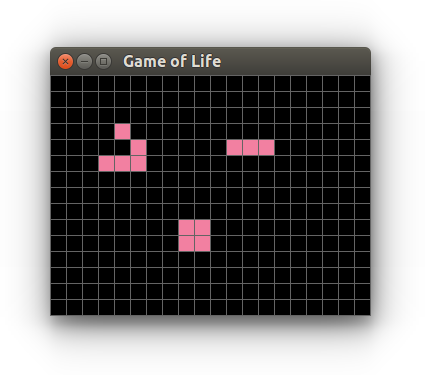
\includegraphics[height=11cm]{../img/glider-blinker-block}
%
\includegraphics[height=4cm]{../img/scala-logo.png}
%
\includegraphics[height=4cm]{../img/java-logo.png}
%
\includegraphics[height=12cm]{cover/gurka.jpg}
}

\author{Björn Regnell}
\date{\raggedbottom%
\vspace{1em}\begin{minipage}{1.0\textwidth}\centering
EDAA45, Lp1-2, HT \CurrentYear\\
Datavetenskap, LTH\\
Lunds universitet\\
~\\
Kompileringsdatum: \today \\
\url{http://cs.lth.se/pgk}
\end{minipage}
}

\usepackage{multicol}

\usepackage{pgffor}  %% http://stackoverflow.com/questions/2561791/iteration-in-latex
%  allows:  \foreach \n in {1,...,4}{ do something with \n }

\usepackage{framed}  %  allows:   \begin{framed}\end{framed}
\FrameSep5pt
\OuterFrameSep0pt

% \newenvironment{Slide}[2][]{%
% \begin{oframed}\setlist{noitemsep}%
% {\vspace{-1.5\topsep}}%tighter frames
% \subsection{#2}%
% }%
% {\end{oframed}} 

\newenvironment{Slide}[2][]{%
%\noindent\rule{\textwidth}{0.4pt}%
\setlist{noitemsep}%
%{\vspace{-1.5\topsep}}%tighter frames
\subsection{#2}%
}%
{~\newline\noindent\rule{\textwidth}{0.4pt}}

% \newcommand{\SlideHeading}[1]{\section*{#1}}

% \usepackage[most]{tcolorbox}
% \newenvironment{Slide}[2][]
%   {\vspace{0.5em}\begin{tcolorbox}[left=1.5em,%width=1.05\textwidth,
%   grow to right by=0.05\textwidth,grow to left by=0.05\textwidth,%
%   %breakable,
%   %frame hidden,
%   colframe=gray!20,
%   enhanced]\setlist{noitemsep}\SlideHeading{#2}}
%   {\end{tcolorbox}\vspace{0.5em}}

\newcommand{\Subsection}[1]{} %ignore slide sections
\newcommand{\SlideOnly}[1]{} %ignore slide font size

\usepackage[framemethod=tikz]{mdframed}


\newif\ifkompendium  % to allow conditional text in slides only showing up in compendium
\kompendiumtrue      % in slides: \kompendiumfalse

\newif\ifPreSolution  % to allow tasks and solutions in same file
\PreSolutiontrue      % in solutions: \PreSolutionfalse

\let\QUESTBEGIN\ifPreSolution  % to mark formatting and numbering of exercises
\let\SOLUTION\else  % to mark solutions in the same file as questions
\let\QUESTEND\fi    % to mark end of exercise

%!TEX encoding = UTF-8 Unicode

\newcommand{\ModWeekONE}{Introduktion}
\newcommand{\ExeWeekONE}{expressions}
\newcommand{\LabWeekONE}{kojo}


\newcommand{\ModWeekTWO}{Program, kontrollstrukturer}
\newcommand{\ExeWeekTWO}{programs}
\newcommand{\LabWeekTWO}{--}


\newcommand{\ModWeekTHREE}{Funktioner, abstraktion}
\newcommand{\ExeWeekTHREE}{functions}
\newcommand{\LabWeekTHREE}{irritext}


\newcommand{\ModWeekFOUR}{Objekt, inkapsling}
\newcommand{\ExeWeekFOUR}{objects}
\newcommand{\LabWeekFOUR}{blockmole}


\newcommand{\ModWeekFIVE}{Klasser, datamodellering}
\newcommand{\ExeWeekFIVE}{classes}
\newcommand{\LabWeekFIVE}{--}


\newcommand{\ModWeekSIX}{Mönster, felhantering}
\newcommand{\ExeWeekSIX}{patterns}
\newcommand{\LabWeekSIX}{blockbattle}


\newcommand{\ModWeekSEVEN}{Sekvenser, enumerationer}
\newcommand{\ExeWeekSEVEN}{sequences}
\newcommand{\LabWeekSEVEN}{shuffle}


\newcommand{\ModWeekEIGHT}{Matriser, typparametrar}
\newcommand{\ExeWeekEIGHT}{matrices}
\newcommand{\LabWeekEIGHT}{life}


\newcommand{\ModWeekNINE}{Mängder, tabeller}
\newcommand{\ExeWeekNINE}{lookup}
\newcommand{\LabWeekNINE}{words}


\newcommand{\ModWeekTEN}{Arv, komposition}
\newcommand{\ExeWeekTEN}{inheritance}
\newcommand{\LabWeekTEN}{snake0}


\newcommand{\ModWeekELEVEN}{Kontextuella abstraktioner, api}
\newcommand{\ExeWeekELEVEN}{context}
\newcommand{\LabWeekELEVEN}{snake1}


\newcommand{\ModWeekTWELVE}{Valfri fördjupning, Projekt}
\newcommand{\ExeWeekTWELVE}{extra}
\newcommand{\LabWeekTWELVE}{Projekt0}


\newcommand{\ModWeekTHIRTEEN}{Repetition}
\newcommand{\ExeWeekTHIRTEEN}{examprep}
\newcommand{\LabWeekTHIRTEEN}{Projekt1}


\newcommand{\ModWeekFOURTEEN}{Muntligt prov}
\newcommand{\ExeWeekFOURTEEN}{Munta}
\newcommand{\LabWeekFOURTEEN}{Munta}


\begin{document}

\pagenumbering{roman}

\frontmatter
\maketitle
%!TEX encoding = UTF-8 Unicode
%!TEX root = ../compendium.tex

\clearpage\null\thispagestyle{empty}
\vfill

{
\setlength{\parindent}{0pt}
\emph{Editor}: Björn Regnell \\

%  LIST OF CONTRIBUTORS to https://github.com/lunduniversity/introprog
%    Please contact bjorn.regnell@cs.lth.se if you think you should be
%    on this list, or make a pull request with an update of file briefly
%    describing your contribtion in the commit text.
%    This work is licenced under CC-BY-SA-4.0.
%!TEX encoding = UTF-8 Unicode
%!TEX root = compendium/compendium.tex
\hyphenation{Borg-lund Da-ne-bjer Grampp Palm-qvist Ravn-borg Ro-sen-qvist Schrei-ter Wih-lan-der}
\emph{Contributors} in alphabetical order:
Anders Buhl,
André Philipsson Eriksson,
Anna Axelsson,
Anna Palmqvist Sjövall,
Anton Andersson,
Benjamin Lindberg,
Björn Regnell,
Casper Schreiter,
Cecilia Lindskog,
Dag Hemberg,
Elliot Bräck,
Elsa Cervetti Ogestad,
Emelie Engström,
Emil Wihlander,
Erik Bjäreholt,
Erik Grampp,
Evelyn Beck,
Fredrik Danebjer,
Gustav Cedersjö,
Henrik Olsson,
Hussein Taher,
Jakob Hök,
Jakob Sinclair,
Johan Ravnborg,
Jonas Danebjer,
Jos Rosenqvist,
Maj Stenmark,
Maria Kulesh,
Måns Magnusson,
Nicholas Boyd Isacsson,
Niklas Sandén,
Oliver Persson,
Oscar Sigurdsson,
Oskar Berg,
Oskar Widmark,
Patrik Persson,
Per Holm,
Philip Sadrian,
Sandra Nilsson,
Sebastian Hegardt,
Simon Persson,
Stefan Jonsson,
Theodor Lundqvist,
Tim Borglund,
Tom Postema,
Valthor Halldorsson,
Viktor Claesson,
Wilhelm Wanecek,
William Karlsson.

\\ \newline

\emph{Home}: \url{https://cs.lth.se/pgk} \newline

\emph{Repo}: \url{https://github.com/lunduniversity/introprog} \\ \newline

This compendium is on-going work. \\ \textbf{Contributions are welcome!} \\
\emph{Contact}: \url{bjorn.regnell@cs.lth.se}
\\ \newline

%\emph{Cover art}: Björn Regnell (inspired by Poul Ströyer's illustration of Lennart Hellsing's lyrics to  the childrens song ''Herr Gurka'' with music by Knut Brodin)\\ \newline

~\\ \newline

You can use this work if you respect this \emph{LICENCE}: CC BY-SA 4.0 \\
\url{http://creativecommons.org/licenses/by-sa/4.0/} \\
Please do \emph{not} distribute your solutions to lab assignments and projects.
\\ \newline
Copyright \copyright~ 2015-2017. \\
Dept. of Computer Science, LTH, Lund University. Lund. Sweden.\\
}

%!TEX encoding = UTF-8 Unicode
%!TEX root = ../compendium.tex

\ChapterUnnum{Framstegsprotokoll} 


\subsubsection*{Genomförda övningar}

\vspace{1em}\noindent 
{Till varje laboration hör en övning med uppgifter som utgör förberedelse inför labben. Du behöver minst behärska grundövningarna för att klara labben inom rimlig tid. Om du känner att du behöver öva mer på grunderna, gör då även extrauppgifterna. Om du vill fördjupa dig, gör fördjupningsuppgifterna som är på mer avancerad nivå. Kryssa för nedan vilka övningar du har gjort, så blir lätt för din handledare att se vilka kunskaper du förvärvat hittills.}

\newcommand{\TickBox}{\raisebox{-.50ex}{\Large$\square$}}
\newcommand{\ExeRow}[1]{\texttt{#1} & \TickBox  &  \TickBox &  \TickBox  \\ \addlinespace }

\begin{table}[h]
\centering
\vspace{2em}
\begin{tabular}{lccc}
\toprule \addlinespace 
{\sffamily\small Övning} & 
{\sffamily\small Grund} &	
{\sffamily\small Extra} &
{\sffamily\small Fördjupning}\\ \addlinespace \midrule \\[-0.7em]
\ExeRow{expressions}
\ExeRow{statements}
\ExeRow{functions}
\ExeRow{data}
\ExeRow{vectors}
\ExeRow{classes}
\ExeRow{traits}
\ExeRow{matching}
\ExeRow{matrices}
\ExeRow{sorting}
\ExeRow{scalajava}
\ExeRow{threads}
\bottomrule
\end{tabular}
\end{table}

\newpage

\subsubsection*{Godkända obligatoriska moment}

\vspace{1em}\noindent 
För att bli godkänd på laborationsuppgifterna och projektuppgiften måste du lösa deluppgifterna och diskutera dina lösningar med en handledare. Denna diskussion är din möjlighet att få feedback på dina lösningar. Ta vara på den!
Se till att handledaren noterar nedan när du blivit godkänd på respektive labb. Spara detta blad tills du fått slutbetyg i kursen. 


\vspace{2.5em}\noindent Namn: \dotfill\\

\vspace{1em}\noindent Namnteckning: \dotfill\\

\newcommand{\LabRow}[1]{\\[-1.1em] \texttt{#1} & \dotfill &  \dotfill  \\ \addlinespace }

\begin{table}[h]
\centering
\vspace{1em}
\begin{tabular}{lcc}
\toprule \addlinespace 
{\sffamily\bfseries\small Lab} & {\sffamily\small Datum gk} &	{\sffamily\small Handledares namnteckning}\\ \addlinespace \midrule \\[-0.5em]
%!TEX encoding = UTF-8 Unicode
%!TEX root = ../compendium2.tex
\LabRow{kojo}
\LabRow{irritext}
\LabRow{blockmole}
\LabRow{blockbattle}
\LabRow{shuffle}
\LabRow{words}
\LabRow{life}
\LabRow{snake}
\LabRow{music}
\LabRow{javatext}
\LabRow{survey}
%\toprule 
\addlinespace \midrule \addlinespace
 \\
{\sffamily\small {\bfseries Projektuppgift} (välj en)	} & \dotfill&\dotfill \\ \addlinespace\addlinespace %\midrule
\texttt{( ) bank}  &  &  \\
\texttt{( ) imageprocessing}  \\
\texttt{( ) tictactoe} \\  
\texttt{( ) }\textit{egendefinerad}  \\
\textit{\small Om egen, ge kort beskrivning:}\\
%\dotfill  \\
\bottomrule
\end{tabular}
\end{table}
%!TEX encoding = UTF-8 Unicode
%!TEX root = ../compendium2.tex


\ChapterUnnum{Förord}

Detta kompendium innehåller övningar och laborationer och övningslösningar för andra läsperioden i LTH:s grundkurs i programmering för civilingenjörsprogrammet Datateknik.


Vi avslutar första läsperioden med en diagnostisk kontrollskrivning där du får återkoppling på vad du lärt dig hittills. Det är viktigt att du använder dina lärdomar om vad du behöver träna mer på och direkt gör upp en plan för hur du kan befästa din förståelse för begreppen i första läsperioden, så att du hänger med under kommande läsperiod.

Det övergripande målet för den andra läsperioden är att du ska kunna skapa egna program som löser mer omfattande problem än tidigare, genom att kombinera flera abstraktionsmekanismer och begrepp från läsperiod 1. Vi inför även nya abstraktionsmekanismer (t.ex. arv), nya språkkonstruktioner (t.ex. mönstermatching), samt jämför och kombinerar Scala och Java. Läsperiod 2 avslutas med ett individuellt projektarbete där du får möjlighet att fördjupa dig enligt dina egna intressen och önskemål.

Kompendiet distribueras som öppen källkod. Det får användas fritt så länge erkännande ges och eventuella ändringar publiceras under samma licens som ursprungsmaterialet. 

I kursens repo \href{http://github.com/lunduniversity/introprog}{github.com/lunduniversity/introprog} finns instruktioner om hur du kan bidra till kursmaterialet.

Välkommen till andra halvlek!

\vspace{1em}\noindent \textit{\hfill Lund, \today, Björn Regnell}


\setcounter{tocdepth}{2} % set headings level in table of contents
\tableofcontents
\mainmatter

\pagenumbering{arabic}


\part{Modulöversikt}

\begin{table}
\noindent\resizebox{1.0\columnwidth}{!}{
\renewcommand{\arraystretch}{2.0}
%!TEX encoding = UTF-8 Unicode
\begin{tabular}{l|l|l|l}
\textit{W} & \textit{Modul} & \textit{Övn} & \textit{Lab} \\ \hline \hline
W01 & Introduktion            & expressions & kojo            \\
W02 & Kodstrukturer           & programs    & --              \\
W03 & Funktioner, Objekt      & functions   & bugs            \\
W04 & Datastrukturer          & data        & pirates         \\
W05 & Sekvensalgoritmer       & sequences   & cards           \\
W06 & Klasser, Likhet         & classes     & turtlegraphics  \\
W07 & Arv, Gränssnitt         & traits      & turtlerace-team \\
KS  & KONTROLLSKRIVN.         & --          & --              \\
W08 & Mönster, Undantag       & matching    & chords-team     \\
W09 & Matriser, Typparametrar & matrices    & maze            \\
W10 & Sökning, Sortering      & sorting     & surveydata-team \\
W11 & Scala och Java          & scalajava   & lthopoly-team   \\
W12 & Trådar                  & threads     & life            \\
W13 & Design                  & Uppsamling  & Projekt         \\
W14 & Tentaträning            & Extenta     & --              \\
T   & TENTAMEN                & --          & --              \\
\end{tabular}

}
\end{table}
\clearpage

\hyphenation{intro-duktion sekvens-algoritmer kod-strukturer data-strukturer}
{\fontsize{11}{12}\selectfont
\renewcommand{\arraystretch}{1.75}
\begin{longtable}{@{}p{.05\textwidth} | >{\hspace{0.1em}\raggedright\bfseries\sffamily}p{.15\textwidth}  >{\raggedleft\arraybackslash\hspace{0.0em}%\fontsize{10.5}{12}\selectfont
}p{0.735\textwidth}}
W01 & Introduktion & sekvens, alternativ, repetition, abstraktion, programmeringsspråk, programmeringsparadigmer, editera-kompilera-exekvera, datorns delar, virtuell maskin, REPL, literal, värde, uttryck, identifierare, variabel, typ, tilldelning, namn, val, var, def, inbyggda typer, Int, Long, Short, Double, Float, Byte, Char, String, println, typen Unit, enhetsvärdet (), stränginterpolatorn s, if, else, true, false, MinValue, MaxValue, aritmetik, slumptal, math.random, logiska uttryck, de Morgans lagar, while-sats, for-sats \\
W02 & Kodstrukturer & iterering, for-uttryck, map, foreach, Range, Array, Vector, algoritm vs implementation, pseudokod, algoritm: SWAP, algoritm: SUM, algoritm: MIN/MAX, algoritm: MININDEX, block, namnsynlighet, namnöverskuggning, lokala variabler, paket, import, filstruktur, jar, dokumentation, programlayout, JDK, main i Java vs Scala, java.lang.System.out.println \\
W03 & Funktioner, objekt & definera funktion, anropa funktion, parameter, returtyp, värdeandrop, namnanrop, default-argument, namngivna argument, applicera funktion på alla element i en samling, procedur, värdeanrop vs namnanrop, uppdelad parameterlista, skapa egen kontrollstruktur, objekt, modul, punktnotation, tillstånd, metod, medlem, funktionsvärde, funktionstyp, äkta funktion, stegad funktion, apply, lazy val, lokala funktioner, anonyma funktioner, lambda, aktiveringspost, anropsstacken, objektheapen, rekursion  cslib.window.SimpleWindow \\
W04 & Datastrukturer & attribut (fält), medlem, metod, tupel, klass, Any, isInstanceOf, toString, case-klass, samling, scala.collection, föränderlighet vs oföränderlighet, List, Vector, Set, Map, typparameter, generisk samling som parameter, översikt samlingsmetoder, översikt strängmetoder, läsa/skriva textfiler, Source.fromFile, java.nio.file \\
W05 & Sekvensalgoritmer & sekvensalgoritm, algoritm: SEQ-COPY, in-place vs copy, algoritm: SEQ-REVERSE, algoritm: SEQ-REGISTER, sekvenser i Java vs Scala, for-sats i Java, java.util.Scanner, scala.collection.mutable.ArrayBuffer, StringBuilder, java.util.Random, slumptalsfrö \\
W06 & Klasser & objektorientering, klass, Point, Square, Complex, new, null, this, inkapsling, accessregler, private, private[this], kompanjonsobjekt, getters och setters, klassparameter, primär konstruktor, objektfabriksmetod, överlagring av metoder, referenslikhet vs strukturlikhet, eq vs == \\
W07 & Arv & arv, polymorfism, trait, extends, asInstanceOf, with, inmixning, supertyp, subtyp, bastyp, override, klasshierarkin i Scala: Any AnyRef Object AnyVal Null Nothing, referenstyper vs värdetyper, klasshierarkin i scala.collection, Shape som bastyp till Point och Rectangle, accessregler vid arv, protected, final, klass vs trait, abstract class, case-object, typer med uppräknade värden \\
KS & \multicolumn{2}{l}{KONTROLLSKRIVN.} \\
W08 & Mönster, undantag & mönstermatchning, match, Option, throw, try, catch, Try, unapply, sealed, flatten, flatMap, partiella funktioner, collect, speciella matchningar: wildcard pattern; variable binding; sequence wildcard; back-ticks, equals, hashcode, exempel: equals för klassen Complex, switch-sats i Java \\
W09 & Matriser, typparametrar & matris, nästlad samling, nästlad for-sats, typparameter, generisk funktion, generisk klass, fri vs bunden typparameter, matriser i Java vs Scala, allokering av nästlade arrayer i Scala och Java \\
W10 & Sökning, sortering & strängjämförelse, compareTo, imlicit ordning, linjärsökning, binärsökning, algoritm: LINEAR-SEARCH, algortim: BINARY-SEARCH, algoritmisk komplexitet, sortering till ny vektor, sortering på plats, insättningssortering, urvalssortering, algoritm: INSERTION-SORT, algoritm: SELECTION-SORT, Ordering[T], Ordered[T], Comparator[T], Comparable[T] \\
W11 & Scala och Java & översikt av syntaxskillnader mellan Scala och Java, klasser i Scala vs Java, referensvariabler vs enkla värden i Java, referenstilldelning vs värdetilldelning i Java, alternativ konstruktor i Scala och Java, for-sats i Java, java for-each i Java, java.util.ArrayList, autoboxing i Java, primitiva typer i Java, wrapperklasser i Java, samlingar i Java vs Scala, scala.collection.JavaConverters, namnkonventioner för konstanter \\
W12 & Webb, trådar & översikt webbprogrammering, kort om html+css+javascript+scala.js, tråd, jämlöpande exekvering, icke-blockerande anrop, callback, java.lang.Thread, java.util.concurrent.atomic.AtomicInteger, scala.concurrent.Future \\
W13 & Design, api & utvecklingsprocessen, krav-design-implementation-test, gränssnitt, trait vs interface, programmeringsgränssnitt (api), designexempel \\
W14 & \multicolumn{2}{l}{Tentaträning} \\
T & \multicolumn{2}{l}{TENTAMEN} \\
\end{longtable}
}

%\renewcommand{\SlideHeading}[1]{\subsection{#1}}  %numbering sections in compendium slides

\part{Moduler}

\setcounter{chapter}{7}

%!TEX encoding = UTF-8 Unicode

%!TEX root = ../compendium1.tex

%!TEX encoding = UTF-8 Unicode
\chapter{Matriser, typparametrar}\label{chapter:W08}
Begrepp som ingår i denna veckas studier:
\begin{itemize}[noitemsep,label={$\square$},leftmargin=*]
\item matris
\item nästlad samling
\item nästlad for-sats
\item typparameter
\item generisk funktion
\item generisk klass
\item fri vs bunden typparameter
\item generiska datastrukturer
\item generiska samlingar i Scala\end{itemize}

\clearpage\section{Teori}
%!TEX encoding = UTF-8 Unicode
%!TEX root = ../lect-w08.tex

%%%

\Subsection{Veckans labb: \texttt{life}}

\begin{Slide}{Veckans labb: \texttt{life}}
\begin{minipage}{0.52\textwidth}
  \setlength{\leftmargini}{0pt}

\begin{itemize}
  \SlideFontSmall
\item Universum är en binär matris av \Emph{celler} där \Emph{levande} celler representeras med \code{true} och \Alert{döda} med \code{false}.
\item Följande regler gäller för \Emph{nästa generation} celler i universum:
\begin{itemize}\SlideFontTiny
  \item \textbf{Fortlevnad}: en levande cell med 2 eller 3 grannar \Emph{lever vidare}
  \item \textbf{Död}: en levande cell med färre än 2 eller fler än 3 grannar \Alert{dör}
  \item \textbf{Födelse}: en död cell med exakt tre grannar föds
\end{itemize}
\item Övning \code{matrices} uppgift 5: skapa en generisk \code{case class Matrix[T]}
\item På labben: använd \code{Matrix[Boolean]}
\end{itemize}

\end{minipage}%
\begin{minipage}{0.5\textwidth}
  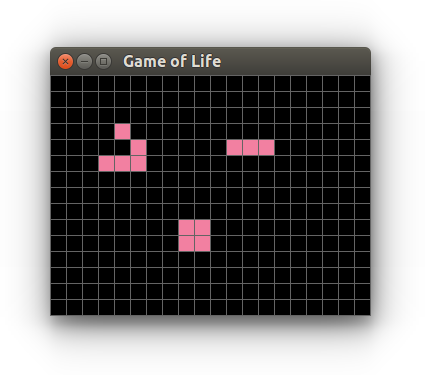
\includegraphics[width=1.0\textwidth]{../img/glider-blinker-block}

  \begin{itemize}\SlideFontTiny
  \item Du ska simulera \emph{Game of Life} i ett \code{introprog.PixelWindow}
  \item Fördjupning:\\{\SlideFontTiny\url{https://en.wikipedia.org/wiki/Conway%27s_Game_of_Life}}
  \end{itemize}
\end{minipage}%

\end{Slide}






\Subsection{Matriser}

\begin{Slide}{Vad är en matris?}\SlideFontSmall
\begin{itemize}

\item En \Emph{matris} inom \Alert{matematiken} innehåller \Emph{rader} och \Emph{kolumner}\footnote{även kallade \emph{kolonner}} med tal.

\item I en \Alert{matematisk} matris har alla rader \Emph{lika många} element och

\item även alla kolumner har \Emph{lika många} element.

\item En matris av dimension $2\times{}5$ har $2 \cdot 5 = 10$ stycken element.

\item Exempel på en matematisk matris av dimension $2\times{}5$:
\[
M_{2,5}=
  \begin{pmatrix}
    5 & 2 & 42 & 4 & 5 \\
    3 & 4 & 18 & 6 & 7
  \end{pmatrix}
\]
\end{itemize}
\end{Slide}

\begin{Slide}{Indexering i en matris}\SlideFontSmall
\begin{itemize}

  \item En matris av dimension $m\times{}n$ har $m \cdot n$ stycken element.

  \item En matris $A_{m,n}$ av dimension $m\times{}n$ ritas inom matematiken ofta så här:

  \[
  A_{m,n} =
   \begin{pmatrix}
    a_{1,1} & a_{1,2} & \cdots & a_{1,n} \\
    a_{2,1} & a_{2,2} & \cdots & a_{2,n} \\
    \vdots  & \vdots  & \ddots & \vdots  \\
    a_{m,1} & a_{m,2} & \cdots & a_{m,n}
   \end{pmatrix}
  \]


\item Matrisindexering inom matematiken sker ofta från $1$, men ofta från $0$ i datorprogram.

\item Vad har talet $42$ för index i matrisen $M_{2,5}$ nedan?
\begin{itemize}\SlideFontTiny
  \item[--] Inom matematiken?
  \item[--] I Scala och Java och många andra språk?

  \[
  M_{2,5}=
    \begin{pmatrix}
      5 & 2 & 42 & 4 & 5 \\
      3 & 4 & 18 & 6 & 7
    \end{pmatrix}
  \]
\end{itemize}
\end{itemize}
\end{Slide}

\begin{Slide}{En matris med array av arrayer}
Inom programmering används ordet \Emph{matris} ofta för att beteckna en \Alert{nästlad struktur} i två dimensioner, till exempel en instans av typen \code{Array[Array[Int]]}
\begin{REPL}
scala> val xss = Array(Array(5,2,42,4,5),Array(3,4,18,6,7))
xss: Array[Array[Int]] = Array(Array(5, 2, 42, 4, 5), Array(3, 4, 18, 6, 7))
\end{REPL}
\pause
Man indexerar i en nästlad sekvens med upprepad \code{apply}:
\begin{REPL}
scala> xss(0)(2)
res0: ???                   // Vad är typ och värde?

scala> xss.apply(0).apply(2)
res1: ???                   // Vad är typ och värde?

scala> xss(0)
res2: ???                   // Vad är typ och värde?
\end{REPL}

\end{Slide}

\begin{Slide}{En matris med array av arrayer}
Inom programmering används ordet \Emph{matris} ofta för att beteckna en \Alert{nästlad struktur} i två dimensioner, till exempel en instans av typen \code{Array[Array[Int]]}
\begin{REPL}
scala> val xss = Array(Array(5,2,42,4,5),Array(3,4,18,6,7))
xss: Array[Array[Int]] = Array(Array(5, 2, 42, 4, 5), Array(3, 4, 18, 6, 7))
\end{REPL}

Man indexerar i en nästlad sekvens med upprepad \code{apply}:
\begin{REPL}
scala> xss(0)(2)
res0: Int = 42

scala> xss.apply(0).apply(2)
res1: Int = 42

scala> xss(0)
res2: Array[Int] = Array(5, 2, 42, 4, 5)
\end{REPL}
\end{Slide}

\begin{Slide}{Uppdatering av en förändringsbar nästlad struktur}
Man kan förändra en array av arrayer ''på plats'' med tilldelning:
\begin{REPL}
scala> val xss = Array(Array(5,2,42,4,5),Array(3,4,18,6,7))

scala> xss(0)(0) = 100

scala> xss
res0: ???

scala> xss(0)(2) = xss(0)(2) - 1

scala> xss
res1: ???

scala> xss(1) = Array.fill(5)(-1)

scala> xss
res2: ???
\end{REPL}
\end{Slide}

\begin{Slide}{Uppdatering av en förändringsbar nästlad struktur}
Man kan förändra en array av arrayer ''på plats'' med tilldelning:
\begin{REPL}
scala> val xss = Array(Array(5,2,42,4,5),Array(3,4,18,6,7))

scala> xss(0)(0) = 100

scala> xss
res0: Array[Array[Int]]=Array(Array(100, 2, 42, 4, 5), Array(3, 4, 18, 6, 7))

scala> xss(0)(2) = xss(0)(2) - 1

scala> xss
res1: Array[Array[Int]]=Array(Array(100, 2, 41, 4, 5), Array(3, 4, 18, 6, 7))

scala> xss(1) = Array.fill(5)(-1)

scala> xss
res2: Array[Array[Int]]=Array(Array(100, 2, 41, 4, 5), Array(-1,-1,-1,-1,-1))
\end{REPL}
\end{Slide}

\begin{Slide}{Några olika sätt att skapa förändringsbara matriser}\SlideFontSmall
Det jobbiga, primitiva sättet:
\begin{REPL}
scala> val xs = new Array[Array[Int]](2)
xs: Array[Array[Int]] = Array(null, null)

scala> for (i <- xs.indices) {xs(i) = new Array[Int](5)}

scala> xs
res0: Array[Array[Int]] = Array(Array(0, 0, 0, 0, 0), Array(0, 0, 0, 0, 0))

scala> println(xs)
[[I@196a99d0
\end{REPL}
Enklare sätt:
\begin{REPL}
scala> val xs = Array.ofDim[Int](2,5)
xs: Array[Array[Int]] = Array(Array(0, 0, 0, 0, 0), Array(0, 0, 0, 0, 0))
\end{REPL}
Enklare och tydligare sätt, där initialvärdet anges explicit:
\begin{REPL}
scala> Array.fill(2,5)(0)
res37: Array[Array[Int]] = Array(Array(0, 0, 0, 0, 0), Array(0, 0, 0, 0, 0))
\end{REPL}

\end{Slide}

\begin{Slide}{Exempel på skapande av oföränderlig nästlad struktur}\SlideFontSmall
Om du kan beräkna initialvärde direkt, använd \code{Vector.fill}:\\
{\SlideFontTiny\code{def fill[A](n1: Int, n2: Int)(elem: => A): Vector[Vector[A]]}}
\begin{REPL}
scala> Vector.fill(2,5)(scala.util.Random.nextInt(6) + 1)
res0:
  typ???
  värde???

\end{REPL}
Om du kan beräkna initialvärde ur index, använd \code{Vector.tabulate}:\\
{\SlideFontTiny\code{def tabulate[A](n1: Int, n2: Int)(f: (Int, Int) => A): Vector[Vector[A]]}}
\begin{REPL}
scala> Vector.tabulate(5,2)((x,y) => x + y + 1)
res1:
  typ???
  värde???

\end{REPL}
\end{Slide}

\begin{Slide}{Exempel på skapande av oföränderlig nästlad struktur}\SlideFontSmall
Om du kan beräkna initialvärde direkt, använd \code{Vector.fill}:\\
{\SlideFontTiny\code{def fill[A](n1: Int, n2: Int)(elem: => A): Vector[Vector[A]]}}
\begin{REPL}
scala> Vector.fill(2,5)(scala.util.Random.nextInt(6) + 1)
res0:
  scala.collection.immutable.Vector[scala.collection.immutable.Vector[Int]] =
  Vector(Vector(1, 2, 6, 2, 1), Vector(1, 4, 3, 3, 2))

\end{REPL}
Om du kan beräkna initialvärde ur index, använd \code{Vector.tabulate}:\\
{\SlideFontTiny\code{def tabulate[A](n1: Int, n2: Int)(f: (Int, Int) => A): Vector[Vector[A]]}}
\begin{REPL}
scala> Vector.tabulate(5,2)((x,y) => x + y + 1)
res1:
  scala.collection.immutable.Vector[scala.collection.immutable.Vector[Int]] =
  Vector(Vector(1,2), Vector(2,3), Vector(3,4), Vector(4,5), Vector(5,	6))

\end{REPL}
\end{Slide}



\begin{Slide}{Uppdatering av en oföränderlig nästlad struktur}\SlideFontSmall
Uppdatering av endimensionell struktur med \code{xs.updated}:\\
{\SlideFontTiny\code{def updated[A](index: Int, elem: A): Vector[A]} }
\begin{REPL}
scala> var xs = Vector.tabulate(5)(x => x + 1)
xs: typ??? = värde???

scala> xs = xs.updated(1, 42)
xs: typ??? = värde???
\end{REPL}

Uppdatering av nästlad struktur i två dimensioner:
\begin{REPL}
scala> var xss = Vector.tabulate(2, 5)((x,y) => x + y + 1)
xss:
  typ??? =
  värde???

scala> xss = xss.updated(0, xss(0).updated(1, 42))
xss:
  typ??? =
  värde???
\end{REPL}

\end{Slide}



\begin{Slide}{Uppdatering av en oföränderlig nästlad struktur}\SlideFontSmall
Uppdatering av endimensionell struktur med \code{xs.updated}:\\
{\SlideFontTiny\code{def updated[A](index: Int, elem: A): Vector[A]} }
\begin{REPL}
scala> var xs = Vector.tabulate(5)(x => x + 1)
xs: scala.collection.immutable.Vector[Int] = Vector(1, 2, 3, 4, 5)

scala> xs = xs.updated(1, 42)
xs: scala.collection.immutable.Vector[Int] = Vector(1, 42, 3, 4, 5)
\end{REPL}

Uppdatering av nästlad struktur i två dimensioner:
\begin{REPL}
scala> var xss = Vector.tabulate(2, 5)((x,y) => x + y + 1)
xss:
  scala.collection.immutable.Vector[scala.collection.immutable.Vector[Int]] =
  Vector(Vector(1, 2, 3, 4, 5), Vector(2, 3, 4, 5, 6))

scala> xss = xss.updated(0, xss(0).updated(1, 42))
xss:
  scala.collection.immutable.Vector[scala.collection.immutable.Vector[Int]] =
  Vector(Vector(1, 42, 3, 4, 5), Vector(2, 3, 4, 5, 6))
\end{REPL}

\end{Slide}


\begin{Slide}{Iterera över nästlad struktur: for-sats}\SlideFontSmall
Iterera med nästlad for-sats:
\begin{REPL}
scala> val xss = Vector.tabulate(2,5)((x,y) => x + y + 1)

scala> for (???) {
         for (???) {
           print(xss(i)(j) + " ")
         }
         println
       }

1 2 3 4 5
2 3 4 5 6
\end{REPL}
\end{Slide}

\begin{Slide}{Iterera över nästlad struktur: for-sats}\SlideFontSmall
Iterera med nästlad for-sats:
\begin{REPL}
scala> val xss = Vector.tabulate(2,5)((x,y) => x + y + 1)

scala> for (i <- xss.indices) {
         for (j <- xss(i).indices) {
           print(xss(i)(j) + " ")
         }
         println
       }

1 2 3 4 5
2 3 4 5 6
\end{REPL}
\end{Slide}


\begin{Slide}{Övningsexempel: Yatzy}\SlideFontSmall
Skapa en funktion \code{roll} som ger utfallet av n st tärningskast:
\begin{REPL}
scala> import scala.util.Random

scala> def roll(n: Int): Vector[Int] = ???
\end{REPL}

Skapa en funktion \code{isYatzy} som ger \code{true} om alla utfall är lika:
\begin{REPL}
scala> def isYatzy(xs: Vector[Int]): Boolean = ???
\end{REPL}
Du kan anta att xs.length > 0\\
Tips: använd metoden xs.forall: \\
\code{def forall[A](p: A => Boolean): Boolean }
\end{Slide}


\begin{Slide}{Övningsexempel: Yatzy}\SlideFontSmall
Skapa en funktion \code{roll} som ger utfallet av n st tärningskast:
\begin{REPL}
scala> import scala.util.Random

scala> def roll(n: Int): Vector[Int] = Vector.fill(n)(Random.nextInt(6) + 1)
\end{REPL}

Skapa en funktion \code{isYatzy} som ger \code{true} om alla utfall är lika:
\begin{REPL}
scala> def isYatzy(xs: Vector[Int]): Boolean = xs.forall(x => x == xs(0))
\end{REPL}
Du kan anta att xs.length > 0\\
Tips: använd metoden xs.forall: \\
\code{def forall[A](p: A => Boolean): Boolean }
\end{Slide}

\begin{Slide}{Iterera över nästlad struktur: for-sats}\SlideFontSmall
Iterera med nästlad for-sats: (vad har xss för typ?)
\begin{REPL}
scala> val xss = Vector.fill(100)(roll(5))

scala> for (???) {
         for (???) {
           print(s"($i)($j) == " + xss(i)(j) + " ")
         }
         println(isYatzy(???))
       }

(0)(0) == 5 (0)(1) == 3 (0)(2) == 4 (0)(3) == 1 (0)(4) == 3 false
(1)(0) == 3 (1)(1) == 3 (1)(2) == 6 (1)(3) == 3 (1)(4) == 1 false
(2)(0) == 3 (2)(1) == 4 (2)(2) == 2 (2)(3) == 2 (2)(4) == 1 false
(3)(0) == 5 (3)(1) == 2 (3)(2) == 6 (3)(3) == 5 (3)(4) == 1 false
(4)(0) == 4 (4)(1) == 6 (4)(2) == 4 (4)(3) == 1 (4)(4) == 4 false
(5)(0) == 3 (5)(1) == 4 (5)(2) == 6 (5)(3) == 5 (5)(4) == 1 false
(6)(0) == 4 (6)(1) == 6 (6)(2) == 2 (6)(3) == 2 (6)(4) == 6 false
(7)(0) == 2 (7)(1) == 5 (7)(2) == 3 (7)(3) == 6 (7)(4) == 2 false
(8)(0) == 4 (8)(1) == 4 (8)(2) == 6 (8)(3) == 1 (8)(4) == 4 false
(9)(0) == 3 (9)(1) == 3 (9)(2) == 3 (9)(3) == 3 (9)(4) == 3 true
(10)(0) == 1 (10)(1) == 2 (10)(2) == 4 (10)(3) == 3 (10)(4) == 3 false
(11)(0) == 6 (11)(1) == 5 (11)(2) == 4 (11)(3) == 1 (11)(4) == 5 false
(12)(0) == 3 (12)(1) == 6 (12)(2) == 6 (12)(3) == 4 (12)(4) == 2 false
\end{REPL}
\end{Slide}

\begin{Slide}{Iterera över nästlad struktur: for-sats}\SlideFontSmall
Iterera med nästlad for-sats: (xss är en \code{Vector[Vector[Int]]})
\begin{REPL}
scala> val xss = Vector.fill(100)(roll(5))

scala> for (i <- xss.indices) {
         for (j <- xss(i).indices) {
           print(s"($i)($j) == " + xss(i)(j) + " ")
         }
         println(isYatzy(xss(i)))
       }

(0)(0) == 5 (0)(1) == 3 (0)(2) == 4 (0)(3) == 1 (0)(4) == 3 false
(1)(0) == 3 (1)(1) == 3 (1)(2) == 6 (1)(3) == 3 (1)(4) == 1 false
(2)(0) == 3 (2)(1) == 4 (2)(2) == 2 (2)(3) == 2 (2)(4) == 1 false
(3)(0) == 5 (3)(1) == 2 (3)(2) == 6 (3)(3) == 5 (3)(4) == 1 false
(4)(0) == 4 (4)(1) == 6 (4)(2) == 4 (4)(3) == 1 (4)(4) == 4 false
(5)(0) == 3 (5)(1) == 4 (5)(2) == 6 (5)(3) == 5 (5)(4) == 1 false
(6)(0) == 4 (6)(1) == 6 (6)(2) == 2 (6)(3) == 2 (6)(4) == 6 false
(7)(0) == 2 (7)(1) == 5 (7)(2) == 3 (7)(3) == 6 (7)(4) == 2 false
(8)(0) == 4 (8)(1) == 4 (8)(2) == 6 (8)(3) == 1 (8)(4) == 4 false
(9)(0) == 3 (9)(1) == 3 (9)(2) == 3 (9)(3) == 3 (9)(4) == 3 true
(10)(0) == 1 (10)(1) == 2 (10)(2) == 4 (10)(3) == 3 (10)(4) == 3 false
(11)(0) == 6 (11)(1) == 5 (11)(2) == 4 (11)(3) == 1 (11)(4) == 5 false
(12)(0) == 3 (12)(1) == 6 (12)(2) == 6 (12)(3) == 4 (12)(4) == 2 false
\end{REPL}
\end{Slide}


\begin{Slide}{Iterera över nästlad struktur med nästlad foreach}\SlideFontSmall
Iterera med nästlad foreach-sats:
\begin{REPL}
scala> val xss = Vector.tabulate(2,5)((x,y) => x + y + 1)

xss.foreach{ xs => ??? ; println }

1 2 3 4 5
2 3 4 5 6
\end{REPL}
\end{Slide}


\begin{Slide}{Iterera över nästlad struktur med nästlad foreach}\SlideFontSmall
Iterera med nästlad foreach-sats:
\begin{REPL}
scala> val xss = Vector.tabulate(2,5)((x,y) => x + y + 1)

xss.foreach{ xs => xs.foreach{ x => print(x + " ") }; println }

1 2 3 4 5
2 3 4 5 6
\end{REPL}
\end{Slide}


\begin{Slide}{Nästlade for-uttryck}\SlideFontSmall
Iterera med \Emph{nästlad for-yield}:\\
%Statisk typ: \code{IndexedSeq[IndexedSeq[[Int]]} \\
%Dynamisk typ: \code{Vector[Vector[[Int]]}

\begin{REPL}
scala> val xss = for (i <- 1 to 2) yield {
                   for (j <- 1 to 5) yield i + j + 1
                 }
xss:
  scala.collection.immutable.IndexedSeq[
    scala.collection.immutable.IndexedSeq[Int]] =
      ???

\end{REPL}
Om man skriver så här får man en endimensionell struktur:
\begin{REPL}
scala> val xs = for (i <- 1 to 2; j <- 1 to 5) yield i + j + 1
xs:
  scala.collection.immutable.IndexedSeq[Int] =
    ???

\end{REPL}
\end{Slide}

\begin{Slide}{Nästlade for-uttryck}\SlideFontSmall
Iterera med \Emph{nästlad for-yield}:\\
\begin{REPL}
scala> val xss = for (i <- 1 to 2) yield {
                   for (j <- 1 to 5) yield i + j + 1
                 }
xss:
  scala.collection.immutable.IndexedSeq[
    scala.collection.immutable.IndexedSeq[Int]] =
      Vector(Vector(3, 4, 5, 6, 7), Vector(4, 5, 6, 7, 8))

\end{REPL}
Om man skriver så här får man en endimensionell struktur:
\begin{REPL}
scala> val xs = for (i <- 1 to 2; j <- 1 to 5) yield i + j + 1
xs:
  scala.collection.immutable.IndexedSeq[Int] =
    Vector(3, 4, 5, 6, 7, 4, 5, 6, 7, 8)

\end{REPL}
\end{Slide}



\begin{Slide}{Nästlade map-uttryck}\SlideFontSmall
Iterera med \Emph{nästlade map-uttryck}:\\
\begin{REPL}
scala> val xss = (1 to 2).map(i => (1 to 5).map(j => i + j + 1))
xss:
  scala.collection.immutable.IndexedSeq[
    scala.collection.immutable.IndexedSeq[Int]] =
      ???
\end{REPL}
\end{Slide}

\begin{Slide}{Nästlade map-uttryck}\SlideFontSmall
Iterera med \Emph{nästlade map-uttryck}:\\
\begin{REPL}
scala> val xss = (1 to 2).map(i => (1 to 5).map(j => i + j + 1))
xss:
  scala.collection.immutable.IndexedSeq[
    scala.collection.immutable.IndexedSeq[Int]] =
      Vector(Vector(3, 4, 5, 6, 7), Vector(4, 5, 6, 7, 8))
\end{REPL}
\end{Slide}




\begin{Slide}{Matris som Array med Array med heltal i Java}\SlideFontTiny
\begin{CodeSmall}[language=Java]
public class ArrayMatrix {

    public static void showMatrix(int[][] m){
        System.out.println("\n--- showMatrix ---");
        for (int row = 0; row < m.length; row++){
            for (int col = 0; col < m[row].length; col++) {
                System.out.print("[" + row + "]");
                System.out.print("[" + col + "] = ");
                System.out.print(m[row][col] + "; ");
            }
            System.out.println();
        }
    }

    public static void main(String[] args) {
        int[][] xss = new int[10][5];
        showMatrix(xss);
    }
}
\end{CodeSmall}
\pause
Övning: skriv en metod \code{fillRnd} som fyller en heltalsmatris med slumptal 1 till n:
\pause
\jcode|public static void fillRnd(int[][] m, int n){ /* ??? */ }| \\
\pause
Tips: använd en nästlad for-sats och: \\
\jcode{(int) (Math.random * n + 1)   // (int) motsvarar Scalas asInstanceOf[Int]}

\end{Slide}

\begin{Slide}{Om veckans övningar}\SlideFontSmall
\begin{itemize}
\item Träna på att iterera i nästlade strukurer

\item Fortsätt jobba med Yatzy-exemplet

\item träna på att skapa \Emph{imperativa} algoritmer: \\
lös \code{isYatzy} med \code{while}-sats (kunde varit del av en tenta...)

\item Extrauppgift där du ska bygga ett enkelt yatzy-spel i terminalen (kunde varit en tentauppgift...)

\end{itemize}
\end{Slide}

% \begin{Slide}{Övning extrauppgift, utgör början på labb \code{survey}}\SlideFontSmall
%
% \begin{ScalaSpec}{Table}
% object Table {
%   /** Creates a new Table from fileName with columns split by sep */
%   def fromFile(fileName: String, separator: Char = ';'): Table = ???
% }
% case class Table(
%   data: Vector[Vector[String]],
%   headings: Vector[String],
%   sep: String){
%   /** A 2-tuple with (number of rows, number of columns) in data */
%   val dim: (Int, Int) = ???
%
%   /** The element in row r an column c of data, counting from 0 */
%   def apply(r: Int, c: Int): String = ???
%
%   /** The row-vector r in data, counting from 0 */
%   def row(r: Int): Vector[String]= ???
%
%   /** The column-vector c in data, counting from 0 */
%   def col(c: Int): Vector[String] = ???
%
%   /** A map from heading to index counting from 0 */
%   lazy val indexOfHeading: Map[String, Int] = ???
%
%   /** The column-vector with heading h in data */
%   def col(h: String): Vector[String] = ???
%
%   /** A vector with the distinct, sorted values of col with heading h */
%   def values(h: String): Vector[String] = ???
%
%   /** Headings and data with columns separated by sep */
%   override lazy val toString: String = ???
% }
% \end{ScalaSpec}
% \end{Slide}


% \begin{Slide}{Övn. fördjupn. uppg.: skapa en generisk matris-klass}\SlideFontSmall
% \vspace{-0.7em}
% \begin{Code}[basicstyle=\SlideFontSize{6}{6.8}\ttfamily\selectfont]
% case class Matrix[T](data: Vector[Vector[T]]){
%
%   def foreachRowCol(f: (Int, Int, T) => Unit): Unit =
%     for (r <- data.indices) {
%       for (c <- data(r).indices) {
%         f(r, c, data(r)(c))
%       }
%     }
%
%   def map[U](f: T => U): Matrix[U] = Matrix(data.map(_.map(f)))
%
%   /** The element at row r and column c */
%   def apply(r: Int, c: Int): T = ???
%
%   /** Gives Some[T](element) at index (r, c) if within index bounds, else None */
%   def get(r: Int, c: Int): Option[T] = ???
%
%   /** The row vector of row r */
%   def row(r: Int): Vector[T] = ???
%
%   /** The column vector of column c */
%   def col(c: Int): Vector[T] = ???
%
%   /** A new Matrix with element at row r and col c updated */
%   def updated(r: Int, c: Int, value: T): Matrix[T] = ???
% }
% object Matrix {
%   def fill[T](rowSize: Int, colSize: Int)(init: T): Matrix[T] =
%     new Matrix(Vector.fill(rowSize)(Vector.fill(colSize)(init)))
% }
% \end{Code}
% \end{Slide}

%!TEX encoding = UTF-8 Unicode
%!TEX root = ../lect-w08.tex

\Subsection{Typparametrar}



\begin{Slide}{Exempel: Icke-generisk case-klass med heltalsmatris}
  En \emph{icke-generisk} datastruktur har inga obundna typparametrar; alla typer är \Emph{konkreta} (alltså specifika). \\~\\ En icke-generisk case-class med en \code{Vector[Vector[Int]]}:
  \begin{Code}
  case class Matrix(data: Vector[Vector[Int]]){
    def apply(x: Int, y: Int): Int = data(x)(y)
  }
  \end{Code}

  \begin{REPL}
  scala> Matrix(Vector(Vector(5, 2, 42, 4, 5),Vector(3, 4, 18, 6, 7)))
  res0: Matrix =
    Matrix(Vector(Vector(5, 2, 42, 4, 5), Vector(3, 4, 18, 6, 7)))
  \end{REPL}

\end{Slide}





\begin{Slide}{Exempel: Generisk case-klass med generell matris}
  En \emph{generisk} datastruktur har en \Emph{typparameter} som är \Alert{abstrakt} (alltså generell) som kan bindas  till ett \Alert{konkret} \Emph{typargument}. \\~\\
  En generisk case-class med en \code{Vector[Vector[T]]}:
  \begin{Code}
  case class Matrix[T](data: Vector[Vector[T]]){
    def apply(x: Int, y: Int): T = data(x)(y)
  }
  \end{Code}

  \begin{REPL}
  scala> Matrix(Vector(Vector(5, 2, 42, 4, 5),Vector(3, 4, 18, 6, 7)))
  res1: Matrix[Int] =
    Matrix(Vector(Vector(5, 2, 42, 4, 5), Vector(3, 4, 18, 6, 7)))
  \end{REPL}

\end{Slide}




\begin{Slide}{Vad är en typparameter?}\SlideFontSmall
  \setlength{\leftmargini}{0pt}

\begin{itemize}
\item En \Emph{typparameter} gör det möjligt att ge ett \Emph{typargument}
\item En \Emph{fri} typparameter kan bindas till vilken typ som helst
\item Bindingen sker vid \Alert{kompileringstid}
\item En typparameter är \Emph{fri} om den \Alert{inte} fått något värde i omslutande deklarationer, annars \Emph{bunden}.
\end{itemize}
Exempel: \Emph{generisk} funktion:
\begin{Code}
def tnirp[A](x: A):Unit = println(x.toString.reverse) // A fri
\end{Code}
\pause
Exempel: \Emph{generisk} klass med generiska metoder:
\begin{Code}
class Cell[A](var value: A){                          // A fri
  def update(x: A): Unit = value = x                  // A bunden
  def create[B](x: B = value): Cell[B] = new Cell(x)  // B fri
}
\end{Code}
\pause
\begin{itemize}
\item \Alert{Skuggning kan förekomma}: Om \code{create} i \code{Cell} hade använt namnet A på sin typparameter hade den \Emph{skuggat} klassens typparameter och tolkats som en  fri typparameter och metoden hade fungerat på samma sätt. (jämför med namnöverskuggning vid lokala variabler i nästlade block)
\end{itemize}

\end{Slide}

\ifkompendium\else
\begin{Slide}{Exempel: Generisk funktion}
Vad händer här?
\begin{REPL}

scala> def skrikBaklänges(x: T): String = x.toString.toUpperCase.reverse
???



scala> def skrikBaklänges[T](x: T): String = x.toString.toUpperCase.reverse

scala> skrikBaklänges("gurka är gott")
res0: ???

\end{REPL}
\end{Slide}


\begin{Slide}{Exempel: Generisk funktion}
Vad händer här?
\begin{REPL}

scala> def skrikBaklänges(x: T): String = x.toString.toUpperCase.reverse
<console>:11: error: not found: type T
       def skrikBaklänges(x: T): String = x.toString.toUpperCase.reverse
                             ^

scala> def skrikBaklänges[T](x: T): String = x.toString.toUpperCase.reverse

scala> skrikBaklänges("gurka är gott")
res0: ???
\end{REPL}
\end{Slide}
\fi

\begin{Slide}{Exempel: Generisk funktion}
Vad händer här?
\begin{REPL}

scala> def skrikBaklänges(x: T): String = x.toString.toUpperCase.reverse
<console>:11: error: not found: type T
       def skrikBaklänges(x: T): String = x.toString.toUpperCase.reverse
                             ^

scala> def skrikBaklänges[T](x: T): String = x.toString.toUpperCase.reverse

scala> skrikBaklänges("gurka är gott")
res0: String = TTOG RÄ AKRUG
\end{REPL}
\end{Slide}

\ifkompendium\else
\begin{Slide}{Exempel: Generisk case-klass}
\vspace{-0.5em}\begin{REPL}
scala> def skrikBaklänges[T](x: T): String = x.toString.toUpperCase.reverse

scala> case class Grönsak(whatever: A)
???


scala> case class Grönsak[A](whatever: A)

scala> Grönsak("gurka")
res1: ???

scala> skrikBaklänges(Grönsak(42))
res2: ???

scala> Grönsak[Int](42)
res3: ???

scala> Grönsak[String](42)
???



                       ^
\end{REPL}
\end{Slide}
\fi

\begin{Slide}{Exempel: Generisk case-klass}
\vspace{-0.5em}\begin{REPL}
scala> def skrikBaklänges[T](x: T): String = x.toString.toUpperCase.reverse

scala> case class Grönsak(whatever: A)
<console>:11: error: not found: type A
       case class Grönsak(whatever: A)
                                    ^
scala> case class Grönsak[A](whatever: A)

scala> Grönsak("gurka")
res1: Grönsak[String] = Grönsak(gurka)

scala> skrikBaklänges(Grönsak(42))
res2: String = )24(KASNÖRG

scala> Grönsak[Int](42)
res3: Grönsak[Int] = Grönsak(42)

scala> Grönsak[String](42)
<console>:14: error: type mismatch;
 found   : Int(42)
 required: String
       Grönsak[String](42)
                       ^
\end{REPL}
\end{Slide}


\ifkompendium\else
\begin{Slide}{Fallgrop: likhet av array}
\begin{REPL}
scala> Vector.fill(5)(42) == Vector.fill(5)(42)
res0: ???

scala> Array.fill(5)(42) == Array.fill(5)(42)
res1: ???
\end{REPL}
\end{Slide}
\fi

\begin{Slide}{Fallgrop: likhet av array}
\begin{REPL}
scala> Vector.fill(5)(42) == Vector.fill(5)(42)
res0: Boolean = true

scala> Array.fill(5)(42) == Array.fill(5)(42)
res1: Boolean = false  // AAAARRGH!!! :(
\end{REPL}
Primitiva arrayer har en equals-metod som ger referenslikhet, \Alert{inte} innehållslikhet.
\end{Slide}

\ifkompendium\else
\begin{Slide}{Kolla likhet av array-matris med nästlad while}
\begin{REPL}
scala> def isEqual(xss: Array[Array[Int]], yss: Array[Array[Int]]) = {
         var i = 0
         var foundUnequal = false
         while (???) {
           var j = 0
           while (???) {
             if (xss(i)(j) != yss(i)(j)) ???
             j += 1
           }
           i += 1
         }
         !foundUnequal
       }

scala> val (xss, yss) = (Array.fill(5,2)(42), Array.fill(5,2)(42))

scala> isEqual(xss, yss)

scala> yss(4)(1) = 0

scala> isEqual(xss, yss)
\end{REPL}
\end{Slide}
\fi


\begin{Slide}{Kolla likhet av array-matris med nästlad while}
\begin{REPL}
scala> def isEqual(xss: Array[Array[Int]], yss: Array[Array[Int]]) = {
         var i = 0
         var foundUnequal = false
         while (i < xss.length && !foundUnequal) {
           var j = 0
           while (j < xss(i).length && !foundUnequal) {
             if (xss(i)(j) != yss(i)(j)) foundUnequal = true
             j += 1
           }
           i += 1
         }
         !foundUnequal
       }

scala> val (xss, yss) = (Array.fill(5,2)(42), Array.fill(5,2)(42))

scala> isEqual(xss, yss)

scala> yss(4)(1) = 0

scala> isEqual(xss, yss)
\end{REPL}
\end{Slide}


\ifkompendium\else
\begin{Slide}{Fördjupning: Fallgrop typradering \Eng{type erasure}}\SlideFontSmall
Informationen om typerna i typparametrar raderas innan kodgenerering av prestandaskäl och \Alert{typparametrar saknas vid runtime}.
\vspace{-0.25em}\begin{REPL}
scala> val xs = Vector(1,2,3)
xs: scala.collection.immutable.Vector[Int] = Vector(1, 2, 3)

scala> val ys = xs.map(_.toDouble)
ys: scala.collection.immutable.Vector[Double] = Vector(1.0, 2.0, 3.0)

scala> def hasDoubles[T](xs: Vector[T]): Boolean = xs match {
         case _: Vector[Int] => false
         case _: Vector[Double] => true
       }

<console>:13: warning: ???


                        ^
<console>:14: warning: ???


                        ^
<console>:14: warning: ???
\end{REPL}
\end{Slide}
\fi

\begin{Slide}{Fördjupning: Fallgrop typradering \Eng{type erasure}}\SlideFontSmall
Informationen om typerna i typparametrar raderas innan kodgenerering av prestandaskäl och \Alert{typparametrar saknas vid runtime}.
\vspace{-0.25em}\begin{REPL}
scala> val xs = Vector(1,2,3)
xs: scala.collection.immutable.Vector[Int] = Vector(1, 2, 3)

scala> val ys = xs.map(_.toDouble)
ys: scala.collection.immutable.Vector[Double] = Vector(1.0, 2.0, 3.0)

scala> def hasDoubles[T](xs: Vector[T]): Boolean = xs match {
         case _: Vector[Int] => false
         case _: Vector[Double] => true
       }

<console>:13: warning: non-variable type argument Int in type pattern scala.collection.immutable.Vector[Int]
is unchecked since it is eliminated by erasure
                case _: Vector[Int] => false
                        ^
<console>:14: warning: non-variable type argument Double in type pattern scala.collection.immutable.Vector[Int]
is unchecked since it is eliminated by erasure
                case _: Vector[Double] => true
                        ^
<console>:14: warning: unreachable code: case _: Vector[Double] => true
\end{REPL}
\end{Slide}

\begin{Slide}{Fördjupning: Dynamisk typtest vid typradering}\SlideFontSmall
Typtest vid körtid med nästlad matchning:
\begin{REPL}
scala> def hasDoubles2[T](xs: Vector[T]): Boolean = xs match {
         case x +: xs => x match {
           case _: Double => true
           case _ => false
         }
         case _ => false
       }

scala> hasDoubles2(Vector(1.0))    // funkar!
\end{REPL}

Typtest vid körtid med match och gard med \code{isInstanceOf}:
\begin{REPL}

scala> def hasDoubles3[T](xs: Vector[T]): Boolean = xs match {
         case x +: xs if x.isInstanceOf[Double] => true
         case _ => false
       }

scala> hasDoubles3(Vector(1.0))    // funkar!


\end{REPL}
\end{Slide}


\ifkompendium\else

\begin{Slide}{Typparametrar på tentan?}
\begin{itemize}
\item Det ingår att kunna använda färdiga generiska strukturer med specifika typer, t.ex. \code{Vector[Int]}

\item Det ingår att kunna skapa strukturer med specifika typparametrar, t.ex. en case-klass som tar en vektor med en specifik typ:\\
\code{case class X(x: Vector[Int])}



\item Det ingår \Alert{inte} på tentan att kunna skapa generiska metoder eller klasser, t.ex.: \\
\code{def f[T](x: Vector[T]): Vector[T] = ???} \\
Mer om generiska strukturer i fördjupningskursen!
\end{itemize}
\end{Slide}

\fi

%!TEX encoding = UTF-8 Unicode
%!TEX root = ../lect-w08.tex

% \Subsection{TODO TABORT Integrerad utvecklingsmiljö (IDE)}

% \begin{Slide}{\TODO TABORT Välja IDE}\SlideFontSmall
% \begin{itemize}
% \item En \Emph{integrerad utvecklingsmiljö} \Eng{Integrated Development Environment, IDE} innehåller \\ editor + kompilator + debugger + en massa annat\\och gör utvecklingen enklare när man lärt sig alla finesser.

% \item Läs om vad en IDE kan göra i appendix.

% \pause

% \item På LTH:s datorer finns tre populära IDE installerade:
% \begin{enumerate}\SlideFontSmall

% \item \Emph{VS Code} med tillägget Metals. \Alert{Rekommenderas!}
% \begin{REPL}[numbers=none]
% > code
% \end{REPL}


% \item \Emph{IntelliJ IDEA} med Scala-plugin. Välj denna om du vill ha en IDE som är mer avancerad och är sugen på att lära dig något nytt.
% \begin{REPL}[numbers=none]
% > idea
% \end{REPL}

% \item \Emph{Eclipse} med plugin \Emph{ScalaIDE} förinstallerad, men rekommenderas ej då den ligger efter i Scala-version.
% \begin{REPL}[numbers=none]
% > scalaide
% \end{REPL}

% \end{enumerate}
% %Läs mer om dessa i appendix.
% %  innan du väljer vilken du vill lära dig.
% % \\Där står även hur du installerar dem på din egen dator.
% % \\IntelliJ anses av många för tillfället ha det bästa Scala-stödet, men är du van vid Eclipse så kanske du vill använda ScalaIDE.
% \end{itemize}
% \end{Slide}

% \begin{Slide}{\TODO SKA HANDLA OM DEBUG i VS Code med Scala-plugin Metals}
% 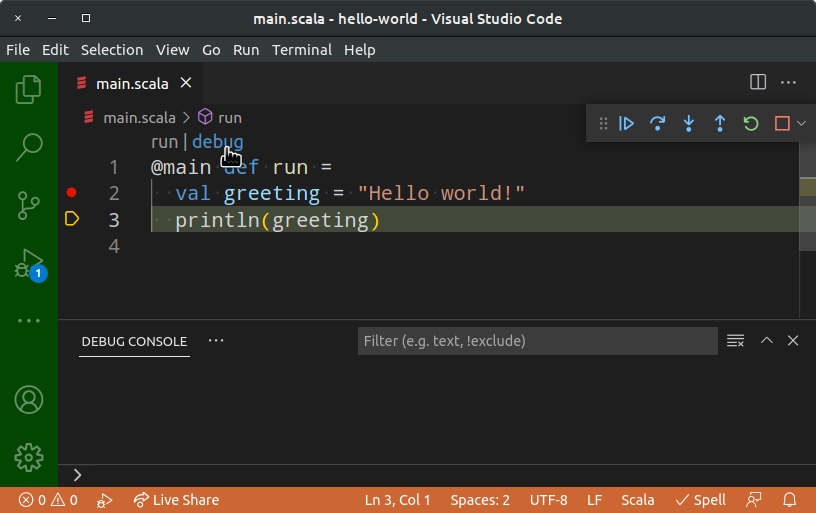
\includegraphics[width=\textwidth]{../img/vscode-debug.png}
% \end{Slide}
  

% \begin{Slide}{IntelliJ IDEA med Scala-plugin}
% 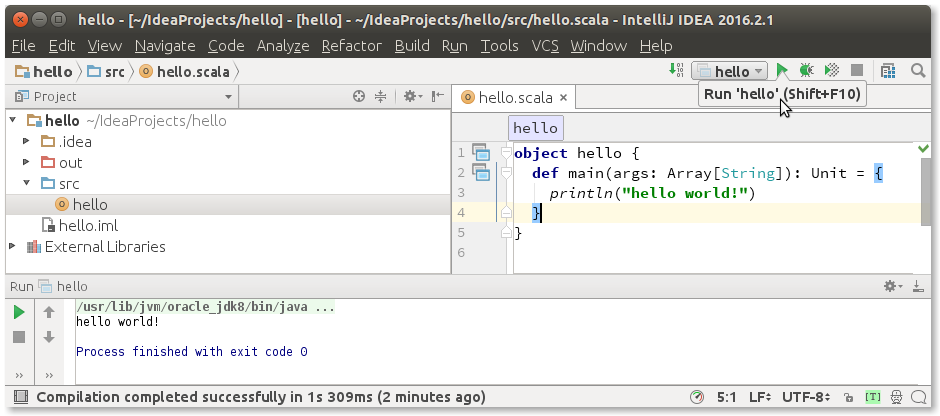
\includegraphics[width=\textwidth]{../img/intellij/idea-hello.png}
% \end{Slide}

% \begin{Slide}{Eclipse med ScalaIDE}
% 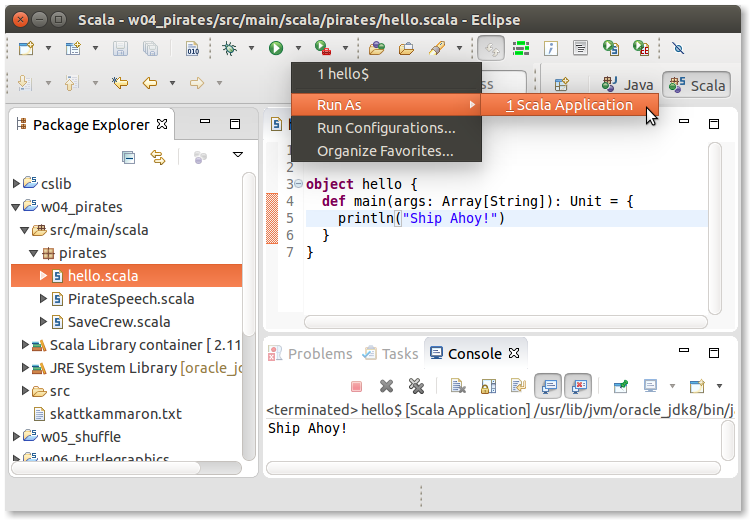
\includegraphics[width=\textwidth]{../img/eclipse/eclipse-pirates-hello.png}
% \end{Slide}



%%!TEX encoding = UTF-8 Unicode
\chapter{Matriser, typparametrar}\label{chapter:W08}
Begrepp som ingår i denna veckas studier:
\begin{itemize}[noitemsep,label={$\square$},leftmargin=*]
\item matris
\item nästlad samling
\item nästlad for-sats
\item typparameter
\item generisk funktion
\item generisk klass
\item fri vs bunden typparameter
\item generiska datastrukturer
\item generiska samlingar i Scala\end{itemize}


%!TEX encoding = UTF-8 Unicode
%!TEX root = ../exercises.tex

\ifPreSolution

\Exercise{\ExeWeekEIGHT}\label{exe:W08}

\begin{Goals}
\item Kunna skapa och använda matriser med nästlade strukturer av \code{Vector}.
\item Kunna iterera över elementen i en matris med nästlade \code{for}-satser och \code{for}-\code{yield}-uttryck, samt nästlad applicering av \code{map} respektive \code{foreach}.
\item Kunna skapa och använda funktioner som tar matriser som parametrar.
\item Kunna skapa en enkel generisk klass och enkla generiska funktioner med hjälp av en typparameter.
\item Kunna beskriva skillnader och likheter mellan Scala och Java vad gäller indexering och iterering i matriser implementerade med nästlade arrayer.
%\item Kunna skapa och använda matriser med hjälp inbyggda arrayer i Java.
%\item Kunna använda nästlade \code{for}-satser i Java för att iterera över elementen i en matris.
\end{Goals}

\begin{Preparations}
\item \StudyTheory{08}
\end{Preparations}

\BasicTasks

\else

\ExerciseSolution{\ExeWeekEIGHT}

\BasicTasks

\fi



\WHAT{Para ihop begrepp med beskrivning.}

\QUESTBEGIN

\Task \what

\vspace{1em}\noindent Koppla varje begrepp med den (förenklade) beskrivning som passar bäst:

\begin{ConceptConnections}
  matris & 1 & & A & konkret typ, binds till typparameter vid kompilering \\ 
  generisk & 2 & & B & indexerbar datastruktur i två dimensioner \\ 
  typargument & 3 & & C & har abstrakt typparameter, typen är generell \\ 
  typhärledning & 4 & & D & kompilatorn beräknar typ ur sammanhanget \\ 
\end{ConceptConnections}

\SOLUTION

\TaskSolved \what

\begin{ConceptConnections}
  matris & 1 & ~~\Large$\leadsto$~~ &  A & indexerbar datastruktur i två dimensioner \\ 
  radvektor & 2 & ~~\Large$\leadsto$~~ &  F & matris av dimension $1\times{}m$ med $m$ horisontella värden \\ 
  kolumnvektor & 3 & ~~\Large$\leadsto$~~ &  G & matris av dimension $m\times{}1$ med $m$ vertikala värden \\ 
  kolonn & 4 & ~~\Large$\leadsto$~~ &  C & annat ord för kolumn \\ 
  generisk & 5 & ~~\Large$\leadsto$~~ &  B & har abstrakt typparameter, typen är generell \\ 
  typargument & 6 & ~~\Large$\leadsto$~~ &  D & konkret typ, binds till typparameter vid kompilering \\ 
  typhärledning & 7 & ~~\Large$\leadsto$~~ &  E & kompilatorn beräknar typ ur sammanhanget \\ 
\end{ConceptConnections}

\QUESTEND




\WHAT{Skapa matriser med hjälp av nästlade samlingar.}

\QUESTBEGIN

\Task  \what~  Man kan i ett datorprogram, med hjälp av samlingar som innehåller samlingar, skapa nästlade strukturer som kan indexeras i två dimensioner och på så sätt representera en  \textbf{matris}.\footnote{\href{https://sv.wikipedia.org/wiki/Matris}{sv.wikipedia.org/wiki/Matris}}

\Subtask Rita minnessituationen efter tilldelningen på rad 1 nedan. Vad har \code{m} för typ och värde? Vad har \code{m} för dimensioner? Hur sker indexeringen i ett datorprogram jämfört med i matematiken?

\begin{REPL}
scala> val m = Vector((1 to 5).toVector, (3 to 7).toVector)
scala> m.apply(0).apply(1)
scala> m(1)
scala> m(1)(4)
\end{REPL}

\Subtask Vad ger uttrycken på raderna 2, 3 och 4 ovan för värden och typ?

\Subtask Man kan i ett datorprogram mycket väl skapa tvådimensionella, nästlade strukturer där raderna \emph{inte} innehåller samma antal element. Det blir då ingen äkta matris i strikt matematisk mening, men man kallar ofta ändå en sådan struktur för en ''matris''. Vilken typ har variablerna \code{m2}, \code{m3}, \code{m4} och \code{m5} nedan?

\begin{REPL}
scala> val m2 = Vector(Vector(1,2,3),Vector(4,5),Vector(42))
scala> val m3 = Vector(Vector(1,2), Vector(1.0, 2.0, 3.0))
scala> val m4 = m3(1) +: Vector("a") +: m3
scala> val m5 = Vector.fill(42){ m2(1).map(e => (e * math.random()).toInt) }
\end{REPL}

\Subtask Vilken av variablerna \code{m2}, \code{m3}, \code{m4} och \code{m5} ovan representerar en äkta matris i matematisk mening? Vilken är dess dimensioner?

\SOLUTION

\TaskSolved \what

\SubtaskSolved   
\includegraphics{../img/w09-solutions/1a} \\
Typ: \code{Vector[Vector[Int]]}\\
Värde: \code{Vector(Vector(1, 2, 3, 4, 5), Vector(3, 4, 5, 6, 7))} \\
Dimensioner: $2 \times 5$\\
Inom matematiken sker indexering enligt konvention med 1 som lägsta index. I scala är lägsta index 0, man använder s.k. 0-indexering. \footnote{Detta är inte fallet i alla programmeringsspråk, vilket du kan läsa mer om på \url{https://en.wikipedia.org/wiki/Array\_data\_type\#Index\_origin}}

\SubtaskSolved
\begin{REPL}
scala> val m = Vector((1 to 5).toVector, (3 to 7).toVector)
m: Vector[Vector[Int]] = Vector(Vector(1, 2, 3, 4, 5), Vector(3, 4, 5, 6, 7))

scala> m.apply(0).apply(1)
res4: Int = 2

scala> m(1)
res5: Vector[Int] = Vector(3, 4, 5, 6, 7)

scala> m(1)(4)
res6: Int = 7
\end{REPL}

\SubtaskSolved  \\
m2: \code{Vector[Vector[Int]]}\\
m3: \code{Vector[Vector[AnyVal]]}\\
m4: \code{Vector[Vector[Any]]}\\
m5: \code{Vector[Vector[Int]]}

\SubtaskSolved  m5, $42 \times 2$

\QUESTEND





\WHAT{Skapa och iterera över matriser.}

\QUESTBEGIN

\Task  \label{matrices:task:yatzy} \what~  Du ska skapa matriser där varje rad representerar 5 kast med en tärning i spelet Yatzy.\footnote{\href{https://sv.wikipedia.org/wiki/Yatzy}{sv.wikipedia.org/wiki/Yatzy}}


\Subtask Definiera i REPL en funktion \code{def throwDie: Int = ???} som returnerar ett slumptal mellan 1 och 6.

\Subtask Skapa nedan heltalsmatris i REPL. Vilken dimension får matrisen?
\begin{REPL}
scala> val ds1 = for (i <- 1 to 1000) yield 
            for (j <- 1 to 5) yield throwDie
          
\end{REPL}

\Subtask Man kan också använda nedan varianter för att skapa en heltalsmatris. Vilken av varianterna \code{ds1} ... \code{ds6} tycker du är lättast att läsa och förstå? Prova respektive variant i REPL och ange vilken typ på \code{ds1} ... \code{ds6} som härleds av kompilatorn.
\begin{REPL}
val ds2 = (1 to 1000).map(i => (1 to 5).map(j => throwDie))
val ds3 = (1 to 1000).map(i => Vector.fill(5)(throwDie))
val ds4 = for (i <- 1 to 1000) yield Vector.fill(5)(throwDie)
val ds5 = Vector.fill(1000)(Vector.fill(5)(throwDie))
val ds6 = Vector.fill(1000, 5)(throwDie)
\end{REPL}


\Subtask Definiera en funktion \\ \code{def roll(n: Int): Vector[Int] = ???}\\ som ger en heltalsvektor med $n$ stycken slumpvisa tärningskast. Kasten ska vara sorterade i växande ordning; använd för detta ändamål samlingsmetoden \code{sorted}.


\Subtask \label{matrices:subtask:isyatzyforall} Definera i REPL en funktion \code{isYatzy(xs: Vector[Int]): Boolean = ???} som testar om alla elementen i en heltalsvektor är samma. Använd samlingsmetoden \code{forall}.


\Subtask Skapa en funktion  \\ \code{def diceMatrix(m: Int, n: Int): Vector[Vector[Int]] = ???} \\ som med hjälp av funktionen \code{roll} skapar en matris med \code{m} st vektorer med vardera \code{n} slumpvisa tärningskast.


\Subtask \label{matrices:subtask:diceMatrixToString} Skapa en funktion som returnerar en utskriftsvänlig sträng \\ \code{def diceMatrixToString(xss: Vector[Vector[Int]]): String = ???} \\med hjälp av \code{map} och \code{mkString}, som fungerar enligt nedan.
\begin{REPL}
scala> val dm2s = diceMatrixToString(diceMatrix(4, 5))
dm2s: String =
2 2 3 3 4
1 2 2 2 5
1 5 5 5 6
1 2 4 5 5
\end{REPL}



\Subtask Implementera funktionen \\ \code{def filterYatzy(xss: Vector[Vector[Int]]): Vector[Vector[Int]]} \\ som filtrerar fram alla yatzy-rader i matrisen \code{xss} enligt nedan. Använd din funktion \code{isYatzy} och samlingsmetoden \code{filter}.
\begin{REPL}
scala> diceMatrixToString(filterYatzy(diceMatrix(10000, 5)))
res18: String =
3 3 3 3 3
2 2 2 2 2
2 2 2 2 2
6 6 6 6 6
3 3 3 3 3
1 1 1 1 1
6 6 6 6 6
\end{REPL}



\Subtask Implementera funktionen \\
\code{def yatzyPips(xss: Vector[Vector[Int]]): Vector[Int] = ???}\\
som ska ge en vektor med de tärningsvärden som gav yatzy, för kasten i matrisen \code{xss} enligt nedan. Använd din funktion \code{filterYatzy}.
\begin{REPL}
scala> val dm = Vector(Vector(1,2,3,4,5),Vector(4,4,4,4,4),Vector(3,3,3,3,3))
scala> yatzyPips(dm)
val res42: Vector[Int] = Vector(4, 3)
\end{REPL}

\SOLUTION

\TaskSolved \what

\SubtaskSolved
\begin{Code}
def throwDie: Int = (math.random() * 6).toInt + 1
\end{Code}
Eller:
\begin{Code}
def throwDie: Int = scala.util.Random.nextInt(6) + 1
\end{Code}

\SubtaskSolved  Matrisdimension i matematisk notation: $1000 \times 5$, vilket motsvarar en matris med 1000 rader och 5 kolumner.

\SubtaskSolved
\begin{Code}
ds1: IndexedSeq[IndexedSeq[Int]]
ds2: IndexedSeq[IndexedSeq[Int]]
ds3: IndexedSeq[Vector[Int]]
ds4: IndexedSeq[Vector[Int]]
ds5: Vector[Vector[Int]]
ds6: Vector[Vector[Int]]
\end{Code}
\code{IndexedSeq} och \code{Vector} ovan finns i paketet \code{scala.collection.immutable}

\SubtaskSolved  \begin{Code}
def roll(n: Int) = Vector.fill(n)(throwDie).sorted
\end{Code}

\SubtaskSolved  \begin{Code}
def isYatzy(xs: Vector[Int]): Boolean = xs.forall(_ == xs(0))
\end{Code}



%2.g)
\SubtaskSolved  \begin{Code}
def diceMatrix(m: Int, n: Int): Vector[Vector[Int]] =
  Vector.fill(m)(roll(n))
\end{Code}

\SubtaskSolved  \begin{Code}
def diceMatrixToString(xss: Vector[Vector[Int]]): String =
  xss.map(_.mkString(" ")).mkString("\n")
\end{Code}


%2.j)
\SubtaskSolved
\begin{Code}
def filterYatzy(xss: Vector[Vector[Int]]): Vector[Vector[Int]] =
  xss.filter(isYatzy)
\end{Code}



%2.m)
\SubtaskSolved  \begin{Code}
def yatzyPips(xss: Vector[Vector[Int]]): Vector[Int] =
  filterYatzy(xss).map(_.head)
\end{Code}

\QUESTEND








\WHAT{En oföränderlig, generisk matris-klass till veckans laboration \hyperref[section:lab:\LabWeekEIGHT]{\texttt{\LabWeekEIGHT}}.}

\QUESTBEGIN

\Task\label{exe:matrices:labprep}  \what~Under veckans laboration ska du simulera en enkel form av ''liv'' som består av celler i ett rutnät. För detta ändamål har vi nytta av en matris-klass som du ska implementera steg för steg i denna övning.
Skapa case-klassen nedan med en editor i filen \code{Matrix.scala}. Testa din lösning med hjälp av valfri \hyperref[appendix:ide]{IDE}, t.ex. \code{scalaide} eller \code{idea}.
\begin{Code}
case class Matrix(data: Vector[Vector[String]]){
  def apply(row: Int, col: Int): String = data(row)(col)
}
object Matrix {
  def fill(dim: (Int, Int))(value: String): Matrix =
    Matrix(Vector.fill(dim._1, dim._2)(value))
}
\end{Code}

\begin{REPLnonum}
scala> val m = Matrix.fill(3,4)("hej")
scala> val e = m(2, 2)
\end{REPLnonum}

\Subtask Vad får \code{m} ovan för typ?

\Subtask Vad får \code{e} ovan för typ?

\Subtask På hur många ställen måste du ändra i \code{Matrix} ovan för att den i stället ska representera en matris av heltal?

\Subtask Du ska nu med hjälp av en \textbf{typparameter} göra \code{Matrix} \textbf{generisk} \Eng{generic}, så att den blir en mer användbar matrisklass som kan innehålla element av vilken typ som helst. Genomför följande ändringar i \code{Matrix.scala}:

\begin{itemize}[noitemsep, nolistsep]
  \item Lägg till en typparameter \code{T} inom klammerparenteser efter namnet \code{Matrix} på alla ställen där det förekommer \emph{utom} efter namnet på kompanjonsobjektet\footnote{Singelobjekt kan inte ha typparametrar, men deras medlemmar kan.}.
  \item Byt ut \code{String} mot \code{T} på alla ställen där \code{String} förekommer.
  \item Lägg till en typparameter \code{T} inom klammerparenteser efter \code{def fill}.
\end{itemize}
Testa din generiska klass i REPL genom att skapa en boolesk matris:
\begin{REPLnonum}
scala> val bm = Matrix.fill(3,4)(false)
scala> val be = bm(0, 0)
\end{REPLnonum}

\Subtask Vad får \code{bm} ovan för typ?

\Subtask Vad får \code{be} ovan för typ?

\Subtask Lägg en kodrad i början av klasskroppen som med hjälp av \code{require} garanterar att alla rader i matrisen är lika långa.

\Subtask Lägg till en medlem \code{val dim: (Int, Int)} i klasskroppen efter \code{require}-satsen som ger ett par (alltså en 2-tupel) med antalet rader resp. kolumner i matrisen.

\Subtask Lägg till en metod \code{def updated(row: Int, col: Int)(value: T): Matrix[T]} som ger en ny matris där element på platsen \code{(row, col)} har uppdaterats till \code{value}.

\Subtask Lägg till en metod \code{def foreachIndex(f: (Int, Int) => Unit): Unit} som för varje index i \code{data} applicerar funktionen \code{f}.

\Subtask Lägg till en metod \code{override def toString} som så att en instans av \code{Matrix} visas enligt följande:
\begin{REPLnonum}
scala> val dm = Matrix.fill(3,4)(42.0)
val dm: Matrix[Double] =
Matrix of dim (3,4):
42.0 42.0 42.0 42.0
42.0 42.0 42.0 42.0
42.0 42.0 42.0 42.0
\end{REPLnonum}


\SOLUTION


\TaskSolved \what

\SubtaskSolved Typen på \code{m} blir \code{Matrix}.

\SubtaskSolved Typen på \code{e} blir \code{String}.

\SubtaskSolved Man behöver ändra på 3 ställen från \code{String} till \code{Int}.

\SubtaskSolved Generisk matris \code{Matrix[T]} för element av godtycklig typ \code{T}:

\begin{CodeSmall}
case class Matrix[T](data: Vector[Vector[T]]):
  def apply(row: Int, col: Int): T = data(row)(col)

object Matrix:
  def fill[T](dim: (Int, Int))(value: T): Matrix[T] =
    Matrix[T](Vector.fill(dim._1, dim._2)(value))
\end{CodeSmall}

\SubtaskSolved Tack vare kompilatorns typinferens så får \code{bm} typen \code{Matrix[Boolean]}.

\SubtaskSolved Typen på \code{be} blir \code{Boolean}.

\noindent \SubtaskSolved \SubtaskSolved \SubtaskSolved \SubtaskSolved \SubtaskSolved är alla implementerade i koden nedan: \vspace{-0.5em}
\begin{CodeSmall}
case class Matrix[T](data: Vector[Vector[T]]):
  require(data.forall(row => row.length == data(0).length))

  val dim: (Int, Int) = (data.length, data(0).length)

  def apply(row: Int, col: Int): T = data(row)(col)

  def updated(row: Int, col: Int)(value: T): Matrix[T] =
    Matrix(data.updated(row, data(row).updated(col, value)))

  def foreachIndex(f: (Int, Int) => Unit): Unit =
    for r <- data.indices; c <- data(r).indices do f(r, c)

  override def toString =
    s"""Matrix of dim $dim:\n${ data.map(_.mkString(" ")).mkString("\n") }"""

object Matrix:
  def fill[T](dim: (Int, Int))(value: T): Matrix[T] =
    Matrix[T](Vector.fill(dim._1, dim._2)(value))

\end{CodeSmall}

\QUESTEND


\clearpage

\ExtraTasks %%%%%%%%%%%%%%%%%%%%%%%%%%%%%%%%%%%%%%%%%%%%%%%%%


\WHAT{Imperativa matrisalgoritmer.}

\QUESTBEGIN

\Task  \what~Imperativa angreppssätt är nödvändiga att kunna när du stöter på samlingar och/eller språk som saknar funktionella metoder och/eller funktionsprogrammeringsmöjligheter. Genom att studera imperativa lösningar till de ofta mer koncisa funktionella lösningarna, får du träning i att skapa algoritmer som använder förändring genom tilldelning vid iterering.

\Subtask Implementera \code{isYatzy} från uppgift \ref{matrices:task:yatzy}\ref{matrices:subtask:isyatzyforall} igen, men nu med ett imperativt angreppssätt som använder en \code{while}-sats i stället för funktionella \code{forall}. Ta hjälp av en variabel \code{i} som håller reda på index och en variabel \code{foundDiff} som håller reda på om ett avvikande värde upptäcks. Funktionen kräver ca 9 rader, så det kan vara lämpligt att öppna en editor att skriva i medan du klurar ut lösningen. Börja med att skriva pseudokod, gärna med penna på papper. Prova genom att klistra in i REPL.

\Subtask En imperativ implementation av \code{diceMatrixToString} från uppgift \ref{matrices:task:yatzy}\ref{matrices:subtask:diceMatrixToString} med hjälp av förändringsbara  \code{StringBuilder}\footnote{\url{https://www.scala-lang.org/api/2.12.9/scala/collection/mutable/StringBuilder.html}} visas nedan. Förklara hur nedan kod fungerar. Vad händer om \code{xss} är tom? Vad händer om \code{xss} bara innehåller tomma vektorer? Nämn en fördel och en nackdel med att använda \code{val sb: StringBuilder} och \code{append}, jämfört med en vanlig, oföränderlig \code{var s: String} och \code{+} för tillägg i slutet.
\begin{Code}
def diceMatrixToString(xss: Vector[Vector[Int]]): String = 
  val sb = new StringBuilder()
  for(m <- xss.indices) do
    for(n <- xss(m).indices) do
      sb.append(xss(m)(n).toString)
      if n < xss(m).size - 1 then sb.append(" ")
      else if m < xss.size - 1 then sb.append("\n")
    end for
  end for
  sb.toString
\end{Code}

\Subtask Gör som träning en imperativ implementation av \code{filterYatzy} med en \code{for}-\code{do}-sats (alltså utan att använda \code{filter}, och utan att använda \code{yield}).


\Subtask Förklara hur nedan funktionella implementation av \code{filterYatzy} med \code{for}-\code{yield}-uttryck fungerar. Tycker du din imperativa lösning är lättare eller svårare att läsa och förstå jämfört nedan funktionella lösning?
\begin{CodeSmall}
def filterYatzy(xss: Vector[Vector[Int]]): Vector[Vector[Int]] = 
  (for i <- xss.indices if isYatzy(xss(i)) yield xss(i)).toVector
\end{CodeSmall}


\SOLUTION

\TaskSolved \what

\SubtaskSolved  \begin{Code}
def isYatzy(xs: Vector[Int]): Boolean = 
  var foundDiff = false
  var i = 0
  while (i < xs.size && !foundDiff) do
    foundDiff = xs(i) != xs(0)
    i += 1
  end while
  !foundDiff
\end{Code}


\SubtaskSolved  Funktionen går igenom varje matrisrad, där den i sin tur går igenom
varje element på raden och lägger till i \code{StringBuilder}-objektet. Om det inte är
det sista elementet på raden läggs även ett blanktecken till, annars läggs ett
nyradstecken till. Undantaget är sista raden, där inget nyradstecken läggs till.
Slutligen konverteras \code{StringBuilder}-objektet till en \code{String} som
returneras.


Är \code{xss} tom blir \code{xss.indices} en tom \code{Range} och den yttre \code{for}-loopen hoppas över och en tom sträng returneras.
Är alla rader tomma hoppas i stället de inre \code{for}-looparna över, med samma resultat.

\emph{Fördel:} \code{StringBuilder} är snabbare vid tillägg på slutet vid stora strängar (men här kommer det inte märkas eftersom strängen är så liten).

\emph{Nackdel:} StringBuilder-koden uppfattas av många som svårare att läsa.

\SubtaskSolved
\begin{Code}
def filterYatzy(xss: Vector[Vector[Int]]): Vector[Vector[Int]] = 
  var result: Vector[Vector[Int]] = Vector()
  for i <- xss.indices if isYatzy(xss(i)) do result = result :+ xss(i)
  result
\end{Code}

\SubtaskSolved  Varje looprunda ger en vektor \code{xss(i)} om filtervillkoret är uppfyllt och resultatet av \code{for}-uttrycket blir en vektor med vektorer som är yatzyslag.

\QUESTEND



\WHAT{Strängtabell med kolumnrubriker.}

\QUESTBEGIN

\Task  \what~  %Denna övning utgör en början på laboration \hyperref[section:lab:survey]{\texttt{survey}} i avsnitt \ref{section:lab:survey} på sidan \pageref{section:lab:survey}.

\Subtask Implementera case-klassen \code{Table} enligt specifikationen nedan. Du kan förutsätta att alla rader har lika många kolumner som antalet element i \code{headings}, samt att alla rubrikerna i \code{headings} är unika. Parametern \code{sep} anger det tecken som används för att separera kolumner. Detta förutsätts också gälla för indatafiler som läses in med \code{fromFile}.

\emph{Tips:}
\begin{itemize}%[nolistsep,noitemsep]
\item Värdet \code{indexOfHeading} kan skapas med hjälp av metoden \code{zipWithIndex} som fungerar på alla sekvenssamlingar, samt metoden \code{toMap} som fungerar på sekvenser av 2-tupler. Undersök först hur metoderna fungerar i REPL och sök upp deras dokumentation.
\item Skapa en indatafil som du kan använda för att testa att \code{Table} fungerar.
\end{itemize}


\begin{CodeSmall}
case class Table(
  data: Vector[Vector[String]],
  headings: Vector[String],
  sep: Char
):
  /** A 2-tuple with (number of rows, number of columns) in data */
  val dim: (Int, Int) = ???

  /** The element in row r and column c of data, counting from 0 */
  def apply(r: Int, c: Int): String = ???

  /** The row-vector r in data, counting from 0 */
  def row(r: Int): Vector[String]= ???

  /** The column-vector c in data, counting from 0 */
  def col(c: Int): Vector[String] = ???

  /** A map from heading to index counting from 0 */
  lazy val indexOfHeading: Map[String, Int] = ???

  /** The column-vector with heading h in data */
  def col(h: String): Vector[String] = ???

  /** A vector with the distinct, sorted values of col with heading h */
  def values(h: String): Vector[String] = ???

  /** Headings and data with columns separated by sep */
  override lazy val toString: String = ???

object Table:
  /** Creates a new Table from fileName with columns split by sep */
  def fromFile(fileName: String, sep: Char = ';'): Table = ???
\end{CodeSmall}

\Subtask Skapa med hjälp av \code{Table} ett program som kan köras från terminalen med \texttt{scala run infile.csv ';'} som ger en utskrift av antalet förekomster av olika värden i respektive kolumn (alltså en variant av registrering).



\SOLUTION

\TaskSolved \what

\SubtaskSolved  \begin{CodeSmall}
case class Table(
  data: Vector[Vector[String]],
  headings: Vector[String],
  sep: Char
):

  val dim: (Int, Int) = (data.size, headings.size)

  def apply(r: Int, c: Int): String = data(r)(c)

  def row(r: Int): Vector[String]= data(r)

  def col(c: Int): Vector[String] = data.map(r => r(c))

  lazy val indexOfHeading: Map[String, Int] = headings.zipWithIndex.toMap

  def col(h: String): Vector[String] = col(indexOfHeading(h))

  def values(h: String): Vector[String] = col(h).distinct.sorted

  override def toString: String =
    val s = sep.toString
    headings.mkString(s) + "\n" +data.map(_.mkString(s)).mkString("\n")

object Table:
  def fromFile(fileName: String, sep: Char = ';'): Table = 
    val lines = scala.io.Source.fromFile(fileName).getLines.toVector
    val matrix= lines.map(_.split(sep).toVector)
    new Table(matrix.tail, matrix.head, sep)
\end{CodeSmall}

\SubtaskSolved  \begin{CodeSmall}
@main 
def run(fileName: String, separator: String): Unit = 
  require(separator.length == 1, "separator ska vara exakt ett tecken")
  val t = Table.fromFile(fileName, separator.head)
  val counts: Vector[Vector[String]] =
    (0 until t.dim._2)
      .map(i => t.values(t.headings(i))
      .map(x => s"$x: ${t.col(i).count(_ == x)}"))
      .toVector
  for (i <- 0 until t.dim._2) do
    println(s"\nColumn: ${i + 1}, ${t.headings(i)}:")
    for (j <- 0 until counts(i).length) do
      println(counts(i)(j))
\end{CodeSmall}

\QUESTEND




\WHAT{Skapa ett yatzy-spel för användning i terminalen.}

\QUESTBEGIN

\Task  \what~%
% \Subtask Skapa en yatzy-matris enligt nedan specifikation. Läs om hur de olika predikaten för att kolla olika giltiga kombinationer i Yatzy ska fungera här: \href{https://en.wikipedia.org/wiki/Yahtzee}{en.wikipedia.org/wiki/Yahtzee}. Bygg ett huvudprogram som testar dina funktioner. Kompilera och testa i terminalen allteftersom du lägger till nya funktioner.
%
% \begin{CodeSmall}
% /** En skiss på en klass som kan användas till ett förenklat yatzy-spel */
% case class YatzyRows(val rows: Vector[Vector[Int]]) {
%   /** A new YatzyRows with a new row of 5 dice rolls appended to rows  */
%   def roll: YatzyRows = ???
%
%   /** A new YatzyRows with some indices of the last row re-rolled  */
%   def reroll(indices: Vector[Int]): YatzyRows = ???
% }
%
% object YatzyRows {
%   def isYatzy(xs: Vector[Int]): Boolean = ???
%   def isThreeOfAKind(xs: Vector[Int]): Boolean = ???
%   def isFourOfAKind(xs: Vector[Int]): Boolean = ???
%   def isFullHouse(xs: Vector[Int]): Boolean = ???
%   def isSmallStraight(xs: Vector[Int]): Boolean = ???
%   def isLargeStraight(xs: Vector[Int]): Boolean = ???
% }
% \end{CodeSmall}
%
%
% \Subtask Använd \code{YatzyRows} för att med hjälp av många tärningskast beräkna sannolikheter för några olika giltiga kombinationer. Använd, om du vill, möjligheten som reglerna ger att slå om tärningar i två ytterliggare kast, där de tärningar som slås om väljs slumpmässigt.
%
%\Subtask
Bygg ett förenklat yatzy-spel i terminalen där användaren kan bestämma vilka tärningar som ska slås om. Börja med något riktigt enkelt och bygg sedan vidare på ditt spel genom att införa fler och fler funktioner.

\SOLUTION


\TaskSolved \what
     %starts with: \emph{Skapa ett yatzy-spel för %%%

 --

% \SubtaskSolved   \begin{CodeSmall}
% /** En skiss på en klass som kan användas till ett förenklat yatzy-spel */
% case class YatzyRows(val rows: Vector[Vector[Int]]) {
%
%   private def throwDie: Int = (math.random() * 6).toInt + 1
%
%   /** A new YatzyRows with a new row of 5 dice rolls appended to rows */
%   def roll: YatzyRows = new YatzyRows(rows :+ Vector.fill(5)(throwDie))
%
%   /** A new YatzyRow with some indices of the last row re-rolled */
%   def reroll(indices: Vector[Int]): YatzyRows =
%     new YatzyRows(rows :+ rows(rows.length - 1).zipWithIndex.map {
%       case (x, i) => if (indices.contains(i)) throwDie else x
%     })
% }
% object YatzyRows {
%
%   def isYatzy(xs: Vector[Int]): Boolean = xs.forall(_ == xs(0))
%
%   def isThreeOfAKind(xs: Vector[Int]): Boolean =
%     xs.exists(x => xs.count(_ == x) >= 3)
%
%   def isFourOfAKind(xs: Vector[Int]): Boolean =
%     xs.exists(x => xs.count(_ == x) >= 4)
%
%   def isFullHouse(xs: Vector[Int]): Boolean =
%     xs.exists(x => xs.count(_ == x) == 3) &&
%     xs.exists(x => xs.count(_ == x) == 2)
%
%   def isSmallStraight(xs: Vector[Int]): Boolean =
%     xs.forall(x => xs.count(_ == x) == 1) && !xs.exists(_ == 6)
%
%   def isLargeStraight(xs: Vector[Int]): Boolean =
%     xs.forall(x => xs.count(_ == x) == 1) && !xs.exists(_ == 1)
% }
%
% \end{CodeSmall}
% Observera att fem stycken 2:or uppfyller kraven för Yatzy, men även för triss och fyrtal.
%
% \SubtaskSolved   Slumpen gör att utfallet inte kommer stämma exakt överens med teorin, men för ett stort antal kast bör resultaten hamna ganska nära. De teoretiska sannolikheterna (utan omkast) finns i \ref{yatzyProb}.
% \begin{table}[h]
% \centering
% \caption{Sannolikhet för olika Yatzy-resultat}
% \label{yatzyProb}
% \begin{tabular}{ll}
% Yatzy&  $0,077\%$  \\
% $\geq3$ av samma& $21\%$\\
% $\geq4$ av samma& $2,0\%$\\
% Kåk& $3,9\%$\\
% Liten stege& $1,5\%$\\
% Stor stege& $1,5\%$
% \end{tabular}
% \end{table}
%
% Kodexempel:
% \begin{CodeSmall}
% import YatzyRows._
%
% object YatzyStats extends App {
%   val n = 1000000.0
%   var yr = YatzyRows(Vector(Vector[Int]()))
%   for (i <- 1 to n.toInt) yr = yr.roll
%   println(s"Yatzy: ${yr.rows.count(isYatzy(_)) / n * 100}%")
%   println(s"Three of a kind: ${yr.rows.count(isThreeOfAKind(_)) / n * 100}%")
%   println(s"Four of a kind: ${yr.rows.count(isFourOfAKind(_)) / n * 100}%")
%   println(s"Full house: ${yr.rows.count(isFullHouse(_)) / n * 100}%")
%   println(s"Small straight: ${yr.rows.count(isSmallStraight(_)) / n * 100}%")
%   println(s"Large straight: ${yr.rows.count(isLargeStraight(_)) / n * 100}%")
% }
% \end{CodeSmall}
%
% \SubtaskSolved  --

\QUESTEND






\clearpage

\AdvancedTasks %%%%%%%%%%%%%%%%%


\WHAT{Generiska funktioner.}

\QUESTBEGIN

\Task  \what~  En generisk funktion har (minst) en typparameter inom klammerparenteser efter namnet, till exempel \code{[T]}. Denna typ förekommer sedan som typ på (någon av) parametrarna i parameterlistan. Kompilatorn härleder en konkret typ vid kompileringstid och ersätter typparametern med denna konkreta typ. På så sätt kan en funktion fungera för många olika typer.

\Subtask Förklara för varje rad nedan vad som händer.

\begin{REPL}
scala> def tnirp[T](x: T): Unit = println(x.toString.reverse)
scala> tnirp(42)
scala> tnirp("hej")
scala> case class Gurka(vikt: Int)
scala> tnirp(Gurka(42))
scala> tnirp[String](42)
scala> tnirp[Double](42)
\end{REPL}

\Subtask Man kan kombinera generiska funktioner med funktioner som tar funktioner som parametrar. Det är så \code{map} och \code{foreach} är implementerade. Förklara för varje rad nedan vad som händer.

\begin{REPL}
scala> def compose[A, B, C](f: A => B, g: B => C)(x: A): C = g(f(x))
scala> def inc(x: Int): Int = x + 1
scala> def half(x: Int): Double = x / 2.0
scala> compose(inc, half)(42)
scala> compose(half, inc)(42)
\end{REPL}

\Subtask Hur lyder felmeddelandet på sista raden ovan? Ändra \code{inc} och/eller \code{half} så att typerna passar.

\SOLUTION

\TaskSolved \what
     %starts with: \emph{Generiska funkioner.} En %%%

%4.a)
\SubtaskSolved   \begin{enumerate}
\item --
\item Strängrepresentationen av \code{42} spegelvänds
\item \code{"hej"} spegelvänds - \code{toString} av en sträng ger en likadan sträng
\item --
\item Gurk-objektets strängrepresentation spegelvänds
\item Funktionens typparameter matchar inte parameterns typ: \code{42} är ingen sträng
\item Implicit typkonvertering till \code{Double} sker för att stämma överens med typparametern, vilket ger en strängrepresentation med decimal
\end{enumerate}

%4.b)
\SubtaskSolved   \begin{enumerate}
\item En funktion definieras så att den tar emot två andra funktioner som argument, sätter ihop dem, och matar in ett tredje argument till den den sammansatta funktionen.
\item En funktion som inkrementerar ett heltal med 1 definieras.
\item En funktion som halverar ett flyttal definieras.
\item \code{42} matas in i \code{inc()} och resultatet (\code{43}) matas vidare till \code{half()}. Inuti \code{half()} sker implicit typkonvertering till \code{Double} då talet divideras med ett flyttal (\code{2.0}) och resultatet blir \code{43.0 / 2.0}, alltså \code{21.5}.
\item Resultatet från \code{half()} är av typ \code{Double}, medan \code{inc()} tar emot ett argument av typ \code{Int}. Då flyttal generellt inte kan konverteras till heltal utan informationsförlust sker ingen implicit konvertering, istället sker ett kompileringsfel.
\end{enumerate}

%4.c)
\SubtaskSolved  \begin{Code}
def inc(x: Double): Double = x + 1.0
\end{Code}
Nu ges kompileringsfel på rad 4 istället, vilket kan lösas med följande ändring:
\begin{Code}
def half(x: Double): Double = x / 2.0
\end{Code}

\QUESTEND




\WHAT{Generiska klasser.}

\QUESTBEGIN

\Task  \what~  Även klasser kan vara generiska. En generisk klass har (minst) en typparameter inom klammerparenteser efter klassens namn.

\Subtask Testa nedan generiska klass \code{Cell[T]} i REPL. Skapa instanser av klassen \code{Cell[T]} där typparametern \code{T} binds till olika konkreta typer och förklara vad som händer.

\begin{REPL}
scala> class Cell[T](var value: T):
         override def toString = "Cell(" + value + ")"
       
scala> new Cell(42)
scala> new Cell("hej")
scala> new Cell(new Cell(math.Pi))
scala> new Cell[String](42)
scala> new Cell[Double](42)
\end{REPL}

\Subtask Lägg till metoden \code{def concat[U](that: Cell[U]):Cell[String]} i klassen \code{Cell} som konkatenerar strängrepresentationerna av de båda cellvärdena.

\begin{REPL}
scala> val a = new Cell("hej")
scala> val b = new Cell(42)
scala> a concat b
\end{REPL}

\Subtask Vilken sorts celler kan du konkatenera om du tar bort typparameternamnet \code{U} i \code{concat} samtidigt som du använder \code{Cell[T]} som typ på värdeparametern \code{that}? Vad ger det för konsekvenser för celler av annan typ än \code{Cell[String]}?

\SOLUTION

\TaskSolved \what

%5.a)
\SubtaskSolved  --

%5.b)
\SubtaskSolved  \begin{Code}
class Cell[T](var value: T):
  override def toString = "Cell(" + value + ")"
  def concat[U](that: Cell[U]): Cell[String] = 
    Cell(s"$value${that.value}")
\end{Code}

%5.c)
\SubtaskSolved   Endast celler med samma typparameter kan nu konkateneras. Eftersom \code{concat()} returnerar ett objekt av typ \code{Cell[String]} kan ett ojämnt antal celler med någon annan typparameter än \code{String} alltså inte längre konkateneras. Är antalet jämnt går det att konkatenera dem parvis och sedan konkatenera de returnerade \code{Cell[String]}-objekten, men det är något omständigt.

\QUESTEND

\WHAT{Implementera fler generiska metoder i \code{Matrix[T]}.}

\QUESTBEGIN

\Task \what~ Bygg vidare på uppgift \ref{exe:matrices:labprep} och implementera nedan specifikation. Skapa egna tester som kontrollerar att alla metoder fungerar som förväntat.

\begin{ScalaSpec}{Matrix[T]}
/** En oföränderlig, generisk Matris-klass. */
case class Matrix[T](data: Vector[Vector[T]]):
  require(???)  // garantera att alla rader har lika många kolumner

  /** Ger ett par med antal rader och kolumner. */
  val dim: (Int, Int) = ???

  /** Ger elementet på plats (row, col). */
  def apply(row: Int, col: Int): T = ???

  /** Ger en ny matris där elementet på plats (row, col) har värdet value. */
  def updated(row: Int, col: Int)(value: T): Matrix[T] =  ???

  /** Applicerar f på alla element. */
  def foreach(f: T => Unit): Unit = ???

  /** Applicerar f på alla index. */
  def foreachIndex(f: (Int, Int) => Unit): Unit = ???

  /** Ger en ny matris med resultaten av elementvis applicering av f. */
  def map[U](f: T => U): Matrix[U] = ???

  /** Ger en ny matris med resultaten av applicering av f på varje index. */
  def mapIndex[U](f: (Int, Int) => U): Matrix[U] = ???

  /** Ger en utskriftsvänlig strängrepresentation av matrisen. */
  override def toString = ???

object Matrix:
  /** Ger en matris med dimension dim där alla element har värdet value. */
  def fill[T](dim: (Int, Int))(value: T): Matrix[T] = ???
\end{ScalaSpec}

\SOLUTION


\TaskSolved \what

\begin{CodeSmall}
case class Matrix[T](data: Vector[Vector[T]]):
  require(data.forall(row => row.size == data(0).size))

  val dim: (Int, Int) = (data.length, data(0).length)

  def apply(row: Int, col: Int): T = data(row)(col)

  def updated(row: Int, col: Int)(value: T): Matrix[T] =
    Matrix(data.updated(row, data(row).updated(col, value)))

  def foreach(f: T => Unit): Unit = data.foreach(_.foreach(f))

  def foreachIndex(f: (Int, Int) => Unit): Unit =
    for r <- data.indices; c <- data(r).indices do f(r, c)

  def map[U](f: T => U): Matrix[U] = Matrix(data.map(_.map(f)))

  def mapIndex[U](f: (Int, Int) => U): Matrix[U] =
    var result = Matrix.fill(dim)(f(0,0))
    for 
      r <- data.indices
      c <- data(r).indices 
    do
      result = result.updated(r, c)(f(r, c))
    end for
    result

  override def toString =
    s"""Matrix of dim $dim:\n${ data.map(_.mkString(" ")).mkString("\n") }"""

object Matrix:
  def fill[T](dim: (Int, Int))(value: T): Matrix[T] =
    Matrix[T](Vector.fill(dim._1, dim._2)(value))
\end{CodeSmall}


\QUESTEND





% \WHAT{Skapa en generisk, oföränderlig matrisklass.}
%
% \QUESTBEGIN
%
% \Task \label{task:generic-matrix} \what~   Med hjälp av en typparameter kan vi skapa en matrisklass som kan innehålla vilka element som helst. Implementera nedan specifikation. Testa din matrisklass i REPL för olika typer av element.
%
% \begin{ScalaSpec}{Matrix[T]}
% case class Matrix[T](data: Vector[Vector[T]]){
%
%   def foreachRowCol(f: (Int, Int, T) => Unit): Unit =
%     for (r <- 0 until data.size) {
%       for (c <- 0 until data(r).size) {
%         f(r, c, data(r)(c))
%       }
%     }
%
%   def map[U](f: T => U): Matrix[U] = Matrix(data.map(_.map(f)))
%
%   /** The element at row r and column c */
%   def apply(r: Int, c: Int): T = ???
%
%   /** Gives Some[T](element) at row r and column c
%    *  if r and c are within index bounds, else None */
%   def get(r: Int, c: Int): Option[T] = ???
%
%   /** The row vector of row r */
%   def row(r: Int): Vector[T] = ???
%
%   /** The column vector of column c */
%   def col(c: Int): Vector[T] = ???
%
%   /** A new Matrix with element at row r and col c updated */
%   def updated(r: Int, c: Int, value: T): Matrix[T] = ???
% }
% object Matrix {
%   def fill[T](rowSize: Int, colSize: Int)(init: T): Matrix[T] =
%     new Matrix(Vector.fill(rowSize)(Vector.fill(colSize)(init)))
% }
% \end{ScalaSpec}
%
% \SOLUTION
%
%
% \TaskSolved \what
%      %%%TODO number  8 %%%starts with: \label{task:generic-matrix} \em%%%
%
% \SubtaskSolved  -- %%%TODO in task 8 %%%
%
%
%
% \QUESTEND
%

% \clearpage
%
% \WHAT{Skapa en Sprite-editor.}
%
% \QUESTBEGIN
%
% \Task  \what~ Använd matrisklassen från uppgift \ref{task:generic-matrix} för att göra en SpriteEditor med JColorChoser enligt nedan skiss.
%
% \begin{Code}
% object ColorChooser {
%   import java.awt.Color
%   import javax.swing.JColorChooser
%
%   var title = "Pick Color"
%   private val chooser = new JColorChooser(Color.BLACK)
%   private val dialog = JColorChooser.
%     createDialog(null, title, true, jcs, null, null)
%
%   def getColor(initColor: Color = Color.BLACK): Color = {
%     chooser.setColor(initColor)
%     dialog.setVisible(true)
%     chooser.getColor
%   }
% }
%
% class Sprite(// en bild med många lager av pixlar i olika färger
%   val id: String,
%   val size: (Int, Int),
%   val pixels: Matrix[Int],   // färg i colors, -1 betyder genomskinlig
%   var scale: Int,            // uppskalning av storlek i pixlar
%   var colors: Vector[Color], // tillgängliga färger
%   var pos: (Int, Int, Int)   // (row, col, layer)
% ){
%   def row = pos._1
%   def col = pos._2
%   def layer = pos._3
% }
%
% class SpriteEditor(
%     rows: Int = 64, cols: Int = 64,
%     scale: Int = 16, nColors: Int = 16) {
%   private val w = new SimpleWindow(???)
%   def edit: Unit = ???
% }
%
% \end{Code}
%
%
%
% \SOLUTION
%
%
% \TaskSolved \what
%      %%%TODO number  9 %%%starts with: \TODO \emph{Klasser för täta oc%%%
%
% \SubtaskSolved  -- %%%TODO in task 9 %%%
%
% \SubtaskSolved  -- %%%TODO in task 9 %%%
%
% \SubtaskSolved  -- %%%TODO in task 9 %%%
%
% \SubtaskSolved  -- %%%TODO in task 9 %%%
%
% \SubtaskSolved  -- %%%TODO in task 9 %%%
%
% \SubtaskSolved  -- %%%TODO in task 9 %%%
%
%
%
% \QUESTEND




% \WHAT{Klasser för täta och glesa matematiska matriser med flyttal.}
%
% \QUESTBEGIN
%
% \Task  \what~   Läs om matrisräkning här: \href{https://sv.wikipedia.org/wiki/Matris}{sv.wikipedia.org/wiki/Matris}
%
% \Subtask Skapa en oföränderlig klass \code{DenseMatrix} för matematiska matriser med dubbelprecisionsflyttal. \code{DenseMatrix} ska internt lagra elementen i en privat \emph{endimensionell} array av flyttal av typen \code{Array[Double]}.
%
% Klassen ska inte vara en case-klass. Det ska gå att skapa matriser med uttryck så som  \code{DenseMatrix.ofDim(3,7)(1.0,42,3.2,1.0,2.2,3)} tack vare ett kompanjonsobjekt med lämplig fabriksmetod som anropar den privata konstruktorn.  Om antalet element är för litet i förhållande till den angivna dimensionen så fyll på med nollor.
%
% \Subtask Överskugga metoderna equals och hashcode och ge \code{DenseMatrix} innehållslikhet i stället för referenslikhet.
%
% \Subtask Implementera egna innehålllikhetsmetoder med namnet \code{===} på \code{DenseMatrix} som är typsäker, d.v.s. bara tillåter innehållsjämförelse mellan täta matriser.
%
% \Subtask Läs om glesa matriser här: \href{https://sv.wikipedia.org/wiki/Gles_matris}{https://sv.wikipedia.org/wiki/Gles\_matris} och implementera \code{SparseMatrix} med ett privat attribut av typen \\ \code{mutable.Map[(Int, Int), Double]} som bara lagrar index som inte är noll.
%
% \Subtask Skapa ett \code{trait Matrix} som både \code{DenseMatrix} och \code{SparseMatrix} ärver, med lämpliga abstrakta och konkreta medlemmar. Implementera addition, subtraktion och multiplikation av täta och glesa matriser.
%
% %\Task \emph{Matriser med \jcode{ArrayList} i Java.} Om man i Java inte vet antalet element i matrisen från början kan man använda en lista av typen \jcode{ArrayList}, där varje element i sin tur innehåller en lista av typen\jcode{ArrayList}. Javas \jcode{ArrayList} är en generisk samling som motsvaras av Scalas \code{ArrayBuffer}. Generiska samlingar i Java kan endast innehålla referenstyper; vill man ha en primitiv typ, t.ex. \jcode{int}, behöver man packa in denna i en s.k. wrapper-klass, t.ex.  klassen \jcode{Integer}. Det finns en wrapper-klass för varje primitiv typ i Java. Matristypen för en heltalstyp i Java skrivs \jcode{ArrayList<ArrayList<Integer>>} där alltså \code{<T>} motsvarar Scalas hakparenteser \code{[T]} för typparametern T.
% %
% %
% %\Subtask \TODO Hitta på deluppgifter med \jcode{ArrayList<ArrayList<Integer>>} som illustrerar ovan. Peka framåt till scalajava-veckan.\SOLUTION
%
% \SOLUTION
%
% \TaskSolved \what
%      %%%TODO number  10 %%%starts with: \emph{Matriser med \jcode{Array%%%
%
% \SubtaskSolved  -- %%%TODO in task 10 %%%
% \QUESTEND

%!TEX encoding = UTF-8 Unicode
%!TEX root = ../compendium2.tex

\Lab{\LabWeekEIGHT}

\begin{Goals}
\item Kunna skapa och använda matriser med hjälp av en generisk datatyp.
\item Kunna iterera över alla element i en matris.
\item Träna på algoritmkonstruktion.
\item Träna på hantering av både oföränderliga och förändringsbara objekt.
\item Använda en integrerad utvecklingsmiljö (IDE).
\end{Goals}

\begin{Preparations}
\item Gör övning {\tt \ExeWeekEIGHT} i kapitel \ref{chapter:W08}, speciellt uppgift \ref{exe:matrices:labprep}.

\item Läs igenom hela laborationen och studera den befintliga koden i \TODO \code{workspace}.

\item Läs appendix \ref{appendix:ide} och välj vilken IDE du ska använda (ScalaIDE/Eclipse eller IntelliJ IDEA). Säkerställ att du får igång en av dessa utvecklingsmijöer genom att köra hello-world-exemplet och sedan ladda ner och importera kursens \TODO workspace enligt instruktionerna i appendix \ref{appendix:ide}.
\end{Preparations}


\begin{figure}[H]
  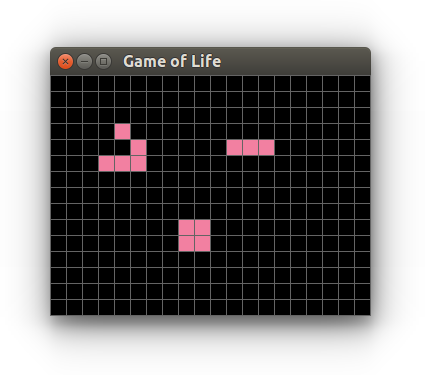
\includegraphics[width=0.8\textwidth]{../img/glider-blinker-block}

  \vspace{-2em}\caption{\label{lab:life:glider-blinker-block}Ett binärt, mörkt datauniversum av dimension $15  \times 20$. Cellkolonin innehåller tre cellgrupper: ett rymdskepp av typen \emph{glider}, en \emph{blinker} och ett \emph{block}.}
\end{figure}


\subsection{Bakgrund}

\emph{Game of Life} simulerar en koloni av encelliga organismer som lever, förökar sig och dör i en matris, enligt några enkla men väl valda regler som konstruerades av matematikern John Horton Conway på 1970-talet. Spelet går ut på att simulera flera generationer utifrån en startkonfiguration, även kallad \emph{cellkoloni}, där varje enskild cells överlevnad beror på dess omgivning. Spelet har inga medvetna spelare och om reglerna följs så kommer slutresultatet enbart bero på startkonfigurationen.

I \emph{Game of Life} består universum av en matris med celler som är antingen levande eller döda. Varje cell har 8 stycken \emph{grannar}, som utgörs av de närmsta omgivande cellerna vertikalt, horisontellt och diagonalt. Varje cells tillstånd i nästa generation bestäms av följande regler:
\begin{enumerate}[nolistsep]
    \item \textbf{Fortlevnad}. Om en levande cell har två eller tre grannar så lever den vidare.
    \item \textbf{Död}. Om en levande cell har mindre än två eller mer än tre grannar så dör den av underpopulation respektive överpopulation.
    \item \textbf{Födelse}. Om cellen är död och har exakt tre grannar så föds den och dess tillstånd ändras till levande, annars fortsätter den vara död.
\end{enumerate}

Flera cellkolonier uppvisar ett ''levande'' beteende där cellmatrisen koloniseras på intressanta vis när en sekvens av generationer visualiseras. Detta är ett exempel på \emph{emergent} beteende där komplexa, självorganiserade strukturer kan uppstå ur enkla förutsättningar.

Läs mer om \emph{Game of Life} på Wikipedia:
\begin{itemize}[noitemsep,topsep=0pt]
    	\item \url{https://en.wikipedia.org/wiki/Conway's_Game_of_Life}
    	\item \url{https://sv.wikipedia.org/wiki/Game_of_Life}
\end{itemize}


\subsection{Obligatoriska krav}

Följande funktionella krav ska uppfyllas av ditt program:
\begin{itemize}[nosep, label={$\square$},]
\item Levande celler ska ha den vackra rosa\footnote{\url{https://www.dsek.se/aktiva/grafiskprofil/farg.php}} RGB-färgen \code{(242, 128, 161)}.
\item Döda celler ska vara svarta som rymden.
\item Detta mörka universum med binära dataceller ska ritas i ett rutnät bestående av smala, stilfulla linjer, så som visas i fig. \ref{lab:life:glider-blinker-block}.
\item Tangenttryckningar och musklick ska fungera enligt följande hjälptext, som ska skrivas ut då programmet startas:
\begin{CodeSmall}
  val help = """
    Welcome to GAME OF LIFE!

    Click on cell to toggle.
    Press ENTER for next generation.
    Press SPACE to toggle play/stop.
    Press R to create random life.
    Press BACKSPACE to clear life.
    Close window to exit.
  """
\end{CodeSmall}
Då \emph{play} aktiveras med blankstegstangenten ska en kontinuerlig simulering av universum fortgå där varje ny generation visualiseras med en lagom fördröjning emellan generationer, tills simuleringen stoppas, t.ex. genom tryck ånyo på blankstegstangenten. Vid varje \emph{Enter}-tryck visas \emph{en} efterkommande generation och ev. pågående simulering stoppas. Vid musklick på en cell ska livstillståndet växlas från levande till död eller vice versa. Ett tryck på R ska ge slumpmässigt liv. Ett tryck på backstegstangenten ska rendera alla universums cellers död.

\end{itemize}

\vspace{1em}\noindent Din kod ska utformas enligt dessa design-krav:
\begin{itemize}[nosep, label={$\square$}]
\item Alla klasser och singelobjekt ska ligga i paketet \code{life}.
\item Det ska finnas en oföränderlig case-klass \code{Life} som representerar ett celluniversum med hjälp av en \code{Matrix[Boolean]} från uppgift \ref{exe:matrices:labprep} i veckans övning.
\item Det ska finnas en klass \code{LifeWindow} som visualiserar en  instans av klassen \code{Life} i ett  \code{introprog.PixelWindow} så som i fig. \ref{lab:life:glider-blinker-block}.
\end{itemize}


\subsection{Valbara krav -- välj minst ett}

Du ska implementera minst ett (gärna flera) av dessa krav:
\begin{itemize}[nosep, label={$\square$}]
\item Cellerna ska färgläggas i olika färger i enlighet med reglerna för nästa generation. Fortlevnad ska fortfarande vara vackert rosa och fortvarig död svart. Följande färger föreslås men välj andra om du tycker det blir finare:
\begin{CodeSmall}
  val UnderPopulated = java.awt.Color.cyan  // en giftig färg
  val OverPopulated  = java.awt.Color.red   // rödklämd av trängsel
  val WillBeBorn     = new java.awt.Color(40, 0, 0)  // snart levande
\end{CodeSmall}
Ge \code{LifeWindow} en klassparameter \code{isMultiColor} som styr om det blir mångfärgade celler eller om det bara finns rosa och svart som i grundkraven.

\item Om man trycker på \code{S} för \emph{Save} ska \code{introprog.Dialog.file("Save Life")} visas och, om användaren inte trycker \Button{Cancel}, det aktuella livet sparas med hjälp av \code{introprog.IO.saveString} i en textfil via metoden \code{toString} i \code{Life}.

\item Om man trycker på \code{O} för \emph{Open} ska \code{introprog.Dialog.file("Open Life")} anropas och ett nytt universum läsas in från textfil enligt lämpligt format. Inläsningen ska ske med hjälp av \code{introprog.IO.loadString} och tolkas till en \code{Life}-instans av en metod i kompanjonsobjektet med detta huvud:
\begin{CodeSmall}
def fromString(s: String, rowDelim: String="\n", alive: Char='0'): Life
\end{CodeSmall}
Testa med filen \texttt{glider-gun.txt} som ska ha följande innehåll på de första 11 raderna och totalt 32 rader där alla rader efter elfte raden innehåller tomt liv:
\begin{REPLnonum}
> head -11 glider-gun.txt
------------------------------------------
-------------------------0----------------
-----------------------0-0----------------
-------------00------00------------00-----
------------0---0----00------------00-----
-00--------0-----0---00-------------------
-00--------0---0-00----0-0----------------
-----------0-----0-------0----------------
------------0---0-------------------------
-------------00---------------------------
------------------------------------------
\end{REPLnonum}
\item Universum ska vara cirkulärt, d.v.s grannen vid kanten finns på andra sidan genom att indexeringen börjar om \Eng{wrapped} enligt modulo-räkning. Inför en klassparameter \code{isWrapped} i \code{Life} och en variabel \code{wrapped: Boolean} i kompanjonsobjektet \code{Life} som styr om fabriksmetoderna skapar ett universum som är cirkulärt eller ej, så att du lätt kan konfigurera detta. \emph{Tips:} Du har stor nytta av att använda \code|java.lang.Math.floorMod| i \code{apply}-metoden i \code{Life}; metoden \code{floorMod} räknar på lämpligt sätt med negativa värden, se dokumentationen för \code{Math}-paketet i JDK8.

\item Läs om varianter till \code{Game of Life} på Wikipedia och implementera alternativa regler som görs valbara genom konfigurering via \code{args}-parametern i \code{main}.

\item Skapa en klass \code{LifeStatistics} som genom väldigt många simuleringar ska ta reda på sannolikheten att en slumpmässig cellkoloni efter $n$ generationer fortfarande utvecklas, respektive är helt dött. Ingen visualisering med \code{PixelWindow} ska ske; endast antalet celler som lever vid generation $n$ och antalet celler som ändrades sedan generation $n - 1$ behöver registreras.

\end{itemize}




\subsection{Tips och förslag}

\begin{enumerate}[leftmargin=*]
\item Här är ett förslag på hur du kan utforma klassen \code{Life}:
\begin{CodeSmall}
package life

case class Life(val cells: Matrix[Boolean]) {

  /** Ger true om cellen på plats (row, col) är vid liv annars false.
    * Ger false om indexeringen är utanför universums gränser.
    */
  def apply(row: Int, col: Int): Boolean = ???

  /** Sätter status på cellen på plats (row, col) till value. */
  def updated(row: Int, col: Int, value: Boolean): Life = ???

  /** Växlar status på cellen på plats (row, col). */
  def toggled(row: Int, col: Int): Life = ???

  /** Räknar antalet levande grannar till cellen i (row, col).*/
  def nbrOfNeighbours(row: Int, col: Int): Int = ???

  /** Skapar en ny Life-instans med nästa generation av universum.
    * Detta sker genom att applicera funktionen \code{rule} på cellerna.
    */
  def evolved(rule: (Int, Int, Life) => Boolean = Life.defaultRule):Life = {
    var nextGeneration = Life.empty(cells.dim)
    cells.foreachIndex { (r,c) =>
      ???
    }
    nextGeneration
  }

  override def toString =
    cells.data.map(_.map(if (_) '0' else '-').mkString).mkString("\n")
}

object Life {
  /** Skapar ett universum med döda celler. */
  def empty(dim: (Int, Int)): Life = ???

  /** Skapar ett unviversum med slumpmässigt liv. */
  def random(dim: (Int, Int)): Life = ???

  /** Implementerar reglerna enligt Conways Game of Life. */
  def defaultRule(row: Int, col: Int, current: Life): Boolean = ???
}
\end{CodeSmall}
Du har nytta av metoden \code{copy} när du implementerar \code{updated} och \code{toggled}. Metoden \code{nbrOfNeighbours} har du nytta av när du ska implementera \code{defaultRule}. När du ska implementera \code{random} har du nytta av metoden \code{foreachIndex} i \code{Matrix[T]}.
Om du som i förslaget ovan låter \code{evolved} ta uppdateringsregeln som en funktionsparameter blir det lättare att konfigurera vilka regler som ska gälla och därmed blir det även lättare att skapa varianter av \emph{Game of Life} genom att införa nya regler i kompanjonsobjektet (se en av de valfria uppgifterna med vidare hänvisning till Wikipedia).

\item Här är ett förslag på hur du kan utforma klassen \code{LifeWindow}:
\begin{CodeSmall}
package life

import introprog.PixelWindow
import introprog.PixelWindow.Event

class LifeWindow(rows: Int, cols: Int){
  import LifeWindow._ // importera konstanter för cellstorlek, färger, etc.

  var life = Life.empty(rows, cols)
  val window: PixelWindow = ???
  var quit = false
  var play = false

  def drawGrid(): Unit = ???

  def drawCell(row: Int, col: Int): Unit = ???

  def update(newLife: Life): Unit = {
    val oldLife = life
    life = newLife
    life.cells.foreachIndex{ ??? }
  }

  def handleKey(key: String): Unit = ???

  def handleClick(pos: (Int, Int)): Unit = ???

  def loopUntilQuit(): Unit = while (!quit) {
    val t0 = System.currentTimeMillis
    if (play) update(life.evolved())
    window.awaitEvent(EventMaxWait)
    while (window.lastEventType != PixelWindow.Event.Undefined) {
      window.lastEventType match {
        case Event.KeyPressed  =>  handleKey(window.lastKey)
        case Event.MousePressed => handleClick(window.lastMousePos)
        case Event.WindowClosed => quit = true
        case _ =>
      }
      window.awaitEvent(EventMaxWait)
    }
    val elapsed = System.currentTimeMillis - t0
    Thread.sleep((NextGenerationDelay - elapsed) max 0)
  }

  def start(): Unit = { drawGrid(); loopUntilQuit() }
}
\end{CodeSmall}

\item \textbf{Dra nytta av den IDE du valt.} Det finns många användbara finesser i en integrerad utvecklingsmiljö. Orientera dig om grunderna genom att läsa appendix \ref{appendix:ide}. Lär dig några viktiga kortkommandon och studera hur du får igång debuggern. Prova att i debuggern sätta brytpunkter, stega dig fram och avläsa variablers värden.
\end{enumerate}

\noindent\TODO Är det för mycket tips? Eller behövs mer tips för att labben ska gå smidigt?


%!TEX encoding = UTF-8 Unicode

%!TEX root = ../compendium1.tex

\chapter{Matriser}
\begin{itemize}[nosep]
\item matriser
\item nästlade for-satser
\item designexempel: Tre-i-rad
\item matriser i Java vs Scala\end{itemize}
\clearpage\section{Teori}
%%!TEX encoding = UTF-8 Unicode
%!TEX root = ../lect-w09.tex


\Subsection{Kontrollskrivning \& Kursmaterial läsperiod 2}

\begin{Slide}{Kontrollskrivning}
Ta med \Alert{legitimation} och \Emph{snabbreferens}, blyertspenna, suddgummi, \Alert{röd} penna till rättningen, förtäring. Ingen mobil. Jackor och väskor vid väggen.
\begin{itemize}
  \item \textbf{Diagnostisk}: vad har du lärt dig hittills?
  \item \textbf{Kamraträttad}: träna på att läsa och bedöma kod
  \item \textbf{Obligatorisk}: sjukdom \Alert{måste} meddelas i förväg
  \item Kan ge \Emph{samarbetsbonus} \Alert{om man har visat samarbetskontrakt}
  %\SlideFontSmall
  \begin{itemize}
    \item[] Max 5p i samarbetsbonus på första ordinarie tentamen, som adderas i slutet av kursen till din tentamenspoäng (max 100) och baseras på \Emph{medelvärdet} av resultaten på kontrollskrivningen i din samarbetsgrupp (se kap ''Anvisningar'' i kompendiet).
  \end{itemize}
\end{itemize}
\end{Slide}

\begin{Slide}{Kontrollskriving -- upplägg}\SlideFontSmall
\begin{itemize}
  \item \textbf{Moment 1}: ca 2 h 15 min: Du löser uppgifterna individuellt
  \item \textbf{Moment 2}: ca 1 h 15 min: Parvis kamratbedömning
  \item \textbf{Moment 3}: ca 30 min: Inspektera din egen skrivning

\item Läs \Alert{noga} igenom instruktionerna på tidigare kontrollskrivning här: 
\url{http://fileadmin.cs.lth.se/pgk/kontroll2017okt24.pdf}

\end{itemize}


\end{Slide}

\begin{Slide}{Plugga i din samarbetsgrupp OCH själv}
\begin{itemize}
\item Träffas och prata \Alert{på rasten} eller enl. ök. om hur ni kan plugga ihop för att maximera lärandet i gruppen!

\pause
\item Träna koda med papper och penna!
\item Tidigare års kontrollskrivningar: \\ \url{http://cs.lth.se/pgk/examination/}

\begin{itemize}
    \item Observera: 2016 ingick \Emph{arv} i lp1 men sedan 2017 kommer detaljerna om \code{extends} och \code{trait} och \code{abstract} i lp2.
\pause
\item Snabbkurs: (så du förstår lite om uppgifterna med arv)
\begin{itemize}\SlideFontSmall
\item Med \code{trait Grönsak} skapas en typ med namnet \code{Grönsak} som kan användas som \Emph{bastyp} i en hierarki av typer.
\item Med \code{extends Grönsak} anges att en typ \Alert{är en} \code{Grönsak}:
\end{itemize}

\end{itemize}

\end{itemize}
\begin{Code}
  trait Grönsak { var vikt: Int }   // alla grönsaker har en vikt
  class Gurka(var vikt: Int) extends Grönsak  // Gurka är en Grönsak
  class Tomat(var vikt: Int) extends Grönsak  // Tomat är en Grönsak
\end{Code}
\end{Slide}


\begin{Slide}{Beställning av tryck av kompendium lp 2}\SlideFontSmall

\begin{itemize}
\item Nu är det dags att beställa tryck av kompendiet del 2 som innehåller
övningar och laborationer inför kommande läsperiod.

\item Beställ här: \url{http://cs.lth.se/pgk/tryck2}

\item Priset är till självkostnad och beror på hur många som beställer.
\item Priset blir max 270kr om färre än 100st beställer
och ca 165kr om minst 100st beställer.

\item Svara *snarast* dock senast 19 Oktober kl 0900.

\item \Alert{Det är himla bra att ha kompendiet på papper, bredvid skärmen speciellt när du jobbar med en IDE med massor av fönster!!}

\end{itemize}
\end{Slide}


\begin{Slide}{Grumligt-lådan}
\begin{itemize}
\item Jag skickar runt \Emph{Grumligt}-lådan.
\item Skriv lappar, \Alert{en lapp per begrepp}, som du tycker är \Emph{''grumligt''} och  önskar förstå bättre.
\item Skicka vidare lådan så fort du är klar.
\item Sista person i salen lämnar tillbaka lådan till mig på rasten.
\item Jag kommer att försöka reda ut några högfrekventa grumligheter på kommande föreläsningar.
\end{itemize}
\end{Slide}

%%!TEX encoding = UTF-8 Unicode
%!TEX root = ../lect-w09.tex


\Subsection{Veckans uppgifter}

\begin{Slide}{Övning: \texttt{lookup}}
\begin{itemize}\SlideFontSmall
  \item Övningen innehåller delar som är \Alert{nödvändiga} för laborationen.
  \item På övningen tränar du på \Emph{mängder} och \Emph{nyckel-värde-tabeller}.
  \item Du ska skapa en klass \code{FreqMapBuilder} som bygger upp en tabell med ordfrekvenser, som behövs på labben.
\end{itemize}
\end{Slide}

\begin{Slide}{Laboration: \texttt{words}}
\begin{itemize}
  \item Denna uppgift handlar om analys av naurligt språk \Eng{Natural Language Processing, NLP}.
  \item Svara på frågorna:
  \begin{itemize}%[noitemsep]
  \item Hur vanligt är ett visst ord i en given text?
  \item Vilket är det vanligaste ordet som följer efter ett visst ord?
  \item Hur kan man generera ordsekvenser som liknar ordföljden i en given text?
  \end{itemize}
\item Använda mängd för unika ord.
\item Använda nyckel-värde-tabell för att för varje ord i en lång text räkna antalet förekomster av detta ord.
\end{itemize}
\end{Slide}


\begin{Slide}{Laboration: \texttt{words}}
Lärandemål:
\begin{itemize}\SlideFontSmall
%!TEX encoding = UTF-8 Unicode
%!TEX root = ../compendium2.tex

%\item Kunna använda en integrerad utvecklingsmiljö (IDE).
%\item Kunna använda färdiga funktioner för att läsa till, och skriva från, textfil.
%\item Kunna använda enkla case-klasser.
%\item Kunna skapa och använda enkla klasser med föränderlig data.
\item Kunna skapa och använda nyckel-värde-tabeller med samlingstypen \code{Map}.
\item Kunna skapa och använda mängder med samlingstypen \code{Set}.
\item Förstå skillnaden mellan en ordnad sekvens och en mängd.
\item Förstå likheter och skillnader mellan en sekvens av par och en nyckel-värde-tabell. 
\item Kunna implementera algoritmer som använder nästlade strukturer. 
%\item Kunna skapa en ny samling från en befintlig samling.
%\item Förstå skillnaden mellan kompileringsfel och exekveringsfel.
%\item Kunna felsöka i små program med hjälp av utskrifter.
%\item Kunna felsöka i små program med hjälp av en debugger i en IDE.

\end{itemize}
Uppgifter:
\begin{itemize}\SlideFontSmall
  \item Dela upp en sträng i ord.
  \item Skapa ordfrekvenstabeller för böcker som ditt program laddar ner från nätet via projektet Gutenberg med fria böcker.
  \item Skapa frekvenstabeller för ordföljder, s.k. \emph{n-gram}.
  \item Skriv ut intressant statistik om ordvalen i olika böcker, t.ex. ur genusperspektiv.
  \item Valfri uppgift: Gör en bot som genererar slumpvisa, artificiella meningar som liknar meningar som människor skriver.
\end{itemize}
\end{Slide}

%!TEX encoding = UTF-8 Unicode
%!TEX root = ../lect-w09.tex


\begin{Slide}{Repetition: Vad är en sekvens?}
\begin{itemize}
\item En sekvens är en \Emph{följd av element} som
  \begin{itemize}
   \item är \Alert{numrerade} (t.ex. från noll), och
   \item är av en viss \Alert{typ} (t.ex. heltal).
  \end{itemize}
  \pause
\item En sekvens kan innehålla \Alert{dubbletter}.
\item En sekvens kan vara \Alert{tom} och ha längden noll.
\item Exempel på en icke-tom sekvens med dubbletter:
\begin{REPLnonum}
scala> val xs = Vector(42, 0, 42, -9, 0, 13, 7)
xs: scala.collection.immutable.Vector[Int] =
  Vector(42, 0, 42, -9, 0, 13, 7)
\end{REPLnonum}
\pause
\item \Emph{Indexering} ger ett element via dess ordningsnummer:
\begin{REPL}
scala> xs(2)
res0: Int = 42

scala> xs.apply(2)
res1: Int = 42
\end{REPL}
\end{itemize}
\end{Slide}




\Subsection{Mängd} %%%%%%%%%%%%%%%%%%%%%%%%%%%%%%%%%%%%%%%%%%%%%%%%%%%%%%


\begin{Slide}{Vad är en mängd?}\SlideFontSmall
\begin{itemize}
\item En \Emph{mängd} är en samling \Alert{unika} element av en viss \Alert{typ}.
\item En mängd kan alltså inte innehålla dubbletter:
\begin{REPLnonum}
scala> Set(1,1,2,2,3,3,4,4,5,5)
res0: scala.collection.immutable.Set[Int] =
  Set(5, 1, 2, 3, 4)
\end{REPLnonum}
\item En mängd är \Alert{inte}  en sekvens: du kan inte utgå från att elementen ligger i någon viss ordning, t.ex. den ordning som de ges vid konstruktion; en mängd har ej längd, men en \Emph{storlek}; metoden \code{size} ger antalet element men metoden \code{length} saknas.
\item Det går \Alert{inte att indexera} i en mängd.
\item Men man \Emph{kan} gå igenom element i \Emph{någon} ordning (exakt vilken är ej def.), med till exempel \code{xs.map(f)} eller \code{for (x <- xs) yield f(x)}
\item En mängd kan vara \Alert{tom} och har då storleken \code{0}.
\pause
\item En mängd \code{Set[T]} med element av typen \code{T} kan ses som ett \Emph{predikat för innehållstest}: alltså en funktion \code{T => Boolean} som är \code{true} om elementet finns annars \code{false}
\end{itemize}
\end{Slide}


\begin{Slide}{Exempel: Oföränderlig mängd}
\setlength{\leftmargini}{1em}
\begin{itemize}
\item \Emph{Skapa}:
\begin{REPLnonum}
scala> var xs = Set("gurka", "tomat", "banan", "pingvin")
\end{REPLnonum}

\item \Emph{Läsa}: avgöra medlemskap
\begin{REPLnonum}
scala> xs("gurka")
res1: Boolean = true
\end{REPLnonum}

\item \Emph{Uppdatera}: lägg till element (händer inget om redan finns)
\begin{REPLnonum}
scala> xs = xs + "jordekorre"
\end{REPLnonum}

\item \Emph{Ta bort}: (om finns, annars händer inget)
\begin{REPLnonum}
scala> xs = xs - "gurka"
\end{REPLnonum}
\end{itemize}
{\SlideFontTiny\code{SLUT} = Skapa, Läsa, Uppdatera, Ta bort \hfill\code{CRUD} = Create, Read, Update, Delete}
\end{Slide}




\begin{Slide}{Exempel: Förändringsbar mängd}\SlideFontSmall
Med en \Alert{förändringsbar} mängd kan man stegvis utöka på plats.
\begin{REPL}
scala> val mängd = scala.collection.mutable.Set.empty[Int]

scala> for (i <- 1 to 1000000) mängd += i

scala> mängd.contains(-1)                     // samma som mängd(-1)
\end{REPL}
En \Emph{mängd} är \Alert{snabb} på att avgöra om ett element \Alert{finns eller inte} i mängden. Ingen linjärsökning krävs eftersom den smarta implementationen av datastrukturen medger snabb uppslagning \Eng{lookup} av ett element.
\pause
\\\vspace{0.5em}Men i en samling krävs linjärsökning vid innehållstest:
\begin{REPL}
scala> val sekvens = (1 to 1000000).toVector

scala> sekvens.contains(-1)   // kräver linjärsökning ända till slutet
\end{REPL}
\pause\SlideFontTiny Övning: Testa själv att mäta tidsskillnaden med hjälp av:
\begin{Code}
def mät(b: => Unit) = 
  { val t1 = System.nanoTime; b; System.nanoTime - t1 }
\end{Code}

\end{Slide}



\begin{Slide}{Mysteriet med de försvunna elementen}
Vad händer här?
\begin{REPLnonum}
scala> val xs1 = Vector(1,2,3,4,5,6)
scala> xs1.map(_ % 2).count(_ == 0)
res0: Int = 3                          // antalet jämna tal
scala> val xs2 = Set(1,2,3,4,5,6)
scala> xs2.map(_ % 2).count(_ == 0)
res1: Int = 1                          // varför?
\end{REPLnonum}
\pause
Mängdegenskaper ger att \code{xs2.map(_ % 2) == Set(0, 1)}\\
Fundera alltid noga på om du \Alert{riskerar att förlora duplikat} som du egentligen hade velat behålla!\\
\pause
Använd \code{toSeq} på mängd om du behöver sekvensegenskaper:
\begin{REPLnonum}
scala> xs2.toSeq.map(_ % 2).count(_ == 0)
res1: Int = 3         // med toSeq blir det som vi ville
\end{REPLnonum}

\end{Slide}




\Subsection{Nyckel-värde-tabell} %%%%%%%%%%%%%%%%%%%%%%%%%%%%%%%%%%%%%%%%


\begin{Slide}{Vad är en nyckel-värde-tabell?}\SlideFontSmall
\begin{itemize}
\item En \Emph{nyckel-värde-tabell} är en samling element som är \Alert{par} med:\\
en \Emph{nyckel} av någon typ \code{K} och ett \Emph{värde} av någon typ \code{V}.
\item En sådan tabell kan skapas ur en sekvens av par \code{(k, v)}\\
där \code{k} är en nyckel och \code{v} är ett värde:
\begin{REPL}
scala> val ålder = Map("Björn" -> 42, "Sandra" -> 35, "Kim" -> 19)
ålder: scala.collection.immutable.Map[String,Int] =
  Map(Björn -> 42, Sandra -> 35, Kim -> 19)
\end{REPL}
\item Tabellens nycklar utgör en mängd som ges av metoden \code{keySet};\\
nycklarna är alltså \Alert{unika}.
\item Elementen utgör \Alert{inte en sekvens} och har ingen speciell ordning;
\\en nyckel-värde-tabell har ej längd, men en \Emph{storlek};\\metoden \code{size} ger antalet element.
\pause
\item En tabell kan ses som en uppslagsfunktion \Eng{dictionary}:\\alltså en funktion \code{K => V} som ger ett värde givet en nyckel.
\end{itemize}
\end{Slide}

%
% \begin{Slide}{Exempel: Nyckel-värde-tabell \TODO}
% \setlength{\leftmargini}{1em}
% \begin{itemize}
% \item \Emph{Skapa}:
% \begin{REPLnonum}
% scala> var xs = ???
% \end{REPLnonum}
%
% \item \Emph{Läsa}: slå upp värde utifrån nyckel
% \begin{REPLnonum}
% scala> xs("gurka")
% \end{REPLnonum}
%
% \item \Emph{Uppdatera}: lägg till mappning (händer inget om redan finns)
% \begin{REPLnonum}
% scala> xs = ???
% \end{REPLnonum}
%
% \item \Emph{Ta bort}: ny tabell utan mappning (om finns, annars händer inget)
% \begin{REPLnonum}
% scala> xs = xs - ???
% \end{REPLnonum}
% \end{itemize}
% {\SlideFontTiny\code{SLUT} = Skapa, Läsa, Uppdatera, Ta bort \hfill\code{CRUD} = Create, Read, Update, Delete}
% \end{Slide}




\begin{Slide}{Den fantastiska nyckel-värde-tabellen \texttt{Map}}\SlideFontSmall
\begin{itemize}
\item En \Emph{nyckel-värde-tabell} \Eng{key-value table} är en slags generaliserad vektor där man kan ''indexera'' med godtycklig typ.

\item Kallas även \href{https://sv.wikipedia.org/wiki/Hashtabell}{\Emph{hashtabell}} \Eng{hash table}, \Emph{lexikon} \Eng{dictionary} eller \Emph{mapp} \Eng{map} (men då blir det lätt sammanblandning med metoden \code{map}).

\item Om man vet nyckeln kan man slå upp värdet \Alert{snabbt}, på liknande sätt som indexering sker i en vektor om man vet heltalsindex.

\item Denna datastruktur är \Alert{mycket användbar} och fungerar som en slags databas i kombination med filtrering, registrering, etc.
\end{itemize}
\begin{REPL}
scala> val födelse = Map("C" -> 1972,  "C++" -> 1983, "C#" -> 2000,
  "Scala" -> 2004, "Java" -> 1995, "Javascript" -> 1995, "Python" -> 1991)

scala> födelse.apply("Scala")
res0: Int = 2004

scala> födelse("Java")
res1: Int = 1995
\end{REPL}
Övning: filtrera ut de språk ovan som kom till efter 1999.
\end{Slide}

\begin{Slide}{Exempel nyckel-värde-tabell}\SlideFontSmall
Några ofta förekommande metoder på tabeller:
\begin{itemize}
\item \code{xs.keySet} ger en mängd av alla nycklar
\item \code{xs.map(f)} mappar funktionen f på alla par av (key, value)
\item \code{xs.mapValues(f)} mappar funktionen f på alla värden
\end{itemize}
\begin{REPL}
scala> val färg = Map("gurka" -> "grön", "tomat"->"röd", "aubergine"->"lila")
färg: scala.collection.immutable.Map[String,String] =
  Map(gurka -> grön, tomat -> röd, aubergine -> lila)

scala> färg("gurka")
res0: String = grön

scala> färg.keySet
res1: scala.collection.immutable.Set[String] = Set(gurka, tomat, aubergine)

scala> val ärGrönSak = färg.map(elem => (elem._1, elem._2 == "grön"))
ärGrönSak: Map[String,Boolean] = Map(gurka -> true, tomat -> false, aubergine -> false)

scala> val baklängesFärg = färg.mapValues(s => s.reverse)
baklängesFärg: Map[String,String] = Map(gurka -> nörg, tomat -> dör, aubergine -> alil)

\end{REPL}

\end{Slide}



\Subsection{\texttt{scala.collection}} %%%%%%%%%%%%%%%%%%%%%%%%%%%%%%%%%%%



% \begin{Slide}{Typparameter möjliggör generiska samlingar}\SlideFontSmall
%
% \begin{itemize}
%   \item Med \Emph{generisk} \Eng{generic} kod menar man att koden kan hantera data av \Alert{godtycklig} typ.
%   \item Funktioner och klasser kan, förutom vanliga parametrar, även ha \Emph{typparametrar} som skrivs i en \Alert{egen} parameterlista med \Alert{hakparenteser} i stället för vanliga parenteser.
%
%   \item En typparameter gör så att funktioner och datastrukturer blir \Emph{generiska}.
%
%   \item Exempel: Funktionerna \code{baklänges} 1--4 nedan är ordnade från specifik typ till mer generell typ.
%
% \begin{Code}
% def baklänges1(xs: Vector[Int]): Vector[Int] = xs.reverse
%
% def baklänges2[T](xs: Vector[T]): Vector[T] = xs.reverse
%
% def baklänges3(xs: Seq[T]): Vector[T] = xs.reverse.toVector
%
% def baklänges4(xs: Seq[T]): Seq[T] = xs.reverse  //reverse avgör samling
% \end{Code}
% \item Mer om typparametrar i w08.
% \end{itemize}
% \end{Slide}



\begin{Slide}{Hierarki av samlingstyper i \texttt{scala.collection} v2.12}

\begin{multicols}{2}
\begin{tikzpicture}[sibling distance=6.1em,->,>=stealth', inner sep=3pt, %scale=0.5,
  every node/.style = {shape=rectangle, draw, align=center,font=\small\ttfamily},
  class/.style = {fill=blue!20},
  trait/.style = {rounded corners, fill=red!20}]
  \node[trait] {Traversable}
    child { node[trait] {Iterable}
      child { node[trait] {Seq}
       }
      child { node[trait] {Set}
      }
      child { node[trait] {Map}
      }
    };
\end{tikzpicture}

\columnbreak

{\SlideFontTiny

\code{Traversable} har metoder som är implementerade med hjälp av: \\
\code{def foreach[U](f: Elem => U): Unit}\\

\vspace{1em}\code{Iterable} har metoder som är implementerade med hjälp av: \\
\code{def iterator: Iterator[A] }

}

\begin{itemize}\SlideFontTiny
\item[] \code{Seq}: ordnade i sekvens
\item[] \code{Set}: unika element
\item[] \code{Map}: par av (nyckel, värde)
\end{itemize}


\end{multicols}

{\SlideFontSmall Samlingen \Emph{\texttt{Vector}} är en \code{Seq} som är en \code{Iterable} som är en \code{Traversable}. \\ \vspace{0.5em}\pause
De konkreta samlingarna är uppdelade i dessa paket:\\
\code{scala.collection.immutable} \hfill som är \Emph{automatiskt} importerade\\
\code{scala.collection.mutable}  \hfill som \Alert{måste importeras} explicit\\\pause
(undantag: primitiva \code{scala.Array} som är automatiskt synlig)
}
\end{Slide}







\begin{Slide}{Använda \texttt{iterator} -- primitiv loop över element}\SlideFontSmall
Med en \code{iterator} kan man \Emph{iterera} med \code{while} över alla element, men endast \Alert{en   gång}; sedan är iteratorn ''förbrukad''. (Men man kan be om en ny.)
\begin{REPL}
scala> val xs = Vector(1,2,3,4)
xs: scala.collection.immutable.Vector[Int] = Vector(1, 2, 3, 4)

scala> val it = xs.iterator
it: scala.collection.immutable.VectorIterator[Int] = non-empty iterator

scala> while (it.hasNext) print(it.next)
1234

scala> it.hasNext
res1: Boolean = false

scala> it.next
java.util.NoSuchElementException: reached iterator end
  at scala.collection.immutable.VectorIterator.next(Vector.scala:674)
\end{REPL}
\Emph{Normalt} behöver man \Alert{inte} använda \code{iterator}: det finns oftast färdiga metoder som gör det man vill, till exempel \code{foreach}, \code{map}, \code{sum}, \code{min} etc.
\end{Slide}






\ifkompendium
\else
\begin{Slide}{Hierarki av samlingar i scala.collection v2.12}\SlideFontTiny
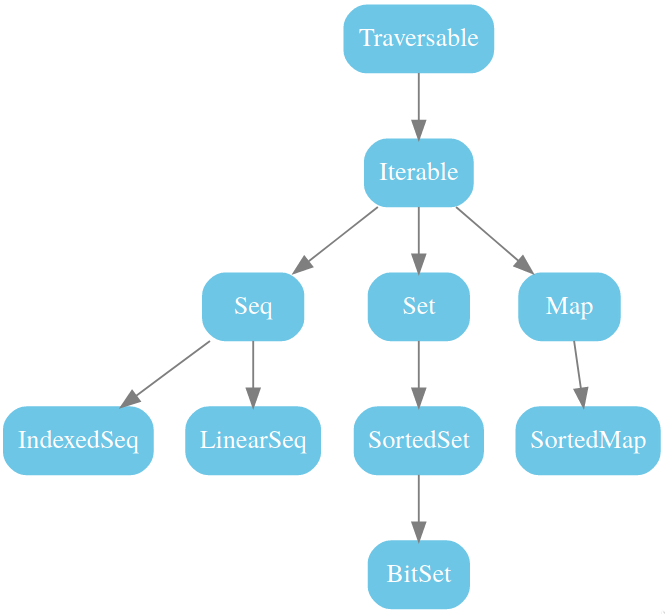
\includegraphics[width=0.95\textwidth]{../img/collection/collection-traits}\\
%\noindent Läs mer om Scalas samlingar här: \\
\url{https://docs.scala-lang.org/overviews/collections/overview.html}
\end{Slide}
\fi





\begin{Slide}{Mer specifika samlingstyper i \texttt{scala.collection} v2.12}
Det finns \Alert{mer specifika} \Emph{subtyper} av \code{Seq}, \code{Set} och \code{Map}:
\\ \vspace{1em}

\begin{tikzpicture}[sibling distance=5.8em,->,>=stealth', inner sep=3pt, %scale=0.5,
  every node/.style = {shape=rectangle, draw, align=center,font=\small\ttfamily},
  class/.style = {fill=blue!20},
  trait/.style = {rounded corners, fill=red!20}]
  \node[trait] {Traversable}
    child { node[trait] {Iterable}
      child { node[trait, xshift=-2.4cm] {Seq}
        child { node[trait] {IndexedSeq} }
        child { node[trait] {LinearSeq} }
       }
      child { node[trait, yshift=-0.0cm] {Set}
        child { node[trait] {SortedSet} }
        child { node[trait] {BitSet} }
      }
      child { node[trait, xshift=1.0cm] {Map}
        child { node[trait] {SortedMap} }
      }
    };
\end{tikzpicture}

\vspace{0.5em}
\Emph{\texttt{Vector}} är en \Alert{\texttt{IndexedSeq}} medan
\Emph{\texttt{List}} är en \Alert{\texttt{LinearSeq}}.
\end{Slide}

\begin{Slide}{Några oföränderliga och förändringsbara sekvenssamlingar}\SlideFontSmall
\begin{tabular}{r l l}
\texttt{scala.collection.\Emph{immutable}.Seq.} & & \\
 & \code|IndexedSeq.| & \\
 & & \Emph{\texttt{Vector}} \\
 & & \Emph{\texttt{Range}} \\
 & \code|LinearSeq.| & \\
 & & \Emph{\texttt{List}} \\
   & & \Emph{\texttt{Queue}} \\

\texttt{scala.collection.\Alert{mutable}.Seq.} & & \\
 & \code|IndexedSeq.| & \\
 & & \Alert{\texttt{ArrayBuffer}} \\
 & & \Alert{\texttt{StringBuilder}} \\
 & \code|LinearSeq.| & \\
 & & \Alert{\texttt{ListBuffer}} \\
   & & \Alert{\texttt{Queue}} \\
\end{tabular}

Fördjupning: Studera samlingars prestandaegenskaper här:\\ \href{https://docs.scala-lang.org/overviews/collections/performance-characteristics.html}{docs.scala-lang.org/overviews/collections/performance-characteristics.html}
\end{Slide}



\begin{Slide}{Några användbara metoder på samlingar}\SlideFontTiny
\begin{tabular}{r r l}\hline
\texttt{\Emph{Traversable}}
  & \code|xs.size| & antal elementet \\
  & \code|xs.head| & första elementet \\
  & \code|xs.last| & sista elementet \\
  & \code|xs.take(n)| & ny samling med de första n elementet \\
  & \code|xs.drop(n)| & ny samling utan de första n elementet \\
  & \code|xs.foreach(f)| & gör \code|f| på alla element, returtyp \code|Unit|\\
  & \code|xs.map(f)| & gör \code|f| på alla element, ger ny samling \\
  & \code|xs.filter(p)| & ny samling med bara de element där p är sant\\
  & \code|xs.groupBy(f)| & ger en \code|Map| som grupperar värdena enligt f\\
  & \code|xs.mkString(",")| & en kommaseparerad sträng med alla element\\ \hline

\texttt{\Emph{Iterable}}
  & \code|xs.zip(ys)| & ny samling med par (x, y); ''zippa ihop'' xs och ys \\
  & \code|xs.zipWithIndex| & ger en \code|Map| med par (x, index för x) \\
  & \code|xs.sliding(n)| & ny samling av samlingar genom glidande ''fönster''\\ \hline

\texttt{\Emph{Seq}}
  & \code|xs.length| & samma som \code|xs.size| \\
  & \code|xs :+ x| & ny samling med x sist efter xs \\
  & \code|x +: xs| & ny samling med x före xs \\ \hline

\end{tabular}

\pause
\vspace{0.5em}\Emph{Minnesregel} för \code{+:} och \code{:+  } \Alert{Colon on the collection side}

\pause
Prova fler samlingsmetoder ur snabbreferensen: ~~\url{http://cs.lth.se/quickref}
\end{Slide}



\begin{Slide}{Från sekvens av par till tabell}
\begin{REPL}
scala> val xs = Vector(("Kim",42), ("Pam", 42), ("Kim", 50), ("Pam", 50))

xs: Vector[(String, Int)] =
  Vector((Kim,42), (Pam,42), (Kim,50), (Pam,50))


scala> xs.toMap

res0: Map[String,Int] = Map(Kim -> 50, Pam -> 50)  // inga dublettnycklar


scala> val grupperaEfterNamn = xs.groupBy(_._1)

grupperaEfterNamn: Map[String,Vector[(String, Int)]] =
  Map(Kim -> Vector((Kim,42), (Kim,50)), Pam -> Vector((Pam,42), (Pam,50)))


scala> val grupperaEfterÅlder = xs.groupBy(_._2)

grupperaEfterÅlder: Map[Int,Vector[(String, Int)]] =
  Map(50 -> Vector((Kim,50), (Pam,50)), 42 -> Vector((Kim,42), (Pam,42)))
\end{REPL}
\end{Slide}



\begin{Slide}{Metoderna zipWithIndex, mapValues, groupBy}
\vspace{-0.5em}
\begin{REPL}
scala> val kort = Vector("Knekt", "Dam", "Kung", "Äss")

scala> val kortIndex = kort.zipWithIndex.toMap
kortIndex: Map[String,Int] = Map(Knekt -> 0, Dam -> 1, Kung -> 2, Äss -> 3)

scala> kortIndex("Kung") > kortIndex("Knekt")
res0: Boolean = true

scala> kortIndex.mapValues(_ + 11)

scala> val tärningskast = Vector(1,2,3,4,5,6,2,4,6)

scala> val grupperaStörreÄnFyra = xs.groupBy(_ > 4)
grupperaStörreÄnFyra: Map[Boolean,Vector[Int]] =
  Map(false -> Vector(1, 2, 3, 4, 2, 4), true -> Vector(5, 6, 6))

scala> val grupperaLika = xs.groupBy(x => x)
grupperaLika: Map[Int,Vector[Int]] = Map(5 -> Vector(5), 1 -> Vector(1),
  6 -> Vector(6, 6), 2 -> Vector(2, 2), 3 -> Vector(3), 4 -> Vector(4, 4))

scala> val frekvens = tärningskast.groupBy(x => x).mapValues(_.size)
frekvens: Map[Int,Int] = Map(5 -> 1, 1 -> 1, 6 -> 2, 2 -> 2, 3 -> 1, 4 -> 2)

\end{REPL}
\end{Slide}


\ifkompendium
\else

\begin{Slide}{scala.collection.immutable}
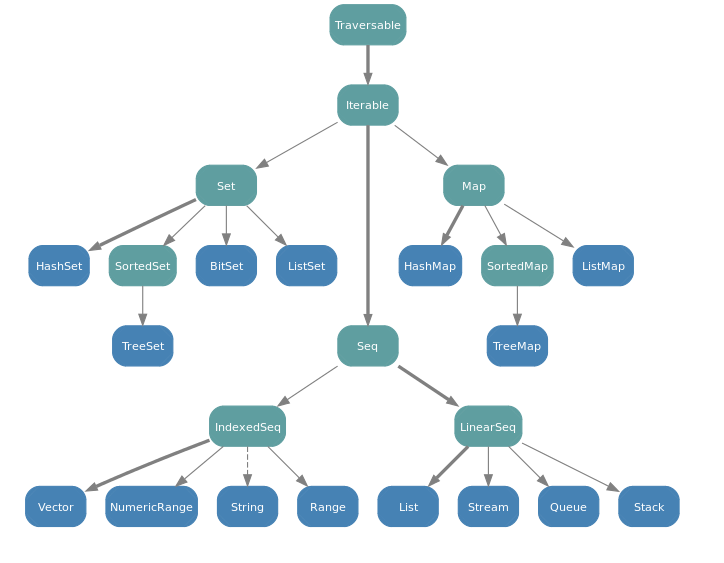
\includegraphics[width=0.82\textwidth]{../img/collection/collection-immutable}
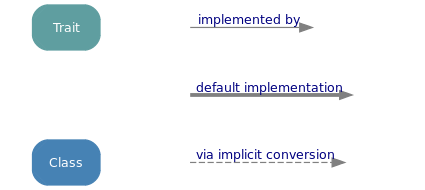
\includegraphics[width=0.33\textwidth]{../img/collection/collection-legend}
\end{Slide}


\begin{Slide}{scala.collection.mutable}
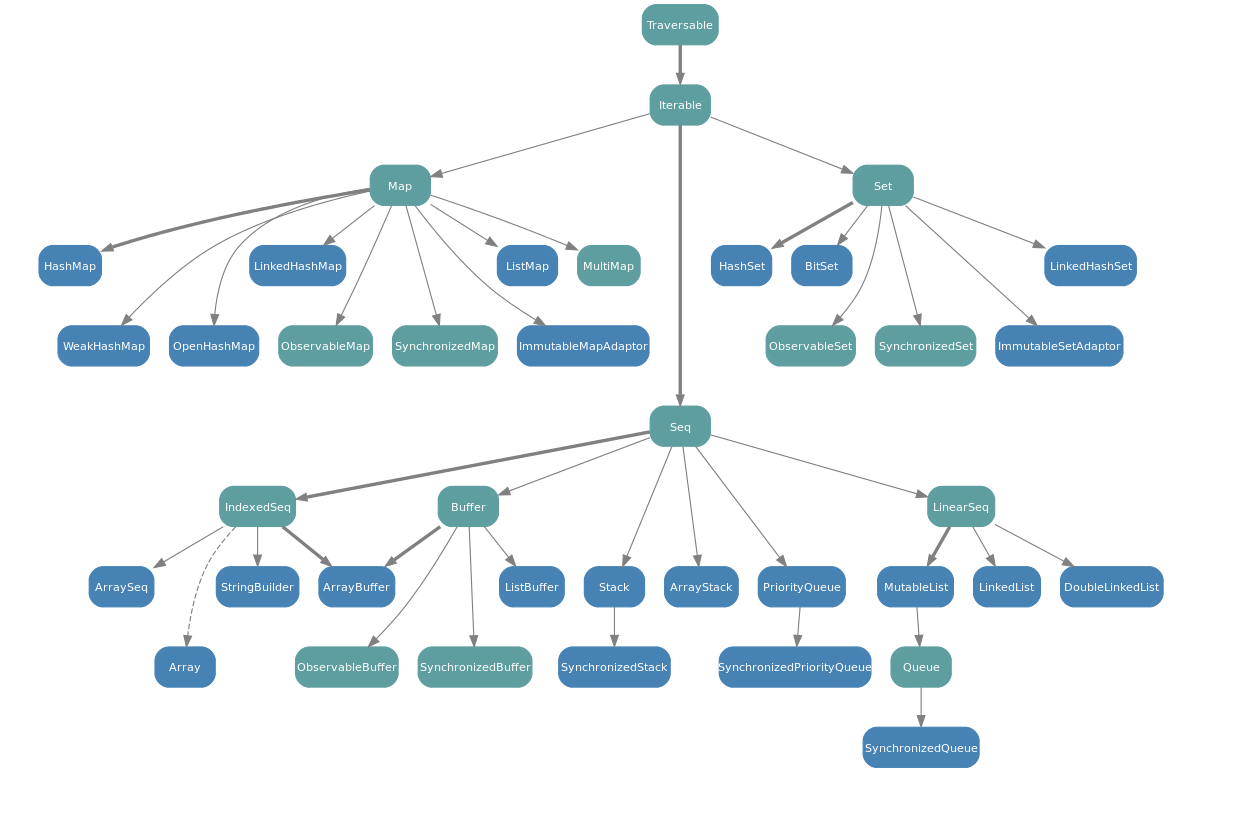
\includegraphics[width=1.05\textwidth]{../img/collection/collection-mutable}
\end{Slide}

\fi

\begin{Slide}{Strängar är implicit en \texttt{IndexedSeq[Char]}}\SlideFontSmall
Det finns en så kallad \Emph{implicit konvertering} mellan \code{String} och \code{IndexedSeq[Char]} vilket gör att \Alert{alla samlingsmetoder på \texttt{Seq} även funkar på strängar} och även flera andra smidiga strängmetoder erbjuds \Alert{utöver} de som finns i \href{http://docs.oracle.com/javase/8/docs/api/java/lang/String.html}{\code{java.lang.String}} genom klassen \href{http://www.scala-lang.org/api/current/scala/collection/immutable/StringOps.html}{\code{StringOps}}.

\vspace{0.5em}
\begin{REPLnonum}
scala> "hej".  //tryck på TAB och se alla strängmetoder
\end{REPLnonum}
Detta är en stor fördel med Scala jämfört med många andra språk, som har strängar som inte kan allt som andra sekvenssamlingar kan.
\end{Slide}


% \begin{Slide}{\texttt{Vector} eller \texttt{List}?}\SlideFontTiny
% {\href{http://stackoverflow.com/questions/6928327/when-should-i-choose-vector-in-scala}{stackoverflow.com/questions/6928327/when-should-i-choose-vector-in-scala}}
%
% \begin{enumerate}
% \item If we only need to transform sequences by operations like map, filter, fold etc: basically it does not matter, we should program our algorithm generically and might even benefit from accepting parallel sequences. For sequential operations List is probably a bit faster. But you should benchmark it if you have to optimize.
%
% \item If we need a lot of random access and different updates, so we should use vector, list will be prohibitively slow.
%
% \item If we operate on lists in a classical functional way, building them by prepending and iterating by recursive decomposition: use list, vector will be slower by a factor 10-100 or more.
%
% \item If we have an performance critical algorithm that is basically imperative and does a lot of random access on a list, something like in place quick-sort: use an imperative data structure, e.g. ArrayBuffer, locally and copy your data from and to it.
% \end{enumerate}
% {\href{http://stackoverflow.com/questions/20612729/how-does-scalas-vector-work}{stackoverflow.com/questions/20612729/how-does-scalas-vector-work}}\\
% Mer om tids- och minneskomplexitet i fördjupningskursen och senare kurser.
% \end{Slide}




\begin{Slide}{Speciella metoder på förändringsbara samlingar}\SlideFontSmall
Både \code{Set} och \code{Map} finns i \Alert{förändringsbara} varianter med extra metoder för uppdatering av innehållet ''på plats'' utan att nya samlingar skapas.
\begin{REPL}
scala> import scala.collection.mutable

scala> val ms = mutable.Set.empty[Int]
ms: scala.collection.mutable.Set[Int] = Set()

scala> ms += 42
res0: ms.type = Set(42)

scala> ms += (1, 2, 3, 1, 2, 3); ms -= 1
res1: ms.type = Set(2, 42, 3)

scala> ms.mkString("Mängd: ", ", ", " Antal: " + ms.size)
res2: String = Mängd: 1, 2, 42, 3 Antal: 4

scala> val ordpar = mutable.Map.empty[String, String]
scala> ordpar += ("hej" -> "svejs", "abra" -> "kadabra", "ada" -> "lovelace")
scala> println(ordpar("abra"))
kadabra
\end{REPL}
\end{Slide}

\begin{Slide}{Fler exempel på samlingsmetoder}
Exempel att öva på: räkna bokstäver i ord.  \\
Undersök vad som händer i REPL:
\begin{Code}[basicstyle=\SlideFontSize{9}{13}\ttfamily]
val ord = "sex laxar i en laxask sju sjösjuka sjömän"
val uppdelad = ord.split(' ').toVector
val ordlängd = uppdelad.map(_.length)
val ordlängdMap = uppdelad.map(s => (s, s.size)).toMap
val grupperaEfterFörstaBokstav = uppdelad.groupBy(s => s(0))
val bokstäver = ord.toVector.filter(_ != ' ')
val antalX = bokstäver.count(_ == 'x')
val grupperade = bokstäver.groupBy(ch => ch)
val antal = grupperade.mapValues(_.size)
val sorterat = antal.toVector.sortBy(_._2)
val vanligast = antal.maxBy(_._2)
\end{Code}
\end{Slide}


\begin{Slide}{Föränderlig lokalt, returnera oföränderlig}
\SlideFontSmall
Om du vill implementera en imperativ algoritm med en föränderlig samling:\\
Gör gärna detta \Alert{lokalt} i en \Alert{förändringsbar} samling och returnera sedan en \Emph{oföränderlig} samling, genom att köra t.ex. \code{toSet} på en mängd, eller \code{toMap} på en hashtabell, eller \code{toVector} på en \code{ArrayBuffer} eller \code{Array}.

\begin{REPL}
scala> :paste
def kastaTärningTillsAllaUtfallUtomEtt(sidor: Int = 6) = {
  val s = scala.collection.mutable.Set.empty[Int]
  var n = 0
  while (s.size < sidor - 1) {
    s += (math.random * sidor + 1).toInt
    n += 1
  }
  (n, s.toSet)
}
scala> kastaTärningTillsAllaUtfallUtomEtt()
res0: (Int, scala.collection.immutable.Set[Int]) = (13,Set(5, 1, 6, 2, 3))

\end{REPL}
\end{Slide}


\begin{Slide}{Metoden \texttt{sliding}}\SlideFontSmall
Metoden \code{sliding(n)} skapar med ett ''glidande fönster'' en sekvens av
delsekvenser av längd \code{n} genom att ''svepa fönstret'' från början till slut:
\begin{REPL}
scala> val xs = "fem myror är fler än fyra elefanter".split(' ').toVector
xs: Vector[String] = Vector(fem, myror, är, fler, än, fyra, elefanter)

scala> xs.sliding(2).toVector
res0: Vector[Vector[String]] =
  Vector(Vector(fem, myror), Vector(myror, är), Vector(är, fler),
     Vector(fler, än), Vector(än, fyra), Vector(fyra, elefanter))

scala> xs.sliding(3).toVector
res1: Vector[Vector[String]] =
  Vector(Vector(fem, myror, är), Vector(myror, är, fler),
    Vector(är, fler, än), Vector(fler, än, fyra),
      Vector(än, fyra, elefanter))
\end{REPL}
Denna metod har du nytta av på veckans laboration!
\\(se fler exempel på övning)
\end{Slide}

%!TEX encoding = UTF-8 Unicode
%!TEX root = ../lect-w09.tex


\Subsection{Serialisering och deserialisering}

\begin{Slide}{Serialisering och deserialisering}
\begin{itemize}
  \item Att \Emph{serialisera} innebär att \Alert{koda objekt} i minnet till en avkodningsbar \Alert{sekvens av symboler}, som kan lagras t.ex. i en fil på din hårddisk.
  \item Att \Emph{de-serialisera} innebär att \Alert{avkoda en sekvens av symboler}, t.ex. från en fil, och \Alert{återskapa objekt} i minnet.
\end{itemize}
\end{Slide}


\begin{Slide}{Läsa text från fil och URL}
I paketet \code{scala.io} finns singelobjektet \code{Source} med metoderna \code{fromFile} och \code{fromUrl} för läsning från fil resp. från  URL\footnote{URL = Universal Resource Locator}, som börjar t.ex. med \code{http://}
\begin{Code}
def läsFrånFil(filnamn: String) = scala.io.Source.fromFile(filnamn).mkString

def läsRaderFrånFil(filnamn: String): Vector[String] =
  scala.io.Source.fromFile(filnamn).getLines.toVector

def läsFrånWebbsida(url: String) = scala.io.Source.fromURL(url).mkString

def läsRaderWebbsida(url: String, kodning: String = "UTF-8"): Vector[String] =
  scala.io.Source.fromURL(url, kodning).getLines.toVector

\end{Code}
Se exempel på veckans övning.
\end{Slide}


\begin{Slide}{Serialisering i modulen \texttt{introprog.IO}}
  \begin{itemize}
    \item I kursens kodbibliotek \code{introprog} finns ett singelobjekt \code{IO} som samlar smidiga funktioner för serialisering och de-serialisering. 
    \item Se api-dokumentation här: \\ \url{http://cs.lth.se/pgk/api/} \\ Sök på IO och klicka på singelobjektet.
    \item Se koden här:\\
    \url{https://github.com/lunduniversity/introprog-scalalib/blob/master/src/main/scala/introprog/IO.scala}
    \item Om du vill får du gärna använda \code{introprog.IO} istället för \code{scala.io.Source} på labben.  
  \end{itemize}
\end{Slide}

%%!TEX encoding = UTF-8 Unicode
%!TEX root = ../lect-w09.tex

\ifkompendium\else
\Subsection{Grumligtlådan}

\begin{Slide}{Grumligtlådan: topplista med ämnen 2017}
\begin{multicols}{2}
\begin{verbatim}
  om kursen       : 14
  klass           : 9
  this            : 7
  filstruktur     : 5
  pluggteknik     : 4
  case-klass      : 4
  registrera      : 3
  filtrera        : 3
  copy            : 3
  tupel           : 2
  konstruktor     : 2
  iterera         : 2
  fabriksmetod    : 2
  synlighet       : 1
  skuggning       : 1
  sidoeffekt      : 1
  Seq[T]          : 1
  sekvenser       : 1
  sats/uttryck    : 1
  lambda          : 1
  kompanjonsobj   : 1
  högre ordn funk : 1
  funktion        : 1
  curry-funktion  : 1
\end{verbatim}
\end{multicols}
\end{Slide}



\begin{Slide}{Grumligtlådan: lajvkodning}
Lajvkodning enligt begrepp i lådan utifrån denna klass:
\begin{Code}[basicstyle=\ttfamily\SlideFontSize{12}{14}]
class Frog(var n: Int) { def hop = n += 1 }
\end{Code}

\includegraphics[width=0.6\textwidth]{../img/frog}
\end{Slide}

\fi


%\chapter{Matriser}
\begin{itemize}[nosep]
\item matriser
\item nästlade for-satser
\item designexempel: Tre-i-rad
\item matriser i Java vs Scala\end{itemize}
%!TEX encoding = UTF-8 Unicode
%!TEX root = ../exercises.tex

\ifPreSolution


\Exercise{\ExeWeekNINE}\label{exe:W09}

\begin{Goals}
%!TEX encoding = UTF-8 Unicode
%!TEX root = ../compendium2.tex

%\item Kunna skapa och använda tupler, som variabelvärden, parametrar och returvärden.

%\item Förstå skillnaden mellan ett objekt och en klass och kunna förklara betydelsen av begreppet instans.

%\item Kunna skapa och använda attribut som medlemmar i objekt och klasser och som som klassparametrar.

%\item Kunna beskriva den praktiska nyttan med att ett attribut är privat.

%\item Kunna byta ut implementationen av metoden \code{toString}.

%\item Kunna skapa och använda en objektfabrik med metoden \code{apply}.

%\item Kunna skapa och använda en enkel case-klass.

%\item Kunna använda operatornotation och förklara relationen till punktnotation.

%\item Förstå konsekvensen av uppdatering av föränderlig data i samband med multipla referenser.

%\item Kunna förklara den principiella skillnaderna mellan olika typer av samlingar.
\item Kunna skapa och använda tupler som parametrar och returvärden.
\item Känna till och kunna använda grundläggande metoder på samlingar.
\item Kunna skapa och använda både oföränderliga och föränderliga mängder.
\item Förstå skillnader och likheter mellan en mängd och en sekvens.
\item Kunna beskriva hur algoritmen linjärsökning fungerar.
\item Kunna skapa och använda både oföränderliga och föränderliga nyckel-värde-tabeller.
\item Kunna använda nyckel-värde-tabeller för att implementera registrering.
\item Förstå likheter och skillnader mellan en nyckel-värde-tabell och en sekvens.
\item Kunna spara och läsa data till/från textfiler på disk.
 
\end{Goals}

\begin{Preparations}
\item \StudyTheory{09}
\end{Preparations}

\else

\ExerciseSolution{\ExeWeekNINE}

\fi



\BasicTasks %%%%%%%%%%%%%%%%




\WHAT{Para ihop begrepp med beskrivning.}

\QUESTBEGIN

\Task \what

\vspace{1em}\noindent Koppla varje begrepp med den (förenklade) beskrivning som passar bäst:

\begin{ConceptConnections}
  bastyp & 1 & & A & körtidstypen avgör vilken metod som körs \\ 
  supertyp & 2 & & B & minneslagring kan optimeras, har supertypen \code|AnyVal| \\ 
  subtyp & 3 & & C & klass utan namn, utvidgad med extra implementation \\ 
  körtidstyp & 4 & & D & är endast synlig i subtyper \\ 
  dynamisk bindning & 5 & & E & kan ej instansieras \\ 
  polymorfism & 6 & & F & abstrakt klass, kan mixas in, kan ej ha parametrar \\ 
  trait & 7 & & G & saknar implementation \\ 
  inmixning & 8 & & H & kan vara mer specifik än den statiska typen \\ 
  överskuggad medlem & 9 & & I & ej värdetyp, har supertypen \code|AnyRef| \\ 
  anonym klass & 10 & & J & kan ha många former, t.ex. en av flera subtyper \\ 
  skyddad medlem & 11 & & K & subtypning utanför denna kodfil är förhindrad \\ 
  abstrakt medlem & 12 & & L & medlem i subtyp ersätter medlem i supertyp \\ 
  abstrakt klass & 13 & & M & en typ som är mer specifik \\ 
  referenstyp & 14 & & N & en typ som är mer generell \\ 
  förseglad typ & 15 & & O & klass får nya egenskaper från trait \\ 
  värdetyp & 16 & & P & den mest generella typen i en arvshierarki \\ 
\end{ConceptConnections}

\SOLUTION

\TaskSolved \what

\begin{ConceptConnections}
  bastyp & 1 & ~~\Large$\leadsto$~~ &  P & den mest generella typen i en arvshierarki \\ 
  sypertyp & 2 & ~~\Large$\leadsto$~~ &  N & en typ som är mer generell \\ 
  subtyp & 3 & ~~\Large$\leadsto$~~ &  M & en typ som är mer specifik \\ 
  körtidstyp & 4 & ~~\Large$\leadsto$~~ &  H & kan vara mer specifik än den statiska typen \\ 
  dynamisk bindning & 5 & ~~\Large$\leadsto$~~ &  A & körtidstypen avgör vilken metod som körs \\ 
  plymorfism & 6 & ~~\Large$\leadsto$~~ &  J & kan ha många former, t.ex. en av flera subtyper \\ 
  trait & 7 & ~~\Large$\leadsto$~~ &  F & abstrakt klass, kan mixas in, kan ej ha parametrar \\ 
  inmixning & 8 & ~~\Large$\leadsto$~~ &  O & klass får nya egenskaper från trait \\ 
  överskuggad medlem & 9 & ~~\Large$\leadsto$~~ &  L & medlem i subtyp ersätter medlem i supertyp \\ 
  anonym klass & 10 & ~~\Large$\leadsto$~~ &  C & den mest generella typen i en arvshierarki \\ 
  skyddad medlem & 11 & ~~\Large$\leadsto$~~ &  D & är endast synlig i subtyper \\ 
  abstrakt medlem & 12 & ~~\Large$\leadsto$~~ &  G & saknar implementation \\ 
  abstrakt klass & 13 & ~~\Large$\leadsto$~~ &  E & kan ej instansieras \\ 
  referenstyp & 14 & ~~\Large$\leadsto$~~ &  I & ej värdetyp, har supertypen \code|AnyRef| \\ 
  förseglad typ & 15 & ~~\Large$\leadsto$~~ &  K & subtypning utanför denna kodfil är förhindrad \\ 
  värdetyp & 16 & ~~\Large$\leadsto$~~ &  B & minneslagring kan optimeras, har supertypen, \code|AnyVal| \\ 
\end{ConceptConnections}

\QUESTEND



\WHAT{Vad är en mängd?}
\QUESTBEGIN

\Task \what~ Förklara vad som händer nedan. Varför hamnar elementen i en ''konstig'' ordning? Varför ''försvinner'' det element?

\begin{REPL}
scala> val xs = Vector(1,2,3,1,2,3,4,5,7).toSet
xs: scala.collection.immutable.Set[Int] = Set(5, 1, 2, 7, 3, 4)
scala> xs.foreach(print)
512734
\end{REPL}

\SOLUTION

\TaskSolved \what~En mängd är en samling som snabbt kan ge svaret på frågan om ett visst element ingår i samlingen eller ej. Elementen i en mängd är unika. Tilläg av redan existerande element ignoreras. En mängd är inte en  sekvens, eftersom traversering med t.ex. \code{map} eller \code{foreach} inte (nödvändigtvis) sker i den ordning som elementen gavs när mängden konstruerades eller uppdaterades.

\QUESTEND


\WHAT{Använda mängder.}

\QUESTBEGIN

\Task \what

\vspace{1em}\noindent Para ihop varje uttryck till vänster med ett uttryck till höger som har samma värde:

\begin{ConceptConnections}
  \code|Set(1, 2) ++ Set(1, 2)          | & 1 & & A & \code|3             | \\ 
  \code|(1 to 3).toSet                  | & 2 & & B & \code|Set(3)        | \\ 
  \code|Vector.fill(3)(1).toSet         | & 3 & & C & \code|6             | \\ 
  \code|Set(1, 2, 3) diff Set(1, 2)     | & 4 & & D & \code|error: ...    | \\ 
  \code|(1 to 7).toSet.apply(8)         | & 5 & & E & \code|true          | \\ 
  \code|Set(1, 2, 3).sorted             | & 6 & & F & \code|Set(1, 2) - 2 | \\ 
  \code|Set(2,4) subsetOf (1 to 7).toSet| & 7 & & G & \code|Set(1) + 2 + 3| \\ 
  \code|Set(1, -1, 2, -2).map(_.abs).sum| & 8 & & H & \code|false         | \\ 
  \code|Set(1, 1, 1, 1, 1, 5).sum       | & 9 & & I & \code|Set(1, 2)     | \\ 
\end{ConceptConnections}

\SOLUTION

\TaskSolved \what

\begin{ConceptConnections}
  \code|Set(1, 2) ++ Set(1, 2)          | & 1 & ~~\Large$\leadsto$~~ &  I & \code|Set(1, 2)     | \\ 
  \code|(1 to 3).toSet                  | & 2 & ~~\Large$\leadsto$~~ &  G & \code|Set(1) + 2 + 3| \\ 
  \code|Vector.fill(3)(1).toSet         | & 3 & ~~\Large$\leadsto$~~ &  F & \code|Set(1, 2) - 2 | \\ 
  \code|Set(1, 2, 3) diff Set(1, 2)     | & 4 & ~~\Large$\leadsto$~~ &  B & \code|Set(3)        | \\ 
  \code|(1 to 7).toSet.apply(8)         | & 5 & ~~\Large$\leadsto$~~ &  H & \code|false         | \\ 
  \code|Set(1, 2, 3).sorted             | & 6 & ~~\Large$\leadsto$~~ &  D & \code|error: ...    | \\ 
  \code|Set(2,4) subsetOf (1 to 7).toSet| & 7 & ~~\Large$\leadsto$~~ &  E & \code|true          | \\ 
  \code|Set(1, -1, 2, -2).map(_.abs).sum| & 8 & ~~\Large$\leadsto$~~ &  A & \code|3             | \\ 
  \code|Set(1, 1, 1, 1, 1, 5).sum       | & 9 & ~~\Large$\leadsto$~~ &  C & \code|6             | \\ 
\end{ConceptConnections}

\QUESTEND


\WHAT{Räkna unika ord med hjälp av en mängd.}

\QUESTBEGIN

\Task \what~På veckans laboration ska vi göra automatisk språkbehandling av långa texter som vi delar upp i ord. Med metoden \code{s.split(' ').toVector} kan du dela upp en sträng \code{s} i en sekvens av ord, där \code{s} blivit uppdelad i många strängar vid varje blanktecken och alla blanktecken är borttagna.

\Subtask Använd metoderna \code{split} och \code{toSet} för skapa ett uttryck som beräknar hur många unika ord det finns i strängen \code{hej} nedan:
\begin{REPLnonum}
scala> val hej = "hej hej hemskt mycket hej"
\end{REPLnonum}

\Subtask Mängder är snabba på att kolla om ett element finns i mängden men du kan inte förvänta dig att elementen finns i någon viss ordning. Det finns en sekvenssamlingsmetod som skapar en sekvens med unika element ur en sekvens och behåller den ursprungliga ordningen. Vad heter metoden? \\\emph{Tips:} Leta i snabbreferensen eller sök på nätet. Metoden fungerar på alla samlingar som är av typen \code{Seq} och har ett namn som börjar med bokstäverna \code{di}.

\SOLUTION

\TaskSolved \what~

\SubtaskSolved
\begin{REPL}
scala> val hej = "hej hej hemskt mycket hej"
scala> val n = hej.split(' ').toSet.size
n: Int = 3
\end{REPL}

\SubtaskSolved Metoden \code{distinct} returnerar en sekvens med unika element och bibehållen ursprunglig ordning.

\QUESTEND




\WHAT{Skapa 2-tupler med metoden \code{->} som kan uttalas ''mappas till''.}

\QUESTBEGIN

\Task \what~Vi har tidigare sett hur två olika värden kan samlas i en 2-tupel, till exempel \code{(0, true)}. Par kan även skapas med hjälp av metoden \code{->} enligt nedan. Testa detta i REPL:
\begin{REPL}
scala> ("Skåne", "Lund")          // ett strängpar med vanlig 2-tupel
scala> "Skåne" -> "Lund"           // operatornotation med ->
scala> "Skåne".->("Lund")         // punktnotation med -> (inte alls vanligt)
\end{REPL}
Metoden \code{->} fungerar med alla typer och är en fabriksmetod för par. Metodnamnet liknar en högerpil och illustrerar en mappning från första till andra värdet.

\Subtask Fungerar det på par skapade med \code{->} att använda metoderna \code{_1} och \code{_2}?


\Subtask Deklarera en variabel \code{val huvudstad: Vector[(String, String)]} som innehåller mappningar mellan geografiska områden och deras huvudstäder enligt tabellen nedan.

\begin{table}[H]
  \renewcommand{\arraystretch}{1.2}
  \begin{tabular}{|l|l|}\hline
  Sverige & Stockholm \\\hline
  Danmark & Köpenhamn \\\hline
  Grönland & Nuuk \\\hline
  Skåne & Lund \\\hline
  \end{tabular}
\end{table}

\Subtask Skriv ett uttryck som plockar fram \code{"Lund"} ur \code{huvudstad}.

\SOLUTION


\TaskSolved \what

\SubtaskSolved Ja, fabriksmetoden returnerar ett helt vanligt par:
\begin{REPLnonum}
scala> val härBorJag = "Skåne" -> "Lund"
val härBorJag: (String, String) = (Skåne,Lund)

scala> härBorJag._1
val res0: String = Skåne

scala> härBorJag._2
val res1: String = Lund
\end{REPLnonum}


\SubtaskSolved

\begin{Code}
val huvudstad = Vector(
  "Sverige"  -> "Stockholm",
  "Danmark"  -> "Köpenhamn",
  "Grönland" -> "Nuuk",
  "Skåne"    -> "Lund"
)
\end{Code}

\SubtaskSolved
\begin{REPL}
scala> huvudstad(3)._2
val res2: String = Lund
\end{REPL}

\QUESTEND



\WHAT{Linjärsöka efter nyckel i sekvens av mappningar.}

\QUESTBEGIN

\Task \what~

\Subtask Implementera funktionen \code{lookupIndex} nedan med hjälp av samlingsmetoden \code{indexWhere} så att linjärsökning sker efter index för ett par i sekvensen där \code{key} finns på första platsen i paret.

\begin{Code}
def lookupIndex(xs: Vector[(String, String)])(key: String): Int = ???
\end{Code}

\Subtask Testa din funktion i REPL genom att slå upp index för Skånes huvudstad i sekvensen \code{huvudstad} från föregående uppgift.

\SOLUTION

\TaskSolved \what~

\SubtaskSolved
\begin{Code}
def lookupIndex(xs: Vector[(String, String)])(key: String): Int =
  xs.indexWhere(_._1 == key)
\end{Code}

\SubtaskSolved
\begin{REPL}
scala> val i = lookupIndex(huvudstad)("Skåne")
val i: Int = 3

scala> huvudstad(i)._2
val res2: String = Lund
\end{REPL}

\noindent Eller med funktioner som återanvändbara dellösningar:
\begin{REPL}
scala> val indexOf = lookupIndex(huvudstad) _

scala> def capital(key: String) = huvudstad(indexOf(key))._2

scala> capital("Skåne")
val res3: String = Lund

scala> capital("Sverige")
val res4: String = Stockholm
\end{REPL}

\QUESTEND



\WHAT{Nyckel-värde-tabell.}

\QUESTBEGIN

\Task \what~En nyckel-värde-tabell är en smart datastruktur som gör att du kan slå upp det värde som en nyckel mappar till \emph{utan} att linjärsökning behöver ske. Värdet plockas fram direkt på en konstant tid, d.v.s. tiden att slå upp ett värde beror \emph{inte} på antalet element i samlingen, utan sker med mycket liten fördröjning.

I Scala heter nyckelvärdetabeller \code{Map} med stort M och är praktiska att använda i många olika sammanhang. \code{Map} finns i både en oföränderlig och en förändringsbar variant. Det går med metoder på formen \code{toXXX} lätt att omvandla mellan en \code{Map} och en sekvens av par av typen \code{XXX[(Nyckeltyp, Värdetyp)]}.

\Subtask Deklarera mappen \code{telnr} nedan i REPL och använd \code{apply} för att ta reda på telefonnumret till Fröken Ur.

\Subtask Vad har \code{telnr} för typ?

\Subtask Vad har \code{telnr.toVector} för typ?

\begin{Code}
val telnr = Map(
  "Anna"     -> 46462229812L,
  "Björn"     -> 46462229009L,
  "Sandra"    -> 46462220368L,
  "Fröken Ur" -> 4690510L,
)
\end{Code}
En uppsättning \code{Map}-instanser, vid behov nästlade, kan med fördel användas för att bygga upp en i-minnet-databas där inbyggda samlingsmetoder, t.ex. \code{map}, \code{filter}, och \code{for}-\code{yield}-uttryck, ger flexibla och effektiva sökmöjligheter. På veckans laboration ska du göra detta.

Samlingen \code{Map} är en generalisering av en sekvens, där man kan ''indexera'', inte bara med ett heltal, utan med vilken typ av värde som helst, t.ex. en sträng. Datastrukturen \code{Map} kallas också \emph{associativ array}\footnote{\href{https://en.wikipedia.org/wiki/Associative_array}{https://en.wikipedia.org/wiki/Associative\_array}} och är implementerad som en s.k. \emph{hashtabell}\footnote{\href{https://en.wikipedia.org/wiki/Hash_table}{https://en.wikipedia.org/wiki/Hash\_table}}, men du får vänta till fördjupningskursen innan vi går igenom hur en sådan datastruktur implementeras.

\SOLUTION

\TaskSolved \what~

\begin{REPL}
scala> telnr("Fröken Ur")
val res0: Long = 464690510

scala> :type telnr
Map[String,Long]

scala> :type telnr.toVector
Vector[(String, Long)]
\end{REPL}

\QUESTEND



\WHAT{Använda nyckel-värdetabell.}

\QUESTBEGIN

\Task \what~

\Subtask Skapa nedan variabler i REPL.
\begin{Code}
val follow = for i <- 2 to 16 by 2 yield (i, i + 1)
val xs = follow.toMap
val ys = xs.toVector
\end{Code}
Hamnar mappningarna i \code{ys} i samma ordning som \code{follow}? Varför?

\Subtask Med \code{xs} och \code{ys} deklarerade i REPL enligt ovan, para ihop yttryck till vänster med rätt resultat till höger. Om du är osäker på de sammansatta uttrycken, prova enklare uttryck i REPL och undersök värde och typ hos delresultat.

\begin{ConceptConnections}
  \code|xs(2) + xs(4)                 | & 1 & & A & \code|1                     | \\ 
  \code|ys(2) + ys(4)                 | & 2 & & B & \code|false                 | \\ 
  \code|ys(0)                         | & 3 & & C & \code|8                     | \\ 
  \code|xs(0)                         | & 4 & & D & \code|(16, 17)              | \\ 
  \code|(xs + (0 -> 1)).apply(0)      | & 5 & & E & \code|NoSuchElementException| \\ 
  \code|xs.keySet.apply(2)            | & 6 & & F & \code|(10, 11)              | \\ 
  \code|xs isDefinedAt 0              | & 7 & & G & \code|7                     | \\ 
  \code|xs.getOrElse(0, 7)            | & 8 & & H & \verb|error: type mismatch  | \\ 
  \code|xs.maxBy(_._2)                | & 9 & & I & \code|-9                    | \\ 
  \code|xs.map(p => p._1 -> -p._2)(8) | & 10 & & J & \code|true                  | \\ 
\end{ConceptConnections}

\SOLUTION

\TaskSolved \what


\SubtaskSolved Nej nyckel-värde-paren lagras i någon speciell ordning som bestäms av en intern, smart lagringsprincip enligt en s.k. hashfunktion\footnote{\url{https://sv.wikipedia.org/wiki/Hashfunktion}}, för att åstadkomma snabba uppslagningar av värden från nycklar och vilket normalt inte sammanfaller med ordningen i den sekvens som de skapades ur.

\SubtaskSolved

\begin{ConceptConnections}
    \code|xs(2) + xs(4)                 | & 1 & ~~\Large$\leadsto$~~ &  A & \code|8                     | \\ 
  \code|ys(0)                         | & 2 & ~~\Large$\leadsto$~~ &  C & \code|(10, 11)              | \\ 
  \code|xs(0)                         | & 3 & ~~\Large$\leadsto$~~ &  I & \code|NoSuchElementException| \\ 
  \code|(xs + (0 -> 1)).apply(0)      | & 4 & ~~\Large$\leadsto$~~ &  D & \code|1                     | \\ 
  \code|xs.keySet.apply(2)            | & 5 & ~~\Large$\leadsto$~~ &  G & \code|true                  | \\ 
  \code|xs isDefinedAt 0              | & 6 & ~~\Large$\leadsto$~~ &  H & \code|false                 | \\ 
  \code|xs.getOrElse(0, 7)            | & 7 & ~~\Large$\leadsto$~~ &  B & \code|7                     | \\ 
  \code|xs.maxBy(_._2)                | & 8 & ~~\Large$\leadsto$~~ &  E & \code|(16, 17)              | \\ 
  \code|xs.map(p => p._1 -> -p._2)(8) | & 9 & ~~\Large$\leadsto$~~ &  F & \code|-9                    | \\ 
\end{ConceptConnections}

%%% BELOW IS SOLVED IN SCALA 3 AND the err msg is better! :)
% \noindent \emph{Fördjupning}:  Felmeddelandet som rad 2 ovan orsakar är lurigt:

% \begin{REPL}
% scala> ys(2)
% val res22: (Int, Int) = (6,7)

% scala> ys(4)
% val res23: (Int, Int) = (12,13)

% scala> ys(2) + ys(4)
% <console>:13: error: type mismatch;
%  found   : (Int, Int)
%  required: String
%        ys(2) + ys(4)

% \end{REPL}
% Det går som förväntat inte att addera två tupler, men varför säger kompilatorn att en sträng krävs?!? Detta beror på att, i enlighet med hur det fungerar i Java, valde Scala-språkets konstruktörer att låta strängsammanfogning fungera med alla möjliga typer vilket gör att kompilatorn inte ger upp när metoden \code{+} inte finns för tupler, utan i stället gör ett misslyckat försök med strängsammanfogning.

% Det mest olyckliga med detta är inte att felmeddelanden ibland blir missvisande, utan att det i vissa situationer inte ens \emph{blir} något felmeddelande, trots att man av rent misstag råkat strängkonkatenera i stället för t.ex. lägga till ett element i en mängd eller en mappning i en tabell. Detta typosäkra beteendet av strängsammanfogning har kritiserats, men det är inte okontroversiellt att ändra detta nu när så många utvecklare skrivit så mycket Scala-kod som bygger på strängars förmåga att kunna lägga till vad som helst på slutet. Situationen i Scala är dock inte hopplös efter introduktionen av stränginterpolering i Scala 2.10, som möjliggör infogande av värden i strängar på ett typsäkert sätt.
\QUESTEND





\WHAT{Registrering i förändringsbar nyckel-värde-tabell.}

\QUESTBEGIN

\Task \what~I denna uppgift ska du implementera en hjälpklass för registrering i en frekvenstabell som du sedan ska använda på veckans laboration. Klassen ska heta  \code{FreqMapBuilder} som efter upprepade anrop av metoden \code{add(s: String): Unit} kan skapa frekvenstabeller av typen \code{Map[String, Int]}, där nyckel-värde-paren i tabellen anger antalet förekomster av en viss sträng. Du ska utgå från koden nedan.

Klassen använder en förändringsbar tabell internt. Efter att man har lagt till många strängar kan man med metoden \code{toMap} få en oföränderlig tabell för  uppslagning av frekvenser för specifika strängar. Läs i snabbreferensen om vilka extra metoder för uppdatering som erbjuds av \code{mutable.Map[K, V]}.

\begin{Code}
class FreqMapBuilder:
  private val register = collection.mutable.Map.empty[String, Int]
  def toMap: Map[String, Int] = register.toMap
  def add(s: String): Unit = ???

object FreqMapBuilder:
  def apply(xs: String*): FreqMapBuilder = ???
\end{Code}

\noindent Implementera och testa \code{FreqMapBuilder}. \emph{Tips:} Du kan t.ex. använda metoderna \code{+=} och \code{getOrElse}.

\SOLUTION

\TaskSolved \what~
\begin{Code}
class FreqMapBuilder:
  private val register = scala.collection.mutable.Map.empty[String,Int]
  def toMap: Map[String, Int] = register.toMap
  def add(s: String): Unit =
    register += (s -> (register.getOrElse(s, 0) + 1))

object FreqMapBuilder:
  def apply(xs: String*): FreqMapBuilder = 
    val result = new FreqMapBuilder
    xs.foreach(result.add)
    result
\end{Code}

\QUESTEND



\WHAT{Metoden \code{sliding}.}

\QUESTBEGIN

\Task  \what~  I veckans laboration kommer du att ha nytta av metoden \code{sliding}, som ger en iterator för speciella delsekvenser av en sekvens, vilka kan liknas vid ''utsikten'' i ett ''glidande fönster''.

\Subtask Kör nedan i REPL och beskriv vad som händer.

\begin{REPL}
scala> val xs = Vector("fem", "gurkor", "är", "fler", "än", "fyra", "tomater")
scala> xs.sliding(2).toVector
scala> xs.sliding(3).toVector
scala> xs.sliding(10).toVector
\end{REPL}

\Subtask Använd \code{xs.sliding(2)} och omvandla varje element i resultatet till ett par. Gör sedan om sekvensen av par till en nyckel-värde-tabell. Vad kan tabellen användas till?

\SOLUTION

\TaskSolved \what

\SubtaskSolved
\begin{REPL}
scala> val xs = Vector("fem", "gurkor", "är", "fler", "än", "fyra", "tomater")
val xs: Vector[String] =
  Vector(fem, gurkor, är, fler, än, fyra, tomater)

scala> xs.sliding(2).toVector
val res9: Vector[Vector[String]] =
  Vector(Vector(fem, gurkor), Vector(gurkor, är), Vector(är, fler), Vector(fler, än), Vector(än, fyra), Vector(fyra, tomater))

scala> xs.sliding(3).toVector
val res10: Vector[Vector[String]] =
  Vector(Vector(fem, gurkor, är), Vector(gurkor, är, fler), Vector(är, fler, än), Vector(fler, än, fyra), Vector(än, fyra, tomater))

scala> xs.sliding(10).toVector
val res11: Vector[Vector[String]] =
  Vector(Vector(fem, gurkor, är, fler, än, fyra, tomater))

\end{REPL}
\code{xs.sliding(n).toVector} skapar en sekvens som innehåller sekvenser av längden \code{n} som bildas genom att ta varje element och dess \code{n - 1} efterföljande element.

\SubtaskSolved
\begin{REPL}
scala> xs.sliding(2).map(ys => ys(0) -> ys(1)).toMap
val res0: Map[String,String] =
  Map(är -> fler,
      än -> fyra,
      fyra -> tomater,
      gurkor -> är,
      fem -> gurkor,
      fler -> än
  )
\end{REPL}
Man kan använda tabellen till att slå upp vilket som är efterföljande ord. Det fungerar eftersom alla ord är unika. Om det funnits flera likadana ord med olika efterföljande ord så hade vi behövt skapa en tabell med nycklar som mappar till en samling som registrerar efterföljande ord. Detta ska vi göra på veckans laboration.

\QUESTEND




\WHAT{Läsa text från fil och webbservrar.}

\QUESTBEGIN

\Task \what~På laborationen ska du bygga upp tabeller från data i textformat. Då har du nytta av att kunna läsa text från filer och från webben. Testa detta i REPL:
\begin{REPL}
scala> val url = "https://fileadmin.cs.lth.se/pgk/europa.txt"
scala> val xs = io.Source.fromURL(url, "UTF-8").getLines.toVector
scala> val data = xs.map(_.split(';').toVector)
scala> data.head
scala> data.foreach(println)
\end{REPL}

\Subtask Skapa dessa tabeller ur sekvensen \code{data}:
\begin{Code}
val populationOf: Map[String, Int]    = ???  // länders invånarantal
val sizeOf:       Map[String, Int]    = ???  // länders yta i km^2
val capitalOf:    Map[String, String] = ???  // länders huvudstäder
\end{Code}
Testa tabellerna i REPL.

\Subtask Spara ner data i en textfil \code{europa.txt}. Läsa in data från filen med metoden\\ \code{Source.fromFile(filnamn, teckenkodning)} på liknande sätt som med  \code{fromURL} ovan. Om du kör i en Linux-terminal kan du enkelt ladda ner en fil så här (notera att det är stora bokstaven \code{O} och inte en nolla i optionen \code{-sLO}):
\begin{REPLnonum}
> curl -sLO https://fileadmin.cs.lth.se/pgk/europa.txt
\end{REPLnonum}
Skriv ut alla raderna i \code{europa.txt} med hjälp av \code{Source.fromFile} i REPL.

\SOLUTION

\TaskSolved \what~

\SubtaskSolved
\begin{CodeSmall}
val populationOf = data.tail.map(v => v(0) -> v(1).toInt).toMap
val sizeOf       = data.tail.map(v => v(0) -> v(2).toInt).toMap
val capitalOf    = data.tail.map(v => v(0) -> v(3)).toMap
\end{CodeSmall}

\begin{REPL}
scala> capitalOf("Sverige")
res2: String = Stockholm

scala> populationOf("Sverige")
res3: Int = 9223766

scala> sizeOf("Sverige")
res4: Int = 449964
\end{REPL}

\begin{REPL}
scala> val filename = "europa.txt"
scala> val xs = io.Source.fromFile(filename, "UTF-8").getLines.toVector
scala> val data = xs.map(_.split(';').toVector)
scala> data.map(_.map(_.take(15).padTo(15,' ')).mkString(" ")).foreach(println)
\end{REPL}
\QUESTEND





\ExtraTasks %%%%%%%%%%%%%%%%%%%%%%%%%%%%%%%%%%%%%%%%%%%%%%%%%%%%%%%%%%%%%%%%%%%%

\WHAT{Skapa ett textspel med hjälp av tabeller.}

\QUESTBEGIN

\Task \what~Gör ett enkelt spel för att träna på olika fakta om Europas länder och huvudstäder genom att läsa data från URL:en:\\ \url{https://fileadmin.cs.lth.se/pgk/europa.txt}
\\Där finns text kodad i UTF-8 med följande innehåll (endast de första raderna visas):
\begin{Code}
Land;Invånarantal;Storlek(km^2);Huvudstad
Albanien;3581655;28748;Tirana
Andorra;71201;468;Andorra la Vella
Belgien;10584534;30528;Bryssel
Bosnien-Hercegovina;4590310;51129;Sarajevo
Bulgarien;7385367;110910;Sofia
Cypern;854000;9250;Nicosia
Danmark;5475791;43094;Köpenhamn
Estland;1324333;45226;Tallinn
Finland;5315280;338145;Helsingfors
Frankrike;61538322;551695;Paris
Färöarna;48344;139574;Torshamn
Grekland;10964021;131940;Aten
// ... etcetera för alla Europas länder.
\end{Code}
Låt till exempel användaren svara på slumpvisa frågor av typen:
\begin{itemize}[noitemsep]
  \item Har Andorra fler invånare än Cypern?
  \item Vad heter huvudstaden i Bulgarien?
  \item Har Danmark större yta än Finland?
\end{itemize}
Använd oföränderliga tabeller med lämpliga nycklar och värden. Du kan använda en mängd med länder/huvudstäder som användaren hittills svarat rätt på för att kunna förhindra att dessa återkommer igen.
\SOLUTION

\TaskSolved --

\QUESTEND



\AdvancedTasks %%%%%%%%%%%%%%%%%%%%%%%%%%%%%%%%%%%%%%%%%%%%%%%%%%%%%%%%%%%%%%%%%


\WHAT{Registrering med \code{groupBy}.}

\QUESTBEGIN

\Task \what~Vi ska nu utnyttja ett riktigt listigt trick för att via en enda kodrad implementera registrering med hjälp av samlingsmetoderna \code{groupBy} och \code{map}.

\Subtask Läs om metoden \code{groupBy} i snabbreferensen. Du hittar den under rubriken \emph{''Methods in trait \code{Iterable[A]}''} eftersom \code{groupBy} fungerar på alla samlingar. Testa \code{groupBy} enligt nedan och beskriv vad som händer.

\begin{REPL}
scala> val xs = Vector(1, 1, 2, 2, 4, 4, 4).groupBy(x => x > 2)
scala> val ys = Vector(1, 1, 2, 2, 4, 4, 4).groupBy(x => x)
\end{REPL}

\Subtask Skapa en funktion \code{freq} med nedan funktionshuvud som returnerar en tabell med antalet förekomster av olika heltal i \code{xs}. Testa \code{freq} på en sekvens av 1000 slumpvisa tärningskast och förklara hur funktionen \code{freq} fungerar. \emph{Tips:} Gör först \code{groupBy(???)} och sedan \code{map(???)}.

\begin{Code}
def freq(xs: Vector[Int]): Map[Int, Int] = ???

def kasta(n: Int): Vector[Int] =
  Vector.fill(n)(scala.util.Random.nextInt(6) + 1)
\end{Code}

\SOLUTION

\TaskSolved \what~

\SubtaskSolved Metoden \code{groupBy} skapar en nyckel-värde-tabell där värdena i tabellen är en sekvens med elementen grupperade på ett speciellt sett.
Mer precist:

Resultatet av \code{xs.groupBy(f: K => V)} för en sekvens \code{xs} av typen \code{Vector[K]} blir en tabell av typen \code{Map[V,Vector[K]]} där varje element \code{e} i \code{xs} är grupperade i samma tabellvärde om de lika är enligt \code{f(e)}. Varje grupp får tabellnyckeln \code{f(e)}.

\emph{Listigt trick:} Om man låter funktionen \code{f} vara enhetsfunktionen som avbildar varje element på sig själv, alltså \code{x => x}, så grupperas värdena i samma sekvens om de är lika.

\begin{REPL}
scala> val xs = Vector(1, 1, 2, 2, 4, 4, 4).groupBy(x => x > 2)
val xs: Map[Boolean,Vector[Int]] =
  Map(false -> Vector(1, 1, 2, 2), true -> Vector(4, 4, 4))

scala> val ys = Vector(1, 1, 2, 2, 4, 4, 4).groupBy(x => x)
val ys: Map[Int,Vector[Int]] =
  Map(2 -> Vector(2, 2), 4 -> Vector(4, 4, 4), 1 -> Vector(1, 1))
\end{REPL}


\SubtaskSolved

\begin{Code}
def freq(xs: Vector[Int]): Map[Int, Int] =
  xs.groupBy(x => x).map(p => p._1 -> p._2.size)
\end{Code}
Förklaring: metoden \code{groupBy} skapar en tabell med par \code{k, v} där \code{v} är en sekvens med så många \code{k} som antalet gånger \code{k} förekommer i \code{xs}. Genom att omvandla alla värden \code{p._2} till storleken \code{p._2.size} får vi en frekvenstabell.

\begin{REPL}
scala> freq(kasta(1000))
val res0: Map[Int,Int] = 
  Map(5 -> 163, 1 -> 174, 6 -> 161, 2 -> 169, 3 -> 167, 4 -> 166)

scala> freq(kasta(1000)).toVector.sortBy(_._1).foreach(println)
(1,183)
(2,167)
(3,169)
(4,179)
(5,154)
(6,148)
\end{REPL}

\QUESTEND





\WHAT{Skriva till fil.}

\QUESTBEGIN

\Task \what~Som hjälp när du skapar egna intressanta applikationer eller bygger vidare på kursens laborationer och övningar med frivilliga extrauppgifter, kan du använda funktionerna i singelobjektet \code{IO} nedan, som finns i kursens scala-bibliotek \href{http://cs.lth.se/pgk/api}{introprog}.\footnote{Källkoden finns här och även på sidan \pageref{disk-access-code}:\\ \href{https://github.com/lunduniversity/introprog/blob/master/compendium/workspace/introprog/src/main/scala/introprog/IO.scala}{https://github.com/lunduniversity/introprog-scalalib/blob/master/src/main/scala/introprog/IO.scala}}

IO-modulen använder \code{scala.io.Source} för att serialisera och de-serialisera strängar till och från vanliga textfiler. IO-modulen använder även paketet \code{java.io} för att erbjuda funktioner som gör det enkelt att serialisera/de-serialisera godtyckliga objekt skapade med hjälp av serialserbara klasser till/från binärfiler. Case-klasser i Scala blir automatiskt serialiserbara.

I implementationen av \code{IO} används \code{try ... finally} för att säkerställa att filer inte lämnas öppnade även om något går fel under den läs/skriv-process som sköts av det underliggande operativsystemet.

\Subtask
Kompilera och resta nedan med \code{introprog} på classpath, t.ex. med hjälp av \code{sbt}.
\begin{Code}
import introprog.IO

case class Player(name: String)

@main def run(): Unit = 
  println("Test of output/input objects to/from disk:")
  val highscores = Map(Player("Sandra") -> 42, Player("Björn") -> 5)
  IO.saveObject(highscores,"highscores.ser")
  val highscores2 = IO.loadObject[Map[Player, Int]]("highscores.ser")
  val isSameContents = highscores2 == highscores
  val testResult = if (isSameContents) "SUCCESS :)" else "FAILURE :("
  println(testResult)
\end{Code}

\Subtask
Använd \code{IO}-modulen för att spara användarens poängresultat i ditt spel om Europas länder och städer, i extrauppgiften ovan. Implementationen av \code{introprog.IO} finns här: \url{https://github.com/lunduniversity/introprog-scalalib/blob/master/src/main/scala/introprog/IO.scala} 

% \begin{figure}
% %  \scalainputlisting[basicstyle=\ttfamily\fontsize{9.2}{11}\selectfont]{examples/IO.scala}
%   \scalainputlisting[basicstyle=\ttfamily\fontsize{9.2}{11}\selectfont]{../workspace/introprog/src/main/scala/introprog/IO.scala}
%   \label{disk-access-code}
% \end{figure}
\SOLUTION

\TaskSolved --

\QUESTEND



%
%
% \subsection{\TODO Värdera nedan gamla uppgifter}
%
%
%
% \WHAT{Objekt med attribut (fält).}
%
% \QUESTBEGIN
%
% \Task  \what~  Ett objekt kan samla data som hör ihop och på så sätt skapa en datastruktur. Data i ett objekt kallas \emph{attribut} eller \emph{fält}, \Eng{field}. Objekt som samlar enbart data kallas även \emph{post} \Eng{record}.
% \begin{REPLnonum}
% scala> object mittKonto { var saldo = 0; val nummer = 12345L }
% \end{REPLnonum}
% \Subtask Skriv en sats som sätter in ett slumpmässigt belopp mellan 0 och en miljon på \code{mittKonto} ovan med hjälp av punktnotation och tilldelning.
%
% \Subtask Vad händer om du försöker ändra attributet \code{nummer}?
%
% \SOLUTION
%
%
% \TaskSolved \what
%
%
% \SubtaskSolved   \code{mittKonto.saldo = (math.random() * 1000000).toInt}
%
% \SubtaskSolved   Går ej eftersom val är oföränderlig, man får alltså ett Error.
%
%
% \QUESTEND
%
%
%
%
% %%<AUTOEXTRACTED by mergesolu>%%      %Uppgift 2
%
%
%
%
% \WHAT{Klass med attribut.}
%
% \QUESTBEGIN
%
% \Task  \what~  Om du vill ha många objekt av samma typ, kan du använda en \textbf{klass}. På så sätt kan man skapa många datastrukturer av samma typ men med olika innehåll. Man skapar nya objekt med nyckelordet \code{new} följt av klassens namn. Klassen utgör en ''mall'' för objektet som skapas. Ett objekt som skapas med \code{new Klassnamn} kallas även en \textbf{instans} av klassen \code{Klassnamn}. Nedan skapas en datastruktur \code{Konto} som samlar data om ett bankonto. Instanser av typen \code{Konto} håller reda på hur mycket pengar det finns på kontot och vilket kontonumret är. Datavärden som sparas i varje objektinstans, så som \code{saldo} och \code{nummer}, kallas \textbf{attribut} \Eng{attribute} eller \textbf{fält} \Eng{field}.
%
% \begin{REPL}
% scala> class Konto {
%          var saldo = 0
%          var nummer = 0L
%        }
% scala> val k1 = new Konto
% scala> val k2 = new Konto
% scala> k1.saldo = 1000
% scala> k1.nummer = 12345L
% scala> k2.saldo = 2000
% scala> k2.nummer = 67890L
% scala> println("Konto: " + k1.nummer + " Saldo:" + k1.saldo)
% scala> println("Konto: " + k2.nummer + " Saldo:" + k2.saldo)
% \end{REPL}
%
% \Subtask\Pen Rita hur minnessituationen ser ut efter att ovan rader har exekverats.
%
% \Subtask\Pen Vad hade det fått för konsekvenser om attributet \code{nummer} vore oföränderligt i klassen ovan? (Jämför med objektet \code{mittKonto}.)
%
%
% \SOLUTION
%
%
% \TaskSolved \what
%
%
% \SubtaskSolved   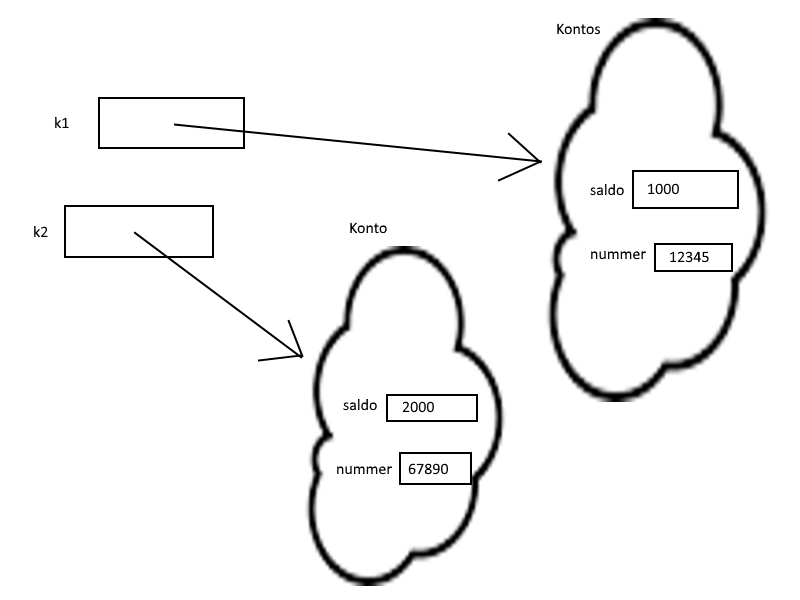
\includegraphics[scale=0.5]{../img/w04-solutions/uppgift-3a}
%
% \SubtaskSolved
% Tilldelningen på rad 8 \code{k1.nummer = 12345L} ger felmeddelande eftersom variablen är oföränderlig.
%
%
% \QUESTEND
%
%
%
%
% %%<AUTOEXTRACTED by mergesolu>%%      %Uppgift 3
%
%
%
%
% \WHAT{Klass med attribut som parametrar.}
%
% \QUESTBEGIN
%
% \Task  \what~  Om man vill ge attributen initialvärden när objektet skapas med \code{new}, kan man placera attributen i en parameterlista till klassen. Koden som körs när objektet skapas och attributen tilldelas sina initialvärden, kallas \textbf{konstruktor} \Eng{constructor}.
%
% \begin{REPL}
% scala> class Konto(var saldo: Int, val nummer: Long)
% scala> val k = new Konto(0, 12345L)
% scala> println("Konto: " + k.nummer + " Saldo:" + k.saldo)
% scala> println(k)
% scala> k.toString
% \end{REPL}
%
% \Subtask Den två sista raderna ovan skriver ut den identifierare som JVM använder för att hålla reda på objektet i sina interna datastrukturer. Vad skrivs ut?
%
% \Subtask Skapa ännu en instans av klassen Konto  med samma saldo och nummer som \code{k} ovan och spara den i \code{val k2} och undersök dess objektidentifierare. Får objekten \code{k} och \code{k2} olika objektidentifierare?
%
% \Subtask Sätt in olika belopp på respektive konto.
%
% \Subtask Vad händer om du försöker ändra attributet \code{nummer}?
%
% \Subtask\Pen Ibland räcker det fint med en tupel, men ofta vill man ha en klass istället. Beskriv några fördelar med en Konto-klassen ovan jämfört med en tupel av typen \code{(Int, Long)}.
%
% \begin{REPLnonum}
% scala> var k3 = (0, 12345L)
% scala> k3 = (k3._1 + 100, k3._2)
% \end{REPLnonum}
%
% \SOLUTION
%
%
% \TaskSolved \what
%
%
% \SubtaskSolved   \code{String = Konto@cd576}, där \code{Konto@cd576} är ett unikt namn som identifierar instansen.
%
% \SubtaskSolved   Ja.
%
% \SubtaskSolved
% \begin{REPLnonum}
% scala> k.saldo = 42
% scala> k2.saldo = 67
% \end{REPLnonum}
%
% \SubtaskSolved   Eftersom variablen är oföränderlig ges ett felmeddelande.
%
% \SubtaskSolved   En fördel med klass är att man kan specificera att variablen ska kunna vara föränderlig. En till är att man kan inkludera metoder i klassen som man vill kunna använda på värdena.
%
%
% \QUESTEND
%
%
%
%
% %%<AUTOEXTRACTED by mergesolu>%%      %Uppgift 4
%
%
%
%
% \WHAT{Publikt eller privat attribut?}
%
% \QUESTBEGIN
%
% \Task  \what~  Man kan förhindra att ett attribut syns utanför klassen med hjälp av nyckelordet \code{private}.
%
% \begin{REPL}
% scala> class Konto1(val nummer: Long){ var saldo = 0 }
% scala> val k1 = new Konto1(12345678901L)
% scala> k1.nummer
% scala> k1.saldo += 1000
% scala> class Konto2(val nummer: Long){ private var saldo = 0 }
% scala> val k2 = new Konto2(12345678901L)
% scala> k2.nummer
% scala> k2.saldo += 1000
% \end{REPL}
%
% \Subtask Vad händer ovan?
%
% \Subtask Gör en ny version av klassen \code{Konto} enligt nedan:
%
% \begin{Code}
% class Konto(val nummer: Long){
%   private var saldo = 0
%   def in(belopp: Int): Unit = {saldo += belopp}
%   def ut(belopp: Int): Unit = {saldo -= belopp}
%   def show: Unit =
%     println("Konto Nr: " + nummer + " saldo: " + saldo)
% }
%
% object Main {
%   def main(args: Array[String]): Unit = {
%     val k = new Konto(1234L)
%     k.show
%     k.in(1000)
%     println("Uttag: " + k.ut(500))
%     println("Uttag: " + k.ut(1000))
%     k.show
%   }
% }
% \end{Code}
%
% \Subtask Spara koden i en fil, kompilera med \code{scalac} och kör. Testa även vad som händer om du försöker komma åt attributet \code{saldo} i main-metoden med t.ex. \code{println(k.saldo)} eller \code{k.saldo += 1000}.
%
% \Subtask Vi ska nu förhindra överuttag. Ändra i metoden \code{ut} så att den får signaturen \code{ut(belopp: Int): (Int, Int) = ???} och implementera \code{ut} så att den returnerar både beloppet man verkligen kan ta ut och kvarvarande saldo. Om man försöker ta ut mer än det finns på kontot så ska saldot bli 0 och man får bara ut det som finns kvar. Spara, kompilera, kör.
%
% \Subtask Förbättra metoderna \code{in} och \code{ut} så att man inte kan sätta in eller ta ut negativa belopp.
%
% \Subtask Vad är fördelen med att göra föränderliga attribut privata och bara påverka deras värden indirekt via metoder?
%
% \SOLUTION
%
%
% \TaskSolved \what
%
%
% \SubtaskSolved
% Det går bra att ändra på variablen saldo i instansen av Konto1 men inte av Konto2 där man får ett error på raden ''k2.saldo += 1000''
%
% \SubtaskSolved  -
%
% \SubtaskSolved
% ''println(k.saldo)'' och ''k.saldo += 1000'' ger båda error, pga privat attribut.
%
% \SubtaskSolved
% \begin{Code}
% def ut(belopp: Int): (Int, Int) = {
% 	if(saldo >= belopp) {
% 		saldo -= belopp
% 		(belopp, saldo)
% 	} else {
% 		val temp = saldo
% 		saldo = 0
% 		(temp, 0)
% 	}
% }
% \end{Code}
%
% \SubtaskSolved
% Lägg till en if-sats i båda funktionerna som omsluter den gamla koden.
% \begin{Code}
% def ut(belopp: Int): (Int, Int) = {
%   if(belopp >= 0) {
%     if(saldo >= belopp) {
%       saldo -= belopp
%       (belopp, saldo)
%     } else {
%       val temp = saldo
%       saldo = 0
%       (temp, 0)
%     }
%   }
% }
%
% def in(belopp: Int): Unit = {
%   if(belopp >= 0) {
%     saldo += belopp
%   }
% }
% \end{Code}
%
% \SubtaskSolved
% Genom att göra attributet privat och gör egna metoder kan man se till att attriuten endast ändras på säkra sätt. Så inte fel uppstår.
%
%
% \QUESTEND
%
%
%
%
% %%<AUTOEXTRACTED by mergesolu>%%      %Uppgift 5
%
%
%
%
% \WHAT{Vilken typ har ett objekt?}
%
% \QUESTBEGIN
%
% \Task  \what~  Objektets typ bestäms av klassen. Vid tilldelning måste typerna passa ihop.
%
% \Subtask Vilka rader nedan ger felmeddelande? Hur lyder felmeddelandet?
% \begin{REPL}
% scala> class Punkt(val x: Double, val y: Double)
% scala> val pt: Punkt = new Punkt(10.0, 10.0)
% scala> val i: Int = pt.x
% scala> val (x: Double, y: Double) = (pt.x, pt.y)
% scala> val p: Double = new Punkt(5.0, 5.0)
% scala> val p = new Punkt(5.0, 5.0): Double
% scala> val p = new Punkt(5.0, 5.0): Punkt
% scala> pt: Punkt
% \end{REPL}
%
%
% \Subtask Man kan undersöka om ett objekt är av en viss typ med metoden \\ \code{isInstanceOf[Typnamn]}. Vad ger nedan anrop av metoden \code{isInstanceOf} för värde?
% \begin{REPL}
% scala> class Punkt(val x: Double, val y: Double)
% scala> val pt: Punkt = new Punkt(1.0, 2.0)
% scala> pt.isInstanceOf[Punkt]
% scala> pt.isInstanceOf[Double]
% scala> pt.x.isInstanceOf[Punkt]
% scala> pt.x.isInstanceOf[Double]
% scala> pt.x.isInstanceOf[Int]
% \end{REPL}
%
% \SOLUTION
%
%
% \TaskSolved \what
%
%
% \SubtaskSolved
% ''val i: Int = pt.x'' error: type mismatch;
% Eftersom typen Int ej är kompatibel med ett värde av typen Double.
%
% ''val p: Double = new Punkt(5.0, 5.0)'' error: type mismatch;
% Eftersom typen Double ej är kompatibel med ett värde av typen Punkt.
%
% ''val p = new Punkt(5.0, 5.0): Double'' error: type mismatch;
% Eftersom typen Double ej är kompatibel med ett värde av typen Punkt.
%
% \SubtaskSolved
% Rad 3 till 7 i respektive ordning: true, false, false, true och false.
%
%
% \QUESTEND
%
%
%
%
% %%<AUTOEXTRACTED by mergesolu>%%      %Uppgift 6
%
%
%
%
% \WHAT{Topptypen \code{Any}.}
%
% \QUESTBEGIN
%
% \Task  \what~ Alla klasser är också av typen \code{Any}. Alla klasser får därmed med sig några gemensamma metoder som finns i den fördefinierade klassen \code{Any}, däribland metoderna  \code{isInstanceOf} och \code{toString}.  Vad blir resultatet av respektive rad nedan? Vilken rad ger ett felmeddelande?
%
%
% \begin{REPL}
% scala> class Punkt(val x: Double, val y: Double)
% scala> val pt: Punkt = new Punkt(1.0, 2.0)
% scala> pt.isInstanceOf[Punkt]
% scala> pt.isInstanceOf[Any]
% scala> pt.x.toString
% scala> println(pt.x)
% scala> val a: Any = pt
% scala> println(a.x)
% scala> a.toString
% scala> pt.y.toString
% scala> a.y.toString
% \end{REPL}
%
% \SOLUTION
%
%
% \TaskSolved \what
%
% \begin{enumerate}
% \item Definierar klassen Punkt.
% \item En variabel pt: Punkt skapas.
% \item true
% \item true
% \item String = 1.0
% \item skriver ut: 1.0
% \item En variabel med namnet a skapas med typen Any.
% \item error: value x is not a member of Any
% \item a ges nu typen String
% \item String = 2.0
% \item error: value y is not a member of Any
% \end{enumerate}
%
%
% \QUESTEND
%
%
%
%
% %%<AUTOEXTRACTED by mergesolu>%%      %Uppgift 7
%
%
%
%
% \WHAT{Byta ut metoden \code{toString}}.
%
% \QUESTBEGIN
%
% \Task  \what~ I klassen \code{Any} finns metoden \code{toString} som skapar en strängrepresentation av objektet. Du kan byta ut metoden \code{toString} i klassen \code{Any} mot din egen implementation. Man använder nyckelordet \code{override} när man vill byta ut en metodimplementation.
%
% \begin{REPL}
% scala> class Punkt(val x: Double, val y: Double) {
%          override def toString: String = "[x=" + x + ",y=" + y + "]"
%        }
% scala> val pt = new Punkt(1.0, 42.0)
% scala> pt.toString
% scala> println(pt)
% \end{REPL}
%
% \Subtask Vad händer egentligen på sista raden ovan?
%
% \Subtask Omdefiniera toString så att den ger en sträng på formen \code{Punkt(1.0, 42.0)}.
%
% \Subtask Vad händer om du utelämnar nyckelordet \code{override} vid omdefiniering?
%
% \SOLUTION
%
%
% \TaskSolved \what
%
%
% \SubtaskSolved
% ''println(pt)'' kallar på pt.toString, och eftersom metoden är överskriven kallas den nya version.
%
% \SubtaskSolved   \code{override def toString: String = ''Punkt('' + x + '', '' + y + '').''}
%
% \SubtaskSolved
% error: overriding method toString in class Object of type ()String;
%
%
% \QUESTEND
%
%
%
%
% %%<AUTOEXTRACTED by mergesolu>%%      %Uppgift 8
%
%
%
%
% \WHAT{Objektfabrik med \code{apply}-metod.}
%
% \QUESTBEGIN
%
% \Task  \what~  Man kan ordna så att man slipper skriva \code{new} med ett s.k. \emph{fabriksobjekt} \Eng{factory object}.
% \begin{Code}
% class Pt(val x: Double, y: Double) {
%   override def toString: String = "Pt(x=" + x + ",y=" + y + ")"
% }
% object Pt {
%   def apply(x: Double, y: Double): Pt = new Pt(x, y)
% }
% \end{Code}
%
% \Subtask Skriv satser som använder metoden \code{apply} i fabriksobjektet \code{object Pt} för att skapa flera olika punkter.
%
% \Subtask Ge applymetoden default-argument 0.0 för både x och y så att \code{Pt()} skapar en punkt i origo.
%
% \Subtask Skapa en klass \code{Rational} som representerar rationellt tal som en kvot mellan två heltal. Ge klassen två oföränderliga, publika klassparameterattribut med namnen \code{nom} för täljaren och \code{denom} för nämnaren.
%
% \Subtask Skapa ett fabriksobjekt med en \code{apply}-metod som tar två heltalsparametrar och skapar en instans av klassen \code{Rational}.
%
% \Subtask Skapa olika instanser av din klass \code{Rational} ovan med hjälp av fabriksobjektet.
%
%
% \SOLUTION
%
%
% \TaskSolved \what
%
%
% \SubtaskSolved
% \begin{REPL}
% scala> val pt = Pt(1.0, 2.0)
% pt: Pt = Pt(x=1.0,y=2.0)
%
% scala> Pt(4.0, 2.0)
% res0: Pt = Pt(x=4.0,y=2.0)
%
% scala> Pt(6.0, 3.0)
% res1: Pt = Pt(x=6.0,y=3.0)
%
% scala> Pt(666.0, 1337.0)
% res2: Pt = Pt(x=666.0,y=1337.0)
% \end{REPL}
%
% \SubtaskSolved  \code{def apply(): Pt = new Pt(0, 0)}
%
% \SubtaskSolved  \code{class Rational(val nom: Int, val denom: Int)}
%
% \SubtaskSolved
% \begin{REPLnonum}
% object Rational {
% def apply(nom: Int, denom: Int): Rational = new Rational(nom, denom)
% }
% \end{REPLnonum}
%
% \SubtaskSolved
% \begin{REPL}
% scala> Rational(2, 5)
% scala> Rational(2, 7)
% scala> Rational(7, 4)
% scala> Rational(666, 1337)
% \end{REPL}
%
%
% \QUESTEND
%
%
%
%
% %%<AUTOEXTRACTED by mergesolu>%%      %Uppgift 9
%
%
%
%
% \WHAT{Skapa en case-klass.}
%
% \QUESTBEGIN
%
% \Task  \what~  Med en case-klass får man \code{toString} och fabriksobjekt på köpet. Man behöver inte skriva \code{val} framför klassparametrar i case-klasser; klassparametrar blir publika, oföränderliga attribut automatiskt när man deklarerar en case-klass.
%
% \begin{REPL}
% scala> case class Pt(x: Double, y: Double)
% scala> val p = Pt(1.0, 42.0)
% scala> p.toString
% scala> println(p)
% scala> println(Pt(5,6))
% \end{REPL}
%
% \Subtask Implementera din klass \code{Rational} från föregående uppgift, men nu som en case-klass.
%
% \SOLUTION
%
%
% \TaskSolved \what
%
% \SubtaskSolved  \code{case class Rational(nom: Int, denom: Int)}
%
%
% \QUESTEND
%
%
%
%
% %%<AUTOEXTRACTED by mergesolu>%%      %Uppgift 10
%
%
%
%
% \WHAT{Metoder på datastrukturer.}
%
% \QUESTBEGIN
%
% \Task \label{task:point} \what~   En datastruktur blir mer användbar om det finns metoder som kan användas på datastrukturen. Metoder i Scala kan även ha (vissa) specialtecken som namn, t.ex. \code{+} enligt nedan.
% \begin{REPL}
% scala> case class Point(x: Double, y: Double) {
%          def distToOrigin: Double = math.hypot(x, y)
%          def add(p: Point): Point = Point(x + p.x, y + p.y)
%          def +(p: Point): Point = add(p)
%        }
% \end{REPL}
%
% \Subtask Använd metoden \code{distToOrigin} för att ta reda på vad punkten med koordinaterna (3, 4) har för avstånd till origo?
%
% \Subtask Skriv satser som skapar två punkter (3,4) och (5, 6) och låt variablerna p1 och p2 referera till respektive punkt. Låt variabeln p3 bli summan av p1 och p2 med hjälp av metoden \code{add}. Vad får uttrycken \code{p3.x} resp. \code{p3.y} för värden?
%
%
%
% \SOLUTION
%
%
% \TaskSolved \what
%
%
% \SubtaskSolved
% \begin{REPLnonum}
% scala> Point(3, 4).distToOrigin
% res0: Double = 5.0
% \end{REPLnonum}
%
% \SubtaskSolved
% p3.x = 8
% p3.y = 10
%
%
% \QUESTEND
%
%
%
%
% %%<AUTOEXTRACTED by mergesolu>%%      %Uppgift 11
%
%
%
%
% \WHAT{Operatornotation.}
%
% \QUESTBEGIN
%
% \Task  \what~  Vid punktnotation på formen: \\ \code{objekt.metod(argument)} \\ kan man skippa punkten och parenteserna och skriva:\\ \code{objekt metod argument}  \\
% Detta förenklade skrivsätt kallas \textbf{operatornotation}.
%
% \Subtask Använd klassen \code{Point} från uppgift \ref{task:point} och prova nedan satser. Vilka rader använder operatortnotation och vilka rader använder punktnotation? Vilka rader ger felmeddelande?
% \begin{REPL}
% scala> val p1 = Point(3,4)
% scala> val p2 = Point(3,4)
% scala> p1.add(p2)
% scala> p1 add p2
% scala> p1.+(p2)
% scala> p1 + p2
% scala> 42 + 1
% scala> 42.+(1)
% scala> 42.+ 1
% scala> 42 +(1)
% scala> 1.to(42)
% scala> 1 to 42
% scala> 1.to(42)
% \end{REPL}
%
% \Subtask Implementera metoderna \code{sub} och \code{-} i klassen \code{Point} och skriv uttryck som kombinerar add och sub, samt + och - i både punktnotation och operatornotation.
%
% \Subtask Operatornotation fungerar även med flera argument. Man använder då parenteser om listan med argumenten:
% \code{ objekt metod (arg1, arg2)}  \\
% Definiera en metod \\
% \code{def scale(a: Double, b: Double) = Point(x * a, y * b)} \\
% i klassen \code{Point} och skriv satser som använder metoden med punktnotation och operatornotation.
%
%
%
%
%
% \SOLUTION
%
%
% \TaskSolved \what
%
%
% \SubtaskSolved
% \\Operatornotation:	4, 6, 10, 12
% \\Punktnotation:		3, 5, 8, 9, 11, 13
% \\Felmeddelande:		9
%
% \SubtaskSolved
% \begin{Code}
% case class Point(x: Double, y: Double) {
%   def distToOrigin: Double = math.hypot(x, y)
%   def add(p: Point): Point = Point(x + p.x, y + p.y)
%   def +(p: Point): Point = add(p)
%   def sub(p: Point): Point = Point(x - p.x, y - p.y)
%   def -(p: Point): Point = sub(p)
% }
% \end{Code}
% \begin{REPL}
% scala> val p1: Point = Point(1, 9)
% scala> val p2: Point = Point(9, 6)
% scala> p1.sub(p2)
% scala> p1.-(p2)
% scala> p2 sub p1
% scala> p2 - p2
% scala> p1.add(p2.sub(p1))
% scala> p1 + (p2 - p1)
% \end{REPL}
%
% \SubtaskSolved
% \begin{Code}
% case class Point(x: Double, y: Double) {
%   def distToOrigin: Double = math.hypot(x, y)
%   def add(p: Point): Point = Point(x + p.x, y + p.y)
%   def +(p: Point): Point = add(p)
%   def sub(p: Point): Point = Point(x - p.x, y - p.y)
%   def -(p: Point): Point = sub(p)
%   def scale(a: Double, b: Double) = Point(x * a, y * b)
% }
% \end{Code}
% \begin{REPL}
% scala> val p: Point(13,  37)
% scala> p.scale(4, 2)
% scala> p scale (3, 7)
% \end{REPL}
%
%
% \QUESTEND
%
%
%
%
% %%<AUTOEXTRACTED by mergesolu>%%      %Uppgift 12
%
%
%
%
% \WHAT{Föränderlighet och oföränderlighet.}
%
% \QUESTBEGIN
%
% \Task  \what~  Oföränderliga och föränderliga objekt beter sig olika vid tilldelning.
%
% \Subtask\Pen Innan du kör nedan kod: Försök lista ut vad som kommer att skrivas ut. Rita minnessituationen efter varje tilldelning.
%
% \begin{Code}
% println("\n--- Example 1: mutable value assigmnent")
% var x1 = 42
% var y1 = x1
% x1 = x1 + 42
% println(x1)
% println(y1)
% \end{Code}
%
% \Subtask\Pen Innan du kör nedan kod: Försök lista ut vad som kommer att skrivas ut. Rita minnessituationen efter varje tilldelning.
%
% \begin{Code}
% println("\n--- Example 2: mutable object reference assignment")
% class MutableInt(private var i: Int) {
%   def +(a: Int): MutableInt = { i = i + a; this }
%   override def toString: String = i.toString
% }
% var x2 = new MutableInt(42)
% var y2 = x2
% x2 = x2 + 42
% println(x2)
% println(y2)
% \end{Code}
%
% \Subtask\Pen Innan du kör nedan kod: Försök lista ut vad som kommer att skrivas ut. Rita minnessituationen efter varje tilldelning.
%
% \begin{Code}
% println("\n--- Example 3: immutable object reference assignment")
% class ImmutableInt(val i: Int) {
%   def +(a: Int): ImmutableInt = new ImmutableInt(i + a)
%   override def toString: String = i.toString
% }
% var x3 = new ImmutableInt(42)
% var y3 = x3
% x3 = x3 + 42
% println(x3)
% println(y3)
% \end{Code}
%
% \Subtask\Pen Vad finns det för fördelar med oföränderliga datastrukturer?
%
%
% \SOLUTION
%
%
% \TaskSolved \what
%
%
% \SubtaskSolved   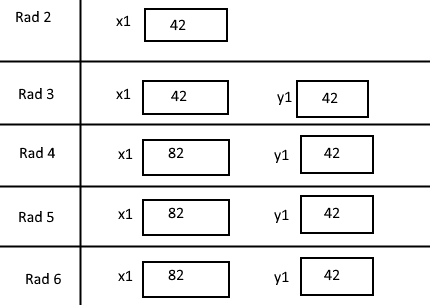
\includegraphics[scale=0.5]{../img/w04-solutions/uppgift-13a}
%
% \SubtaskSolved
% \begin{enumerate}
% \item 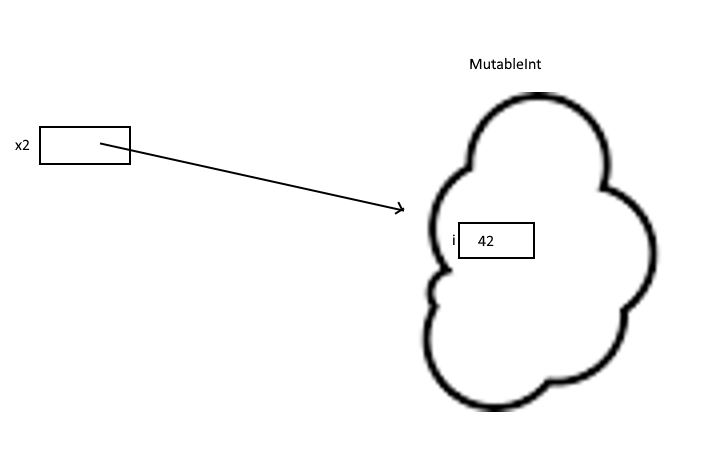
\includegraphics[scale=0.5]{../img/w04-solutions/uppgift-13b-1}
% \item 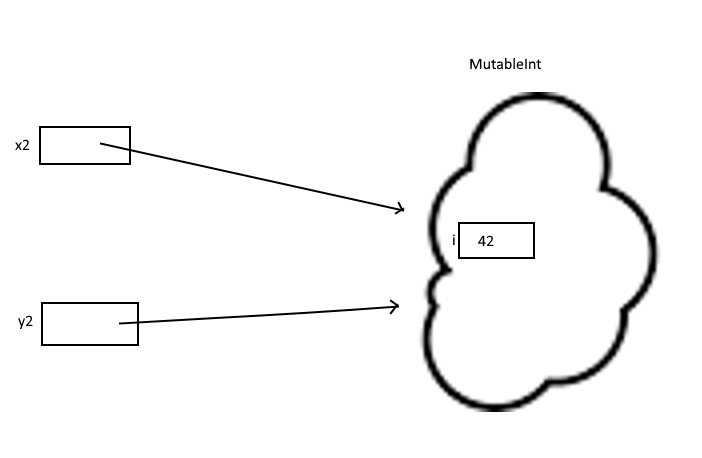
\includegraphics[scale=0.5]{../img/w04-solutions/uppgift-13b-2}
% \item 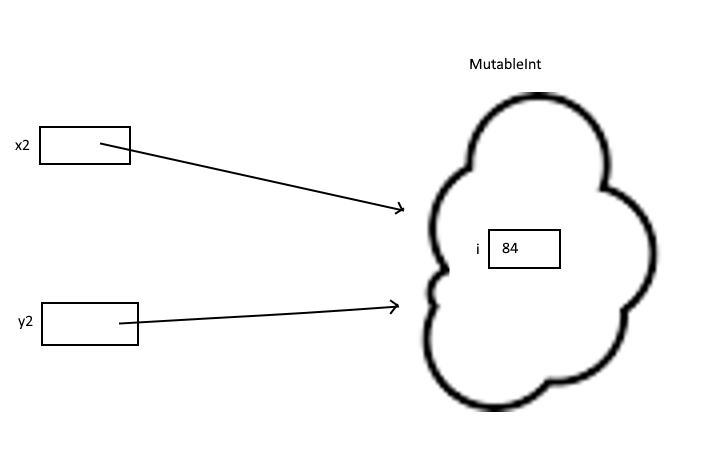
\includegraphics[scale=0.5]{../img/w04-solutions/uppgift-13b-3}
% \end{enumerate}
%
% \SubtaskSolved
% \begin{enumerate}
% \item 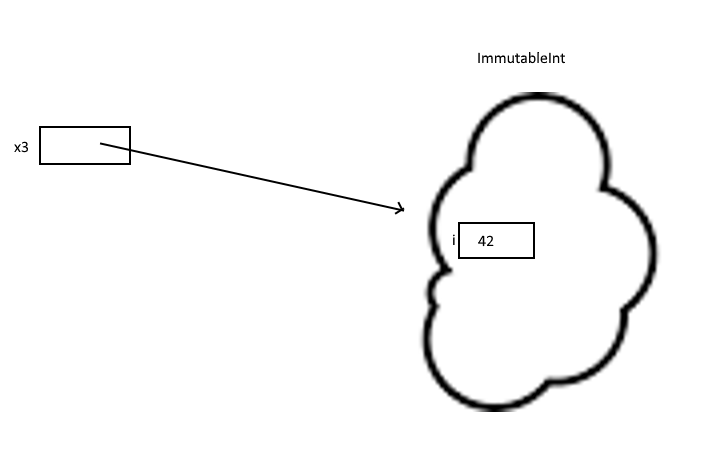
\includegraphics[scale=0.5]{../img/w04-solutions/uppgift-13c-1}
% \item 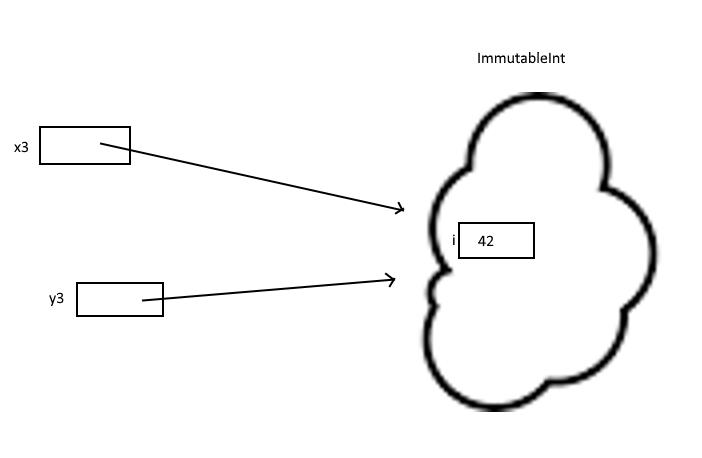
\includegraphics[scale=0.5]{../img/w04-solutions/uppgift-13c-2}
% \item 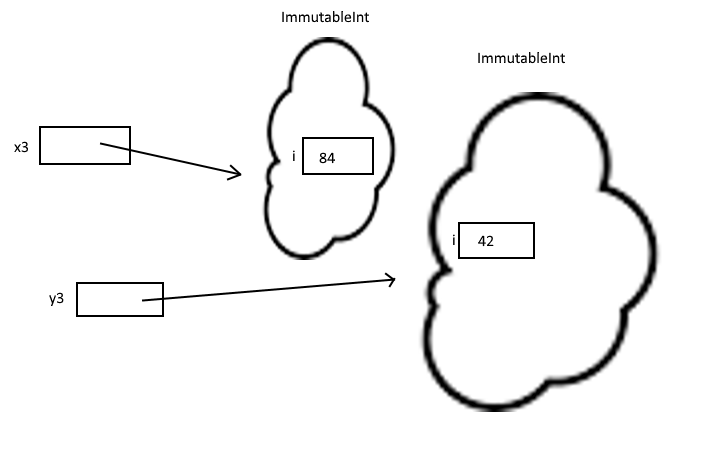
\includegraphics[scale=0.5]{../img/w04-solutions/uppgift-13c-3}
% \end{enumerate}
%
% \SubtaskSolved   En stor fördel är att vi till exempel kan skicka med en immutable som argument till en metod och vara säkra på att metoden inte ändrar på värdet.
%
%
% \QUESTEND
%
%
%
%
% %%<AUTOEXTRACTED by mergesolu>%%      %Uppgift 13
%
%
%
%
% \WHAT{Några användbara samlingar.}
%
% \QUESTBEGIN
%
% \Task  \what~  En \textbf{samling} \Eng{collection} är en datastruktur som samlar många objekt av samma typ. I \code{scala.collection} och \code{java.util} finns många olika samlingar med en uppsjö användbara metoder. De olika samlingarna i \code{scala.collection} är ordnade i en gemensam hierarki med många gemensamma metoder; därför har man nytta av det man lär sig om metoderna i en Scala-samling när man använder en annan samling. Vi har redan tidigare sett samlingen \code{Vector}:
%
% \begin{REPL}
% scala> val tärningskast = Vector.fill(10000)((math.random() * 6 + 1).toInt)
% scala> tä   // tryck TAB
% scala> tärningskast.  // tryck TAB
% \end{REPL}
%
% \Subtask Ungefär hur många metoder finns det som man kan göra på objekt av typen \code{Vector}? Det är svårt att lära sig alla dessa på en gång, så vi väljer ut några få i kommande uppgifter.
%
% \Subtask Jämför överlappet mellan metoderna i \code{Vector} och \code{List} och uppskatta hur stor andel av metoderna som är gemensamma:
% \begin{REPL}
% scala> val myntkast =
%          List.fill(10000)(if (math.random() < 0.5) "krona" else "klave")
% scala> my   // tryck TAB
% scala> myntkast.  // tryck TAB
% \end{REPL}
%
% \SOLUTION
%
%
% \TaskSolved \what
%
%
% \SubtaskSolved   Ungefär 150 metoder.
%
% \SubtaskSolved   Ungefär lika många.
%
%
% \QUESTEND
%
%
%
%
% %%<AUTOEXTRACTED by mergesolu>%%      %Uppgift 14
%
%
%
%
% \WHAT{Typparameter.}
%
% \QUESTBEGIN
%
% \Task  \what~  Vissa funktioner är generella för många typer och tar en så kallad \textbf{typparameter} inom hakparenteser. Ofta slipper man skriva typparametrar, då kompilatorn kan härleda typen utifrån argumenten. Om man anger typparametrar explicit så hjälper kompilatorn dig med att kolla att det verkligen är rätt typ i samlingen.
%
% \Subtask Vad händer nedan?
% \begin{REPL}
% scala> var xs = Vector.empty[Int]
% scala> xs = xs :+ "42"
% scala> xs = xs :+ 43 :+ 64 :+ 46
% scala> xs
% scala> xs :+= "42".toInt
% scala> var ys = Vector[Int]("ett", "två", "tre")
% scala> var ingenting = Vector.empty
% scala> ingenting = Vector(1,2,3)
% \end{REPL}
%
% \Subtask Samlingar är mer användbara om de är \emph{generiska}, vilket innebär att elementens typ avgörs av en typparameter och därför kan vara av vilken typ som helst. Man kan definiera egna funktioner som tar generiska samlingar som parametrar. Förklara vad som händer här:
% \begin{REPL}
% scala> val vego = Vector("gurka", "tomat", "apelsin", "banan")
% scala> val prim = Vector(2, 3, 5, 7, 11, 13)
% scala> def först[T](xs: Vector[T]): T = xs.head
% scala> def sist[T](xs: Vector[T]) = xs.last
% scala> def förstOchSist[T](xs: Vector[T]): (T, T) = (xs.head, xs.last)
% scala> först(vego)
% scala> sist(prim)
% scala> förstOchSist(vego)
% scala> förstOchSist(prim)
% scala> def wrap[T](pair: (T, T))(xs: Vector[T]) = pair._1 +: xs :+ pair._2
% scala> wrap("Odla", "och ät!")(vego)
% scala> wrap("Odla", "och ät!")(vego).mkString(" ")
% \end{REPL}
%
%
%
%
%
% \SOLUTION
%
%
% \TaskSolved \what
%
%
% \SubtaskSolved
% \\1. Instansierar en tom vektor med element av typen int och tilldelar värdet till en variabel xs.
% \\2. Error eftersom \code{xs :+ ''42''} ger en Vector[Any] när Vector[Int] krävs.
% \\3. xs tilldelas ett nytt värde av Vector(43, 64, 46)
% \\4. xs skrivs ut.
% \\5. Lägger till talet 42 i xs.
% \\6. Error: type mismatch
% \\7. Skapar en tom Vector i variablen ingenting
% \\8. error: type mismatch; found: Int(3), required: Nothing
%
% \SubtaskSolved
% Tre metoder skapas: den första för att få första elementet i en lista, och eftersom den definieras med specialtypen T går den att använda med alla vektorer oavsett typen av variabeln i vektorn. Den andra får fram sista elementet och den sista hämtar båda två.
%
% En till function definieras längre ner med  namnet ''wrap'', som tar en lista och lägger till ett element längst fram och ett längst bak.
%
%
% \QUESTEND
%
%
%
%
% %%<AUTOEXTRACTED by mergesolu>%%      %Uppgift 15
%
%
%
%
% \WHAT{Några viktiga samlingsmetoder.}
%
% \QUESTBEGIN
%
% \Task  \what~  Deklarera följande vektorer i REPL.
% \begin{REPL}
% scala> val xs = (1 to 10).toVector
% scala> val a = Vector("abra", "ka", "dabra")
% scala> val b = Vector( "sim", "sala", "bim", "sala", "bim")
% scala> val stor = Vector.fill(100000)(math.random())
% \end{REPL}
% Undersök i REPL vad som händer nedan. Alla dessa metoder fungerar på alla samlingar som är indexerbara sekvenser. Givet deklarationerna ovan: vad har uttrycken nedan för värde och typ? Förklara vad som händer hälp av denna  översikt: \href{http://docs.scala-lang.org/overviews/collections/seqs}{docs.scala-lang.org/overviews/collections/seqs}
%
% \Subtask \code{a(1) + xs(1)}
%
% \Subtask \code{a apply 0}
%
% \Subtask \code{a.isDefinedAt(3)}
%
% \Subtask \code{a.isDefinedAt(100)}
%
% \Subtask \code{stor.length}
%
% \Subtask \code{stor.size}
%
% \Subtask \code{stor.min}
%
% \Subtask \code{stor.max}
%
% \Subtask \code{a indexOf "ka"}
%
% \Subtask \code{b.lastIndexOf("sala")}
%
% \Subtask \code{"först" +: b   //minnesregel: colon on the collection side}
%
% \Subtask \code{a :+ "sist"    //minnesregel: colon on the collection side}
%
% \Subtask \code{xs.updated(2,42)}
%
% \Subtask \code{a.padTo(10, "!")}
%
% \Subtask \code{b.sorted}
%
% \Subtask \code{b.reverse}
%
% \Subtask \code{a.startsWith(Vector("abra", "ka"))}
%
% \Subtask \code{"hejsan".endsWith("san")}
%
% \Subtask \code{b.distinct}
%
%
%
% \SOLUTION
%
%
% \TaskSolved \what
%
%
% \SubtaskSolved   String = ''ka2''
%
% \SubtaskSolved   String = ''abra''
%
% \SubtaskSolved   false
%
% \SubtaskSolved   false
%
% \SubtaskSolved   100000
%
% \SubtaskSolved   100000
%
% \SubtaskSolved   minsta talet i listan
%
% \SubtaskSolved   största talet i listan
%
% \SubtaskSolved   1
%
% \SubtaskSolved   3
%
% \SubtaskSolved   Vektor b fast med ''först'' som första element
%
% \SubtaskSolved   Vektor a fast med ''sist'' som sista element.
%
% \SubtaskSolved   plats 3 i vektorn xs får värdet 42
%
% \SubtaskSolved   En ny vektor fylld med ''!'' från och med plats 4 till 10. Men de andra värdena samma som i a.
%
% \SubtaskSolved   b sorterad i bokstavsordning
%
% \SubtaskSolved   b baklänges
%
% \SubtaskSolved   true
%
% \SubtaskSolved   true
%
% \SubtaskSolved   en vektor med alla unika element i b.
%
%
% \QUESTEND
%
%
%
%
% %%<AUTOEXTRACTED by mergesolu>%%      %Uppgift 16
%
%
%
%
% \WHAT{Några generella samlingsmetoder.}
%
% \QUESTBEGIN
%
% \Task  \what~  Det finns metoder som går att köra på \emph{alla} samlingar även om de inte är indexerbara. Givet deklarationerna i föregående uppgift: vad har uttrycken nedan för värde och typ? Förklara vad som händer med hjälp av dessa översikter: \\ \href{http://docs.scala-lang.org/overviews/collections/trait-traversable}{docs.scala-lang.org/overviews/collections/trait-traversable} \\ \href{http://docs.scala-lang.org/overviews/collections/trait-iterable}{docs.scala-lang.org/overviews/collections/trait-iterable}
%
% \Subtask \code{a ++ b}
%
% \Subtask \code{a ++ stor}
%
% \Subtask \code{val ys = xs.map(_ * 5)}
%
% \Subtask \code{b.toSet     // En mängd har inga dubletter}
%
% \Subtask \code{a.head + b.last}
%
% \Subtask \code{a.tail}
%
% \Subtask \code{a.head +: a.tail == a}
%
% \Subtask \code{Vector(a.head) ++ Vector(b.last)}
%
% \Subtask \code{a.take(1) ++ b.takeRight(1)}
%
% \Subtask \code{a.drop(2) ++ b.drop(1).dropRight(2)}
%
% \Subtask \code{a.drop(100)}
%
% \Subtask \code{val e = Vector.empty[String]; e.take(100)}
%
% \Subtask \code{Vector(e.isEmpty, e.nonEmpty)}
%
% \Subtask \code{a.contains("ka")}
%
% \Subtask \code{"ka" contains "a"}
%
% \Subtask \code{a.filter(s => s.contains("k")) }
%
% \Subtask \code{a.filter(_.contains("k")) }
%
% \Subtask \code{a.map(_.toUpperCase).filterNot(_.contains("K")) }
%
% \Subtask \code{xs.filter(x => x % 2 == 0)}
%
% \Subtask \code{xs.filter(_ % 2 == 0)}
%
%
% \SOLUTION
%
%
% \TaskSolved \what
%
%
% \SubtaskSolved
% Metoden ger tillbaka en ny Vector[String] som nu består av alla element i a plus alla element i b. I samma ordning med elementen i a först.
%
% \SubtaskSolved
% Samma som i uppgift a fast vektorn som returnas är av typen Vector[Any]. Det är eftersom Any är den närmsta typen som String och Double delar. Elementen från vektor a är fortfarande först och uppföljt av elementen i stor.
%
% \SubtaskSolved
% Variablen ys får värdet av en Vector[Int] som innehåller alla talen från xs fast multiplicerade med 5. Alltså ys = 5, 10, 15..., osv.
%
% \SubtaskSolved
% Functionen tar alla värden från en Vektor och sätter in i ett Set (mängd). Eftersom en mängd ej har dubletter så försvinner ett ''sala'' och ett ''bim'', Vector[String] som returneras blir därför (''sim'', ''sala'', ''bim'').
%
% \SubtaskSolved
% Metoden head ger första elementet i en samling, och last sista. Därför blir kombinationen av a.head och b.last en ny Vector[String] som består av a:s första element, och b:s första element.
%
% \SubtaskSolved
% Ger en Vector[String] som innehåller alla element efter det första. Alltså i detta fallet ''ka'' och ''dabra''.
%
% \SubtaskSolved
% True, eftersom head ger första elementet och tail ger resten, sedan sätter metoden +: ihop dem till en vektor med samma värden som a.
%
% \SubtaskSolved
% Eftersom ++ sätter ihop alla värden från två vektorer måste vi först omvandla från en sträng till vektor. Resultatet blir en ny vektor av samma typ som innan med a:s första element och b:S sista.
%
% \SubtaskSolved
% Samma resultat som i h, metoden take börjar från vänster och tar så många element som man skickar med som parameter och gör till en ny lista. Med 1 som parameter motsvarar det att göra Vector(a.head). Metoden takeRight gör samma sak fast från höger.
%
% \SubtaskSolved
% Metoden drop är motsvarigheten till take fast exkluderar de specifierade elementen istället för att inkludera dem i vektorn.
%
% \SubtaskSolved
% Eftersom a endast innehåller 3 element returnerar drop(100) en tom vektor.
%
% \SubtaskSolved
% Returnerar en tom vektor med element typen String
%
% \SubtaskSolved
% returnerar Vector(true, false)
%
% \SubtaskSolved
% True, metoden contains kollar om en samling innehåller ett specifikt element.
%
% \SubtaskSolved
% True. Eftersom en sträng även kan ses som Vector[Char].
%
% \SubtaskSolved
% Filtrerar vektorn a till att endast innehålla strängar som innehåller k.
%
% \SubtaskSolved
% Exakt samma som i p
%
% \SubtaskSolved
% map(\_.toUpperCase) omvandlar alla strängar i a till stora bokstäver
% filterNot(\_.contains(''K'')) tar resultatet vi precis fick och tar bort alla strängar som innehåller stora K.
%
% \SubtaskSolved
% filtrerar så att endast jämna tal finns kvar.
%
% \SubtaskSolved
% Exakt samma som i s
%
%
%
%
% \QUESTEND
%
%
%
%
% %%<AUTOEXTRACTED by mergesolu>%%      %Uppgift 17
%
%
%
%
% \WHAT{NEEDS A TOPIC DESCRIPTION}
%
% \QUESTBEGIN
%
% \Task  \what~ De olika samlingarna i \code{scala.collection} används flitigt i andra paket, exempelvis \code{scala.util} och \code{scala.io}.
%
% \Subtask Vad händer här? (Metoden \code{shuffle} skapar en ny samling med elementen i slumpvis ordning.)
% \begin{REPL}
% val xs = Vector(1,2,3)
% def blandat = scala.util.Random.shuffle(xs)
% def test = if (xs == blandat) "lika" else "olika"
% (for(i <- 1 to 100) yield test).count(_ == "lika")
% \end{REPL}
%
%
% \Subtask Skapa en textfil med namnet \code{fil.txt} som innehåller lite text och läs in den med: \\\code{scala.io.Source.fromFile("fil.txt", "UTF-8").getLines.toVector}
% \begin{REPL}
% > cat > fil.txt
% hejsan
% svejsan
% > scala
% scala> val xs = scala.io.Source.fromFile("fil.txt", "UTF-8").getLines.toVector
% scala> xs.foreach(println)
% \end{REPL}
%
%
% \Subtask Vad händer här? (Metoden \code{trim} på värden av typen \code{String} ger en ny sträng med blanktecken i början och slutet borttagna.)
% \begin{REPL}
% scala> val pgk =
%   scala.io.Source.fromURL("http://cs.lth.se/pgk/","UTF-8").getLines.toVector
% scala> pgk.foreach(println)
% scala> pgk.map(_.trim).
%          filterNot(_.startsWith("<")).
%          filterNot(_.isEmpty).
%          foreach(println)
% \end{REPL}
%
%
%
% \SOLUTION
%
%
% \TaskSolved \what
%
%
% \SubtaskSolved
% Vi instansierar en vektor xs med talen 1, 2 och 3.
% sedan definierar vi en metod blandat som ger oss en randomiserad version av xs.
% sedan definierar vi en till metod som testar om xs är lika med resultatet från blandat. Om det är så returnerar den strängen ''lika'' annars ''olika''.
% Sist kör vi en for-loop där vi 100 gånger kör testet, samtidigt räknas hur många gånger ''lika'' returneras.
%
% Vårt resultat är en siffra på hur många gånger xs var samma som en blandad version av sig själv, eftersom det finns 6 permutationer med 3 variabler så borde det vara ungefär 1/6 chans.
%
% \SubtaskSolved  -
%
% \SubtaskSolved
% \\ \code{map(\_.trim)} tar bort alla onödiga mellanrum i början och slutet på varje rad
% \\ \code{filterNot(\_.startsWith(''<''))} filtrerar bort alla rader som börjar med strängen ''<''
% \\ \code{filterNot(\_.isEmpty)} filtrerar bort alla tomma rader.
% \\ \code{foreach(println)} skriver ut alla rader.
%
%
% \QUESTEND
%
%
%
%
% %%<AUTOEXTRACTED by mergesolu>%%      %Uppgift 18
%
%
%
%
% \WHAT{Jämföra List och Vector.}
%
% \QUESTBEGIN
%
% \Task  \what~  En indexerbar sekvens av värden kallas vektor eller lista. I Scala finns flera klasser som kan kan indexeras, däribland klasserna \code{Vector} och \code{List}.
%
% \Subtask \emph{Likheter mellan \code{Vector} och \code{List}.} Kör nedan rader i REPL. Prova indexera i båda och studera hur stor andel av metoderna som är gemensamma.
% \begin{REPL}
% scala> val sv = Vector("en", "två", "tre", "fyra")
% scala> val en = List("one", "two", "three", "four")
% scala> sv(0) + sv(3)
% scala> en(0) + en(3)
% scala> sv. //tryck TAB
% scala> en. //tryck TAB
% \end{REPL}
%
% \Subtask \emph{Skillnader mellan \code{Vector} och \code{List}.} Klassen \code{Vector} i Scala har ''under huven'' en avancerad datastruktur i form av ett s.k. självbalanserande träd, vilket gör att \code{Vector} är snabbare än \code{List} på nästan allt, \emph{utom} att bearbeta elementen i \emph{början} av sekvensen; vill man lägga till och ta bort i början av en \code{List} så kan det ibland gå ungefär dubbelt så fort jämfört med \code{Vector}, medan alla andra operationer är lika snabba eller snabbare med \code{Vector}. Det finns ett fåtal speciella metoder, som bara finns i \code{List}, för att skapa en lista och lägga till i början av en lista. Vad händer nedan?
%
% \begin{REPL}
% scala> var xs = "one" :: "two" :: "three" :: "four" :: Nil
% scala> xs = "zero" :: xs
% scala> val ys = xs.reverse ::: xs
% \end{REPL}
%
%
% \SOLUTION
%
%
% \TaskSolved \what
%
%
% \SubtaskSolved
% I princip alla metoder delas, en lista har några fler t. ex. ''::'', '':::'', ''mapConserve'' osv.
%
% \SubtaskSolved
% Först skapas en lista med 4 sträng värden och instansierar variablen xs med det värdet.
% sedan skapar vi en ny lista, som består av ''zero'' + den gamla listan och ger värdet till xs.
% Sist instansierar vi en ny variabel ys, som får värdet av xs omvänd plus xs.
%
%
% \QUESTEND
%
%
%
%
% %%<AUTOEXTRACTED by mergesolu>%%      %Uppgift 19
%
%
%
%
% \WHAT{Mängd.}
%
% \QUESTBEGIN
%
% \Task  \what~  En mängd är en samling som garanterar att det inte finns några dubbletter. Det går dessutom väldigt snabbt, även i stora mängder, att kolla om ett element finns eller inte i mängden. Elementen i samlingen \code{Set} hamnar ibland, av effektivitetsskäl, i en förvånande ordning.
% \begin{REPL}
% scala> val s = Set("Malmö", "Stockholm", "Göteborg", "Köpenhamn", "Oslo")
% s: scala.collection.immutable.Set[String] =
%      Set(Oslo, Malmö, Köpenhamn, Stockholm, Göteborg)
%
% scala> val t = Set("Sverige", "Sverige", "Sverige", "Danmark", "Norge")
% t: scala.collection.immutable.Set[String] = Set(Sverige, Danmark, Norge)
% \end{REPL}
% Givet ovan deklarationer: vad blir värde och typ av nedan uttryck?
%
% \Subtask \code{s + "Malmö" == s}
%
% \Subtask \code{s ++ t}
%
% \Subtask \code{Set("Malmö", "Oslo").subsetOf(s)}
%
% \Subtask \code{s subsetOf Set("Malmö", "Oslo")}
%
% \Subtask \code{s contains "Lund"}
%
% \Subtask \code{s apply "Lund"}
%
% \Subtask \code{s("Malmö")}
%
% \Subtask \code{s - "Stockholm"}
%
% \Subtask \code{t - ("Norge", "Danmark", "Tyskland")}
%
% \Subtask \code{s -- t}
%
% \Subtask \code{s -- Set("Malmö", "Oslo")}
%
% \Subtask \code{Set(1,2,3) intersect Set(2,3,4)}
%
% \Subtask \code{Set(1,2,3) & Set(2,3,4)}
%
% \Subtask \code{Set(1,2,3) union Set(2,3,4)}
%
% \Subtask \code{Set(1,2,3) | Set(2,3,4)}
%
%
% \SOLUTION
%
%
% \TaskSolved \what
%
%
% \SubtaskSolved
% true, Boolean
%
% \SubtaskSolved
% En samling av alla värden i s och t, Set[String]
%
% \SubtaskSolved
% true, Boolean
%
% \SubtaskSolved
% false, Boolean
%
% \SubtaskSolved
% false, Boolean
%
% \SubtaskSolved
% false, Boolean
%
% \SubtaskSolved
% true, Boolean
%
% \SubtaskSolved
% Samlingen s utan elementet ''Stockholm'', Set[String]
%
% \SubtaskSolved
% Samlingen t utan elementen ''Norge'' och ''Danmark'', Set[String]
%
% \SubtaskSolved
% returnerar s, Set[String]
%
% \SubtaskSolved
% Samlingen s utan ''Malmö'' och ''Oslo'', Set[String]
%
% \SubtaskSolved
% Set(2, 3), Set[Int]
%
% \SubtaskSolved
% se deluppgift l
%
% \SubtaskSolved
% Set(1, 2, 3 ,4), Set[Int]
%
% \SubtaskSolved
% se deluppgift n
%
%
% \QUESTEND
%
%
%
%
% %%<AUTOEXTRACTED by mergesolu>%%      %Uppgift 20
%
%
%
%
% \WHAT{Slå upp värden från nycklar med \code{Map}.}
%
% \QUESTBEGIN
%
% \Task  \what~  Samlingen \code{Map} är mycket användbar. Med den kan man snabbt leta upp ett värde om man har en nyckel. Samlingen \code{Map} är en generalisering av en vektor, där man kan ''indexera'', inte bara med ett heltal, utan med vilken typ av värde som helst, t.ex. en sträng. Datastrukturen \code{Map} är en s.k. \emph{associativ array}\footnote{\href{https://en.wikipedia.org/wiki/Associative_array}{https://en.wikipedia.org/wiki/Associative\_array}}, implementerad som en s.k. \emph{hashtabell}\footnote{\href{https://en.wikipedia.org/wiki/Hash_table}{https://en.wikipedia.org/wiki/Hash\_table}}.
% \begin{REPL}
% scala> var huvudstad =
%   Map("Sverige" -> "Stockholm", "Norge" -> "Oslo", "Skåne" -> "Malmö")
% \end{REPL}
% Givet ovan variabel \code{huvudstad}, förklara vad som händer nedan?
%
% \Subtask \code{huvudstad apply "Skåne"}
%
% \Subtask \code{huvudstad("Sverige")}
%
% \Subtask \code{huvudstad.contains("Skåne")}
%
% \Subtask \code{huvudstad.contains("Malmö")}
%
% \Subtask \code{huvudstad += "Danmark" -> "Köpenhamn"}
%
% \Subtask \code{huvudstad.foreach(println)}
%
% \Subtask \code{huvudstad getOrElse ("Norge", "???") }
%
% \Subtask \code{huvudstad getOrElse ("Finland", "???") }
%
% \Subtask \code{huvudstad.keys.toVector.sorted}
%
% \Subtask \code{huvudstad.values.toVector.sorted}
%
% \Subtask \code{huvudstad - "Skåne"}
%
% \Subtask \code{huvudstad - "Jylland"}
%
% \Subtask \code{huvudstad = huvudstad.updated("Skåne","Lund") }
%
%
%
% \SOLUTION
%
%
% \TaskSolved \what
%
%
% \SubtaskSolved
% Returnerar strängen ''Malmö'' eftersom det värdet är indexerat på platsen ''Skåne''.
%
% \SubtaskSolved
% Returnerar strängen ''Stockholm'' eftersom det värdet är indexerat på platsen ''Sverige''.
%
% \SubtaskSolved
% true, eftersom huvudstad innehåller indexet ''Skåne''
%
% \SubtaskSolved
% false, eftersom huvudstad ej innehåller indexet ''Malmö''. Notera att det är index och inte värden vi
% kollar om det finns.
%
% \SubtaskSolved
% Lägger till indexet ''Danmark'' med värdet ''Köpenhamn'' i samlingen.
%
% \SubtaskSolved
% Skriver ut alla 2-tupler.
%
% \SubtaskSolved
% Returnerar ''Oslo'', Note: Om indexet ''Norge'' inte hade funnits hade ''???'' returnerats istället.
%
% \SubtaskSolved
% Returnerar ''???''
%
% \SubtaskSolved
% Returnerar en sorterar vektor med alla index.
%
% \SubtaskSolved
% Returnerar en sorterar vektor med alla värden.
%
% \SubtaskSolved
% Returnerar en ny mängd men med ''Skåne'' -> ''Malmö'' borttaget.
%
% \SubtaskSolved
% Returnerar huvudstad mängden eftersom det inte finns ett ''Jylland'' index att ta bort.
%
% \SubtaskSolved
% Uppdaterar indexet ''Skåne'' till att istället leda till värdet ''Lund''
%
%
% \QUESTEND
%
%
%
%
% %%<AUTOEXTRACTED by mergesolu>%%      %Uppgift 21
%
%
%
%
% \WHAT{Skapa Map från en samling.}
%
% \QUESTBEGIN
%
% \Task  \what~
%
% \Subtask Definiera denna vektor och undersök dess typ:
% \begin{Code}
% val pairs = Vector(
%   ("Björn", 46462229009L),
%   ("Maj", 46462221667L),
%   ("Gustav", 46462224906L))
% \end{Code}
%
% \Subtask Vad har variablen \code{telnr} nedan för typ: \\ \code{var telnr = pairs.toMap}
%
% \Subtask Använd \code{telnr} för att slå upp telefonnummer för Maj och Kim med hjälp av metoderna \code{apply} och \code{get}.
%
% \Subtask Använd metoden \code{getOrElse} vid upplagningar av \code{telnr} och ge \code{-1L} som telefonnummer i händelse av att ett nummer inte finns.
%
% \Subtask Lägg till \code{("Fröken Ur", 464690510L)} i \code{telnr}-mappen.
%
% \Subtask Skapa en \code{Vector[(String, String)]} enligt nedan, så att telefonnumret blir en sträng utan inledande landsnummer men med en nolla i riktnumret. Byt ut \code{???} mot lämpligt uttryck.
% \begin{REPL}
% scala> telnr.toVector.map(p => ???)
% res85: Vector[(String, String)] = Vector(("Björn", "0462229009"), ("Maj",
% "0462221667"), ("Gustav", "0462224906"), ("Fröken Ur", 04690510"))
%
% \end{REPL}
%
% \Subtask Använd vektorn i resultatet ovan för att skapa en ny \code{Map[String, String]} med nationella telefonnumer. Slå upp numret till Fröken Ur.
%
% \SOLUTION
%
%
% \TaskSolved \what
%
%
% \SubtaskSolved
% \begin{REPLnonum}
% pairs: scala.collection.immutable.Vector[(String, Long)] =
% 					Vector((Björn,444), (Maj,441), (Lucy,666))
% \end{REPLnonum}
%
% \SubtaskSolved
% Map[String, Long]
%
% \SubtaskSolved
% \begin{REPLnonum}
% scala> telnr(''Maj'')
% res0: Long = 441
%
% scala> telnr.get(''Maj'')
% res1: Option[Long] = Some(441)
%
% scala> telnr(''Kim'')
% java.util.NoSuchElementException: key not found: 'Kim
%   at scala.collection.MapLike$class.default(MapLike.scala:228)
%   at scala.collection.AbstractMap.default(Map.scala:59)
%   at scala.collection.MapLike$class.apply(MapLike.scala:141)
%   at scala.collection.AbstractMap.apply(Map.scala:59)
%   ... 32 elided
%
% scala> telnr.get(''Kim'')
% res2: Option[Long] = None
% \end{REPLnonum}
%
% \SubtaskSolved
% \begin{REPLnonum}
% scala> telnr.getOrElse(''Maj'', -1L)
% res0: Long = 441
%
% scala> telnr.getOrElse(''Kim'', -1L)
% res1: Long = -1
% \end{REPLnonum}
%
% \SubtaskSolved
% telnr += ''Fröken Ur'' -> 464690510L
%
% \SubtaskSolved
% telnr.toVector.map(p => p.\_1 -> (''0'' + p.\_2.toString.substring(2)))
%
% \SubtaskSolved
% Använd metoden toMap och apply.
%
%
%
%
% \QUESTEND
%
%
%
%
% %%<AUTOEXTRACTED by mergesolu>%%      %Uppgift 22
%
%
%
%
% \WHAT{Samlingsmetoden \code{maxBy}.}
%
% \QUESTBEGIN
%
% \Task  \what~  Med samlingsmetoden \code{maxBy} kan man själv definiera vad som ska maximeras. (Denna metod kommer du att behöva i veckans laboration.)
%
% \Subtask Förklara vad som händer nedan.
% \begin{REPL}
% scala> val xs = Vector((2,3), (1,5), (-1, 1), (7, 2))
% scala> xs.maxBy(x => x._1)
% scala> xs.maxBy(x => x._2)
% \end{REPL}
%
% \Subtask Om man bara använder en parameter i en anonym funktion, till exempel parametern \code{x} i lambdauttrycket \code{x => x + 1} \emph{en enda} gång, och kompilatorn kan gissa alla typer, kan man använda understreck som ''platshållare'' för att förkorta lambdauttrycket så här: \code{ _ + 1}
%
% Skriv uttrycken på raderna 2 och 3 i föregående deluppgift på ett kortare sätt med hjälp platshållarsyntax \Eng{place holder syntax}.
%
% \Subtask På motsvarande sätt kan man använda \code{minBy} för att välja vilken funktion som definierar minimum. Prova \code{minBy} på motsvarande sätt som i föregående deluppgifter.
%
% \SOLUTION
%
%
% \TaskSolved \what
%
%
% \SubtaskSolved   Metoden maxBy hämtar det element som är ''störst'', på rad två gör \code{x => x._1} att första värdet i tuplerna används för att bestämma vilken som är störst. Likt gör \code{x => x._2} på rad tre att istället det andra värdet används.
%
% \SubtaskSolved
% \begin{REPLnonum}
% scala> xs.maxBy(_._1)
% scala> xs.maxBy(_._2)
% \end{REPLnonum}
%
% \SubtaskSolved
% \begin{REPLnonum}
% scala> xs.minBy(_._1)
% scala> xs.minBy(_._2)
% \end{REPLnonum}
%
%
%
% \QUESTEND
%
%
%
%
%
%
%
%
% \WHAT{NEEDS A TOPIC DESCRIPTION}
%
% \QUESTBEGIN
%
% \Task  \what~ Skriv nedan program med en editor och kompilera från terminalen. Lägg till kod i huvudprogrammet som testar klassen \code{Account} och kompilera och kör. Utvidga sedan klassen \code{Account} med fler attribut och funktioner som du väljer själv.
%
% \begin{Code}
% class Account(val number: Long, val maxCredit: Int){
%   private var balance = 0
%
%   def deposit(amount: Int): Int = {
%     if (amount > 0) {balance += amount}
%     balance
%   }
%
%   def withdraw(amount: Int): (Int, Int) = if (amount > 0) {
%     val allowedWithdrawal =
%       if (amount < balance + maxCredit) amount
%       else balance + maxCredit
%     balance = balance - allowedWithdrawal
%     (allowedWithdrawal, balance)
%   } else (0, balance)
%
%   def show: Unit =
%     println("Account Nbr: " + number + " balance: " + balance)
% }
%
% object Main {
%   def main(args: Array[String]): Unit = {
%     ???
%   }
% }
% \end{Code}
%
%
%
% \SOLUTION
%
%
% \QUESTEND
%
%
%
%
%
%
% \WHAT{NEEDS A TOPIC DESCRIPTION}
%
% \QUESTBEGIN
%
% \Task \label{task:keno-set} \what~  Läs om reglerna för spelet Keno här: \\ \url{https://sv.wikipedia.org/wiki/Keno} och gör deluppgifterna nedan.
%
% \Subtask Skapa en klass \code{Keno} som kan användas för att genomföra en Kenodragning. Låt klassen ha ett privat attribut \code{balls} som är en föränderlig mängd med heltal och som från början är tom. Implementera lämpliga metoder i klassen för att användaren av klassen ska kunna dra nya slumpmässiga bollar som inte redan är dragna.
%
% \Subtask Skapa en \code{case class KenoBet(bet: Set[Int])} för att hålla reda vilka 11 bollar en viss person satsar på. Definiera en metod \\ \code{def numberOfHits(keno: Keno): Int = ???}\\ i case-klassen \code{KenoBet} som givet en kenodragning räknar ut hur många bollar som satsats rätt.
%
% \Subtask Skriv ett huvudprogram som simulerar en enkel Kenodragning. Låt två personer satsa på 11 slumpmässiga bollar, genomför en dragning av 20 bollar ur 70 möjliga och kontrollera sedan hur många bollar som personerna har prickat rätt.
%
%
%
%
%
% \SOLUTION
%
%
% \QUESTEND
%
%
%
%
%
%
% \WHAT{Dokumentationen för \code{Any}.}
%
% \QUESTBEGIN
%
% \Task  \what~  Undersök vilka metoder som finns i klassen Any här: \href{http://www.scala-lang.org/api/current/scala/Any.html}{http://www.scala-lang.org/api/current/scala/Any.html}. Prova några av metoderna i REPL.
%
% \SOLUTION
%
%
% \QUESTEND
%
%
%
%
%
%
% \WHAT{Dokumentationen för samlingar.}
%
% \QUESTBEGIN
%
% \Task  \what~  Leta upp metoden \code{tabulate} i dokumentationen för objektet \code{Vector} nästan längst ner i listan här: \\ \href{http://www.scala-lang.org/api/current/scala/collection/immutable/Vector.html}{http://www.scala-lang.org/api/current/scala/collection/immutable/Vector.html} \\Leta upp den variant av \code{tabulate} som har signaturen:\\ \code{def tabulate[A](n: Int)(f: (Int) => A): Vector[A] }\\ Klicka på den gråfyllda trekanten till vänster om signaturen som fäller ut beskrivningen
%
% \Subtask Förklara vad som händer här:
% \begin{REPLnonum}
% scala> Vector.tabulate(10)(i => i % 3)
% \end{REPLnonum}
%
% \Subtask Klicka på det blåa stora o-et överst på sidan, för att växla till klass-vyn och studera listan med alla metoder  i klassen \code{Vector}.
%
%
% \SOLUTION
%
%
% \QUESTEND
%
%
%
%
%
%
% \WHAT{Fler metoder på indexerbara sekvenser.}
%
% \QUESTBEGIN
%
% \Task  \what~  Deklarera följande vektorer i REPL.
% \begin{REPL}
% scala> val xs = (1 to 10).toVector
% scala> val a = Vector("abra", "ka", "dabra")
% scala> val b = Vector( "sim", "sala", "bim", "sala", "bim")
% \end{REPL}
% Undersök i REPL vad som händer nedan. Alla dessa metoder fungerar på alla samlingar som är indexerbara sekvenser. Vad har uttrycken för värde och typ? Förklara vad metoden gör. Studera även denna  översikt: \href{http://docs.scala-lang.org/overviews/collections/seqs}{docs.scala-lang.org/overviews/collections/seqs}
%
% \Subtask \code{b.indexWhere(s => s.startsWith("b"))}  % advanced
%
% \Subtask \code{a.indices}  % advanced
%
% \Subtask \code{xs.patch(1, Vector(42,43,44), 7)} % advanced
%
% \Subtask \code{xs.segmentLength(_ < 8, 2)} % advanced
%
% \Subtask \code{b.sortBy(_.reverse)}  % advanced
%
% \Subtask \code{b.sortWith((s1, s2) => s1.size < s2.size)} % advanced
%
% \Subtask \code{a.reverseMap(_.size)}	% advanced
%
% \Subtask \code{a intersect Vector("ka", "boom", "pow")} % advanced
%
% \Subtask \code{a diff Vector("ka")} % advanced
%
% \Subtask \code{a union Vector("ka", "boom", "pow")} % advanced
%
%
%
% \SOLUTION
%
%
% \QUESTEND
%
%
%
%
% \WHAT{NEEDS A TOPIC DESCRIPTION}
%
% \QUESTBEGIN
%
% \Task  \what~ För samlingen \code{List} finns en alternativ metod till \code{+:} som heter \code{::} och kallas ''cons'' och som i kombination med objektet \code{Nil} kan användas för att med alternativ syntax bygga listor. Läs om detta här: \\ \href{http://alvinalexander.com/scala/how-create-scala-list-range-fill-tabulate-constructors}{alvinalexander.com/scala/how-create-scala-list-range-fill-tabulate-constructors} \\ och hitta på några egna övningar för att undersöka hur cons och Nil fungerar. Metoder som slutar med kolon är högerassociativa. Läs mer om detta här: \href{http://www.artima.com/pins1ed/basic-types-and-operations.html#5.8}{http://www.artima.com/pins1ed/basic-types-and-operations.html\#5.8}\SOLUTION
%
%
% \QUESTEND

%!TEX encoding = UTF-8 Unicode

%!TEX root = ../compendium2.tex


\Lab{\LabWeekNINE}
\begin{Goals}
%!TEX encoding = UTF-8 Unicode
%!TEX root = ../compendium2.tex

%\item Kunna använda en integrerad utvecklingsmiljö (IDE).
%\item Kunna använda färdiga funktioner för att läsa till, och skriva från, textfil.
%\item Kunna använda enkla case-klasser.
%\item Kunna skapa och använda enkla klasser med föränderlig data.
\item Kunna skapa och använda nyckel-värde-tabeller med samlingstypen \code{Map}.
\item Kunna skapa och använda mängder med samlingstypen \code{Set}.
\item Förstå skillnaden mellan en ordnad sekvens och en mängd.
\item Förstå likheter och skillnader mellan en sekvens av par och en nyckel-värde-tabell. 
\item Kunna implementera algoritmer som använder nästlade strukturer. 
%\item Kunna skapa en ny samling från en befintlig samling.
%\item Förstå skillnaden mellan kompileringsfel och exekveringsfel.
%\item Kunna felsöka i små program med hjälp av utskrifter.
%\item Kunna felsöka i små program med hjälp av en debugger i en IDE.

\end{Goals}

\begin{Preparations}
\item \DoExercise{\ExeWeekSEVEN}{09}
%\item Läs om integrerade utvecklingsmiljöer i appendix \ref{appendix:ide}.
%\item Välj vilken IDE du vill använda på denna lab. %Om du inte vet vilken, välj \textbf{Eclipse} med ScalaIDE, som flest handledare känner väl till.
%\item Bekanta dig med utvecklingsmiljön genom att skapa ett nytt projekt och gör ett ''Hello World''-program.
%\item Ladda hem kursens \emph{workspace} enligt instruktioner i appendix \ref{subsubsection:download--import-workspace} och kontrollera så att du med \emph{Run} kan köra igång de båda ofärdiga \code{main}-metoderna i projektet \code{w04_pirates} inifrån din IDE. Om du inte får rätt på \emph{Run Configuration...} etc. så fråga någon om hjälp.
\item Läs igenom hela laborationen.
%\item {\"O}ppna Scala IDE i Eclipse enligt intruktionerna XX.
%\item Skapa ett projekt och skapa ett \code{object Hello} med en \code{main}-metod enligt XY.
%\item Skriv ut en h{\"a}lsning till terminalen med \code{println("...")} och testk{\"o}r programmet genom att markera filnamnet i projektmenyn och trycka p{\aa} den gr{\"o}na pilen. Kontrollera att h{\"a}lsningen skrivs ut!
\end{Preparations}


\subsection{Bakgrund}

Denna uppgift handlar om analys av naurligt språk \Eng{Natural Language Processing, NLP}. Språkanalys bygger ofta på statistik över förekomsten av olika ord i långa texter. Du ska skriva kod, som utifrån en lång text, till exempel en bok, kan hjälpa dig att svara på denna typ av frågor:
\begin{itemize}[noitemsep]
\item Hur vanligt är ett visst ord i en given text?
\item Vilket är det vanligaste ordet som följer efter ett visst ord?
\item Hur kan man generera ordsekvenser som liknar ordföljden i en given text?
\end{itemize}

\noindent För att kunna svara på sådana frågor ska du skapa frekvenstabeller och även så kallade \emph{n-gram}; sekvenser av $n$ ord som förekommer i följd i en text. Exempel på några 2-gram (kallas även \emph{bigram}) som finns i föregående mening: (för, att), (att, kunna), (kunna, svara), (svara, på), (på, sådana), och så vidare.\footnote{Du kan undersöka olika n-gram i en stor mängd böcker med hjälp av Googles n-gram-viewer: \url{https://books.google.com/ngrams/}}

\subsection{Obligatoriska uppgifter}

Du ska bygga ditt program med en editor, t.ex. VS \texttt{code}, och kompilera din kod i terminalen med \code{scalac} eller med hjälp av byggverktyget \code{sbt}. Medan du steg för steg utvecklar ditt program, ska du parallellt göra experiment i REPL för att undersöka hur du kan använda samlingsmetoder för att lösa uppgifterna.

Kod att utgå ifrån finns på github här: \url{https://github.com/lunduniversity/introprog/tree/master/workspace/w09_words}

Dessa ofärdiga kodfiler ligger i paketet \code{nlp}:
\begin{itemize}
  \item \href{https://github.com/lunduniversity/introprog/blob/master/workspace/w09_words/src/main/scala/nlp/FreqMapBuilder.scala}{\texttt{FreqMapBuilder.scala}} innehåller ett skelett till en klass för att, ord för ord, bygga en nyckel-värde-tabell som registrerar antalet förekomster av olika ord. Att implementera denna ingick i övningen du gjorde tidigare i veckan.

  \item \href{https://github.com/lunduniversity/introprog/blob/master/workspace/w09_words/src/main/scala/nlp/Text.scala}{\texttt{Text.scala}} innehåller ett skelett till en klass som kan göra textbehandling genom att analysera ord i en text.

  \item \href{}{\texttt{}} \href{https://github.com/lunduniversity/introprog/blob/master/workspace/w09_words/src/main/scala/nlp/Main.scala}{\texttt{Main.scala}} innehåller ett ofärdigt huvudprogramsexempel som du kan använda i laborationens senare del.
\end{itemize}

För att underlätta ditt arbetsflöde under det att du stegvis bygger upp din kod metod för metod, kan du med fördel använda byggverktyget \texttt{sbt} (se appendix \ref{appendix:build}) så här:

\begin{itemize}
  \item
    Med \code{sbt}-kommandot \code{console} startar du REPL innifrån \code{sbt} med dina klasser automatiskt  tillgängliga på classpath och du kan anropa de metoder som du gjort färdigt hittills medan du gör experiment inför nästa steg. När du ändrat något i din editor och vill experimentera med nya versionen så trycker du Ctrl+D och startar om REPL med \code{console} (pil-upp) och din kod kompileras om automatiskt.
  \item
    Med \code{sbt}-kommandot \code{~run} (notera tilde-tecknet) sker kompilering och körning av \code{main}-metoden automatiskt i terminalen varje gång du gör Ctrl+S i din editor.

\end{itemize}


\Task \emph{Skapa frekvenstabeller}. Du ska använda \code{FreqMapBuilder} från veckans övning för att skapa frekvenstabeller av typen \code{Map[String, Int]}, där nyckel-värde-paren i tabellen anger antalet förekomster av en viss sträng.

\Subtask Lägg klassen \code{FreqMapBuilder} i ett paket som heter \code{nlp} och kompilera.

\begin{figure}[H]
\scalainputlisting[numbers=left,basicstyle=\ttfamily\fontsize{10.5}{12.5}\selectfont]{../workspace/w09_words/src/main/scala/nlp/FreqMapBuilder.scala}
%\caption{Den ofärdiga klassen \code{FreqMapBuilder}.}
%\label{data:fig-freqmap}
\end{figure}

\Subtask Testa noga så att din \code{FreqMapBuilder} fungerar korrekt. Exempel på test i REPL:
\begin{REPL}
scala> import nlp._

scala> val fmb = FreqMapBuilder("hej", "på", "dej")
fmb: nlp.FreqMapBuilder = nlp.FreqMapBuilder@458f85ef

scala> fmb.add("hej")

scala> fmb.toMap
res0: Map[String,Int] = Map(på -> 1, hej -> 2, dej -> 1)

scala> (1 to Short.MaxValue).foreach(i => fmb.add(i.toString))

scala> fmb.toMap.size
res1: Int = 32770

scala> fmb.toMap
res2: Map[String,Int] = Map(10292 -> 1, 19125 -> 1, 26985 -> 1, 29301 -> 1, 5451 -> 1, 4018 -> 1, 31211 -> 1, 17319 -> 1, 20778 -> 1, 25285 -> 1, 17079 -> 1, 9936 -> 1, 13172 -
\end{REPL}

\noindent I kommande uppgifter ska du steg för steg skapa och testa case-klassen \code{Text}. %figur \ref{data:fig-text}.

\begin{figure}[H]
\scalainputlisting[numbers=left,basicstyle=\ttfamily\fontsize{10.4}{12.5}\selectfont]{../workspace/w09_words/src/main/scala/nlp/Text.scala}
%\caption{Den ofärdiga klassen \code{Text}.}
%\label{data:fig-text}
\end{figure}





\Task \emph{Dela upp en sträng i ord}. Du ska implementera medlemmen \code{words}. Den ska innehålla en vektor med alla ord i \code{source}, utan andra tecken än bokstäver.
Detta åstadkommer du genom att utgå ifrån strängen \code{source} och i tur och ordning göra följande:
\begin{enumerate}%[nolistsep, noitemsep]
\item byta ut alla tecken i \code{source} för vilka \code{isLetter} är falskt mot \code{' '}
\item dela upp strängen från föregående steg i en array av strängar med \code{split(' ')}
\item filtrera bort alla tomma strängar
\item gör om alla bokstäver i alla strängar till små bokstäver
\item gör om arrayen till en sekvens av typen \code{Vector[String]}.
\end{enumerate}

\noindent Testa så att \code{words}, och de värden som använder \code{words}, fungerar i REPL:
\begin{REPL}
scala> val t = Text("Gurka är ingen tomat, men gurka är en grönsak.")

scala> t.words
res1: Vector[String] =
  Vector(gurka, är, ingen, tomat, men, gurka, är, en, grönsak)

scala> t.distinct
res2: Vector[String] =
  Vector(gurka, är, ingen, tomat, men, en, grönsak)

scala> t.wordSet
res3: Set[String] = Set(grönsak, är, gurka, men, ingen, tomat, en)

scala> t.wordsOfLength(5)
res4: Set[String] = Set(gurka, ingen, tomat)

\end{REPL}



\Task Du ska nu skapa ordfrekvenstabellen \code{wordFreq} genom att registrera ordförekomster med hjälp av \code{FreqMapBuilder}. Tabellen \code{wordFreq} ska bestå av nyckelvärdepar \code{w -> f} där \code{f} är antalet gånger ordet \code{w} förekommer i \code{words}. Testa \code{wordFreq} genom att ladda ner boken ''Skattkammarön'' skriven av Robert Louis Stevenson\footnote{Copyright för denna bok har gått ut, så du gör dig inte skyldig till piratkopiering (i juridisk mening).} och undersök frekvensen för olika vanliga ord. Vilket ord är vanligast? Näst vanligast?

\begin{REPL}[basicstyle=\color{white}\ttfamily\fontsize{9}{11}\selectfont]
scala> val piratbok = Text.fromURL("https://fileadmin.cs.lth.se/pgk/skattkammaron.txt")
piratbok: nlp.Text = Text(Herr Trelawney, doktor Livesey och de övriga herrarna har bett mig att skriva ner alla omständigheter kring Skattkammarön, ...

scala> piratbok.words.size
res0: Int = 69438

scala> piratbok.wordFreq("pirat")
res1: Int = 7
\end{REPL}
Länkar till böcker i UTF-8-format som du kan använda i dina tester:
\begin{itemize}%[nolistsep,noitemsep]
\item ''Skattkammarön'' av R. L. Stevenson: \\\url{https://fileadmin.cs.lth.se/pgk/skattkammaron.txt}
\item ''Inferno'' av August Stringberg: \\\url{https://fileadmin.cs.lth.se/pgk/inferno.txt}
\item ''Pride and Prejudice'' av Jane Austen: \\\url{https://fileadmin.cs.lth.se/pgk/prideandprejudice.txt}
\item Projekt Gutenberg med många fritt tillgängliga böcker i textformat: \\\url{https://www.gutenberg.org/}
\end{itemize}






\Task Implementera metoden \code{ngrams} som ger en sekvens med alla ordföljder i $n$ steg. \emph{Tips:} På veckans övning ingick att undersöka hur metoden \code{sliding} fungerar, med vilken du kan skapa $n$-gram. Gör \code{toVector} på resultatet från \code{sliding}. Testa noga så att \code{ngrams} och \code{bigrams} fungerar korrekt innan du går vidare.
\begin{REPL}
scala> piratbok.ngrams(3).take(2)
res1: scala.collection.immutable.Vector[Vector[String]] =
Vector(Vector(herr, trelawney, doktor), Vector(trelawney, doktor, livesey))

scala> piratbok.bigrams.take(2)
res2: scala.collection.immutable.Vector[(String, String)] =
Vector((herr,trelawney), (trelawney,doktor))
\end{REPL}

\Task Implementera \code{followFreq}, som ska innehålla en nyckel-värde-tabell där värdet i sin tur är en frekvenstabell över de ord som kommer efter nyckeln.

Genom att analysera alla ordpar kan vi få fram vilket som är det vanligaste ordet som följer efter ett givet ord. Metoden \code{bigrams} ger oss alla ordpar \code{(w1, w2)} där \code{w2} följer efter \code{w1}. Vi kan spara statistiken över efterföljande ord i en nyckelvärdetabell med mappningarna \code{w -> f} där nyckeln \code{w} är ett ord  och värdet \code{f} är en frekvenstabell av typen \code{Map[String, Int]}. I frekvenstabellen lagrar vi frekvensen för alla de ord som följer efter \code{w}. Du ska alltså bygga en nästlad tabell av typen \code{Map[String, Map[String, Int]]}. Rita en bild av den nästlade strukturen.\Pen

Implementera metoden followFreq genom att utgå från nedan pseudokod:
\begin{Code}
val result = scala.collection.mutable.Map.empty[String, FreqMapBuilder]
for ((key, next) <- bigrams) {
  if (/* key finns redan definierad i result */)
    /* på "platsen" result(key): lägg till next i frekvenstabellen */
  else
    /* lägg till (key -> ny frekvenstabell med next) i result*/
}
result.mapValues(_.toMap).toMap // returnerar oföränderligt objekt
\end{Code}
Skriv uttryck för att ta reda på följande:\Pen

\Subtask Vilka ord brukar följa efter \emph{han} respektive \emph{hon} i Stevensons ''Skattkammarön''?

\Subtask Vilka ord brukar följa efter \emph{han} respektive \emph{hon} i Stringbergs ''Inferno''?

\Subtask Vilka ord brukar följa efter \emph{he} respektive \emph{she} i Austens ''Pride and Prejudice''?


\Task Skapa ett huvudprogram som rapporterar valfria, intressanta mått om orden i en text. Programmet ska ta textens källa som argument, givet som en URL eller ett filnamn. Skriv huvudprogrammet i filen \code{Main.scala} i ett singelobjekt med namnet \code{Main}. Exempel på en rapport som ditt huvudprogram kan generera finns nedan. Här ges även ett heltal som argument som styr topplistornas längd.
\begin{REPL}
> scala nlp.Main https://fileadmin.cs.lth.se/pgk/skattkammaron.txt 13

Källa: https://fileadmin.cs.lth.se/pgk/skattkammaron.txt

*** Antal ord: 69438

*** De 13 vanligaste orden och deras frekvens:
(och,3089), (jag,2007), (att,1594), (det,1382), (en,1262),
(i,1244), (som,1132), (på,1068), (han,1063), (var,990),
(med,854), (den,774), (av,740)

*** De 13 längsta orden och deras längd:
(besättningsmedlemmarnas,23), (befästningsanordningar,22),
(temperamentsuppvisning,22), (undsättningsexpedition,22),
(besättningsmedlemmarna,22), (försiktighetsåtgärder,21),
(undsättningsfartyget,20), (sjukdomsframkallande,20),
(husföreståndarinnans,20), (sjömansterminologin,19),
(parlamentärsflaggan,19), (bregravningsplatsen,19),
(tidvattenströmmarna,19)
\end{REPL}

\noindent Exempel på huvudprogram som kan skapa ovan utskrift:
\scalainputlisting[numbers=left,basicstyle=\ttfamily\fontsize{10.4}{12.5}\selectfont]{../workspace/w09_words/src/main/scala/nlp/Main.scala}

\subsection{Kontrollfrågor}

\begin{enumerate}
\item I vilken ordning hamnar elementen om man anropar \code{distinct} på en sekvens?

\item Om man itererar över en mängd, i vilken ordning behandlas elementen?

\item Ge exempel på när är det lämpligt att använda en mängd i stället för en sekvens av distinkta värden?

\item Är alla nycklar i en nyckel-värde-tabell garanterat unika?

\item Är alla värden i en nyckel-värde-tabell garanterat unika?

\item LTH-teknologen Oddput Clementin vill summera längden på varje sträng i en mängd och skriver:
\begin{REPL}
scala> Set("hej", "på", "dej").map(_.length).sum
res0: Int = 5
\end{REPL}
Varför blir det fel? Hur kan Oddput åtgärda problemet?
\end{enumerate}

\subsection{Frivilliga uppgifter}

\Task Bygg vidare på klassen \code{Text} och implementera nedan metod som ska ge ett slumpmässigt ord ur \code{wordSet}. Varje ord ska förekomma med lika stor sannolikhet.
\begin{Code}
def randomWord: String = ???
\end{Code}

\Task \label{task:words:randomSeq} Med NLP kan man generera slumpmässiga meningar som statistiskt sett liknar ''riktiga'', människoskapade meningar.

Implementera metoden \code{randomSeq(firstWord, n)} nedan i klassen \code{Text}. Den ska ge en sekvens $w_{1}, w_{2}, ..., w_{n}$  där $w_{1}$ är \code{firstWord} och $w_{i+1}$ är något slumpmässigt ord som är draget bland de ord som följer efter $w_{i}$. Detta kan du åstadkomma genom att varje efterföljande ord $w_{i+1}$ väljs ur \code{keys.toVector} för den \code{followFreq}-tabell som hör till $w_{i}$. Orden ska dras med rektangelfördelad sannolikhet ur efterföljandemängden.
\begin{Code}
def randomSeq(firstWord: String, n: Int): Vector[String] = ???
\end{Code}
%\emph{Tips:} Ett sätt att garanterat välja slumpmässigt element med rektangelfördelning ur en sekvens är att använda metoden \code{scala.util.Random.shuffle} som tar en sekvens som argument och genererar en ny sekvens av samma typ, men med elementen ordnade i slumpmässig ordning på ett välblandat sätt, där varje möjlig ordning är lika sannolik.

\Task \label{task:words:mostCommonSeq} För att dina datorgenererade meningar verkligen ska likna mänskilgt språk kan vi skapa de mest sannolika meningarna av olika längder ur vår analys av ordfrekvenser.

Lägg till metoden \code{mostCommonSeq} i klassen \code{Text} enligt nedan:
\begin{Code}
def mostCommonSeq(firstWord: String, n: Int): Vector[String] = ???
\end{Code}
\Subtask Implementera metoden så att resultatet blir en sekvens med \code{n} ord. Sekvensen ska börja med \code{firstWord} och därefter följas av det ord som är det \emph{vanligaste} efterföljande ordet efter \code{firstWord}, och därpå det vanligaste efterföljande ordet efter det, etc. \emph{Tips:} Använd en lokal variabel \code{val result} som är en ArrayBuffer till vilken du i en \code{while}-loop lägger de efterföljande orden.

\Subtask Jämför de slumpmässiga sekvenserna med sekvenser genererade med \code{randomSeq} i uppgift \ref{task:words:randomSeq}. Vilka sekvenser liknar mest ''riktiga'' meningar?


\Task Använd befintliga samlingsmetoder i stället för \code{FreqMapBuilder} för att registrera efterföljande ord.

\Subtask Undersök i REPL hur metoden \code{groupBy(x => x)} fungerar då den appliceras på en samling med strängar. Sök efter och studera dokumentationen för \code{groupBy}.

\Subtask Undersök i REPL hur metoden \code{mapValues} fungerar då den appliceras på en nyckel-värde-tabell där värdet är en samling. Sök efter och studera dokumentationen för \code{mapValues}.

\Subtask Inför värdet \code{lazy val wordFreq2}. Den ska ge samma resultat som \code{wordFreq} men men implementeras med hjälp av \code{groupBy} och \code{mapValues} i stället för \code{FreqMapBuilder}.

\Subtask\Uberkurs Jämför prestanda mellan \code{wordFreq2} och \code{wordFreq}. Vilken är snabbast för stora texter? Är skillnaden stor?

\Subtask Inför värdet \code{lazy val followsFreq2}. Den ska ge samma resultat som \code{followsFreq} men implementeras med hjälp av \code{groupBy} och \code{mapValues} i stället för \code{FreqMapBuilder}.
Denna uppgift är ganska knepig. Experimentera dig fram i REPL, och bygg upp en lösning steg för steg. \emph{Tips:}
\begin{Code}
bigrams
  .groupBy(???)
  .mapValues(_.map(???).groupBy(???).mapValues(???))
\end{Code}

\Subtask\Uberkurs Jämför prestanda mellan \code{followsFreq2} och \code{followsFreq}. Vilken är snabbast för stora texter? Är skillnaden stor?


\Task\Uberkurs \emph{Gör \code{FreqMapBuilder} generisk.} Senare i kursen ska vi se hur man kan skapa s.k. generiska datastrukturer med hjälp av typparametrar. Denna uppgift går händelserna i förväg och tjuvkikar på hur en generisk klass kan se ut.

\Subtask Studera \code{FreqMapBuilder} och identifiera allt i den klassen som är specifikt för typen \code{String}.

\Subtask Inför en typparameter \code{A} inom hakparenteser efter klassnamnet och använd sedan \code{A} i stället för \code{String} i alla metoder.

\Subtask Testa så att din generiska frekvenstabellbyggare fungerar på sekvenser som innehåller annat än strängar.


%!TEX encoding = UTF-8 Unicode

%!TEX root = ../compendium1.tex

\chapter{Sökning, Sortering}\label{chapter:W10}
\begin{itemize}[nosep]
\item algoritm: LINEAR-SEARCH
\item algortim: BINARY-SEARCH
\item algoritmisk komplexitet
\item sortering till ny vektor
\item sortering på plats
\item algoritm: INSERTION-SORT
\item algoritm: SELECTION-SORT
\end{itemize}
\clearpage\section{Teori}
%!TEX encoding = UTF-8 Unicode
%!TEX root = ../lect-w09.tex

%%%


%\begin{Slide}{TODO: Begrepp att förklara}
%  Tänk igenom ordningen:
%  \begin{itemize}
%    \item OO, arv, supertyp, subtyp, bastyp, polymorfism, ...
%  \end{itemize}
%\end{Slide}


\Subsection{Vad är arv?}

\begin{Slide}{Vad är arv?}

\begin{minipage}{0.4\textwidth}
\raggedright Med arv kan man beskriva relationen \\
$X$ \Emph{är en} $Y$

\end{minipage}
\begin{minipage}{0.4\textwidth}
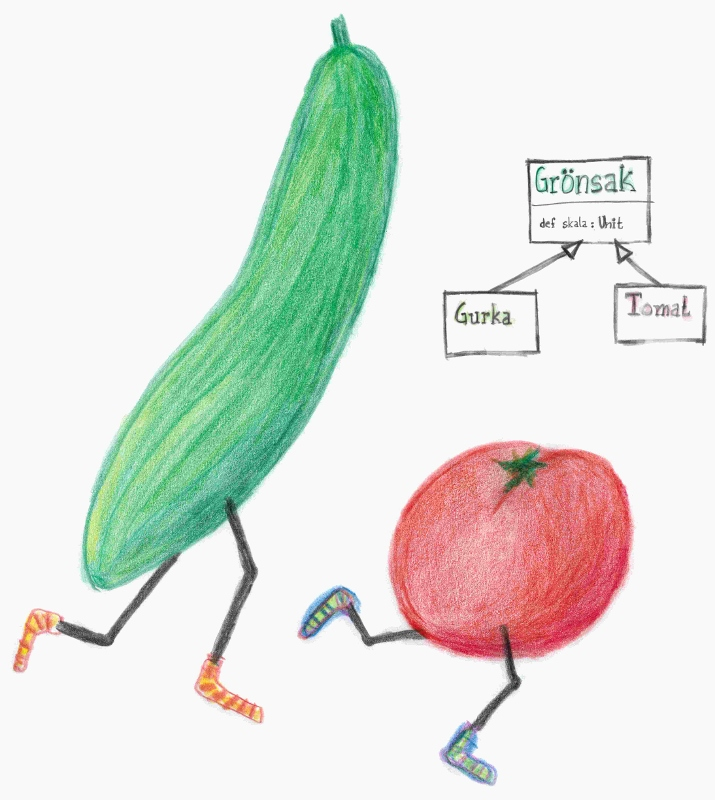
\includegraphics[width=1.5\textwidth]{../img/gurka-tomat-715x800}
\end{minipage}
\end{Slide}


\begin{Slide}{Varför behövs arv?}
\begin{itemize}
\item Man kan använda arv för att dela upp kod i:
\begin{itemize}
\item \Emph{generella} (gemensamma) delar och
\item \Emph{specifika} (specialanpassade) delar.
\end{itemize}

\item Man kan åstadkomma \Emph{kontrollerad flexibilitet}:
\begin{itemize}
\item Klientkod kan \Emph{utvidga} \Eng{extend} ett givet API med egna specifika tillägg.
\end{itemize}

\item Man kan använda arv för att deklarera en gemensam \Emph{bastyp} så att generiska samlingar kan ges en mer specifik elementtyp.
\begin{itemize}
\item Det räcker att man vet bastypen för att kunna anropa gemensamma metoder på alla element i samlingen.
\end{itemize}
\end{itemize}
\end{Slide}


\begin{Slide}{Behovet av gemensam bastyp}\SlideFontSmall
\begin{REPL}
scala> class Gurka(val vikt: Int)

scala> class Tomat(val vikt: Int)

scala> val gurkor = Vector(new Gurka(200), new Gurka(300))
gurkor: scala.collection.immutable.Vector[Gurka] =
  Vector(Gurka@60856961, Gurka@2fd953a6)

scala> gurkor.map(_.vikt)
res0: scala.collection.immutable.Vector[Int] = Vector(200, 300)

scala> val grönsaker = Vector(new Gurka(200), new Tomat(42))
grönsaker: scala.collection.immutable.Vector[Object] =
  Vector(Gurka@669253b7, Tomat@5305c37d)

scala> grönsaker.map(_.vikt)
<console>:15: error: value vikt is not a member of Object
       grönsaker.map(_.vikt)
\end{REPL}
Hur ordna en mer specifik typ än \code{Vector[Object]}? \pause$\rightarrow$ Skapa en \Emph{bastyp}!
\end{Slide}




\begin{Slide}{Skapa en gemensam bastyp}
Typen \textit{\textbf{\texttt{Grönsak}}} är en \Emph{bastyp} i nedan arvshierarki:

\vspace{1em}
\begin{center}
\newcommand{\TextBox}[1]{\raisebox{0pt}[1em][0.5em]{#1}}
\tikzstyle{umlclass}=[rectangle, draw=black,  thick, anchor=north, text width=2cm, rectangle split, rectangle split parts = 3]
\begin{tikzpicture}[inner sep=0.5em]
\node [umlclass, rectangle split parts = 1, xshift=0cm] (BaseType)  {
            \textit{\textbf{\centerline{\TextBox{\code{Grönsak}}}}}
            %\nodepart[]{second}\TextBox{\code{val vikt: Int}}
        };

\node [umlclass, rectangle split parts = 1]  at (2cm,-2cm) (SubType1) {
            \textbf{\centerline{\TextBox{\code{Gurka}}}}
            %\nodepart[]{second} \TextBox{~}
        };

\node [umlclass, rectangle split parts = 1] at (-2cm,-2cm) (SubType2)  {
            \textbf{\centerline{\TextBox{\code{Tomat}}}}
            %\nodepart[]{second} \TextBox{talk(): void}
        };
\draw[umlarrow] (SubType1.north) -- ++(0,0.5) -| (BaseType.south);
\draw[umlarrow] (SubType2.north) -- ++(0,0.5) -| (BaseType.south);
\end{tikzpicture}

\pause
\vspace{2em} Pilen ~ \tikz\draw[umlarrow] (0,0) -- (0,0.5); ~ betecknar \Emph{arv} och utläses ''\Alert{är en}''

\pause
{\vspace{1em}\SlideFontSmall Typerna \code{Tomat} och \code{Gurka} är \Emph{subtyper} till den \Emph{abstrakta} typen \code{Grönsak}.}
\end{center}
\end{Slide}







\begin{Slide}{Skapa en gemensam bastyp med \texttt{trait} och \texttt{extends}}\SlideFontSmall
Med \code{trait Grönsak} kan klasserna \code{Gurka} och \code{Tomat} få en gemensam \Emph{bastyp} genom att båda \Emph{subtyperna} gör \code{extends Grönsak}:
\begin{REPL}
scala> trait Grönsak

scala> class Gurka(val vikt: Int) extends Grönsak

scala> class Tomat(val vikt: Int) extends Grönsak

scala> val grönsaker = Vector(new Gurka(200), new Tomat(42))
grönsaker: scala.collection.immutable.Vector[Grönsak] =
  Vector(Gurka@3dc4ed6f, Tomat@2823b7c5)


\end{REPL}
\pause
Men det är fortfarande inte som vi vill ha det:
\begin{REPLnonum}
scala> grönsaker.map(_.vikt)
<console>:15: error: value vikt is not a member of Grönsak
       grönsaker.map(_.vikt)
\end{REPLnonum}
\end{Slide}



\begin{Slide}{En gemensam bastyp med gemensamma delar}\SlideFontSmall
Placera gemensamma medlemmar i bastypen:

\vspace{1em}
\begin{center}
\newcommand{\TextBox}[1]{\raisebox{0pt}[1em][0.5em]{#1}}
\tikzstyle{umlclass}=[rectangle, draw=black,  thick, anchor=north, text width=3cm, rectangle split, rectangle split parts = 3]
\begin{tikzpicture}[inner sep=0.5em]
\node [umlclass, rectangle split parts = 2, xshift=0cm] (BaseType)  {
            \textit{\textbf{\centerline{\TextBox{\code{Grönsak}}}}}
            \nodepart[]{second}\TextBox{\code{val vikt: Int}}
        };

\node [umlclass, rectangle split parts = 1]  at (2cm,-3cm) (SubType1) {
            \textbf{\centerline{\TextBox{\code{Gurka}}}}
            %\nodepart[]{second} \TextBox{~}
        };

\node [umlclass, rectangle split parts = 1] at (-2cm,-3cm) (SubType2)  {
            \textbf{\centerline{\TextBox{\code{Tomat}}}}
            %\nodepart[]{second} \TextBox{talk(): void}
        };
\draw[umlarrow] (SubType1.north) -- ++(0,0.5) -| (BaseType.south);
\draw[umlarrow] (SubType2.north) -- ++(0,0.5) -| (BaseType.south);
\end{tikzpicture}
\end{center}
\vspace{2em}
\begin{itemize}
\item Alla grönsaker har attributet \code{val vikt}.
\item Det specifika värdet på vikten definieras \Alert{inte} i bastypen.
\item Medlemen \code{vikt} kallas  \Emph{abstrakt} eftersom den \Alert{saknar implementation}.
\end{itemize}
\end{Slide}





\begin{Slide}{Placera gemensamma delar i bastypen}

Vi inkluderar det gemensamma attributet \code{val vikt} som en \Emph{abstrakt medlem} i bastypen:

\begin{Code}
trait Grönsak { val vikt: Int }

class Gurka(val vikt: Int) extends Grönsak

class Tomat(val vikt: Int) extends Grönsak
\end{Code}
Nu vet kompilatorn att alla grönsaker har en vikt:
\begin{REPL}
scala> val grönsaker = Vector(new Gurka(200), new Tomat(42))
grönsaker: scala.collection.immutable.Vector[Grönsak] =
  Vector(Gurka@3dc4ed6f, Tomat@2823b7c5)

scala> grönsaker.map(_.vikt)
res0: scala.collection.immutable.Vector[Int] = Vector(200, 42)
\end{REPL}

\end{Slide}





\begin{Slide}{Scalas typhierarki och typen \texttt{Object}}
Den översta delen av typhierarkin i Scala:
\vspace{1em}
\begin{center}
\newcommand{\TextBox}[1]{\raisebox{0pt}[1em][0.5em]{#1}}
\tikzstyle{umlclass}=[rectangle, draw=black,  thick, anchor=north, text width=2.5cm, rectangle split, rectangle split parts = 3]
\begin{tikzpicture}[inner sep=0.5em]
\node [umlclass, rectangle split parts = 1, xshift=0cm] (BaseType)  {
            \textit{\textbf{\centerline{\TextBox{\code{Any}}}}}
            %\nodepart[]{second}\TextBox{\code{def toString: String}}
        };

\node [umlclass, rectangle split parts = 1]  at (2cm,-2cm) (SubType1) {
            \textit{\textbf{\centerline{\TextBox{\code{AnyRef}}}}}
            %\nodepart[]{second} \TextBox{~}
        };

\node [umlclass, rectangle split parts = 1] at (-2cm,-2cm) (SubType2)  {
            \textit{\textbf{\centerline{\TextBox{\code{AnyVal}}}}}
            %\nodepart[]{second} \TextBox{talk(): void}
        };
\draw[umlarrow] (SubType1.north) -- ++(0,0.5) -| (BaseType.south);
\draw[umlarrow] (SubType2.north) -- ++(0,0.5) -| (BaseType.south);
\end{tikzpicture}
\end{center}
\begin{itemize}\SlideFontSmall
\item De numeriska typerna \code{Int}, \code{Double}, etc är subtyper till \Emph{\code{AnyVal}} och kallas \Emph{värdetyper} och lagras på ett speciellt, effektivt sätt i minnet.
\item Alla dina egna klasser är subtyper till \Emph{\texttt{AnyRef}} och kallas \Emph{referenstyper} och kräver (direkt eller indirekt) konstruktion med \code{new}.
\item \texttt{AnyRef} motsvaras av \Alert{\code{java.lang.Object}} i JVM.
\end{itemize}
\end{Slide}



\begin{Slide}{Implicita supertyper till dina egna klasser}
Alla dina egna typer ingår underförstått i Scalas typhierarki:

\vspace{1em}
\begin{center}
\newcommand{\TextBox}[1]{\raisebox{0pt}[1em][0.5em]{#1}}
\tikzstyle{umlclass}=[rectangle, draw=black,  thick, anchor=north, text width=2cm, rectangle split, rectangle split parts = 3]
\begin{tikzpicture}[inner sep=0.5em, scale=0.8, every node/.style={scale=0.8}]
\node [umlclass, rectangle split parts = 1, xshift=0cm] at (0,-0.3cm)(BaseType)  {
            \textit{\textbf{\centerline{\TextBox{\code{Any}}}}}
            %\nodepart[]{second}\TextBox{\code{def toString: String}}
        };

\node [umlclass, rectangle split parts = 1]  at (2cm,-2cm) (SubType1) {
            \textit{\textbf{\centerline{\TextBox{\code{AnyRef}}}}}
            %\nodepart[]{second} \TextBox{~}
        };

\node [umlclass, rectangle split parts = 1] at (-2cm,-2cm) (SubType2)  {
            \textit{\textbf{\centerline{\TextBox{\code{AnyVal}}}}}
            %\nodepart[]{second} \TextBox{talk(): void}
        };


\node [umlclass, rectangle split parts = 1] at (2cm,-3.5cm) (SubSubType)  {
            \textit{\textbf{\centerline{\TextBox{\code{Grönsak}}}}}
            %\nodepart[]{second} \TextBox{talk(): void}
        };

\node [umlclass, rectangle split parts = 1] at (3.5cm,-5.25cm) (SubSubSubType1)  {
            \textbf{\centerline{\TextBox{\code{Gurka}}}}
            %\nodepart[]{second} \TextBox{talk(): void}
        };

\node [umlclass, rectangle split parts = 1] at (0.5cm,-5.25cm) (SubSubSubType2)  {
            \textbf{\centerline{\TextBox{\code{Tomat}}}}
            %\nodepart[]{second} \TextBox{talk(): void}
        };


\draw[umlarrow] (SubType1.north) -- ++(0,0.3) -| (BaseType.south);
\draw[umlarrow] (SubType2.north) -- ++(0,0.3) -| (BaseType.south);
\draw[umlarrow] (SubSubType.north) -- (SubType1.south);
\draw[umlarrow] (SubSubSubType1.north) -- ++(0,0.3) -| (SubSubType.south);
\draw[umlarrow] (SubSubSubType2.north) -- ++(0,0.3) -| (SubSubType.south);
\end{tikzpicture}
\end{center}
\end{Slide}


\begin{Slide}{Vad är en trait?}
\begin{itemize}
\item \Alert{Trait} betyder \Emph{egenskap} på engelska.

\item En trait liknar en klass, \Alert{men} speciella regler gäller:

\begin{itemize}

\item den \Emph{kan} innehålla delar som \Emph{saknar implementation}

\item den \Emph{kan mixas} med flera andra traits så att olika koddelar kan återanvändas på flexibla sätt.

\item den \Alert{kan inte} instansieras direkt som den är.

\item den \Alert{kan inte} ha klassparametrar eller konstruktorer.
\end{itemize}

\pause
\item {\SlideFontSmall Jämförelse med Java:}
\begin{itemize}\SlideFontTiny
\item En Scala-trait liknar det som i Java kallas \jcode{interface}, men man kan göra mer med Scala-traits: färre begränsningar, fler abstraktionsmöjligheter.

\item En Scala-trait med enbart abstrakta medlemmar kompileras till bytekod i JVM:en som kan användas från Java-kod precis som ett Java-interface.
\end{itemize}
\end{itemize}

\end{Slide}

\begin{Slide}{Vad används en trait till?}
En \code{trait} används för att skapa en bastyp som kan vara hemvist för gemensamma delar hos subtyper:
\begin{Code}
trait Bastyp { val x = 42 }                 // Bastyp har medlemmen x
class Subtyp1 extends Bastyp { val y = 43 } // Subtyp1 ärver x, har även y
class Subtyp2 extends Bastyp { val z = 44 } // Subtyp2 ärver x, har även z
\end{Code}
\pause\vspace{-0.5em}
\begin{REPL}
scala> val a = new Subtyp1
a: Subtyp1 = Subtyp1@51016012

scala> a.x
res0: Int = 42

scala> a.y
res1: Int = 43

scala> a.z
<console>:15: error: value z is not a member of Subtyp1

scala> new Bastyp
<console>:13: error: trait Bastyp is abstract; cannot be instantiated
\end{REPL}

\end{Slide}


\begin{Slide}{En trait kan ha abstrakta medlemmar}
\begin{Code}
trait X { val x: Int }   // x är abstrakt, d.v.s. saknar implementation
class A extends X { val x = 42 }   // x ges en implementation
class B extends X { val x = 43 }   // x ges en annan implementation
\end{Code}
\pause\vspace{-0.5em}
\begin{REPL}
scala> val a = new A
a: A = A@5faeada1

scala> val b = new B
b: B = B@cb51256

scala> val xs = Vector(a,b)
xs: scala.collection.immutable.Vector[X] = Vector(A@5faeada1, B@cb51256)

scala> xs.map(_.x)
res0: scala.collection.immutable.Vector[Int] = Vector(42, 43)

scala> class Y { val y: Int }
  error: class Y needs to be abstract, since value y is not defined

scala> trait Z(x: Int)
  error: traits or objects may not have parameters

\end{REPL}
\end{Slide}


\begin{Slide}{Terminologi och nyckelord vid arv}\SlideFontTiny

\begin{tabular}{r  l}
\Emph{subtyp}           & en typ som ärver en supertyp\\
\Emph{supertyp}         & en typ som ärvs av en subtyp\\
\Emph{bastyp}           & en typ som är rot i ett arvsträd\\
\Emph{abstrakt medlem}  & en medlem som saknar implementation\\
\Emph{konkret medlem}   & en medlem som ej saknar implementation\\
\Emph{abstrakt typ}     & en typ som kan ha abstrakta medlemmar; kan ej instansieras\\
\Emph{konkret typ}      & en typ som ej har abstrakta medlemmar; kan instansieras\\
\code|class|            & en klass är en konkret typ: \Alert{kan ej ha abstrakta medlemmar}\\
\code|abstract class|   & en klass är en abstrakt typ som \Emph{kan ha parametrar}\\
\code|trait|            & är en abstrakt typ, \Alert{kan ej ha parametrar} men \Emph{kan mixas in}\\
\code|extends|          & står före en supertyp, medför arv av supertypens medlemmar\\
\code|override|         & en medlem överskuggar (byter ut) en medlem i en superttyp\\
\code|protected|        & gör en medlem synlig i subtyper till denna typ (jmf \code|private|)\\
\code|final gurka|      & gör medlemen gurka final: förhindrar överskuggning\\
\code|final class|      & gör klassen final: förhindrar vidare subtypning\\
\code|sealed trait|     & förseglad trait: bara de direkta subtyperna i denna kodfil\\
\code|super.gurka|      & refererar till supertypens medlem \code|gurka| (jmf \code|this|)\\
\end{tabular}

\ifkompendium\else
\pause
\begin{tikzpicture}[overlay]
     \node at (10.7,0.6) {
\includegraphics[scale=0.36]{../img/ttsuper}};
\end{tikzpicture}
\fi

\end{Slide}


\begin{Slide}{Abstrakta och konkreta medlemmar}
\vspace{-0.5em}\scalainputlisting[numbers=left,numberstyle=,basicstyle=\fontsize{6}{7}\ttfamily\selectfont]{../compendium/examples/workspace/w07-inherit/src/vego1.scala}
\end{Slide}


\begin{Slide}{Undvika kodduplicering med hjälp av arv}
\scalainputlisting[numbers=left,numberstyle=,basicstyle=\fontsize{6}{7.3}\ttfamily\selectfont]{../compendium/examples/workspace/w07-inherit/src/vego2.scala}
\end{Slide}




\begin{Slide}{Varför kan kodduplicering orsaka problem?}
\begin{itemize}
\item Mer att skriva (inte jättestort problem)
\pause
\item Fler kodrader att läsa och förstå
\pause
\item Fler kodrader som påverkas vid tillägg
\pause

\item Fler kodrader att underhålla:
\begin{itemize}
\item Om man rättar en bug på ett ställe måste man komma ihåg att göra \Alert{exakt samma ändring} på alla de ställen där kodduplicering förekommer $\rightarrow$ \Alert{risk för nya buggar}
\end{itemize}

\pause

\item Principen på engelska: \code{ DRY == "Don't Repeat Yourself!"}

\pause

\item {Men det kan finnas tillfällen när kodduplicering faktiskt är att föredra: t.ex. om man vill att olika delar av koden ska vara helt oberoende av varandra.}
\end{itemize}
\end{Slide}




\begin{Slide}{Överskuggning}
\vspace{-0.5em}\scalainputlisting[numbers=left,numberstyle=,basicstyle=\fontsize{6}{7.3}\ttfamily\selectfont]{../compendium/examples/workspace/w07-inherit/src/vego3.scala}
\end{Slide}

\begin{Slide}{En final medlem kan ej överskuggas}
\vspace{-0.5em}\scalainputlisting[numbers=left,numberstyle=,basicstyle=\fontsize{6}{7.3}\ttfamily\selectfont]{../compendium/examples/workspace/w07-inherit/src/vego4.scala}
\end{Slide}


\begin{Slide}{Protected ger synlighet begränsad till subtyper}
\begin{REPL}
scala> trait Super {
         private val minHemlis = 42
         protected val vårHemlis = 42
       }

scala> class Sub extends Super { def avslöjad = minHemlis }
error: not found: value minHemlis

scala> class Sub extends Super { def avslöjad = vårHemlis }

scala> val s = new Sub
s: Sub = Sub@2eee9593

scala> s.avslöjad
res0: Int = 42

scala> s.minHemlis
error: value minHemlis is not a member of Sub

scala> s.vårHemlis
error: Access to protected value vårHemlis not permitted
\end{REPL}
\end{Slide}


\begin{Slide}{Filnamnsregler och -konventioner}
\begin{itemize}
\item Java
\begin{itemize}
\item I Java får man bara ha \Alert{en enda} publik klass per kodfil.
\item I Java måste kodfilen ha \Alert{samma namn} som den publika klassen, t.ex. \code{KlassensNamn.java}
\end{itemize}
\item Scala
\begin{itemize}
\item I Scala får man ha \Emph{många} klasser/traits/singelobjekt i samma kodfil.
\item I Scala får man döpa kodfilerna \Emph{oberoende} av deras innehåll. \pause Dessa \Emph{konventioner} används:
\begin{itemize}
\item Om en kodfil bara innehåller \Emph{en enda} klass/trait/singelobjekt ge filen samma namn som innehållet, t.ex. \code{KlassensNamn.scala}
\item Om en kodfil innehåller \Emph{flera} saker, döp filen till något som återspeglar hela innehållet och använd \Emph{liten begynnelsebokstav}, t.ex. \code{drawing.scala} eller \code{bastypensNamn.scala}
\end{itemize}


\end{itemize}

\end{itemize}
\end{Slide}


\begin{Slide}{Klasser, arv och klassparametrar}\SlideFontTiny
Klasser kan ärva klasser. Om superklassen har klassparametrar måste primärkonstruktor ges argument efter \code{extends}.

\scalainputlisting[numbers=left,numberstyle=,basicstyle=\fontsize{6.4}{7.7}\ttfamily\selectfont]{../compendium/examples/workspace/w07-inherit/src/personExample1.scala}

\end{Slide}


\begin{Slide}{Statisk och dynamisk typ}\SlideFontSmall
\begin{Code}
    var p: Person = new Forskare("Robin Smith", "Lund", "Professor Dr")
\end{Code}
\begin{itemize}
\item Den \Emph{statiska typen} för \code{p} är \code{Person} vilket gör att vi sedan kan låta \code{p} referera till andra instanser som är av typen Person.
\begin{Code}
p = new Student("Kim Robinson", "Lund", "Data")
\end{Code}

\pause

\item Med ''statisk typ'' menas den typinformation som kompilatorn känner till vid kompileringstid.

\pause
\item Den \Emph{dynamiska typen}, även kallad \Emph{körtidstypen}, som gäller under körning är här mer specifik och mångfaceterad: \code{p} är efter tilldelning nu Student, Person och Akademiker (men inte Examinerad).

\pause

\item Man kan undersöka om den dynamiska typen för \code{p} är \code{EnVissTyp} med  \code{p.isInstanceOf[EnVissTyp]}

\pause

\item Man kan säga åt kompilatorn: \emph{''jag garanterar att p är av typen \code{EnVissTyp} så du kan omforma den till \code{EnVissTyp}''} med  \code{p.asInstanceOf[EnVissTyp]} \\ \pause (detta är inte så vanligt i normal Scala-kod)
\end{itemize}
\end{Slide}




\begin{Slide}{Inmixning}\SlideFontTiny
Man kan ärva flera traits. Detta kallas inmixning \Eng{mix-in} och görs med \code{with}.
\scalainputlisting[numbers=left,numberstyle=,basicstyle=\fontsize{6.4}{7.7}\ttfamily\selectfont]{../compendium/examples/workspace/w07-inherit/src/personExample2.scala}
\end{Slide}



\begin{Slide}{\texttt{isInstanceOf} och \texttt{asInstanceOf}}\SlideFontTiny
Testa körtidstyp med \code{isInstanceOf[Typ]}. Lova kompilatorn (och ta själv ansvar för) att det är en viss körtidstyp med \code{asInstanceOf[Typ]}. OBS! Använd hellre \code{match}.
\scalainputlisting[basicstyle=\small\SlideFontSize{6.2}{7.6}\ttfamily\selectfont]{../compendium/examples/workspace/w07-inherit/src/personExample3.scala}
\end{Slide}



\begin{Slide}{Polymorfism och dynamisk bindning}\SlideFontTiny
\begin{Code}[basicstyle=\SlideFontSize{6.2}{7.5}\ttfamily\selectfont]
trait Robot { def work(): Unit }

case class CleaningBot(name: String) extends Robot {
  override def work(): Unit = println(" Städa Städa")
}

case class TalkingBot(name: String) extends Robot {
  override def work(): Unit = println(" Prata Prata")
}
\end{Code}
\Emph{Polymorfism} betyder ''många former''. Referenserna r och bot nedan kan ha olika ''former'', d.v.s de kan referera till olika sorters robotar. \\ \Emph{Dynamisk bindning} innebär att körtidstypen avgör vilken metod som körs.
\begin{REPL}[numbers=left, basicstyle=\color{white}\SlideFontSize{6.2}{7.5}\ttfamily\selectfont]
scala> def robotDoWork(bot: Robot) = { print(bot); bot.work }

scala> var r: Robot = new CleaningBot("Wall-E")

scala> robotDoWork(r)
CleaningBot(Wall-E) Städa Städa

scala> r = new TalkingBot("C3PO")

scala> robotDoWork(r)
TalkingBot(C3PO) Prata Prata
\end{REPL}
\end{Slide}


\begin{Slide}{Anonym klass}
Om man har en abstrakt typ med saknade implementationer kan man fylla i det som fattas i dessa i ett extra block som ''hängs på'' vid instansiering:
\begin{REPL}
scala> trait Grönsak { val vikt: Int }
defined trait Grönsak

scala> new Grönsak
<console>:13: error: trait Grönsak is abstract; cannot be instantiated
       new Grönsak
       ^

scala> new Grönsak { val vikt = 42 }
res0: Grönsak = $anon$1@4e3f2908
\end{REPL}
Man får då vad som kallas en \Emph{anonym klass}. (I detta fall en ganska konstig grönsak som inte är någon speciell sorts grönsak med som ändå har en vikt.)
\end{Slide}


\Subsection{Uppräknade värden}


\begin{Slide}{Uppräknade värden med heltal}\SlideFontSmall
Vi kan använda heltalskonstanter för att representera olika färger.
\begin{Code}
object Färg {
  val Spader = 1
  val Hjärter = 2
  val Ruter = 3
  val Klöver = 4
}
\end{Code}
\begin{Code}[language=,keywords={case,class}]
case class Kort(färg: Int, valör: Int)
\end{Code}

Vi kan nu använda våra uppräknade färgvärden så här:
\begin{REPLnonum}
scala> import Färg._
scala> Kort(Ruter, 7)
\end{REPLnonum}
\pause Men kompilatorn \Alert{kan inte hindra} denna bugg:
\begin{REPLnonum}
scala> Kort(42, 7)
\end{REPLnonum}

\end{Slide}


\begin{Slide}{Uppräknade värden med case-objekt}\SlideFontSmall
Vi kan använda case-objekt för att representera olika färger.
\begin{Code}[language=,keywords={sealed,trait,object,case,class,extends}]
sealed trait Färg
case object Spader  extends Färg
case object Hjärter extends Färg
case object Ruter   extends Färg
case object Klöver  extends Färg

case class Kort(färg: Färg, valör: Int)
\end{Code}

Vi kan nu använda våra uppräknade färgvärden så här:
\begin{REPL}
scala> Kort(Ruter, 7)

scala> Kort(Spader, 1)
\end{REPL}
\begin{itemize}
\item Kompilatorn \Emph{garanterar} att vi bara använder exakt dessa färger.

\item Nyckelordet \code{sealed} förhindrar fler subtyper förutom de som finns här.

\item \code{case} före \code{object} ger en najs \code{toString} och möjliggör matchning \\
(mer om matchning i w10).

\end{itemize}

\end{Slide}

\begin{Slide}{Uppräknade värden i samling}\SlideFontSmall
Vi kan placera case-objekten i en samling som kan användas i loopar. \\ Ett lämpligt ställe för en sådan samling är i kompanjonsobjektet till \code{Färg}.
\begin{Code}
sealed trait Färg
object Färg {
  val values = Vector(Spader, Hjärter, Ruter, Klöver)
}
case object Spader extends Färg
case object Hjärter extends Färg
case object Ruter extends Färg
case object Klöver extends Färg
\end{Code}

\begin{REPL}
scala> val allaEss = for (f <- Färg.values) yield Kort(f, 1)
\end{REPL}
\end{Slide}


\begin{Slide}{Uppräknade värden med heltalsomvandling}\SlideFontSmall
Med en \code{sealed abstract class} och ett heltalsattrribut \code{toInt} som klassparameter kan vi erbjuda omvandling till heltal.
\begin{Code}
sealed abstract class Färg(final val toInt: Int)
object Färg {
  val values = Vector(Spader, Hjärter, Ruter, Klöver)
}
case object Spader  extends Färg(0)
case object Hjärter extends Färg(1)
case object Ruter   extends Färg(2)
case object Klöver  extends Färg(3)
\end{Code}

\begin{REPL}
scala> Kort(Ruter, 1).färg.toInt
res0: Int = 2
\end{REPL}
Nyckelordet \code{abstract} förhindrar instansiering av \code{Färg}. \\
Nyckelordet \code{final} förhindrar överskuggning av attributet \code{toInt}. \\
Nyckelordet \code{sealed} förhindrar vidare subtypning av \code{Färg}.
\end{Slide}



\Subsection{Exempel: Shape}


\begin{Slide}{Exempel: shapes1.scala}
Typisk Scala-kod: En trait som bastyp åt flera case-klasser.
\scalainputlisting[numbers=left,numberstyle=,basicstyle=\fontsize{6.4}{7.7}\ttfamily\selectfont]{../compendium/examples/workspace/w07-inherit/src/shapes1.scala}
\end{Slide}

\begin{Slide}{Exempel: shapesTest1.scala}
Test av konkreta subklasser till bastypen \code{Shape}.
\scalainputlisting[numbers=left,numberstyle=,basicstyle=\fontsize{6.4}{7.7}\ttfamily\selectfont]{../compendium/examples/workspace/w07-inherit/src/shapesTest1.scala}

\begin{REPL}
Rectangle((100.0,100.0),(75.0,120.0))
Rectangle((141.0,183.0),(75.0,120.0))
Triangle((0.0,0.0),(4.0,0.0),(4.0,3.0))
Triangle((1.0,1.0),(4.0,0.0),(4.0,3.0))
Triangle((0.0,0.0),(4.0,0.0),(4.0,3.0))
\end{REPL}
\end{Slide}


\begin{Slide}{Fördjupningsexempel gränssnitt: draw.scala}
Två traits som kan användas för att ''koppla ihop'' kod och ge flexibilitet i implementationen:
\scalainputlisting[%numbers=left,numberstyle=,
basicstyle=\fontsize{9}{11}\ttfamily\selectfont]{../compendium/examples/workspace/w07-inherit/src/draw.scala}

\pause
\setlength{\leftmargini}{0pt}
\begin{itemize}\SlideFontSmall
\item  Traits som använda för att abstrahera implementation och möjliggöra uppfyllandet av ett slags ''kontrakt'' om vad som ska finnas kallas \Emph{gränssnitt} \Eng{interface} och används ofta för att skapa av ett flexibelt api.

%\item Implementationen av de delar vi vill kunna ändra senare placeras i subtyper som inte används direkt av klientkoden. 

\item Vi visar bara information om vad som erbjuds men inte hur det ser ut ''inuti''.

\end{itemize}
\end{Slide}

\begin{Slide}{Exempel: shapes2.scala}\SlideFontTiny
Genom att \Emph{mixa in} vår \code{trait CanDraw} kan en rektangel nu även ritas ut:

\scalainputlisting[numbers=left,numberstyle=,basicstyle=\fontsize{6.5}{7.8}\ttfamily\selectfont]{../compendium/examples/workspace/w07-inherit/src/shapes2.scala}

\pause
\vspace{-0.5em}Notera: ingen ändring i \code {Shape}! Vi behöver nu bara ett \Emph{\code{DrawingWindow}}...
\end{Slide}


\begin{Slide}{Exempel: SimpleDrawingWindow.scala}\SlideFontTiny
\vspace{-0.35em}
Vi skapar en ny klass som ärver \code{SimpleWindow}, som \Alert{dessutom} även \Emph{är ett} \code{DrawingWindow}, tack vare \Emph{inmixning} med nyckelordet \code{with}.\\
Observera att vi måste skicka vidare klassparametrarna till superklassens konstruktor.

\scalainputlisting[numbers=left,numberstyle=,basicstyle=\fontsize{6.4}{7.7}\ttfamily\selectfont]{../compendium/examples/workspace/w07-inherit/src/SimpleDrawingWindow.scala}

\pause
\vspace{-0.35em}
\scalainputlisting[numbers=left,numberstyle=,basicstyle=\fontsize{6.4}{7.7}\ttfamily\selectfont]{../compendium/examples/workspace/w07-inherit/src/shapesTest2.scala}
\end{Slide}


%\begin{Slide}{Exempel: Robot}
%\begin{center}
%\newcommand{\TextBox}[1]{\raisebox{0pt}[1em][0.5em]{#1}}
%\begin{tikzpicture}[inner sep=0.5em]
%\node [umlclass, rectangle split parts = 2, xshift=0cm] (AbstractRobot)  {
%            \textit{\textbf{\centerline{\TextBox{AbstractRobot}}}}
%            \nodepart[]{second}\TextBox{work(): void}
%        };
%
%\node [umlclass, rectangle split parts = 2]  at (2cm,-3cm) (MuteRobot) {
%            \textbf{\centerline{\TextBox{MuteRobot}}}
%            \nodepart[]{second} \TextBox{~}
%        };
%
%\node [umlclass, rectangle split parts = 2] at (-2cm,-3cm) (TalkingRobot)  {
%            \textbf{\centerline{\TextBox{TalkingRobot}}}
%            \nodepart[]{second} \TextBox{talk(): void}
%        };
%\draw[umlarrow] (TalkingRobot.north) -- ++(0,0.5) -| (AbstractRobot.south);
%\draw[umlarrow] (MuteRobot.north) -- ++(0,0.5) -| (AbstractRobot.south);
%\end{tikzpicture}
%\end{center}
%\end{Slide}






\begin{Slide}{Attribut och metoder i UML-diagram}
\begin{center}
\begin{tikzpicture}
\node (Class) [umlclass, rectangle split parts = 3, xshift = -2cm, yshift=-1.5cm, text width = 4.2cm, scale=0.8]  {
            \textbf{\centerline{Name}}
            \nodepart[]{second}attr1: Type \newline attr2: Type
            \nodepart[]{third}method1(a: Type): Type \newline  method2(b: Type): Type
       };
\node (explain1)[above of = Class, yshift=1cm, text width=4.9cm]{En klass i ett \Emph{UML}-diagram kan ha 3 delar:};
\node (explain2)[below of = Class, yshift=-1cm]{Ibland utelämnar man typerna.};



\node [umlclass, rectangle split parts = 3]  at (4,0) (Robot) {
            \textbf{\centerline{Robot}}
            \nodepart[]{second}name: String
            \nodepart[]{third}work(): Unit
       };
\node [umlclass, rectangle split parts = 3]  at (4, -3) (TalkingRobot)  {
            \textbf{\centerline{TalkingRobot}}
            \nodepart[]{second} phrase: String
            \nodepart[]{third}speak(): Unit
        };
\draw[umlarrow] (TalkingRobot.north) -- ++(0,0.8) -| (Robot.south);
\end{tikzpicture}
\end{center}
\hskip2em\href{https://en.wikipedia.org/wiki/Class_diagram}{\SlideFontTiny en.wikipedia.org/wiki/Class\_diagram}
\end{Slide}

%!TEX encoding = UTF-8 Unicode
%!TEX root = ../lect-w09.tex

%%%


%\begin{Slide}{TODO: Begrepp att förklara}
%  Tänk igenom ordningen:
%  \begin{itemize}
%    \item OO, arv, supertyp, subtyp, bastyp, polymorfism, ... 
%  \end{itemize}
%\end{Slide}


\Subsection{Överskuggingsregler}

\begin{Slide}{Medlemmar, arv och överskuggning}\SlideFontTiny
\begin{multicols}{2}
Olika sorters överskuggningsbara medlemmar i klasser och traits i \Emph{Scala}:
\begin{itemize}
\item \code{def}
\item \code{val}
\item \code{lazy val}
\item \code{var}
\end{itemize}


\columnbreak

\pause

Olika sorters överskuggningsbara instansmedlemmar i \Emph{Java}:
\begin{itemize}
\item variabel 
\item metod
\end{itemize}

{\SlideFontTiny Medlemmar som är \jcode{static} kan ej överskuggas (men döljas) vid arv.}

\vspace{0.5em}
\end{multicols}

\pause
\begin{itemize}\SlideFontTiny
\item När man överskuggar \Eng{override} en medlemmen med en annan medlem med samma namn i en subtyp, får denna medlem en (ny) implementation. 

\item När man konstruerar ett objektorienterat språk gäller det att man definierar sunda överskuggningsregler vid arv. Detta är förvånansvärt knepigt.

\item Singelobjekt kan ej ärvas (och medlemmar i singelobjekt kan därmed ej överskuggas).
\end{itemize}
\end{Slide}


\begin{Slide}{Fördjupning: Regler för överskuggning i Scala} \SlideFontTiny
\label{slideW07:overriderules}
En medlem M1 i en supertyp får överskuggas av en medlem M2 i en subtyp, enligt dessa regler:
\begin{enumerate}
\item M1 och M2 ska ha samma namn och typerna ska matcha.
\item \code{def} får bytas ut mot: \code{def}, \code{val}, \code{var}, \code{lazy val}
\item \code{val} får bytas ut mot: \code{val}, och om M1 är abstrakt mot en \code{lazy val}.
\item \code{var} får bara bytas ut mot en \code{var}.
\item \code{lazy val} får bara bytas ut mot en \code{lazy val}.
\item Om en medlem i en supertyp är abstrakt \emph{behöver} man inte använda nyckelordet \code{override} i subtypen. (Men det är bra att göra det ändå så att kompilatorn hjälper dig att kolla att du verkligen överskuggar något.) 
\item Om en medlem i en supertyp är konkret \emph{måste} man använda nyckelordet \code{override} i subtypen, annars ges kompileringsfel.
\item M1 får inte vara \code{final}.
\item M1 får inte vara \code{private} eller \code{private[this]}, men kan vara \code{private[X]} om M2 också är \code{private[X]}, eller \code{private[Y]} om X innehåller Y.   
\item Om M1 är \code{protected} måste även M2 vara det.

\end{enumerate}
\end{Slide}


\begin{Slide}{Fördjupning: Regler för överskuggning i Java}
\url{http://docs.oracle.com/javase/tutorial/java/IandI/override.html}
\end{Slide}


\Subsection{\texttt{super}}

\begin{Slide}{Att skilja på mitt och ditt med \texttt{super}}
\begin{REPL}
scala> class X { val gurka = "super pepinos" }

scala> class Y extends X { 
         override val gurka = ":("
         val sg = super.gurka 
       }

scala> val y = new Y
y: Y = Y@26ba2a48

scala> y.gurka
res0: String = :(
\end{REPL}
Super Pepinos to the rescue:
\pause
\begin{REPLnonum}
scala> y.sg
res1: String = super pepinos

\end{REPLnonum}


\pause
\begin{tikzpicture}[overlay]
     \node at (7.5,1.7) {
\includegraphics[scale=0.5]{../img/ttsuper}};
\end{tikzpicture}
\href{http://www.pepinadas.com/tirassuper1.html}{\small www.pepinadas.com/tirassuper1.html}
\end{Slide}





\Subsection{Trait eller abstrakt klass?}

\begin{Slide}{Trait eller abstrakt klass?} 
\SlideFontSmall
\label{slideW07:traitorclass}
\begin{multicols}{2}
Använd en \Emph{trait} som supertyp om...
\begin{itemize}
\item ...du är osäker på vilket som är bäst. (Du kan alltid ändra till en abstrakt klass senare.)
\item ...du vill kunna mixa in din trait tillsammans med andra traits.
\item ...du bara har abstrakta medlemmar. 
\end{itemize}

\columnbreak

Använd en \Alert{abstrakt klass} som supertyp om...
\begin{itemize}
\item ...du vill ge supertypen en parameter vid konstruktion.
\item ...du vill ärva supertypen från klasser skrivna i Java.
\item ...du vill minimera vad som behöver omkompileras vid ändringar. 
\end{itemize}


\end{multicols}
\end{Slide}





%\begin{Slide}{Designexempel: Klassen ???}\small
%TODO:
%  \begin{itemize} 
%  \item 
%  \end{itemize}
%\end{Slide}











%\chapter{Sökning, Sortering}\label{chapter:W10}
\begin{itemize}[nosep]
\item algoritm: LINEAR-SEARCH
\item algortim: BINARY-SEARCH
\item algoritmisk komplexitet
\item sortering till ny vektor
\item sortering på plats
\item algoritm: INSERTION-SORT
\item algoritm: SELECTION-SORT
\end{itemize}

%!TEX encoding = UTF-8 Unicode
%!TEX root = ../exercises.tex

\ifPreSolution

\Exercise{\ExeWeekTEN}\label{exe:W10}

\begin{Goals}
%!TEX encoding = UTF-8 Unicode

%!TEX root = ../compendium2.tex

\item Kunna deklarera och använda en arvshierarki i flera nivåer med nyckelordet \code{extends}.

\item Känna till synlighetsregler vid arv och nyttan med privata och skyddade medlemmar och nyckelorden \code{private} och \code{protected}.

%\item Kunna deklarera och använda skyddade medlemmar.

\item Kunna deklarera och använda överskuggade medlemmar och nyckelordet \code{override}.

\item Kunna deklarera och använda en hierarki av klasser där konstruktorparametrar överförs till superklasser.

\item Kunna deklarera och använda uppräknade värden med case-objekt och gemensam bastyp.

\item Känna till reglerna som gäller vid överskuggning av olika sorters medlemmar.

\item Känna till nyttan med finala klasser och finala attribut och nyckelordet \code{final}.

\item Kännedom om dessa begrepp:
bastyp,
sypertyp,
subtyp,
körtidstyp,
dynamisk bindning,
polymorfism,
trait,
inmixning,
överskuggad medlem,
anonym klass,
skyddad medlem,
abstrakt medlem,
abstrakt klass,
referenstyp,
värdetyp.



%TODO KOLLA PÅ NEDAN MÅL OCH BESTÄM HUR DE SKA IN I ÖVNINGARNA

%\item Känna till hur typtester och typkonvertering under körtid kan göras med metoderna \code{isInstanceOf} och \code{asInstanceOf} och känna till att detta görs bättre med \code{match}.

%\item Kunna deklarera och använda inmixning med flera traits och nyckelordet \code{with}.

%\item Kunna referera till medlem i superklassen med referensen \code{super} och känna till när detta nyckel ord behövs.

%\item Känna till begreppet anonym klass.

\end{Goals}

\begin{Preparations}
\item \StudyTheory{10}
\end{Preparations}

\BasicTasks

\else

\ExerciseSolution{\ExeWeekTEN}

\BasicTasks

\fi



\WHAT{Para ihop begrepp med beskrivning.}

\QUESTBEGIN

\Task \what

\vspace{1em}\noindent Koppla varje begrepp med den (förenklade) beskrivning som passar bäst:

\begin{ConceptConnections}
  bastyp & 1 & & A & har supertypen \code|AnyRef|, allokeras i heapen via referens \\ 
  supertyp & 2 & & B & kan ha många former, t.ex. en av flera subtyper \\ 
  subtyp & 3 & & C & klass utan namn, utvidgad med extra implementation \\ 
  körtidstyp & 4 & & D & en typ som är mer specifik \\ 
  dynamisk bindning & 5 & & E & kan ha parametrar, kan ej instansieras, kan ej mixas in \\ 
  polymorfism & 6 & & F & saknar implementation \\ 
  trait & 7 & & G & har supertypen \code|AnyVal|, lagras direkt på stacken \\ 
  inmixning & 8 & & H & tillföra egenskaper med \code|with| och en trait \\ 
  överskuggad medlem & 9 & & I & är abstrakt, kan mixas in, kan ej ha parametrar \\ 
  anonym klass & 10 & & J & kan vara mer specifik än den statiska typen \\ 
  skyddad medlem & 11 & & K & är endast synlig i subtyper \\ 
  abstrakt medlem & 12 & & L & körtidstypen avgör vilken metod som körs \\ 
  abstrakt klass & 13 & & M & medlem i subtyp ersätter medlem i supertyp \\ 
  förseglad typ & 14 & & N & den mest generella typen i en arvshierarki \\ 
  referenstyp & 15 & & O & en typ som är mer generell \\ 
  värdetyp & 16 & & P & subtypning utanför denna kodfil är förhindrad \\ 
\end{ConceptConnections}

\SOLUTION

\TaskSolved \what

\begin{ConceptConnections}
  bastyp & 1 & ~~\Large$\leadsto$~~ &  N & den mest generella typen i en arvshierarki \\ 
  supertyp & 2 & ~~\Large$\leadsto$~~ &  O & en typ som är mer generell \\ 
  subtyp & 3 & ~~\Large$\leadsto$~~ &  D & en typ som är mer specifik \\ 
  körtidstyp & 4 & ~~\Large$\leadsto$~~ &  J & kan vara mer specifik än den statiska typen \\ 
  dynamisk bindning & 5 & ~~\Large$\leadsto$~~ &  L & körtidstypen avgör vilken metod som körs \\ 
  polymorfism & 6 & ~~\Large$\leadsto$~~ &  B & kan ha många former, t.ex. en av flera subtyper \\ 
  trait & 7 & ~~\Large$\leadsto$~~ &  I & är abstrakt, kan mixas in, kan ha parametrar \\ 
  inmixning & 8 & ~~\Large$\leadsto$~~ &  H & tillföra egenskaper med \code|with| och en trait \\ 
  överskuggad medlem & 9 & ~~\Large$\leadsto$~~ &  M & medlem i subtyp ersätter medlem i supertyp \\ 
  anonym klass & 10 & ~~\Large$\leadsto$~~ &  C & klass utan namn, utvidgad med extra implementation \\ 
  skyddad medlem & 11 & ~~\Large$\leadsto$~~ &  K & är endast synlig i subtyper \\ 
  abstrakt medlem & 12 & ~~\Large$\leadsto$~~ &  F & saknar implementation \\ 
  abstrakt klass & 13 & ~~\Large$\leadsto$~~ &  E & kan ha parametrar, kan ej instansieras, kan ej mixas in \\ 
  förseglad typ & 14 & ~~\Large$\leadsto$~~ &  P & subtypning utanför denna kodfil är förhindrad \\ 
  referenstyp & 15 & ~~\Large$\leadsto$~~ &  A & har supertypen \code|AnyRef|, allokeras i heapen via referens \\ 
  värdetyp & 16 & ~~\Large$\leadsto$~~ &  G & har supertypen \code|AnyVal|, lagras direkt på stacken \\ 
\end{ConceptConnections}

\QUESTEND





\WHAT{Gemensam bastyp.}

\QUESTBEGIN

\Task  \what~  Man vill ofta lägga in objekt av olika typ i samma samling.
\begin{REPL}
scala> class Gurka(val vikt: Int)
scala> class Tomat(val vikt: Int)
scala> val gurkor = Vector(Gurka(100), Gurka(200))
scala> val grönsaker = Vector(Gurka(300), Tomat(42))
\end{REPL}

\Subtask Om en samling innehåller objekt av flera olika typer försöker kompilatorn härleda den mest specifika typen som objekten har gemensamt. Vad blir det för typ på värdet \code{grönsaker} ovan?

\Subtask Försök ta reda på summan av vikterna enligt nedan. Vad ger andra raden för felmeddelande? Varför?

\begin{REPL}
scala> gurkor.map(_.vikt).sum     // fungerar
scala> grönsaker.map(_.vikt).sum  // fungerar inte
\end{REPL}

\Subtask Du ska nu göra så att du kan komma åt vikten på alla grönsaker genom att ge gurkor och tomater en gemensam bastyp som de olika konkreta grönsakstyperna utvidgar med nyckelordet \code{extends}. Det heter att subtyperna \code{Gurka} och \code{Tomat} \textbf{ärver} egenskaperna hos supertypen \code{Grönsak}.

Skapa en bastyp \code{Grönsak} med ett abstrakt attribut \code{vikt}. Låt sedan de konkreta grönsakerna ärva bastypen:

\begin{REPL}
scala> trait Grönsak { val vikt: Int }
scala> class Gurka(val vikt: Int) extends Grönsak
scala> class Tomat(val vikt: Int) extends Grönsak
scala> val gurkor = Vector(Gurka(100), Gurka(200))
scala> val grönsaker = Vector(Gurka(300), Tomat(42))
\end{REPL}
När sker initialisering av attributet \code{vikt}?

\Subtask Vad blir det nu för typ på variabeln \code{grönsaker} ovan?

\Subtask Går det nu att summera av vikterna i \code{grönsaker} med uttrycket nedan? Varför?\\ \code{grönsaker.map(_.vikt).sum}


\Subtask En trait liknar en klass, men man kan inte instansiera den direkt. Vad blir det för felmeddelande om du försöker skapa en instans av en trait enligt nedan?
\begin{REPL}
scala> trait Grönsak { val vikt: Int }
scala> new Grönsak
\end{REPL}


\Subtask Traiten \code{Grönsak} har en abstrakt medlem \code{vikt}. Den sägs vara abstrakt eftersom den saknar definition -- medlemmen har bara ett namn och en typ men inget värde. Du kan instansiera den abstrakta traiten \code{Grönsak} om du fyller i det som ''fattas'', nämligen ett värde på \code{vikt}. Man kan fylla på det som fattas i genom att ''hänga på'' ett block efter typens namn vid instansiering. Man får då vad som kallas en \textbf{anonym klass}, i detta fall en ganska konstig grönsak som inte är någon speciell sorts grönsak med som ändå har en vikt.

Vad får \code{anonymGrönsak} nedan för typ och strängrepresenation?
\begin{REPL}
scala> val anonymGrönsak = new Grönsak { val vikt = 42 }
\end{REPL}

\Subtask Vad blir felmeddelandet om du skapar en anonym klass \code{Grönsak} med en kropp som saknar definition av vikt?

\SOLUTION


\TaskSolved \what


\SubtaskSolved  \code{Vector[Object]}. Typen \code{Object} i JVM är motsvarar typen \code{AnyRef} som är bastyp för alla referenstyper.

\SubtaskSolved  Felmeddelande:
\begin{REPLnonum}
scala> grönsaker.map(_.vikt).sum  
-- Error:                                                                                 
1 |grönsaker.map(_.vikt).sum
  |              ^^^^^^
  |             value vikt is not a member of Object - did you mean wait?
-- Error:
1 |grönsaker.map(_.vikt).sum
  |                         ^
  |ambiguous implicit arguments: both object DoubleIsFractional in object Numeric and object ShortIsIntegral in object Numeric match type Numeric[B] of parameter num of method sum in trait IterableOnceOps
\end{REPLnonum}
Det första felmeddelandet beror på att vektorns element är av typen \code{Object} och medlemmen \code{vikt} är inte definierat för denna typ. Det andra felmeddelandet är ett följdfel som beror på att en sekvens med element av typen \code{Object} inte kan summeras eftersom kompilatorn inte kan härleda att elementtypen är numerisk.

\SubtaskSolved  Attributet \code{vikt} initialiseras vid konstruktion av \code{Gurka} resp. \code{Tomat}. Värdet ges av resp. klassparameter.

\SubtaskSolved  \code{Vector[Grönsak]}.

\SubtaskSolved  Ja. Eftersom den statiska typen för elementen i sekvensen är \code{Grönsak} (den dynamiska typen kan vara godtycklig subtyp av \code{Grönsak}) och alla instanser av denna typ garanterat har attributet \code{vikt} som är av typen \code{Int} så kan kompilatorn vid \emph{kompileringstid} dra slutsatsen att summeringen är giltig och därmed kan kompilatorn kompilera koden till körbar maskinkod.

\SubtaskSolved  
\begin{REPLnonum}
scala> new Grönsak
-- Error:
1 |new Grönsak
  |    ^^^^^^^
  |    Grönsak is a trait; it cannot be instantiated
\end{REPLnonum}

\SubtaskSolved  
\begin{REPLnonum}
scala> val anonymGrönsak = new Grönsak { val vikt = 42 }
val anonymGrönsak: Grönsak = anon$1@1edde8b6
scala> anonymGrönsak.toString                                                                                      
val res0: String = anon$1@1edde8b6
\end{REPLnonum}
Typen är \code{Grönsak} och blir här en s.k. \emph{anonym klass}, eftersom vi inte har använt en namngiven klass med \code{extends}, utan bara ''hängt på'' en klasskropp inom klammerparenteser direkt vid konstruktion. När du skapar anonyma klasser måste du använda nyckelordet \code{new}.

Kompilatorn hittar på ett unikt klassnamn, här anon\$1, för att hålla reda på den anonyma klassen under kompilering till maskinkod. Strängrepresentationen innehåller ett hexadecimalt heltal som är unikt för instansen, här \code{1edde8b6}.

\SubtaskSolved  

\begin{REPLsmall}
scala> new Grönsak { }
-- Error:
1 |new Grönsak { }
  |^
  |object creation impossible, since val vikt: Int in trait Grönsak is not defined 

\end{REPLsmall}


\QUESTEND






\WHAT{Polymorfism vid arv, s.k. subtypspolymorfism.}

\QUESTBEGIN

\Task  \what~  Polymorfism betyder ''många skepnader''. I samband med arv  innebär det att flera subtyper, till exempel \code{Ko} och \code{Gris}, kan hanteras gemensamt som om de vore instanser av samma supertyp, så som \code{Djur}. Subklasser kan implementera en metod med samma namn på olika sätt. Vilken metod som exekveras bestäms vid körtid beroende på vilken subtyp som instansieras. På så sätt kan djur komma i många skepnader.

\Subtask Implementera funktionen \code{skapaDjur} nedan så att den returnerar antingen en ny \code{Ko} eller en ny \code{Gris} med lika sannolikhet.

\begin{REPL}
scala> trait Djur { def väsnas: Unit }
scala> class Ko   extends Djur { def väsnas = println("Muuuuuuu") }
scala> class Gris extends Djur { def väsnas = println("Nöffnöff") }
scala> def skapaDjur(): Djur = ???
scala> val bondgård = Vector.fill(42)(skapaDjur())
scala> bondgård.foreach(_.väsnas)
\end{REPL}

\Subtask Lägg till ett djur av typen Häst som väsnas på lämpligt sätt och modifiera \code{skapaDjur} så att det skapas kor, grisar och hästar med lika sannolikhet.


\SOLUTION


\TaskSolved \what


\SubtaskSolved
\begin{Code}
def skapaDjur(): Djur = 
  if math.random() > 0.5 then Ko() else Gris()
\end{Code}

\SubtaskSolved
\begin{Code}
class Häst extends Djur: 
  def väsnas = println("Gnääääägg") 

def skapaDjur(): Djur = 
   math.random() match
    case r if r < 0.33 => Ko() 
    case r if r < 0.67 => Gris() 
    case _             => Häst()
\end{Code}


\QUESTEND





\WHAT{Olika typer av heltalspar till laborationen \hyperref[section:lab:\LabWeekTEN]{\texttt{\LabWeekTEN}}.}


\QUESTBEGIN


\Task\label{exe:inheritance:labprep-pair}  \what~Under veckans laboration ska du använda olika typer av par som representerar riktning och position på en tvådimensionell spelplan, samt spelplanens storlek. I stället för att använda en vanlig 2-tupel till dessa tre olika typer av par ska du skapa egna, specifika  typer som alla ärver bastypen \code{Pair[T]}. Dessa typer ska alla ligga i filen \code{pairs.scala} i \code{package snake}.
\begin{Code}
// detta är en skiss på filen pairs.scala
package snake

trait Pair[T]:
  def x: T
  def y: T
  // uppgift a) lägg till den konkreta metoden tuple

// efterföljande deluppgifterna implementerar dessa subtyper till Pair:
//   case klass Dim beskriver en 2-dimensionell ytas storlek
//   case klass Pos beskriver en position på en yta av Dim storlek
//   enum Dir beskriver förflyttning mot North, South, East, West
\end{Code}
Skillnaden mellan \code{Pair[T]} och en vanlig 2-tupel är att medlemmarna \code{x} och \code{y} garanterat är av \emph{samma} typ, medan en 2-tupel kan innehålla element av olika typ.

I fig. \ref{snake:fig:pairs-uml} visas en bild av klasshierarkin som du steg-för-steg ska utveckla i efterföljande  uppgifter. Fördelen med att ha olika typer av par är att det är mer typsäkert \Eng{type safe}: vi får hjälp av kompilatorn att upptäcka om vi av misstag förväxlar t.ex. en position med en riktning.

\begin{figure}[H]
\begin{center}
\newcommand{\TextBox}[1]{\raisebox{0pt}[1em][0.5em]{#1}}
\tikzstyle{umlclass}=[rectangle, draw=black,  thick, anchor=north, text width=2cm, rectangle split, rectangle split parts = 3]
\begin{tikzpicture}[inner sep=0.5em,scale=1.2, every node/.style={transform shape}]

  \node [umlclass, rectangle split parts = 1, xshift=0cm, yshift=4.5cm] (BaseType1)  {
              \textit{\textbf{\centerline{\TextBox{\code{Pair[T]}}}}}
%              \nodepart[align=left]{second}\code{def x: T} \newline \code{def y: T}
          };


  \node [umlclass, rectangle split parts = 1, xshift=-3cm, yshift=2.5cm] (SubType1)  {
              \textit{\textbf{\centerline{\TextBox{\code{Dim}}}}}
%              \nodepart[align=left]{second}\code{val x: Int} \newline \code{val y: Int}
          };

\node [umlclass, rectangle split parts = 1, xshift=0cm, yshift=2.5cm] (SubType2)  {
            \textit{\textbf{\centerline{\TextBox{\code{Pos}}}}}
%            \nodepart[]{second}\TextBox{\code{val dim: Int}}
        };

\node [umlclass, rectangle split parts = 1, xshift=3cm, yshift=2.5cm] (SubType3)  {
            \textit{\textbf{\centerline{\TextBox{\code{Dir}}}}}
%            \nodepart[]{second}\TextBox{\code{val dim: Int}}
        };


\draw[umlarrow] (SubType1.north) -- ++(0,0.5) -| (BaseType1.south);
\draw[umlarrow] (SubType2.north) -- ++(0,0.5) -| (BaseType1.south);
\draw[umlarrow] (SubType3.north) -- ++(0,0.5) -| (BaseType1.south);

\end{tikzpicture}
\end{center}
\caption{Arvshierarki med \code{Pair[T]} som bastyp.}
\label{snake:fig:pairs-uml}
\end{figure}

\Subtask Öppna en editor och koda \code{trait Pair[T]} i en fil \code{pairs.scala}. Lägg dessutom till en konkret metod \code{tuple} i \code{Pair[T]} som returnerar en 2-tupel med de båda elementen i paret, så att det vid behov går att omvandla \code{Pair}-instanser till 2-tupler. Använd REPL via \code{sbt console} för att testa att detta fungerar:
\begin{REPLnonum}
scala> val p = new Pair[Int] { override val x = 10; override val y = 20 }
p: Pair[Int]{val x: Int; val y: Int} = $anon$1@784223e9

scala> p.tuple
val res0: (Int, Int) = (10,20)
\end{REPLnonum}

\Subtask Skapa en case-klass \code{Dim} som ärver \code{Pair[Int]}. Instanser av denna klass kommer du att använda under veckans laboration för att representera en spelplans storlek genom att låta \code{x} ange antalet horisontella positioner och \code{y} antalet vertikala positioner.

Lägg även till ett kompanjonsobjekt \code{Dim} med en \code{apply}-metod som kan skapa \code{Dim}-instanser givet en 2-tupel.
Testa i REPL enligt nedan.
\begin{REPLnonum}
scala> Dim(50, 60)
val res1: Dim = Dim(50,60)

scala> Dim((60, 50))
val res2: Dim = Dim(60,50)

scala> res2.tuple
val res3: (Int, Int) = (60,50)
\end{REPLnonum}

\Subtask Lägg till en case-klass \code{Pos} som ärver \code{Pair[Int]} som representerar en position med en \code{x}-koordinat och en \code{y}-koordinat, båda klassparametrar. Kordinaterna ska hållas inom en spelplansstorlek som ges av klassparametern \code{dim} av typen \code{Dim}. Kordinatpositionerna är heltal och räknas från \code{0} till (men inte med) \code{dim.x} resp. \code{dim.y}.

Gör primärkonstruktorn i case-klassen \code{Pos} \textbf{privat}, genom att skriva nyckelordet \code{private} efter klassnamnet men före klassparameterlistan, så att det inte går att skapa instanser via primärkonstruktorn utanför klasskroppen och kompanjonsobjektet. 

Implementera metoderna \code{+} och \code{-} i case-klassen \code{Pos}. Båda metoderna ska ta en parameter \code{p} av typen \code{Pair[Int]} och returnera en ny \code{Pos}, där \code{p.x} resp. \code{p.y} är adderat resp. subtraherat från aktuell position. Observera att du inte ska skriva \code{new} när du skapar en ny instans, eftersom dessa alltid ska skapas via kompanjonsobjektets \code{apply}-metod, som är en ''smart'' fabriksmetod som garanterar håller koordinaterna inom spelplanen. 

Lägg till ett kompanjonsobjekt \code{Pos} med en \code{apply}-metod som skapar en ny \code{Pos}-instans som ser till att koordinaterna alltid är inom \code{dim}. Aritmetiken ska ske modulo storleken \code{dim}, d.v.s en position ska aldrig kunna hamna utanför spelplanen; i stället så börjar man om på andra sidan (se exempel i REPL nedan). \\ \emph{Tips:} Använd  \code|java.lang.Math.floorMod| som hanterar negativa argument så att resultatet blir positivt (till skillnad från modulo-operatorn \%).

Lägg även till fabriksmetoden \code{random} som kan skapa nya slumpmässiga positioner inom \code{dim}. \emph{Tips:} Använd \code{scala.util.Random.nextInt}.

Testa att det fungerar enligt nedan:
\begin{REPLnonum}
scala> Pos(-1,20,Dim(10,20))
val res4: Pos = Pos(9,0,Dim(10,20))

scala> new Pos(-1,20,Dim(10,20))  // förbjuds med privat primärkonstruktor
-- Error:
1 |new Pos(-1,20,Dim(10,20))
  |    ^^^
  |constructor Pos cannot be accessed as a member of Pos

scala> Pos(0,0,Dim(5,5)) + Pos(6,12, Dim(5,5))                                                                     
val res5: Pos = Pos(1,2,Dim(5,5))

scala> Pos(0,0,Dim(5,5)) - Pos(1,2, Dim(5,5))                                                                     
val res6: Pos = Pos(4,3,Dim(5,5))

scala> for (_ <- 1 to 3) yield Pos.random(Dim(10,10))
val res7: IndexedSeq[Pos] = 
  Vector(Pos(8,8,Dim(10,10)), Pos(2,6,Dim(10,10)), Pos(3,7,Dim(10,10)))
\end{REPLnonum}

\Subtask Vad händer om du glömmer skriva \code{new} när du anropar den privata konstruktorn i din \code{apply}-metod? Varför finns inte detta problem i \code{apply}-metoden för \code{Dim}?

\Subtask Lägg till en \code{enum Dir} som ärver \code{Pair[Int]} och har två \code{val}-parametrar \code{x} och \code{y}. Lägg också till fyra fall med \code{case} som alla ärver \code{Dir} och som representerar en enstegsförflyttning i de fyra väderstrecken, genom att ge parametrarna \code{x} resp. \code{y} något av värden $1$, $-1$ eller $0$. Norrut ska anges med x-koordinaten $-1$ och y-koordinaten $0$, etc. Verifiera i REPL att enumerationen fungerar.

Lägg till en \code{export} som gör så att det räcker att importera \code{snake.*} för att få alla fyra riktningar synliga direkt (annars behövs även import av \code{Dir.*} på alla ställen där riktning används i och utanför paketet \code{snake})


\SOLUTION


\TaskSolved \what

\SubtaskSolved
\begin{CodeSmall}
trait Pair[T]:
  def x: T
  def y: T
  def tuple: (T, T) = (x, y)

\end{CodeSmall}

\SubtaskSolved
\begin{CodeSmall}
case class Dim(x: Int, y: Int) extends Pair[Int]
object Dim:
  def apply(dim: (Int, Int)): Dim = Dim(dim._1, dim._2)  
\end{CodeSmall}

\SubtaskSolved
\begin{CodeSmall}
case class Pos private (x: Int, y: Int, dim: Dim) extends Pair[Int]:
  def +(p: Pair[Int]): Pos = Pos(x + p.x, y + p.y, dim)
  def -(p: Pair[Int]): Pos = Pos(x - p.x, y - p.y, dim)

object Pos:
  def apply(x: Int, y: Int, dim: Dim): Pos = 
    import java.lang.Math.floorMod as mod
    new Pos(mod(x, dim.x), mod(y, dim.y), dim) //OBS: new nödvändig här!

  def random(dim: Dim): Pos = 
    import scala.util.Random.nextInt as rni
    Pos(rni(dim.x), rni(dim.y), dim)
\end{CodeSmall}

\SubtaskSolved Om du glömmer skriva \code{new} explicit i kompanjonsobjektets \code{apply}-metod så blir det ett rekursivt anrop som resulterar i en oändlig loop vid körtid. Med \code{new} så är det garanterat den privata primärkonstruktorn för \code{Pos} som anropas. 

I \code{Dim.apply} så skiljer sig parametertyperna åt mellan fabriksmetoden och primärkonstruktorn och kompilatorn väljer då primärkonstruktorn eftersom den passar med de givna två separata heltalen och inte med en 2-tupel.

\SubtaskSolved
\begin{CodeSmall}
enum Dir(val x: Int, val y: Int) extends Pair[Int]:
  case North extends Dir( 0, -1)
  case South extends Dir( 0,  1)
  case East  extends Dir( 1,  0)
  case West  extends Dir(-1,  0)
export Dir.*  // gör så att North etc blir synliga i paketet snake
\end{CodeSmall}

\QUESTEND






\WHAT{Supertyp med parameter.}

\QUESTBEGIN

\Task  \what~  Utbildningsdepartementet vill med sitt nya datasystem hålla koll på vissa personer och skapar därför en klasshierarki enligt nedan. Skriv in koden i en editor och testa i REPL med \code{sbt}.
\begin{Code}
class Person(val namn: String)

class Akademiker(
  namn: String,
  val universitet: String) extends Person(namn)

class Student(
  namn: String,
  universitet: String,
  program: String) extends Akademiker(namn, universitet)

class Forskare(
  namn: String,
  universitet: String,
  titel: String) extends Akademiker(namn, universitet)
\end{Code}


\Subtask Deklarera fyra olika \code{val}-variabler med lämpliga namn som refererar till olika instanser av alla olika klasser ovan och ge attributen valfria initialvärden genom olika parametrar till konstruktorerna.

\Subtask Skriv två satser: en som först stoppar in instanserna i en \code{Vector} och en som sedan loopar igenom vektorn och skriv ut alla instansers \code{toString} och \code{namn}.

\Subtask Utbildningsdepartementet vill att det inte ska gå att instansiera objekt av typerna \code{Person} och \code{Akademiker}. Det kan åstadkommas genom att placera nyckelordet \code{abstract} före \code{class}. Uppdatera koden i enlighet med detta. Vilket blir felmeddelande om man försöker instansiera en \code{abstract class}? Går det lika bra med en \code{trait}?

\Subtask Utbildningsdeparetementet vill slippa implementera \code{toString}. Gör därför om typerna \code{Student} och \code{Forskare} till case-klasser. \emph{Tips:} För att undkomma ett kompileringsfel (vilket?) behöver du använda \code{override val} på lämpligt ställe.
Skapa instanser av de nya case-klasserna \code{Student} och \code{Forskare} och skriv ut deras \code{toString}. 

\Subtask 
%Eftersom \code{Person} och \code{Akademiker} nu är abstrakta, vill utbildningsdepartementet att du gör om dessa typer till traits med abstrakta attribut istället för klasser. 
Använd abstrakta attribut i stället för parametrar för typerna som är abstrakta, så att du inte behöver skriva \code{override val} i klassparametrarna till de konkreta case-klasserna.
Du ska också införa en case-klass \code{IckeAkademiker} som ska användas i olika statistiska medborgarundersökningar.
Dessutom förser man alla personer med ett personnummer representerat som en \code{Long}.
Hur ser utbildningsdepartementets kod ut nu, efter alla ändringar? Skriv ett testprogram som skapar några instanser och skriver ut deras attribut.

\SOLUTION


\TaskSolved \what


\SubtaskSolved
\begin{Code}
val person = new Person("Person1")
val akademiker = new Akademiker("Person2", "LTH")
val student = new Student("Person3", "LTH", "D")
val forskare = new Forskare("Person4", "LTH", "Doktorand")
\end{Code}

\SubtaskSolved
\begin{Code}
val vec = Vector(person, akademiker, student, forskare)
for(i <- vec){ print(i.toString + i.namn) }
\end{Code}

\SubtaskSolved  
Felmeddelande vid instansiering av \code{abstract class Akademiker}:\\
\texttt{Akademiker is abstract; it cannot be instantiated}

Det går \emph{inte} lika bra med en \code{trait} i det speciella fallet \code{Akademiker}, eftersom en trait inte får skicka vidare parametrar till en supertyp. Felmeddelande:\\
\texttt{trait Akademiker may not call constructor of trait Person}
\begin{Code}
trait Person(val namn: String)

abstract class Akademiker(
  namn: String,
  val universitet: String) extends Person(namn)

class Student(
  namn: String,
  universitet: String,
  program: String) extends Akademiker(namn, universitet)

class Forskare(
  namn: String,
  universitet: String,
  titel: String) extends Akademiker(namn, universitet)
\end{Code}



\SubtaskSolved  
\begin{REPLnonum}
scala>  
     |trait Person(val namn: String)                                                                              
     | 
     | abstract class Akademiker(
     |   namn: String,
     |   val universitet: String) extends Person(namn)
     | 
     | case class Student(
     |   namn: String,
     |   universitet: String,
     |   program: String) extends Akademiker(namn, universitet)
     | 
     | case class Forskare(
     |   namn: String,
     |   universitet: String,
     |   titel: String) extends Akademiker(namn, universitet)
-- Error:     
8 |  namn: String,
  |  ^
  |  error overriding value namn in trait Person of type String;
  |    value namn of type String needs `override` modifier
-- Error:
9 |  universitet: String,
  |  ^
  |  error overriding value universitet in class Akademiker of type String;
  |    value universitet of type String needs `override` modifier
-- Error:
13 |  namn: String,
   |  ^
   |  error overriding value namn in trait Person of type String;
   |    value namn of type String needs `override` modifier
-- Error:
14 |  universitet: String,
   |  ^
   |  error overriding value universitet in class Akademiker of type String;
   |    value universitet of type String needs `override` modifier
\end{REPLnonum}

\begin{Code}
trait Person(val namn: String)

abstract class Akademiker(
  namn: String,
  val universitet: String) extends Person(namn)

case class Student(
  override val namn: String,
  override val universitet: String,
  program: String) extends Akademiker(namn, universitet)

case class Forskare(
  override val namn: String,
  override val universitet: String,
  titel: String) extends Akademiker(namn, universitet)
\end{Code}

\begin{REPLsmall}
scala> val ps = Vector(Student("Kim", "Lund", "D"), Forskare("Herz", "Lund", "Dr"))
val ps: Vector[Akademiker] = Vector(Student(Kim,Lund,D), Forskare(Herz,Lund,Dr))
scala> ps :+ new Person("Abstrakt") {}
val res0: Vector[Person] = 
  Vector(Student(Kim,Lund,D), Forskare(Herz,Lund,Dr), anon1@1941bbf3)
\end{REPLsmall}

\SubtaskSolved
\begin{Code}
trait Person: 
  val namn: String 
  val nbr: Long

trait Akademiker extends Person:
  val universitet: String

case class Student(
  namn: String,
  nbr: Long,
  universitet: String,
  program: String) extends Akademiker

case class Forskare(
  namn: String,
  nbr: Long,
  universitet: String,
  titel: String) extends Akademiker

case class IckeAkademiker(
    namn: String,
    nbr: Long) extends Person
\end{Code}



\QUESTEND




%\clearpage




\ExtraTasks %%%%%%%%%%%%%%%%%





%\WHAT{Uppräknade värden.}

%\QUESTBEGIN

% \Task  \what~  Ett sätt att hålla reda på uppräknade värden, t.ex. färgen på olika kort i en kortlek, är att använda olika heltal som får representera de olika värdena, till exempel så här:\footnote{Om namnkonventioner för konstanter i Scala: läs under rubriken ''Constants, Values, Variable and Methods'' här \href{http://docs.scala-lang.org/style/naming-conventions.html}{docs.scala-lang.org/style/naming-conventions.html}}
% \begin{Code}
% object Färg {
%   val Spader = 1
%   val Hjärter = 2
%   val Ruter = 3
%   val Klöver = 4
% }
% \end{Code}
% Dessa kan sedan användas som parametrar till denna case-klass vid skapande av kortobjekt:
% \begin{lstlisting}[language=,keywords={case,class}]
% case class Kort(färg: Int, valör: Int)
% \end{lstlisting}
% Man kan hålla reda på färgen med en variabel av typen \code{Int} och tilldela den en viss färg med ovan konstanter. Och när du skapar ett kort kan du använda färgnamnet och du slipper därmed att behöva komma ihåg vilket heltal som representerar färgen.
% \begin{REPL}
% scala> val f = Färg.Spader
% scala> import Färg._
% scala> Kort(Ruter, 7)
% \end{REPL}
% En annan fördelen med detta är att man lätt kan iterera över alla färger:
% \begin{REPL}
% scala> val kortlek = for (f <- 1 to 4; v <- 1 to 13) yield Kort(f, v)
% \end{REPL}
% Men den stora nackdelen med detta är att kompilatorn vid kompileringstid inte kollar om variablerna av misstag råkar ges något värde utanför det giltiga intervallet, eftersom alla heltal är möjliga. Detta får vi själv hålla koll på vid körtid, till exempel med funktionen \code{require} eller \code{if}-satser, etc.

% Istället kan man använda uppräknade värden med hjälp av case-objekt enligt nedan deluppgifter och därmed få hjälp av kompilatorn att hitta eventuella fel vid kompileringstid.  Ett case-objekt är som ett vanligt singelton-objekt men det får bl.a. automatiskt en \code{toString} som är samma som namnet. Case-objekt kan dessutom användas som värden i mönstermatchningar (mer om detta i kapitel \ref{chapter:W10}).

% \Subtask Deklarera följande uppräknade värden som singelton-objekt med gemensam bastyp. Med nyckelordet \code{sealed} så ''förseglas'' klassen och inga andra direkta subtyper tillåts förutom de som finns i samma kod-fil eller block. I detta exempel  med kortfärger vet vi ju att det inte finns fler än dessa fyra färger.
% \begin{Code}
% sealed trait Färg
% case object Spader extends Färg
% case object Hjärter extends Färg
% case object Ruter extends Färg
% case object Klöver extends Färg
% \end{Code}
% Dessa kan sedan användas som parametrar till denna case-klass vid skapande av kortobjekt:
% \begin{lstlisting}[language=,keywords={case,class}]
% case class Kort(färg: Färg, valör: Int)
% \end{lstlisting}
% Skapa därefter några exempelinstanser av klassen \code{Kort}. Vad är fördelen med ovan angreppssätt jämfört med att använda heltalskonstanter?

% \Subtask Om man vill kunna iterera över alla värden är det bra om de finns i en samling med alla värden. Vi kan lägga en sådan i ett kompanjonsobjekt till bastypen enligt nedan. Skriv ut alla färgvärden med en \code{for}-sats.

% \begin{Code}
% sealed trait Färg
% object Färg {
%   val values = Vector(Spader, Hjärter, Ruter, Klöver)
% }
% case object Spader extends Färg
% case object Hjärter extends Färg
% case object Ruter extends Färg
% case object Klöver extends Färg
% \end{Code}
% Skapa en kortlek med 52 olika kort och blanda den sedan med \code{Random.shuffle} enligt nedan. Använd en dubbel \code{for}-sats och \code{yield}.
% \begin{REPL}
% scala> val kortlek: Vector[Kort] = ???
% scala> val blandad = scala.util.Random.shuffle(kortlek)
% \end{REPL}

% \Subtask Skriv en funktion \code{ def blandadKortlek: Vector[Kort] = ???} som ger en ny blandad kortlek varje gång den anropas med metoden i föregående uppgift.

% \Subtask Om man även vill ha en heltalsrepresentation med en medlem \code{toInt} för alla värden, kan man ge bastypen en parameter och i stället för en trait (som inte kan ha några parametrar) använda en abstrakt klass.

% \begin{Code}
% sealed abstract class Färg(final val toInt: Int)
% object Färg {
%   val values = Vector(Spader, Hjärter, Ruter, Klöver)
% }
% case object Spader  extends Färg(0)
% case object Hjärter extends Färg(1)
% case object Ruter   extends Färg(2)
% case object Klöver  extends Färg(3)
% \end{Code}
% Skapa en funktion \code{färgPoäng} som räknar ut summan av heltalsrepresentationen av alla färger hos en vektor med kort, och använd den sedan för att räkna ut \code{färgPoäng} för de första fem korten.
% \begin{REPL}
% scala> def blandadKortlek: Vector[Kort] = ???
% scala> def färgPoäng(xs: Vector[Kort]): Int = ???
% scala> färgPoäng(blandadKortlek.take(5))
% \end{REPL}


% \SOLUTION

% \TaskSolved \what

% \SubtaskSolved  Sättet är säkrare då man inte kan tilldela korten en färg som inte finns. Med heltalskonstanterna kan man till exempel ge ett kort färgen 5, vilken inte korresponderar till någon riktig färg.

% \SubtaskSolved  \code{for (f <- Färg.values; v <- 1 to 13) yield Kort(f,v)}

% \SubtaskSolved
% \begin{Code}
% def blandadKortlek: Vector[Kort] = {
%   val kortlek =
%     for (f <- Färg.values; v <- 1 to 13) yield Kort(f,v)
%   scala.util.Random.shuffle(kortlek)
% }
% \end{Code}

% \SubtaskSolved  \code{def färgPoäng(xs: Vector[Kort]): Int = xs.map(_.färg.toInt).sum}

% \QUESTEND







\WHAT{Bastypen \code{Shape} och subtyperna \code{Rectangle} och \code{Circle}.}

\QUESTBEGIN

\Task  \what~  Du ska i denna uppgift skapa ett litet bibliotek för geometriska former med oföränderliga objekt implementerade med hjälp av case-klasser. De geometriska formerna har en gemensam bastyp kallad \code{Shape}. Utgå från koden nedan.

\begin{CodeSmall}
case class Point(x: Double, y: Double):
  def move(dx: Double, dy: Double): Point = Point(x + dx, y + dy)

trait Shape:
  def pos: Point
  def move(dx: Double, dy: Double): Shape

case class Rectangle(pos: Point, width: Double, height: Double) extends Shape:
  def move(dx: Double, dy: Double): Rectangle = copy(pos = pos.move(dx, dy))

case class Circle(pos: Point, radius: Double) extends Shape:
  def move(dx: Double, dy: Double): Circle = copy(pos = pos.move(dx, dy))

\end{CodeSmall}

\Subtask Instansiera några cirklar och rektanglar och gör några relativa förflyttningar av dina instanser genom att anropa \code{move}.

\Subtask Lägg till en konkret metod \code{moveTo} i \code{Point} som gör en absolut förflyttning till koordinaterna \code{x} och \code{y}. Lägg till en abstrakt metod \code{moveTo} \code{Shape} som implementeras i subklasserna. Testa med REPL på några instanser av \code{Rectangle} och \code{Circle}.

\Subtask Lägg till metoden \code{distanceTo(that: Point): Double } i case-klassen \code{Point} som räknar ut avståndet till en annan punkt med hjälp av \code{math.hypot}. Klistra in i REPL och testa på några instanser av \code{Point}.

\Subtask Lägg till en konkret metod \code{distanceTo(that: Shape): Double } i traiten \code{Shape} som räknar ut avståndet till positionen för en annan Shape. Testa i REPL på några instanser av \code{Rectangle} och \code{Circle}.

\Subtask Gör så att \code{distanceTo} kan anropas med operatornotation.

\SOLUTION


\TaskSolved \what


\SubtaskSolved
\begin{CodeSmall}
val c1 = Circle(Point(1, 1), 42)
val r1 = Rectangle(Point(3, 3), 20, 30)
c1.move(2, 3)
r1.move(3, 2)
\end{CodeSmall}

\SubtaskSolved  
\begin{CodeSmall}
case class Point(x: Double, y: Double):
  def move(dx: Double, dy: Double): Point = Point(x + dx, y + dy)
  def moveTo(x: Double, y: Double): Point = Point(x, y)

trait Shape:
  def pos: Point
  def move(dx: Double, dy: Double): Shape
  def moveTo(x: Double, y: Double): Shape

case class Rectangle(pos: Point, width: Double, height: Double) extends Shape:
  def move(dx: Double, dy: Double): Shape = copy(pos = pos.move(dx, dy))
  def moveTo(x: Double, y: Double): Shape = copy(pos.moveTo(x, y))

case class Circle(pos: Point, radius: Double) extends Shape:
  def move(dx: Double, dy: Double): Shape = copy(pos = pos.move(dx, dy))
  def moveTo(x: Double, y: Double): Shape = copy(pos.moveTo(x, y))
\end{CodeSmall}


\SubtaskSolved \code{def distanceTo(that: Point): Double = math.hypot(that.x - x, that.y - y)}

\SubtaskSolved \code{def distanceTo(that: Shape): Double = pos.distanceTo(that.pos)}.

\SubtaskSolved  
\begin{CodeSmall}
case class Point(x: Double, y: Double):
  def move(dx: Double, dy: Double): Point = Point(x + dx, y + dy)
  def moveTo(x: Double, y: Double): Point = Point(x, y)
  infix def distanceTo(that: Point): Double = math.hypot(that.x - x, that.y - y)

trait Shape:
  def pos: Point
  def move(dx: Double, dy: Double): Shape
  def moveTo(x: Double, y: Double): Shape
  infix def distanceTo(that: Shape): Double = pos.distanceTo(that.pos)

case class Rectangle(pos: Point, width: Double, height: Double) extends Shape:
  def move(dx: Double, dy: Double): Shape = copy(pos = pos.move(dx, dy))
  def moveTo(x: Double, y: Double): Shape = copy(pos.moveTo(x, y))

case class Circle(pos: Point, radius: Double) extends Shape:
  def move(dx: Double, dy: Double): Shape = copy(pos = pos.move(dx, dy))
  def moveTo(x: Double, y: Double): Shape = copy(pos.moveTo(x, y))
\end{CodeSmall}

\QUESTEND






% \WHAT{Regler för \code{override}, \code{private} och \code{final}.}

% \QUESTBEGIN

% \Task  \what~

% \Subtask \label{subtask:overriderules} Undersök överskuggningning av abstrakta, konkreta, privata och finala medlemmar genom att skriva in raderna nedan en i taget i REPL. Vilka rader ger felmeddelande? Varför? Vid felmeddelande: notera hur felmeddelandet lyder och ändra deklarationen av den felande medlemmen så att koden blir kompilerbar (eller om det är enda rimliga lösningen: ta bort den felaktiga medlemmen), innan du provar efterkommande rad.

% \begin{REPL}
% trait Super1 { def a: Int; def b = 42; private def c = "hemlis" }
% class Sub2 extends Super1 { def a = 43; def b = 43; def c = 43 }
% class Sub3 extends Super1 { def a = 43; override def b = 43 }
% class Sub4 extends Super1 { def a = 43; override def c = "43" }
% trait Super5 { final def a: Int; final def b = 42 }
% class Sub6 extends Super5 { override def a = 43; def b = 43 }
% class Sub7 extends Super5 { def a = 43; override def b = 43 }
% class Sub8 extends Super5 { def a = 43; override def c = "43" }
% trait Super9 { val a: Int; val b = 42; lazy val c: String = "lazy" }
% class Sub10 extends Super9 { override def a = 43; override val b = 43 }
% class Sub11 extends Super9 { val a = 43; override lazy val b = 43 }
% class Sub12 extends Super9 { val a = 43; override var b = 43 }
% class Sub13 extends Super9 { val a = 43; override lazy val c = "still lazy" }
% class SubSub extends Sub13 { override val a = 44}
% trait Super14 { var a: Int; var b = 42; var c: String }
% class Sub15 extends Super14 { def a = 43; override var b = 43; val c = "?" }
% \end{REPL}

% \Subtask Skapa instanser av klasserna \code{Sub3}, \code{Sub13} och \code{SubSub} från ovan deluppgift och undersök alla medlemmarnas värden för respektive instans. Förklara varför de har dessa värden.

% %\Subtask Läs igenom reglerna i kapitel  \ref{slideW07:overriderules} om vad som gäller vid arv och överskuggning av medlemmar. Gör några egna undersökningar i REPL som försöker bryta mot någon regel som inte testades i deluppgift \ref{subtask:overriderules}.

% \SOLUTION


% \TaskSolved \what


% \SubtaskSolved  2. Måste ha \code{override} framför \code{b} för att kunna ändra på metoden. \\
% 4. \code{c} är \code{private}, vilket betyder att den är gömd för subklasserna. Därför kan den inte överskuggas. Genom att ta bort \code{override} fungerar klassen. \\
% 5. En \code{final}-medlem måste ha ett bestämt värde. Kan lösas genom att tilldela \code{final a} ett värde eller ta bort \code{final}. \\
% 6. En \code{final}-medlem kan inte överskuggas, varken med eller utan \code{override}. Här får konflikterna tas bort.  \\
% 7. Se 6. \\
% 8. Eftersom \code{c} inte finns i \code{Super5} kan den inte överskuggas. Genom att ta bort \code{override} fungerar klassen. \\
% 10. Överskuggningen av \code{val} måste vara oföränderlig (immutable); detta är inte nödvändigtvis \code{def}. Löses genom att byta ut \code{def a} mot \code{val a} hos \code{Sub10}.  \\
% 11. Samma problem som i 10.; \code{lazy val} kan vara föränderlig. Löses genom att ta bort \code{lazy}. \\
% 12. Samma problem igen! \code{var} är föränderlig, vilket bryter mot typsäkerheten när man försöker överskugga en \code{val}. Löses genom att ändra \code{var} till \code{val}. \\
% 15.\code{def a = 43} och \code{val c = "?"} täcker inte allt som \code{var} kräver. Det behövs en setter för att kunna uppfylla kraven för överskuggning för en \code{var}. Dessutom finns det ingen anledning för en \code{val} att överskuggas; man kan ju ändra på den lite hur man vill!

% \SubtaskSolved  Sub3: a = 43, b = 43 eftersom medlemmen är överskuggad. c hittas inte eftersom den är \code{private}.

% Sub13: a = 43, b = 42, c = "still lazy" eftersom medlemmen överskuggas.

% SubSub: a = 44 eftersom medlemmen överskuggas, b = 42, c = "still lazy".

% \SubtaskSolved  -.


% \QUESTEND





%\clearpage





\AdvancedTasks %%%%%%%%%%%%%%%%%

% \WHAT{Använda \code{trait} eller \code{class}?}

% \QUESTBEGIN

% \Task \what~ I vilka sammanhang är det nödvändigt att använda en \code{trait} respektive en \code{class}? Läs här för fördjupning:\\  \href{http://www.artima.com/pins1ed/traits.html\#12.7}{http://www.artima.com/pins1ed/traits.html\#12.7}.


% \SOLUTION


% \TaskSolved \what~Man måste använda en klass om man behöver klassparametrar. Man måste använda en trait om man vill göra in-mixning med \code{with}. \\

%  \QUESTEND



\WHAT{Inmixning.}

\QUESTBEGIN

\Task \label{task:fyle} \what~   Man kan utvidga en klass med multipla traits med en kommaseparerad lista. På så sätt kan man fördela medlemmar i olika traits och återanvända gemensamma koddelar genom så kallad \textbf{inmixning}, så som nedan exempel visar.

En alternativ fågeltaxonomi, speciellt populär i Skåne, delar in alla fåglar i två specifika kategorier: Kråga respektive Ånka. Krågor kan flyga men inte simma, medan Ånkor kan simma och oftast även flyga. Fågel i generell, kollektiv bemärkelse kallas på gammal skånska för Fyle.%
\footnote{\href{http://www.klangfix.se/ordlista.htm}{www.klangfix.se/ordlista.htm}}

\begin{CodeSmall}
trait Fyle:
  val läte: String
  def väsnas: Unit = print(läte * 2)
  val ärSimkunnig: Boolean
  val ärFlygkunnig: Boolean

trait KanSimma       { val ärSimkunnig = true }
trait KanInteSimma   { val ärSimkunnig = false }
trait KanFlyga       { val ärFlygkunnig = true }
trait KanKanskeFlyga { val ärFlygkunnig = math.random() < 0.8 }

class Kråga extends Fyle, KanFlyga, KanInteSimma:
  val läte = "krax"

class Ånka extends Fyle, KanSimma, KanKanskeFlyga: 
  val läte = "kvack"
  override def väsnas = print(läte * 4)
\end{CodeSmall}

\Subtask En flitig ornitolog hittar 42 fåglar i en perfekt skog där alla fågelsorter är lika sannolika, representerat av vektorn \code{fyle} nedan. Skriv i REPL ett uttryck som undersöker hur många av dessa som är flygkunniga Ånkor, genom att använda metoderna \code{filter}, \code{isInstanceOf}, \code{ärFlygkunnig} och \code{size}.

\begin{REPL}
scala> val fyle =
         Vector.fill(42)(if math.random() > 0.5 then new Kråga else new Ånka)
scala> fyle.foreach(_.väsnas)
scala> val antalFlygånkor: Int = ???
\end{REPL}

\Subtask \label{subtask:fyle:sound} Om alla de fåglar som ornitologen hittade skulle väsnas exakt en gång var, hur många krax och hur många kvack skulle då höras? Använd metoderna \code{filter} och \code{size}, samt predikatet \code{ärSimkunnig} för att beräkna antalet krax respektive kvack.
\begin{REPL}
scala> val antalKrax: Int = ???
scala> val antalKvack: Int = ???
\end{REPL}

\SOLUTION


\TaskSolved \what


\SubtaskSolved
Det finns många olika sätt, några exempellösningar:
\begin{Code}
val antalFlygånkor: Int = 
  fyle.count(f => f.isInstanceOf[Ånka] && f.ärFlygkunnig)
\end{Code}

\begin{Code}
val antalFlygånkor: Int = 
  fyle.filter(f => f.isInstanceOf[Ånka] && f.ärFlygkunnig).size
\end{Code}

\begin{Code}
val antalFlygånkor: Int = 
  fyle.collect{case f: Ånka if f.ärFlygkunnig}.size
\end{Code}

\begin{Code}
val antalFlygånkor: Int = fyle.map(_ match
  case f: Ånka if f.ärFlygkunnig => 1
  case _ => 0
).sum
\end{Code}

\SubtaskSolved
\begin{Code}
val antalKrax: Int = fyle.filter(f => !f.ärSimkunnig).size * 2
val antalKvack: Int = fyle.filter(f => f.ärSimkunnig).size * 4
\end{Code}


\QUESTEND











\WHAT{Finala klasser.}

\QUESTBEGIN

\Task  \what~  Om man vill förhindra att man kan göra \code{extends} på en klass kan man göra den final genom att placera nyckelordet \code{final} före nyckelordet \code{class}.

\Subtask Eftersom klassificeringen av fåglar i uppgiften ovan i antingen Ånkor eller Krågor är fullständig och det inte finns några subtyper till varken Ånkor eller Krågor är det lämpligt att göra dessa finala. Ändra detta i din kod.

\Subtask Testa att ändå försöka göra en subklass \code{Simkråga extends Kråga}. Vad ger kompilatorn för felmeddelande om man försöker utvidga en final klass?


\SOLUTION


\TaskSolved \what


\SubtaskSolved  Sätt \code{final} framför \code{class} i klasserna.

\SubtaskSolved  error: illegal inheritance from final class Kråga.


\QUESTEND






\WHAT{Accessregler vid arv och nyckelordet \code{protected}.}

\QUESTBEGIN

\Task  \what~  Om en medlem i en supertyp är privat så kan man inte komma åt den i en subklass. Ibland vill man att subklassen ska kunna komma åt en medlem även om den ska vara otillgänglig i annan kod.

\begin{Code}
trait Super:
  private val minHemlis = 42
  protected val vårHemlis = 42

class Sub extends Super:
  def avslöja = minHemlis
  def kryptisk = vårHemlis * math.Pi

\end{Code}

\Subtask Vad blir felmeddelandet när klassen \code{Sub} försöker komma åt \code{minHemlis}?

\Subtask Deklarera \code{Sub} på nytt, men nu utan den förbjudna metoden \code{avslöja}. Vad blir felmeddelandet om du försöker komma åt \code{vårHemlis} via en instans av klassen \code{Sub}? Prova till exempel med \code{(new Sub).vårHemlis}

\Subtask Fungerar det att anropa metoden \code{kryptisk} på instanser av klassen \code{Sub}?

\SOLUTION


\TaskSolved \what


\SubtaskSolved  
\begin{REPL}
2 |  def avslöja = minHemlis
  |                ^^^^^^^^^
  |                Not found: minHemlis
\end{REPL}

\SubtaskSolved  
\begin{REPL}
scala> class Sub extends Super:
         def kryptisk = vårHemlis * math.Pi
scala> (new Sub).vårHemlis
-- Error:
1 |(new Sub).vårHemlis
  |^^^^^^^^^^^^^^^^^^^
  |value vårHemlis in trait Super cannot be accessed as a member of Sub.
  | Access to protected value vårHemlis not permitted because enclosing object 
  | is not a subclass of trait Super where target is defined
\end{REPL}

\SubtaskSolved  Ja.


\QUESTEND






\WHAT{Använding av \code{protected}.}

\QUESTBEGIN

\Task  \what~  Den flitige ornitologen från uppgift \ref{task:fyle} ska ringmärka alla 42 fåglar hen hittat i skogen. När hen ändå håller på bestämmer hen att även försöka ta reda på hur mycket oväsen som skapas av respektive fågelsort. För detta ändamål apterar den flitige ornitologen en Linuxdator på allt infångat fyle. Du ska hjälpa ornitologen att skriva programmet.

\Subtask Inför en \code{protected var räknaLäte} i traiten \code{Fyle} och skriv kod på lämpliga ställen för att räkna hur många läten som respektive fågelinstans yttrar.

\Subtask Inför en metod \code{antalLäten} som returnerar antalet krax respektive kvack som en viss fågel yttrat sedan dess skapelse.

\Subtask Varför inte använda \code{private} i stället for \code{protected}?

\Subtask Varför är det bra att göra räknar-variabeln oåtkomlig från ''utsidan''?



\SOLUTION


\TaskSolved \what


\SubtaskSolved  I Fyle:
\begin{Code}
protected var räknaLäte: Int = 0
def väsnas: Unit = { print(läte * 2); räknaLäte += 2 }
\end{Code}

I Ånka: \code| override def väsnas = { print(läte * 4); räknaLäte += 4 }|

\SubtaskSolved  \code{ def antalLäten: Int = räknaLäte }

\SubtaskSolved  Om en klass som representerar en fågel som skulle ge ifrån sig fler/färre läten än en vanlig \code{Fyle}, behöver \code{väsnas} ändras. Denna metod behöver tillgång till \code{räknaLäte}, vilken inte får vara \code{private}.

\SubtaskSolved  Räknar-variabeln ska inte kunna påverkas i någon annan del av programmet.


\QUESTEND





\WHAT{Inmixning av egenskaper.}

\QUESTBEGIN

\Task  \what~ Det visar sig att vår flitige ornitolog från uppgift \ref{task:fyle} på sidan \pageref{task:fyle} sov på en av föreläsningarna i zoologi när hen var nolla på Natfak, och därför helt missat fylekategorin \code{Pjodd}. Hjälp vår stackars ornitolog så att fylehierarkin nu även omfattar Pjoddar. En Pjodd kan flyga som en Kråga men den \code{ÄrLiten} medan en Kråga \code{ÄrStor}. En Pjodd kvittrar dubbelt så många gånger som en Ånka kvackar. En Pjodd \code{KanKanskeSimma} där simkunnighetssannolikheten är $0.2$. Låt ornitologen ånyo finna 42 slumpmässiga fåglar i skogen och filtrera fram lämpliga arter. Undersök sedan hur dessa väsnas, i likhet med deluppgift \ref{task:fyle}\ref{subtask:fyle:sound}.


\SOLUTION

\TaskSolved \what


\begin{Code}
trait Fyle:
  val läte: String
  def väsnas: Unit = { print(läte * 2); räknaLäte += 2 }
  protected var räknaLäte: Int = 0
  val ärSimkunnig: Boolean
  val ärFlygkunnig: Boolean
  val ärStor : Boolean
  def antalLäten: Int = räknaLäte

trait KanSimma { val ärSimkunnig = true }
trait KanInteSimma { val ärSimkunnig = false }
trait KanFlyga { val ärFlygkunnig = true }
trait KanKanskeFlyga { val ärFlygkunnig = math.random() < 0.8 }
trait KanKanskeSimma { val ärSimkunnig = math.random() < 0.2 }
trait ÄrStor { val ärStor = true }
trait ÄrLiten { val ärStor = false }

final class Kråga extends Fyle, KanFlyga, KanInteSimma, ÄrStor:
  val läte = "krax"

final class Ånka extends Fyle, KanSimma, KanKanskeFlyga, ÄrStor:
  val läte = "kvack"
  override def väsnas = { print(läte * 4); räknaLäte += 4 }

final class Pjodd extends Fyle, KanFlyga, KanKanskeSimma, ÄrLiten:
  val läte = "kvitter"
  override def väsnas = { print(läte * 8); räknaLäte += 8 }
\end{Code}

I REPL:
\begin{REPL}
val fyle = Vector.fill(42)(
  if math.random() < 0.33 then Kråga()
  else if math.random() < 0.5 then Ånka()
  else Pjodd()
)
fyle.filter(f => f.isInstanceOf[Kråga]).size * 2
fyle.filter(f => f.isInstanceOf[Ånka]).size * 4
fyle.filter(f => f.isInstanceOf[Pjodd]).size * 8
\end{REPL}

\QUESTEND





% \WHAT{Typtest och typkonvertering.}

% \QUESTBEGIN

% \Task  \what~I Scala kan man testa körtidstyp och samtidigt konvertera till en mer specifik typ på ett typsäkert sätt med hjälp av \emph{mönstermatchning} i \code{match}-uttryck som vi ska se i kommande övning \texttt{\ExeWeekTEN}. För att underlätta interoperabilitet med Java finns  Scala-metoderna \code{isInstanceOf} och \code{asInstanceOf}, som motsvarar hur typtest och typkonvertering görs i Java.\footnote{\code{isInstanceOf} och \code{asInstanceOf} används sällan i Scala eftersom \code{match} är kraftfullare och säkrare.}

% Gör nedan deklarationer.
% \begin{REPL}
% scala> trait A; trait B extends A; class C extends B; class D extends B
% scala> val (c, d) = (new C, new D)
% scala> val a: A = c
% scala> val b: B = d
% \end{REPL}

% \Subtask Rita en bild över vilka typer som ärver vilka.

% \Subtask Vilket resultat ger dessa typtester? Varför?
% \begin{REPL}
% scala> c.isInstanceOf[C]
% scala> c.isInstanceOf[D]
% scala> d.isInstanceOf[B]
% scala> c.isInstanceOf[A]
% scala> b.isInstanceOf[A]
% scala> b.isInstanceOf[D]
% scala> a.isInstanceOf[B]
% scala> c.isInstanceOf[AnyRef]
% scala> c.isInstanceOf[Any]
% scala> c.isInstanceOf[AnyVal]
% scala> c.isInstanceOf[Object]
% scala> 42.isInstanceOf[Object]
% scala> 42.isInstanceOf[Any]
% \end{REPL}

% \Subtask Vilka av dessa typkonverteringar ger felmeddelande? Vilket och varför?
% \begin{REPL}
% scala> c.asInstanceOf[B]
% scala> c.asInstanceOf[A]
% scala> d.asInstanceOf[C]
% scala> a.asInstanceOf[B]
% scala> a.asInstanceOf[C]
% scala> a.asInstanceOf[D]
% scala> a.asInstanceOf[E]
% scala> b.asInstanceOf[A]
% \end{REPL}



% \SOLUTION


% \TaskSolved \what


% \SubtaskSolved  B ärver A. C och D ärver B.

% \SubtaskSolved  1. True eftersom c är av typen C. \\
% 2. False eftersom c inte är av typen D. \\
% 3. True eftersom d är av typen D som är en subtyp av B. \\
% 4. True eftersom c är av typen C som är en subtyp av B, som i sin tur är en subtyp av A. \\
% 5. True eftersom b är av typen D, som är en subtyp av B, som i sin tur är en subtyp av A. \\
% 6. True eftersom b är av typen D. \\
% 7. True eftersom a är av typen C som är en subtyp av B. \\
% 8. True eftersom c är av typen C som är en subtyp av AnyRef. \\
% 9. True eftersom c är av typen C som är en subtyp av Any. \\
% 10. Error eftersom \code{isInstanceOf} inte kan använda sig av \code{AnyVal}.  \\
% 11. True eftersom c är av typen C som är en subtyp av Object (Object är java-representationen av AnyRef). \\
% 12. Error eftersom \code{isInstanceOf} inte kan testa om värdetyper (i detta fallet \code{42}) är referenstyper. \\
% 13. True eftersom \code{42} är av typen \code{Int} som är en subtyp av Any. \\

% \SubtaskSolved  3. Går inte eftersom c inte är av typen D, utan typen C. \\
% 6. Går inte eftersom a inte är av typen D, utan typen C. \\
% 7. Går inte eftersom typen E inte finns. \\


% \QUESTEND













% \WHAT{Saknad referens med \texttt{null} och bottentypen \texttt{Nothing}.}

% \QUESTBEGIN

% \Task  \what~ Hitta på en egen fördjupningsuppgift inspirerat av denna artikel på Stackoverflow: \url{http://stackoverflow.com/questions/16173477/usages-of-null-nothing-unit-in-scala}

% \SOLUTION


% \QUESTEND






\WHAT{Arvshierarki med matematiska tal.}

\QUESTBEGIN

\Task  \what~ Studera den djupa arvshierarkin i paketet \code{numbers} i koden på efterföljande sidor. Paketet  \code{numbers} modellerar olika sorters tal i matematiken, med syftet att erbjuda ett s.k. DSL \footnote{\url{https://en.wikipedia.org/wiki/Domain-specific_language}}, alltså ett specialspråk för en viss applikationsdomän\footnote{\url{https://stackoverflow.com/questions/49216312/what-is-dsl-in-scala}}, här: domänen matematiska tal.

Du kan ladda ner koden för \code{numbers} här: \\
\href{https://github.com/lunduniversity/introprog/blob/master/compendium/examples/numbers.scala}{github.com/lunduniversity/introprog/blob/master/compendium/examples/numbers.scala}
\\ Notera speciellt metoden \code{reduce} som reducerar ett tal till sin enklaste form. Metoden \code{reduce} överskuggas på lämpliga ställen med relevant reduktion.

\Subtask Rita en bild över typhierarkin, t.ex. som ett upp-och-nedvänt träd med bastypen  \code{Number} som rot.

\Subtask Skriv kod som använder de olika konkreta klasserna i \code{package numbers}. 
\begin{REPL}
scala> numbers.  // Tryck Tab
AbstractComplex   AbstractNatural    AbstractReal   Frac    Nat      Polar
AbstractInteger   AbstractRational   Complex        Integ   Number   Real

scala> numbers.Integ(12)
res0: numbers.Integ = Integ(12)

scala> import numbers.Syntax._
import numbers.Syntax._

scala> 42.j
res1: numbers.Complex = Complex(Real(0),Real(42))

scala> 42.42.j
res2: numbers.Complex = Complex(Real(0),Real(42.42))

\end{REPL}

\Subtask Ändra på metoden \code{+} i \code{trait Number} så att den blir abstrakt och implementera den i alla konkreta klasser.

\Subtask Implementera fler räknesätt och bygg vidare på koden så som du finner intressant.

\Subtask Gör så att metoden \code{reduce} i klassen \code{AbstractRational} använder algoritmen Greatest Common Divisor (GCD)\footnote{\url{https://sv.wikipedia.org/wiki/St\%C3\%B6rsta\_gemensamma\_delare}} så som beskrivs här: \\ \href{http://www.artima.com/pins1ed/functional-objects.html#6.8}{www.artima.com/pins1ed/functional-objects.html\#6.8} \\ så att täljare och nämnare blir så små som möjligt.

%\clearpage

\scalainputlisting[numbers=left, basicstyle=\ttfamily\fontsize{9.1}{12.2}\selectfont]{examples/numbers.scala}\SOLUTION


\QUESTEND

%!TEX encoding = UTF-8 Unicode
%!TEX root = ../compendium2.tex

\Teamlab{\LabWeekTEN}

\begin{Goals}
%!TEX encoding = UTF-8 Unicode
%!TEX root = ../compendium2.tex

\item Kunna använda arv.
\item Kunna göra överskuggning av medlemmar i en supertyp.
%\item Kunna referera till medlemmar i superklassen med \code{super} vid överskuggning.
\item Kunna förklara begreppet dynamisk bindning.
\item Kunna använda abstrakta klasser och skapa en klasshierarki.

\end{Goals}

\begin{Preparations}
\item Gör övning {\tt \ExeWeekNINE} i kapitel \ref{exe:W09}, speciellt uppgift \ref{exe:inheritance:labprep-pair}.
\item Läs dokumentationen för \code{introprog.BlockGame}.
\item Läs igenom hela laborationen och förbered dig inför första gruppmötet.
%!TEX encoding = UTF-8 Unicode
%!TEX root = compendium.tex
\item 
Diskutera i din samarbetsgrupp hur ni ska dela upp koden mellan er i flera olika delar, som ni kan arbeta med var för sig. En sådan del kan vara en klass, en trait, ett objekt, ett paket, eller en funktion. 
\item
Varje del ska ha en \emph{huvudansvarig} individ. 
\item
Arbetsfördelningen ska vara någorlunda jämnt fördelad mellan gruppmedlemmarna.
\item
När ni redovisar er lösning ska ni börja med att redogöra för handledaren hur ni delat upp koden och vem som är huvudansvarig för vad. 
\item
Den som är huvudansvarig för en viss del redovisar den delen.
\item 
Grupplaborationer görs i huvudsak som hemuppgift. Salstiden används primärt för redovisning.
\item Träffas i din samarbetsgrupp och diskutera ert arbetssätt utifrån följande frågeställningar:
\begin{itemize}[nolistsep]
  \item Vilka krav ska ni implementera?
  \item Hur ska ni jobba med gemensamma koddelar?
  \item Hur ska ni dela med er av de koddelar som ni utvecklar var för sig?
\end{itemize}

\end{Preparations}

\subsection{Bakgrund}

Spelet \emph{Snake}\footnote{Även kallat ''masken''. \url{https://sv.wikipedia.org/wiki/Snake}} blev mäkta populärt i Sverige redan på 1980-talet, ofta spelat på den legendariska datorn ABC80. Spelet finns i flera varianter, både för en spelare och som duell mellan två spelare. Varje spelare styr en mask med huvud och svans som hela tiden rör sig framåt. Det gäller att undvika att köra in i en masksvans och att samla poäng t.ex. genom att äta äpple.

Figur~\ref{fig:snake-game} visar en startdialog där man kan välja antal spelare, samt ett exempel på spel med en och två spelare. I varianten för en spelare närmar sig maskens huvud äpplet och lyckas kanske äta det om spelaren styr rätt.  I varianten för två spelare vinner grön mask eftersom den blåa masken råkade köra in i den gröna maskens svans.
\begin{figure}[H]
\begin{minipage}{0.45\textwidth}
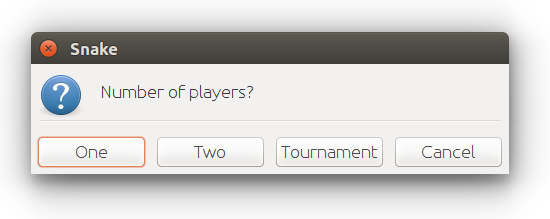
\includegraphics[width=1.0\textwidth]{../img/snake-start}

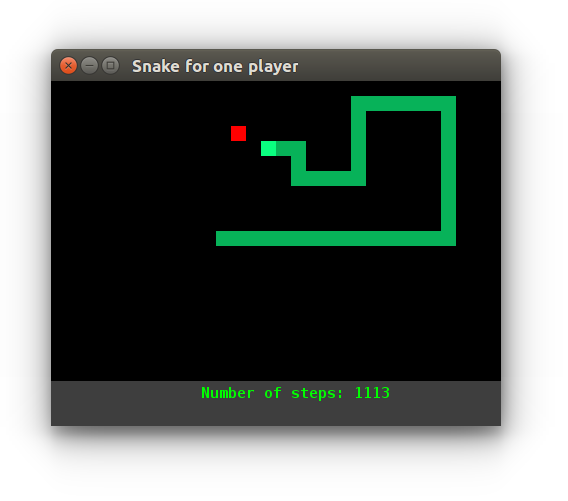
\includegraphics[width=1.0\textwidth]{../img/snake-oneplayer}
\end{minipage}
\begin{minipage}{0.5\textwidth}
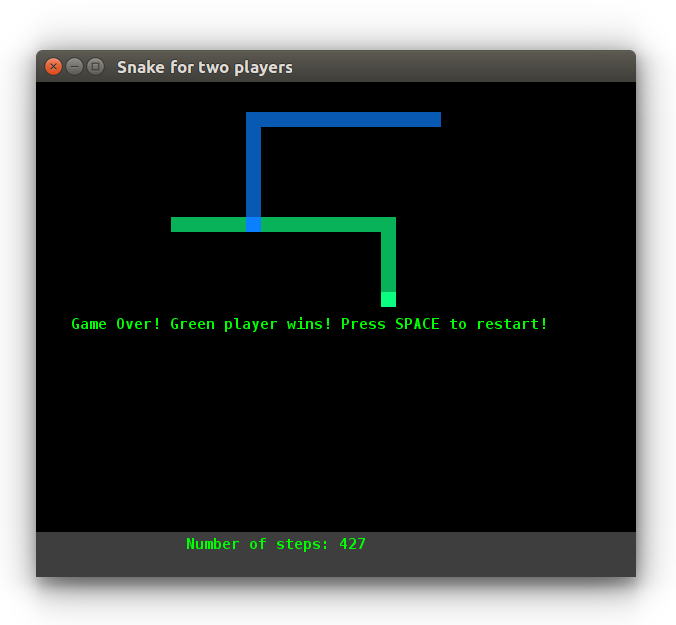
\includegraphics[width=1.0\textwidth]{../img/snake-twoplayer}
\end{minipage}
\caption{Spelet snake för en spelare med äpple och för två spelare utan äpple. \label{fig:snake-game}}
\end{figure}

\subsection{Obligatoriska funktionella krav}

Följande funktionella krav ska uppfyllas av ert program om ni är sex personer i gruppen. Om ni är färre ingår de obligatoriska krav som visas i tabell \ref{lab:snak:table-reqt}.
%\footnote{Om någon student, p.g.a. långvarig sjukdom eller annat giltigt skäl, genomför laborationen själv i efterhand som en individuell laboration ska följande krav implementeras på egen hand: \code{Player}, \code{OnePlayerGame}, \code{Snake}, \code{Apple}.}
\begin{itemize}[nosep, label={$\square$},]
\item \textbf{\texttt{Player}}. Det ska finnas spelare som motsvarar mänskliga användare och som har ett namn och fyra tangenter som den kan spela med. Varje spelare har en egen orm som den kan styra med sina tangenter.

\item \textbf{\texttt{Snake}}. Det ska finnas ormar. En orm består av ett antal block, där det främsta blocket kallas huvud och resten av blocken kallas svans. Huvudet har en ljusare färg än kroppen. Svansens längd ökar under spelets gång. En orm rör sig i en viss riktning och varje spelare kan ändra riktningen på sin orm med sina tangenter, i en av fyra riktningar \code{North}, \code{South}, \code{East} eller \code{West}.

\item \textbf{\texttt{Apple}}. Det ska finnas (minst ett) äpple. Ett äpple består av ett rött block och finns på en slumpvis position. Ett äpple kan ätas av en orm om ormens huvud träffar äpplet. Varje gång ett äpple äts upp av en orm så teleporteras äpplet till en ny position och kan ätas igen.

\item \textbf{\texttt{Banana}}. Det ska finnas (minst en) banan. En banan består av tre vertikala gula block och finns på en slumpvis position. En banan äts upp av en orm om ormens huvud träffar bananen. Varje gång en banan äts upp av en orm så teleporteras bananen till en ny slumpvis position och kan ätas igen.

\item \textbf{\texttt{Monster}}. Det ska finnas (minst ett) monster. Ett monster består av fem rosa block i kryssform.  Ett monster föds på en slumpvis position och rör sig i en riktning som bestäms vid monstrets födelse. Ett orm blir uppäten och dör om ormens huvud nuddar ett monsterblock .

\item \textbf{\texttt{OneplayerGame}}. Det ska gå att spela ensam. I varianten med en spelare finns en orm och minst ett äpple (och ev. även bananer och monster). Varje gång användarens orm lyckas äta en frukt får användaren poäng. När ormen ätit ett visst antal äpplen, eller om ormen blivit uppäten av ett monster, är spelet slut och poängen visas. En ormsvans ska bli längre vid jämna tidsintervall eller om den äter frukt.

\item \textbf{\texttt{TwoplayerGame}}. Det ska gå att spela två och två. I varianten med två spelare finns två ormar. Det finns också äpplen, bananer och monster. Om en orm äter en banan blir dess svans längre. När ormen ätit ett visst antal äpplen, eller om ormen blivit uppäten av ett monster, är spelet slut och poängen visas. En ormsvans ska bli längre vid jämna tidsintervall eller om den äter frukt.

\item \textbf{\texttt{Settings}}. Inställningar för spelet ska vara konfigurerbara genom en textfil som laddas i början av spelet. Inställningar ska vara en kontextparameter.  

\end{itemize}
\begin{table}[H]
  \centering
  \caption{Krav som minst ska implementeras vid respektive gruppstorlek. Om du har särskilda skäl kan du efter godkännande från kursansvarig göra labben enskilt.  \label{lab:snak:table-reqt}}

\begin{tabular}{r | c c c c c c}
  Krav / Antal personer & 1       & 2       & 3       & 4       & 5       & 6 \\ \hline
  \texttt{Player}       & $\surd$ & $\surd$ & $\surd$ & $\surd$ & $\surd$ & $\surd$ \\
  \texttt{OnePlayerGame}& $\surd$ &         &         &         & $\surd$ & $\surd$ \\
  \texttt{TwoPlayerGame}&         & $\surd$ & $\surd$ & $\surd$ & $\surd$ & $\surd$ \\
  \texttt{Snake}        & $\surd$ & $\surd$ & $\surd$ & $\surd$ & $\surd$ & $\surd$ \\
  \texttt{Apple}        & $\surd$ &         & $\surd$ & $\surd$ & $\surd$ & $\surd$ \\
  \texttt{Banana}       &         &         &         & $\surd$ &         & $\surd$ \\
  \texttt{Monster}      &         &         & $\surd$ &         &         & $\surd$ \\
  \texttt{Settings}     & $\surd$ & $\surd$ & $\surd$ & $\surd$ & $\surd$ & $\surd$ \\
\end{tabular}
\end{table}

\subsection{Obligatoriska design-krav}

\begin{enumerate}[label={$\square$}, leftmargin=*]

\item Snake-spel ska gå att starta med huvudprogrammet nedan. Huvudprogrammet får ändras vid behov i enlighet med minimikrav vad gäller gruppstorlek i tabell \ref{lab:snak:table-reqt}, samt valbara extrakrav i avsnitt \ref{lab:snake:extra-reqts}, och era egna ideer.
\scalainputlisting{../workspace/w10_snake/src/main/scala/snake/Main.scala}

\item Spelet ska bygga vidare på \code{introprog.BlockGame} enligt typhierarkin i fig.~\ref{snake:fig:game-hierarchy}.

\begin{figure}[H]
\begin{center}
\newcommand{\TextBox}[1]{\raisebox{0pt}[1em][0.5em]{#1}}
\tikzstyle{umlclass}=[rectangle, draw=black,  thick, anchor=north, text width=3cm, rectangle split, rectangle split parts = 3]
\begin{tikzpicture}[inner sep=0.5em,scale=1.0, every node/.style={transform shape}]

  \node [umlclass, rectangle split parts = 1, xshift=0cm, yshift=4.5cm] (BaseType)  {
              \textit{\textbf{\centerline{\TextBox{\code{BlockGame}}}}}
%              \nodepart[align=left]{second}\code{def x: T} \newline \code{def y: T}
          };


  \node [umlclass, rectangle split parts = 1, xshift=0cm, yshift=3.0cm] (SubType)  {
              \textit{\textbf{\centerline{\TextBox{\code{SnakeGame}}}}}
%              \nodepart[align=left]{second}\code{val x: Int} \newline \code{val y: Int}
          };

\node [umlclass, rectangle split parts = 1, xshift=-3cm, yshift=1.0cm] (SubSubType1)  {
            {\textbf{\centerline{\TextBox{\code{OnePlayerGame}}}}}
%            \nodepart[]{second}\TextBox{\code{val dim: Int}}
        };

\node [umlclass, rectangle split parts = 1, xshift=3cm, yshift=1.0cm] (SubSubType2)  {
            {\textbf{\centerline{\TextBox{\code{TwoPlayerGame}}}}}
%            \nodepart[]{second}\TextBox{\code{val dim: Int}}
        };

\draw[umlarrow] (SubType.north) -- ++(0,0.5) -| (BaseType.south);
\draw[umlarrow] (SubSubType1.north) -- ++(0,0.5) -| (SubType.south);
\draw[umlarrow] (SubSubType2.north) -- ++(0,0.5) -| (SubType.south);

\end{tikzpicture}
\end{center}
\caption{Arvshierarki med klassen \code{introprog.BlockGame} som bastyp.}
\label{snake:fig:game-hierarchy}
\end{figure}


\item Ormar, monster och frukt ska utgå från bastypen \code{Entity} enligt typhierarkin i ~\ref{snake:fig:entity-hierarchy}.

\begin{figure}[H]
\begin{center}
\newcommand{\TextBox}[1]{\raisebox{0pt}[1em][0.5em]{#1}}
\tikzstyle{umlclass}=[rectangle, draw=black,  thick, anchor=north, text width=2.5cm, rectangle split, rectangle split parts = 3]
\begin{tikzpicture}[inner sep=0.5em,scale=1.0, every node/.style={transform shape}]

  \node [umlclass, rectangle split parts = 1, xshift=0.0cm, yshift=4.5cm] (BaseType)  {
              \textit{\textbf{\centerline{\TextBox{\code{Entity}}}}}
%              \nodepart[align=left]{second}\code{def x: T} \newline \code{def y: T}
          };


  \node [umlclass, rectangle split parts = 1, xshift=-3.0cm, yshift=2.5cm] (SubType1)  {
              \textit{\textbf{\centerline{\TextBox{\code{CanMove}}}}}
%              \nodepart[align=left]{second}\code{val x: Int} \newline \code{val y: Int}
          };

\node [umlclass, rectangle split parts = 1, xshift=-4.75cm, yshift=0.5cm] (SubSubType01)  {
            {\textbf{\centerline{\TextBox{\code{Snake}}}}}
%            \nodepart[]{second}\TextBox{\code{val dim: Int}}
};

\node [umlclass, rectangle split parts = 1, xshift=-1.5cm, yshift=0.5cm] (SubSubType02)  {
            {\textbf{\centerline{\TextBox{\code{Monster}}}}}
%            \nodepart[]{second}\TextBox{\code{val dim: Int}}
};


\node [umlclass, rectangle split parts = 1, xshift=3.0cm, yshift=2.5cm] (SubType2)  {
            \textit{\textbf{\centerline{\TextBox{\code{CanTeleport}}}}}
%            \nodepart[]{second}\TextBox{\code{val dim: Int}}
        };

\node [umlclass, rectangle split parts = 1, xshift=1.75cm, yshift=0.5cm] (SubSubType1)  {
            {\textbf{\centerline{\TextBox{\code{Apple}}}}}
%            \nodepart[]{second}\TextBox{\code{val dim: Int}}
        };

\node [umlclass, rectangle split parts = 1, xshift=5.0cm, yshift=0.5cm] (SubSubType2)  {
            {\textbf{\centerline{\TextBox{\code{Banana}}}}}
%            \nodepart[]{second}\TextBox{\code{val dim: Int}}
        };


\draw[umlarrow] (SubType1.north) -- ++(0,0.5) -| (BaseType.south);
\draw[umlarrow] (SubType2.north) -- ++(0,0.5) -| (BaseType.south);
\draw[umlarrow] (SubSubType1.north) -- ++(0,0.5) -| (SubType2.south);
\draw[umlarrow] (SubSubType2.north) -- ++(0,0.5) -| (SubType2.south);
\draw[umlarrow] (SubSubType01.north) -- ++(0,0.5) -| (SubType1.south);
\draw[umlarrow] (SubSubType02.north) -- ++(0,0.5) -| (SubType1.south);

\end{tikzpicture}
\end{center}
\caption{Arvshierarki med klassen \code{Entity} som bastyp.}
\label{snake:fig:entity-hierarchy}
\end{figure}


\item \code{Entity} representerar en varelse i ett spel och ska se ut så här:
\scalainputlisting{../workspace/w10_snake/src/main/scala/snake/Entity.scala}
% \begin{Code}
% trait Entity {
%   def draw():   Unit
%   def erase():  Unit
%   def update(): Unit
%   def reset():  Unit
% }
% \end{Code}
Metoderna \code{draw} resp. \code{erase} anropas vid ritning resp. radering. Metoden \code{reset} återställer ursprungstillståndet. Metoden \code{update} anropas en gång i varje runda i spel-loopen. Predikatet \code{isOccupyingBlockAt} ger sant om positionen \code{p} finns bland de block som varelsen ockuperar på skärmen.

\item \code{CanMove} representerar en entitet som kan röra sig i en viss hastighet, enligt:
\scalainputlisting{../workspace/w10_snake/src/main/scala/snake/CanMove.scala}

% \begin{Code}
% trait MovingEntity extends Entity {
%   def move(): Unit
%
%   var movesPerSecond: Double = 20.0
%
%   final def millisBetweenMoves(): Int =
%     (1000 / movesPerSecond).round.toInt max 1
%
%   private var _timestampLastMove: Long = System.currentTimeMillis
%   final def timestampLastMove = _timestampLastMove
%
%   override final def update(): Unit =
%     if (System.currentTimeMillis > _
%           timestampLastMove + millisBetweenMoves) {
%       _timestampLastMove = System.currentTimeMillis
%       move()
%     }
% }
% \end{Code}

\item \code{CanTeleport} representerar en entitet som finns på en viss plats men som efter ett visst antal uppdateringar utan förvarning teleporterar sig till en ny position:
\scalainputlisting{../workspace/w10_snake/src/main/scala/snake/CanTeleport.scala}

\item Det ska finnas en enumeration \code{State} i singelobjektet \code{SnakeGame} som representerar spelets övergripande tillstånd enligt följande:
\begin{Code}
package snake 

object SnakeGame:
  enum State:
    case Starting, Playing, GameOver, Quitting
  export State.* // gör alla tillstånd synliga i SnakeGame
\end{Code}

\item Vid varje runda i spelloopen ska följande logik exekveras. Denna kod placeras förslagsvis i \code{gameLoopAction}, se vidare \code{SnakeGame} i avsnitt \ref{lab:snake:tips}.
\begin{Code}
    if state == Playing && !isPaused then
      _iterationsSinceStart += 1
      entities.foreach(_.erase())
      entities.foreach(_.update())
      entities.foreach(_.draw())
      onIteration()
      if isGameOver then enterGameOverState()
\end{Code}

\item Det ska finnas ett singelobjekt \code{Colors} där alla färger som används i spelet samlas.

\item Filen \code{pairs.scala} ska enligt laborationsförberedelser i övningsuppgift   \ref{exe:inheritance:labprep-pair} på sidan \pageref{exe:inheritance:labprep-pair} innehålla
\code{Pair[T]}, \code{Dim}, \code{Pos}, \code{Dir}, \code{North}, \code{South}, \code{East}, \code{West}. Se workspace här:\\
\url{https://github.com/lunduniversity/introprog/tree/master/workspace/}

\item Klassen \code{Player} ska se ut som följer:

\end{enumerate}

\scalainputlisting[basicstyle=\ttfamily\fontsize{10.5}{13}\selectfont]
{../workspace/w10_snake/src/main/scala/snake/Player.scala}




\subsection{Valbara krav -- varje person ska välja minst ett}\label{lab:snake:extra-reqts}

Varje person i gruppen ska implementera \emph{minst ett} (gärna flera) av kraven nedan. Vid implementation av flera av dessa krav blir spelet väsentligt roligare.
\begin{itemize}[nosep, label={$\square$}]

\item \textbf{\code{Points}}. Inför ett poängsystem, där poängen beror på t.ex. längden på svansen, antalet steg, antalet svängar, antal uppätna äpplen, etc.

\item \textbf{\code{Highscore}}. Spelet ska visa en lista med de spelare som fått flest poäng.

\item \texttt{\textbf{Äpple}}. Om inte redan ingår bland obl. krav enl.~ \ref{lab:snak:table-reqt}.

\item \textbf{\code{Monster}}. Om inte redan ingår bland obl. krav enl. 
\ref{lab:snak:table-reqt}.

\item \textbf{\code{Banan}}. Om inte redan ingår bland obl. krav enl. 
\ref{lab:snak:table-reqt}.

\item \textbf{\code{SelfTailCrash}}. Om en spelare kör in i sin egen orms svans så är spelet förlorat. (Om detta krav ej implementeras så \emph{får} man köra igenom sin egen svans utan att något händer.)

\item \textbf{\code{BoundaryCrash}}. Om en spelare kör utanför spelplanen så är spelet förlorat. (Om detta krav ej implementeras så ska ormen fortsätta på andra sidan spelplanen när man når kanten.)

\item \textbf{\code{EnterPlayerName}}. Spelare kan ange sitt namn, t.ex. via en dialog eller genom argument till \code{main}. Namnet används i meddelandefältet vid poängräkning och i meddelanden om vem som vunnit.

\item \textbf{\code{TwoPlayerComp extends Competition}}. Två spelare ska kunna tävla i en bäst-av-$n$-matcher-tävling i en sekvens av \code{TwoPlayerGame.play}, där den som vinner flest matcher blir blir totalvinnare.

\item \textbf{\code{SinglePlayerComp extends Competition}}. Flera spelare ska kunna tävla i en-persons-Snake, där den som får flest poäng av $n$ \code{OnePlayerGame}-spel blir totalvinnare.

\item \textbf{\code{Tournament extends Competition}}. Många spelare ska kunna spela en turnering.\footnote{\url{https://en.wikipedia.org/wiki/Tournament}} Namnen på spelarna läses in från en textfil. Valbara varianter:

\begin{itemize}[nosep, label={$\square$}]
\item \textbf{\code{KnockOut extends Tournament}}. Det ska gå att spela en utslagsturnering, som avslutas med final efter semi-final, etc., beroende på antal spelare.
\item \textbf{\code{RoundRobin extends Tournament}}. Det ska gå att spela en alla-möter-alla-turnering, där alla möjliga par av spelare möts i slumpvis ordning.
\end{itemize}

\end{itemize}


\subsection{Tips och förslag}\label{lab:snake:tips}

I detta stycke presenteras skisser till några av de klasser som behövs i enlighet med designkraven. Det är tillåtet att ändra, ta bort och lägga till, så länge de obligatoriska designkraven uppfylls. Koden finns här: \\
\url{https://github.com/lunduniversity/introprog/tree/master/workspace/}

% Här följer en skiss på klassen \code{Apple}:
% \scalainputlisting%[basicstyle=\ttfamily\fontsize{9.1}{12.2}\selectfont]
% {../workspace/w10_snake/src/main/scala/snake/Apple.scala}
% %
% Här följer en skiss på klassen \code{Banana}:
% \scalainputlisting%[basicstyle=\ttfamily\fontsize{9.1}{12.2}\selectfont]
% {../workspace/w10_snake/src/main/scala/snake/Banana.scala}
% Bananens ''kropp'' består av tre vertikalt ordnade blockpositioner i stället för en. Låt \code{pos}-attributet t.ex. betyda det översta av de tre bananblocken.

% Här följer en skiss på klassen \code{Banana}:
% \scalainputlisting%[basicstyle=\ttfamily\fontsize{9.1}{12.2}\selectfont]
% {../workspace/w10_snake/src/main/scala/snake/Monster.scala}
% Monsterkroppen består av fem blockpositioner ordnade som ett kryss. Låt \code{pos}-attributet t.ex. betyda det mittersta av de fem monsterblocken.


Här följer en skiss på klassen \code{Snake}:
\scalainputlisting[basicstyle=\ttfamily\fontsize{9}{12}\selectfont]
{../workspace/w10_snake/src/main/scala/snake/Snake.scala}


Här följer en skiss på den abstrakta klassen \code{SnakeGame} med de abstrakta metoderna \code{isGameOver} och \code{play} som överskuggas i de efterföljande underklasserna \code{OnePlayerGame} och \code{TwoPlayerGame}:
\scalainputlisting[basicstyle=\ttfamily\fontsize{9}{11.9}\selectfont]
{../workspace/w10_snake/src/main/scala/snake/SnakeGame.scala}


%!TEX encoding = UTF-8 Unicode

%!TEX root = ../compendium1.tex

%!TEX encoding = UTF-8 Unicode
\chapter{Scala och Java}\label{chapter:W11}
Koncept du ska lära dig denna vecka:
\begin{multicols}{2}\begin{itemize}[nosep,label={$\square$},leftmargin=*]
\item skillnader mellan Scala och Java
\item klasser i Scala vs Java
\item referensvariabler vs enkla värden i Java
\item referenstilldelning vs värdetilldelning i Java
\item alternativ konstruktor i Scala och Java
\item for-sats i Java
\item java for-each i Java
\item java.util.ArrayList
\item autoboxing i Java
\item primitiva typer i Java
\item wrapperklasser i Java
\item samlingar i Java vs Scala
\item scala.collection.JavaConverters
\item översiktligt om relationen mellan trait och interface
\item namnkonventioner för konstanter
\item enum i java ???\end{itemize}\end{multicols}


%%!TEX encoding = UTF-8 Unicode
\chapter{Scala och Java}\label{chapter:W11}
Koncept du ska lära dig denna vecka:
\begin{multicols}{2}\begin{itemize}[nosep,label={$\square$},leftmargin=*]
\item skillnader mellan Scala och Java
\item klasser i Scala vs Java
\item referensvariabler vs enkla värden i Java
\item referenstilldelning vs värdetilldelning i Java
\item alternativ konstruktor i Scala och Java
\item for-sats i Java
\item java for-each i Java
\item java.util.ArrayList
\item autoboxing i Java
\item primitiva typer i Java
\item wrapperklasser i Java
\item samlingar i Java vs Scala
\item scala.collection.JavaConverters
\item översiktligt om relationen mellan trait och interface
\item namnkonventioner för konstanter
\item enum i java ???\end{itemize}\end{multicols}


%!TEX encoding = UTF-8 Unicode
%!TEX root = ../exercises.tex

\ifPreSolution



\Exercise{\ExeWeekELEVEN}\label{exe:W11}

\begin{Goals}
\item Kunna förklara och beskriva viktiga skillnader mellan Scala och Java.
\item Kunna översätta enkla algoritmer, klasser och singeltonobjekt från Scala till Java och vice versa.
\item Känna till vad en case-klass innehåller i termer av en Javaklass.
%\item Förstå hur autoboxing fungerar.
\item Kunna använda Javatyperna \code{List}, \code{ArrayList}, \code{Set}, \code{HashSet} och översätta till deras Scalamotsvarigheter med \code{CollectionConverters}.
\item Kunna förklara hur autoboxning fungerar i Java, samt beskriva fördelar och fallgropar.
\end{Goals}

\begin{Preparations}
\item \StudyTheory{11}
\end{Preparations}

\BasicTasks %%%%%%%%%%%%%%%%

\else



\ExerciseSolution{\ExeWeekELEVEN}

\BasicTasks %%%%%%%%%%%

\fi





\WHAT{Översätta metoder från Java till Scala.}

\QUESTBEGIN

\Task  \what~  I denna uppgift ska du översätta en Java-klass som används som en modul\footnote{\href{https://en.wikipedia.org/wiki/Modular_programming}{en.wikipedia.org/wiki/Modular\_programming}} och bara innehåller statiska metoder och inget förändringsbart tillstånd som kan ändras utifrån. (I nästa uppgift ska du sedan översätta klasser med förändringsbara  tillstånd.)

Vi börjar med att göra översättningen från Java till Scala rad för rad och du ska behålla så mycket som möjligt av syntax och semantik så att Scala-koden blir så Java-lik som möjligt. I efterföljande deluppgift ska du sedan omforma översättningen så att Scala-koden blir mer idiomatisk\footnote{\href{https://sv.wikipedia.org/wiki/Idiom_\%28programmering\%29}{sv.wikipedia.org/wiki/Idiom\_\%28programmering\%29}}.

\Subtask Studera klassen \code{Hangman} nedan. Du ska översätta den från Java till Scala enlig de riktlinjer och tips som följer efter koden. Läs igenom alla riktlinjer och tips innan du börjar.

\javainputlisting[numbers=left]{examples/scalajava/Hangman.java}

\noindent\emph{Riktlinjer och tips för översättningen:}

\begin{enumerate}[noitemsep]

\item Skriv Scala-koden med en texteditor i en fil som heter \texttt{hangman1.scala} och kompilera med \code{scalac hangman1.scala} i terminalen; använd alltså \emph{inte} en IDE, så som Eclipse eller IntelliJ, utan en ''vanlig'' texteditor, t.ex. VS \code{code}.

\item Översätt i denna första deluppgift rad för rad så likt den ursprungliga Java-kodens utseende (syntax)  som möjligt, med så få ändringar som möjligt. Du ska alltså ha kvar dessa Scalaovanligheter, även om det inte alls blir som man brukar skriva i Scala:
\begin{enumerate}[nolistsep, noitemsep]
\item långa indrag, \item onödiga semikolon, \item onödiga \code{()}, \item onödiga \code|{}|, \item onödiga \code{System.out}, och \item onödiga \code{return}.
\end{enumerate}

\item Försök också i denna deluppgift göra så att betydelsen (semantiken) så långt som möjligt motsvarar den i Java, t.ex. genom att använda \code{var} överallt, även där man i Scala normalt använder \code{val}.

\item En Javaklass med bara statiska medlemmar motsvarar ett singeltonobjekt i Scala, alltså en \code{object}-deklaration innehållande ''vanliga'' medlemmar.

\item För att tydliggöra att du använder Javas \code{Set} och \code{HashSet} i din Scala-kod, använd följande import-satser i \code{hangman1.scala}, som därmed döper om dina importerade namn och gör så att de inte krockar med Scalas inbyggda \code{Set}. Denna form av import går inte att göra i Java.
\begin{Code}
import java.util.{Set => JSet};
import java.util.{HashSet => JHashSet};
\end{Code}

\item Javas \code{i++} fungerar inte i Scala; man får istället skriva \code{i += 1} eller mindre vanliga \code{i = i + 1}.

\item Typparametrar i Java skrivs inom \code{<>} medan Scalas syntax för typparametrar använder \code{[]}.

\item Till skillnad från Java så har Scalas metoddeklarationer ett tilldelningstecken \code{=} efter returtypen, före kroppen.

\item Du kan ladda ner Java-koden till \code{Hangman}-klassen nedan från kursens repo%
\footnote{\href{https://github.com/lunduniversity/introprog/blob/master/compendium/examples/scalajava/Hangman.java}{github.com/lunduniversity/introprog/blob/master/compendium/examples/scalajava/Hangman.java}}. I samma bibliotek ligger även lösningarna till översättningen i Scala, men kolla \emph{inte} på dessa förrän du gjort klart översättningarna och fått dem att kompilera och köra felfritt! Tanken är att du ska träna på att läsa felmeddelande från kompilatorn och åtgärda dem i en upprepad kompilera-testa-rätta-cykel.

\end{enumerate}







\Subtask Skapa en ny fil \code{hangman2.scala} som till att börja med innehåller en kopia av din direkt-översatta Java-kod från föregående deluppgift. Omforma koden så att den blir mer som man brukar skriva i Scala, alltså mer Scala-idiomatisk. Försök förenkla och förkorta så mycket du kan utan att göra avkall på läsbarheten.

\emph{Tips och riktlinjer:}

\begin{enumerate}[nolistsep, noitemsep]

\item Kalla Scala-objektet för \code{hangman}. När man använder ett Scalaobjekt som en modul (alltså en samling funktioner i en gemensam, avgränsad namnrymd) har man gärna liten begynnelsebokstav, i likhet med konventionen för paketnamn. Ett paket är ju också en slags modul och med en namngivningskonvention som är gemensam kan man senare, utan att behöva ändra koden som använder modulen, ändra från ett singelobjekt till ett paket och vice versa om man så önskar.

\item Gör alla metoder publikt tillgängliga och låt även strängvektorn \code{hangman} vara publikt tillgänglig. Deklarera \code{hangman} som en \code{val} och konstruera den med \code{Vector}. Eftersom \code{Vector} är oföränderlig och man inte kan ärva från singelobjekt och \code{hangman} är deklarerad med \code{val} finns inga speciella risker med att göra den konstanta vektorn publik om  vi inte har något emot att annan kod kan läsa (och eventuellt göra sig beroende av) vår hänggubbetext.

\item I metoden \code{renderHangman}, använd \code{take} och \code{mkString}.

\item I metoden \code{hideSecret}, använd \code{map} i stället för en \code{for}-sats.

\item Det går att ersätta metoden \code{foundAll} med det kärnfulla uttrycket \\ \code{(secret forall found)} där \code{secret} är en sträng och \code{found} är en mängd av tecken (undersök gärna i REPL hur detta fungerar). Skippa därför den metoden helt och använd det kortare uttrycket direkt.

\item I metoden \code{makeGuess}, i stället för \code{Scanner}, använd \code{scala.io.StdIn.readLine}.

\item Om du vill träna på att använda rekursion i stället för imperativa loopar: Gör metoden \code{makeGuess} rekursiv i stället för att använda \code{do}-\code{while}.

\item I metoden \code{download}, i stället för \code{java.net.URL} och \code{java.util.ArrayList}, använd \code{scala.io.Source.fromURL(address, coding).getLines.toVector} och gör en lokal import av \code{scala.io.Source.fromURL} överst i det block där den används. Det går inte att ha lokala \code{import}-satser i Java.

\item Låt metoden \code{download} returnera en \code{Option[String]} som i fallet att nedladdningen misslyckas returnerar \code{None}.

\item I metoden \code{download}, i stället för \code{try}-\code{catch} använd \code{scala.util.Try} och dess smidiga metod \code{toOption}.

\item Om du vill träna på att använda rekursion i stället för imperativa loopar: Använd, i stället för \code{while}-satsen i metoden \code{play}, en lokal rekursiv funktion med denna signatur:
\begin{Code}
  def loop(found: Set[Char], bad: Int): (Int, Boolean)
\end{Code}
Funktionen \code{loop} returnerar en 2-tupel med antalet felgissningar och \code{true} om man hittat alla bokstäver eller \code{false} om man blev hängd.

\end{enumerate}





\SOLUTION


\TaskSolved \what
     %%%TODO number  1 %%%starts with: \emph{Översätta algoritmer och %%%

\SubtaskSolved  \scalainputlisting[numbers=left,basicstyle=\ttfamily\fontsize{10.3}{12}\selectfont]{examples/scalajava/hangman1.scala}

\SubtaskSolved  \scalainputlisting[numbers=left,basicstyle=\ttfamily\fontsize{11.2}{13}\selectfont]{examples/scalajava/hangman2.scala}



\QUESTEND






\WHAT{Översätta mellan klasser i Scala och klasser i Java.}

\QUESTBEGIN

\Task  \what~
Klassen \code{Point} nedan är en modell av en punkt som kan sparas på begäran i en lista. Listan är privat för kompanjonsobjektet och kan skrivas ut med en metod \code{showSaved}. I koden används en \code{ArrayBuffer}, men i framtiden vill man, vid behov, kunna ändra från \code{ArrayBuffer} till en annan sekvenssamlingsimplementation, t.ex. \code{ListBuffer}, som uppfyller egenskaperna hos supertypen \code{Buffer}, men har andra prestandaegenskaper för olika operationer. Därför är attributet \code{saved} i kompanjonsobjektet deklarerat med den mer generella typen.

\scalainputlisting[numbers=left]{examples/scalajava/Point.scala}

\Subtask Översätt klassen \code{Point} ovan från Scala till Java. Vi ska i nästa deluppgift kompilera både Scala-programmet ovan och ditt motsvarande Java-program i terminalen och testa i REPL att klasserna har motsvarande funktionalitet.

\emph{Tips och riktlinjer:}
\begin{enumerate}[nolistsep, noitemsep]
\item För att namnen inte ska krocka i våra kommande tester, kalla Javatypen för \code{JPoint}.
\item  I stället för Scalas \code{ArrayBuffer} och \code{Buffer}, använd Javas \code{ArrayList} och \code{List} som båda ligger i paketet \code{java.util}.
\item Undersök dokumentationen för \code{java.util.List} för att hitta en motsvarighet till \code{prepend} för att lägga till i början av listan.
\item I stället för default-argumentet i Scalas primärkonstruktor, använd en extra Java-konstruktor.
\item Det finns inga singelobjekt och inga kompanjonsobjekt i Java; istället kan man använda statiska klassmedlemmar. Placera kompanjonsobjektets medlemmars motsvarigheter \emph{inuti} Java-klassen och gör dem till \jcode{static}-medlemmar.
\item Kod i klasskroppen i Scalaklassen, så som if-satsen på rad 4, placeras i lämplig konstruktor i Javaklassen.
\item Utskrifter med \code{print} och \code{println} behöver i Java föregås av \code{System.out}.
\item Det finns inget nyckelord \code{override} i Java, men en s.k. annotering som ger samma kompilatorhjälp. Den skrivs med ett snabel-a och stor begynnelsebokstav, så här: \jcode{ @Override }  före metoddeklarationen.
\item I Java används konventionen att börja getter-metoder med ordet \code{get}, t.ex. \code{getX()}.
\item Det finns ingen motsvarighet till \code{mkString} för \code{List} så du behöver själv gå igenom listan och hämta elementreferenser för utskrift med en \jcode{for}-loop. Notera att efter sista elementet ska radbrytning göras i utskriften och att inget komma ska skrivas ut efter sista elementet.
\item I Java behövs en ny \jcode{import}-deklaration om man vill importera ännu en typ från samma paket. Man kan även i Java använda asterisk \code{*}, (motsvarande \code{_} i Scala), för att importera allt i ett paket, men då får man med alla möjliga namn och det vill man kanske inte.
\item Metoder i Java slutar med \code{()} om de saknar parametrar.
\item Alla satser i Java slutar med lättglömda semikolon. (Efter att man i skrivit mycket Javakod och växlar till Scalakod är det svårt att vänja sig av med att skriva semikolon...)
\end{enumerate}


\Subtask Starta REPL i samma bibliotek som du kompilerat kodfilerna. Testa så att klasserna \code{Point} och \code{JPoint} beter sig på samma vis enligt nedan. Skriv även testkod i REPL för att avläsa de attributvärden som har getters och undersök att allt funkar som det ska.
\begin{REPLnonum}
$ scalac Point.scala
$ javac JPoint.java
$ scala
scala> val (p, jp) = (new Point, new JPoint)
scala> p.distanceTo(new Point(3, 4))
scala> Point.showSaved
scala> jp.distanceTo(new JPoint(3, 4))
scala> JPoint.showSaved
scala> for (i <- 1 to 10) { new Point(i, i, true) }
scala> Point.showSaved
scala> for (i <- 1 to 10) { new JPoint(i, i, true) }
scala> JPoint.showSaved
\end{REPLnonum}


\Subtask Översätt nedan Javaklass \code{JPerson} till en \code{case class Person} i Scala med  motsvarande funktionalitet.


\javainputlisting[numbers=left]{examples/scalajava/JPerson.java}


\Subtask\Pen Undersök i REPL vilken funktionalitet i Scala-case-klassen \code{Person} som \emph{inte} är implementerad i Java-klassen \code{JPerson} ovan. Skriv upp namnen på några av case-klassens extra metoder samt deras signatur genom att för en \code{Person}-instans, och för kompanjonsobjektet \code{Person}, trycka på TAB-tangenten. Prova några av de extra metoderna i REPL och förklara vad de gör.

\begin{REPL}
scala> val p = Person("Björn", 49)
scala> p.      // tryck TAB en gång
scala> Person. // tryck TAB en gång
scala> p.copy  // tryck TAB en gång
scala> p.copy()
scala> p.copy(age = p.age + 1)
scala> Person.unapply(p)
\end{REPL}


\SOLUTION


\TaskSolved \what
     %%%TODO number  2 %%%starts with: \emph{Översätta mellan klasser %%%

\SubtaskSolved   \javainputlisting[numbers=left]{examples/scalajava/JPoint.java}

\SubtaskSolved   -

\SubtaskSolved   \begin{Code}
case class Person(name: String, age: Int = 0)
\end{Code}

\SubtaskSolved  p.*TAB* - copy, producArity, ProductIterator, productElement, productPrefix

Person.*TAB* - apply, curried, tupled, unapply

\begin{REPLnonum}
scala> p.copy
   def copy(name: String,age: Int): Person

scala> p.copy()
res0: Person = Person(Björn,49)

scala> p.copy(age = p.age + 1)
res1: Person = Person(Björn,50)

scala> Person.unapply(p)
res2: Option[(String, Int)] = Some((Björn,49))
\end{REPLnonum}



\QUESTEND






\WHAT{Auto(un)boxing.}

\QUESTBEGIN

\Task  \what~  I JVM måste typparametern för generiska klasser vara av referenstyp. I Scala löser kompilatorn detta åt oss så att vi ändå kan ha t.ex. \code{Int} som argument till en typparameter i Scala, medan man i Java \emph{inte} direkt kan ha den primitiva typen \jcode{int} som typparameter till t.ex. \code{ArrayList}.

I Java och i den underliggande plattformen JVM används s.k. wrapper-klasser för att lösa detta, t.ex. genom wrapper-klassen \code{Integer} som boxar den primitiva typen \jcode{int}. Java-kompilatorn har stöd för att automatiskt packa in värden av primitiv typ i sådana wrapper-klasser för att skapa referenstyper och kan även automatiskt packa upp dem.

\Subtask Studera hur Scala-kompilatorn låter oss arbeta med en \code{Cell[Int]} även om det underliggande JVM:ens körtidstyp \Eng{runtime type} är en wrapper-klass. Man kan se JVM-körtidstypen med metoderna \code{getClass} och \code{getTypeName} enligt nedan.
\begin{REPL}
scala> class Cell[T](var value: T){
         val typeName: String = value.getClass.getTypeName
         override def toString = "Cell[" + typeName + "](" + value + ")"
       }
scala> val c = new Cell[Int](42)
scala> c.value.getClass.getTypeName
\end{REPL}


\Subtask Vad är körtidstypen för \code{c.value} ovan? Förklara hur det kan komma sig trots att vi deklarerade med typargumentet \code{Int}?

\Subtask Studera dokumentationen för \code{java.lang.Integer}\footnote{\href{https://docs.oracle.com/javase/8/docs/api/java/lang/Integer.html}{docs.oracle.com/javase/8/docs/api/java/lang/Integer.html}} och testa i REPL några av \emph{klassmetoderna} (de som är \jcode{static} och därmed kan anropas med punktnotation direkt på klassens namn utan \code{new}) och några av \emph{instansmetoderna} (de som inte är \jcode{static}).
\begin{REPL}
scala> Integer.  //tryck TAB
scala> Integer.
scala> Integer.toBinaryString(42)
scala> Integer.valueOf(42)
scala> val i = new Integer(42)
scala> i.  // tryck TAB
scala> i.toString
scala> i.compareTo  // tryck TAB 2 gånger
scala> i.compareTo(Integer.valueOf(42))
scala> i.compareTo(42)  // varför fungerar detta?
\end{REPL}

\Subtask\Pen Enligt dokumentationen\footnote{\href{https://docs.oracle.com/javase/8/docs/api/java/lang/Integer.html\#compareTo-java.lang.Integer-}{docs.oracle.com/javase/8/docs/api/java/lang/Integer.html\#compareTo-java.lang.Integer-}} tar instansmetoden \code{compareTo} i klassen \code{Integer} en \code{Integer} som parameter. Hur kan det då komma sig att sista raden ovan fungerar med en \code{Int}?

\Subtask Studera nedan Java-program och beskriv vad som kommer att skrivas ut \emph{innan} du kompilerar och testkör.

\javainputlisting[numbers=left]{examples/scalajava/Autoboxing.java}

\Subtask Ändra i programmet ovan så att autoboxing och autounboxing utnyttjas på alla ställen där så är möjligt. Utnyttja även att \code{toString}-metoden på \code{Integer} ger samma stränrepresentation som \jcode{int} vid utskrift. Fixa också så att du undviker \emph{fallgropen} att i Java jämföra med referenslikhet i stället för att använda \code{equals}. Testa så att allt fungerar som det borde efter dina ändringar.


\Subtask\Pen Antag att du råkar skriva \jcode{xs.add(0, pos)} på rad 14 i ditt program från föregående uppgift. Förklara hur autoboxingen stjälper dig i en \emph{fallgrop} då.

\Subtask\Pen Med ledning av de båda tidigare deluppgifterna: sammanfatta de två nämnda fallgropar med autoboxing i Java i två generella punkter, så att du har nytta av att memorera dem inför din framtida Javakodning.


\SOLUTION


\TaskSolved \what
     %%%TODO number  3 %%%starts with: \emph{Auto(un)boxing.} I JVM må%%%

\SubtaskSolved   -

\SubtaskSolved   Cell har typen java.lang.Integer. När man hämtar ut värdet med \code{c.value} hämtas den primitiva typ \code{int} ut.

\SubtaskSolved   Med hjälp av autoboxing förvandlas 42 till typen \code{Integer} och kan därför jämföras med en annan \code{Integer}.

\SubtaskSolved   i.compareTo(42) fungerar på grund av autoboxing. Då JVM packar in den primitiva typ int i en Integer-objekt automatiskt.

\SubtaskSolved
\begin{REPLnonum}
0 10 20 30 40 50 60 ... 390 400 410

[0]: 0
[42]: 0
NOT EQUAL
\end{REPLnonum}

\SubtaskSolved   \javainputlisting[numbers=left]{examples/scalajava/Autoboxing2.java}

\SubtaskSolved   42 kommer läggas längst fram i listan istället för längst bak, då autounboxing kommer göra Integer(0) till 0 och tvärtom med variablen \code{pos}.

\SubtaskSolved   Om man ska undersöka om två int-variabler är lika ska man använda ==, men om variablerna är av typen Integer måste man använda \code{equals}.

JVM kommer inte varna om man vänder på \code{Integer} och \code{int}, som i \code{xs.add(0, pos)}.



\QUESTEND






\WHAT{JavaConverters.}

\QUESTBEGIN

\Task  \what~  Med \code{import scala.jdk.CollectionConverters._} får man i sina Scalaprogram tillgång till de smidiga metoderna \code{asJava} och \code{asScala} som översätter mellan motsvarande samlingar i resp språks standardbibliotek. Kör nedan i REPL och gör efterföljande deluppgifter.

\begin{REPL}
scala> val sv = Vector(1,2,3)
scala> val ss = Set('a','b','c')
scala> val sm = Map("gurka" -> 42, "tomat" -> 0)
scala> val ja = new java.util.ArrayList[Int]
scala> ja.add(42)
scala> val js = new java.util.HashSet[Char]
scala> js.add('a')
scala> import scala.jdk.CollectionConverters._
\end{REPL}

\Subtask Till vilka typer konverteras Scalasamlingarna
\code{Vector[Int]}, \code{Set[Char]} och \\ \code{Map[String, Int]} om du anropar metoden \code{asJava} på dessa?

\Subtask Till vilka typer konverteras Javasamlingarna \code{ArrayList[Int]} och \code{HashSet[Char]}  om du anropar metoden \code{asScala} på dessa? Blir det föränderliga eller oföränderliga motsvarigheter?

\Subtask Vad får resultatet för typ om du kör \code{toSet} på en samling av typen \code{mutable.Set}?

\Subtask Undersök hur du kan efter att du gjort \code{sm.asJava.asScala} anropa ytterligare en metod för att få tillbaka en oföränderlig \code{immutable.Map}.

\Subtask Läs mer i dokumentationen om JavaConverters\footnote{\href{http://docs.scala-lang.org/overviews/collections/conversions-between-java-and-scala-collections.html}{docs.scala-lang.org/overviews/collections/conversions-between-java-and-scala-collections.html}}
och prova några fler konverteringar.



\SOLUTION


\TaskSolved \what
     %%%TODO number  4 %%%starts with: \emph{JavaConverters.} Med \cod%%%

\SubtaskSolved

Vector[Int] -> java.util.List[Int]

Set[Char] -> java.util.Set[Char]

Map[String, Int] -> java.util.Map[String, Int]

\SubtaskSolved

ArrayList[Int] -> scala.collection.mutable.Buffer[Int]

HashSet[Char] -> scala.collection.mutable.Set[Char]

Båda blir föränderliga motsvarigheter. Det visas genom att de till hör \code{scaka.collection.mutable} och både \code{ArrayList} och \code{HashSet} är förändrliga i Java.

\SubtaskSolved   \code{scala.collection.immutable.Set}

\SubtaskSolved   \code{sm.asJava.asScala} ger typen \code{scala.collection.mutable.Map[String,Int]}

\code{sm.asJava.asScala.toMap} ger typen \code{scala.collection.immutable.Map[String,Int]}

\SubtaskSolved   -

\QUESTEND




\ExtraTasks %%%%%%%%%%%%%%%%%%%


\WHAT{Översätta från Java till Scala.}

\QUESTBEGIN

\Task  \what~ Översätt nedan kod från Java till Scala. Skriv koden i en fil som heter \texttt{showInt.scala} och kalla Scala-objektet med \code{main}-metoden för \code{showInt}. Läs tipsen som följer efter koden innan du börjar.

\javainputlisting[numbers=left]{examples/scalajava/JShowInt.java}

\emph{Tips:}
\begin{itemize}[nolistsep, noitemsep]
\item En Javaklass med bara statiska medlemmar motsvaras av ett singeltonobjekt i Scala, alltså en \code{object}-deklaration. Scala har därför inte nyckelordet \jcode{static}.
\item Typen \jcode{Object} i Java motsvaras av Scalas \code{Any}.
\item Du kan använda Scalas möjlighet med default-argument (som saknas i Java) för att bara definiera en enda \code{show}-metod med en tom sträng som default \code{msg}-argument.
\item I Scala har objekt av typen \code{Char} en metod \code{def *(n: Int): String} som skapar en sträng med tecknet repeterat \code{n} gånger. Men du kan ju välja att ändå implementera metoden \code{repeatChar} med \code{StringBuilder} som nedan om du vill träna på att översätta en \code{for}-loop från Java till Scala.
\item I stället för \code{Scanner.nextLine} kan du använda \code{scala.io.StdIn.readLine} som tar en prompt som parameter, men du kan också använda \code{Scanner} i Scala om du vill träna på det.
\item I Java \emph{måste} man använda nyckelordet \jcode{return} om metoden inte är en \jcode{void}-metod, medan man i Scala faktiskt \emph{får} använda \code{return} även om man brukar undvika det och i stället utnyttja att satser i Scala också är uttryck.
\end{itemize}
Kompilera din Scala-kod och kör i terminalen och testa så att allt funkar. Vill du även kompilera Java-koden så finns den i kursens repo i filen\\ \texttt{compendium/examples/scalajava/JShowInt.java}


\SOLUTION


\TaskSolved \what


\begin{Code}[numbers=left]
object showInt {
  def show(obj: Any, msg: String = ""): Unit = println(msg + obj)

  def repeatChar(ch: Char, n: Int): String = ch.toString * n

  def showInt(i: Int): Unit = {
    val leading = Integer.numberOfLeadingZeros(i)
    val binaryString = repeatChar('0', leading) + i.toBinaryString
    show(i,               "Heltal : ")
    show(i.asInstanceOf[Char],         "Tecken : ")
    show(binaryString,    "Binärt : ")
    show(i.toHexString,   "Hex    : ")
    show(i.toOctalString, "Oktal  : ")
  }


  import scala.io.StdIn.readLine
  import scala.util.{Try,Success,Failure}

  def loop: Unit =
    Try { readLine("Heltal annars pang: ").toInt } match {
      case Failure(e) => show(e); show("PANG!")
      case Success(i) => showInt(i); loop
    }

  def main(args: Array[String]): Unit =
    if(args.length > 0) args.foreach(i => showInt(i.toInt))
    else loop
}
\end{Code}



\QUESTEND






\WHAT{Innehållslikhet och referenslikhet i Java.}

\QUESTBEGIN

\Task  \what~ Studera och prova denna fallgrop med innehållslikhet: \href{https://github.com/bjornregnell/lth-eda016-2015/blob/master/lectures/examples/eclipse-ws/lecture-examples/src/week10/generics/TestPitfall3.java}{TestPitfall3.java}







\SOLUTION


\TaskSolved \what
     %%%TODO number  6 %%%starts with: \TODO Fallgrop med Point som in%%%



\QUESTEND




\AdvancedTasks %%%%%%%%%%%%%%%%%


\WHAT{Implementera innehållslikhet i Java.}

\QUESTBEGIN

\Task  \what~\Pen Studera fallgropar för hur man skriver en \code{equals}-metod i Java här:
\href{http://www.artima.com/lejava/articles/equality.html}{www.artima.com/lejava/articles/equality.html} och jämför med  det fullständiga receptet för hur man skriver en välfungerande \code{equals} och \code{hashcode} i Scala här: \href{http://www.artima.com/pins1ed/object-equality.html}{www.artima.com/pins1ed/object-equality.html}

\Subtask Vilka skillnader och likheter finns vid överskuggning av equals i Java respektive Scala, som ska ge en fungerande innehållstest för en hierarki med bastyper och subtyper?

\Subtask Vilka fallgropar är gemensamma för Java och Scala?\SOLUTION


\TaskSolved \what
     %%%TODO number  7 %%%starts with: \TODO \emph{Gränssnitt i Scala %%%



\QUESTEND

%!TEX encoding = UTF-8 Unicode
%!TEX root = ../compendium2.tex

\Lab{\LabWeekELEVEN}

\begin{Goals}
\item Förstå skillnaden mellan primitiva typer och objekt i Java.
\item Kunna förklara hur autoboxing fungerar i Java.
\item Kunna förklara vad statiska metoder och attribut i Java innebär.
\item Kunna använda \code{ArrayList} och arrayer i Java.
\item Kunna använda Java-klassen \code{Scanner}.
\item Kunna skapa en for-sats i Java.
\item Känna till hur man kan förenkla användandet av Java och Scala i samma program med hjälp av \code{scala.collection.JavaConverters}.
\end{Goals}

\begin{Preparations}
\item \DoExercise{\ExeWeekELEVEN}{11}
\item Studera given kod här: \url{https://github.com/lunduniversity/introprog/tree/master/workspace/w11_javatext/}
\end{Preparations}

\subsection{Krav}

Du ska skapa ett textspel för terminalen som är (lagom) intressant/roligt att spela, sparar poäng per spelomgång för olika spelare och mäter tiden det tog att spela. Till din hjälp har du den färdiga filen \code{Main.java} (som går bra att förändra om det behövs) samt de två kodskeletten \code{Game.java} och \code{UserInterface.scala}. Ditt textspel ska köras i terminalen och uppfylla följande krav och riktlinjer:

\begin{enumerate}
  \item När ditt program kör ska man ska kunna starta flera spelomgångar efter varandra utan att behöva avsluta programmet.
  \item För varje spelomgång ska programmet komma ihåg spelarens namn\footnote{eller spelar\emph{nas} namn om det är ett spel för två eller flera personer} med tillhörande resultat.
  \item Efter begäran ska programmet kunna visa en topplista med bästa poäng, både för alla spelare och för ett specifikt spelarnamn.
%  \item Speltiden för varje spelomgång ska mätas och sparas tillsammans med poängresultatet för respektive spelare.
  \item Koden för själva spelet ska vara skriven i Java, men Scala ska användas för att implementera funktionerna i singelobjektet \code{UserInterface}.
  \item I Scala-koden ska du för träningens skull använda Java-klassen \code{java.util.Scanner} när du läser in data från terminalen.
  \item Koden i singelobjektet \code{UserInterface} ska använda omvandlingsmetoden \code{asScala} efter \code{import scala.collection.JavaConverters._} för att omvandla argument av typen \code{java.util.ArrayList}.
  \item Ditt spel ska i Java-kod använda minst en av datastrukturerna
  \code{ArrayList},
  \code{HashSet},
  \code{HashMap} ur paketet \code{java.util}, samt minst en array. (Den givna koden i \code{Main.java} räknas inte till detta krav.)
  \item Du ska spela någon annans halvfärdiga spel och, efter att du studerat koden, ge återkoppling på kodens läsbarhet.
  \item Du ska låta någon annan spela ditt halvfärdiga spel och visa din kod och fråga om återkoppling på läsbarheten. Du ska anteckna den återkoppling du får.
  \item Du ska inför redovisningen förbereda följande:
  \begin{enumerate}
    \item en kort genomgång av spelets idé,
    \item en kort förklaring av kodens struktur och de olika Java-klassernas ansvar,
    \item en kort redogörelse för den återkoppling du fått på din kods läsbarhet och hur du arbetat med att förbättra läsbarheten under dina stegvisa utvidgningar av din kod,
    \item en lista med koncept som du tränat på när du skapat ditt textspel.
  \end{enumerate}
\end{enumerate}

\subsection{Frivilliga extrauppgifter}

\begin{enumerate}
	\item Spara resultat i en fil efter varje spelomgång, och läs in resultat från filen antingen när programmet startas eller när användaren vill se poänglistan, så att det går att se spelresultat från tidigare körningar av programmet. Den kod du behöver lägga till för att åstadkomma detta kan vara skriven antingen i Java eller Scala. Tänk på att du kan behöva göra ändringar även i \code{Main}-klassen.
	\item   Mät speltiden för varje spelomgång och spara tiden tillsammans med poängresultatet för respektive spelare.

\end{enumerate}

\subsection{Inspiration och tips}

\begin{enumerate}
  \item Utgå från Hangman i veckans övning eller,
  \item Yatzy från tidigare övningar, eller
  \item skapa ett kortspel inspirerat av \code{shuffle}-labben, eller
  \item inspireras av listan med sällskapsspel på wikipedia:\\ \href{https://sv.wikipedia.org/wiki/Kategori:Sällskapsspel}{sv.wikipedia.org/wiki/Kategori:Sällskapsspel}
  \item eller hitta på ett eget textspel.
  \item Börja med en starkt förenklad variant som du sedan bygger vidare på.
  \item Kompilera och testa efter varje ändring, så att du hela tiden har ett fungerande program.
  \item Dela upp din spelkod i flera metoder, och även flera klasser om det är lämpligt.
  \item Det finns mycket information på nätet om hur man skriver Java-kod och använder JDK, t.ex. på \url{https://stackoverflow.com/}
  \item Träna på att använda JDK-dokumentationen här:\\ \url{https://docs.oracle.com/javase/8/docs/api/}
\end{enumerate}


%!TEX encoding = UTF-8 Unicode

%!TEX root = ../compendium1.tex

\chapter{Trådar, Web, Android}
\begin{itemize}[nosep]
\item Thread
\item Future
\item HTML
\item Javascript
\item css
\item Scala.js
\item Android
\end{itemize}
\clearpage
%!TEX encoding = UTF-8 Unicode
%!TEX root = ../lect-week11.tex

%%%

\ifkompendium\else

\Subsection{Veckans labb: \texttt{survey2}}
\begin{Slide}{Veckans labb: \texttt{survey2}}\SlideFontTiny
\begin{minipage}{0.65\textwidth}
Nya version 2 av labben är enklare och kräver ej att du implementerar parsning av \code{args}. Välj själv vilken du gör.

\vspace{0.5em}
\Emph{Förberedelse:}
\begin{itemize}
\item Studera givna koden: {\SlideFontTiny \href{https://github.com/lunduniversity/introprog/tree/master/workspace/w10_survey2/src/main/scala/stats}{workspace/w10\_survey2}}
\item Fyll i denna enkät:
\\{\SlideFontTiny \url{https://goo.gl/forms/hC6JK2UQXVpbGECc2}} 
\end{itemize}

\Emph{Grunduppgift:}
\begin{itemize}
\item Implementera en klass \code{Table} för hantering av strängmatriser med rubrikrad från kolumnsepararade textfiler.
\item Öva på att kombinera matriser, sortering, registrering för att räkna statistik.
\item Använda inbyggda sorteringsfunktioner: \\\code{sortBy} och \code{sortWith}
\item Implementera din egen sortering ''från scratch''.
\end{itemize}
\Emph{Extrauppgift:}
\begin{itemize}
\item Implementera stapeldiagram.
\end{itemize}
\end{minipage}
\hfill\begin{minipage}{0.27\textwidth}
\centering
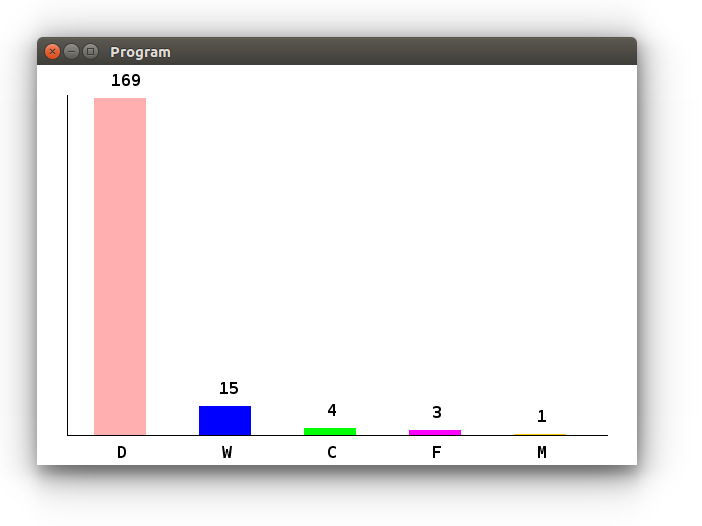
\includegraphics[width=0.9\textwidth]{../img/survey/bar}

\vspace{2em}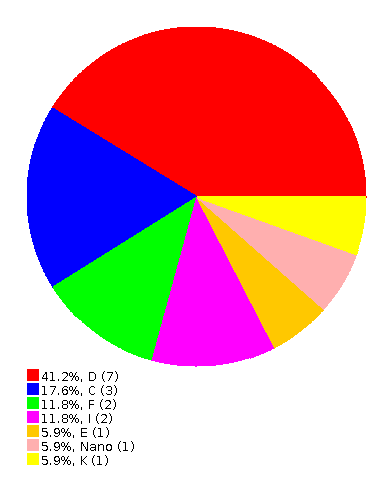
\includegraphics[width=0.7\textwidth]{../img/survey/pie}
\end{minipage}
\end{Slide}


\fi












%!TEX encoding = UTF-8 Unicode
%!TEX root = ../lect-w12.tex

%%%


\Subsection{Repetition: Vad är en algoritm?}
\begin{Slide}{Repetition: Vad är en algoritm? }\SlideFontTiny
\pause En \href{https://sv.wikipedia.org/wiki/Algoritm}{algoritm} är en stegvis beskrivning av hur man löser ett problem. \\ 
Exempel: SWAP, MIN, Registrering, Sökning, Sortering \\
\pause\vspace{0.5em}
Problemlösningsprocessens olika steg (inte nödvändigtvis i denna ordning): 
\begin{itemize}
\item Dela upp problemet i enklare delproblem och sätt samman.
\item Finns redan färdig lösning på (del)problem?
\item Formulera (del)\Emph{problemet} och ange tydligt indata och utdata: \\ exempel MIN: indata: sekvens av heltal; utdata: minsta talet
\item Kom på en \Emph{lösningsidé}: (kan  vara mycket klurigt och svårt) \\ exempel MIN: iterera över talen och håll reda på ''minst hittills''
\item Formulera en \Emph{stegvis beskrivning} som löser problemet: \\ exempel: pseudo-kod med sekvens av instruktioner
\item Implementera en \Emph{körbar lösning} i ''riktig'' kod: \\ exempel: en Scala-metod i en klass eller i ett singelobjekt
\item Har algoritmen acceptabel komplexitet i förhållande till tids- och minneskrav?
\end{itemize}
\pause Det krävs ofta \Emph{kreativitiet} i stegen ovan  -- även i att \Emph{känna igen} problemet!\\
Simpelt exempel: Du stöter på problemet MAX och ser likheten med MIN.\\
\pause\vspace{0.5em}\Emph{Övning}: Diskutera hur du löser detta problem i relation till stegen ovan: \\
\emph{Att räkna antalet förekomster av olika unika ord i en textsträng.} 
\end{Slide}













%!TEX encoding = UTF-8 Unicode
%!TEX root = ../lect-week11.tex

%%%

\ifkompendium\else

\Subsection{Jämföra strängar}

\begin{Slide}{Att jämföra strängar lexikografiskt}\SlideFontSmall
Teckenstandard \href{https://sv.wikipedia.org/wiki/UTF-16}{UTF-16}: Alla stora bokstäver är ''mindre'' än alla små:
\begin{REPLnonum}
scala> Array("hej","Hej","gurka").sorted
\end{REPLnonum}
\pause\vspace{-1.2em}
\begin{REPLnonum}
res0: Array[String] = Array(Hej, gurka, hej)\end{REPLnonum}
\pause
\begin{itemize}
\item Antag att vi vill lösa detta problem ''från scratch'': \\ \Emph{att sortera en sekvens med strängar} 
\item För att göra detta behöver vi lösa dessa delproblemen: 
\begin{itemize}
\item \Emph{att} \Alert{jämföra strängar}
\item \Emph{sökning i sekvenser}
\item \Emph{SWAP} (om på-plats-sortering i förändringsbar sekvens)
\end{itemize}
\item Vad betyder det att två strängar är ''lika''?

\item Vad betyder det att en sträng är ''mindre'' än en annan?
\end{itemize}
\pause {\SlideFontTiny Vi använder här strängjämförelse, sökning och sortering för att illustrera typiska \Emph{imperativa algoritmer}. \Alert{Normalt} använder man \Emph{färdiga lösningar} på dessa problem!}

\end{Slide}

\begin{Slide}{Jämföra strängar: likhet}\SlideFontSmall
Antag att vi inte kan göra \code{s1 == s2} utan bara kan jämföra strängar tecken för tecken, 
t.ex. så här: \code{s1(i) == s2(i)}. Antag också att vi inte har tillgång till annat än metoderna \code{length} och \code{apply} på strängar, samt  \code{while} och variabler av grundtyp. \Emph{Lös problemet att \emph{avgöra om två strängar är lika}.}

\pause
\begin{itemize}
\item Indata: två strängar
\item Utdata: \code{true} om lika annars \code{false}
\end{itemize}
\begin{enumerate}
\item Klura ut din lösningsidé
\item Formulera algoritmen i pseudokod
\item Implementera algoritmen i Scala: \code{def isEqual(s1: String, s2: String): Boolean} = ???
\end{enumerate}
\end{Slide}

\begin{Slide}{Algoritmexempel: stränglikhet, pseudokod}
\begin{Code}
def isEqual(s1: String, s2: String): Boolean = {
  if (/* lika längder */) {
    var foundDiff = false
    var i = /* första index */
    while (!foundDiff && /* i inom indexgräns */) {
      if (/* tecken på plats i är olika */) foundDiff = true
      else i = /* nästa index */
    }
    !foundDiff
  } else false
}
\end{Code}

\pause Detta är en variant av s.k. \Emph{linjärsökning} där vi söker från början i en sekvens till vi hittar det vi söker efter (här söker vi efter tecken som skiljer sig åt). 
\\\pause\vspace{2.5em} Hur ser implementationen i exekverbar Scala ut?
\end{Slide}

\begin{Slide}{Algoritmexempel: stränglikhet, implementation}\SlideFontSmall
\begin{Code}
def isEqual(s1: String, s2: String): Boolean = {
  if (s1.length == s2.length) {
    var foundDiff = false
    var i = 0
    while (!foundDiff && i < s1.length) {
      if (s1(i) != s2(i)) foundDiff = true
      else i += 1
    }
    !foundDiff
  } else false
}
\end{Code}
\pause 
{\SlideFontTiny Fördjupning: jämför ovan med implementationen av \code{String.equals} här:
\href{http://hg.openjdk.java.net/jdk8u/jdk8u60/jdk/file/935758609767/src/share/classes/java/lang/String.java#l976}{hg.openjdk.java.net/jdk8u/jdk8u60/jdk/file/935758609767/src/share/classes/java} \\ och använd \code{timed} nedan och jämför prestanda med \code{isEqual} ovan.\\
Obs! Mät många gånger så att JVM:en optimerar din kod.}
\vspace{-0.25em}\begin{Code}
def timed[T](block: => T): (Double, T) = { 
  val (t, res) = (System.nanoTime, block)
  ((System.nanoTime - t) / 1e9, res) 
}
\end{Code}

\end{Slide}

\begin{Slide}{Algoritmexempel: stränglikhet, prestanda}
\begin{REPL}
scala> val enMiljon = 1000000

scala> val s = Array.fill(enMiljon)('x').mkString

scala> val t = s.updated(enMiljon - 1, 'y')

scala> timed { s == t }
res42: (Double, Boolean) = (3.76459E-4,false)

scala> timed { isEqual(s,t) } 
res43: (Double, Boolean) = (3.31597E-4,false)
\end{REPL}
Ovan är kört efter ''uppvärmning'' på i7-4790K CPU @ 4.00GHz \\
Skillnaden inom mätfelmarginalen!
\end{Slide}



\begin{Slide}{Jämföra strängar: ''mindre än''}\SlideFontSmall
Med \code{s1 < s2} menar vi att strängen s1 ska sorteras före strängen s2 enligt hur de enskilda tecknen är ordnade med uttrycket \code{s1(i) < s2(i)}. \\
Antag också att vi inte har tillgång till annat än metoderna \code{length} och \code{apply} på strängar, samt  \code{while} och variabler av grundtyp, samt \code{math.min}
\\\Emph{Lös problemet att \emph{avgöra om en sträng är ''mindre'' än en annan}.}\\
\begin{itemize}
\item Indata: två strängar, s1, s2
\item Utdata: \code{true} om s1 ska sorteras före s2 annars \code{false}
\end{itemize}
\begin{enumerate}
\item Klura ut din lösningsidé
\item Formulera algoritmen i pseudokod
\item Implementera algoritmen i Scala: \code{def isLessThan(s1: String, s2: String): Boolean} = ???
\end{enumerate}
\end{Slide}

\begin{Slide}{Jämföra strängar: ''mindre än''}\SlideFontSmall
Pseudokod:
\begin{Code}
def isLessThan(s1: String, s2: String): Boolean = {
  
  val minLength = /* minimum av längderna på s1 och s2 */
  
  def firstDiff(s1: String, s2: String): Int = 
    /* index för första skillnaden (om de börjar lika: minLength) */

  val diffIndex = firstDiff(s1, s2)
  if (diffIndex == minLength) /* s1 är kortare än s2 */
  else /* tecknet s1(diffIndex) är mindre än tecknet s2(diffIndex) */ 
}
\end{Code}
\end{Slide}

\begin{Slide}{Jämföra strängar: ''mindre än''}\SlideFontSmall
\begin{Code}
def isLessThan(s1: String, s2: String): Boolean = {

  val minLength = math.min(s1.length, s2.length)

  def firstDiff(s1: String, s2: String): Int = {
    var foundDiff = false
    var i = 0
    while (!foundDiff && i < minLength) 
      if (s1(i) != s2(i)) foundDiff = true 
      else i += 1
    i
  }

  val diffIndex = firstDiff(s1, s2)
  if (diffIndex == minLength) s1.length < s2.length
  else s1(diffIndex) < s2(diffIndex)
}
\end{Code}
\end{Slide}

\begin{Slide}{Jämföra strängar i Java}\SlideFontTiny
\begin{itemize}
\item I Java kan man \Alert{inte} jämföra strängar med operatorerna \code{<}, \code{<=}, \code{>}, och \code{>=}

\item Dessutom ger operatorerna \code{==} och \code{!=} \emph{inte} innehålls(o)likhet utan \Alert{referens(o)likhet} \code{:(}

\item Istället \Alert{måste} man i Java använda metoderna \code{equals} och \code{compareTo} 
\\Dessa fungerar även i Scala eftersom strängar i Scala och Java är av samma typ, nämligen \code{java.lang.String}.
\pause
\item \code{s1.compareTo(s2)} ger ett heltal som är:
\begin{itemize}\SlideFontTiny
\item \code{0} om s1 och s2 har samma innehåll
\item \Alert{negativt} om s1 < s2 i lexikografisk mening, alltså s1 ska sorteras \Alert{före}
\item \Emph{positivt} om s1 > s2 i lexikografisk mening, alltså s1 ska sorteras \Emph{efter}
\end{itemize}

\pause
\item Undersök följande:
\begin{REPL}
scala> new String("hej") eq new String("hej") // motsvarar == i Java
scala> "hej".equals("hej")                    // samma som == i Scala
scala> "hej".compareTo("hej")
scala> "hej".compareTo("HEJ")         // alla stora är 'före' alla små
scala> "HEJ".compareTo("hej")
\end{REPL}
\end{itemize}

\href{http://docs.oracle.com/javase/8/docs/api/java/lang/String.html#compareTo-java.lang.String-}{docs.oracle.com/javase/8/docs/api/java/lang/String.html\#compareTo-java.lang.String-}
\end{Slide}


\begin{Slide}{Jämföra strängar i Java: exempel}\SlideFontSmall
Vad skriver detta Java-program ut?
\javainputlisting{../compendium/examples/StringEqTest.java}
\pause
\begin{REPL}
$ javac StringEqTest.java 
$ java StringEqTest 
false
true
0
\end{REPL}
\end{Slide}


\fi












%!TEX encoding = UTF-8 Unicode
%!TEX root = ../lect-week11.tex

%%%

\ifkompendium\else

\Subsection{Jämförelse Scala och Java}
\begin{Slide}{Grundläggande likheter och skillnader}\SlideFontSmall

\begin{itemize}
\item \Emph{Sökning} återkommer i många skepnader: \\ i en datastruktur, vilken det än må vara, vill man ofta kunna \\ \Emph{hitta ett element med en viss egenskap}. 

\pause
Några färdiga linjärsökningar i Scalas standardbibliotek:

\begin{REPL}
scala> Vector("gurka","tomat","broccoli").indexOf("tomat")
res0: Int = 1

scala> Vector("gurka","tomat","broccoli").indexWhere(_.contains("o"))
res1: Int = 1

scala> Vector("gurka","tomat","broccoli").find(_.contains("o"))
res2: Option[String] = Some(tomat)
\end{REPL}

\pause
\item Sökning efter ett visst index i en sekvens:

\begin{itemize}\SlideFontTiny
\item Indata: en sekvens och ett \Emph{sökkriterium}
\item Utdata: index för första eftersökta element, annars -1 
\end{itemize}

\pause
\item Två typiska varianter av sökning i en sekvens:
\begin{itemize}\SlideFontTiny
\item Linjärsökning: börja från början och sök tills ett eftersökt element är funnet
\item Binärsökning: antag sorterad sekvensen; börja i mitten, välj rätt halva ...
\end{itemize}
\end{itemize}
\end{Slide}

\Subsection{Linjärsökning}

\begin{Slide}{Linjärsökning: hitta index för elementet 42}
Skriv pseudokod för:\\ \code{def indexOf42(xs: Vector[Int]): Int = ???}
\pause
\begin{Code}
def indexOf42(xs: Vector[Int]): Int = {
  var i = /* index för första elementet */
  var found = false
  while (!found && /* index inom indexgräns */) {
    if (/* element på plats i är 42 */) found = true 
    else i = /* nästa index */
  }
  if (/* hittat */) i else -1
} 
\end{Code}
\end{Slide}

\begin{Slide}{Linjärsökning: hitta index för elementet 42}
Implementera:\\ \code{def indexOf42(xs: Vector[Int]): Int = ???}
\pause
\begin{Code}
def indexOf42(xs: Vector[Int]): Int = {
  var i = 0
  var found = false
  while (!found && i < xs.length) {
    if (xs(i) == 42) found = true 
    else i += 1
  }
  if (found) i else -1
} 
\end{Code}
\end{Slide}

\begin{Slide}{Linjärsökning: hitta index för elementet x}
Implementera:\\ \code{def indexOf(xs: Vector[Int], x: Int): Int = ???}
\pause
\begin{Code}
def indexOf(xs: Vector[Int], x: Int): Int = {
  var i = 0
  var found = false
  while (!found && i < xs.length) {
    if (xs(i) == x) found = true 
    else i += 1
  }
  if (found) i else -1
} 
\end{Code}
\end{Slide}

\begin{Slide}{Linjärsökning: hitta index för elementet p(x)}\SlideFontSmall
Implementera:\\ \code{def indexWhere(xs: Vector[Int], p: Int => Boolean): Int = ???}
\pause
\begin{Code}
def indexWhere(xs: Vector[Int], p: Int => Boolean): Int = {
  var i = 0
  var found = false
  while (!found && i < xs.length) {
    if (p(xs(i))) found = true 
    else i += 1
  }
  if (found) i else -1
} 
\end{Code}
\end{Slide}

\begin{Slide}{Linjärsökning: generalisera till godtycklig typ}\SlideFontSmall
Implementera:\\ \code{def indexWhere[T](xs: Vector[T], p: T => Boolean): Int = ???}
\pause
\begin{Code}
def indexWhere[T](xs: Vector[T], p: T => Boolean): Int = {
  var i = 0
  var found = false
  while (!found && i < xs.length) {
    if (p(xs(i))) found = true 
    else i += 1
  }
  if (found) i else -1
} 
\end{Code}
\end{Slide}

\begin{Slide}{Linjärsökning: generalisera till godtycklig typ}\SlideFontSmall
Typinferensen fungerar bättre om stegad funktion:\\ 
\code{def indexWhere[T](xs: Vector[T])(p: T => Boolean): Int}
\begin{Code}
def indexWhere[T](xs: Vector[T])(p: T => Boolean): Int = {
  var i = 0
  var found = false
  while (!found && i < xs.length) {
    if (p(xs(i))) found = true 
    else i += 1
  }
  if (found) i else -1
} 
\end{Code}
\end{Slide}


\begin{Slide}{Linjärsökning: generalisera till godtycklig sekvens}\SlideFontSmall
Implementera:\\ \code{def indexWhere[T](xs: Seq[T])(p: T => Boolean): Int = ???}
\pause
\begin{Code}
def indexWhere[T](xs: Seq[T])(p: T => Boolean): Int = {
  var i = 0
  var found = false
  while (!found && i < xs.length) {
    if (p(xs(i))) found = true 
    else i += 1
  }
  if (found) i else -1
} 
\end{Code}
\end{Slide}

\begin{Slide}{Linjärsökning: generalisera till godtycklig sekvens}\SlideFontSmall
Implementera:\\ \code{def find[T](xs: Seq[T])(p: T => Boolean): Option[T] = ???}
\pause
\begin{Code}
def find[T](xs: Seq[T])(p: T => Boolean): Option[T] = {
  var i = 0
  var found = false
  while (!found && i < xs.length) {
    if (p(xs(i))) found = true 
    else i += 1
  }
  if (found) Some(xs(i)) else None
} 
\end{Code}
\end{Slide}

\Subsection{Binärsökning}

\begin{Slide}{Binärsökning: snabbare men kräver sorterad sekvens}
\begin{REPL}[basicstyle=\color{white}\ttfamily\SlideFontSize{6.5}{8}]
scala> val enMiljon = 1000000

scala> val xs = Array.tabulate(enMiljon)(i => i + 1)   // sorterad

scala> xs(enMiljon - 1)
res0: Int = 1000000

scala> timed { xs.indexOf(enMiljon) }        // linjärsökning
res42: (Double, Int) = (0.016622994,999999)

scala> import scala.collection.Searching._  // ger tillgång till metoden search
import scala.collection.Searching._

scala> timed { xs.search(enMiljon) }        // binärsökning
res54: (Double, collection.Searching.SearchResult) = (2.45691E-4,Found(999999))

\end{REPL}
\pause
Citat från scaladoc för \code{search}:\\
''The sequence \Alert{should be sorted} before calling; otherwise, the results are \Alert{undefined.}''
\end{Slide}

\begin{Slide}{Binärsökning: lösningsidé}
\Emph{Problemlösningsidé}: Om sekvensen är sorterad kan vi utnyttja detta för en mer effektiv sökning, genom att jämföra med mittersta värdet och se om det vi söker finns före eller efter detta, och upprepa med ''halverad'' sekvens tills funnet.
\pause
\begin{itemize}\SlideFontSmall
\item \Emph{Indata}: sorterad sekvens av heltal och det eftersökta elementet
\item \Emph{Utdata}: \code{Found(index)} för det eftersökta elementet
\\ om saknas: \code{InsertionPoint(index)}
\pause
\begin{Code}
sealed trait SearchResult {
  def insertionPoint: Int
}

case class Found(foundIndex: Int) extends SearchResult {
  override def insertionPoint = foundIndex
}
  
case class InsertionPoint(insertionPoint: Int) extends SearchResult
\end{Code}
\end{itemize} 
\end{Slide}

\begin{Slide}{Binärsökning: pseudokod, iterativ lösning}
\Emph{Pseudo-kod}: iterativ lösning
\begin{Code}
def binarySearch(xs: Vector[Int])(elem: Int): SearchResult = {
  var found = false
  var (low, high) = (/* lägsta index */, /* högsta index */)
  var mid = /* något startvärde */ 
  while (!found && /* finns fler element kvar */) {
    mid = /* mittpunkten i intervallet (low, high) */
    if (xs(mid) == elem) found = true
    else if (xs(mid) < elem) /* flytta intervallets undre gräns */
    else /* flytta intervallets övre gräns" */
  }
  if (found) Found(mid)
  else InsertionPoint(low)
}
\end{Code}
\end{Slide}



\begin{Slide}{Binärsökning: implementation, iterativ lösning}
\Emph{Implementation}: iterativ lösning
\begin{Code}
def binarySearch(xs: Vector[Int])(elem: Int): SearchResult = {
  var found = false
  var (low, high) = (0, xs.length - 1)
  var mid = -1 
  while (!found && low <= high) {
    mid = (low + high) / 2
    if (xs(mid) == elem) found = true
    else if (xs(mid) < elem) low = mid + 1
    else high = mid - 1 
  }
  if (found) Found(mid) 
  else InsertionPoint(low)
}
\end{Code}
\end{Slide}

\begin{Slide}{Binärsökning: instrumentering av iterativ lösning}
\vspace{-0.5em}
\begin{CodeSmall}
def waitForEnter: Unit = scala.io.StdIn.readLine("")
def show(msg: String): Unit = {println(msg); waitForEnter}

def binarySearch(xs: Vector[Int])(elem: Int): SearchResult = {
  var found = false                         ; show(s"found = $found")
  var (low, high) = (0, xs.length - 1)      ; show(s"(low, high) = ($low, $high)")
  var mid = -1                              ; show(s"mid = $mid")
  while (!found && low <= high) {           ; show(s"while ${!found && low <= high}")
    mid = (low + high) / 2                  ; show(s"mid = $mid")
    if (xs(mid) == elem) {found = true      ; show(s"found = $found")}
    else if (xs(mid) < elem) {low = mid + 1 ; show(s"low = $low")}
    else {high = mid - 1                    ; show(s"high = $high")}
  }
  if (found) Found(mid) 
  else InsertionPoint(low)
}
\end{CodeSmall}
\vspace{-0.5em}
\begin{REPL}[basicstyle=\color{white}\ttfamily\SlideFontSize{6}{7}]
scala> binarySearch(Vector(0,1,2,3,42,5))(42)
found = false
(low, high) = (0, 5)
mid = -1
while true
mid = 2
low = 3
while true
mid = 4
found = true
res0: collection.Searching.SearchResult = Found(4)
\end{REPL}
\end{Slide}

\begin{Slide}{Binärsökning: rekursiv lösning}
\Emph{Fördjupning}: rekursiv lösning
\begin{Code}
def binarySearch(xs: Vector[Int])(elem: Int): SearchResult = {
  def loop(low: Int, high: Int): SearchResult = 
    if (low > high) InsertionPoint(low) 
    else (low + high) / 2 match {
      case mid if xs(mid) == elem => Found(mid)
      case mid if xs(mid) < elem  => loop(mid + 1, high)
      case mid                    => loop(low, mid - 1)
    }
    
  loop(0, xs.length - 1) 
}
\end{Code}
\end{Slide}


\begin{Slide}{Binärsökning: generisk rekursiv lösning}
\Emph{Fördjupning}: iterativ generisk lösning med implicit ordning
\begin{CodeSmall}
def binarySearch[T](xs: Seq[T])(elem: T)(implicit ord: Ordering[T]): SearchResult = {
  import ord._
  def loop(low: Int, high: Int): SearchResult = 
    if (low > high) InsertionPoint(low) 
    else (low + high) / 2 match {
      case mid if xs(mid) == elem => Found(mid)
      case mid if xs(mid) < elem  => loop(mid + 1, high)
      case mid                    => loop(low, mid - 1)
    }
    
  loop(0, xs.length - 1) 
}
\end{CodeSmall}
{\SlideFontSmall För den intresserade:\\Se fördjupningsuppgifter om implicita ordningar i veckans övning.}
\end{Slide}

\begin{Slide}{Tidskomplexitet, sökning}\SlideFontSmall

\Emph{Fördjupning:}\\Algoritmteoretisk analys av sökalgoritmerna ger:
\begin{itemize}
\item Linjärsökning: tiden är proportionell mot $n$, skrivs: $O(n)$ 
\item Binärsökning:  tiden är proportionell mot $\log_2 n$, skrivs: $O(\log n)$
\end{itemize}
\vspace{1em}\pause
Empirisk analys: Vi har en vektor med 1000 element. Vi har mätt tiden för att söka upp ett element många gånger och funnit att det tar ungefär 1 $\mu$s både med linjärsökning och binärsökning. 
\\\vspace{1em}Hur lång tid tar det om vi har fler element i vektorn?\\
\vspace{1em}
\begin{tabular}{rccccc}
       & 1000 & 10 000 & 100000 & 1 000 000 & 10 000 000 \\ \hline
linjärsökning & 1     & 10     & 100     & 1000     & 10 000 \\
binärsökning  & 1     & 1.33   & 1.67    & 2.00     & 2.33
\end{tabular}
\vspace{1em} 

{\SlideFontTiny 

Kurserna: \\
''\Emph{Utvärdering av programvarusystem}'', obl. för D1, studerar detta \Alert{empiriskt}\\
''\Emph{Algoritmer, datastrukturer och komplexitet}'', obl. för D2, studerar detta \Alert{analytiskt}
}
\end{Slide} 


\fi











%!TEX encoding = UTF-8 Unicode
%!TEX root = ../lect-w12.tex

%%%

\Subsection{Sortering}


\begin{Slide}{Sorteringsproblemet}
\Emph{Problem}: Vi har en osorterad sekvens med heltal. Vi vill ordna denna osorterade sekvens i en sorterad sekvens från minst till störst.
\pause

\vspace{2em}
En \emph{generalisering} av problement: \\ \vspace{1em} Vi har många element av godtycklig typ och en \Emph{ordningsrelation} som säger vad vi menar med att ett element är \emph{mindre än} eller \emph{större än eller lika med} ett annat element. \\ \vspace{1em}
Vi vill lösa problemet att ordna elementen i sekvens så att för varje element på plats $i$ så är efterföljande element på plats $i + 1$ större eller lika med elementet på plats $i$.

\end{Slide}

\begin{Slide}{Två enkla sporteringsalgoritmer: \\ Insättningssortering \& Urvalssortering}
\begin{itemize}
\item Insättningssortering \Emph{lösningsidé}: Ta ett element i taget från den osorterade listan och \Alert{sätt in} det på \Alert{rätt plats} i den sorterade listan och upprepa till det inte finns fler osorterade element.
\pause
\item Urvalsssortering \Emph{lösningsidé}: \Alert{Välj ut} det minsta kvarvarande elementet i den osorterade listan och placera det \Alert{sist} i den sorterade listan och upprepa till det inte finns fler osorterade element.
\end{itemize}
\end{Slide}



\begin{Slide}{Tidskomplexitet, sortering, medeltal}
\begin{tabular}{ll}
Urvalssortering, insättningssortering: & $O(n^2)$ \\
''Bra'' metoder, tex Quicksort, Timsort:  & $O(n\log n)$
\end{tabular}

\vspace{1em}\footnotesize
Vi har en vektor med 1000 element. Vi har mätt tiden för att sortera elementen många gånger och funnit att det tar ungefär 1 ms både med urvalssortering (eller någon annan ''dålig'' metod) och en ''bra'' metod. Hur lång tid tar det om vi har fler element i vektorn?

\vspace{1em}
\begin{tabular}{rccccc}
       & 1,000 & 10,000 & 100,000 & 1,000,000 & 10,000,000 \\ \hline
dålig  & 1     & 100    & $10^4$  & $10^6$   & $10^8$ \\
bra    & 1     & 13.3   & 167     & 2000     & 23000
\end{tabular}
\end{Slide}

\begin{Slide}{Bogo sort}
\begin{Code}
def bogoSort(xs: Vector[Int]) = {
  var result = xs
  while(result != result.sorted) {
    result = scala.util.Random.shuffle(result)
  }
  result
}
\end{Code}
När blir denna färdig? \pause \\
\url{https://en.wikipedia.org/wiki/Bogosort}\\
Antal jämförelser i medeltal vid många mätningar: $ O(n \cdot n!) $
\end{Slide}





\begin{Slide}{Det finns många olika sorteringsalgoritmer}
\begin{itemize}
\item Visualisering av 15 olika sorteringsalgoritmer på 6 min:\\{\SlideFontSmall\url{https://www.youtube.com/watch?v=kPRA0W1kECg}}
\item Olika sorteringsalgoritmer har olika tids- \& minneskomplexitet: i bästa fall, i värsta fall, i medeltal, för nästan sorterad, etc.
\\{\SlideFontSmall\url{https://en.wikipedia.org/wiki/Sorting_algorithm}}
\item Olika sorteringsalgoritmer lämpar sig olika väl för parallellisering på många kärnor.
\end{itemize}
\end{Slide}




\begin{Slide}{Insättnings- och urvalssortering}
\Emph{Insertion sort}
\begin{itemize}
\item Wikipedia:\\
{\SlideFontSmall\url{https://sv.wikipedia.org/wiki/Insättningssortering}}
{\SlideFontSmall\url{https://en.wikipedia.org/wiki/Insertion_sort}}

\item AlgoRythmics: Insert-sort with Romanian folk dance\\
{\SlideFontSmall\url{https://www.youtube.com/watch?v=ROalU379l3U}}
\end{itemize}

\vspace{2em}
\Emph{Selection sort}

\begin{itemize}
\item Wikipedia:\\ 
{\SlideFontSmall\url{https://sv.wikipedia.org/wiki/Urvalssortering}}\\
{\SlideFontSmall\url{https://en.wikipedia.org/wiki/Selection_sort}}

\item AlgoRythmics: Select-sort with Gypsy folk dance \\ 
{\SlideFontSmall\url{https://www.youtube.com/watch?v=Ns4TPTC8whw}}
\end{itemize}
\end{Slide}




\begin{Slide}{Sortera till ny vektor med insättningssortering: pseudo-kod}

{\SlideFontSmall Det är nog lättare att förstå \Emph{insertion sort} om man sorterar till en ny vektor. \\ Vi ska sedan se hur man sorterar ''på plats'' \Eng{in place} i en  array.\\} \vspace{1em}
\Emph{Indata}: en osorterad vektor med heltal \\
\Emph{Utdata}: en ny, sorterad vektor med heltal
\begin{Code}
def insertionSort(xs: Vector[Int]): Vector[Int] = {
  val sorted = /* tom ArrayBuffer */
  for (/* alla element i xs */) {
     /* linjärsök rätt position i sorted */
     /* sätt in element på rätt plats i sorted */
  }
  sorted.toVector
}
\end{Code}
\end{Slide}


\begin{Slide}{Sortera till ny vektor med insättningssortering: implementation i Scala}
\begin{Code}
def insertionSort(xs: Vector[Int]): Vector[Int] = {
  val sorted = scala.collection.mutable.ArrayBuffer.empty[Int]
  for (elem <- xs) {
     // linjärsök rätt position i sorted:
     var pos = 0
     while (pos < sorted.length && sorted(pos) < elem) {
       pos += 1
     }
     // sätt in element på rätt plats i sorted:
     sorted.insert(pos, elem)
  }
  sorted.toVector
}
\end{Code}
\end{Slide}

\begin{Slide}{Sortera till ny vektor med insättningssortering: implementation i Java med foreach-sats}
\SlideFontTiny\vspace{-0.5em}
\begin{Code}[language=Java]
import java.util.ArrayList;

public class JSort {
    public static ArrayList<Integer> insertionSort(ArrayList<Integer> xs) {
        ArrayList<Integer> sorted = new ArrayList<Integer>();
        for (int elem : xs) {
            // linjärsök rätt position i sorted:
            int pos = 0;
            while (pos < sorted.size() && sorted.get(pos) < elem) {
                pos++;
            }
            // sätt in element på rätt plats i sorted:
            sorted.add(pos, elem);
        }
        return sorted;
    }
}
\end{Code}
\vspace{-0.3em}
\href{http://stackoverflow.com/questions/85190/how-does-the-java-for-each-loop-work}{ stackoverflow.com/questions/85190/how-does-the-java-for-each-loop-work}

Javasamlingar måste ''wrappa'' primitiva \jcode{int} i klassen \code{Integer} (mer om detta senare)
\end{Slide}

\begin{Slide}{Sortera till ny vektor med urvalssortering: pseudo-kod}

{\SlideFontSmall Det är nog lättare att förstå \Emph{selection sort} om man sorterar till en ny vektor. \\ Vi ska sedan se hur man sorterar ''på plats'' \Eng{in place} i en  array.\\} \vspace{1em}
\Emph{Indata}: en osorterad vektor med heltal \\
\Emph{Utdata}: en sorterad vektor med heltal
\begin{Code}
def selectionSort(xs: Vector[Int]): Vector[Int] = {
  val unsorted = xs.toBuffer
  val sorted = scala.collection.mutable.ArrayBuffer.empty[Int]
  while (/* unsorted inte är tom */) {
    var indexOfMin = /* index för minsta element i unsorted */
    /* flytta elementet unsorted(indexOfMin) till sist i sorted */
  }
}
\end{Code}
\end{Slide}

\begin{Slide}{Sortera till ny vektor med urvalssortering: implementation i Scala}
\SlideFontTiny\vspace{-0.5em}
\begin{Code}
def selectionSort(xs: Vector[Int]): Vector[Int] = {
  val unsorted = xs.toBuffer
  val sorted = scala.collection.mutable.ArrayBuffer.empty[Int]
  while (unsorted.nonEmpty) {
    var indexOfMin = 0
    // index för minsta element i unsorted:
    for (i <- 1 until unsorted.length) {
      if (unsorted(i) < unsorted(indexOfMin)) indexOfMin = i
    }
    val elem = unsorted.remove(indexOfMin)  // ta bort ur unsorted
    sorted.append(elem)  // lägg sist i sekvensen med sorterade
  }
  sorted.toVector
}
\end{Code}
\pause
\begin{itemize}
\item Funkar tom sekvens?
\item Funkar en sekvens med ett element?
\item Funkar det för osorterad sekvens med (minst) två element?
\item Vad händer om sekvensen är sorterad?
\end{itemize}
\end{Slide}

\begin{Slide}{Sortera till ny vektor med urvalssortering: implementation i Java}
\begin{Code}[language=Java]
public static ArrayList<Integer> selectionSort(ArrayList<Integer> unsorted) {
    ArrayList<Integer> sorted = new ArrayList<Integer>();
    while (unsorted.size() > 0) {
        int indexOfMin = 0;
        // index för minsta element i unsorted:
        for (int i = 1; i < unsorted.size(); i++) {
            if (unsorted.get(i) < unsorted.get(indexOfMin)) {
                indexOfMin = i;
            }
        }
        int elem = unsorted.remove(indexOfMin);  // ta bort ur unsorted
        sorted.add(elem);  // lägg sist i sekvensen med sorterade
    }
    return sorted;
}
\end{Code}
OBS! Ovan algoritm ''\Alert{förstör}'' innehållet i inparametern! \\ Hur förhindra det?
\end{Slide}

\begin{Slide}{Sortera till ny vektor med urvalssortering: implementation i Java}
\begin{Code}[language=Java]
public static ArrayList<Integer> selectionSort(ArrayList<Integer> xs) {
    ArrayList<Integer> unsorted = new ArrayList<Integer>(xs); //ref copy
    ArrayList<Integer> sorted = new ArrayList<Integer>();
    while (unsorted.size() > 0) {
        int indexOfMin = 0;
        // index för minsta element i unsorted:
        for (int i = 1; i < unsorted.size(); i++) {
            if (unsorted.get(i) < unsorted.get(indexOfMin)) {
                indexOfMin = i;
            }
        }
        int x = unsorted.remove(indexOfMin);  // ta bort ur unsorted
        sorted.add(x);  // lägg sist i sekvensen med sorterade
    }
    return sorted;
}
\end{Code}
\end{Slide}

\begin{Slide}{Urvalssortering på plats: pseudo-kod}
\Emph{Indata:} en array med heltal\\
\Emph{Utdata:} samma array, men nu sorterad\\

\begin{Code}
def selectionSortInPlace(xs: Array[Int]): Unit = {
  def minIndex(fromIndex: Int): Int = {
    /* index för minsta element från fromIndex  */
  }

  for (i <- /* från första till NÄST sista index */) {
    /* byt plats mellan xs[i] och xs[minIndex(i)] */
  }
}
\end{Code}
\pause
Se animering här: \href{https://sv.wikipedia.org/wiki/Urvalssortering}{Urvalssortering på Wikipedia}
\end{Slide}

\begin{Slide}{Urvalssortering på plats: implementation i Scala}\SlideFontSmall
\vspace{-0.25em}
\Emph{Indata:} en array med heltal\\
\Emph{Utdata:} samma array, men nu sorterad\\

\begin{Code}[numberstyle=\ttfamily\SlideFontSize{6}{7.5},numbers=left]
def selectionSortInPlace(xs: Array[Int]): Unit = {
  def minIndex(fromIndex: Int): Int = {
    var result = fromIndex
    for (i <- fromIndex + 1 until xs.length) {
      if (xs(i) < xs(result)) result = i
    }
    result
  }

  def swap(i: Int, j: Int): Unit = {
    val temp = xs(i)
    xs(i) = xs(j)
    xs(j) = temp
  }

  for (i <- 0 until xs.length - 1) { // till NÄST sista
    swap(i, minIndex(i))
  }
}
\end{Code}
\end{Slide}

\begin{Slide}{Selection sort, in place, Java}\SlideFontTiny
Om man ''slår ihop'' del-lösningarna minIndex och swap så kan man skriva detta lite kortare och utnyttja att variablen min nedan kan användas i stället för temp.  \\
OBS! Det är viktigare att koden är lättläst än att den är kort och koden optimeras åt oss av kompilatorn och/eller JVM så extra variabler och funktionsanrop är sällan problem.
\begin{Code}[language=Java,basicstyle=\ttfamily\SlideFontSize{6}{7.5},numberstyle=\ttfamily\SlideFontSize{6}{8}, numbers=left]
public static void selectionSortInPlace(int[] xs) {
    for (int i = 0; i < xs.length - 1; i++) {
        int min = Integer.MAX_VALUE;
        int minIndex = -1;
        for (int k = i; k < xs.length; k++) {
            if (xs[k] < min) {
                min = xs[k];
                minIndex = k;
            }
        }
        xs[minIndex] = xs[i];
        xs[i] = min;
    }
}
\end{Code}


\pause Det finns ett specialfall som kommer krascha denna implementation. Vilket?
\pause\\\jcode|new int[]{Integer.MAX_VALUE, Integer.MAX_VALUE}|
\end{Slide}

\begin{Slide}{Insättningssortering på plats -- pseudo-kod}
\Emph{Indata:} en array med heltal\\
\Emph{Utdata:} samma array, men nu sorterad\\
\begin{Code}
def insertionSortInPlace(xs: Array[Int]): Unit = {
  for (i <- 1 until xs.length) {  //från ANDRA till sista
    var j = i
    while (j > 0 && xs(j - 1) > xs(j)) {
      /* byt plats på xs(j) och xs(j - 1) */
      j -= 1;  // stega bakåt
    }
  }
}
\end{Code}
\pause
Se animering här: \href{https://sv.wikipedia.org/wiki/Ins\%C3\%A4ttningssortering}{Insättningssortering på wikipedia}\\
Gå igenom alla specialfall och kolla så att detta fungerar!
\end{Slide}

\begin{Slide}{Insertion sort, in place, Scala}
\begin{Code}
def insertionSortInPlaceSwap(xs: Array[Int]): Unit = {
  def swap(i: Int, j: Int): Unit = {
    val temp = xs(i)
    xs(i) = xs(j)
    xs(j) = temp
  }
  for (i <- 1 until xs.length) {  //från ANDRA till sista
    var j = i
    while (j > 0 && xs(j - 1) > xs(j)) {
      swap(j, j - 1)
      j -= 1;  // stega bakåt
    }
  }
}
\end{Code}
\end{Slide}


\begin{Slide}{Insertion sort, in place, with swap, Java}
Vi kan tyvärr inte ha lokala funktioner i Java.
\begin{Code}[language=Java]
private void swap(int[] xs, int a, int b) {
    int temp = xs[a];
    xs[a] = xs[b];
    xs[b] = temp;
}

public void insertionSortInPlaceSwap(int[] xs) {
    for (int i = 1; i < xs.length; i++) {
        int j = i;
        while (j > 0 && xs[j - 1] > xs[j]) {
            swap(xs, j, j - 1);
            j = j - 1;
        }
    }
}
\end{Code}
\end{Slide}

\begin{Slide}{Insertion sort, in place, kortare implementation}
Kortare! Men kanske inte mer lättläst?
\begin{Code}[language=Java]
    public void insertionSortInPlace(int[] xs) {
        for (int i = 1; i < xs.length; i++) {
            int current = xs[i];
            int j = i;
            while (j > 0 && xs[j - 1] > current) {
                xs[j] = xs[j - 1];
                j--;
            }
            xs[j] = current;
        }
    }
\end{Code}

\end{Slide}




\begin{Slide}{Sortera samlingar med godtyckligt ordningspredikat}
\begin{Code}
def sortWith(xs: Vector[Int])(lt: (Int, Int) => Boolean ): Vector[Int] = {
  val sorted = scala.collection.mutable.ArrayBuffer.empty[Int]
  for (elem <- xs) {  // insertion sort using lt as "less than"
     var pos = 0
     while (pos < sorted.length && lt(sorted(pos), elem)) {
       pos += 1
     }
     sorted.insert(pos, elem)
  }
  sorted.toVector
}
\end{Code}
\pause
\begin{REPL}
scala> val xs = Vector(1,2,1,2,12,42,1)
xs: scala.collection.immutable.Vector[Int] = Vector(1, 2, 1, 2, 12, 42, 1)

scala> sortWith(xs)(_ < _)
res0: Vector[Int] = Vector(1, 1, 1, 2, 2, 12, 42)

scala> sortWith(xs)(_ > _)
res1: Vector[Int] = Vector(42, 12, 2, 2, 1, 1, 1)
\end{REPL}
\end{Slide}


\begin{Slide}{Fördjupning: Sortera samlingar av godtycklig typ}
\vspace{-0.25em}
\begin{Code}
def sortWith[T](xs: Vector[T])(lt: (T, T) => Boolean ): Vector[T] = {
  val sorted = scala.collection.mutable.ArrayBuffer.empty[T]
  for (elem <- xs) {
     var pos = 0
     while (pos < sorted.length && lt(sorted(pos), elem)) {
       pos += 1
     }
     sorted.insert(pos, elem)
  }
  sorted.toVector
}
\end{Code}
\pause\vspace{-0.25em}
\begin{REPL}
scala> case class Gurka(namn: String, vikt: Int)

scala> val xs = Vector(Gurka("a", 100), Gurka("b", 50), Gurka("c", 100))

scala> sortWith(xs)(_.vikt > _.vikt)
res0: Vector[Gurka] = Vector(Gurka(c,100), Gurka(a,100), Gurka(b,50))

scala> sortWith(xs)(_.vikt >= _.vikt)
res1: Vector[Gurka] = Vector(Gurka(a,100), Gurka(c,100), Gurka(b,50))
\end{REPL}
\end{Slide}


\begin{Slide}{Vad menas med att en sorteringsalgoritm är stabil?}
En sorteringsalgoritm är \Emph{stabil} om \Alert{ordningen} mellan element som anses \Emph{lika} enligt sorteringsordningsrelationen \Alert{bevaras}.\\\vspace{1em}
Fördjupning:
\href{https://en.wikipedia.org/wiki/Sorting_algorithm#Stability}
{en.wikipedia.org/wiki/Sorting\_algorithm\#Stability}
\end{Slide}

\begin{Slide}{Sortera samlingar med inbyggda sortBy och sortWith}
\begin{REPL}
scala> case class Gurka(namn: String, vikt: Int)
defined class Gurka

scala> val xs = Vector(Gurka("a", 100), Gurka("b", 50), Gurka("c", 100))

scala> xs.sortBy(_.vikt)
res0: scala.collection.immutable.Vector[Gurka] =
        Vector(Gurka(b,50), Gurka(a,100), Gurka(c,100))

scala> xs sortWith (_.vikt > _.vikt)
res1: scala.collection.immutable.Vector[Gurka] =
        Vector(Gurka(a,100), Gurka(c,100), Gurka(b,50))

\end{REPL}
\end{Slide}



\begin{Slide}{Fördjupning: sortera samlingar implicit ordning}
\begin{REPL}
scala> case class Gurka(namn: String, vikt: Int)
defined class Gurka

scala> val xs = Vector(Gurka("a", 100), Gurka("b", 50), Gurka("c", 100))

scala> xs.sorted
<console>:15: error: No implicit Ordering defined for Gurka.
       xs.sorted
          ^
\end{REPL}
\pause
Detta kan fixas genom att tillhandahålla en \Emph{implicit} ordning för \code{Gurka}:
\begin{Code}
implicit object minGurkOrdning extends Ordering[Gurka] {
  def compare(x: Gurka, y: Gurka): Int =
    if (x == y) 0
    else if (x.vikt < y.vikt) -1
    else 1
}
\end{Code}
\end{Slide}


\begin{Slide}{Fördjupning: sortera samlingar implicit ordning}
\begin{REPL}
scala> case class Gurka(namn: String, vikt: Int)
defined class Gurka

scala> val xs = Vector(Gurka("a", 100), Gurka("b", 50), Gurka("c", 100))

scala> implicit object minGurkOrdning extends Ordering[Gurka] {
         def compare(x: Gurka, y: Gurka): Int =
           if (x == y) 0
           else if (x.vikt < y.vikt) -1
           else 1
       }

scala> xs.sorted
res0: scala.collection.immutable.Vector[Gurka] =
        Vector(Gurka(b,50), Gurka(a,100), Gurka(c,100))
\end{REPL}
{\SlideFontTiny Se exempel på olika bekvämare sätt att definiera en ordning för dina egna typer: 
\url{https://stackoverflow.com/questions/19345030/easy-idiomatic-way-to-define-ordering-for-a-simple-case-class}}
\end{Slide}


\begin{Slide}{Vad kommer (inte) på tentan?}
Detta \Emph{kan} komma på tentan:
\begin{itemize}
\item Använda färdiga söknings- och sorteringsfunktioner på samlingar av specifik typ
\item Implementera egen linjärsökning i samlingar av specifik typ
\item Implementera egen binärsökning i samlingar av specifik typ
\item Implementera egen sortering till ny samling av specifik typ (du får själv välja algoritm, lämpligen insättnings- eller urvalssortering)

\end{itemize}
Detta kommer \Alert{inte} på tentan:
\begin{itemize}
\item Implementera generisk sökning
\item Implementera generisk sortering
\item Implementera sortering ''på plats''
\item Bogo sort
\end{itemize}
\end{Slide}


%\chapter{Trådar, Web, Android}
\begin{itemize}[nosep]
\item Thread
\item Future
\item HTML
\item Javascript
\item css
\item Scala.js
\item Android
\end{itemize}

%!TEX encoding = UTF-8 Unicode
%!TEX root = ../exercises.tex

\ifPreSolution

\Exercise{\ExeWeekTWELVE}\label{exe:W12}

\begin{Goals}
\item Förstå hur sorteringsordningen är definierad för strängar.
\item Förstå skillnaderna mellan strängjämförelser i Scala och Java, samt kunna jämföra strängar med jämförelsoperatorer i Scala och med \code{compareTo} i Java.
\item Kunna sortera sekvenssamlingar innehållande objekt av grundtyper med hjälp av inbyggda och egendefinierade sorteringsordningar med metoderna \code{sorted}, \code{sortBy} och \code{sortWith}.
\item Kunna använda inbyggda linjärsöknings- och binärsökningsmetoder.
\item Kunna implementera en egen sökalgoritm med linjärsökning och binärsökning.
\item Förstå när binärsökning är lämplig och möjlig.
\item Kunna implementera en enkel sorteringsalgoritm, t.ex. insättningssortering eller urvalssortering, både till ny samling och på plats.
\item Känna till hur implicita sorteringsordningar används för grundtyperna och egendefinierade typer.
\item Känna till existensen av, funktionen hos, och relationen mellan klasserna \code{Ordering} och \code{Comparator}, samt  \code{Ordered} och \code{Comparable}.
\end{Goals}

% \begin{Preparations}
% \item \StudyTheory{12}
% \end{Preparations}

\BasicTasks %%%%%%%%%%%%%%%%

\else

\ExerciseSolution{\ExeWeekTWELVE}

\BasicTasks

\fi





\WHAT{Jämföra strängar i Scala.}

\QUESTBEGIN

\Task \label{task:string-order-operators} \what~  I Scala kan strängar jämföras med operatorerna \code{==}, \code{!=}, \code{<}, \code{<=}, \code{>}, \code{>=},  där likhet/olikhet avgörs av om alla tecken i strängen är lika eller inte, medan större/mindre avgörs av sorteringsordningen i enlighet med varje teckens Unicode-värde.\footnote{Överkurs: Alla tecken i en \code{java.lang.String} representeras enligt UTF-16-standarden (\href{https://en.wikipedia.org/wiki/UTF-16}{https://en.wikipedia.org/wiki/UTF-16}), vilket innebär att varje Unicode-kodpunkt \Eng{code point} lagras som antingen ett eller två 16-bitars heltal. Strängjämförelse i Scala och Java jämför egentligen inte varje tecken, utan varje 16-bitars heltal. Denna skillnad har ingen betydelse när en sträng bara innehåller tecken som tar upp ett 16-bitars heltal var, och praktiskt nog är nästan alla tecken som används vardagligen av den typen. De flesta tecken som kräver två 16-bitars heltal är sällsynta kinesiska tecken, sällsynta symboler, tecken från utdöda språk och emoji. Vi kommer att bortse från sådana tecken i den här kursen.}

\Subtask Vad ger följande jämförelser för värde?
\begin{REPL}
scala> 'a' < 'b'
scala> "aaa" < "aaaa"
scala> "aaa" < "bbb"
scala> "AAA" < "aaa"
scala> "ÄÄÄ" < "ÖÖÖ"
scala> "ÅÅÅ" < "ÄÄÄ"
\end{REPL}
Tyvärr så följer ordningen av ÄÅÖ inte svenska regler, men det ignorerar vi i fortsättningen för enkelhets skull; om du är intresserad av hur man kan fixa  detta, gör uppgift \ref{task:swedish-letter-ordering}.

\Subtask\Pen Vilken av strängarna $s1$ och $s2$ kommer först (d.v.s. är ''mindre'') om $s1$ utgör början av $s2$ och $s2$ innehåller fler tecken än $s1$?


\SOLUTION


\TaskSolved \what


\SubtaskSolved
\begin{REPL}
true
true
true
true
true
false
\end{REPL}

\SubtaskSolved
\emph{s1} kommer först.


\QUESTEND





\WHAT{Jämföra strängar i Java.}

\QUESTBEGIN

\Task  \what~  I Java kan man \textbf{inte} jämföra strängar med operatorerna \code{<}, \code{<=}, \code{>}, och \code{>=}. Dessutom ger operatorerna \code{==} och \code{!=} inte innehålls(o)likhet utan referens(o)likhet. Istället får man använda metoderna \code{equals} och \code{compareTo}, vilka också fungerar i Scala eftersom strängar i Scala och Java är av samma typ, nämligen \code{java.lang.String}.


\Subtask Vad ger följande uttryck för värde?

\begin{REPL}
scala> "hej".getClass.getTypeName
scala> "hej".equals("hej")
scala> "hej".compareTo("hej")
\end{REPL}


\Subtask Studera dokumentationen för metoden \code{compareTo} i \code{java.lang.String}\footnote{\href{https://docs.oracle.com/javase/8/docs/api/java/lang/String.html\#compareTo-java.lang.String-}{docs.oracle.com/javase/8/docs/api/java/lang/String.html\#compareTo-java.lang.String-}} och skriv minst 3 olika uttryck i Scala REPL som testar hur metoden fungerar i olika fall.

\Subtask Studera dokumentationen \code{compareToIgnoreCase} \footnote{\href{https://docs.oracle.com/javase/8/docs/api/java/lang/String.html\#compareToIgnoreCase-java.lang.String-}{docs.oracle.com/javase/8/docs/api/java/lang/String.html\#compareToIgnoreCase-java.lang.String-}} och skriv minst 3 olika stränguttryck i Scala REPL som testar hur metoden fungerar i olika fall.

\Subtask Vad skriver följande Java-program ut?
\javainputlisting{examples/StringEqTest.java}


\SOLUTION


\TaskSolved \what

\SubtaskSolved
\begin{REPL}
String = java.lang.String
Boolean = true
Int = 0
\end{REPL}

\SubtaskSolved
Exempel på 3 olika uttryck för att testa \code{compareTo}:

\begin{enumerate}
\item
Hej kommer först då \code{H < h}.
\begin{REPLnonum}
	"hej".compareTo("Hej)
	res: Int = 32
\end{REPLnonum}

\item
Dessa är ekvivalenta, så \code{compareTo} returnerar 0.
\begin{REPLnonum}
	"hej".compareTo("hej")
	res: Int = 0
\end{REPLnonum}

\item
\emph{h} kommer före \emph{ö}.
\begin{REPLnonum}
	"hej".compareTo("ö")
	res: Int = -142
\end{REPLnonum}
\end{enumerate}

\SubtaskSolved
Exempel på 3 olika uttryck för att testa \code{compareToIgnoreCase}:

\begin{enumerate}

\item
\begin{REPLnonum}
	"hej".compareToIgnoreCase("HEj")
	res: Int = 0
\end{REPLnonum}

\item
\begin{REPLnonum}
	"hej".compareToIgnoreCase("Ö")
	res: Int = -142
\end{REPLnonum}

\item
Samma som ovan, då Ö omvandlas till ö innan jämförelse.
 \begin{REPLnonum}
	"hej".compareToIgnoreCase("ö") \\ res: Int = -142
\end{REPLnonum}
\end{enumerate}

\SubtaskSolved
\begin{REPL}
false
true
0
\end{REPL}



\QUESTEND





\WHAT{Sortering med inbyggda sorteringsmetoder.}

\QUESTBEGIN

\Task  \what~  För grundtyperna (\code{Int}, \code{Double}, \code{String}, etc.) finns en fördefinierad ordning som gör så att färdiga sorteringsmetoder fungerar på alla samlingar i \code{scala.collection}. Även jämförelseoperatorerna i uppgift \ref{task:string-order-operators} fungerar enligt den fördefinierade ordningsdefinitionen för alla grundtyper. Denna ordningsdefinition är \textit{implicit tillgänglig} vilket betyder att kompilatorn hittar ordningsdefinitionen utan att vi explicit måste ange den. Detta fungerar i Scala även med primitiva \code{Array}.

\Subtask Testa metoden \code{sorted} på några olika samlingar. Förklara vad som händer. Hur lyder felmeddelandet på sista raden? Varför blir det fel?

\begin{REPL}
scala> Vector(1.1, 4.2, 2.4, 42.0, 9.9).sorted
scala> val xs = (100000 to 1 by -1).toArray
scala> xs.sorted
scala> xs.map(_.toString).sorted
scala> xs.map(_.toByte).sorted.distinct
scala> case class Person(firstName: String, familyName: String)
scala> val ps = Vector(Person("Robin", "Finkodare"), Person("Kim","Fulhack"))
scala> ps.sorted
\end{REPL}

\Subtask Om man har en samling med egendefinierade klasser eller man vill ha en annan sorteringsordning får man definiera ordningen själv. Ett helt generellt sätt att göra detta på  illustreras i uppgift \ref{task:custom-ordering}, men de båda hjälpmetoderna \code{sortWith} och \code{sortBy} räcker i de flesta fall. Hur de används illustreras nedan. Metoden \code{sortBy} kan användas om man tar fram ett värde av grundtyp och är nöjd med den inbyggda sorteringsordningen.

Metoden \code{sortWith} används om man vill skicka med ett eget jämförelsepredikat som ordnar två element; funktionen ska returnera \code{true} om det första elementet ska vara först, annars \code{false}.

\begin{REPL}
scala> case class Person(firstName: String, familyName: String)
scala> val ps = Vector(Person("Robin", "Finkodare"), Person("Kim","Fulhack"))
scala> ps.sortBy(_.firstName)
scala> ps.sortBy(_.familyName)
scala> ps.sortBy  // tryck TAB två gånger för att se signaturen
scala> ps.sortWith((p1, p2) => p1.firstName > p2.firstName)
scala> ps.sortWith  // tryck TAB två gånger för att se signaturen
scala> Vector(9,5,2,6,9).sortWith((x1, x2) => x1 % 2 > x2 % 2)
\end{REPL}
Vad har metoderna \code{sortWith} och \code{sortBy} för signaturer?

\Subtask Lägg till attributet \code{age: Int} i case-klassen \code{Person} ovan och lägg till fler personer med olika namn och ålder i en vektor och sortera den med \code{sortBy} och \code{sortWith} för olika attribut. Välj själv några olika sätt att sortera på.



\SOLUTION


\TaskSolved \what


\SubtaskSolved
\begin{enumerate}
\item Returnerar en sorterad \code{Vector} av \code{double}-värden
\item Skapar en variabel xs och sparar en \code{Array} med \code{Int}-värden mellan 100000 till 1.
\item Sorterar \code{xs = 1,2,3...}
\item Konverterar xs till en \code{Array} av \code{String}-värden och sorterar dem lexikografiskt: \code{xs = "1", "10", "100"} etc.
\item Konverterar xs till en \code{Array} av \code{Byte}-värden (max 127, min -128) och sorterar dem, samt tar bort dubletter: \code{xs = -128, -127, -1...}
\item Skapar en ny klass \code{Person} som tar 2 \code{String}-argument i konstruktorn
\item Sparar en Vector med två \code{Person}-objekt i en variabel ps
\item Försöker kalla på \code{sorted}-metoden för klassen \code{Person}. Eftersom vi skrivit denna klass själva och inte berättat för Scala hur \code{Person}-objekt ska sorteras, resulterar detta i ett felmeddelande.
\end{enumerate}

\SubtaskSolved

\begin{enumerate}
\item ---
\item ---
\item Sorterar \code{Person}-objekten i ps med avseende på värdet i \code{firstName}
\item Sorterar \code{Person}-objekten i ps med avseende på värdet i \code{familyName}
\item \code{sortBy} tar en funktion f som argument. f ska ta ett argument av typen \code{Person} och returnera en generisk typ B.
\item Sortera \code{Person}-objekten i ps med avseende på \code{firstName} i sjunkande ordning (omvänt från tidigare alltså)
\item \code{sortWith} tar en funktion lt som argument. lt ska i sin tur ta två argument av typen \code{Person} och returnera ett booleskt värde.
\item Sorterar en vektor så att värdena som är minst delbara med 2 hamnar först, och de mest delbara med 2 hamnar sist. Detta delar alltså upp udda och jämna tal.
\end{enumerate}

\SubtaskSolved
Klassens signatur blir då:
\begin{REPLnonum}
case class Person(firstName: String, lastName: String, age: Int)
\end{REPLnonum}

Lägg in dem i en vektor:
\begin{REPLnonum}
val ps2 = Vector(Person("a", "asson", 34), Person("asson", "assonson", 1234),
Person("anna", "Book", 2))
\end{REPLnonum}

Sortera dem på olika sätt:
\begin{enumerate}
\item
Vektorn blir sorterad med avseende på personernas ålder i stigande ordning
\begin{REPLnonum}
scala> ps2.sortWith((p1, p2) => p1.age < p2.age)
res40: scala.collection.immutable.Vector[Person] = Vector(Person(anna,Book,2),
Person(a,asson,34), Person(asson,assonson,1234))
\end{REPLnonum}

\item
Sorterar vektorn med avseende på namn, men också med avseende på ålder (i sjunkande ordning). För att komma före någon i ordningen måste alltså både namnet komma före, och åldern vara högre.
\begin{REPLnonum}
scala> ps2.sortWith((p1, p2) => (p1.firstName < p2.firstName) &&
(p1.age > p2.age))
res42: scala.collection.immutable.Vector[Person] = Vector(Person(a,asson,34),
Person(asson,assonson,1234), Person(anna,Book,2))
\end{REPLnonum}
\end{enumerate}



\QUESTEND






\WHAT{Tidmätning.}

\QUESTBEGIN

\Task \label{task:timed} \what~  I kommande uppgifter kommer du att ha nytta av funktionen \code{timed} enligt nedan.
\begin{Code}
def timed[T](code: => T): (T, Long) = {
  val now = System.nanoTime
  val result = code
  val elapsed = System.nanoTime - now
  println("\ntime: " + (elapsed / 1e6) + " ms")
  (result, elapsed)
}
\end{Code}
\Subtask Klistra in \code{timed} i REPL och testa så att den fungerar, genom att mäta hur lång tid nedan uttryck tar att exekvera.
\begin{REPL}
scala> val (v, t1) = timed{ (1 to 1000000).toVector.reverse }
scala> val (s, t2) = timed{ v.toSet }
scala> timed{ v.find(_ == 1) }
scala> timed{ s.find(_ == 1) }
scala> timed{ s.contains(1) }
\end{REPL}
\Subtask\Pen Försök förklara skillnaderna i exekveringstid mellan de olika sätten att söka reda på  talet $1$ i samlingen. Ungefär hur många gånger behöver man använda \code{contains} på heltalsmängden \code{s} för att det ska löna sig att skapa \code{s} i stället för att linjärsöka i \code{v} med \code{find} i ovan exempel?


\SOLUTION


\TaskSolved \what


\SubtaskSolved
Exekvera koden och du bör finna att det tar längre tid att hitta värdet 1 i vårt Set s än i vektorn v.

\SubtaskSolved

En vektor har en sekventiell ordning som find kan använda, medan \code{Set} är internt ordnad  på ett annat sätt för att innehållskontroll ska gå extra snabbt. Anledningen att det tar tid för \code{find} på \code{Set} är att det först måste skapas en iterator innan vår mängd kan gås igenom från början till slut. Metoden \code{contains} på \code{Set} däremot är rasande snabb beroende på den interna strukturen hos objekt av typen \code{Set} (som är smart designad med s.k. hash-koder, där det går lika snabbt att hitta ett element oavsett vart det befinner sig).



\QUESTEND




\WHAT{Sökning med inbyggda sökmetoder.}

\QUESTBEGIN

\Task  \what~

\Subtask \emph{Linjärsökning framifrån med \code{indexOfSlice}}. Studera dokumentationen för Scalas samlingsmetod \code{indexOfSlice}\footnote{\href{http://docs.scala-lang.org/overviews/collections/seqs.html}{docs.scala-lang.org/overviews/collections/seqs.html}} och skriv 8 olika uttryck i REPL som, både med en sträng och med en vektor med heltal, provar 4 olika fall: (1) finns i början, (2) finns någonstans i mitten, (3) finns i slutet, samt (4) finns ej.

\Subtask \emph{Linjärsökning bakifrån med \code{lastIndexOfSlice}}. Studera dokumentationen för Scalas samlingsmetod \code{lastIndexOfSlice}\footnote{\href{http://docs.scala-lang.org/overviews/collections/seqs.html}{docs.scala-lang.org/overviews/collections/seqs.html}} och skriv 8 olika uttryck i REPL som, både med en sträng och med en vektor med heltal, provar 4 olika fall: (1) finns i början, (2) finns någonstans i mitten, (3) finns i slutet, samt (4) finns ej.

\Subtask \emph{Sökning med inbyggd binärsökning.} Om en samling är sorterad kan man utnyttja detta för att göra snabbare sökning. Vid \textbf{binärsökning} \Eng{binary search}\footnote{\label{footnote:binarysearch}\href{https://en.wikipedia.org/wiki/Binary_search_algorithm}{en.wikipedia.org/wiki/Binary\_search\_algorithm}} börjar man på mitten och kollar vilken halva att  söka vidare i; sedan delar man upp denna halva på mitten och kollar vilken fjärdedel att söka vidare i, etc.

I objektet \code{scala.collection.Searching}\footnote{\href{http://www.scala-lang.org/api/current/scala/collection/Searching\$.html}{http://www.scala-lang.org/api/current/scala/collection/Searching\$.html}} finns en metod \code{search} som, om den importeras, erbjuder binärsökning för alla sorterade sekvenssamlingar. Om samlingen är sorterad ger den ett objekt av case-klassen \code{Found} som innehåller indexet för platsen där elementet först hittats; alternativt om det som eftersöks ej finns, ges ett objekt av case-klassen \code{InsertionPoint} som innehåller indexet där elementet borde ha varit placerad om det funnits i samlingen. Observera att om samlingen inte är sorterad är resultatet ''odefinierat'', d.v.s. något returneras men det är \emph{inte} att lita på; man måste alltså först sortera samlingen eller vara helt säker på att den är sorterad.

Undersök hur \code{search} fungerar genom att förklara vad som händer nedan. Vilken är snabbast av \code{lin} och \code{bin} nedan? Använd \code{timed} från uppgift \ref{task:timed}.

\begin{REPL}
scala> val udda = (1 to 1000000 by 2).toVector
scala> import scala.collection.Searching._
scala> udda.search(udda.last)
scala> udda.search(udda.last + 1)
scala> udda.reverse.search(udda(0))
scala> def lin(x: Int, xs: Seq[Int]) = xs.indexOf(x)
scala> def bin(x: Int, xs: Seq[Int]) = xs.search(x) match {
         case Found(i) => i
         case InsertionPoint(i) => -i
       }
scala> timed{ lin(udda.last, udda) }
scala> timed{ bin(udda.last, udda) }
\end{REPL}

\Subtask Om en samling innehåller $n$ element, hur många jämförelser behövs då vid binärsökning i värsta fall? \emph{Tips:} Läs om algoritmen på Wikipedia\textsuperscript{\ref{footnote:binarysearch}}.


\SOLUTION


\TaskSolved \what


\SubtaskSolved
Förslag på test av \code{indexOfSlice}:
\begin{REPLnonum}
scala> List(1,2,3,35,1,23).indexOfSlice(List(35,1,23))
res73: Int = 3
scala> List(1,2,3,35,1,23).indexOfSlice(List(35,1,3))
res74: Int = -1
\end{REPLnonum}

\SubtaskSolved
Förslag på test av \code{lastIndexOfSlice}:
\begin{REPLnonum}
Vector(1,2,3,4,1,2).lastIndexOfSlice(Vector(1,2))
res2: Int = 4
Vector("apa", "banan", "majs", "banan").lastIndexOfSlice(Vector("banan"))
res3: Int = 3
Vector("apa", "banan", "majs", "banan").lastIndexOfSlice(Vector("banand"))
res4: Int = -1
\end{REPLnonum}

\SubtaskSolved
Observera att metoden \code{search} antar att samlingen är sorterad i stigande ordning. När vi inverterar ordningen kan \code{search} oftast inte hitta det vi letar efter, eftersom den kommer leta i fel halva av samlingen.

\begin{REPLnonum}
scala> val udda = (1 to 1000000 by 2).toVector
scala> import scala.collection.Searching._
scala> udda.search(udda.last)
res18: collection.Searching.SearchResult = Found(499999)
//Search hittar det sista elementet på plats 499999 i samlingen.

scala> udda.search(udda.last + 1)
res19: collection.Searching.SearchResult = InsertionPoint(500000)
//Search kan inte hitta udda.last + 1 eftersom det inte existerar i samlingen
//och returnerar således ett objekt av typen InsertionPoint med värdet 500000.
//Vårt element udda.last + 1 hade alltså legat på plats 500000 om det funnits.

scala> udda.reverse.search(udda(0))
res20: collection.Searching.SearchResult = InsertionPoint(0)
//Som förklarat innan så förutsätter search att listan är sorterad i stigande
//ordning, så den kan inte hitta elementet udda(0) = 1 när listan är inverterad.

scala> def lin(x: Int, xs: Seq[Int]) = xs.indexOf(x)
scala> def bin(x: Int, xs: Seq[Int]) = xs.search(x) match {
	case Found(i) => i
	case InsertionPoint(i) => -i
}
//Definierar en metod bin som använder sig av metoden search på en sekvens.
//Den ser sedan till med hjälp av "pattern matching" att bara returnera positionen
//i, och inte ett objekt av typen Found eller InsertionPoint.

scala> timed{ lin(udda.last, udda) }
time: 42.294821 ms
res22: (Int, Long) = (499999,42294821)
//För att hitta udda.last = 499999 med linjärsökning tog det ca 42ms.

scala> timed{ bin(udda.last, udda) }
time: 0.147314 ms
res23: (Int, Long) = (499999,147314)
//Binärsökning för att hitta värdet 499999 tog extremt mycket kortare tid.
//Detta för att vid varje steg i binärsökningen halveras mängden tal som
//sökningen måste kolla i. Detta är dock ett extremfall eftersom vi söker
//talet längst bak i listan. Om vi istället gjort en linjärsökning efter
//det första talet 1, hade detta gått minst lika snabbt som binärsökning.
\end{REPLnonum}

\SubtaskSolved
Det behövs $log_2(n)$ jämförelser. Detta eftersom att vi hela tiden halverar antalet element i listan vi behöver söka igenom. Så efter första jämförelsen har vi $\frac{n}{2}$ element kvar. Efter andra jämförelsen har vi $\frac{n}{2*2}$ element kvar etc. När vi bara har ett element kvar har vi hittat det vi söker efter, och har då gjort $b$ antal jämförelser. Ekvationen ser då ut på följande vis:
\begin{equation*}
\frac{n}{2^b} = 1
\end{equation*}
Enligt lagarna för logaritmer kan vi nu komma fram till vad b är:
\begin{equation*}
log_2(n) = b
\end{equation*}

\QUESTEND




\WHAT{Sök bland LTH:s kurser med linjärsökning.}

\QUESTBEGIN

\Task \label{task:linsearch-lth}\what~

\Subtask Via denna URL kan du ladda ner en tab-separerad lista med alla kurser som ges på LTH under innevarande läsår: \url{http://cs.lth.se/pgk/kurser} \\Vilken data finns i filen? Du kan undersöka detta t.ex. med:
\begin{REPLnonum}
scala> import scala.io.Source.fromURL
scala> val url = "http://cs.lth.se/pgk/lthkurser"
scala> val data = fromURL(url,"UTF-8").getLines.mkString("\n")
\end{REPLnonum}

\Subtask \label{subtask:download-lthcourses} Klistra in objektet \code{courses} på sidan \pageref{lth-courses} med kommandot \code{:paste} i REPL.\footnote{Du kan ladda ner koden från: \\ \href{https://raw.githubusercontent.com/lunduniversity/introprog/master/compendium/examples/lth-courses/courses.scala}{github.com/lunduniversity/introprog/tree/master/compendium/examples/lth-courses/courses.scala}} Vad gör koden? Hur många kurser innehåller \code{courses.lth}?

\begin{figure}[h]
  \scalainputlisting[basicstyle=\ttfamily\fontsize{10.9}{14}\selectfont]{examples/lth-courses/courses.scala}
  \caption{Kod för att ladda ner data om alla kurser på LTH.}
  \label{lth-courses}
\end{figure}


\Subtask \emph{Linjärsökning med find.} Teknologen Oddput Clementina vill gå första bästa datavetenskapskurs som är på G2-nivå. Hjälp Oddput med att söka upp första förekommande kurs genom linjärsökning med samlingsmetoden \code{find}. Kurskoder vid datavetenskap börjar på EDA eller ETS\footnote{Detta är en förenklad bild av LTH:s kurskodnamnsystem. Några kurser från EIT-institutionen  kommer att slinka med, men det bortser vi ifrån i denna uppgift.}. \emph{Tips:} Du har nytta av att definiera predikatet \code{def isCS(s: String): Boolean} som i sin tur lämpligen nyttjar strängmetoden \code{startsWith}.

\Subtask \emph{Implementera linjärsökning.} Som träning ska du nu implementera en egen linjärsökningsfunktion med signaturen: \\ \code{def linearSearch[T](xs: Seq[T])(p: T => Boolean): Int = ???}
\\ Funktionen ska ta en sekvenssamling \code{xs} och ett predikat \code{p} som är en funktion som tar ett element och returnerar ett booleskt värde. Typen \code{Seq} är supertyp till alla sekvenssamlingar, så om vi använder den som parametertyp för parametern \code{xs} så fungerar funktionen för \code{Vector}, \code{Array}, \code{List}, etc. Genom typparametern \code{T} blir funktionen generisk och fungerar för godtycklig typ.
Funktionen \code{p} ska ge \code{true} om parametern är ett eftersökt element. Funktionen \code{linearSearch} ska returnera index för första hittade elementet i \code{xs} där \code{p} gäller. Om det inte finns något element som uppfyller predikatet ska -1 returneras. Skriv först pseudokod för funktionen med penna och papper. Du ska använda \code{while}.



\Subtask \label{subtask:linsearch-rndCode} Implementera en funktion \code{def rndCode: String} som genererar slumpmässiga kurskoder som består av 4 bokstäver mellan A och Z följt av 2 siffror mellan 0 och 9. \emph{Tips:} Använd REPL i kombination med en editor för att stegvis skapa och testa hjälpfunktioner som löser lämpliga delproblem.


\Subtask Använd \code{rndCode} från föregående deluppgift för att fylla en vektor kallad \code{xs} med en halv miljon slumpmässiga kurskoder. För varje slumpkod i \code{xs} sök med din funktion \code{linearSearch} efter index i vektorn \code{courses.lth2017} från deluppgift \ref{subtask:download-lthcourses}. Mät totala tiden för de $500000$ linjärsökningarna med hjälp av funktionen \code{timed} från uppgift \ref{task:timed}. Hur många av de slumpmässiga kurskoderna hittades bland de verkliga kurskoderna på LTH?



\Subtask Hur kan du implementera \code{linearSearch} med den inbyggda samlingsmetoden \code{indexWhere}?



\SOLUTION


\TaskSolved \what


\SubtaskSolved
Första raden innehåller kolumnnamnen \code{Kurskod KursSve KursEng Hskpoang Niva}. Därefter kommer en rad för varje kurs med kursdata enligt kolumnnamnen.

\SubtaskSolved
Koden laddar ner data och skapar en vektor med instanser av case-klassen \code{Course} med hjälp av metoden \code{fromLine}. Eftersom variabeln \code{lth} är deklarerad som \code{lazy} kommer inte \code{download()} bli anropad förrän första gången som variablen \code{lth} refereras. Antalet kurser ges av:
\begin{REPLnonum}
scala> val n = courses.lth.length
n: Int = 1104
\end{REPLnonum}

\SubtaskSolved
\begin{REPL}
scala> def isCS(s: String) = s.startsWith("EDA") || s.startsWith("ETS")
scala> val x = courses.lth.find(c => isCS(c.code) && c.level == "G2")
x: Option[courses.Course] = Some(Course(EDAF05,Algoritmer, datastrukturer och
   komplexitet,Algorithms, Data Structures and Complexity,5.0,G2))
\end{REPL}

\SubtaskSolved
\begin{Code}
def linearSearch[T](xs: Seq[T])(p: T => Boolean): Int = {
   var i = 0
   while(i < xs.length && !p(xs(i))) i += 1
   if (i < xs.length) i else -1
}
\end{Code}

\SubtaskSolved

\begin{Code}
def rndCode: String = {
   //randomizes from 0 to n (inclusive)
   def rnd(n: Int) = (math.random() * (n + 1)).toInt

   def letter = (rnd('Z' - 'A') + 'A').toChar
   def dig = ('0' + rnd(9)).toChar
   Seq(letter, letter, letter, letter, dig, dig).mkString
}
\end{Code}

\SubtaskSolved

\begin{Code}
val xs = Vector.fill(500000)(rndCode)
val(ixs, elapsedLin) =
  timed { xs.map(x => linearSearch(courses.lth)(_.code == x)) }
val found = ixs.filterNot(_== -1).size
\end{Code}

\SubtaskSolved

\begin{Code}
def linearSearch[T](xs: Seq[T])(p: T => Boolean): Int = xs.indexWhere(p)
\end{Code}



\QUESTEND

%%%%%% GAMLA VARIANTEN AV OVAN UPPGIFT
%%%%%% -- Funkar ej längre URL-api till LTH:S databas
% \WHAT{Sök bland LTH:s kurser med linjärsökning.}
%
% \QUESTBEGIN
%
% \Task \label{task:linsearch-lth} \what~ OBS! Använd \code{https} och \emph{inte} \code{http} i webbadresserna i denna och nästa uppgift, för att det ska fungera.
%
% \Subtask Surfa till denna URL:\\{%\nolinebreak[4]
% \footnotesize\url{https://kurser.lth.se/lot/?lasar=17_18&soek_text=&sort=kod&val=kurs&soek=t}}
% \\
% och inspektera HTML-koden i din webbläsare genom att trycka \emph{Ctrl+U} (fungerar i Firefox och Chrome). Rulla ner till rad 171 och framåt. Var finns antalet poäng för respektive kurs i HTML-koden?
%
% \Subtask \label{subtask:download-lthcourses} Klistra in objektet \code{courses} på sidan \pageref{lth-courses} med kommandot \code{:paste} i REPL.\footnote{Du kan ladda ner koden från: \\ \href{https://raw.githubusercontent.com/lunduniversity/introprog/master/compendium/examples/lth-courses/courses.scala}{github.com/lunduniversity/introprog/tree/master/compendium/examples/lth-courses/courses.scala}} Vad gör koden? Hur många kurser innehåller \code{lth2017}?
%
% \begin{figure}
%   \scalainputlisting[basicstyle=\ttfamily\fontsize{10.9}{14}\selectfont]{examples/lth-courses/courses.scala}
%   \caption{Kod för att söka bland kurser från LTH:s webbsida.}
%   \label{lth-courses}
% \end{figure}
%
%
% \Subtask \emph{Linjärsökning med find.} Teknologen Oddput Clementina vill gå första bästa datavetenskapskurs som är på G2-nivå. Hjälp Oddput med att söka upp första bästa kurs genom linjärsökning med samlingsmetoden \code{find}. Kurskoder vid datavetenskap börjar på EDA eller ETS\footnote{Detta är en förenklad bild av LTH:s kurskodnamnsystem. Några kurser från EIT-institutionen  kommer att slinka med, men det bortser vi ifrån i denna uppgift.}. \emph{Tips:} Du har nytta av att definiera predikatet \code{def isCS(s: String): Boolean} som i sin tur lämpligen nyttjar strängmetoden \code{startsWith}.
%
% \Subtask \emph{Implementera linjärsökning.} Som träning ska du nu implementera en egen linjärsökningsfunktion med signaturen: \\ \code{def linearSearch[T](xs: Seq[T])(p: T => Boolean): Int = ???}
% \\ Funktionen ska ta en sekvenssamling \code{xs} och ett predikat \code{p} som är en funktion som tar ett element och returnerar ett booleskt värde. Funktionen \code{p} ska ge \code{true} om parametern är ett eftersökt element. Funktionen \code{linearSearch} ska returnera index för första hittade elementet i \code{xs} där \code{p} gäller. Om det inte finns något element som uppfyller predikatet ska -1 returneras. Skriv först pseudokod för funktionen med penna och papper. Använd \code{while}.
%
% Typen \code{Seq} är supertyp till alla sekvenssamlingar, så om vi använder den som parametertyp för parametern \code{xs} så fungerar funktionen för \code{Vector}, \code{Array}, \code{List}, etc. Genom typparametern \code{T} blir funktionen generisk och fungerar för godtycklig typ.
%
%
%
% \Subtask \label{subtask:linsearch-rndCode} Implementera en funktion \code{def rndCode: String} som genererar slumpmässiga kurskoder som består av 4 bokstäver mellan A och Z följt av 2 siffror mellan 0 och 9. \emph{Tips:} Använd REPL  för att stegvis bygga upp hjälpfunktioner som du, när de fungerar som de ska, klistrar in i ett editorfönster som lokala funktioner där du utvecklar den slutliga koden för en lättläst, koncis och fungerande \code{rndCode}.
%
%
% \Subtask Använd \code{rndCode} från föregående deluppgift för att fylla en vektor kallad \code{xs} med en halv miljon slumpmässiga kurskoder. För varje slumpkod i \code{xs} sök med din funktion \code{linearSearch} efter index i vektorn \code{courses.lth2017} från deluppgift \ref{subtask:download-lthcourses}. Mät totala tiden för de $500000$ linjärsökningarna med hjälp av funktionen \code{timed} från uppgift \ref{task:timed}. Hur många av de slumpmässiga kurskoderna hittades bland de verkliga kurskoderna på LTH?
%
%
%
% \Subtask\Pen Hur kan du implementera \code{linearSearch} med den inbyggda samlingsmetoden \code{indexWhere}?
%
%
%
% \SOLUTION
%
%
% \TaskSolved \what
%
%
% \SubtaskSolved
% Den finns som värde för en \emph{td} tagg, på följande vis: \code{<td class="mitt">2</td>}.
%
% \SubtaskSolved
% Koden laddar ner html-koden för sidan \\ \mbox{\small\url{https://kurser.lth.se/lot/?lasar=17_18&soek_text=&sort=kod&val=kurs&soek=t}} och sparar den i en vektor. Sedan filtreras ut endast de rader som innehåller strängen ”kurskod” så att all onödig HTML-kod försvinner. Sedan konverteras detta, för varje rad, till \code{Course}-objekt med hjälp av metoden \code{fromHtml}. Eftersom variabeln \code{lth2017} är deklarerad som \code{lazy} kommer inte \code{download()} bli anropad förrän vi vill komma åt variabeln. Vi startar alltså processen genom att referera variabeln \code{lth2017} i objektet \code{courses}:
%
% \begin{REPLnonum}
% courses.lth2017
% \end{REPLnonum}
% Detta generarar en lång lista med \code{Course}-objekt. Antalet kurser är således lika med storleken på vektorn \code{lth2017}.
%
% \begin{REPLnonum}
% courses.lth2017.size
% res38: Int = 1101
% \end{REPLnonum}
%
% \SubtaskSolved
% \begin{REPL}
% scala> def isCS(s: String) = s.startsWith("EDA") || s.startsWith("ETS")
% scala> val x = courses.lth2017.find(c => isCS(c.code) && c.level == "G2").get
% x: courses.Course = Course(EDAF05,Algoritmer, datastrukturer och komplexitet,Algorithms, Data Structures and Complexity,5.0,G2)
% \end{REPL}
% Obs: metoden \code{find} returnerar ett objekt av typen \code{Option}. För att få värdet som är lagrat i detta objekt krävs det att man kallar på \code{get}.
%
% \SubtaskSolved
% \begin{Code}
% def linearSearch[T](xs: Seq[T])(p: T => Boolean): Int = {
%    var i = 0
%    while(i < xs.size && !p(xs(i))) i += 1
%    if (i < xs.size) i else -1
% }
% \end{Code}
%
% \SubtaskSolved
%
% \begin{Code}[language=Scala]
% def rndCode: String = {
%    //randomizes from 0 to n (inclusive)
%    def rnd(n: Int) = (math.random() * (n + 1)).toInt
%
%    def letter = (rnd('Z' - 'A') + 'A').toChar
%    def dig = ('0' + rnd(9)).toChar
%    Seq(letter, letter, letter, letter, dig, dig).mkString
% }
% \end{Code}
%
% \SubtaskSolved
%
% \begin{Code}
% val lthCourses = courses.lth2017 //avoid including download time
% val xs = Vector.fill(500000)(rndCode)
% val(ixs, elapsedLin) = timed{
% xs.map(x => linearSearch(lthCourses)(_.code == x))}
% val found = ixs.filterNot(_== -1).size
% \end{Code}
%
% \SubtaskSolved
%
% \begin{Code}
% def linearSearch[T](xs: Seq[T])(p: T => Boolean): Int =
%   xs.indexWhere(p)
% \end{Code}
%
%
%
% \QUESTEND






\WHAT{Sök bland LTH:s kurser med binärsökning.}

\QUESTBEGIN

\Task  \what~Sökalgoritmen BINSEARCH kan formuleras med nedan pseudokod:

\begin{algorithm}[H]
 \SetKwInOut{Input}{Indata}\SetKwInOut{Output}{Resultat}

 \Input{En växande sorterad sekvens $xs$ med $n$ heltal och \\ ett eftersökt heltal $key$}
 \Output{Ett heltal $i \geq 0$ som anger platsen där $x$ finns, eller ett negativt tal $i$ där $-i$ motsvarar platsen där $x$ ska sättas in i sorterad ordning om $x$ ej finns i samlingen.}
 sätt intervallet ($low$, $high$) till ($0$, $n - 1$) \\
 $found \leftarrow \bf{false}$ \\
 $mid \leftarrow -1$\\
 \While{$low \leq high$~$\bf{and}~\bf{not}$ $found$}{
   $mid \leftarrow $ platsen mitt emellan $low$ och $high$\\
   \eIf{$xs(mid)$ == $key$}{$found \leftarrow \bf{true}$}{
     \eIf{$xs(mid) < key$}{$low \leftarrow mid + 1$}{$high \leftarrow mid - 1$}
    }
 }
 \eIf{$found$}{\Return $mid$}{\Return $-(low + 1)$}
\end{algorithm}

\Subtask Prova algoritmen ovan med penna och papper på en sorterad sekvens med mindre än 10 heltal. Prova om algoritmen fungerar med ett jämnt antal tal, ett udda antal tal, en sekvens med ett heltal och en tom sekvens. Prova både om talet du letar efter finns och om det inte finns.

\Subtask Implementera binärsökning i en funktion med signaturen\\
\code{def binarySearch(xs: Seq[String], key: String): Int = ??? }\\
och testa i REPL för olika fall. Vad händer om sekvensen inte är sorterad?

\Subtask Använd \code{binarySearch} för att leta efter LTH-kurser enligt nedan. Använd \code{rndCode}, \code{timed} och \code{courses} från tidigare uppgifter.
\begin{Code}
def binarySearch(xs: Seq[String], key: String): Int = ???

val lthCodesSorted = courses.lth.map(_.code).sorted
val xs = Vector.fill(500000)(rndCode)
val (_, elapsedBin) =
  timed{xs.map(x => binarySearch(lthCodesSorted, x))}
val (_, elapsedLin) =
  timed{xs.map(x => linearSearch(lthCodesSorted)(_ == x))}
println(elapsedLin / elapsedBin)
\end{Code}


\Subtask Hur mycket snabbare blev binärsökningen jämfört med linjärsökningen?\footnote{Vid en körning på en i7-4970K med 4.0GHz tog \code{elapsedLin} cirka $3000~ms$ och \code{elapsedBin} cirka $60~ms$. Binärsökning var alltså i detta fall ungefär $50$ gånger snabbare än linjärsökning.}


\SOLUTION


\TaskSolved \what


\SubtaskSolved ---

\SubtaskSolved
\begin{Code}
def binarySearch(xs: Seq[String], key: String): Int = {

  var (low, high) = (0, xs.size - 1)
  var found = false
  var mid = -1

  while (low <= high && !found) {
    mid = (low + high) / 2
    if (xs(mid) == key) found = true
    else if (xs(mid) < key) low = mid + 1
    else high = mid - 1
  }
  if (found)
    mid
  else
    -(low + 1)
}
\end{Code}

\SubtaskSolved
Med en i7-3770K @ 3.50Hz tog sökningarna följande tid:

\begin{itemize}
\item Binärsökning: \code{time: 142.6 ms}
\item Linjärsökning: \code{time: 3316.5 ms}
\end{itemize}

Med en i7-8700T @ 2.40GHz tog sökningarna följande tid:
\begin{itemize}
\item Binärsökning: \code{time: 81.5 ms}
\item Linjärsökning: \code{time: 5138.6 ms}
\end{itemize}




\SubtaskSolved
Binärsökningen var ca 23 gånger snabbare på en i7-3770K @ 3.50Hz och ca 63 gånger snabbare på en i7-8700T CPU @ 2.40GHz.



\QUESTEND






\WHAT{Linjärsökning i Java.}

\QUESTBEGIN

\Task  \what~  Denna uppgift bygger vidare på uppgift \ref{task:arraymatrix-java} i kapitel \ref{chapter:W08}. Du ska göra en variant på linjärsökning som innebär att leta upp första yatzy-raden i en matris där varje rad innehåller utfallet av 5 tärningskast.

\Subtask Du ska lägga till metoderna \code{isYatzy} och \code{findFirstYatzyRow} i klassen \code{ArrayMatrix} i uppgift \ref{task:arraymatrix-java} i kapitel \ref{chapter:W08} enligt nedan skiss. Vi börjar med metoden  \code{isYatzy} i denna deluppgift (nästa deluppgift handlar om \code{findFirstYatzyRow}). OBS! Det finns en bugg i \code{isYatzy} -- rätta buggen och testa så att den fungerar.

\begin{Code}[language=Java]
    public static boolean isYatzy(int[] dice){ /* has one bug! */
        int col = 1;
        boolean allSimilar = true;
        while (col < dice.length && allSimilar) {
          allSimilar = dice[0] == dice[col];
        }
        return allSimilar;
    }

    /** Finds first yatzy row in m; returns -1 if not found */
    public static int findFirstYatzyRow(int[][] m){
        int row = 0;
        int result = -1;
        while (???) {
             /* linear search  */
        }
        return result;
    }
\end{Code}


\Subtask Implementera \code{findFirstYatzyRow}. Skapa först pseudo-kod för linjärsökningsalgoritmen innan du skriver implementationen i Java.
Testa ditt program genom att lägga till följande rader i huvudprogrammet.
Metoden \code{fillRnd} ingår i uppgift \ref{task:arraymatrix-java} i kapitel \ref{chapter:W08}.
\begin{Code}[language=Java]
        int[][] yss = new int[2500][5];
        fillRnd(yss, 6);
        int i = findFirstYatzyRow(yss);
        System.out.println("First Yatzy Index: " + i);
\end{Code}




\SOLUTION


\TaskSolved \what


\SubtaskSolved
\begin{Code}[language=Java]
public static boolean isYatzy(int[] dice){
    int col = 1;
    boolean allSimilar = true;
    while(col < dice.length && allSimilar){
        allSimilar = (dice[0] == dice[col]);
        col++; //denna raden saknades
    }
    return allSimilar;
}
\end{Code}

\SubtaskSolved

\begin{Code}[language=Java]
public static int findFirstYatzyRow(int[][] m){
    int row = 0;
    int result = -1;
    while(row < m.length){
        if(isYatzy(m[row])){
           result = row;
           break;
        }
        row++;
    }
    return result;
}
\end{Code}



\QUESTEND







\WHAT{Insättningssortering.}

\QUESTBEGIN

\Task  \what~ Implementera sortering av en heltalssekvens till en  sekvens med \textbf{insättningssortering} \Eng{insertion sort} i en funktion med följande signatur:
\begin{Code}
def insertionSort(xs: Seq[Int]): Seq[Int] = ???
\end{Code}

\emph{Lösningsidé:} Skapa en ny, tom sekvens som ska bli vårt sorterade resultat. För varje element i den osorterade sekvensen: Sätt in det på rätt plats i den nya sorterade sekvensen.

\Subtask \emph{Pseudokod:} Kör nedan pseudokod med papper och penna t.ex. på sekvensen 5 1 4 3 2 1. Rita minnessituationen efter varje runda i loopen. Här använder vi internt i funktionen föränderliga \code{ArrayBuffer} som är snabb på insättning och avslutar med \code{toVector} så att vi lämnar ifrån oss en oföränderlig sekvens.

\begin{algorithm}[H]
    $result \leftarrow$ en ny, tom ArrayBuffer \\
    \ForEach{element $e$ \bf{in} $xs$}{
      $pos \leftarrow$  leta upp rätt position i $result$ \\
      stoppa in $e$ på plats $pos$ i $result$
    }
    $result$.toVector
\end{algorithm}


\Subtask Implementera \code{insertionSort}. Använd en \code{while}-loop för att implementera rad 3 i pseudokoden. Sök upp dokumentationen för metoden \code{insert} på \code{ArrayBuffer}. Testa  \code{insert} på \code{ArrayBuffer} i REPL och verifiera att den kan användas för att stoppa in på slutet på den ''oanvända'' positionen som är precis efter sista positionen. Vad händer om man gör \code{insert} på positionen \code{size + 2}?

Klistra in din implementation av \code{insertionSort} i REPL och testa så att allt fungerar:
\begin{REPL}
scala> insertionSort(Vector())
res0: Seq[Int] = Vector()

scala> insertionSort(Vector(42))
res1: Seq[Int] = Vector(42)

scala> insertionSort(Vector(1,2,3))
res2: Seq[Int] = Vector(1, 2, 3)

scala> insertionSort(Vector(5,1,4,3,2,1))
res3: Seq[Int] = Vector(1, 1, 2, 3, 4, 5)
\end{REPL}


\SOLUTION

\TaskSolved \what


\SubtaskSolved ---

\SubtaskSolved

\begin{Code}
def insertionSort(xs: Seq[Int]): Seq[Int] = {
  val result = scala.collection.mutable.ArrayBuffer.empty[Int]
  for (e <- xs) {
    var pos = 0
    while (pos < result.size && result(pos) < e) pos += 1
    result.insert(pos,e)
  }
  result.toVector
}
\end{Code}

\QUESTEND





\WHAT{Sortering på plats.}

\QUESTBEGIN

\Task  \what~ Implementera sortering på plats \Eng{in-place} i en \code{Array[String]} med urvalssortering \Eng{selection sort}

\emph{Lösningsidé:} För alla index $i$: sök $minIndex$ för ''minsta'' strängen från plats $i$ till sista plats och byt plats mellan strängarna på plats $i$ och plats $minIndex$. Se även animering här: \href{https://sv.wikipedia.org/wiki/Urvalssortering}{sv.wikipedia.org/wiki/Urvalssortering}

Implementera enligt nedan skiss.  \emph{Tips:} Du har nytta av en modifierad variant av lösningen till uppgift \ref{task:minindex} i kapitel \ref{chapter:W02}.
\begin{Code}
def selectionSortInPlace(xs: Array[String]): Unit = {
  def indexOfMin(startFrom: Int): Int = ???
  def swapIndex(i1: Int, i2: Int): Unit = ???
  for (i <- 0 to xs.size - 1) swapIndex(i, indexOfMin(i))
}
\end{Code}




\SOLUTION


\TaskSolved \what


\begin{Code}
def selectionSortInPlace(xs: Array[String]): Unit = {

  def indexOfMin(startFrom: Int): Int = {
    var minPos = startFrom
    var i = startFrom + 1
    while (i < xs.size) {
      if (xs(i) < xs(minPos)) minPos = i
      i += 1
    }
    minPos
  }

  def swapIndex(i1: Int, i2: Int): Unit = {
    val temp = xs(i1)
    xs(i1) = xs(i2)
    xs(i2) = temp
  }

  for (i <- 0 to xs.size - 1) swapIndex(i, indexOfMin(i))
}
\end{Code}


\QUESTEND


\clearpage

\ExtraTasks %%%%%%%%%%%%%%%%%%%




\WHAT{Undersök om en sekvens är sorterad.}

\QUESTBEGIN

\Task \label{task:isSorted} \what~   Ett enkelt och lättläst sätt att undersöka om en sekvens är sorterad visas nedan.
\begin{REPL}
scala> def isSorted(xs: Vector[Int]): Boolean = xs == xs.sorted
\end{REPL}


\Subtask\Pen  Om \code{xs} har $10^6$ element, hur många jämförelser kommer i värsta fall att ske med \code{isSorted} enligt ovan? Metoden \code{sorted} använder algoritmen Timsort\footnote{\href{http://stackoverflow.com/questions/14146990/what-algorithm-is-used-by-the-scala-library-method-vector-sorted}{stackoverflow.com/questions/14146990/what-algorithm-is-used-by-the-scala-library-method-vector-sorted}}. Sök upp antalet jämförelser i värstafallet på Wikipedia.

Denna lösning är dock relativt långsam för stora samlingar. Man behöver ju inte först sortera  för att avgöra om det är sorterat (om man inte ändå hade tänkt sortera av andra skäl), det räcker att kolla att elementen är i växande ordning.

\Subtask\Pen  Om \code{xs} har $n$ element, ungefär hur många jämförelser kommer i värsta fall att ske med \code{isSorted} ovan om man alltså först ska sortera och sedan jämföra den osorterade och den sorterade samlingen element för element? Metoden \code{sorted} använder algoritmen Timsort. Sök upp värstafallsprestandan för Timsort på Wikipedia.\footnote{\href{https://en.wikipedia.org/wiki/Timsort}{en.wikipedia.org/wiki/Timsort}}

\Subtask\label{subtask:issorted} Implementera en effektivare variant av \code{isSorted} som använder en \code{while}-sats och kollar att elementen är i växande ordning.

\Subtask\Pen Vad blir antalet jämförelser i värstafallet med metoden i deluppgift \ref{subtask:issorted} om du har $n$ element?


\Subtask \label{subtask:isSorted-zip} Man kan kolla om en sekvens är sorterad med det listiga tricket att först zippa sekvensen med sin egen svans och sedan kolla om alla element-par uppfyller sorteringskriteriet, alltså \code{xs.zip(xs.tail).forall(???)} där \code{???} byts ut mot lämpligt predikat. Vilken typ har 2-tupeln \code{xs.zip(xs.tail))} om \code{xs} är av typen \code{Vector[Int]}? Implementera \code{isSorted} med detta listiga trick. (Senare, i fördjupningsuppgift \ref{task:implicit-ordering}, ska vi göra \code{isSorted} generellt användbar för olika typer och olika ordningsdefinitioner.)


\SOLUTION


\TaskSolved \what



\SubtaskSolved

Det tar i värsta fall $O(n*log(n))$ för timsort att sortera listan med $n$ element. Sedan krävs $n$ stycken jämförelser mellan den sorterade och osorterade listan. Det totala antalet jämförelser i värstafallet uppgår därför till $n + n*log(n)$.

\SubtaskSolved

En mer effektiv version av \code{isSorted} som stoppar direkt när den upptäcker att ett element inte är sorterat.

\begin{Code}
def isSorted(xs: Vector[Int]): Boolean = {

  if(xs.length > 1){
    for(i <- 0 until xs.length-1 if xs(i) > xs(i+1)){
      return false
    }
  }
  true
}
\end{Code}

\SubtaskSolved

2-tupeln är av typen \code{(Int, Int)}.

\begin{Code}
def isSorted(xs: Vector[Int]): Boolean =
  xs.zip(xs.tail).forall(x => x._1 <= x._2)
\end{Code}



\QUESTEND






\WHAT{Insättningssortering på plats.}

\QUESTBEGIN

\Task  \what~ Implementera och testa sortering på plats i en array med heltal med \footnote{\href{https://en.wikipedia.org/wiki/Insertion_sort}{en.wikipedia.org/wiki/Insertion\_sort}}.

\Subtask Implementera och testa funktionen nedan i Scala med följande signatur:
\begin{Code}
  def insertionSort(xs: Array[Int]): Unit
\end{Code}
Placera metoden i ett objekt med lämpligt namn, samt skapa ett huvudprogram med testkod. Kompilera och kör från terminalen. Börja med att skriva sorteringsalgoritmen i pseudokod.

\Subtask Implementera och testa metoden nedan i Java med följande signatur:
\begin{Code}[language=Java]
  public static void insertionSort(int[] xs)
\end{Code}
Placera metoden i en klass med lämpligt namn, samt skapa ett huvudprogram med testkod. Börja med att skriva sorteringsalgoritmen i pseudokod.

\SOLUTION


\TaskSolved \what


\SubtaskSolved

\begin{Code}
def insertionSort(xs: Array[Int]): Unit = {

  for(elem <- 1 until xs.length if xs.length > 0){
    var pos = elem
    while(pos > 0 && xs(pos) < xs(pos - 1)){
      val temp = xs(pos -1)
      xs(pos -1) = xs(pos)
      xs(pos) = temp
      pos -= 1
    }
  }
}
\end{Code}

\SubtaskSolved

\begin{Code}[language=Java]
public static void insertionSort(int[] xs) {

    if (xs.length < 1)
        return;

    for (int i = 1; i < xs.length; i++) {
        int pos = i;

        for (; pos > 0 && xs[pos] < xs[pos - 1]; pos--) {
            int temp = xs[pos - 1];
            xs[pos - 1] = xs[pos];
            xs[pos] = temp;
        }
    }
}
\end{Code}



\QUESTEND



\clearpage

\AdvancedTasks


\WHAT{Sortering till ny sekvens med urvalssortering.}

\QUESTBEGIN

\Task  \what~ Implementera och testa sortering till ny sekvens med urvalssortering\footnote{\href{https://en.wikipedia.org/wiki/Selection_sort}{en.wikipedia.org/wiki/Selection\_sort}} i Scala, enligt nedan skiss.  Du har nytta av lösningen till uppgift \ref{task:minindex} i kapitel \ref{chapter:W02}.
\begin{Code}
def selectionSort(xs: Seq[String]): Seq[String] = {
  def indexOfMin(xs: Seq[String]): Int = ???
  val unsorted = xs.toBuffer
  val result = scala.collection.mutable.ArrayBuffer.empty[String]
  /*
  så länge unsorted inte är tom {
    minPos = indexOfMin(unsorted)
    elem   = unsorted.remove(minPos)
    result.append(elem)
  }
  */
  result.toVector
}
\end{Code}



\SOLUTION


\TaskSolved \what


\begin{Code}
def selectionSort(xs: Seq[String]): Seq[String] = {
  def indexOfMin(xs: Seq[String]): Int = xs.indexOf(xs.min)
  val unsorted = xs.toBuffer
  val result = scala.collection.mutable.ArrayBuffer.empty[String]

  while (!unsorted.isEmpty) {
    val minPos = indexOfMin(unsorted)
    val elem = unsorted.remove(minPos)
    result.append(elem)
  }

  result.toVector
}
\end{Code}


\QUESTEND






\WHAT{Typklasser och implicita parametrar.}

\QUESTBEGIN

\Task  \what~  I Scala finns möjligheter till avancerad funktionsprogrammering med s.k. \textbf{typklasser}, som definierar generella beteenden som fungerar för befintliga typer utan att implementationen av dessa befintliga typer behöver ändras. Vi nosar i denna uppgift på hur implicita argument kan användas för att skapa typklasser, illustrerat med hjälp av implicita ordningarna, som är en typisk och användbar tillämpning av konceptet typklasser.

\Subtask \emph{Implicit parameter och implicit värde.} Med nyckelordet \code{implicit} framför en parameter öppnar man för möjligheten att låta kompilatorn ge argumentet ''automatiskt'' om den kan hitta ett värde med passande typ som också är deklarerat med \code{implicit}, så som visas nedan.
\begin{REPL}
scala> def add(x: Int)(implicit y: Int) = x + y
scala> add(1)(2)
scala> add(1)
scala> implicit val ngtNamn = 42
scala> add(1)
\end{REPL}
Vad blir felmeddelandet på rad 3 ovan? Varför fungerar det på rad 5 utan fel?

\Subtask \emph{Typklasser.} Genom att kombinera koncepten implicita värden, generiska klasser och implicita parametrar får man möjligheten att göra typklasser, så som \code{CanCompare} nedan, som vi kan få att fungera för befintliga typer utan att de behöver ändras.

Vad händer nedan? Vilka rader ger felmeddelande? Varför?

\begin{REPL}
scala> trait CanCompare[T] { def compare(a: T, b: T): Int }
scala> def sort2[T](a: T, b: T)(implicit cc: CanCompare[T]): (T, T) =
         if (cc.compare(a, b) > 0) (b, a) else (a, b)
scala> sort2(42, 41)
scala> implicit object intComparator extends CanCompare[Int]{
         override def compare(a: Int, b: Int): Int = a - b
       }
scala> sort2(42, 41)
scala> sort2(42.0, 41.0)
\end{REPL}

\Subtask Definiera ett implicit objekt som gör så att \code{sort2} fungerar för värden av typen \code{Double}.

\Subtask Definiera ett implicit objekt som gör så att \code{sort2} fungerar för värden av typen \code{String}.


\SOLUTION


\TaskSolved \what

\SubtaskSolved ---


\SubtaskSolved ---


\SubtaskSolved
Tänk på att det fortfarande måste returneras en Int.


\SubtaskSolved
Undersök i Javas API hur metoden \code{compareTo} är implementerad för strängar.

\QUESTEND





\WHAT{Användning av implicit ordning.}

\QUESTBEGIN

\Task \label{task:implicit-ordering} \what~  Vi ska nu göra \code{isSorted} från uppgift \ref{task:isSorted} mer generellt användbar genom att möjliggöra att implicita ordningsfunktioner finns tillgängliga för olika typer.

\Subtask  Med signaturen  \code{isSorted(xs: Vector[Int]): Boolean} så
fungerar sorteringstestet bara för samlingar av typen \code{Vector[Int]}.

Om vi i stället använder
\code{isSorted(xs: Seq[Int]): Boolean} fungerar den för alla samlingar med heltal, även \code{Array} och \code{List}. Testa nedan funktion i REPL med heltalssekvenser av olika typ.
\begin{Code}
def isSorted(xs: Seq[Int]): Boolean = xs == xs.sorted
\end{Code}

\Subtask Det blir problem med nedan försök att göra \code{isSorted} generisk. Hur lyder felmeddelandet? Vad saknas enligt felmeddelandet?
\begin{REPLnonum}
scala> def isSorted[T](xs: Seq[T]): Boolean = xs == xs.sorted
\end{REPLnonum}

\Subtask Vi vill gärna att \code{isSorted} ska fungera för godtyckliga typer T som har en ordningsdefinition. Detta kan göras med nedan funktion där typparametern \code{[T:Ordering]} betyder att \code{isSorted} är definierad för alla samlingar där typen \code{T} har en implicit ordning \code{Ordering[T]}. Speciellt gäller detta för alla grundtyperna \code{Int}, \code{Double}, \code{String}, etc., som alla har implicit tillgänglig \code{Ordering[Int]} etc.
\begin{Code}
def isSorted[T:Ordering](xs: Seq[T]): Boolean = xs == xs.sorted
\end{Code}
Testa metoden ovan i REPL enligt nedan.
\begin{REPL}
scala> isSorted(Vector(1,2,3))
scala> isSorted(Array(1,2,3,1))
scala> isSorted(Vector("A","B","C"))
scala> isSorted(List("A","B","C","A"))
scala> case class Person(firstName: String, familyName: String)
scala> val persons = Vector(Person("Kim", "Finkodare"), Person("Robin","Fulhack"))
scala> isSorted(persons)
\end{REPL}
Vad ger sista raden för felmeddelande? Varför?


\Subtask \emph{Implicita ordningar.} En typparameter på formen \code{[T:Ordering]} kallas kontextgräns \Eng{context bound} och föranleder kompilatorn att expandera funktionshuvudet för \code{isSorted} med en extra parameterlista som har en implicit parameter. I stället för att använda \code{[T:Ordering]} kan vi själva lägga till den implicita parametern som motsvarar kontextgränsen. Då får vi också tillgång till ett namn på den implicita ordningen och kan använda det namnet i funktionskroppen och anropa metoder som är medlemmar av typen \code{Ordering}.

\begin{CodeSmall}
def isSorted[T](xs: Seq[T])(implicit ord: Ordering[T]): Boolean =
  xs.zip(xs.tail).forall(x => ord.lteq(x._1, x._2))
\end{CodeSmall}

Objekt av typen \code{Ordering} har jämförelsemetoder som t.ex. \code{lteq} (förk. \emph{less than or equal}) och \code{gt} (förk. \emph{greater than}).

Det finns fördefinierade implicita objekt \code{Ordering[T]} för alla grundtyper, alltså t.ex. \code{Ordering[Int]}, \code{Ordering[String]}, etc.
Testa så att kompilatorn hittar ordningen för samlingar med värden av några grundtyper. Kontrollera även enligt nedan att det fortfarande blir problem för egendefinierade klasser, t.ex. \code{Person}  (detta ska vi råda bot på i uppgift \ref{task:custom-ordering}).
\begin{REPL}
scala> isSorted(Vector(1,2,3))
scala> isSorted(Array(1,2,3,1))
scala> isSorted(Vector("A","B","C"))
scala> isSorted(List("A","B","C","A"))
scala> class Person(firstName: String, familyName: String)
scala> val persons = Vector(Person("Kim", "Finkodare"), Person("Robin","Fulhack"))
scala> isSorted(persons)
\end{REPL}

\Subtask \emph{Importera implicita ordningsoperatorer från en \code{Ordering}.} Om man gör import på ett \code{Ordering}-objekt får man tillgång till implicita konverteringar som gör att jämförelseoperatorerna fungerar. Testa nedan variant av \code{isSorted} på olika sekvenstyper och verifiera att \code{<=}, \code{>}, etc., nu fungerar enligt nedan.
\begin{CodeSmall}
def isSorted[T](xs: Seq[T])(implicit ord: Ordering[T]): Boolean = {
  import ord._
  xs.zip(xs.tail).forall(x => x._1 <= x._2)
}
\end{CodeSmall}


\SOLUTION


\TaskSolved \what ---

\QUESTEND






\WHAT{Skapa egen implicit ordning med \code{Ordering}.}

\QUESTBEGIN

\Task \label{task:custom-ordering} \what~

\Subtask Ett sätt att skapa en egen, specialanpassad ordning är att mappa dina objekt till typer som redan har en implicit ordning. Med hjälp av metoden \code{by} i objektet \code{scala.math.Ordering} kan man skapa ordningar genom bifoga en funktion \code{T => S} där \code{T} är typen för de objekt du vill ordna och \code{S} är någon annan typ, t.ex. \code{String} eller \code{Int}, där det redan finns en implicit ordning.
\begin{REPL}
scala> case class Team(name: String, rank: Int)
scala> val xs =
         Vector(Team("fnatic", 1499), Team("nip", 1473), Team("lumi", 1601))
scala> xs.sorted  // Hur lyder felmeddelandet? Varför blir det fel?
scala> val teamNameOrdering = Ordering.by((t: Team) => t.name)
scala> xs.sorted(teamNameOrdering)   //explicit ordning
scala> implicit val teamRankOrdering = Ordering.by((t: Team) => t.rank)
scala> xs.sorted   // Varför funkar det nu?
\end{REPL}

\Subtask Vill man sortera i omvänd ordning kan man använda
\code{Ordering.fromLessThan} som tar en funktion \code{(T, T) => Boolean} vilken ska ge \code{true} om första parametern ska komma före, annars \code{false}. Om vi vill sortera efter \code{rank} i omvänd ordning kan vi göra så här:
\begin{REPL}
scala> val highestRankFirst =
         Ordering.fromLessThan[Team]((t1, t2) => t1.rank > t2.rank)
scala> xs.sorted(highestRankFirst)
\end{REPL}

\Subtask Om du har en case-klass med flera fält och vill ha en fördefinierad implicit sorteringsordning samt även erbjuda en alternativ sorteringsordning kan du placera olika ordningsdefinitioner i ett kompanjonsobjekt; detta är nämligen ett av de ställen där kompilatorn söker efter eventuella implicita värden innan den ger upp att leta.
\begin{Code}
case class Team(name: String, rank: Int)
object Team {
  implicit val highestRankFirst = Ordering.fromLessThan[Team]{
    (t1, t2) => t1.rank > t2.rank
  }
  val nameOrdering = Ordering.by((t: Team) => t.name)
}
\end{Code}
\begin{REPL}
scala> :pa
// Exiting paste mode, now interpreting.
case class Team(name: String, rank: Int)
object Team {
  implicit val highestRankFirst =
    Ordering.fromLessThan[Team]{(t1, t2) => t1.rank > t2.rank}
  val nameOrdering = Ordering.by((t: Team) => t.name)
}
scala> val xs =
         Vector(Team("fnatic", 1499), Team("nip", 1473), Team("lumi", 1601))
scala> xs.sorted
scala> xs.sorted(Team.nameOrdering)
\end{REPL}



\Subtask Det går också med kompanjonsobjektet ovan att få jämförelseoperatorer att fungera med din case-klass, genom att importera medlemmarna i lämpligt ordningsobjekt. Verifiera att så är fallet enligt nedan:
\begin{REPL}
scala> Team("fnatic",1499) < Team("gurka", 2)  // Vilket fel? Varför?
scala> import Team.highestRankFirst._
scala> Team("fnatic",1499) < Team("gurka", 2)  // Inget fel? Varför?
\end{REPL}


\SOLUTION


\TaskSolved \what ---

\QUESTEND






\WHAT{Specialanpassad ordning genom att ärva från \code{Ordered}.}

\QUESTBEGIN

\Task  \what~  Om det finns \emph{en} väldefinierad, specifik ordning som man vill ska gälla för sina case-klass-instanser kan man göra den ordnad genom att låta case-klassen mixa in traiten \code{Ordered} och implementera den abstrakta metoden \code{compare}.

\begin{Background}
En trait som används på detta sätt kallas \textbf{gränssnitt} \Eng{interface}, och om man \emph{implementerar} ett gränssnitt så uppfyller man ett ''kontrakt'', som i detta fall innebär att man implementerar det som krävs av ordnade objekt, nämligen att de har en konkret \code{compare}-metod. Du lär dig mer om gränssnitt i kommande kurser.
\end{Background}

\Subtask Implementera case-klassen \code{Team} så att den är en subtyp till \code{Ordered} enligt nedan skiss. Högre rankade lag ska komma före lägre rankade lag. Metoden \code{compare} ska ge ett heltal som är negativt om \code{this} kommer före \code{that}, noll om de ordnas lika, annars positivt.

\begin{Code}
case class Team(name: String, rank: Int) extends Ordered[Team]{
  override def compare(that: Team): Int = ???
}
\end{Code}
\emph{Tips:} Du kan anropa metoden \code{compare} på alla grundtyper, t.ex. \code{Int}, eftersom de är implicit ordnade. Genom att negera uttrycket blir ordningen den omvända.
\begin{REPL}
scala> -(2.compare(1))
\end{REPL}

\Subtask Testa att  din case-klass nu uppfyller det som krävs för att vara ordnad.
\begin{REPL}
scala> Team("fnatic",1499) < Team("gurka", 2)
\end{REPL}


\SOLUTION


\TaskSolved \what


Tänk på att för att sortering i omvänd ordning (alltså högst rank först) ska fungera så måste jämförelsen returnera \code{false}.

\begin{CodeSmall}
case class  Team(name: String, rank: Int) extends Ordered[Team]{
  override def compare(that: Team): Int = -rank.compare(that.rank)
}
\end{CodeSmall}



\QUESTEND





\WHAT{Jämförelsestöd i Java.}

\QUESTBEGIN

\Task  \what~
Java har motsvarigheter till \code{Ordering} och \code{Ordered}, som heter \code{java.util.Comparator} och \code{java.lang.Comparable}. I själva verket så är Scalas \code{Ordering} en subtyp till Javas \code{Comparator}, medan Scalas \code{Ordered} är en subtyp till Javas \code{Comparable}.
\begin{itemize}[nolistsep, noitemsep]
\item Javas \code{Comparator} och Scalas \code{Ordering} används för att skapa fristående ordningar som kan jämföra \emph{två olika} objekt. I Scala kan dessa göras implicit tillgängliga. I Javas samlingsbibliotek skickas instanser av \code{Comparator} med som explicita argument.
\item Javas \code{Comparable} och Scalas \code{Ordered} används som supertyp för klasser som vill kunna jämföra ''sig själv'' med andra objekt och har \emph{en} naturlig ordningsdefinition.
\end{itemize}

\Subtask\Pen Sök upp dokumentationen för \code{java.util.Comparator}. Vilken abstrakt metod måste implementeras och vad gör den?

\Subtask  I paketet \code{java.util.Arrays} finns en metod \code{sort} som tar en \code{Array[T]} och en \code{Comparable[T]}. Testa att använda dessa i REPL enligt nedan skiss. Starta om REPL så att ev. tidigare implicita ordningar för \code{Team} inte finns kvar.
\begin{REPL}
scala> import java.util.Comparator
scala> val teamComparator = new Comparator[Team]{
         def compare(o1: Team, o2: Team) = ???
       }
scala> val xs =
         Array(Team("fnatic", 1499), Team("nip", 1473), Team("lumi", 1601))
scala> java.util.Arrays.sort(xs.toArray, teamComparator)
scala> xs
\end{REPL}
%\begin{Code}
%// kod till facit
%val teamComparator = new Comparator[Team]{
%  def compare(o1: Team, o2: Team) = o2.rank - o1.rank
%}
%\end{Code}

\Subtask I Scala finns en behändig metod \code{Ordering.comparatorToOrdering} som skapar en implicit tillgänglig ordning om man har en \code{java.util.Comparator}. Testa detta enligt nedan i REPL, med deklarationerna från föregående deluppgift.
\begin{REPL}
scala> implicit val teamOrd = Ordering.comparatorToOrdering(teamComparator)
scala> xs.sorted
\end{REPL}



\Subtask\Pen Sök upp dokumentationen för \code{java.lang.Comparable}. Vilken abstrakt metod måste implementeras och vad gör den?

\Subtask Gör så att klassen \code{Point} är \code{Comparable} och att punkter närmare origo sorteras före punkter som är längre ifrån origo enligt nedan skiss. I Scala är typer som är \code{Comparable} implicit även \code{Ordered}, varför sorteringen nedan funkar. Verfiera detta i REPL när du klurat ut hur implementera \code{compareTo}.

\begin{Code}
case class Point(x: Int, y: Int) extends Comparable[Point] {
  def distanceFromOrigin: Double = ???
  def compareTo(that: Point): Int = ???
}
\end{Code}
\begin{REPL}
scala> val xs = Seq(Point(10,10), Point(2,1), Point(5,3), Point(0,0))
scala> xs.sorted
\end{REPL}
%\begin{Code}
%// kod till facit
%case class Point(x: Int, y: Int) extends Comparable[Point] {
%  def distanceFromOrigin: Double = math.hypot(x, y)
%  def compareTo(that: Point): Int =
%    (distanceFromOrigin - that.distanceFromOrigin).round.toInt
%}
%\end{Code}


\SOLUTION


\TaskSolved \what


\SubtaskSolved

\SubtaskSolved  %% b
\begin{Code}
val teamComparator = new Comparator[Team]{
  def compare(o1: Team, o2: Team) = o2.rank - o1.rank
}
\end{Code}


\SubtaskSolved

\SubtaskSolved

\SubtaskSolved

\begin{Code}
case class Point(x: Int, y: Int) extends Comparable[Point] {
  def distanceFromOrigin: Double = math.hypot(x, y)
  def compareTo(that: Point): Int =
    (distanceFromOrigin - that.distanceFromOrigin).round.toInt
}
\end{Code}


\QUESTEND






\WHAT{Fixa svensk sorteringsordning av ÄÅÖ.}

\QUESTBEGIN

\Task \label{task:swedish-letter-ordering} \what~   Svenska bokstäver kommer i, för svenskar, konstig ordning om man inte vidtar speciella åtgärder. Med hjälp av klassen \code{java.text.Collator} kan man få en \code{Comparator} för strängar som följer lokala regler för en massa språk på planeten jorden.

\Subtask Verifiera att sorteringsordningen blir rätt i REPL enligt nedan.

\begin{REPL}
scala> val fel = Vector("ö","å","ä","z").sorted
scala> val svColl = java.text.Collator.getInstance(new java.util.Locale("sv"))
scala> val svOrd = Ordering.comparatorToOrdering(svColl)
scala> val rätt = Vector("ö","å","ä","z").sorted(svOrd)
\end{REPL}
\Subtask Använd metoden ovan för att skriva ett program som skriver ut raderna i en textfil i korrekt svensk sorteringsordning. Programmet ska kunna köras med kommandot:\\\texttt{scala sorted -sv textfil.txt}

\Subtask Läs mer här: \\
\noindent{\href{http://stackoverflow.com/questions/24860138/sort-list-of-string-with-localization-in-scala}{\small stackoverflow.com/questions/24860138/sort-list-of-string-with-localization-in-scala}}



\SOLUTION


\TaskSolved \what



\QUESTEND






\WHAT{\texttt{java.util.Arrays.binarySearch}}

\QUESTBEGIN

\Task  \what~ I klassen \code{java.util.Arrays}\footnote{\href{https://docs.oracle.com/javase/8/docs/api/java/util/Arrays.html}{docs.oracle.com/javase/8/docs/api/java/util/Arrays.html}} finns en statisk metod \code{binarySearch} som kan användas enligt nedan.
\begin{REPL}
scala> val xs = Array(5,1,3,42,-1)
scala> java.util.Arrays.sort(xs)
scala> xs
scala> java.util.Arrays.binarySearch(xs, 42)
scala> java.util.Arrays.binarySearch(xs, 43)
\end{REPL}
Skriv ett valfritt Javaprogram som testar \code{java.util.Arrays.binarySearch}. Använd en array av typen \code{int[]} med några heltal som först sorteras med \code{java.util.Arrays.sort}.  Skriv ut det som returneras från  \code{java.util.Arrays.binarySearch}  i olika fall genom att asöka efter tal som finns först, mitt i, sist och tal som saknas.
\emph{Tips:} Man kan deklarera en array, allokera den och fylla den med värden så här i Java: \\
\jcode|int[] xs = new int[]{5, 1, 3, 42, -1};|


\SOLUTION

\TaskSolved \what

\QUESTEND



%
%
% \WHAT{NEEDS A TOPIC DESCRIPTION}
%
% \QUESTBEGIN
%
% \Task  \what~ Fördjupa dig inom webbteknologi.
%
% \Subtask Lär dig om HTML här: \url{http://www.w3schools.com/html/}
%
% \Subtask Lär dig om Javascript här: \url{http://www.w3schools.com/js/}
%
% \Subtask Lär dig om CSS här: \url{http://www.w3schools.com/css/}
%
% \Subtask Lär dig om Scala.JS här: \url{http://www.scala-js.org/}\SOLUTION
%
%
% \TaskSolved \what
%
% \QUESTEND

%!TEX encoding = UTF-8 Unicode
%!TEX root = ../compendium2.tex

% INGEN LAB DENNA VECKA


%!TEX encoding = UTF-8 Unicode

%!TEX root = ../compendium2.tex

%!TEX encoding = UTF-8 Unicode
\chapter{Repetition}\label{chapter:W13}
Begrepp som ingår i denna veckas studier:
\begin{itemize}[noitemsep,label={$\square$},leftmargin=*]
\item göra extenta
\item förbereda projektredovisning
\item skapa dokumentation med scaladoc och javadoc\end{itemize}

\clearpage\section{Tips}
%!TEX encoding = UTF-8 Unicode
%!TEX root = ../lect-w13.tex
%%%

% \ifkompendium\else
% \begin{Slide}{Denna läsvecka nr 13}
%     \begin{itemize}
%         \item Föreläsningar: Tentatips, repetition.
%         \item Resurstider: Projektarbete, uppsamling.
%         \item Labbtider: Projektredovisning.
%     \end{itemize}
% \end{Slide}


% \begin{Slide}{Nästa läsvecka nr 14: sista ordinarie veckan innan jul}
%     \begin{itemize}
%         \item Föreläsningar: 
%         \begin{itemize}
%             \item På begäran: grumligt + nyfiken. 
%             \item Repetition.
%             \item Utblick: Scala 3, kommande kurser.
%         \end{itemize}
%         \item Resurstider: \Alert{Uppsamling!}
%         \item Ingen labb på schemat.
%     \end{itemize}
% \end{Slide}

% \begin{Slide}{Nästa läsvecka nr 14: sista ordinarie veckan innan jul}

%   \begin{itemize}
%     \item Du \Alert{måste} ha alla obl. moment klara för att få påbörja fördjupningskursen.
%     \item Fördjupningskursen är förkunskaper till många kurser.
%     \item Du \Alert{måste} ha alla obl. moment klara för att få tentera. 
%     \item \Alert{Uppsamling} på \Emph{resurstider} för att redovisa rest-moment. \\ VIKTIGT: gör klart och redovisa \Alert{alla} labbar + projektet

%     \item Erfarenhet visar att det är på \Emph{första} \Alert{ordinarie} tentan du har din bästa chans! Gör ditt bästa den 13/1 kl 8-13 i MA:9!
    

%     \item Undantag: Du behöver inte klara tentan för att få påbörja fördjupningskursen \Alert{direkt efter jul} (men om du måste vänta till nästa år pga restlabb måste du först klara tentan)


%     \item Föreläsningarna fortsätter med repetition, ''grumligt'', ämnen på begäran, utblick, m.m.
%     \item Dubbelkolla snapshot dina registreringar: cs.lth.se/pgk/sam
%   \end{itemize}

% \end{Slide}

% \Subsection{Grumligt + Nyfiken}
% \begin{Slide}{Grumligt + Nyfiken}
%     \begin{itemize}
%         \item \Alert{Grumligt}-lådan: om du tycker något viktigt begrepp i kursen är svårt så skriv en lapp och lägg i denna låda.
%         \item \Emph{Nyfiken-på}-lådan: om du vill veta mer om något begrepp som är relaterat till kursen så skriv en lapp och lägg i denna låda.
%     \end{itemize}
%     OBS! Endast ETT begrepp per lapp.
% \end{Slide}


% \Subsection{Gruppbonus från kontrollskrivning 2019}

% \begin{Slide}{Gruppbonus från kontrollskrivning 2019} 
%     \SlideFontSize{6.5}{8.2}
% \begin{tabular}{l c l}
%     Grupp & bonus & poäng \\\hline
% D1.01a: & 3 & 1,2,2,3,4,4  \\
% D1.01b: & 3 & 0,1,3,3,4,5  \\
% D1.02a: & 3 & 1,2,2,3,4,5  \\
% D1.02b: & 2 & 0,2,2,4      \\
% D1.03a: & 2 & 1,1,2,3,4    \\
% D1.03b: & 2 & 1,1,2,2,3    \\
% D1.04a: & 2 & 1,2,2,3,4    \\
% D1.04b: & 3 & 2,2,3,3,4    \\
% D1.05a: & 3 & 2,2,2,3,5    \\
% D1.05b: & 3 & 1,2,2,3,5    \\
% D1.06a: & 3 & 1,1,3,4,5    \\
% D1.06b: & 3 & 1,2,2,5,5    \\
% D1.07a: & 2 & 1,1,2,3,4    \\
% D1.07b: & 2 & 2,2,2,3,3    \\
% D1.08a: & 2 & 2,2,2,2,2    \\
% D1.08b: & 3 & 3,3,3,4,4    \\
% D1.09a: & 3 & 1,2,3,5      \\
% D1.09b: & 2 & 0,2,2,3,4    \\
% D1.10a: & 2 & 1,1,2,4,4    \\
% D1.10b: & 2 & 1,1,3,3,4    \\
% D1.11a: & 2 & 1,1,1,2,3,4  \\
% D1.11b: & 2 & 1,2,2,2,3    \\
% D1.12a: & 3 & 2,2,3,3,3,4,4\\
% D1.12b: & 2 & 1,1,2,3,5    \\
% \end{tabular}
% \end{Slide} 
% \fi


\Subsection{Repetition på begäran}

\newcommand{\Vecka}[1]{\hfill\href{https://fileadmin.cs.lth.se/pgk/lect-w#1.pdf}{w#1}}

\begin{Slide}{Förslag på repetitionsämnen}
\begin{itemize}\SlideFontSmall
  \item \code{enum}: när och hur? eller case-klass? \Vecka{07}
  \item Skillnad på objekt och singelobjekt? \Vecka{04}
  \item Mönstermatchning. \Vecka{06}
  \item Typhärledning. \Vecka{08}
  \item När använda vilken sekvenstyp? \Vecka{07}
  \item \code{unapply} \Vecka{06}
  \item \code{Try} med stort T  \Vecka{06}
  \item \code{Option}  \Vecka{06}
  \item komposition eller arv?  \Vecka{10}
  \item extensionsmetoder \Vecka{11}
  \item rekursion\Vecka{03}
  \item closure (''fångad variabelrymd'') \Vecka{03}
\end{itemize}  
\end{Slide}

\begin{Slide}{Några tumregler/tips vid val av abstraktion}\SlideFontSmall
Om du skulle behöva samla både attribut och metoder:
Extensionsmetod, singelobjekt, case-klass, klass, trait eller abstrakt klass, eller enum?
\begin{itemize}\SlideFontTiny
\item Om du vill lägga till en metod på befintlig typ utan att ha nya attribut, använd \code{extension}.
\item Använd \code{object} om du behöver samla metoder (och variabler) i en modul som bara finns i en upplaga. Du får lokal namnrymd och punktnotation på köpet.
\item Behöver du modellera \Emph{oföränderlig data}, använd en \code{case class} eller \code{enum}.  
\item Om du vill ha uppräknade värden som du vill kunna iterera över och matcha på i förseglad struktur, med värden i egen namnrymd, använd \code{enum}.
\item Med \code{case class} och \code{enum} Du får då även innehållslikhet och en massa annat godis på köpet!
\item Behöver du \Alert{förändringsbart tillstånd} \Eng{mutable state} använd en vanlig \code{class}. Det normala är att det föränderliga tillståndet (de attribut som är föränderliga) är \code{private} eller \code{protected} och att all uppdatering och avläsning av tillståndet sker indirekt genom metoder (getters/setters/...).
\item Behöver du en abstrakt bastyp använd en \code{trait}, speciellt om du vill ha möjlighet till inmixning.  Om du vill förhindra inmixning eller underlätta användning från Java, använd \code{abstract class}. 
\end{itemize}
\end{Slide}


% \begin{Slide}{Tips om hur man läser en specifikation}\SlideFontSmall
% När du läser en specifikation av en klass, en trait, eller ett singelobjekt:
% \begin{itemize}
% \item Tänk igenom vilket ansvar olika delar av koden har
% \item Vad håller klassen reda på? \\$\rightarrow$ Ledtrådar till attribut
% \item Vad ska klassen göra/räkna ut? \\$\rightarrow$ Ledtrådar till metoder och deras algoritm
% \item Vilka andra klasser har nytta av denna metod? \\$\rightarrow$ Ledtrådar till hur klasserna samverkar för att lösa uppgiften
% \end{itemize}
% Rita gärna en bild med ett specifikt exempel på vilken data som olika instanser håller reda på och fundera på hur data skapas/beräknas/förändras
% \end{Slide}


\begin{Slide}{Tips om val av samling}\SlideFontSmall

Det är ofta enklare med oföränderliga samlingar med oföränderliga element och skapa nya samlingar vid förändring. Men för vissa algoritmer blir det enklare eller effektivare om du ändrar på plats i förändringsbar samling.

\begin{itemize}
\item Behöver du hantera värden i sekvens?
\begin{itemize}\SlideFontTiny
\item Om du klarar dig utan förändring av innehållet efter konstruktion:\\
\code{val}-referens till \code{Vector}
\item Om du behöver ändra innehåll men \Alert{inte} antal element:\\
\code{val}-referens till \code{Array}
\item Om du behöver ändra innehåll \Alert{och} antal element:
\\ \code{var}-referens till \code{Vector} och t.ex. metoden \code{patch}, eller \\
\code{val}-referens till \code{ArrayBuffer} och t.ex. metoden \code{insert}
\end{itemize}

\item Behöver du hantera värden \code{x} som ska vara unika?
\begin{itemize}\SlideFontTiny
\item Oföränderlig: \code{  Set}
\item Förändringsbar: \code{val}-referens till \code{scala.collection.mutable.Set}
\end{itemize}

\item Behöver du leta upp värden \code{x:Int} utifrån en nyckel av t.ex. String?
\begin{itemize}\SlideFontTiny
\item Oföränderlig: \code{Map[String, Int] }
\item Förändringsbar: \code{val}-referens till \code{scala.collection.mutable.Map[String, Int]}
\end{itemize}


\end{itemize}
\end{Slide}

\begin{Slide}{ArrayBuffer}
Ändra på plats: update, insert, remove, append
{\SlideFontTiny

\vspace{2.5em}\begin{tabular}{@{}p{4.2cm}  p{6.5cm}}
\texttt{xs(i) = x \newline xs.update(i, x)} & Replace element at index i with x. \newline Return type Unit.\\   \cline{1-2}

\texttt{xs.insert(i, x)\newline xs.remove(i)} & Insert x at index \texttt{i}. Remove element at i. \newline Return type Unit.\\   \cline{1-2}

\texttt{xs.append(x)~~~xs~+=~x} & Insert x at end.  Return type Unit.\\   \cline{1-2}

\texttt{xs.prepend(x)~~x~+=:~xs} & Insert x in front.  Return type Unit.\\   \cline{1-2}

\texttt{xs -= x} & Remove first occurance of x (if exists). \newline Returns xs itself. \\\cline{1-2}

\texttt{xs ++= ys} & Appends all elements in ys to xs and returns xs itself. \\

\end{tabular}
}

\end{Slide}


\Subsection{Tentatips}

\begin{Slide}{Före tentan:}\SlideFontSmall
\begin{enumerate}
\item Repetera övningar och labbar i kompendiet.
\item Läs igenom föreläsningsanteckningar.
\item Studera \Emph{snabbref} \Alert{mycket noga} så att du vet vad som är givet och var det står, så att du kan hitta det du behöver snabbt.
\item Skapa och \Emph{memorera} en personlig \Emph{checklista} med programmeringsfel du brukar göra, som även inkluderar småfel, så som glömda parenteser och semikolon, och annat som en kompilator/IDE normalt hittar.
\item Tänk igenom hur du ska disponera dina 5 timmar på tentan.
\item Gör minst en extenta som om det vore \Alert{skarpt läge}:
\begin{enumerate}\SlideFontTiny
\item Avsätt 5 ostörda timmar (stäng av telefon, dator etc).
\item Inga hjälpmedel. Bara snabbref.
\item Förbered dryck och tilltugg.
\end{enumerate}
\end{enumerate}
\end{Slide}

\begin{Slide}{På tentan:} \SlideFontTiny
\begin{enumerate}
\item Läs igenom \Alert{hela} tentan först. \\ \Emph{Varför?} Förstå helheten. Delarna hänger ihop.
\item Notera och begrunda specifika begrepp och definitioner. \\ \Emph{Varför?} Begreppen är avgörande för förståelsen av uppgiften.
\item Notera förenklingar, antaganden och specialfall. \\ \Emph{Varför?} Uppgiften blir mkt enklare om du inte behöver hantera dessa.
\item \Alert{Fråga} tentamensansvarig om du inte förstår uppgiften -- speciellt om det finns misstänkta felaktigheter eller förmodat oavsiktliga oklarheter. \\ \Emph{Varför?} Det är inte lätt att konstruera en ''perfekt'' tenta. \\ Du får fråga vad du vill, men det är inte säkert du får svar :)
\item Läs specifikationskommentarerna och metodsignaturerna i alla givna klass-specifikationer \Alert{mycket noga}. \\ \Emph{Varför?} Det är ett vanligt misstag att förbise de ledtrådar som ges där.
\item Återskapa din memorerade personliga checklista för vanliga fel som du brukar göra och avsätt tid till att gå igenom den på tentan. Varje fix plockar poäng!
\item Lämna in ett försök även om du vet att lösningen inte är fullständig. Det gäller att ''plocka poäng'' på så mycket som möjligt. En dålig lösning kan ändå ge poäng.

\item Om du har svårigheter kan det bli kamp mot klockan. Försök hålla huvudet kallt och prioritera utifrån var du kan plocka flest poäng. Ge inte upp! Ta en kort äta-dricka-paus för att få mer energi!

\end{enumerate}
\end{Slide}

\ifkompendium\else

\begin{Slide}{Planeringstips}\SlideFontTiny
Exempel på saker som du kan lägga in tid för i din julpluggkalender:
\begin{enumerate}
\item Ta reda på vad just \Alert{du} behöver träna på!
\item Välja ut övningar att repetera.
\item Repetera övning X, Y, Z, ... Både läsa och skriva kod. Fundera på typ och värde.
\item Välja ut labbar att repetera.
\item Repetera labb X, Y, Z, ... Lär dig ''trick'' och ''mönster''.
\item Träna på att skriva program med papper och penna.
\item Gör en checklista med vanliga fel och misstag som du brukar göra.
%\item Det finns inte så många Scala-extentor, men du kan också göra Java-extentor och lösa vissa delar i Scala och vissa delar i Java beroende på vad du behöver träna på.

\item Läsa igenom de extentor i Scala och Java som du väljer att inte göra ''i fiktivt skarpt läge'' och studera generella mönster och typiska trick.
\end{enumerate}
\end{Slide}

\begin{Slide}{Tentans struktur}
\begin{itemize}\SlideFontSmall
\item Del A 20\%:\\\Emph{Evaluera uttryck} där du ska \Alert{ange typ och värde}
\begin{itemize}\SlideFontTiny
\item Testar förståelse av variabler, uttryck, samlingar, algoritmer, arv, etc.
\item Det är bra/nödvändigt att skriva ner delsteg och variablers värden, då det kan vara svårt att tänka ut svaren direkt i huvudet.
\item Ev. ''rättningströskel'': \textit{Om du på del A erhåller färre poäng än vad som krävs för att nå upp till en bestämd ''rättningströskel'', kan din tentamen komma att underkännas utan att del B bedöms.}
\end{itemize}


\item Del B 80\%:\\\Emph{Skriva kod} som uppfyller \Alert{krav och design}
\begin{itemize}\SlideFontTiny
\item Testar att du själv kan skapa kod med delar som samverkar
\item Testar förmåga att gå från indata-utdata till algoritm \\
 givet: ledtrådar, design, ev. skiss på lösning, ev. pseudokod etc.
\item En av uppgifterna ska besvaras i Java, men den testar mer än bara Java-kompetens. Det är bättre att svara i Scala-liknande Java om du är osäker på Java än att inte lämna in alls.
\end{itemize}
\item Blanka inlämningar ger 0 poäng; det är alltid bättre att försöka än att lämna in blankt. Lämna inte in kladdpapper eller dubbla lösningar.
\end{itemize}
\end{Slide}


\begin{Slide}{Vad kommer på tentan?}
\begin{itemize}
\item Grundläggande begrepp och det som tränas på grundövningar och labbar är basen för att bli godkänd.
\item Begrepp, föreläsningsbilder och övningar som är markerade \Emph{''fördjupning''} krävs ej för att klara tentan men ökar förståelsen och hjälper dig att nå högre betyg.
\item Det är helt ok på tentan om du väljer en \Emph{enkel lösning med basala begrepp} \Alert{som fungerar bra}, i stället för en kortare/elegantare/mer avancerad lösning.
\item Extra-övningarna i läsvecka 14 ingår ej på tentan.
\end{itemize}
\end{Slide}



% \begin{Slide}{Vad kommer på tentan? (Bild 2 av 4)}\SlideFontTiny
% \hspace{-1em}\begin{minipage}{1.0\textwidth}
% \vspace{1em}\begin{tabular}{l | l | l}
% \textbf{Modul} & \textit{Ingår t.ex.}& \textit{Avgränsning} (ej krav)\\\hline
% \hline
% Introduktion & sekv., alt., rep., abstraktion, & De Morgans lagar \\
%              & uttryck, aritmetik, slumptal, &    stränginterpolatorerna s, f\\
%              & strängar, grundtyper, Unit, ()  & Float, Byte, Short \\
%              & skillnad mellan heltal och flyttal \\
%              & variabler, for, while, if & \\ %hex-literaler, backticks\\
% \hline
% Program      & main, args, utdata, println, indata & io.StdIn.readLine\\
%              & Vector, Array, indexering,  &     \\
%              & iterera över samling, for-uttryck, yield, \\
%              & Range, map, foreach, sats vs uttryck & \\
%              & SWAP, SUM, MIN-MAX, MIN-INDEX & \\
% \hline
% Funktioner    & definiera, anropa, parameter, argument  & skapa kontrollstruktur \\
%               & returtyp, namngivna arg., defaultarg  & namnanrop\\
%               & apply,  scala.util.Random & slumptalsfrö\\
%               & anonyma funktioner (lambda)  & stegad funktion, rekursion\\
%               & map/foreach med anonym funktion & \\

% \end{tabular}
% \end{minipage}
% \end{Slide}


% \begin{Slide}{Vad kommer på tentan? (Nild 3 av 4)}\SlideFontTiny
% \hspace{-2em}\begin{minipage}{1.0\textwidth}
% \begin{tabular}{l | l | l}
% \textbf{Modul} & \textit{Ingår t.ex.}& \textit{Avgränsning} (ej krav)\\\hline
% Objekt      & singelobjekt, attribut, medlem, metod, & isInstanceOf (anv. match istället) \\
%             & tillstånd, synlighet, skuggning, block, & scaladoc, javadoc, jar \\
%             & punktnotation, namnrymd,  & paket, import, PixelWindow \\
%             & lazy val, io.Source.fromFile  &  \\
%             & tupler, multipla returvärden &  \\
% \hline

% Klasser     &  klass, case-klass, instans, new, konstruktor, & null, alternativ kontruktor, \\
%             &  this, inkapsling, accessregler, kompanjon, & private[this] \\
%             &  klassparameter, fabriksmetod, getter, setter, & \\
%             &  referenslikhet och innehållslikhet,    & \\
%             &  förändringsbara och oföränderliga instanser & \\
% \hline

% Sekvenser  &  skapa ny samling, samlingsmetoder, &   List (ofta bra med Vector istället), \\
%             & skapa ny variant av oföränderlig samling, & tids- och minneskomplexitet, \\
%             &  heltalsregistrering i Array, linjärsökning, & Scanner, StringBuilder,\\
%             &  förändringsbar sekvens, ArrayBuffer & deklarera repeterade parametrar\\
% \hline

% Mängder, & förändrinsbar och oföränderlig mängd,  & spara/läsa till/från fil \\%serialisering, \\
% tabeller & förändrinsbar och oföränderlig tabell, & \\%java.nio.file\\
%          & registrering av godtyckliga värden i tabell  & \\
% \hline

% \end{tabular}
% \end{minipage}
% \end{Slide}


% \begin{Slide}{Vad kommer på tentan? (Bild 4 av 4)}\SlideFontTiny
% \hspace{-2em}\begin{minipage}{1.0\textwidth}
% \begin{tabular}{l | l | l}
% \textbf{Modul} & \textit{Ingår t.ex.}& \textit{Avgränsning} (ej krav)\\\hline

% Matriser,     & indexering i nästlade strukturer & \\
% typparametrar & nästlad for-sats, matriser i Java  & \\
%               & använda generiska strukturer & skapa generiska strukturer\\
% \hline

% Arv         &  bastyp, subtyp, trait, abstrakt,   & inmixning, \\
%             &  Any, AnyVal, AnyRef, Object     & Null, Nothing\\
%             &  accessregler vid arv, protected & final\\
%             &  överskuggning, case-objekt,     & gränssnitt\\
% \hline

% Mönster,     & match, Option, Try       & try, catch, throw, unapply,\\
% undantag     & flatten, sealed          & flatMap, partiella funktioner,\\
%              & enkel equals utan arv    & hashcode, fullständig equals,   \\
%              & wildcard-mönster         & variabelbindn. i mönster, sekvensmönster\\
% \hline


% % Scala/Java & implementera Java-klass   & try catch i Java \\
% %            & grundläggande skillnader &  arv i Java med super vid konstr.\\
% %            & ArrayList, autoboxing    & java.util.\{List, Set\}\\
% %\multicolumn{3}{c}{OBS! Java-övningar finns även här och där i andra moduler}\\
% \hline

% Sortering & binärsökning, strängjämförelse & Ordering, Ordered, implicit ordning, \\
%              & compareTo, insättningssortering & urvalssortering, sortera på plats,\\
%              & till ny samling, sortBy, sortWith & räcker kunna en valfri sorteringsalgoritm \\
% \hline

% \end{tabular}
% \end{minipage}
% \end{Slide}





% \Subsection{Repetition: Enkel klass i Scala och Java}

% %%% gamla grumligtlådan 2017
% % \begin{Slide}{Översikt av innehållet i Grumligt-lådan}\SlideFontSmall
% %
% % \begin{multicols}{2}
% %
% % \begin{tabular}{l l}
% % \Alert{Grumligt} & Antal \\\hline
% % undantag   & 9 \\
% % arv        & 7 \\
% % objekt     & 5 \\
% % nästla     & 4 \\
% % java       & 4 \\
% % ide        & 4 \\
% % filer      & 4 \\
% % mönster    & 3 \\
% % funktioner & 3 \\
% % algoritm   & 3 \\
% % option     & 2 \\
% % typparam   & 1 \\
% % lambda     & 1 \\
% % Java       & 1 \\
% % index      & 1 \\
% % implicit   & 1 \\
% % getter     & 1 \\
% % \end{tabular}
% %
% % \columnbreak
% %
% % \begin{tabular}{l l}
% % \Emph{Nyfiken-på} & Antal \\\hline
% % app              & 2 \\
% % grafik           & 2 \\
% % java             & 2 \\
% % undantag         & 1 \\
% % stora program    & 1 \\
% % scala.collection & 1 \\
% % rekursion        & 1 \\
% % option           & 1 \\
% % lambda           & 1 \\
% % ide              & 1 \\
% % funktionsprog.   & 1 \\
% % filhantering     & 1 \\
% % \end{tabular}
% %
% % \end{multicols}

% % %%%%%%%%%%%%%%%%%%%%%% gamla grumligtlådan 2016
% % Ämnen (antal)
% % \begin{multicols}{2}
% % \begin{itemize}\SlideFontTiny
% % \item arv (4)
% % \item getter, setter (4)
% % \item kompanjonsobjekt (4)
% % \item case-objekt (4)
% % \item try (4)
% % \item java (3)
% % \item matriser (3)
% % \item sortering (3)
% % \item ArrayBuffer (2)
% % \item loopar (2)
% % \item Map och map (2)
% % \item option (2)
% % \item problemlösning (2)
% % \item (1) \\
% % funktionsvärden;
% % generiska funktioner;
% % groupBy;
% % in-mixning;
% % klasser och case-klasser;
% % konstanter;
% % konstruktor;
% % läsa från textfil;
% % läsa kod;
% % match case;
% % objektfabriksmetod;
% % pirateslabben;
% % private[this];
% % sortBy;
% % static;
% % type;
% % typparameter;
% %
% % \end{itemize}
% % \end{multicols}
% % \end{Slide}

% % \begin{Slide}{Översikt av innehållet i Nyfiken-på-lådan}\SlideFontSmall
% % Ämnen (antal)
% % \begin{multicols}{2}
% % \begin{itemize}\SlideFontTiny
% % \item gränssnitt (3)
% % \item Java (3)
% % \item rekursion (3)
% % \item funktionsprogrammering (2)
% % \item generiska typer (2)
% % \item implicit (2)
% % \item trådar, Future (2)
% % \item webb, html (2)
% % \item (1) \\
% % bilder, ljud och spara filer;
% % enkel AI;
% % minneshantering i olika språk (GC eller manuell);
% % gå igenom och förklara QuickRef mer noggrant;
% % hacka andras kod i låsta applikationer;
% % hashcode;
% % kryptering;
% % prestanda och minnesåtgång Scala vs Java;
% % Stream[T];
% % teorin bakom neurala nätverk;
% % \end{itemize}
% % \end{multicols}
% % \end{Slide}


% \begin{Slide}{Oföränderlig punkt  i Scala och Java}\SlideFontSmall
% I Scala: 
% \begin{Code}
% case class Point(x: Int, y: Int)
% \end{Code}

% \pause
% I Java:
% \begin{Code}[language=Java,basicstyle=\ttfamily\SlideFontSize{5.8}{7}]
% public class JPoint {
%     private int x;
%     private int y;

%     public JPoint(int x, int y){
%         this.x = x;
%         this.y = y;
%     }

%     public int getX(){
%         return x;
%     }

%     public int getY(){
%         return y;
%     }
%     /* saknat case-klass-godis, bl.a. najs toString, fabriksmetod, equals, hashcode, ...  */
% }
% \end{Code}
% \end{Slide}

% \begin{Slide}{Föränderlig punkt  i Scala och Java}\SlideFontSmall
% I Scala: här som ''vanlig'' klass, utan case-klass-godis
% \begin{Code}
% class Point(var x: Int, var y: Int)
% \end{Code}
% \pause
% I Java:
% \begin{Code}[language=Java,basicstyle=\ttfamily\SlideFontSize{5.2}{6}]
% public class JPoint {
%     private int x;
%     private int y;

%     public JPoint(int x, int y){
%         this.x = x;
%         this.y = y;
%     }

%     public int getX(){
%         return x;
%     }

%     public int getY(){
%         return y;
%     }

%     public void setX(int x){
%         this.x = x;
%     }

%     public void setY(int y){
%         this.y = y;
%     }
% }
% \end{Code}
% \end{Slide}

% \begin{Slide}{Punkt med räknare och setter i Scala}
% Övning: lägg till getter och setter för y-koordinaten.
% \begin{Code}
% class Point(private var myX: Int, private var myY: Int){
%   import Point._
%   def x = myX
%   def x_=(value: Int): Unit = {
%     myX = value
%   }
%   myCount += 1   // kod i klasskroppen körs vid konstruktion
% }

% object Point {
%   private var myCount = 0
%   def count = myCount
% }
% \end{Code}
% \SlideFontSmall
% Man brukar kalla privata attribut som har getter (och ev. setter) för något i stil med \code{myX} eller vanligare \code{_x} för att namnet inte ska krocka med getter/setter.
% \end{Slide}



% \begin{Slide}{Punkt med räknare i Java}

% \begin{Code}[language=Java,basicstyle=\ttfamily\SlideFontSize{5.2}{6}]
% public class JPoint {
%     private int x;
%     private int y;

%     static private int count = 0;  // static: finns bara en upplaga av detta attribut

%     public JPoint(int x, int y){
%         this.x = x;
%         this.y = y;
%         count++;
%     }

%     public int getX(){
%         return x;
%     }

%     public int getY(){
%         return y;
%     }

%     public void setX(int x){
%         this.x = x;
%     }

%     public void setY(int y){
%         this.y = y;
%     }

%     static public int getCount(){
%        return count;
%     }
% }
% \end{Code}


% \end{Slide}


% \Subsection{Genomgång av extenta}

% \begin{Slide}{Genomgång av extenta}
% \url{http://cs.lth.se/pgk/examination/}

% \vspace{1em}
% \begin{itemize}
% \item \Alert{Omtenta 2017-08-23}:
% \begin{itemize}
%   \item mängder (Keno)
%   \item tabeller (Quiz)
%   \item linjärsökning i Java (UberSquare)
% \end{itemize}
% \item tentamen:\\ \url{http://fileadmin.cs.lth.se/pgk/EDAA45-exam-2017aug23.pdf}
% \item lösning:\\ \url{http://fileadmin.cs.lth.se/pgk/EDAA45-exam-2017aug23-solution.pdf}
% \end{itemize}
% \end{Slide}


% \begin{Slide}{Gamla Java-kursen}
% Du hittar genomgång av olika Java-begrepp i gamla Java-kursen som finns här: \\\vspace{1em}
% \url{http://cs.lth.se/eda016/}
% \\\vspace{2em}

% Övning: träna på att översätta Java-exempel till scala

% \end{Slide}

\Subsection{Utblick och avslutning}

\begin{Slide}{Scala då, nu och i framtiden}\SlideFontSmall

% {\SlideFontSize{7}{10}\url{
% https://en.wikipedia.org/wiki/Scala_(programming_language)#Versions
% }}

\begin{itemize}
\item Scala 1.0 (2003) första pre-release
\item Scala 2.0-2.9 (2006-2011) pionjärer: Twitter, LinkedIn, The Guardian, ...
\item Scala 2.10 (2013) brett genombrott, viktiga språkutvidgningar
\item Scala 2.11 (2014) allmän industriell spridning, stabilitet, prestanda, \\
% {\SlideFontSize{7}{10}\url{
% https://en.wikipedia.org/wiki/Scala_(programming_language)#Companies
% }}
\item Scala 2.12 (2016) fokus på prestanda, snabbare bytekod med lambda i JVM Java 8
\item Scala 2.13 (2019) fokus på standardbiblioteket och \code{scala.collection}, migreringsverktyg för Scala 3
\item Scala 3 (2021): \Alert{stort} \Emph{tekniksprång} med många nya språkkonstruktioner %:\\enum, top-level defs, @main, trait params, given, export, creator applications, ...,\\ "uppstädning" + förenklingar baserat på lärdomar från Scala 2.
\end{itemize}

Läs mer om historik här: \url{https://en.wikipedia.org/wiki/Scala_(programming_language)}
\end{Slide}

\begin{Slide}{Scala 3}\SlideFontSmall
\begin{itemize}
  \item Scala 3 släpptes i början av 2021.
  \item Nya språkkonstruktioner, t.ex.  optional braces, if then else, while do, enum, top-level defs, @main, trait params, extension methods, given, using, export, creator applications, union types, intersection types,  ...,
  \item \Emph{Tasty}: nytt format för kodträd som kompletterar bytekod och möjliggör omkompilering i efterhand och korsvis användning Scala 2 \& 3. \\
  \item Formell bas för Scala: DOT (en algebra för dependent object types)
\item Några viktiga Scala-ramverk för stordata, massiv parallellism, AI:
\begin{itemize}\SlideFontTiny
  \item \href{https://akka.io/}{Akka} ramverk för skalbara parallella arkitekturer
  \item \href{https://spark.apache.org/}{Apache Spark} för parallell behandling av stordata i molnet, för AI, ML ...
  \item \href{https://en.wikipedia.org/wiki/Apache_Kafka}{Apache Kafka} för hantering av strömmande data (initierad av LinkedIn)
  \item \href{https://www.playframework.com/}{Play framework} för moderna, skalbara webbappar
\end{itemize}
\item Flera ''backends'' som breddar Scalas användningsområde:
\begin{itemize}\SlideFontTiny
  \item \href{http://www.scala-js.org/}{scala-js.org}: dela kod+kompetens mellan backend och frontend
  \item \href{http://scala-native.org}{scala-native.org}: kör Scala kompilerat direkt ''på metallen''
\end{itemize}
\end{itemize}
\end{Slide}


\begin{Slide}{Scala på JVM, Scala JS, Scala Native}
\begin{multicols}{3}

\begin{tikzpicture}[node distance=1.4cm]
\node (input) [startstop] {Scala-kod};
\node (compile) [process, below of=input] {\texttt{scalac}};
\node (output) [startstop, below of=compile] {byte-kod};
\node (interp) [process, below of=output] {JVM};
%\node (output2) [startstop, below of=interp] {maskinkod};
\draw [arrow] (input) -- (compile);
\draw [arrow] (compile) -- (output);
\draw [arrow] (output) -- (interp);
%\draw [arrow] (interp) -- (output2);
\end{tikzpicture}


\columnbreak %---------

%https://www.sharelatex.com/blog/2013/08/29/tikz-series-pt3.html
\begin{tikzpicture}[node distance=1.4cm]
\node (input) [startstop] {Scala-kod};
\node (compile) [process, below of=input] {\texttt{Scala JS}};
\node (output) [startstop, below of=compile] {Javascript-kod};
\node (interp) [process, below of=output] {Browser | NodeJS};
%\node (output2) [process, right of=interp, minimum size=6mm] {NodeJS};
\draw [arrow] (input) -- (compile);
\draw [arrow] (compile) -- (output);
\draw [arrow] (output) -- (interp);
%\draw [arrow] (interp) -- (output2);
\end{tikzpicture}

\columnbreak

\begin{tikzpicture}[node distance=1.4cm]
\node (input) [startstop] {Scala-kod};
\node (compile) [process, below of=input] {\texttt{Scala Native}};
\node (output) [startstop, below of=compile] {Mellankod (IR)};
\node (interp) [process, below of=output] {LLVM \& clang};
\node (output2) [startstop, below of=interp] {maskinkod};
\draw [arrow] (input) -- (compile);
\draw [arrow] (compile) -- (output);
\draw [arrow] (output) -- (interp);
\draw [arrow] (interp) -- (output2);
\end{tikzpicture}

\end{multicols} 
\end{Slide}



\begin{Slide}{Hur håller jag mig uppdaterad om Scalas utveckling?}
\begin{itemize}%\SlideFontTiny
  \item Nya versioner: \url{https://www.scala-lang.org/blog/}
  \item Scala-nyheter: \url{http://scalatimes.com/}
%  \item Open online courses: \\\url{https://www.coursera.org/courses?query=scala}
  \item Scala Center: \url{https://scala.epfl.ch/}
  \item Scala-bibliotek: \url{https://index.scala-lang.org/}
  % \item Scala Improvement Process: \\
  % \url{http://docs.scala-lang.org/sips/all.html}
\end{itemize}
\end{Slide}




% \Subsection{Överraskning}
%
% \begin{Slide}{LUFOSS: Lund University Fund for Open Source Software}
% \begin{itemize}
%   \item Prisutdelning
%   \begin{itemize}
%     \item Studentpris
%     \item Doktorandpris
%     \item Hederspris
%   \end{itemize}
%   \item Gästföreläsning hederspristagare
% \end{itemize}
% \end{Slide}
%


%\begin{Slide}{Uppsamling: obligatoriska moment}\SlideFontSmall
%\begin{itemize}
%\item Kolla vilka obligatoriska moment du har kvar här:
%\url{http://cs.lth.se/pgk/sam}
%\item Sök på din födelsemånad/dag, tex 0102 för andra januari.
%\item Du måste ha gjort \Emph{kontrollskrivning} och vara godkänd på alla \Emph{laborationer} (utom rekommenderade men valfria w12\_survey) och vara godkänd på \Emph{projektet} för att få tentera \code{pgk}!
%\item Din ev. \Emph{samarbetsbonus} (max 5p) från kontrollskrivningen gäller endast första ordinarie tentamenstillfälle.
%\item Läs \Alert{alla} instruktioner \Alert{noga} och \Alert{anmäl dig} här: \\
%\href{http://www.student.lth.se/studieinformation/anonyma-tentor/}{www.student.lth.se/studieinformation/anonyma-tentor}
%\item Du måste vara \Emph{godkänd} på alla obligatoriska labbar och projektet \Alert{innan du får påbörja pfk} \href{http://cs.lth.se/edaa01vt}{EDAA01}
%\item Använd återstående \Emph{resurstider} för \Alert{redovisning av labbar/projekt}.
%\end{itemize}
%\end{Slide}

\begin{Slide}{CEQ -- Course Experience Questionnaire}\SlideFontSmall
\begin{itemize}
\item Görs på hela LTH på samma sätt. Alla får länkar via mejl.
\item Snälla fyll i CEQ! Jag är \Alert{mycket tacksam} för all konstruktiv feedback! \\ Hög svarsfrekvens är viktigt för att kunna dra slutsatser om variationen i svaren och signifikansen i sammanställningen.
\item Del 1: Generella påståenden, alla med 5-gradig skala: \\ tar helt avstånd ... instämmer helt
\item Del 2: \Emph{Fritextfrågor}: \\
''Vad  tycker  du  var  det  bästa  med  den här  kursen?'' \\
''Vad  tycker  du  främst  behöver  förbättras?''
\item Mer om CEQ här: \url{https://www.ceq.lth.se/}
\item \Emph{Fördel} med CEQ: Samma alla kurser alla år medger jämförelse över tid.
\item \Alert{Begränsning}: Saknar frågor kopplat till specifika kursmoment.
\end{itemize}
\end{Slide}

\begin{Slide}{Kursspecifik utvärdering om specifika kursmoment}\SlideFontSmall
\begin{itemize}
\item Jag vill gärna att \Alert{alla} gör den LTH-gemensamma, anonyma kursutvärderingsenkäten \href{https://www.ceq.lth.se/}{CEQ}. Dina fritext-kommentarer om vad som är det bästa med kursen och vad som främst behöver förbättra emottages mycket tacksamt i CEQ-utvärderingen!
\item Jag kommer att komplettera CEQ med en \Emph{kursspecifik utvärdering} av specifika kursmoment i denna kurs och jag är därför \Alert{mycket tacksam} om alla fyller enkäten när länk kommer via mejl.
\item Jag behandlar dina svar \Alert{konfidentiellt}, men sparar din email så att jag kan återkomma om jag mot förmodan undrar något mer.
\item Din input är \Emph{mycket värdefull} vid framtida kursutveckling!
\end{itemize}
\end{Slide}

\begin{Slide}{Intresserad av att arbeta som handledare?}
\begin{itemize}
\item Vi har ständigt behov av nya handledare i våra kurser
\item Det är lärorikt att jobba som timanställd handledare
\item Kontakta \verb|bjorn.regnell@cs.lth.se| eller annan kursansvarig i den kurs du vill jobba
\end{itemize}
\end{Slide}


\begin{Slide}{Ett stort TACK...}
\begin{itemize}
  \item
... till alla \Emph{handledare} som jobbat hårt för att ni ska lära er så mycket som möjligt!
\item ... till alla \Alert{studenter} som gått kursen för:
\begin{itemize}
\item ... att ni kämpat så hårt!
\item ... att ni ställt massor med frågor!
\item ... att det har varit så hög närvaro på föreläsningarna!
\item ... att ni hjälp till med värdefull återkoppling!
\item ... att ni är så konstruktiva och verkligen vill lära er!
\end{itemize}
\vspace{2em} \pause

\end{itemize}
\Alert{Ett stort LYCKA TILL på vägen till att bli en \\ kompetent och innovativ systemutvecklare!}
\end{Slide}

\begin{Slide}{Hoppas att pgk-kursen varit givande!}

\includegraphics[width=5cm]{../img/gurka.jpg}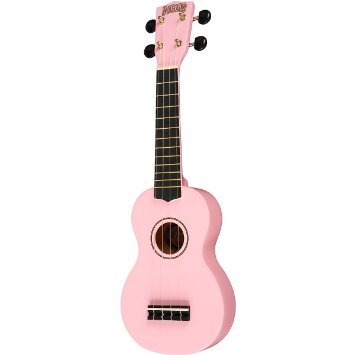
\includegraphics[width=5cm]{../img/ukulele.jpg}
\end{Slide}


% subjekt och predikat -> public static void: https://www.youtube.com/watch?v=1ZPaR_wH-R8


% \begin{Slide}{Koda i Scala}

%   {\footnotesize\it Melodi: McDonalds-låten}

% \begin{verbatim}

%           G         C             G          D
% Det finns stunder i livet som man alltid har kvar

%           G           C               D
% Det finns villkor och uttryck som man spar 

%         A           D             A           E
% Och där dörren står öppen finns gemenskap för fler 

% A      D      E       A
% Koda i Scala; det ger meeeeeeer! 
% \end{verbatim}

% \end{Slide}




\fi

%%!TEX encoding = UTF-8 Unicode
\chapter{Repetition}\label{chapter:W13}
Begrepp som ingår i denna veckas studier:
\begin{itemize}[noitemsep,label={$\square$},leftmargin=*]
\item göra extenta
\item förbereda projektredovisning
\item skapa dokumentation med scaladoc och javadoc\end{itemize}

%!TEX encoding = UTF-8 Unicode
%!TEX root = ../exercises.tex

\ifPreSolution

\Exercise{\ExeWeekTHIRTEEN}\label{exe:W13}
\begin{Goals}
\item Kunna skriva tentamenslika program med papper, penna och snabbreferens som enda hjälpmedel.
\item Förbereda projektredovisningen.
\item Kunna skapa dokumentation med \code{scaladoc} och \code{javadoc}.
\item Kunna skapa jar-filer.
\end{Goals}

% \begin{Preparations}
% \item \StudyTheory{13}
% \end{Preparations}

\else

\ExerciseSolution{\ExeWeekTHIRTEEN}

\fi


\subsection{Förberedelse inför examination}




\WHAT{Gör en extenta.} %%%%%%%%%%%%%%%%%%%%%%%%%%%%%%%%%%%%%%%%%%%%%%%%%%%%%%%%

\QUESTBEGIN

\Task \what~\TODO

\SOLUTION

\TaskSolved \what~\TODO

\QUESTEND




\WHAT{Förbered din projektredovisning.} %%%%%%%%%%%%%%%%%%%%%%%%%%%%%%%%%%%%%%%

\QUESTBEGIN

\Task \what~\TODO

\SOLUTION

\TaskSolved \what~\TODO

\QUESTEND



\WHAT{Skapa dokumentation.} %%%%%%%%%%%%%%%%%%%%%%%%%%%%%%%%%%%%%%%%%%%%%%%%%%%

\QUESTBEGIN

\Task  \what~

\Subtask \TODO kör nedan kommando i terminalen:

\begin{REPL}
> scaladoc paket.scala
> ls
> firefox index.html   # eller öppna index.html i valfri webbläsare
\end{REPL}

Vad händer?

\Subtask Lägg till några fler metoder i något av objekten i filen \code{paket.scala} och lägg även till några dokumentationskommentarer. Kompilera om och kör. Generera om dokumentationen.

\begin{verbatim}
//... ändra i filen paket.scala

/** min paketdokumentationskommentar p2 */
package p2 {
  /** min paketdokumentationskommentar p21 */
  package p21 {
    /** ett hälsningsobjekt */
    object hello {
      /** en hälsningsmetod i p2.p21 */
      def hello = println("Hej paket p2.p21!")

      /** en metod som skriver ut tiden */
      def date = println(new java.util.Date)
    }
  }
}

\end{verbatim}

\begin{REPL}
> gedit paket.scala
> scalac paket.scala
> jar cvf mittpaket.jar gurka
> scala -cp mittpaket.jar
scala> gurka.tomat.banan.p2.p21.hello.date
scala> :q
> scaladoc paket.scala
> firefox index.html
\end{REPL}

\SOLUTION


\TaskSolved \what

\SubtaskSolved  -

\SubtaskSolved  -

\QUESTEND



\WHAT{Repetera övningar och laborationer.} %%%%%%%%%%%%%%%%%%%%%%%%%%%%%%%%%%%%

\QUESTBEGIN

\Task \what~\TODO

\SOLUTION

\TaskSolved \what~\TODO

\QUESTEND

%!TEX encoding = UTF-8 Unicode
%!TEX root = ../compendium2.tex

\Assignment{bank}

\subsection{Fokus}
\begin{itemize}[nosep,label={$\square$},leftmargin=*]
\item Kunna implementera ett helt program efter given specifikation
\item Kunna sätta samman olika delar från olika moduler
\item Förstå hur Java-klasser kan användas i Scala
\item Förstå och bedöma när immutable/mutable såväl som var/val bör användas i större sammanhang
\item Kunna använda sig av kompanjonsobjekt
\item Kunna läsa och skriva till fil
\item Kunna söka i olika datastrukturer på olika sätt
\end{itemize}

\subsection{Bakgrund}

I detta projekt ska du skriva ett program som håller reda på bankkonton och kunder i en bank. Programmet ska utöver att hålla reda på bankens nuvarande tillstånd även föra historik över alla tillståndsändringar. Historiken ska vara så pass detaljerad att det nuvarande tillståndet kan återskapas genom att återuppspela alla ändringar som finns lagrade i historiken.

Programmet ska vara helt textbaserat, man ska alltså interagera med programmet via terminalen där en meny skrivs ut och input görs via tangentbordet.

Du ska skriva större delen av programmet själv, utan någon färdig kod. Programmet ska dock följa de specifikationer som ges i uppgiften, såväl som de objektorienterade principer du lärt dig i kursen.

\subsection{Krav}

Kraven för bankapplikationen återfinns här nedan. För att bli godkänd på denna uppgift måste samtliga krav uppfyllas:

\begin{itemize}
\item Programmet ska ha följande menyval:

\begin{itemize}
\item 1. Hitta konton för en viss kontoinnehavare med angivet ID.
\item 2. Söka efter kunder på (del av) namn.
\item 3. Sätta in pengar på ett konto.
\item 4. Ta ut pengar på ett konto.
\item 5. Överföra pengar mellan två olika konton.
\item 6. Skapa ett nytt konto.
\item 7. Ta bort ett befintligt konto.
\item 8. Skriv ut bankens alla konton, sorterade i bokstavsordning efter innehavare.
\item 9. Återställa banken till tillståndet den hade vid ett givet datum. För enkelhetens skull får du permanent kassera all historik som skapades efter det datum banken återställs till.
\item 10. Avsluta.
\end{itemize}

\item När något av följande sker ska programmet notera det i historiken:
\begin{itemize}
\item Pengar sätts in på ett konto.
\item Pengar tas ut från ett konto.
\item Pengar överförs mellan två konton.
\item Ett konto skapas.
\item Ett konto tas bort.
\end{itemize}
\item Historiken ska sparas både i minnet och i en fil.
\item Då programmet startas ska det läsa in historikfilen för att återskapa tillståndet som banken hade tidigare.
\item Allt som berör användargränssnittet (såsom utskrifter till terminalen och inläsning från terminalen) ska ske i \code{BankApplication} eller hjälpklasser till \code{BankApplication}, inte i någon annan av klasserna som specificeras i uppgiften.
\item Alla metoder och attribut ska ha lämpliga åtkomsträttigheter.
\item Valen av val/var och immutable/mutable måste vara lämpliga.
\item Din indata måste ge samma resultat som i exemplen i bilagan.
\item Rimlig felhantering ska finnas. Det är alltså önskvärt att programmet inte kraschar då man matar in felaktig input, utan istället säger till användaren att input är ogiltlig.
\item Programdesignen ska följa de specifikationer som är angivna nedan.
\item Det räcker med att banken ska kunna hantera heltal, men detta ska göras med klassen \code{BigInt}.
\item Klassen \code{BankAccount} ska generera ett unikt kontonummer för varje konto. Dessa ska återställas om bankens tillstånd återställs till ett tidigare datum, d.v.s. att om en återställning av banken tar bort ett konto så ska dess kontonummer återigen bli tillgängligt.
\end{itemize}

\subsection{Design}
Nedan följer specifikationerna för de olika klasserna bankapplikationen måste innehålla:

\begin{ScalaSpec}{Customer}
/**
 * Describes a customer of a bank with provided name and id.
 */
case class Customer(name: String, id: Long) = {
	override def toString(): String = ???
}
\end{ScalaSpec}


\begin{ScalaSpec}{BankAccount}
/**
 * Creates a new bank account for the customer provided.
 * The account is given a unique account number and initially
 * has a balance of 0 kr.
 */
class BankAccount(val holder: Customer) = {

  /**
   * Deposits the provided amount in this account.
   */
  def deposit(amount: Int): Unit = ???

  /**
   * Returns the balance of this account.
   */
  def getBalance: Int = ???

  /**
   * Withdraws the provided amount from this account,
   * if there is enough money in the account. Returns true
   * if the transaction was successful, otherwise false.
   */
  def withdraw(amount: Int): Boolean = ???
}
\end{ScalaSpec}


\begin{ScalaSpec}{Bank}
/**
 * Creates a new bank with no accounts and no history.
 */
class Bank() = {

 /**
   * Returns a list of every bank account in the bank.
   * The returned list is sorted in alphabetical order based
   * on customer name.
   */
  def getAllAccounts(): Vector[BankAccount] = ???

  /**
   * Returns the account holding the provided account number.
   */
  def findByNumber(accountNbr: Int): Optional[BankAccount] = ???

  /**
   * Returns a list of every account belonging to
   * the customer with the provided id.
   */
  def findAccountsForHolder(id: Long): Vector[BankAccount] = ???

  /**
   * Returns a list of all customers whose names match
   * the provided name pattern.
   */
  def findByName(namePattern: String): Vector[Customer] = ???

 /**
   * Executes an event in the bank.
   * Returns a string describing whether the
   * event was successful or failed.
   */
  def doEvent(event: BankEvent): String = ???

  /**
   * Resets the bank to the state it had at the provided date.
   * Returns a string describing whether the event was
   * successful or failed.
   */
  def returnToState(returnDate: Date): String = ???
}
\end{ScalaSpec}


Till din hjälp innehåller kursens workspace följande färdigskrivna klasser:
\begin{itemize}
\item \code{Date}, en enkel wrapper av \code{Java.time} som du ska använda för att representera tidsstämplar.
\item \code{BankEvent} med tillhörande subtyper, som du ska använda för att representera förändringar av bankens tillstånd.
\end{itemize}


\subsection{Tips}

\begin{itemize}
\item Det enda sättet att förändra tillståndet för en \code{Bank} ska vara (förutom att anropa \code{returnToState}) att anropa \code{doEvent} med en \code{BankEvent} som beskriver tillståndsförändringen. Vid en första anblick kan detta kan verka lite väl bökigt, men när ändringshistoriken ska implementeras kommer det vara till stor hjälp att det finns en \code{BankEvent} som representerar varje ändring.

\item För att skriva till fil på ett enkelt sätt kan man t.ex. använda sig av statiska metoder i klassen \code{Files} som finns tillgänglig i \code{java.nio.file}. För att undvika portabilitetsproblem kan man då använda sig av ett bestämt \code{Charset}, t.ex. \code{UTF_8}, som finns tillgänglig i \code{java.nio.charset.StandardCharsets.UTF_8}.

\item För att läsa ifrån en fil kan man t.ex. använda sig av \code{Source} som finns tillgänglig i \code{scala.io.Source}.

\item Var noggrann med att testerna klarar alla tänkbara fall, och tänk på att fler fall än dem som givits i exempel kan förekomma vid rättning.
\end{itemize}

\subsection{Obligatoriska uppgifter}

\Task Implementera klassen \code{Customer}.

\Task Implementera klassen \code{BankAccount}.

\Task Skapa singelobjektet \code{BankApplication}, som ska innehålla \code{main}-metoden. Det kan vara bra att innan man fortsätter se till att denna skriver ut menyn korrekt och kan ta input från tangentbordet som motsvarar de menyval som finns.

\Task Implementera klassen \code{Bank}.

\Subtask Implementera menyval 6 och 8. Testa noga.

\Subtask Implementera ändringshistoriken. Varje gång \code{doEvent} anropas ska dess \code{BankEvent}-argument läggas till i historiken tillsammans med det nuvarande datumet.

\Subtask Implementera alla andra menyval, förutom menyval 9. Testa de nya menyvalen noga efterhand som du implementerar dem, i synnerhet så att ändringshistoriken fungerar korrekt. Gör de utökningar du anser behövs.

\Task Implementera säkerhetskopiering av historiken.

\Subtask När en \code{BankEvent} läggs till i historiken ska den också skrivas till en historikfil omedelbart. Banken ska ej behöva avslutas för att utskriften ska hamna på fil, om så vore fallet kan information gå förlorad om banken kraschar.

I workspace-katalogen för denna projektuppgift finns en historikfil bifogad. För bekvämlighet finns ett utdrag av denna fil infogad nedanför. Inläsning och utskrift ska ske med dess format:\\~\\
2016 3 7 10 6 N 850127 Fredrik\newline
2016 3 7 10 28 D 1000 16500\newline
2016 3 9 10 52 W 1000 3900\newline
2016 3 9 11 8 N 900318 Casper\newline
2016 3 9 16 28 D 1001 6500\newline
2016 4 1 10 11 W 1001 1900\newline
2016 4 1 11 19 W 1001 2000\newline
2016 4 2 16 33 N 651002 Björn\newline
2016 4 2 16 46 D 1002 25000\newline
2016 4 3 10 11 T 1002 1000 4000\\~\\
Formen är alltså:\\~\\
\textbf{År  Månad  Dag  Timme  Minut  BankEventTag  Parametrar}
\\~\\
De olika klasserna av \code{BankEvent} representeras med följande bokstav:

\begin{itemize}
\item D - \code{Deposit}
\item W - \code{Withdraw}
\item T - \code{Transfer}
\item N - \code{NewAccount}
\item E - \code{DeleteAccount}
\end{itemize}

\Subtask När programmet startar ska det läsa in alla händelser från historikfilen och återuppspela dem en efter en. På så sätt kan bankens tillstånd återställas, fastän vi bara har sparat ändringshistoriken och inte själva tillståndet.

\Task Implementera menyval 9 genom att först nollställa bankens tillstånd och sedan återuppspela allt i historiken som hände före det givna datumet. Resten av historiken bör tas bort permanent, både i minnet och i historikfilen.


\subsection{Frivilliga extrauppgifter}

Gör först klart projektets obligatoriska delar. Därefter kan du, om du vill, utöka ditt program enligt följande.

\Task Skriv en eller flera av klasserna \code{Customer} och \code{BankAccount} i Java istället och använd dig av dessa i din Scala-kod.

\Task	Implementera ett nytt menyalternativ som skriver ut all kontohistorik för en given person. I historiken ska finnas typ av händelse med tillhörande parametrar, dåvarande saldo vid händelsen, såväl som datumet för händelsen.

\subsection{Exempel på körning av programmet}

Nedan visas möjliga exempel på körning av programmet. Data som matas in av användaren är markerad i fetstil.
Ditt program måste inte se identiskt ut, men den övergripande strukturen såväl som resultat av körningen ska vara densamma.
När det första exemplet börjar förutsätts det att banken inte har några konton.

Listan över val, som är markerad i kursiv stil i det första exemplet, är inte utskriven i senare exempel för att spara plats på pappret. Ditt program ska alltid skriva ut listan över val före användaren ska mata in ett val.

% This environment uses minipage to prevent column breaks from occurring in the middle of an example
\newenvironment{exampleblock}
	{\begin{minipage}{\columnwidth}
	 - - - - - - - - - - - - - - - - - - - - - - - - - - -\\}
	{\end{minipage}}

\begin{multicols}{2}
\noindent
\begin{exampleblock}
\textit{
1.   Hitta ett konto för en given kund\\
2.   Sök efter kunder på (del av) namn\\
3.   Sätt in pengar\\
4.   Ta ut pengar\\
5.   Överför pengar mellan konton\\
6.   Skapa nytt konto\\
7.   Radera existerande konto\\
8.   Skriv ut alla konton i banken\\
9.   Återställ banken till ett tidigare datum\\
10.  Avsluta\\
}
Val: \textbf{6}\\
Namn: \textbf{Adam Asson}\\
Id: \textbf{6707071234}\\
Nytt konto skapat med kontonummer: 1000\\
10:03:0 CET 14 / 5 - 2016\\
\end{exampleblock}
\begin{exampleblock}
Val: \textbf{1}\\
Id: \textbf{6707071234}\\
Konto 1000 (Adam Asson, id 6707071234) 0 kr\\
10:04:0 CET 14 / 5 - 2016\\
\end{exampleblock}
\begin{exampleblock}
Val: \textbf{6}\\
Namn: \textbf{Berit Besson}\\
Id: \textbf{8505255678}\\
Nytt konto skapat med kontonummer: 1001\\
10:12:0 CET 14 / 5 - 2016\\
\end{exampleblock}
\begin{exampleblock}
Val: \textbf{2}\\
Namn: \textbf{adam}\\
Adam Asson, id 6707071234\\
10:15:0 CET 14 / 5 - 2016\\
\end{exampleblock}
\begin{exampleblock}
Val: \textbf{8}\\
Konto 1000 (Adam Asson, id 6707071234) 0 kr\\
Konto 1001 (Berit Besson, id 8505255678) 0 kr\\
10:13:0 CET 14 / 5 - 2016\\
\end{exampleblock}
\begin{exampleblock}
Val: \textbf{6}\\
Namn: \textbf{Berit Besson}\\
Id: \textbf{8505255678}\\
Nytt konto skapat med kontonummer: 1002\\
13:56:0 CET 14 / 5 - 2016\\
\end{exampleblock}
\begin{exampleblock}
Val: \textbf{2}\\
Namn: \textbf{erit}\\
Berit Besson, id 8505255678\\
14:01:0 CET 14 / 5 - 2016\\
\end{exampleblock}
\begin{exampleblock}
Val: \textbf{3}\\
Kontonummer: \textbf{1000}\\
Summa: \textbf{5000}\\
Transaktionen lyckades.\\
14:36:0 CET 14 / 5 - 2016\\
\end{exampleblock}
\begin{exampleblock}
Val: \textbf{5}\\
Kontonummer att överföra ifrån: \textbf{1000}\\
Kontonummer att överföra till: \textbf{1001}\\
Summa: \textbf{1000}\\
Transaktionen lyckades.\\
14:37:0 CET 14 / 5 - 2016\\
\end{exampleblock}
\begin{exampleblock}
Val: \textbf{8}\\
Konto 1000 (Adam Asson, id 6707071234) 4000 kr\\
Konto 1001 (Berit Besson, id 8505255678) 1000 kr\\
Konto 1002 (Berit Besson, id 8505255678) 0 kr\\
14:52:0 CET 14 / 5 - 2016\\
\end{exampleblock}
\begin{exampleblock}
Val: \textbf{7}\\
Ange konto att radera: \textbf{1002}\\
Transaktionen lyckades.\\
14:01:0 CET 14 / 5 - 2016\\
\end{exampleblock}
\begin{exampleblock}
Val: \textbf{8}\\
Konto 1000 (Adam Asson, id 6707071234) 4000 kr\\
Konto 1001 (Berit Besson, id 8505255678) 1000 kr\\
14:01:0 CET 14 / 5 - 2016\\
\end{exampleblock}
\begin{exampleblock}
Val: \textbf{9}\\
Vilket datum vill du återställa banken till?\\
År: \textbf{2016}\\
Månad: \textbf{5}\\
Datum (dag): \textbf{9}\\
Timme: \textbf{18}\\
Minut: \textbf{10}\\
Banken återställd.\\
15:00:0 CET 14 / 5 - 2016\\
\end{exampleblock}
\begin{exampleblock}
Val: \textbf{8}\\
Konto 1002 (Björn, id 651002) 25900 kr\\
Konto 1001 (Casper, id 900318) 4600 kr\\
Konto 1003 (Eva, id 950908) 6300 kr\\
Konto 1000 (Fredrik, id 850127) 11800 kr\\
Konto 1004 (Kajsa, id 810722) 17000 kr\\
15:01:0 CET 14 / 5 - 2016\\
\end{exampleblock}
\begin{exampleblock}
Val: \textbf{3}\\
Kontonummer: \textbf{1005}\\
Summa: \textbf{5000}\\
Transaktionen misslyckades. Inget sådant konto hittades.\\
15:06:0 CET 14 / 5 - 2016\\
\end{exampleblock}

\end{multicols}

%!TEX encoding = UTF-8 Unicode
%!TEX root = ../compendium2.tex

\Assignment{tabular}

% \begin{Goals}
% \item Kunna använda mönstermatchning.
% \item Kunna förklara hur \code{Option} användas för att hantera saknde värden.
% \item Kunna använda \code{scala.util.Try} för att hantera undantag.
% %\item Känna till att undantag kan hanteras med \code{try catch}.
% %\item Kunna använda inbyggda sorteringsfunktioner \code{sortBy} och \code{sortWith}.
% %\item Kunna implementera insättningssortering till ny sekvens.
% \item Känna till hur strängar ordnas.
% \item Kunna implementera registrering (frekvensräkning).
% %\item Kunna använda matriser med strängar.
% \end{Goals}

\begin{Preparations}
\item Fyll i denna enkät: \url{https://goo.gl/forms/hC6JK2UQXVpbGECc2}  \\
I enkäten ska du för olika flervalsalternativlistor besvara frågan: \\ \textit{Vilket är ditt favoritalternativ?}
\item Studera den givna koden i \code{src/main/scala/tabular} här: \url{https://github.com/lunduniversity/introprog/tree/master/workspace/w10_tabular}
\end{Preparations}


\subsection{Bakgrund}

Detta projekt innefattar en terminalapplikation som analyserar data i tabeller och ritar statistiska grafer. Indata utgörs av text med \textbf{kolumnseparerade värden}, där varje rad följs av \code{`\n`} och innehåller kolumner som är separerade med ett valfritt s.k. separator-tecken, till exempel \code{','}, \code{'\t'} eller \code{';'}. Din app ska förutsätta att första indataraden innehåller kolumnrubriker.

Du ska använda din app till att analysera svar på enkäter med flervalsfrågor, där varje persons svar finns på en egen rad och varje svarsrad innehåller svarsalternativ i kolumner.
Exempelindata finns i filen \code{favorit.csv} i mappen resources och ser ut som följer. Kolumnseparator i tabellen nedan är \code{","}. Första raden är en rubrikrad som anger kolumnernas respektive rubrik.
\lstinputlisting[basicstyle=\ttfamily\fontsize{10}{12}\selectfont]{../workspace/w10_tabular/src/main/resources/favorit.csv}

\subsection{Krav}\label{tabular:requirements}

\begin{enumerate}[leftmargin=*]
\item Din applikation ska kunna behandla kolumndata i en tabell kallad \code{currentTable}.

\item Den aktuella tabellen ska kunna laddas från disk via filnamn eller från en webbadress som börjar med \code{http}.

\item Din applikation ska acceptera noll, ett eller två argument vid uppstart, där man kan styra ev. textkälla och ev. kolumnseparator.

\item Din applikation ska interagera med användaren genom terminalen och acceptera textkommandot \code{help} som ska ge följande utskrift. Körningen visar utskrift efter uppstart utan argument och resultatet av att användaren skrivit kommandot \code{help} efter prompten \code{"> "}.

\begin{REPLnonum}
Welcome to tabular: an app for analysis of data in tables
Current dir: /home/bjornr/pgk/labs/w10_tabular
No args given. Starting with empty table.
Type 'help' for help on commands and 'quit' to exit app.
> help
Commands:
help                 Print this list of commands
ls                   List files in current directory
load                 Load a file using introprog.Dialog.file
load filename|url    Load a table from <location> using current separator
save                 Save
save filename        Save current table to <filepath>
sep                  Show current column separator
sep c                Change current column separator to char c
show                 Print current table to the console
sort h               Sort current table on heading h
filter h a b c ...   Keep rows where heading h has values a b c ...
pie h                Draw a pie chart of current table's heading h
bar h                Draw a bar chart of current table's heading h
quit, Ctrl+D         Terminate app
\end{REPLnonum}
Följande kommandon är redan implementerade i given kod i modulen \code{Command}: \code{help}, \code{quit}, \code{Ctrl+D} och \code{ls}. Efter listorna nedan med obligatoriska och valfria krav finns en exempelkörning där utdata från olika kommando illustreras.

\item Du ska implementera följande \textbf{obligatoriska} funktioner:
\begin{itemize}[nosep, label={$\square$},]
\item \code{load filename|url} -- laddar \code{currentTable} från fil eller url
\item \code{show} -- visar tabellen i ett inramat rutnät i terminalen (se exempel)
\item \code{sep} -- visar aktuell kolumnseparator
\item \code{sep c} -- ändrar aktuell kolumnseparator till första tecknet i strängen \code{c}
\item \code{sort h} -- sorterar tabellens rader så att kolumnen med rubriken \code{h} är sorterad i bokstavsordning.
\item \code{filter h a b c ...} -- gör så att aktuell tabell bara innehåller de rader där kolumnen med rubriken \code{h} har något av angivna värdena \code{a b c ...}. Värdena ska var minst ett och separeras med blanktecken efter kolumnnamnet \code{h}.
\item \code{load} -- laddar tabell från fil som anges av användaren i en filväljardialog med hjälp av \code{introprog.Dialog.file}
\item \code{save} -- sparar tabell som text till fil som anges av användaren i en filväljardialog med hjälp av \code{introprog.Dialog.file}
\item \code{pie h} -- ritar ett tårtdiagram över antalet förekomster av olika värden i kolumnen med rubriken \code{h} med hjälp av givna koden i \code{Graph.scala}.
\item \code{bar h} -- ritar ett stapeldiagram över antalet förekomster av olika värden i kolumnen med rubriken \code{h} med hjälp av givna koden i \code{Graph.scala}.

\end{itemize}

\item Valfria funktioner:
\begin{itemize}[nosep, label={$\square$},]
\item Implementera funktioner för att göra beräkningar på \emph{numeriska} data i kolumner, t.ex. 
\begin{itemize}
  \item summa för kolumn, \item medelvärde för kolumn, \item standardavvikelse för kolumn.
\end{itemize}
\item Implementera fler statistiska diagram, t.ex. scatterplot i 2 dimensioner för två valda kolumner. \\\url{https://en.wikipedia.org/wiki/Scatter_plot} 
\end{itemize}

\end{enumerate}

\subsection{Design}

Du ska bygga vidare på den delvis färdiga koden i \code{workspace/w10_tabular} enligt denna design:
\begin{itemize}

\item Alla abstraktioner ska ligga i paketet \code{tabular}.

\item Den färdiga modulen \code{Main} hanterar ev. argument och sätter igång användarinteraktionen och gör så att appen inte avbryts om något ej hanterat undantag uppstår.

\item Den påbörjade modulen \code{Command} sköter läs-evaluera-skriv-loopen i programmet. Du ska för varje kommando som du implementerar utöka matchningen i metoden \code{doCommand} med ett mönster som passar med kommandot och ev. argument. Utöka \code{Command} med fler metoder som exekverar resp. kommando som i sin tur tar hjälp av egna eller givna abstraktioner.

\item Den färdiga modulen \code{Graph} ritar diagram i ett \code{PixelWindow}.

\item Den nästan färdiga bastypen \code{Cell} med kompanjonsobjekt och subklasser som representerar en cell i en matris som kan innehålla strängvärden eller numeriska värden. %ingick i uppgift \ref{task:labprep-patterns-tabular} på veckans övning.

\item Den nästan färdiga modulen \code{Table} som representerar en matris med celler. %ingick i uppgift \ref{task:labprep-patterns-tabular} på veckans övning.
\end{itemize}


\subsection{Implementation}

\Task  Bastypen \code{Cell} i koden nedan har två subtyper \code{Str} och \code{Num}.

\begin{CodeSmall}
sealed trait Cell { def value: String }
case class Str(value: String) extends Cell
case class Num(num: BigDecimal) extends Cell { def value = num.toString }
\end{CodeSmall}
\code{BigDecimal} används för att representera decimaltal med bättre precision än vanliga flyttal av typen \code{Double}.

\Subtask Studera dokumentationen för \code{BigDecimal}: \url{https://www.scala-lang.org/api}\\
Vad gör fabriksmetoden \code{def apply(x: String): BigDecimal} (se kompanjonsobj.).


\Subtask Vad är fördelen med att \code{Cell} är förseglad?

\Subtask Kör igång REPL med koden för \code{Cell}-hierarkin tillgänglig på classpath, t.ex. med \code{sbt console}. Vad ger koden nedan för resultat? Ange värde och typ för varje rad.

\begin{REPL}
scala> val xs = Seq[Cell](Str("!"), Num(BigDecimal("100000000.000000001")))
scala> val ys = xs.map(_ match { case Num(n) => Some(n) case _ => None })
scala> val b = ys.flatten.headOption.getOrElse(BigDecimal(0))
\end{REPL}

\Subtask Lägg till ett kompanjonsobjekt enligt nedan. Gör klart den saknade implementationen. Använd \code{Try} och matcha på \code{Success} och \code{Failure}. Testa så att alla metoder i kompanjonsobjektet fungerar.

\Subtask Gör om implementation så att du i stället använder \code{Try} och \code{getOrElse}. Testa så att det fungerar som innan. Vilken implementation är smidigast?
\begin{CodeSmall}
object Cell {
  import scala.util.{Try, Success, Failure}

  /** Ger en Num om BigDecimal(s) lyckas annars en Str. */
  def apply(s: String): Cell =  ???

  def apply(i: Int): Num = Num(BigDecimal(i))

  def empty: Str = Str("")

  def zero: Num = Num(BigDecimal(0))
}
\end{CodeSmall}

\Subtask I given kod och nedan finns en nästan färdig klass för tabelldatahantering. Implementera de saknade delarna enligt beskrivning i dokumentationskommentarerna. Testa så att dina implementationer fungerar och försök förstå hur övriga delar av \code{Table} fungerar.

\scalainputlisting[numbers=left,basicstyle=\ttfamily\fontsize{9}{11.5}\selectfont]{../workspace/w10_tabular/src/main/scala/tabular/Table.scala}

\noindent Tips vid färdigställande av \code{Table}:
\begin{itemize}[leftmargin=*]
  \item Nyckel-värde-tabeller har en metod \code{withDefaultValue} som är smidig om man vill undvika undantag vid uppslagning med nyckel som inte finns och det i stället för undantag är möjligt/lämpligt att erbjuda ett vettigt defaultvärde.
  \item Metoderna \code{getOrElse} och \code{toOption} på en \code{Try} är smidiga när man vill ge resultat som beror av om det är \code{Success} eller \code{Failure} utan att man behöver göra en \code{match}.
\item Skiss på implementation av \code{load} i kompanjonsobjektet:
\begin{CodeSmall}
def load(fileOrUrl: String, separator: Char): Table = {
  val source = fileOrUrl match {
    case /* använd gard och startsWith*/ => scala.io.Source.fromURL(url)
    case path  => scala.io.Source.fromFile(path)
  }
  val lines = try source.getLines.toVector finally source.close
  val rows = ??? // kör split(separator).toVector på alla rader i lines
  Table(rows.head, rows.tail.map(_.map(Cell.apply)), separator)
}
\end{CodeSmall}
En webbadress börjar med \code{http}.
Med \code{try sats1 finally sats2} så kan man garantera att \code{sats2} alltid görs även om \code{sats1} ger undantag. Detta används typiskt för att frigöra resurser som annars förblir allokerade vid undantag. I koden ovan används det för att undvika att filer inte stängs även om något går fel under läsningen.
\end{itemize}

\Task Implementera de obligatoriska och ev. de valfria kraven i avsnitt \ref{tabular:requirements}.

\Task Använd ditt program för att analysera enkätsvar med avseende på t.ex. vilket språk som är populärast på resp. program. Enkätsvar årsvis sedan 2016 finns här \url{http://cs.lth.se/pgk/favorit}

Nedan visas exempelkörning.
\begin{figure}
\begin{REPLnonum}[basicstyle=\color{white}\ttfamily\fontsize{9}{11}\selectfont]
> sep
Current separator: ','
> load favorit.csv
Table loaded with (nCols, nRows) == (17,7)
> sort Program
Current table sorted on column Program
> show
----------------------------------------------------------------------
|Program|Indent|UI      |Lang      |OS        |Browser |DE           |
----------------------------------------------------------------------
|C      |Spaces|Terminal|Javascript|Windows 7 |Chrome  |Notepad++    |
|C      |Spaces|GUI     |Java      |Windows 8 |Firefox |Eclipse      |
|C      |Tabs  |Terminal|C#        |Windows 10|Edge    |Visual Studio|
|D      |Spaces|Terminal|C         |BSD       |Firefox |Emacs        |
|D      |Spaces|GUI     |Java      |macOS     |Safari  |Gedit        |
|D      |Spaces|Terminal|Java      |Windows 8 |Edge    |Eclipse      |
|D      |Spaces|GUI     |C         |Linux     |Firefox |Vim          |
|D      |Tabs  |GUI     |Javascript|macOS     |Chrome  |Emacs        |
|D      |Spaces|GUI     |Python    |Windows 7 |Chrome  |Notepad++    |
|D      |Tabs  |GUI     |C         |Linux     |Chrome  |Gedit        |
|E      |Spaces|Terminal|Java      |Linux     |Chromium|Eclipse      |
|F      |Spaces|Terminal|C         |Linux     |Chrome  |Emacs        |
|F      |Spaces|Terminal|C         |Linux     |Firefox |Vim          |
|I      |Tabs  |Terminal|PHP       |Windows 10|Edge    |Notepad++    |
|I      |Tabs  |Terminal|Python    |Windows 10|Chrome  |Notepad++    |
|K      |Tabs  |GUI     |C#        |Windows 7 |Firefox |Visual Studio|
|Nano   |Tabs  |Terminal|Javascript|macOS     |Safari  |Vim          |
----------------------------------------------------------------------
 (nRows, nCols) == (17,7)

> filter program D C
Filter error.
> filter Program D C
Current table filtered on values Vector(D, C) of column Program
> show
---------------------------------------------------------------------
|Program|Indent|UI      |Lang      |OS        |Browser|DE           |
---------------------------------------------------------------------
|D      |Spaces|Terminal|C         |BSD       |Firefox|Emacs        |
|C      |Spaces|Terminal|Javascript|Windows 7 |Chrome |Notepad++    |
|D      |Spaces|GUI     |Java      |macOS     |Safari |Gedit        |
|C      |Spaces|GUI     |Java      |Windows 8 |Firefox|Eclipse      |
|D      |Spaces|Terminal|Java      |Windows 8 |Edge   |Eclipse      |
|D      |Spaces|GUI     |C         |Linux     |Firefox|Vim          |
|C      |Tabs  |Terminal|C#        |Windows 10|Edge   |Visual Studio|
|D      |Tabs  |GUI     |Javascript|macOS     |Chrome |Emacs        |
|D      |Spaces|GUI     |Python    |Windows 7 |Chrome |Notepad++    |
|D      |Tabs  |GUI     |C         |Linux     |Chrome |Gedit        |
---------------------------------------------------------------------
(nRows, nCols) == (10,7)

> pie Lang
pie chart of heading Lang drawn in another window
> load http://cs.lth.se/pgk/favorit
Table loaded with (nCols, nRows) == (192,8)
> bar Program
bar chart of heading Program drawn in another window
> sep ;
Current separator: ';'
> save data.csv
Table saved to file: data.csv
> ls
/home/bjornr/git/cs/pgk-solutions/solutions-2018/w10_tabular
.classpath favorit-snapshot.csv .settings src project build.sbt data.csv t.csv bin .idea target scp-favorit-snapshot.sh .project favorit.csv lib w10_survey.iml
> quit
Goodbye!

$ cat data.csv  #visa filen och kolla att den har semikolonseparator
\end{REPLnonum}
\end{figure}

Exempel på tårt- och stapeldiagram visas nedan.

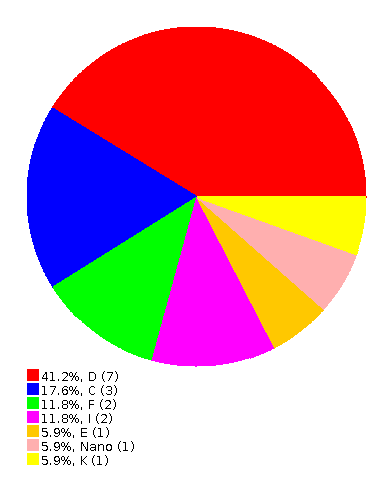
\includegraphics[scale=0.5]{../img/survey/pie.png}

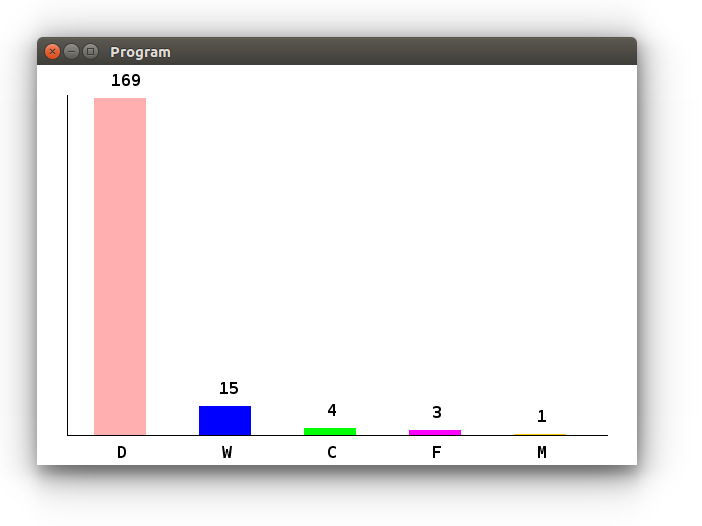
\includegraphics[scale=0.5]{../img/survey/bar.png}

%!TEX encoding = UTF-8 Unicode

%!TEX root = ../compendium2.tex

\Assignment{music}

\begin{Preparations}
\item Testa så att datorn du ska använda på redovisningen kan spela upp ljud med \code{javax.sound.midi} genom att köra igång \code{Main} i den givna koden.
\item Det är bra om du kan ta med hörlurar till datorsalen så att du inte stör andra.
\end{Preparations}

\subsection{Bakgrund}
När man skriver program skapar man ofta modeller av en viss verklig \emph{domän}, som kan vara t.ex. försäkringskassans regelverk eller en fysiksimulering i ett datorspel. För att kunna skapa sådana modeller behöver man ofta skaffa sig  \emph{domänkunskap} genom att noga sätta sig in i vad olika koncept i domänen innebär och hur de är relaterade. Med denna kunskap kan du skapa kod som modellerar domänen, utifrån noga valda förenklingar av den komplexa verkligheten. Förmåga att kunna skapa domänmodeller utgör en viktig grund för konsten att utveckla bra programvarusystem, och du kommer lära dig mer om detta i kommande kurser.

I denna laboration ska du skapa ett program baserat på en förenklad modell av domänen \emph{musik}. Du får färdig kod som modellerar hur toner är uppbyggda, samt hur olika stränginstrument fungerar.
Med denna domänmodell ska du skapa ditt eget musikprogram som använder \emph{ackord} som är uppbyggda av flera toner som spelas tillsammans.

\subsection{Domänmodell}


\subsubsection{Tonhöjd}

En \textbf{ton} \Eng{note} som spelas på ett instrument, t.ex. ett piano eller en gitarr, har en \textbf{tonhöjd} \Eng{pitch} som är relaterad till den specifika  grundfrekvens som tonens ljud har. I vår modell av musikdomänen tillordnar vi olika distinkta tonhöjder ett unikt heltal. En tonhöjd kan då beskrivas av en \code{case class Pitch(nbr: Int)} där vi använder \code{nbr} i intervallet \code{(0 to 127)}. Heltalet \code{60} motsvarar en viss ton, som även har namnet  \code{"C5"}, och som ligger ungefär i mitten av tangentbordet på ett piano.

Inom (västerländsk) musik utgår man från 12 olika \emph{tonklasser} \Eng{pitch classes}.
Dessa tolv tonklasser är ordnade i en sekvens av så kallade \emph{halva tonsteg} och har följande \textbf{tonklassnamn}:
\begin{Code}
  val pitchClassNames: Vector[String] =
    Vector("C","C#","D","D#","E","F","F#","G","G#","A","A#","B")
\end{Code}
Efter tonklassen med namnet \code{B} återkommer tonklassen med namnet \code{C}.
Symbolen \code{#} representerar en höjning ett halvt tonsteg. Tonklassen \code{C#} uttalas \emph{siss} på svenska, och \emph{see sharp} på engelska.\footnote{Man använder även b-förtecknet $\flat$, som uttalas \emph{flat} på engelska, för sänkning av en ton ett halvt tonsteg, men för enkelhetens skull bortser vi i vår modell från detta sätt att namnge toner.}
 Notera att det är ett halvt tonsteg mellan \code{E} och \code{F}, samt mellan \code{B} och \code{C} (det finns därför varken \code{E#} eller \code{B#} i listan med tonklassnamn.\footnote{Varför det är på detta viset kan du läsa mer om på t.ex. Wikipedia, men du kan också nöja dig med att det helt enkelt är så på grund av historiska skäl.})

På ett piano motsvaras de vita tangenterna av tonklassnamen \code{C D E F G A B} och de svarta tangenterna motsvaras av tonklassnamnen \code{C# D# F# G# A#}.

En s.k. \textbf{tonklass} är ett positivt heltal i intervallet \code{0 until 12} som motsvaras av index för tonklassnamnet i \code{pitchClassNames}. En tonhöjd  \code{Pitch(nbr)} tillhör tonklassen \code{nbr % 12}.

Med hjälp av heltalsdivision med 12 får man fram tonhöjdens så kallade \textbf{oktav}, alltså \code{nbr / 12}. Ett piano har normalt toner som spänner över 7 eller 8 oktaver.
En tonhöjd \code{Pitch(nbr)} kan även namnges med en kombination av tonklassnamnet och tonens oktav, t.ex. \code{"C5"}.

Med denna domänbeskrivning kan vi skapa en mer detaljerad modell av konceptet tonhöjd med hjälp av en case-klass och tillhörande kompanjonsobjekt:

\scalainputlisting[basicstyle=\ttfamily\fontsize{10}{13}\selectfont]{../workspace/w10_music/src/main/scala/music/Pitch.scala}

\noindent Kompanjonsobjektet har två fabriksmetoder som kan skapa \code{Pitch}-objekt från en strängrepresentation av en tonhöjd.

\begin{itemize}[noitemsep]
  \item Metoden \code{fromString} omvandlar en sträng till en \code{Option[Pitch]}.

  \item Metoden \code {apply} kastar ett undantag om det inte går att omvandla en sträng till ett \code{Pitch}-objekt.
\end{itemize}

\Task\label{music:exceptions}\Pen Vilka två uttryck i \code{Try}-blocket kan ge undantag? Undersök liknande undantagsuttryck i REPL och skriv ner namnet på undantagen.


\Task Undersök klassen \code{Pitch} i REPL.

\begin{REPL}
> sbt
sbt> console
Welcome to Scala 2.12.6 (Java HotSpot(TM) 64-Bit Server VM, Java 1.8.0_144).

scala> import music._
import music._

scala> Pitch("C#5").nbr
res0: Int = 61

scala> Pitch("C") + 1
res1: music.Pitch = Pitch("C#5")
\end{REPL}


\Subtask\Pen Ge ett exempel på argument till \code{Pitch.apply} som gör att undantag kastas.

\Subtask\Pen Ge ett exempel på argument till \code{Pitch.fromString} som ger \code{None}.

\Subtask\Pen Ge ett exempel på argument till \code{Pitch.+} som gör att undantag kastas.


\Task Ändra i implementationen av \code{fromString} så att du i stället för \code{.toOption} gör en mönstermatchning med \code{match} på \code{Try}-resultaten \code{Success} och \code{Failure} i varsin case-klausul på formen \code{case Sucess(e) => } och \code{case Failure(e: ???) => ???} och returnera lämpligt värde. Ta endast hand om de två förväntade undantagstyperna som du identifierade i uppgift \ref{music:exceptions}. Gör så att alla övriga eventuella undantag kastas genom denna klausul: \code{case Failure(e) => throw e}

\Subtask Testa så att din lösning fungerar i både normalfall och vid felaktigt tonhöjdsnamn.

\Subtask\Pen Undersök vad som händer om du kommenterar bort olika case-klausuler. När ger kompilatorn varning? Varför?

\Subtask\Pen Finns det någon fördel resp. nackdel med att bara fånga vissa undantag?

\subsubsection{Ackord}

Ett ackord består av flera toner som spelas tillsammans. Man kan spela ett ackord på ett stränginstrument genom att slå an en mängd toner samtidigt eller en sekvens av toner i snabb följd. Man väljer att kalla en av tonerna i ackordet (oftast den lägsta/första tonen) för \textbf{grundton} \Eng{root}.

Ett \textbf{intervall} är en tons relativa tonhöjdsavstånd från grundtonen. Ackord har olika namn beroende på vilka intervall som ingår i ackordet. Det finns väldigt många olika ackordnamn, men här begränsar vi oss för enkelhetens skull till fyra olika typer av ackord: \footnote{Om du vill veta mer om ackordnamn läs här: \url{https://en.wikipedia.org/wiki/Chord_(music)}}
\begin{itemize}
  \item dur-ackord, betecknas t.ex. \code{"C"},
  \item moll-ackord, betecknas t.ex. \code{"Cm"}
  \item sju-ackord, betecknas t.ex. \code{"C7"}
  \item maj-sju-ackord som betecknas t.ex. \code{"Cmaj7"}.
\end{itemize}

I case-klassen \code{Chord} nedan finns en metod \code{name} som definerar vilka intervall som ingår i de olika ackordtyperna ovan, utom maj-sju-ackord. Den krångliga modulo-12-omräkningen innan matchningen gör så att intervall i olika oktaver behandlas lika, även för negativa intervall.

\scalainputlisting[basicstyle=\ttfamily\fontsize{10}{13}\selectfont]{../workspace/w10_music/src/main/scala/music/Chord.scala}

\Task

\Subtask Maj-sju-ackord har samma intervall som sju-ackord, förutom att det fjärde intervallet ska vara \code{11} halva tonsteg från grundtonen i stället för \code{10}. Lägg till en case-klausul i \code{Chord.name} så att maj-sju-ackord ges namn som slutar med ändelsen \code{"maj7"}.

\Subtask Testa din kod och kontrollera så att ackordet \code{Chord("D4","F#4","A4","C#5")} får namnet \code{"Dmaj7"}

\begin{REPL}
scala> Chord("D4","F#4","A4","C#5").name()
res2: String = "Dmaj7"
\end{REPL}

\Subtask Vilka fyra toner har ett \code{Cmaj7}-ackord med grundtonen \code{"C5"}?

\subsubsection{Stränginstrument}

Ett stränginstrument, t.ex. ett piano eller en gitarr, kännetecknas av att det kan spela ackord genom att flera strängar kan sättas i svängning så att många toner spelas tillsammans. I vår modell fångar vi denna egenskap med en trait \code{StringInstrument} som har en metod \code{toChordOpt} som ger något ackord om minst en sträng spelas.

Gitarr och ukulele är exempel på stränginstrument som har en greppbräda \Eng{fret board}. Man spelar på ett stränginstrument med greppbräda \Eng{fretted instrument} genom att trycka strängar mot greppbrädan med en hand, samtidigt som man knäpper på strängarna med den andra handen. Olika instanser av dessa  instrument kan skilja sig åt vad gäller antalet strängar och hur dessa strängar är stämda. En normal gitarr har 6 strängar, medan en normal ukulele bara har 4 strängar. Dessa egenskaper modelleras i koden nedan.

Varje sträng har en stämskruv med vilken kan man ändra strängens spänning,  strängens s.k. \textbf{stämning} \Eng{tuning}.  Om man knäpper på alla lösa strängarna på en gitarr med standardstämning spelas tonerna E3, A3, D4, G4, B4, E5, räknat från den tjockaste till den tunnaste strängen.

\scalainputlisting[basicstyle=\ttfamily\fontsize{10}{12.9}\selectfont]{../workspace/w10_music/src/main/scala/music/instruments.scala}

Om man trycker på greppbrädans olika positioner får man olika toner, beroende på vilken position man trycker på. Positionerna på greppbrädan räknas från ett och uppåt. Position \code{0} motsvarar \textbf{lös sträng}, alltså att man slår an en strängen utan att trycka på greppbrädan över denna sträng. En negativ position, tex. \code{-1}, anger att en sträng inte spelas alls; många gitarrackord spelas genom att bara en delmängd av strängarna slås an.
Ett exempel på ett gitarrackord  visas i figur \ref{music:fig:guitar-chord}.

\Task\Pen Studera modellen av stränginstrument ovan och använd REPL för att svara på dessa frågor:

\Subtask Vad är namnet på detta pianoackord om vi väljer att lägsta tonen i ackordet är grundton: \code{Piano(Set(60, 64, 67, 70))}

\Subtask Vad heter tonerna som ingår i ackordet \code{Guitar(3,3,2,0,1,0)}.

\Subtask Vad heter detta ackord om vi väljer ett A som grundton: \code{ Ukulele(0,2,1,2)}


\begin{figure}
  \centering
  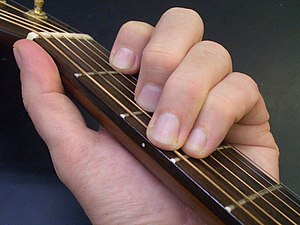
\includegraphics{../img/chords/guitar-C-major-chord.jpg}
  \caption{Ett C-dur-ackord på en gitarr motsvarande \code{Guitar(3,3,2,0,1,0)}.}
  \label{music:fig:guitar-chord}
\end{figure}


\subsubsection{Elektroniska instrument}

Ett elektroniskt instrument syntetiserar ljud med hjälp av analog och/eller digital elektronik, och kallas därför \textbf{synthesizer}, ofta förkortat \emph{synt} \Eng{synth}.

De flesta moderna PC-operativsystem inkluderar mjukvaruimplementerade syntar som följer den så kallade MIDI-standarden. Java-paketet \code{javax.sound.midi} innehåller klasser som kan få en sådan MIDI-synt att spela musik.

MIDI-standarden baseras på en modell av ett pianotangentbord där olika toner kan vara ''på'' eller ''av'' beroende på om en tangent är nedtryckt eller ej. Dessa toners höjd är modellerade på samma sätt som i vår klass \code{Pitch}, där alltså tonhöjden \code{60} motsvarar tonen \code{"C5"}, etc. En tangent kan tryckas ner olika hårt, vilket representeras av ett heltalsvärde i \code{Range(0,128)} kallat \code{velocity}. Ett högt värde ger en stark ton, medan ett litet värde motsvarar en svag (tyst) ton.

En synt som följer MIDI-standarden kan spela upp ljud via 16 olika så kallade \textbf{kanaler} \Eng{channel}, numrerade \code{(0 until 16)},  där varje kanal kan ställas in så att den spelar ett ljud som t.ex. liknar ett visst verkligt instrument, så som piano eller gitarr.

I kursens workspace i paketet \code{music} finns en \code{Synth}-modul som förenklar användningen av Java-paketet \code{javax.sound.midi}. I modulen \code{Synth} finns metoden \code{playBlocking} som kan spela flera toner under en viss tid med hjälp av synten på ditt ljudkort. Exekveringen av ditt program  blockeras tills tonerna spelats klart, därav \emph{''blocking''} i namnet.

Metoden \code{playBlocking} har följande parametrar, default-argument och returtyp:
\footnote{Om du är nyfiken kan du studera implementationen av \code{Synth}-modulen här:
\\\url{https://github.com/lunduniversity/introprog/tree/master/workspace/w10_music}
 Koden blir lättare att förstå om du samtidigt läser api-dokumentationen av paketet \code{javax.sound.midi} och även lära dig mer om MIDI-standarden med hjälp av t.ex. wikipedia.}

\begin{Code}
def playBlocking(
  noteNumbers: Seq[Int] = Seq(60), // en sekvens av tonhöjder
  velocity: Int         = 60,      // hur hårt anslag i Range(0, 128)
  duration: Long        = 300,     // hur länge i millisekunder
  spread:   Long        = 50,      // millisekunder mellan tonerna
  after:    Long        = 0,       // millisekunder innan första tonen
  channel:  Int         = 0        // MIDI-kanal som spelar tonerna
): Unit
\end{Code}


\Task Anropa \code{playBlocking()} i REPL och undersök om din dator kan spela tonen \code{"C5"}. Använd gärna lurar så att du inte stör dina labbkamrater. Prova vad som händer när du ger olika argument till \code{playBlocking}.

\Task Gör klart modulen \code{ChordPlayer} enligt nedan så att metoden \code{play} kan spela ett ackord. Case-klassen \code{Strike} representerar ett ackordanslag.

\scalainputlisting[basicstyle=\ttfamily\fontsize{10}{13}\selectfont]{../workspace/w10_music/src/main/scala/music/ChordPlayer.scala}

\Task Implementera ett singelobjekt med namnet \code{Test} med en \code{main}-metod som med hjälp av din \code{play}-metod från föregående uppgift spelar några olika ackord.

\Task\Checkpoint Inför redovisningen: förbered en förklaring av koden du skrivit, med fokus på hur mönstermatchningen och undantagshanteringen fungerar.


\clearpage

\subsection{Frivilliga extrauppgifter}

\Task Gör en terminalapp som kan spela ackord. I kursens workspace i \code{w10_music} finns en påbörjad terminalapp som du kan bygga vidare på. Den har redan en \code{Main.main}-metod som startar en loop där användaren kan ge kommando \Eng{Command Line Interface, CLI}. Kommandot \code{?} ger hjälp och kommandot \code{:q} avslutar.

\begin{REPL}
*** Welcome to music!
music> ?
?         print help
:q        quit this app
!         play chord TODO
music> !
play chord TODO
music> :q
Goodbye music!
\end{REPL}

Det finns också ett påbörjat kommando \code{!} som är tänkt att spela ett ackord, men som än så länge bara skriver ut ett meddelande. Gör så att användaren med \code{!} kan spela ackord från olika instrument enligt nedan:

\begin{REPL}
music> ! p 60 64 67
Play Piano(Set(60, 64, 67)) Chord(C5,E5,G5)
music> ! g 0 2 2 0 0 0
Play Guitar((0,2,2,0,0,0)) Chord(E3,B3,E4,G4,B4,E5)
\end{REPL}

\noindent\emph{Tips och förslag:} Du kan i stället för \code{scala.io.StdIn.readLine} använda \code{jline} och då får du kommandohistorik med pil upp samt Ctrl+A, Ctrl+E etc. helt automatiskt. Gör helt enkelt så här i \code{Main} i stället för vanliga \code{readLine}:
\begin{CodeSmall}
  val console = new jline.console.ConsoleReader // skapa kommandoläsare
  console.setExpandEvents(false) // stäng av hantering av specialtecken
  def readLine(): String = console.readLine("music> ")
\end{CodeSmall}
Du behöver då lägga till jar-filen\footnote{\url{https://maven2repo.com/jline/jline/2.14.4/jar}} med \code{jline} till ditt bygge. Om du använder sbt kan du göra det enkelt med denna rad i filen \code{build.sbt}:
\begin{CodeSmall}
libraryDependencies += "jline" % "jline" % "2.14.4"
\end{CodeSmall}
Lägg till nedan rader i din \code{build.sbt} så att ditt program körs i en separat JVM, annars blir det konstiga initialiseringsfel av MIDI-systemet om du kör med \code{sbt run}.

\begin{CodeSmall}
fork                := true // https://stackoverflow.com/questions/18676712
connectInput        := true // http://www.scala-sbt.org/1.x/docs/Forking.html
outputStrategy      := Some(StdoutOutput)
\end{CodeSmall}


\Task Bygg vidare på terminalappen \code{music} och implementera fler kommandon. Du kan t.ex. skapa ett kommando som låter användare definierar egna namn på kommandon som sedan enkelt kan köras med hjälp av det definierade namnet.
\begin{REPL}
music> def Em ! g 0 2 2 0 0 0
defined Em: ! g 0 2 2 0 0 0
music> Em
Play Guitar((0,2,2,0,0,0)) Chord(E3,B3,E4,G4,B4,E5)
\end{REPL}


% ...
%
% \vspace{7em}{\TODO OLD TEXT FROM HERE:}
%
%
% \Task ChordDraw
%
% \Subtask Rita upp en greppbräda liknande bilden nedan (kryssen läggs till i kommande uppgifter). Antalet strängar ska variera beroende på instrument.
%
% 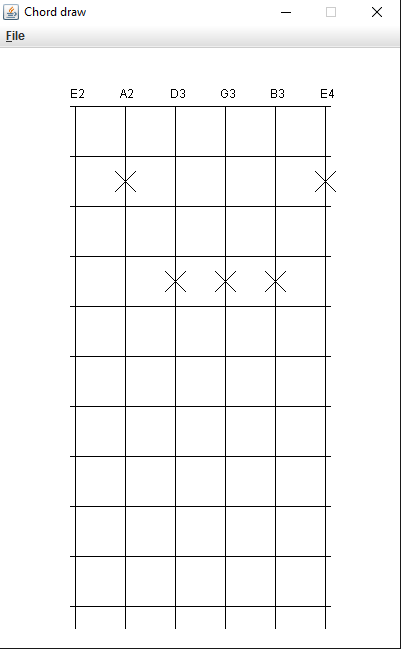
\includegraphics[width=0.5\textwidth]{../img/chords/ChordDraw}
%
% \Subtask Skapa en hjälpmetod \code{cross} som tar in två heltal $x$ och $y$. Metoden ska rita upp ett kryss som är 20x20 pixlar och har sitt centrum i den angivna koordinaten.
%
% \Subtask Rita ut ett kryss där en sträng trycks ner. \textbf{Tänk på att -1 och 0 anger att en sträng inte trycks ner}.
%
% \Subtask Implementera metoden \code{play} som börjar med att vänta på ett event från \code{SimpleWindow}, sedan kollar om eventet är av typen \code{SimpleWindow.MOUSE_EVENT}. Sedan ska man kolla om användaren tryckte på någon sträng (ett intervall på -10 till +10 i förhållande till strängens x-koordinat kan anses vara på strängen). Om användaren tryckt på en sträng ska denna spelas med hjälp av \code{SimpleNotePlayer}. Metoden \code{play} ska köras tills användaren kryssar ner fönstret, vilket motsvarar \code{SimpleWindow.CLOSE_EVENT}.
%
% \Subtask Lägg till menyvalet \code{draw} i \code{textui}. Använd \code{match} för att ta hand om felfallen att inget argument eller fler än ett argument angivits. Argumentet motsvarar ackordets plats i den filtrerade litan. Använd \code{Try} och \code{match} för att ta hand om felet att användaren anger något annat än en siffra. Använd \code{ChordDraw} för att rita upp ackord. \textbf{Kom ihåg att lägga till kommandot i listan med kommandon i \code{doCommand}}

%!TEX encoding = UTF-8 Unicode
%!TEX root = ../compendium.tex

\Assignment{imageprocessing}

\subsection{Bakgrund}

En digital bild består av ett rutnät (en matris) av pixlar. Varje pixel har en färg, och om man har många pixlar flyter de samman för ögat så att de tillsammans skapar en bild.

Det finns olika system för hur man färgsätter de olika pixlarna. T.ex. så används CMYK-systemet (cyan, magenta, gul, svart) vid blandning av färg som ska tryckas på papper eller annat material. På en dator däremot används vanligtvis RGB-systemet. RGB-systemet har tre grundfärger: röd, grön och blå. Mättnaden av varje grundfärg anges av ett heltal som vi i fortsättningen förutsätter ligger i intervallet [0, 255]. 0 anger ”ingen färg” och 255 anger ”maximal färg”. Man kan därmed representera 256 × 256 × 256 = 16 777 216 olika färgnyanser. Man kan också representera gråskalor; det gör man med färger som har samma värde på alla tre grundfärgerna: (0, 0, 0) är helt svart, (255, 255, 255) är helt vitt.


\subsection{Uppgiften}
Du ska skriva ett program där du implementerar olika filter som ska manipulera en given bild på ett flertal olika sätt. Filterklasserna ska ärva från en abstrakt \code{ImageFilter}-klass som är skriven i Java. \code{ImageFilter}-klassen hittar du i cslib.

Följande beskriver \code{ImageFilter}-klassen.

\begin{JavaSpec}{abstract class ImageFilter}
/**
 * Skapar ett filterobjekt med ett givet namn.
 */
protected ImageFilter(String name);

/**
 * Tar reda på filtrets namn.
 */
public String getName();

/**
 * Filtrerar bilden i matrisen inPixels och returnerar
 * resultatet i en ny matris. Utnyttjar eventuellt 
 * värdet av paramValue
 */
public abstract Color[][] apply(Color[][] inPixels,
				 double paramValue);

/**
 * Berättar huruvida ett filter behöver ett parmetervärde eller inte
 * @return true ifall parametervärde behövs, annars false
 */
public abstract boolean needsParameter();

/**
 * Beräknar intensiteten hos alla pixlarna i pixels,
 * returnerar resultatet i en ny matris.
 */
protected short[][] computeIntensity(Color[][] pixels):

/**
 * Faltar punkten p[i][j] med faltningskärnan kernel.
 * 
 * @param p 		matris med talvärden
 * @param i 		radindex får den aktuella punkten
 * @param j 		kolonnindex får den aktuella punkten
 * @param kernel	faltningskärnan, en 3x3-matris
 * @param weight	summan av elementen i kernel
 * @return 		resultatet av faltningen
 */
protected short convolve(short[][] p, int i, int j, 
			short[][] kernel, int weight);
\end{JavaSpec}

Utöver filterklasserna ska du även skapa ett program där du kan välja ett variabelt antal filter och sedan applicera dessa på en bild. För att åstadkomma detta ska du implementera klasserna \code{FilterChooser}, som hanterar val av filter, och \code{FilterList} som representerar vilka filter som ska användas. Klasserna har följande specifikationer:

\begin{ScalaSpec}{FilterList}
class FilterList = ???

/** Adds a filter to the FilterList */
def addFilter(filter: ImageFilter): Unit = ???
  
/** Applies all the filters on the given Image and draws it in SimpleWindow */
def applyFilters(image: Image, sw: SimpleWindow): Unit = ???
\end{ScalaSpec}

\begin{ScalaSpec}{FilterChooser}
/** Creates a FilterChooser with all the available filters */
class FilterChooser(filters: Array[ImageFilter]) = ???
  
/** Shows which filters are available and lets the user choose filters
*   until an escape sequence has been given and returns a FilterList which
*   contain the chosen filters
*   Example: 
*   Tryck på 1 för Blått-filter
*   Tryck på 2 för Kontrast-filter
*   Tryck på 3 för Gauss-filter
*   Tryck på 4 för Sobel-filter
*   Tryck 42 om du inte vill ha fler filter
*/
def chooseFilters(): FilterList = ???
\end{ScalaSpec}

Till din hjälp får du en \code{Image}-klass som representerar en bild samt ett \code{ImageUI} som hjälper dig att ladda in en JPEG bild.

\begin{ScalaSpec}{Image}
class Image(val image: BufferedImage);

/** Returns a matrix of Color-objects that represents an image */
def getColorMatrix: Array[Array[Color]];

/** Updates the image in accordance with the given Color-matrix */
def updateImage(pixels: Array[Array[Color]]): Unit;
\end{ScalaSpec}


\Task \textbf{Blåfilter.} Skriv en klass \code{BlueFilter} som skapar en blå version av bilden. Det vill säga skapa ett filter där varje pixel bara innehåller den blå komponenten. Testa filtret genom att skapa ett \code{ImageProcessing}-object som ska innehålla en \code{main}-metod (\code{ImageProcessing} ska användas och utökas i senare uppgifter). Använd \code{ImageUI} för att välja en bild på följande sätt:
\begin{Code}
val im = new Image(ImageUI.getImage)
\end{Code}
Använd \code{SimpleWindow} samt \code{image} attributet från \code{Image}-objektet för att visa bilden. 

\Task \textbf{inverteringsfilter.} Skriv en klass \code{InvertFilter} som inverterar en bild dvs skapar en ''negativ'' kopia av bilden. Ljusa färger ska alltså bli mörka och mörka färger ska bli ljusa.
Fundera över vad som kan menas med en inverterad eller negativ kopia: de nya RGB-värdena är inte ett dividerat med de gamla värdena (då skulle de nya värdena kunna bli flyttal) och inte de gamla värdena med ombytt tecken (då skulle de nya värdena bli negativa).

\Task \textbf{Gråskalningsfilter.} Skriv en klass \code{GrayScaleFilter} som gör om bilden till en gråskalebild. Använd \code{ImageFilter}s \code{computeIntensity} metod för att bestämma vilken intensitet varje pixel ska ha. Om intensiteten i en pixel till exempel är 105 så ska ett nytt \code{Color}-objekt med värdena (105, 105, 105) skapas.

\Task \textbf{Krypteringsfilter.} Skriv en klass \code{XORCryptFilter} som krypterar bilden med xor-operatorn ˆ. Denna operator gör binär xor mellan bitarna i ett heltal. Exempelvis ger 8 ˆ 127 värdet 119. Om man gör xor igen med 127, alltså 119 ˆ 127, får man tillbaka värdet 8. Varje pixel krypteras genom att använda xor-operatorn med ursprungsvärdena för rött, grönt och blått tillsammans med ett slumpmässigt heltalsvärde som genereras av Scalas Random klass. Använd \code{paramValue} för att ge \code{Random}-objektet ett seed. På så sätt kan du återskapa bilden genom att applicera krypteringsfiltret igen, med samma \code{paramValue}, på den numera krypterade bilden.

\Task \textbf{Gaussfiltrer.} Gaussfiltrering är ett exempel på så kallad faltningsfiltrering. Filtreringen bygger på att man modifierar varje bildpunkt genom att titta på punkten och omgivande punkter. 

För detta utnyttjar man en så kallad faltningskärna K som är en liten kvadratisk heltalsmatris. Man placerar K över varje element i intensitetsmatrisen och multiplicerar varje element i K med motsvarande element i intensitetsmatrisen. Man summerar produkterna och dividerar summan med summan av elementen i K för att få det nya värdet på intensiteten i punkten. Divisionen med summan gör man för att de nya intensiteterna ska hamna i rätt intervall.

Exempel:

\begin{minipage}{5cm}
\begin{displaymath}
\mathit{intensity} = \left(
\begin{array}{ccccc}
5 & 4 & 2 & 8 & \ldots \\
4 & 3 & 4 & 9 & \ldots \\
9 & 8 & 7 & 7 & \ldots \\
8 & 6 & 6 & 5 & \ldots \\
\vdots & \vdots & \vdots & \vdots & \ddots
\end{array}
\right)
\end{displaymath}
\end{minipage}\hspace{2cm}
\begin{minipage}{5cm}
\begin{displaymath}
K = \left(
\begin{array}{ccc}
0 & 1 & 0 \\
1 & 4 & 1 \\
0 & 1 & 0
\end{array}
\right)
\end{displaymath}
\end{minipage}

Här är summan av elementen i $K$ $1+1+4+1+1 = 8$. För att räkna ut det nya värdet på intensiteten i punkten med index \code{(1)(1)} (det nuvarande värdet är 3) beräknar man:

\begin{displaymath}
\mathit{newintensity} = \frac{0 \cdot 5 + 1 \cdot 4 + 0 \cdot 2 + 1 \cdot 4 + 4 \cdot 3 + 1 \cdot 4 + 0 \cdot 9 + 1 \cdot 8 + 0 \cdot 7}{8} = \frac{32}{8} = 4
\end{displaymath}


Man fortsätter med att flytta K ett steg åt höger och beräknar på motsvarande sätt ett nytt värde för elementet med index \code{(1)(2)} (där det nuvarande värdet är 4 och det nya värdet blir 5). Därefter gör man på samma sätt för alla element utom för ”ramen” dvs elementen i matrisens ytterkanter.

Skriv en klass \code{GaussFilter}som implementerar denna algoritm. Varje färg ska behandlas separat. Gör på följande sätt:
\begin{enumerate}
	\item Bilda tre short-matriser och lagra pixlarnas red-, green- och blue-komponenter i matriserna.
	\item Utför faltningen av de tre komponenterna för varje element och lagra ett nytt \code{Color}-objekt i \code{outPixels} för varje punkt.
	\item Elementen i ramen behandlas inte, men i \code{outPixels} måste också dessa element få värden. Enklast är att flytta över dessa element oförändrade från \code{inPixels} till \code{outPixels}. Man kan också sätta dem till \code{Color.WHITE}, men då kommer den filtrerade bilden att se något mindre ut.
\end{enumerate}

Använd \code{ImageFilter}s \code{convolve}-metod för att utföra faltningen. Metoden behöver en faltningsmatris, \code{kernel}, som input och ska anropas med red-, green- och blue-matrisen. Faltningsmatrisen kan vara ett attribut i klassen och ska ha följande utseende:

\begin{displaymath}
\begin{pmatrix}
  0 & 1 & 0 \\
  1 & 4 & 1 \\
  0 & 1 & 0 \\
\end{pmatrix}
\end{displaymath}

Det kan vara intressant att prova med andra värden än 4 i mitten av faltningsmatrisen. Med värdet 0 får man en större utjämning eftersom man då inte alls tar hänsyn till den aktuella pixelns värde. Mata in detta värde i Parameter-rutan. 

Anmärkning: det kan ibland vara svårt att se någon skillnad mellan den filtrerade bilden och originalbilden. Om man vill ha en riktigt suddig bild så måste man använda en större matris som faltningskärna.


\Task  \textbf{Sobelfiltrer.} Sobelfiltrering är, precis som Gaussfiltrering, en typ av faltningsfiltrering. Med Sobelfiltrering får man dock motsatt effekt i jämförelse med Gaussfiltrering, dvs man förstärker konturer i en bild. I princip deriverar man bilden i x- och y-led och sammanställer resultatet.

\begin{figure}[H]
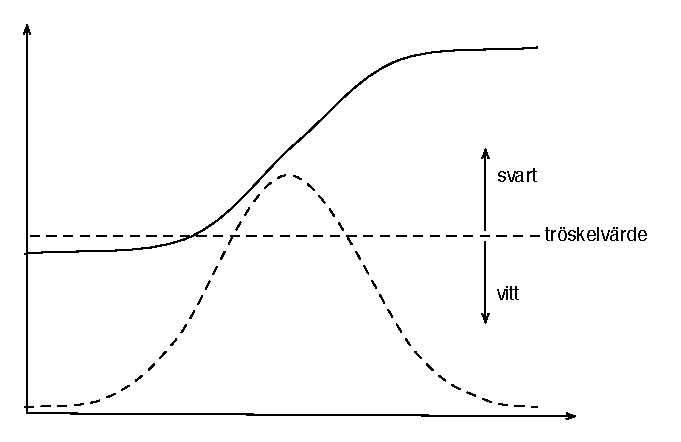
\includegraphics[width=\textwidth]{../img/w13-assignment-imageprocessing/derivatabild2.pdf}
\caption { En funktion (heldragen linje) och dess derivata (streckad linje).}
\label{fig:derivatabild}
\end{figure}

I figur~\ref{fig:derivatabild} visas en funktion $f$ (heldragen linje) och funktionens derivata $f'$ (streckad linje). Vi ser att där funktionen gör ett ''hopp'' så får derivatan ett stort värde. Om funktionen representerar intensiteten hos pixlarna längs en linje i x-led eller y-led så motsvarar ''hoppen'' en kontur i bilden. Om man sedan bestämmer sig för att pixlar där derivatans värde överstiger ett visst tröskelvärde ska vara svarta och andra pixlar vita så får man en bild med bara konturer. 

Nu är ju intensiteten hos pixlarna inte en kontinuerlig funktion som man kan derivera enligt vanliga matematiska regler. Men man kan approximera derivatan, till exempel med följande formel:

\begin{displaymath}
f'(x) \approx \frac{f(x+h) - f(x-h)}{2h}
\end{displaymath}

(Om man här låter $h$ gå mot noll så får man definitionen av derivatan.) Uttryckt i Scala och matrisen \code{intensity} så får man:

\begin{Code}
val derivative = (intensity(i)(j+1) - intensity(i)(j-1)) / 2
\end{Code}

Allt detta kan man uttrycka med hjälp av faltning. 

\begin{enumerate} 
	\item Beräkna intensitetsmatrisen med metoden \code{computeIntensity}.
	\item Falta varje punkt i intensitetsmatrisen med två kärnor:
$$
X\_SOBEL =
\begin{pmatrix}
  -1 & 0 & 1 \\
  -2 & 0 & 2 \\
  -1 & 0 & 1 \\
\end{pmatrix}
Y\_SOBEL =
\begin{pmatrix}
  -1 & -2 & -1 \\
  0 & 0 & 0 \\
  1 & 2 & 1 \\
\end{pmatrix}
$$
	Använd metoden \code{convolve} med vikten 1. Koefficienterna i matrisen $X\_SOBEL$ uttrycker derivering i x-led, i $Y\_SOBEL$ faltning i y-led. För att förklara varför koefficienterna ibland är 1 och ibland 2 måste man studera den bakomliggande teorin noggrant, men det gör vi inte här.
	\item Om resultaten av faltningen i en punkt betecknas med \code{sx} och \code{sy} så får man en indikator på närvaron av en kontur med \code{math.abs(sx) + math.abs(sy)}. Absolutbelopp behöver man eftersom man har negativa koefficienter i faltningsmatriserna. 
	\item  Sätt pixeln till svart om indikatorn är större än tröskelvärdet, till vit annars. Tröskelvärdet bestäms av \code{paramValue}. 
\end{enumerate}

Skriv en klass \code{SobelFilter} som implementerar denna algoritm.

\begin{figure}[H]
\begin{center}
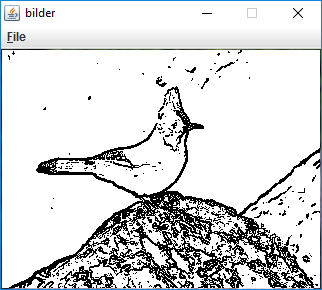
\includegraphics[scale=0.8]{../img/w13-assignment-imageprocessing/sobeljay.png}
\caption { Exempel på en bild där ett Sobelfilter applicerats med ett parametervärde på 150.}
\label{fig:sobel}
\end{center}
\end{figure}


\Task Implementera \code{FilterList} enligt specifikationerna ovan.

\Task Implementera \code{FilterChooser} enligt specifikationerna ovan.

\Task Knyt ihop allt i \code{ImageProcessing}-objektet som du skapade innan. Utskrifterna ska se ut på följande sätt:

{\setlength{\parindent}{0cm}

 Välj en av följande bilder genom att mata in en siffra\newline

0. boy.jpg\newline
1. car.jpg\newline
2. duck.jpg\newline
3. facade.jpg\newline
4. jay.jpg\newline
5. moon.jpg\newline
6. obidos.jpg\newline
7. sgrada.jpg\newline
8. shuttle.jpg\newline
Ditt val: 1\newline
Bild car.jpg laddad\newline
Tryck på 0 för Vanligt-filter\newline
Tryck på 1 för Blått-filter\newline
Tryck på 2 för Krypterat-filter\newline
Tryck på 3 för Inverterat-filter\newline
Tryck på 4 för Grått-filter\newline
Tryck på 5 för Kontrast-filter\newline
Tryck på 6 för Gauss-filter\newline
Tryck på 7 för Sobel-filter\newline
Tryck 42 om du inte vill använda fler filter\newline
Välj ett filter 1\newline
Välj ett filter 42\newline
Välja ny bild? (y/n) n\newline
}

Tänk på att användaren kan mata in otillåtna värden. Detta ska hanteras på lämpligt sätt.

\subsection{Frivilliga extrauppgifter}

\Task \textbf{Kontrastfilter.} Om man applicerar kontrastfiltrering på en färgbild så kommer bilden att konverteras till en gråskalebild. (Man kan naturligtvis förbättra kontrasten i en färgbild och få en färgbild som resultat. Då behandlar man de tre färgkanalerna var för sig.) Många bilder lider av alltför låg kontrast. Det beror på att bilden inte utnyttjar hela det tillgängliga området 0–255 för intensiteten. Man får en bild med bättre kontrast om man ''töjer ut'' intervallet enligt följande formel (lineär interpolation):

\begin{Code}
val newIntensity = 255 * (intensity - 45) / (225 - 45)
\end{Code}

Som synes kommer en punkt med intensiteten 45 att få den nya intensiteten 0 och en punkt med intensiteten 225 att få den nya intensiteten 255. Mellanliggande punkter sprids ut jämnt över intervallet \code{[0, 255]}. För punkter med en intensitet mindre än 45 sätter man den nya intensiteten till 0, för punkter med en intensitet större än 225 sätter man den nya intensiteten till 255. Vi kallar intervallet där de flesta pixlarna finns för \code{[lowCut, highCut]}. De punkter som har intensitet mindre än \code{lowCut} sätter man till 0, de som har intensitet större än \code{highCut} sätter man till 255. För de övriga punkterna interpolerar man med formeln ovan (45 ersätts med \code{lowCut}, 225 med \code{highCut}).

Det återstår nu att hitta lämpliga värden på \code{lowCut} och \code{highCut}. Detta är inte något som kan göras helt automatiskt, eftersom värdena beror på intensitetsfördelningen hos bildpunkterna. Man börjar med att beräkna bildens intensitetshistogram, dvs hur många punkter i bilden som har intensiteten 0, hur många som har intensiteten 1, . . . , till och med 255.

I de flesta bildbehandlingsprogram kan man sedan titta på histogrammet och interaktivt bestämma värdena på \code{lowCut} och \code{highCut}. Så ska vi dock inte göra här. I stället bestämmer vi oss för ett procenttal \code{cutOff} (som bestäms av \code{paramValue}) och beräknar \code{lowCut} så att \code{cutOff} procent av punkterna i bilden har en intensitet som är mindre än \code{lowCut} och \code{highCut} så att \code{cutOff} procent av punkterna har en intensitet som är större än \code{highCut}.

Exempel: antag att en bild innehåller 100 000 pixlar och att \code{cutOff} är 1.5. Beräkna bildens intensitetshistogram i en vektor
\begin{Code} 
val histogram = Array[Int](256)
\end{Code}

Beräkna \code{lowCut} så att \code{histogram(0)} + ... + \code{histogram(lowCut)} = 0.015 * 100000 (så nära det går att komma, det blir troligen inte exakt likhet). Beräkna \code{highCut} på liknande sätt.

Sammanfattning av algoritmen:
\begin{enumerate}
	\item Beräkna intensiteten hos alla punkterna i bilden, lagra dem i en \code{short}-matris. Använd den färdigskrivna metoden \code{computeIntensity}.
	\item Beräkna bildens intensitetshistogram.
	\item Parametervärdet \code{paramValue} är det värde som ska användas som \code{cutOff}.
	\item Beräkna \code{lowCut} och \code{highCut} enligt ovan.
	\item Beräkna den nya intensiteten för varje pixel enligt interpolationsformeln och lagra de nya pixlarna i \code{outPixels}.
\end{enumerate}
Skriv en klass \code{ContrastFilter} som implementerar algoritmen. I katalogen \emph{images} kan bilden \emph{moon.jpg} vara lämpliga att testa, eftersom den har låg kontrast. Anmärkning: om \code{cutOff} sätts = 0 så får man samma resultat av denna filtrering som man får av \code{GrayScaleFilter}. Detta kan man se genom att studera interpolationsformeln.


%!TEX encoding = UTF-8 Unicode

%!TEX root = ../compendium1.tex

%!TEX encoding = UTF-8 Unicode
\chapter{Muntlig examen}\label{chapter:W14}


%%!TEX encoding = UTF-8 Unicode
\chapter{Muntlig examen}\label{chapter:W14}

%!TEX encoding = UTF-8 Unicode
%!TEX root = ../exercises.tex

\ifPreSolution

\Exercise{\ExeWeekFOURTEEN}\label{exe:W14}

\begin{Goals}
\item Känna till vad en tråd är och kunna förklara begreppet jämlöpande exekvering.
\item Känna till vad metoderna \code{run} och \code{start} gör i klassen \code{Thread}.
\item Kunna skapa och starta en tråd med överskuggad \code{run}-metod.
\item Kunna skapa ett enkelt program som från två trådar tävlar om att uppdatera en variabel och förklara varför beteendet kan bli oförutsägbart.
\item Kunna använda en \code{Future} för att köra igång flera parallella beräkningar.
\item Kunna registrera en callback på en \code{Future} med metoden \code{onComplete}.
%\item Känna till att webbsidor beskrivs av HTML-kod och kunna skapa en minimal webbsida.
%\item Kunna ladda ner en webbsida med \code{scala.io.Source.fromURL}.
\end{Goals}

% \begin{Preparations}
% \item \StudyTheory{14}
% \end{Preparations}

\else

\ExerciseSolution{\ExeWeekFOURTEEN}

\fi


\subsection{Frivilliga extrauppgifter}



\WHAT{Trådar.}

\QUESTBEGIN

\Task  \what~   Klassen \code{java.lang.Thread} används för att skapa  \textbf{trådar} med jämlöpande exekvering \Eng{concurrent execution}. På så sätt kan man få olika koddelar att köra samtidigt.

Klassen \code{Thread} definierar en tom \code{run}-metod. Vill man att tråden ska göra något vettigt får man överskugga \code{run} med det man vill ska göras.

En tråd körs igång med metoden \code{start} och då anropas automatiskt \code{run}-metoden och tråden exekverar koden i \code{run} jämlöpande med övriga trådar. Om man anropar \code{run} direkt blir det \emph{inte} jämlöpande exekvering.

\Subtask Skapa en tråd som gör något som tar lite tid och kör med \code{run} resp. \code{start}.
\begin{REPL}
def zzz = { print("zzzzzz"); Thread.sleep(5000); println(" VAKEN!")}
zzz
val t2 = new Thread{ override def run = zzz }
t2.run
t2.run; println("Gomorron!")
t2.start; println("Gomorron!")
t2.start
\end{REPL}

\Subtask Vad händer om man anropar \code{start} mer än en gång på samma tråd?

\Subtask Skapa två trådar med överskuggade \code{run}-metoder och kör igång dem samtidigt enligt nedan. Vilken ordning skrivs hälsningarna ut efter rad 3 resp. rad 4 nedan? Förklara vad som händer.
\begin{REPL}
val g = new Thread{ override def run = for (i <- 1 to 100) print("Gurka ") }
val t = new Thread{ override def run = for (i <- 1 to 100) print("Tomat ") }
g.run; t.run
g.start; t.start
\end{REPL}

\Subtask Använd \code{Thread.sleep} enligt nedan. Är beteendet helt förutsägbart (deterministiskt)? Förklara vad som händer. Du kan (om du kör Linux) avbryta REPL med Ctrl+C%
\footnote{\href{http://stackoverflow.com/questions/6248884/can-i-stop-the-execution-of-an-infinite-loop-in-scala-repl}{stackoverflow.com/questions/6248884/can-i-stop-the-execution-of-an-infinite-loop-in-scala-repl}}.
\begin{REPL}
def ibland(block: => Unit) = new Thread {
  override def run = while(true) { block; Thread.sleep(600) }
}.start
ibland(print("zzz ")); ibland(print("snark ")); ibland(println("hej!"))
\end{REPL}


\SOLUTION


\TaskSolved \what
     %%%TODO number  1 %%%starts with: \emph{Trådar.}  %%%

\SubtaskSolved   -

\SubtaskSolved  \code {java.lang.IllegalThreadStateException}. Det går inte att starta en tråd mer än en gång. Tråden kan därför inte startas om när den redan har exekverats.

\SubtaskSolved   När \code {start} anropas exekveras koden i \code{run} parallellt. Därför skrivs \code{Gurka} och \code{Tomat} ut omlöpande. Om istället \code{run} anropas direkt blir det inte jämnlöpande exekvering och \code{Gurka} skrivs ut 100 gånger, sedan skrivs \code{Tomat} ut 100 gånger.

\SubtaskSolved   \code{Thread.sleep} pausar inte tråden i exakt den tiden som angets. Alltså kommer det skrivas ut \code{zzz snark hej!} i de flesta fall, men det är inte garanterat.



\QUESTEND






\WHAT{Jämlöpande variabeluppdatering.}

\QUESTBEGIN

\Task \label{task:racecondition} \what~   Skriv klasserna \code{Bank} och \code{Kund} i en editor och klistra sedan in koden i REPL.

\begin{Code}
class Bank {
  private var saldo = 0;
  def visaSaldo: Unit = println("saldo: " + saldo)
  def sättIn: Unit = { saldo += 1 }
  def taUt: Unit   = { saldo -= 1 }
}

class Kund(bank: Bank) {
  def slösaSpara = {bank.taUt; Thread.sleep(1); bank.sättIn}
}
\end{Code}

\Subtask Använd funktionen \code{ibland} från föregående uppgift och kör nedan rader i REPL. Resultatet av jämlöpande variabeluppdatering blir här heltokigt och leder till mycket upprörda bankkunder och -ägare. Förklara vad som händer.

\begin{REPL}
val bank = new Bank
bank.visaSaldo
bank.sättIn
bank.visaSaldo
bank.taUt
bank.visaSaldo

val bamse = new Kund(bank)
val skutt = new Kund(bank)

bamse.slösaSpara
skutt.slösaSpara
bank.visaSaldo

def ofta(block: => Unit) = new Thread {
  override def run = while(true) { block; Thread.sleep(1) }
}.start

ofta(bamse.slösaSpara); ofta(skutt.slösaSpara)

ibland(bank.visaSaldo)
\end{REPL}


\SOLUTION


\TaskSolved \what
     %%%TODO number  2 %%%starts with: \emph{Jämlöpande variabeluppdat%%%

\SubtaskSolved  I \code{slösaSpara} hämtas saldot, ändras och placeras tillbaka i minnet -  fördröjs -  upprepas. Om \code{bamse} blir klar med att ladda, ändra och lagra innan skutt gör detsamma med den muterbara variablen hade det inte varit perfekt. Problemet ligger i  när en tråd laddar och innan den kan lagra det förändrade värdet laddar den andra tråden samma värde. Bara en av dessa trådar vinner racet och får lagra sitt ändrade tal. \code{skutt} och \code{bamse} blir alltså upprörda för att inte alla dess uttag och insättningar registreras.


\QUESTEND






\WHAT{Trådsäkra \code{AtomicInteger}.}

\QUESTBEGIN

\Task  \what~  Det finns stöd i JVM för att åstadkomma uppdateringar som inte kan avbrytas av andra trådar under pågånde minnesskrivning. En operation som inte kan avbrytas kallas \textbf{atomär} \Eng{atomic}. Studera dokumentationen för \code{AtomicInteger}\footnote{\href{https://docs.oracle.com/javase/8/docs/api/java/util/concurrent/atomic/AtomicInteger.html}{docs.oracle.com/javase/8/docs/api/java/util/concurrent/atomic/AtomicInteger.html}} och prova nedan kod. Förklara vad som händer.

Använd funktionerna \code{ofta} och \code{ibland} från tidigare uppgifter.
\begin{Code}
class SäkerBank {
  import java.util.concurrent.atomic.AtomicInteger
  private var saldo = new AtomicInteger
  def visaSaldo: Unit = println(s"saldo: ${saldo.get}")
  def sättIn: Unit = { saldo.incrementAndGet }
  def taUt: Unit   = { saldo.decrementAndGet }
}

class SäkerKund(bank: SäkerBank) {
  def slösaSpara = {bank.taUt; Thread.sleep(1); bank.sättIn}
}
\end{Code}
\begin{REPL}
val säkerBank = new SäkerBank
val farmor = new SäkerKund(säkerBank)
val vargen = new SäkerKund(säkerBank)

ofta(farmor.slösaSpara); ofta(vargen.slösaSpara)

ibland(säkerBank.visaSaldo)
\end{REPL}





\SOLUTION


\TaskSolved \what
     %%%TODO number  3 %%%starts with: \emph{Jämlöpande exekvering med%%%

Nu är \code{farmor} garanterad att kunna ladda saldot, ta ut pengar/ändra och lagra innan \code{vargen} kan överskriva resultatet. I \code{slösaSpara} pausas tråden i en millisekund så \code{vargen} kan fortfarande ta ut pengar innan \code{farmor} hinner sätta in pengar igen. Dock kommer alla uttag och insättningar registreras eftersom operationerna är atomära.


\QUESTEND






\WHAT{Jämlöpande exekvering med \code{scala.concurrent.Future}.}

\QUESTBEGIN

\Task \label{task:future} \what~   Att skapa och hålla reda på trådar kan bli ganska omständligt och knepigt att få rätt på.
Med hjälp av \code{scala.concurrent.Future} kan man på ett enklare sätta skapa jämlöpande exekvering.

\begin{Background}
Med en \code{Future} skapas jämlöpande exekvering som ''under huven'' använder ett ramverk som heter Akka\footnote{\url{http://akka.io/}}, skrivet i Scala och Java. Akka erbjuder automatisk  multitrådning med s.k. trådpooler och möjliggör avancerad parallellprogrammering på en hög  abstraktionsnivå, där man själv slipper skapa instanser av klassen \code{Thread}. I stället kan man helt enkelt placera sin kod inramad med \code|Future{ "körs parallellt" }| efter att man importerat det som behövs.
\end{Background}

\Subtask För att skapa jämlöpande exekvering med \code{Future} behöver man först göra import enligt nedan; då skapas ett exekveringssammanhang med trådpooler redo för användning. Starta om REPL och studera felmeddelandet efter rad 1 nedan. Importera därefter enligt nedan. Vad har \code{f} för typ?
\begin{REPL}
scala> concurrent.Future { Thread.sleep(1000); println("En sekund senare!") }
scala> import scala.concurrent._
scala> import ExecutionContext.Implicits.global
scala> val f = Future { Thread.sleep(1000); println("En sekund senare!") }
\end{REPL}

\Subtask Skapa en procedur \code{printLater} enligt nedan som skriver ut argumentet efter slumpmässig tid. Förklara vad som händer nedan.
\begin{REPL}
scala> def printLater(a: Any): Unit =
         Future { Thread.sleep((math.random * 10000).toInt); print(a + " ") }
scala> (1 to 42).foreach(i => printLater(i)); println("alla är igång!")
\end{REPL}

\Subtask Skapa enligt nedan en \code{Future} som räknar ut hur många siffror det är i ett väldigt stort tal. Med \code{onComplete} kan man ange vad som ska göras när den tunga beräkningen är färdig; detta kallas att ''registrera en callback''. Vilken returtyp har \code{big}? Hur många siffror har det stora talet? Vad har \code{r} för typ? Justera argumentet till \code{big} om du inte orkar vänta på resultatet...

\begin{REPL}
scala> BigInt(10).pow(100)
scala> BigInt(10).pow(100).toString.size
scala> def big(n: Int) = Future { BigInt(n).pow(n).toString.size }
scala> big(1234567).onComplete{r => println(r + " siffror") }
\end{REPL}

\Subtask Den stora vinsten med \code{Future} är att man kan köra vidare under tiden, varför anropet av \code{Future} kallas \textbf{icke-blockerande} \Eng{non-blocking}. Det händer ibland att man ändå vill blockera exekveringen i väntan på ett resultat. Man kan då använda objektet \code{scala.concurrent.Await} och dess metod \code{result} enligt nedan. Använd \code{big} från föregående uppgift och gör en blockerande väntan på resultatet enligt nedan. Vad händer? Vad händer om du väntar för kort tid?

\begin{REPL}
scala> import scala.concurrent.duration._
scala> Await.result(big(1234567), 20.seconds)
\end{REPL}



\SOLUTION


\TaskSolved \what
     %%%TODO number  4 %%%starts with: TODO  %%%%%%%%%%%%%%%%%%%\Advan%%%

\SubtaskSolved  error: Cannot find an implicit ExecutionContext. Future behöver en ExecutionContext för att kunna köras. \code{f} är av typen Future[Unit].

\SubtaskSolved  Funktionen \code{printLater} har en Future, vilket innebär att när både \code{printLater} och \code{println} anropas i foreach-loopen exekveras dom jämnlöpande. Eftersom det tar längre tid att starta upp en Future för datorn är \code{println} snabbare och skriver ut att alla är igång först. Sedan skrivs siffrorna från 1 - 42 ut med oregelbundna mellanrum eftersom tråden pausas olika länge.

\SubtaskSolved  \code{big} är en Future[Int]. Det stora talet har 7 520 383 siffror. \code{r} är av typen Try[Int] (se dokumentationen för Future om du är osäker)

\SubtaskSolved  Eftersom exekveringen blockas tills den har fått ett resultat går det inte att fortsätta skriva i REPL medan uträkningen pågår. Väntar man för kort tid får man ett TimeOutException och uträkningen avbryts.


\QUESTEND






\WHAT{Använda \code{Future} för att göra flera saker samtidigt.}

\QUESTBEGIN

\Task  \what~
I denna uppgift ska du ladda ner webbsidor parallellt med hjälp av \code{Future}, så att en nedladdning kan avslutas under tiden en annan dröjer.

\Subtask Koden för en minimal webbsida ser ut som nedan. Du kan beskåda sidan här: \url{http://fileadmin.cs.lth.se/pgk/mini.html} eller skriva in nedan kod i en fil som heter något som slutar på \texttt{.html} och öppna filen i din webbläsare.

\begin{verbatim}
<!DOCTYPE html>
<html>
<body>
HELLO WORLD!
</body>
</html>
\end{verbatim}

\Subtask För att simulera slöa webbservrar kan man ladda ner en sida via sajten \texttt{http://deelay.me/}. Ladda ner ovan sida med 2 sekunders fördröjning:\\
\url{http://deelay.me/2000/http://fileadmin.cs.lth.se/pgk/mini.html}

\Subtask Man kan ladda ner webbsidor med \code{scala.io.Source}. Vad händer nedan? Försök, med ledning av hur \code{delay} beräknas, uppskatta hur lång tid du måste vänta i medeltal, i bästa fall, respektive värsta fall, innan du kan se första webbsidan i vektorn \code{laddningar} nedan?

\begin{REPL}
scala> def ladda(url: String) = scala.io.Source.fromURL(url).getLines.toVector
scala> def slöladda(url: String) = {
         val delay = (math.random * 1000 + 2000).toInt
         val delaySite = s"http://deelay.me/$delay/"
         ladda(delaySite+url)
      }
scala> ladda("http://fileadmin.cs.lth.se/pgk/mini.html")
scala> def seg = slöladda("http://fileadmin.cs.lth.se/pgk/mini.html")
scala> val laddningar = Vector.fill(10)(seg)
scala> laddningar(0)
\end{REPL}

\Subtask Innan vi kan köra igång en \code{Future} så måste vi, som visats i uppgift \ref{task:future} importera den underliggande exekveringsmiljön som är redo att parallelisera ditt program i trådar utan att du själv måste skapa dem. Vad händer nedan?
\begin{REPL}
scala> import scala.concurrent._
scala> import ExecutionContext.Implicits.global
scala> val f = Future{ seg }
scala> f   // kolla om den är klar annars prova igen senare
scala> f
\end{REPL}

\Subtask Ladda indata utan att blockera \Eng{non-blocking input}. Förklara vad som händer nedan.
\begin{REPL}
scala> val nonblock = Future{ Vector.fill(10)(seg) }
scala> nonblock   // kolla igen senare om ej klar
scala> nonblock
\end{REPL}

\Subtask Ladda indata separat i olika parallella trådar. Förklara vad som händer nedan. Kör uttrycket på rad 3 nedan upprepade gånger i snabb följd efter varandra med pil-upp+Enter i REPL.
\begin{REPL}
scala> val para = Vector.fill(10)(Future{ seg })
scala> para
scala> para.map(_.isCompleted)
scala> para.map(_.isCompleted) // studera hur de blir färdiga en efter en
scala> para(0)
\end{REPL}

\Subtask Registrera en callback med metoden \code{onComplete}. Förklara vad som händer nedan.

\begin{REPL}
scala> val action = Vector.fill(10)(Future{ seg })
scala> action(0).onComplete(xs => println(s"ready:$xs"))
scala> // vänta tills laddning på plats 0 är klar
\end{REPL}

\Subtask Registrera en callback för felhantering i händelse av undantag med metoden \code{onFailure}. Förklara vad som händer nedan.
\begin{REPL}
scala> def lycka  = { Thread.sleep(3000); println(":)") }
scala> def olycka = { Thread.sleep(3000); 42 / 0; lycka }
scala> Future{ lycka  }.onFailure{ case e => println(s":( $e") }
scala> Future{ olycka }.onFailure{ case e => println(s":( $e") }
\end{REPL}



\SOLUTION


\TaskSolved \what
     %%%TODO number  5 %%%starts with: Sök upp och studera dokumentati%%%

\SubtaskSolved  -

\SubtaskSolved  -

\SubtaskSolved  Varje sida fördröjs med mellan 2 upp till 3 sekunder (2000-3000 millisekunder). Så i medeltal tar det 2.5 sekunder för varje sida att laddas. Vektorn måste fyllas innan exekveringen kan fortsätta. Därför laddas alla 10 stycken sidor in innan man kan se första websidan. Det tar därför i medeltal 2.5 x 10 = 25 sekunder.

\SubtaskSolved  \code{f} ger en Vektor fylld med strängar där varje element ges av en rad på hemsidan. Då \code{f} körs i bakgrunden kan programmet fortlöpa medan innehållet räknas ut. Du kan därför skriva \code{f} i REPL:n men det är inte säkert att proccessen är klar och det slutgilltiga resultatet visas.

\SubtaskSolved  Samma som ovan, förutom att det blir en vektor där varje element är i sig en vektor med strängar.

\SubtaskSolved  Laddar in datan parallelt så nedladdingen sker samtidigt, men det går olika snabbt pga metoden seg.

\SubtaskSolved  Eftersom datan laddas i parallella trådar utan blockering blir dom inte klara i ordning, utan i den ordningen tråden körs klart. Till slut blir alla klara och resultatet visar en vektor med \code{true} värden.

\SubtaskSolved  Metoden \code{lycka} är väldefinerad och kastar därför inga undantag. Den skriver alltid ut \code{:)}. Metoden \code{olycka} är inte väldefinerad då division med 0 ger \code{java.lang.ArithmeticException}. Detta fångas upp vid callbacken och det skrivs ut \code{:(} samt det specifierade undantaget.

\ExtraTasks %%%%%%%%%%%%


\QUESTEND






\WHAT{}

\QUESTBEGIN

\Task  \what~ Räkna ut stora primtal parallellt genom att använda nedan funktioner. Implementera \code{isPrime} enligt pseudokod från den engelska wikipediasidan om primtalstest\footnote{\href{https://en.wikipedia.org/wiki/Primality_test}{en.wikipedia.org/wiki/Primality\_test}} med den s.k. ''naiva algoritmen''.  Räkna ut 10 st slumpvisa primtal med 16 siffror vardera. Gör beräkningarna parallellt med hjälp av \code{Future}.

\begin{Code}
def isPrime(n: BigInt): Boolean = ???

def nextPrime(start: BigInt): BigInt = {
  var i = start
  while (!isPrime(i)) { i += 1 }
  i
}

def randomBigInt(nDigits: Int): BigInt = {
   def rndChar = ('0' + (math.random * 10).toInt).toChar
   val str = Array.fill(nDigits)(rndChar).mkString
   BigInt(str)
}
\end{Code}

\SOLUTION


\TaskSolved \what
  %%%TODO number  6 %%%

\begin{Code}
def isPrime(n: BigInt): Boolean = n match {
  case _ if (n <= 1) => false
  case _ if (n <= 3) => true
  case _ if n % 2 == 0 || n % 3 == 0 => false
  case _ =>
    var i = BigInt(5)
    while (i * i < n) {
      if (n % i == 0 || n % (i + 2) == 0) false
      i += 6
    }
    true
}

import scala.concurrent._
import ExecutionContext.Implicits.global

val primes = Vector.fill(10)(Future{nextPrime(randomBigInt(16))})
primes.foreach(_.onSuccess{case i => println(i)})
\end{Code}


\QUESTEND






\WHAT{Svara på teorifrågor.}

\QUESTBEGIN

\Task  \what~\Pen

\Subtask Vad är en tråd?

\Subtask Hur skapar man en tråd med klassen \code{Thread}?

\Subtask Hur startar man en tråd?

\Subtask Vilka problem kan man råka ut för om man uppdaterar samma resurs i flera olika trådar?

\Subtask Vad innbär det att kod är \emph{trådsäker}?

\Subtask Nämn några fördelar med att använda Future jämfört med att använda trådar direkt.


\SOLUTION


\TaskSolved \what
 %%%TODO number  7 %%%

\SubtaskSolved  Stackoverflow ger följande förklaring:

A thread is an independent set of values for the processor registers (for a single core). Since this includes the Instruction Pointer (aka Program Counter), it controls what executes in what order. It also includes the Stack Pointer, which had better point to a unique area of memory for each thread or else they will interfere with each other.

\SubtaskSolved

\begin{Code}
val thread = new Thread(new Runnable{
	def run(){println(''Det här är en tråd'')}
})
\end{Code}

\SubtaskSolved  \code{thread.start}

\SubtaskSolved  Det kan bli kapplöpning(race conditions) om vilken tråds resurser blir sparade. Vilket leder till att de andra trådarnas ändringar blir ignorerade.

\SubtaskSolved  Trådsäkerhet innebär att flera trådar kan köras parallellt utan felaktigheter i resultatet. Exempelvis får man vara väldigt försiktig om man vill ha en muterbar variabel som alla trådar ska ändra samtidigt.

\SubtaskSolved  Till exempel slipper man skapa instanser av klassen Thread eftersom man kan placera koden i en Future istället. Den löser även mycket under huven för kodaren.


\QUESTEND






\WHAT{Klasser med atomär uppdatering.}

\QUESTBEGIN

\Task  \what~ Läs om och testa klasserna AtomicBoolean, AtomicDouble och AtomicReference för atomär uppdatering i paketet \code{java.util.concurrent.atomic}. Använd några av dessa tillsammans med \code{scala.concurrent.Future}.


\SOLUTION

\TaskSolved --

\QUESTEND





\WHAT{Skapa din egen multitrådade webbserver.}

\QUESTBEGIN

\Task  \what~

\Subtask Skriv in\footnote{Eller ladda ner här: \href{https://github.com/lunduniversity/introprog/blob/master/compendium/examples/simple-web-server/webserver.scala}{github.com/lunduniversity/introprog/blob/master/compendium/examples/simple-web-server/webserver.scala}} nedan kod i en editor och spara i en fil med namn \texttt{webserver.scala} och kompilera och kör med \texttt{scala webserver.start} och beskriv vad som händer när du med din webbläsare surfar till adressen: \\ \url{http://localhost:8089/abbasillen}

\scalainputlisting[numbers=left,basicstyle=\ttfamily\fontsize{11}{12}\selectfont]{examples/simple-web-server/webserver.scala}

\Subtask Du ska nu skapa en webbserver som gör något lite mer intressant. Den ska svara med det 13:e Fibonacci-talet\footnote{\href{https://sv.wikipedia.org/wiki/Fibonaccital}{https://sv.wikipedia.org/wiki/Fibonaccital}} om du surfar till \url{http://localhost:8089/fib/13}.
Spara din webbserver från föregående deluppgift under det nya namnet \texttt{fibserver.scala} och använd koden nedan och lägg till och ändra så att din server kan svara med Fibonaccital. Vi börjar med att räkna ut Fibonaccital i funktionen \code{compute.fib} nedan på ett onödigt processorkrävande sätt med exponentiell tidskomplexitet så att webbservern verkligen får jobba, för att i senare deluppgifter implementera \code{compute.fib} med linjär tidskomplexitet och därmed undvika onödig planetuppvärmning.
\begin{CodeSmall}
  object compute {
    def fib(n: BigInt): BigInt = {
      if (n < 0) 0 else
      if (n == 1 || n == 2) 1
      else fib(n - 1) + fib(n -2)
    }
  }

  def fibResponse(num: String) = Try { num.toInt } match {
    case Success(n) => html.page(s"fib($n) == " + compute.fib(n))
    case Failure(e) => html.page(s"FEL $e: skriv heltal, inte $num")
  }

  def errorResponse(uri:String) = html.page("FATTAR NOLL: " + uri)

  def handleRequest(cmd: String, uri: String, socket: Socket): Unit = {
    val os = socket.getOutputStream
    val parts = uri.split('/').drop(1) // skip initial slash
    val response: String = (parts.head, parts.tail) match {
      case (head, Array(num)) => fibResponse(num)
      case _                  => errorResponse(uri)
    }
    os.write(html.header(response.size).getBytes("UTF-8"))
    os.write(response.getBytes("UTF-8"))
    os.close
    socket.close
  }
\end{CodeSmall}
Kör i terminalen med \texttt{scala fibserver.start} och beskriv vad som händer i din webbläsare när du surfar till servern.


%%%\textbf{KOD TILL FACIT:}
%%%\scalainputlisting[numbers=left,basicstyle=\ttfamily\fontsize{11}{12}\selectfont]{examples/simple-web-server/fibserver.scala}


\Subtask Surfa efter flera stora Fibonacci-tal samtidigt i olika flikar i din browser. Hur märks det att servern bara kör i en enda tråd?

\Subtask Gör din server multitrådad med hjälp av den nya server-loopen nedan.

\begin{CodeSmall}
import scala.concurrent._
import ExecutionContext.Implicits.global

  def serverLoop(server: ServerSocket): Unit = {
    println(s"http://localhost:${server.getLocalPort}/hej")
		while (true) {
  		Try {
  		  var socket = server.accept  // blocks thread until connect
	  	  val scan = new Scanner(socket.getInputStream, "UTF-8")
		    val (cmd, uri) = (scan.next, scan.next)
			  println(s"Request: $cmd $uri")
		    Future { handleRequest(cmd, uri, socket) }.onFailure {
		      case e => println(s"Reqest failed: $e")
		    }
		  }.recover{ case e: Throwable => s"Connection failed: $e" }
		}
  }
\end{CodeSmall}

\Subtask Surfa efter flera stora Fibonacci-tal samtidigt i olika flikar i din browser. Hur märks det att servern är multitrådad?


\Subtask Det är onödigt att räkna ut samma Fibonacci-tal flera gånger. Med hjälp av en cache i form av en föränderlig \code{Map} kan du spara undan redan uträknade värden. Det funkar dock inte med en vanlig \code{scala.collection.mutable.Map} i vår multitrådade webbserver, eftersom den inte är \textbf{trådsäker} \Eng{thread-safe}. Med trådosäkra föränderliga datastrukturer blir det samma besvärliga beteende som i uppgift \ref{task:racecondition}.

Du ska i stället använda \code{java.util.concurrent.ConcurrentHashMap}. Sök upp  dokumentationen för \code{ConcurrentHashMap} och försök förstå koden nedan. Hur fungerar metoderna \code{containsKey}, \code{put} och \code{get}?
\begin{Code}
object compute {
  import java.util.concurrent.ConcurrentHashMap
  val memcache = new ConcurrentHashMap[BigInt, BigInt]

  def fib(n: BigInt): BigInt =
    if (memcache.containsKey(n)) {
      println("CACHE HIT!!! no need to compute: " + n)
      memcache.get(n)
    } else {
      println("cache miss :( must compute fib:  " + n)
      val f = fastFib(n)
      memcache.put(n, f)
      f
    }

  private def fastFib(n: BigInt): BigInt = {
    if (n < 0) 0 else
    if (n == 1 || n == 2) 1
    else fib(n - 1) + fib(n -2)
  }
}
\end{Code}

\Subtask Använd ovan \code{fib}-objekt i en ny version av din webserver. Spara den i en ny kodfil med namnet \texttt{fibserver-memcached.scala}. Undersök hur snabbt det går med stora Fibonaccital med den nya varianten. Hur stora tal kan du räkna ut? Kan servern fortsätta efter överflödad stack? Förklara varför.

\Subtask Nu när vi kan få väldigt stora Fibonacci-tal kan det vara användbart att stoppa in radbrytningar på webbsidan. Html-taggen \texttt{</br>} ger en radbrytning.
\begin{Code}
  def insertBreak(s: String, n: Int = 80): String = {
    if (s.size < n) s
    else s.take(n) + "</br>" + insertBreak(s.drop(n),n)
  }
\end{Code}
Använd den rekursiva funktionen ovan för att pilla in radbrytningstaggar på var $n$:te position i långa strängar. Testa hur det ser ut på webbsidan med ovan funktion när din server svarar med väldigt stora tal.

\Subtask Vi ska nu använda det större heap-minnet i stället för stack-minnet och därmed inte begränsas av stackens max-storlek. Skriv om \code{fastFib} så att den använder en \code{while}-sats i stället för ett rekursivt anrop. Denna uppgift är ganska klurig, men om du kör fast kan du snegla i lösningarna i Appendix för inspiration.

Hur stora tal klarar din server nu? Vad händer med servern när minnet tar slut? Hur kan du skydda servern så att den inte kan hänga sig?

\SOLUTION


\TaskSolved \what
 %%%TODO number  9 %%%

\SubtaskSolved  \code{abbasillen} skrivs ut baklänges till \code{nellisabba}.

\SubtaskSolved

\SubtaskSolved

\SubtaskSolved

\SubtaskSolved

\SubtaskSolved

\SubtaskSolved

\SubtaskSolved

\SubtaskSolved

Lösningsförslag:
\scalainputlisting[numbers=left,basicstyle=\ttfamily\fontsize{11}{12}\selectfont]{examples/simple-web-server/fibserver-threaded-memcached-while.scala}


\QUESTEND






\WHAT{}

\QUESTBEGIN

\Task  \what~ Utöka din server med fler beräkningsintensiva funktioner. Exempelvis primtalsberäkningar eller beräkningar av valfritt antal decimaler av $\pi$ eller $e$. Utnyttja gärna det du lärt dig i  matematiken om summor och serieutvecklingar.

\SOLUTION


\TaskSolved \what
 %%%TODO number  10 %%%

---


\QUESTEND






\WHAT{}

\QUESTBEGIN

\Task  \what~ Läs mer om \code{Future} och jämlöpande exekvering i Scala här:\\
\href{http://alvinalexander.com/scala/future-example-scala-cookbook-oncomplete-callback}{alvinalexander.com/scala/future-example-scala-cookbook-oncomplete-callback}

\SOLUTION


\TaskSolved \what
 %%%TODO number  11 %%%

---


\QUESTEND






\WHAT{}

\QUESTBEGIN

\Task  \what~ Läs mer om jämlöpande exekvering och multitrådade program i Java här: \href{http://www.tutorialspoint.com/java/java_multithreading.htm}{www.tutorialspoint.com/java/java\_multithreading.htm}  \\
\noindent När man skriver program med jämlöpande exekvering finns det många fallgropar; det kan bli kapplöpning \Eng{race conditions} om gemensamma resurser och dödläge \Eng{deadlock} där inget händer för att trådar väntar på varandra. Mer om detta i senare kurser.


\SOLUTION


\TaskSolved \what
 %%%TODO number  12 %%%

---


\QUESTEND






\WHAT{Studera dokumentationen i \code{scala.concurrent}.}

\QUESTBEGIN

\Task  \what~\Pen

\Subtask Studera dokumentationen för \code{scala.concurrent.Future}\footnote{\href{http://www.scala-lang.org/files/archive/api/current/\#scala.concurrent.Future}{http://www.scala-lang.org/files/archive/api/current/\#scala.concurrent.Future}}. Hur samverkar \code{Future} med \code{Try} och \code{Option}? Vilka vanliga samlingsmetoder känner du igen?

\Subtask Studera dokumentationen för \code{scala.concurrent.duration.Duration}\footnote{\href{http://www.scala-lang.org/api/current/\#scala.concurrent.duration.Duration}{www.scala-lang.org/api/current/\#scala.concurrent.duration.Duration}}. Vilka tidsenheter kan användas?

\Subtask Vid import av \code{scala.concurrent.duration._ } dekoreras de numeriska klasserna med metoder för att skapa instanser av klassen \code{Duration}. Detta möjligörs med hjälp av klassen \code{scala.concurrent.duration.DurationConversions}. Studera dess dokumentation och testa att i REPL skapa några tidsperioder med metoderna på \code{Int}.



\SOLUTION


\TaskSolved \what
 %%%TODO number  13 %%%

\SubtaskSolved

\SubtaskSolved

\SubtaskSolved


\QUESTEND






\WHAT{}

\QUESTBEGIN

\Task  \what~ Fördjupa dig inom webbteknologi.

\Subtask Lär dig om HTML, CSS och JavaScript här: \url{https://developer.mozilla.org/en-US/docs/Learn}

\Subtask Lär dig om Scala.JS här: \url{http://www.scala-js.org/}\SOLUTION


\TaskSolved \what
 %%%TODO number  14 %%%

\SubtaskSolved  ---

\SubtaskSolved  ---

\SubtaskSolved  ---

\SubtaskSolved  ---
\QUESTEND

%!TEX encoding = UTF-8 Unicode
%%% EMPTY


\part{Appendix}
\appendix

%\setcounter{chapter}{8} %next after 8 is I in \Alph
%\setcounter{chapter}{3} %next after 3 is D in \Alph
%!TEX encoding = UTF-8 Unicode
%!TEX root = ../compendium2.tex

\chapter{Kojo}\label{appendix:kojo}

\section{Vad är Kojo?}

Kojo%
\footnote{\href{https://en.wikipedia.org/wiki/Kojo_(programming_language)}{en.wikipedia.org/wiki/Kojo\_(programming\_language)}}
 är en integrerad utvecklingsmiljö för Scala som är speciellt anpassad för programmeringsundervisning i grundskolan. Kojo används i LTH:s Science Center Vattenhallen för utbildning av grundskolelärare i programmering och vid skolbesök och annan besöksverksamhet, i vilken lärare och studenter vid LTH arbetar som handledare. 
 
 Kojo är öppen källkod och utvecklingsgemenskapen leds av Lalit Pant från Indien. I Kojo finns även lättillgängliga bibliotek som gör tröskeln lägre att programmera rörlig grafik och enkla spel.

Under kursens första laboration använder vi grafikbiblioteket i Kojo för att illustrera grundläggande begrepp, så som sekvens, alternativ, repetition och abstraktion.  


\begin{figure}[H]
\centering
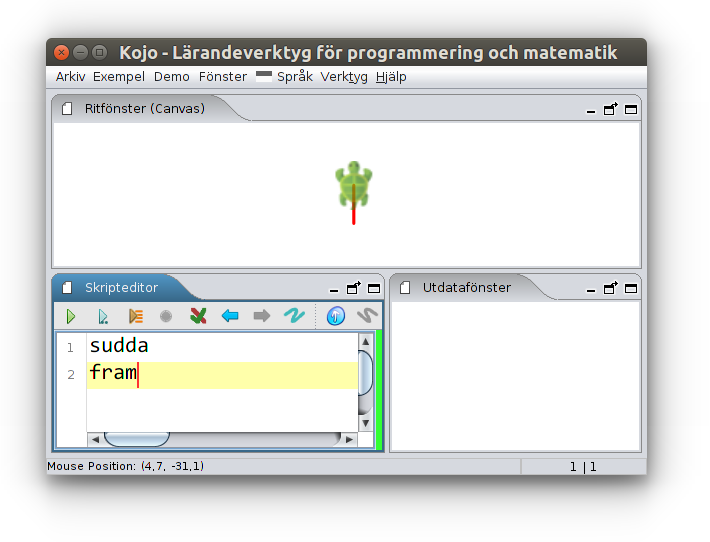
\includegraphics[width=0.8\textwidth]{../img/kojo/kojo.png}
\caption{Den nybörjarvänliga utvecklingsmiljön Kojo för Scala på svenska.}
\label{fig:appendix:ide:kojo}
\end{figure}

\section{Använda grafikbiblioteket i Kojo}\label{appendix:ide:kojo:install}

Kojo bygger på den beprövade pedagogiska idén med sköldpaddsgrafik \Eng{turtle graphics}\footnote{\url{https://en.wikipedia.org/wiki/Turtle_graphics}}, där du skriver program som styr en sköldpadda med en penna under magen. När sköldpaddan rör sig bildas ett streck av valfri färg på skärmen. Beroende på hur du bestämmer att sköldpaddan ska röra sig och vilken färg du bestämmer att pennan ska ha, kan du skapa olika intressanta bilder och samtidigt lära dig om programmeringens grunder.

Under kursens första laboration ska du använda grafikbiblioteket i Kojo tillsammans med editorn VS \code{code} och \code{scala-cli} i terminalen (se appendix \ref{appendix:terminal} och \ref{appendix:compile}). Ladda ner filen \texttt{kojo.scala} från \url{https://cs.lth.se/pgk/kojolib} och spara i en ny katalog med hjälp av din webbläsare, eller via dessa kommandon:

\begin{REPLnonum}
> mkdir w01-kojo
> cd w01-kojo
> curl -o kojolib.scala -sL https://cs.lth.se/pgk/kojolib
\end{REPLnonum}

Nu kan du starta Scala REPL och rita med Kojo så här:

\begin{REPLnonum}
> scala-cli repl .
Welcome to Scala 3.1.2 (17.0.2, Java OpenJDK 64-Bit Server VM).
Type in expressions for evaluation. Or try :help.
                                                                                                                               
scala> fram; höger; fram; vänster

\end{REPLnonum}

Du kan starta VS \code{code} i aktuellt bibliotek så här:
\begin{REPLnonum}
> code .
\end{REPLnonum}

Skriv nedan progam i VS \code{code} och spara det i samma katalog som den tidigare nedladdade filen, under ett nytt valfritt filnamn, t.ex. \code{rita.scala}:

\begin{Code}
@main def rita =
  fram; höger
  fram; vänster
\end{Code}

Kör ditt fristående program med:
\begin{REPLnonum}
> scala-cli run .
\end{REPLnonum}

Du ska nu få upp ett fönster som heter Kojo Canvas med en sköldpadda som ritat två streck. När du stänger fönstret så avslutas programmet. Prova fler sköldpaddsfunktioner enligt tabell \ref{table:kojo:functions}.

I stället för att ladda ned filen \code{kojolib.scala} så kan du placera dess innehåll på lämpligt ställe i ditt program enligt nedan. Observera att raden som börjar med \code{//> using lib} ska vara en enda lång rad utan radbrytningar. Raden med \code{export} gör Kojos kommandon tillgängliga utan prefix:
\begin{CodeSmall}[breaklines=true]
//> using scala "3"
//> using lib "net.kogics:kojo-lib:0.1.1,url=https://github.com/lunduniversity/introprog/releases/download/kojo-lib-0.1.1/kojo-lib-0.1.1.jar"

export net.kogics.kojo.Swedish.*, padda.*, CanvasAPI.*, TurtleAPI.*
\end{CodeSmall}


\noindent Scala-koden för den svenska paddans api finns här: \\
%\href{https://github.com/litan/kojo/blob/master/src/main/scala/net/kogics/kojo/lite/i18n/svInit.scala}{github.com/litan/kojo/blob/master/src/main/scala/net/kogics/kojo/lite/i18n/svInit.scala} \\
\href{https://github.com/litan/kojo-lib/blob/main/src/main/scala/net/kogics/kojo/i18n/Swedish.scala}{github.com/litan/kojo-lib/blob/main/src/main/scala/net/kogics/kojo/i18n/Swedish.scala}


%Kojo kräver (numera) \emph{inte} att \texttt{java} finns på din dator utan kommer med en egen JVM. 
%Eftersom du behöver tillgång till JDK i kursen, är det lika bra att installera hela JDK direkt (och inte bara JRE, så som beskrivs å länken ovan); se vidare hur du gör detta i avsnitt \ref{appendix:compile:install-jdk}.
%\href{http://www.kogics.net/kojo-download}{www.kogics.net/kojo-download}


{\small\renewcommand{\arraystretch}{1.4}
\begin{longtable}{@{}p{0.42\textwidth} p{0.55\textwidth}}

\caption{Ett urval av funktioner i Kojo. Se även \href{http://lth.se/programmera}{lth.se/programmera}}\label{table:kojo:functions}\\

\emph{Svenska/Engelska} & \emph{Vad händer?}  \\ \hline
\code|sudda| \newline \code|clear| & Ritfönstret suddas \\
\code|fram| \newline \code|forward()| & Paddan går framåt 25 steg. \\
\code|fram(100)| \newline \code|forward(100)| & Paddan går framåt 100 steg. \\
\code|höger| \newline \code|right(90)| & Paddan vrider sig 90 grader åt höger. \\
\code|höger(45)| \newline \code|right(45)| & Paddan vrider sig 45 grader åt höger. \\
\code|vänster| \newline \code|left(90)| & Paddan vrider sig 90 grader åt vänster. \\
\code|vänster(45)| \newline \code|left(45)| & Paddan vrider sig 45 grader åt vänster. \\
\code|hoppa| \newline \code|hop| & Paddan hoppar 25 steg utan att rita. \\
\code|hoppa(100)| \newline \code|hop(100)| & Paddan hoppar 100 steg utan att rita. \\
\code|hoppaTill(100, 200)| \newline \code|jumpTo(100, 200)| & Paddan hoppar till läget (100, 200) utan att rita. \\
\code|gåTill(100, 200)| \newline \code|moveTo(100, 200)| & Paddan vrider sig och går till läget (100, 200). \\
\code|hem| \newline \code|home| & Paddan går tillbaka till utgångsläget (0, 0). \\
\code|öster| \newline \code|setHeading(0)| & Paddan vrider sig så att nosen pekar åt höger. \\
\code|väster| \newline \code|setHeading(180)| & Paddan vrider sig så att nosen pekar åt vänster. \\
\code|norr| \newline \code|setHeading(90)| & Paddan vrider sig så att nosen pekar uppåt. \\
\code|söder| \newline \code|setHeading(-90)  | & Paddan vrider sig så att nosen pekar neråt. \\
\code|mot(100,200)| \newline \code|towards(100, 200)| & Paddan vrider sig så att nosen pekar mot läget (100, 200) \\
\code|sättVinkel(90)| \newline \code|setHeading(90)| & Paddan vrider nosen till vinkeln 90 grader. \\
\code|vinkel| \newline \code|heading| & Ger vinkelvärdet dit paddans nos pekar. \\
\code|sakta(5000)| \newline \code|setAnimationDelay(5000) | & Gör så att paddan ritar jättesakta. \\
\code|suddaUtdata| \newline \code|clearOutput| & Utdatafönstret suddas. \\
\code|utdata("hej")| \newline \code|println("hej")| & Skriver texten \texttt{hej} i utdatafönstret. \\
\code|val t = indata("Skriv")| \newline \code|val t = readln("Skriv:")| & Väntar på inmatning efter ledtexten \texttt{Skriv} och sparar den inmatade texten i t.  \\
\code|textstorlek(100)| \newline \code|setPenFontSize(100)| & Paddan skriver med jättestor text nästa gång du gör skriv. \\
\code|båge(100, 90)| \newline \code|arc(100, 90)| & Paddan ritar en båge med radie 100 och vinkel 90. \\
\code|cirkel(100)| \newline \code|circle(radie)| & Paddan ritar en cirkel med radie 100. \\
\code|synlig| \newline \code|visible| & Paddan blir synlig. \\
\code|osynlig| \newline \code|invisible| & Paddan blir osynlig. \\
\code|läge.x| \newline \code|position.x| & Ger paddans x-läge \\
\code|läge.y| \newline \code|position.y| & Ger paddans y-läge \\
\code|pennaNer| \newline \code|penDown| & Sätter ner paddans penna så att den ritar när den går. \\
\code|pennaUpp| \newline \code|penUp| & Lyfter upp paddans penna så att den INTE ritar när den går. \\
\code|pennanÄrNere| \newline \code|penIsDown| & Kollar om pennan är nere eller inte. \\
\code|färg(rosa)| \newline \code|setPenColor(pink)| & Sätter pennans färg till rosa. \\
\code|fyll(lila)| \newline \code|setFillColor(purple)| & Sätter ifyllnadsfärgen till lila. \\
\code|fyll(genomskinlig)| \newline \code|setFillColor(noColor)| & Gör så att paddan inte fyller i något när den ritar. \\
\code|bredd(20)| \newline \code|setPenThickness(20)| & Gör så att pennan får bredden 20. \\
\code|sparaStil| \newline \code|saveStyle| & Sparar pennans färg, bredd och fyllfärg. \\
\code|laddaStil| \newline \code|restoreStyle| & Laddar tidigare sparad färg, bredd och fyllfärg. \\
\code|sparaLägeRiktning| \newline \code|savePosHe| & Sparar pennans läge och riktning \\
\code|laddaLägeRiktning| \newline \code|restorePosHe| & Laddar tidigare sparad riktning och läge \\
\code|siktePå| \newline \code|beamsOn| & Sätter på siktet. \\
\code|sikteAv| \newline \code|beamsOff| & Stänger av siktet. \\
\code|bakgrund(svart)| \newline \code|setBackground(black)| & Bakgrundsfärgen blir svart. \\
\code|bakgrund2(grön,gul)| \newline \code|setBackgroundV(green, yellow)| & Bakgrund med övergång från grönt till gult. \\
\code|upprepa(4){fram; höger}| \newline \code|repeat(4){forward; right}| & Paddan går fram och svänger höger 4 gånger. \\
\code|avrunda(3.99)| & Avrundar 3.99 till 4.0 \\
\code|slumptal(100)| & Ger ett slumptal mellan 0 och 99. \\
\code|slumptalMedDecimaler(100)| & Ger ett slumptal mellan 0 och 99.99999999 \\
\code|systemtid| & Ger nuvarande systemklocka i sekunder. \\
\code|räknaTill(5000)| & Kollar hur lång tid det tar för din dator att räkna till 5000. \\


\end{longtable}
}%end small


\section{Kojo Desktop}

Kojo finns som fristående skrivbordsapplikation, kallad Kojo Desktop. Kojo Desktop innehåller en egen editor med syntaxfärgning för Scala, men fungerar ännu så länge bara för Scala 2. En av de synligaste skillnaderna mellan Scala 2 och Scala 3 är att klammerparenteser vid flerradiga funktioner är nödvändiga i Scala 2, medan Scala 3 har valfria klammerparenteser. Så om du använder Kojo Desktop behöver du komma ihåg att omgärda sekvenser av rader som hör ihop med \code|{| och \code|}|. 

Kojo Desktop är förinstallerat på LTH:s datorer och körs igång med terminalkommandot \texttt{kojo} eller via applikationsmenyn.  För instruktioner om hur du installerar Kojo Desktop på din egen dator se här: \href{http://www.lth.se/programmera/installera/}{lth.se/programmera/installera}

När du startar Kojo första gången, välj ''Svenska'' i språkmenyn och starta om Kojo. Därefter fungerar grafikfunktionerna på svenska enligt tabell \ref{table:kojo:functions}. När du startat om Kojo inställt på svenska ser programmet ut ungefär som i figur \ref{fig:appendix:ide:kojo} på sidan \pageref{fig:appendix:ide:kojo}.

Det finns ett antal användbara kortkommando som du hittar i menyerna i Kojo Desktop. Undersök speciellt Ctrl+Alt+Mellanslag som ger autokomplettering baserat på det du börjat skriva.

\section{Kojo i Webbläsaren}

En begränsad variant av Kojo finns tillgänglig för programmering direkt i din webbläsare här: \url{http://kojo.lu.se/}

När du trycker på play-knappen så kompileras din kod på en server till Javascript via ScalaJS och därefter körs Javascript-koden i din webbläsare. 
Kojo på webben är också ännu så länge begränsad till Scala 2 och kräver att du omgärdar sekvenser av rader som hör ihop med \code|{| och \code|}|.


\section{Mer om Kojo}

I detta dokument finns en enkel introduktion till Kojo: \\ ''Introduction to Kojo'' \url{http://www.kogics.net/kojo-ebooks#intro}

%!TEX encoding = UTF-8 Unicode
%!TEX root = ../compendium2.tex

\chapter{Terminalfönster}\label{appendix:terminal}

\section{Vad är ett terminalfönster?}

I ett terminalfönster kan man skriva kommandon som kör program och hanterar filer. När man programmerar använder man ofta terminalkommando för att kompilera och exekvera sina program.  
 
\subsubsection{Terminal i Linux}

    \begin{figure}[!b]
    \centering
    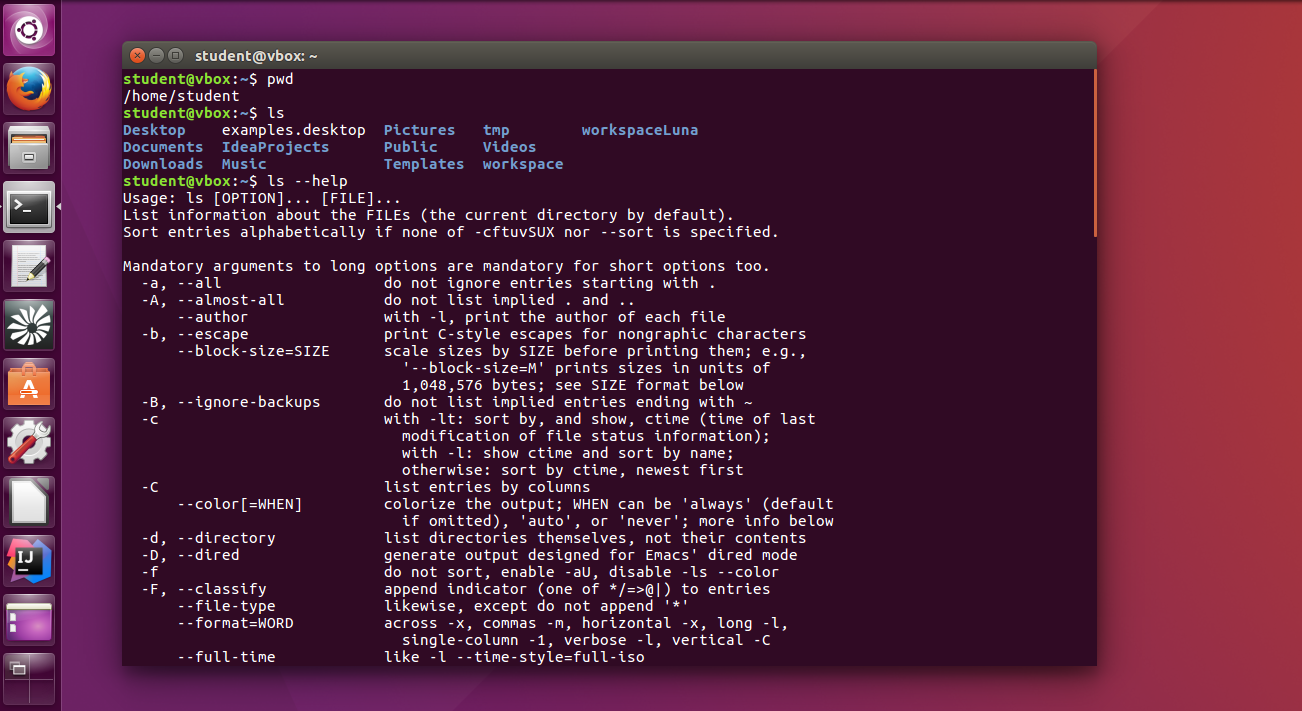
\includegraphics[width=1.0\textwidth]{../img/linux-terminal.png}
    \caption{Terminalfönster i Ubuntu öppnas med Ctrl+Alt+T.}
    \label{fig:terminal:linux}
    \end{figure}

I Ubuntu trycker du lättast \textbf{Ctrl+Alt+T} eller sök efter ''terminal'' i app-menyn.  Då öppnas ett fönster med en blinkande markör som visar att det är redo att ta emot dina textkommando. Ett exempel på kommando är \texttt{ls} som skriver ut en lista med filer i det aktuella biblioteket, så som visas i fig. \ref{fig:terminal:linux}.

Det som visas i ett terminalfönster sköts av ett \textbf{kommandoskal} \Eng{command shell}, som är redo att ta emot kommando efter en prompt som slutar med ett \texttt{\$}-tecken. När du skriver ett kommando och trycker Enter anropar kommandoskalet en kommandotolk som tolkar och utför dina kommandon. Om ett kommando inte kan tolkas, skrivs ett felmeddelande. 

Det finns många användbara kortkommando, varav de viktigaste visas i tabell \ref{fig:terminal:shortcuts}. Det är bra om du lär dig dessa kortkommandon utantill så att ditt arbete i terminalen går snabbt och smidigt.

\begin{table}[H]
\renewcommand{\arraystretch}{1.15}
\begin{tabular}{@{}r | l}
pil upp/ner & bläddra i kommandohistoriken \\
Tab & ''auto-complete'', fyll i resten baserat på vad du skrivit hittills \\
Tab Tab & två tryck på Tab listar flera alternativ, om så finnes \\
Ctrl+A & ''ahead'', flytta markören till början av raden \\
Ctrl+E & ''end'', flytta markören till slutet av raden \\
Ctrl+K & ''kill'', ta bort tecken från markören till radens slut\\
Ctrl+U & ''undo'', ta bort tecken från markören till början av raden \\
Ctrl+Y & ''yank'', sätt in det som senast togs bort\\
Ctrl+Z & ''zleep'', stoppa pågående process, skriv sedan \texttt{bg} för bakgrundskörning\\
Ctrl+L & rensa terminalfönstret\\
Ctrl+D & avsluta kommandoskalet \\
\end{tabular}
    \caption{Viktiga kortkommandon i Linux terminalfönster.}
    \label{fig:terminal:shortcuts}
\end{table}

\noindent Ctrl+C orsakar normalt ett avbrott av pågående process, men om du vill att Ctrl+C ska vara ''Copy'' som vanligt för att kopiera markerad text, kan du ställa om detta med terminalförnstrets  meny ''Edit $\rightarrow$ Keyboard Shortcuts'', eller liknande.




 
\subsubsection{PowerShell, Cmd och Linux i Microsoft Windows}
Microsoft Windows är inte Linux-baserat, men i kommandotolken \textbf{Powershell} finns alias definierade för några vanliga Linux-kommandon, inkluderat \texttt{ls}, \texttt{cd} och \texttt{pwd}. 
Du startar Powershell t.ex. genom att trycka på Windows-knappen och skriva \texttt{powershell}. 
Du kan också, medan du bläddrar bland filer, klicka på filnamnsraden överst i filbläddraren och skriva \texttt{powershell} och tryck Enter; då startas Powershell i aktuellt bibliotek. Ändra gärna typsnitt och bakgrundsfärg med hjälp av fönstrets menyer, så att det blir lättare för dig att läsa vad som skrivs.

Det finns även i Windows den ursprungliga kommandotolken \textbf{Cmd} med helt andra kommandon. Till exempel skriver man i Cmd kommandot \texttt{dir} i stället för \texttt{ls} för att lista filer. 

I Windows 10 kan du (numera, om du installerad senaste uppdateringarna av Windows) även köra Ubuntu-terminalen med hjälp av Windows Linux Subsystem (WSL). Se vidare här om hur du kan installera WSL under Windows 10: 

\url{https://ubuntu.com/wsl} 

Läs mer här: \href{https://www.omgubuntu.co.uk/2020/03/windows-10-linux-kernel-update}{www.omgubuntu.co.uk/2020/03/windows-10-linux-kernel-update}



\subsubsection{Terminal i Apple macOS/OS X}


Apple OS X och macOS är Unix-baserade operativsystem. De flesta vanliga terminalkommandon som fungerar i Linux fungerar också under Apple OS X och macOS. Du startar ett terminalfönster i Apples operativsystem genom att klicka på förstoringsglaset uppe till höger, skriva \texttt{terminal}, och trycka Enter.

\section{Vad är en path/sökväg?}\label{terminal:path}

När du skriver ett kommando i terminalen, eller kör vilket program som helst på din dator, behöver operativsystemet identifera i vilken fil programmets maskinkod ligger innan programmet kan köras. 

Lokaliseringen av filer sker med hjälp av en \textbf{sökväg} \Eng{path}, som anger en position i filsystemet. Ofta betraktas filsystemet som ett upp-och-ned-vänt träd, och kallas därför även ''filträdet''. Den ''översta'' positionen kallas ''rot'' \Eng{root} och betecknas med ett enkelt snedstreck \texttt{/}. Kataloger som ligger i kataloger utgör förgreningar i trädet. En sökväg pekar ut vägar genom trädet som behövs för att nå ''löven'', som utgörs av själva filerna.

Du kan se var ett program ligger i Linux med hjälp av kommandot \texttt{which} enligt nedan.\footnote{Skriv \texttt{ gcm ls } i Windows Powershell för motsvarighet till \texttt{ which ls } \\ Eller skriv \texttt{ New-Alias which get-command } för tillgång till kommandot \texttt{which} i Powershell. \\ \href{http://stackoverflow.com/questions/63805/equivalent-of-nix-which-command-in-powershell}{stackoverflow.com/questions/63805/equivalent-of-nix-which-command-in-powershell}} Listan med bibliotek i sökvägen avskiljs med snedstreck.
\begin{REPLnonum}
$ which java
/usr/lib/jvm/oracle_jdk8/bin/java
$ which ls
/bin/ls
\end{REPLnonum}

En sökväg kan vara \textbf{absolut} eller \textbf{relativ}. En absolut sökväg utgår från roten och visar hela vägen från rot till destination, t.ex. \texttt{/usr/bin/firefox}, medan en relativ sökväg utgår från aktuellt bibliotek (där du ''står'') och börjar \textit{inte} med ett snedstreck.

Alla operativsystem håller reda på en mängd olika sökvägar för att kunna hitta speciella filer i filträdet. Dessa sökvägar lagras i s.k. \textbf{miljövariabler} \Eng{environment variables}. Det finns en \textit{speciell} miljövariabel som heter kort och gott \textbf{PATH}, i vilken alla sökvägar till de program finns, som ska vara tillgängliga för din användaridentitet direkt för exekvering genom sina filnamn, \textit{utan} att man behöver ange absoluta sökvägar. 

Du kan i Linux se vad som ligger i din PATH med kommandot \code{ echo $PATH } medan man i Windows Powershell skriver \code{$env.Path} där det bara är första bokstaven som ska vara en versal. I Linux separeras biblioteken i sökvägen med kolon, medan Windows använder semikolon.

Ibland kan du behöva uppdatera din PATH för att program som du installerat och ska bli allmänt tillgängliga. Detta görs på lite olika sätt i olika operativsystem, för Linux se t.ex. här:
\href{http://stackoverflow.com/questions/14637979/how-to-permanently-set-path-on-linux}{stackoverflow.com/questions/14637979/how-to-permanently-set-path-on-linux}

När man anger sökvägar finns några tecken med speciell betydelse:

\begin{tabular}{r  p{0.8\textwidth}}
\code|~| & ''tilde'', din hemkatalog \\
\code|/| & ''slash'', snedstreck anger filträdets rot om det finns i början av sökvägen, men utgör biblioteksavskiljare inuti sökvägen \\
\code|.| & en punkt anger aktuellt bibliotek, där du ''står'' \\
\code|..| & två punkter anger ett steg ''upp'' i filträdet \\
\code|"| & omgärda en sökväg med citationstecken, först och sist, om den innehåller annat än engelska bokstäver, t.ex. blanktecken\\
\code|\ | & \textit{backslash+blanktecken} används för att beteckna mellanslag i sökvägar som \textit{inte} omgärdas av citationstecken\\
\end{tabular}

\section{Några viktiga terminalkommando}

I tabell \ref{fig:terminal:commands} finns en lista med några viktiga terminalkommando som är bra att lära sig utantill.

En introduktion till LTH:s datorer med exempel på hur du använder vanliga Linux-kommandon finns i denna skrift \url{http://www.ddg.lth.se/perf/unix/} som används i introduktionsveckan för nybörjare på datateknikprogrammet vid LTH.

På sajten \url{http://ss64.com/} finns en mer omfattande lista med användbara terminalkommando och tillhörande förklaringarför för Linux (Bash), Windows (Powershell, Cmd) och Apple OS X (Bash).  

\begin{table}[H]
\renewcommand{\arraystretch}{1.25}
   
\begin{tabular}{@{}r | l}
\texttt{ls} & lista filer i aktuellt bibliotek (alltså där du ''står'')\\
\texttt{ls} \textit{p}  & lista filer i biblioteket  \textit{p} \\
\texttt{ls -A} & lista alla filer i aktuellt bibliotek, även gömda \\
\texttt{man ls} & manual för kommandot \texttt{ls}; testa även \texttt{man} för andra kommandon! \\
\texttt{cd} \textit{p} & ''change directory'', ändra aktuellt bibliotek till \textit{p}\\
\texttt{pwd} & ''print working directory'', skriv ut sökväg för aktuellt bibliotek \\
\texttt{cp} \textit{p1 p2} & ''copy'', kopiera filen med path \textit{p1} till en ny fil kallad \textit{p2} \\
\texttt{mv} \textit{p1 p2} & ''move'', byt namn på filen \textit{p1} till \textit{p2}  \\
\texttt{rm} \textit{p} & ''remove'', ta bort filen \textit{p}\\
\texttt{rm -r} \textit{p} & ''remove recursive'', ta bort biblioteket \textit{p} med allt innehåll; var försiktig!\\
\texttt{mkdir} \textit{p} & ''make dir'', skapa ett nytt bibliotek \textit{p}\\
\texttt{cat} \textit{p1 p2}& ''concatenate'', skriv ut hela innehållet i en eller flera filer \textit{p1 p2 etc.}\\
\texttt{less} \textit{p}& skriv ut innehållet i filen \textit{p}, en skärm i taget\\
\texttt{wget} \textit{url}&ladda ner \textit{url}, t.ex. \texttt{ wget http://cs.lth.se/pgk/ws -o ws.zip}\\
\texttt{unzip} \textit{p}& packa upp \textit{p}, t.ex. \texttt{ unzip ws.zip}\\
\end{tabular}

    \caption{Några viktiga terminalkommando i Linux. Med \textit{p}, \textit{p1}, \textit{p2}, etc.  avses en absolut eller relativ sökväg \Eng{path}, se avsnitt \ref{terminal:path}.}
    \label{fig:terminal:commands}

\end{table}


%!TEX encoding = UTF-8 Unicode
%!TEX root = ../compendium.tex

\chapter{Kompilera och exekvera}\label{appendix:compile}

\section{Vad är en kompilator?}

En \textbf{kompilator} \Eng{compiler} är ett program som läser programtext och översätter den till exekverbar maskinkod, så som visas i figur \ref{fig:appendix:compiler}. Programtexten som kompileras kallas källkod och utgörs av text som följer reglerna för ett programmeringsspråk, till exempel Scala eller Java. 

\begin{figure}[H]
\centering
\begin{tikzpicture}[node distance=1.8cm, scale=1.5]
\node (input) [startstop] {\bf\sffamily Källkod};
\node(inptext) [right of=input, text width=2cm, xshift=1.5cm]{För\\människor};
\node (compile) [process, below of=input] {\bf\sffamily Kompilator};
%\node(explain) [right of=compile, text width=5cm, xshift=3.0cm]{Översätter från källkod till maskinkod};
\node (output) [startstop, below of=compile] {\bf\sffamily Maskinkod};
\node(outtext) [right of=output, text width=2cm, xshift=1.5cm]{För\\maskiner};
\draw [arrow] (input) -- (compile);
\draw [arrow] (compile) -- (output);
\end{tikzpicture}
    \caption{En kompilator översätter från källkod till maskinkod.}
    \label{fig:appendix:compiler}
\end{figure}




Vissa kompilatorer genererar kod som kan köras av en processor direkt, medan andra kompilatorer genererar ett mellanformat som tolkas under exekveringen. Det senare är fallet med Java och Scala, vilket möjliggör att programmet kan kompileras en gång för alla plattformar och sedan kan programmet köras på all de processorer till vilka en s.k. virtuell maskin för Java finns \Eng{Java Virtual Machine, JVM}. Den kod som genereras av en kompilator som kodgenererar för JVM kallas \textbf{bytekod}.

Om kompileringen inte lyckas skriver kompilatorn ut ett felmeddelande och ingen maskinkod genereras. Det är inte lätt att bygga en kompilator som ger bra felmeddelanden i alla lägen, men felmeddelandet ger oftast goda ledtrådar till felorsaken efter att man lärt sig tolka det programmeringsspråksspecifika vokabulär som kompilatorn använder.

Även om programmet kompilerar utan felmeddelande och genererar exekverbar maskinkod, är det vanligt att programmet ändå inte fungerar som det är tänkt. Ibland är det mucket svårt att lista ut vad problemet beror på och man kan behöver göra omfattande undersökningar av vad som händer under körningen, genom att t.ex. skriva ut olika variablers värden eller på annat sätt ändra koden och se vad som händer. Denna process kallas felsökning eller avlusning \Eng{debugging}, och är en väsentlig del av all systemutveckling. 

En uttömmande testning av ett större program, som kör programmets \textit{alla} möjliga exekveringsvägar, är i praktiken omöjlig att genomföra inom rimlig tid, då antalet kombinationsmöjligheter växer mycket snabbt med storleken på programmet. 
Därför är kompilatorn ett mycket viktigt hjälpmedel. Med hjälp av den analys och de kontroller som görs av kompilatorn kan många buggar, som annars vore mycket svåra att hitta, undvikas och åtgärdas i kompileringsfasen, redan \textit{innan} man exekverar programmet. 


\section{Java JDK}

Scala, Java och flera andra språk använder Java-plattformen som exekveringsmiljö. Om man inte bara vill köra program som andra har utvecklat, utan även utveckla egna program som fungerar i denna miljö, behöver man installera Java Develpment Kit (JDK). Detta utvecklingspaket innehåller flera delar, bland annat:

\begin{itemize}

\item Kompilatorn \texttt{javac} kompilerar Java-program till bytekod som lagras i klassfiler med filnamnsändelsen \texttt{.class}.

\item Exekveringsmiljön Java Runtime Enviroment (JRE) med kommandot \texttt{java} som drar igång den virtuella javamaskinen (Java Virtual Machine) som kan ladda och exekvera bytekod lagrade i klassfiler.

\item Programmet \texttt{jar} som packar ihop många sammanhörande klassfiler till en enda jar-fil som lätt kan distribueras via nätet och sedan köras med \texttt{java}-kommandot på alla maskiner med JRE. 

\item Programmet \texttt{javap} som läser klassfiler och skriver ut vad de innehåller i ett format som kan läsas av människor (ett sådant program kallas disassembler).

\item I JDK ingår också en mycket stor mängd färdiga programbibliotek med stöd för nätverkskommunikation, filhantering, grafik, kryptering och en massa annat som behövs när man bygger moderna system. 

\end{itemize}  

\noindent Du kan läsa mer om Java och dess historik här: \\
\href{https://en.wikipedia.org/wiki/Java_(programming_language)}{https://en.wikipedia.org/wiki/Java\_(programming\_language)}

\subsection{Kontrollera om du har JDK installerat}\label{appendix:compile:check-jdk}

Öppna ett terminalfönster (se appendix \ref{appendix:terminal}) och skriv (observera det avslutande c:et i \texttt{javac}):
\begin{REPLnonum}
javac -version
\end{REPLnonum}
Då ska ungefär följande skrivas ut (där siffran 101 kan vara något annat):
\begin{REPLnonum}
javac 1.8.0_101
\end{REPLnonum}
Om utskriften säger att javac saknas, installera JDK8 enl. nedan.

Du kanske redan har enbart Java Runtime Environment (JRE) installerad, men inte JDK. Då saknar du javakompilatorn javac m.m. och behöver installera JDK, se nedan. Du kan kolla om du har JRE genom att skriva \texttt{java -version} (alltså utan c efter java). Eller så har du redan JDK installerad men inte rätt bibliotek i din PATH; se vidare nedan ang. uppdatering av PATH.



\subsection{Installera JDK}\label{appendix:compile:install-jdk}

Det finns flera JDK-distributioner att välja mellan, varav Oracle JDK och Azul Zulu OpenJDK är två exempel. Oracle JDK har störst spridning och är förinstallerad på LTH:s datorer. För att installera JDK på din egen dator behöver du gå igen flera steg, som behöver anpassas efter det operativsystem du kör, enligt nedan. 
På kurshemsidan under ''Verktyg'' finns kompletterande instruktioner:  \url{http://cs.lth.se/pgk/verktyg} 


Din användaridentitet behöver ha administratörsrättigheter för att du ska kunna genomföra installationen.



\subsubsection{Linux} 
För Ubuntu: läs först noga igenom och följ sedan dessa instruktioner till punkt och pricka: \\ \href{http://www.webupd8.org/2012/09/install-oracle-java-8-in-ubuntu-via-ppa.html}{www.webupd8.org/2012/09/install-oracle-java-8-in-ubuntu-via-ppa.html}

För andra Linux-distributioner, kör detta i terminalen (funkar även i Ubuntu men du får med detta kommando inte Oracles aningen snabbare JVM): \\ \texttt{sudo apt-get install openjdk-8-jdk}

\subsubsection{Windows/macOS}

\begin{enumerate}
\item Installera senaste JDK från Oracle. Om du inte har installerat JDK förr på din dator så be gärna någon kurskamrat med erfarenhet av detta att assistera dig medan du följer stegen nedan. 

\begin{enumerate}
\item Surfa till Oracles hemsida för Java SE här: \\ \url{http://www.oracle.com/technetwork/java/javase/downloads/}

\item Klicka på rubriken ''Java SE 8u101 / 8u102'' och på nästa sida klicka på knappen ''Accept License Agreement'' i listan under rubriken ''Java SE Development Kit 8u101''. (Siffrorna 101 eller 102 kan vara annorlunda om senare versioner tillkommit.)

\item Välj rätt version av operativsystem (Windows x64 eller Mac OS X). Det är viktigt att du väljer x64, d.v.s 64-bitarsvarianten som gäller för alla moderna datorer.

\item Klicka på länken och en stor fil kommer laddas ner till din dator.

\item Installera när filen laddats färdigt. 

\end{enumerate}

\item Uppdatera PATH, så att du får tillgång till alla kommando i terminalen:
\begin{itemize}
\item För Windows görs detta enklast genom att ladda ner och sedan köra denna fil genom att dubbelklicka på den: \\ \url{https://github.com/lunduniversity/introprog/raw/master/tools/windows-jdk-set-path.bat}
\item För macOS, läs här: \\ \href{https://docs.oracle.com/javase/8/docs/technotes/guides/install/mac_jdk.html}{docs.oracle.com/javase/8/docs/technotes/guides/install/mac\_jdk.html}

\item Om något krånglar, be om hjälp. Om du vill veta mer om PATH-uppdatering för java, läs här:\\ \url{https://java.com/sv/download/help/path.xml} \\
Om du kör engelska menyer byt \texttt{sv} mot \texttt{en} i adressen ovan.  Du kan ta reda på vilken katalog som ska läggas in sist i din PATH efter ett semikolon genom att bläddra bland dina systemfiler och undersöka var JDK har installerats; i Windows antagligen något liknande detta (kolla exakt vilket versionsnummer du har): \code|C:\Program Files\Java\jdk1.8.0_101\bin|
\end{itemize}

\item Starta om datorn. Det är först efter att en ny användarinloggning initierats, som PATH-tilldelningen får effekt.

\item Kontrollera att \texttt{javac} fungerar enligt avsnitt \ref{appendix:compile:check-jdk}.
\end{enumerate}


\section{Scala}

Scala använder JDK som exekveringsmiljö, men erbjuder ytterligare verktyg specifika för Scala. I utvecklingspaketet för Scala ingår bl.a. kompilatorn \texttt{scalac} och även ett interaktivt kommandoskal kallat Scala REPL där du kan testa din Scala-kod rad för rad och se vad som händer direkt. 

De flesta av kursens övningar görs i Scala REPL, medan laborationerna kräver kompilering av lite större program.

Du hittar mer om Scalas historik och annan bakgrundsinformation här: \mbox{%
 \href{https://en.wikipedia.org/wiki/Scala_(programming_language)}{en.wikipedia.org/wiki/Scala\_(programming\_language)}
}

\subsection{Installera Scala}

Scala finns förinstallerat på LTH:s datorer. Du installerar Scala-kompilatorn och den interaktiva kodexperimentmiljön Scala REPL på din egen dator enligt nedan. 

\begin{enumerate}
\item Kontrollera att du har JDK installerad enligt avsnitt \ref{appendix:compile:check-jdk} och installera vid behov enligt avsnitt \ref{appendix:compile:install-jdk}.
\item Surfa till denna hemsida för nedladdning av Scala 2.11.8: \\ \url{http://scala-lang.org/download/2.11.8.html}
\item Klicka på ''Download'' av den variant som är relevant för ditt operativsystem och spara filen:

\begin{enumerate}
\item \textbf{Linux Ubuntu}: Filen heter \texttt{scala-2.11.8.deb} och installeras genom att dubbelklicka på filen eller via terminalkommandot:\\ \code{sudo apt install ~/Downloads/scala-2.11.8.deb} \\ anpassa sökvägen ovan efter var du sparade filen 
\item \textbf{Windows}: Filen heter \texttt{scala-2.11.8.msi} och installationen startas med ett dubbelklick. Följ instruktionerna. Installationsprogrammet uppdaterar även din PATH åt dig och allt bör fungera efter omstart.
\item \textbf{macOS}: Filen heter \texttt{scala-2.11.8.tgz} och kan packas upp på lämpligt ställe med terminalkommandot \texttt{tar -xvzf scala-2.11.8.tgz} och sedan är det underkatalogen \texttt{bin} som ska inkluderas i din PATH. \TODO klura ut säkraste rådet för path-uppdatering på mac.
\end{enumerate}
Kontrollera att terminalkommandot \texttt{scala} fungerar för att starta Scala REPL:
\end{enumerate}
\begin{REPLnonum}
$ scala
Welcome to Scala 2.11.8 (Java HotSpot(TM) 64-Bit Server VM, Java 1.8.0_101).
Type in expressions for evaluation. Or try :help.

scala> println("hej")
hej

scala>
\end{REPLnonum}
 

\subsection{Scala Read-Evaluate-Print-Loop (REPL)}\label{appendix:compile:REPL}

För många språk, t.ex. Scala och Python, finns det en interaktiv tolk som gör det möjligt att exekvera enstaka programrader och direkt se effekten. En sådan tolk kallas Read-Evaluate-Print-Loop eftersom den läser en rad i taget och översätter till maskinkod som körs direkt.    

\TODO Kortkommandon: Ctrl+K etc.

\TODO :paste








%!TEX encoding = UTF-8 Unicode
%!TEX root = ../compendium1.tex

\chapter{Fixa buggar}\label{appendix:debug}

\begin{figure}[H]
\centering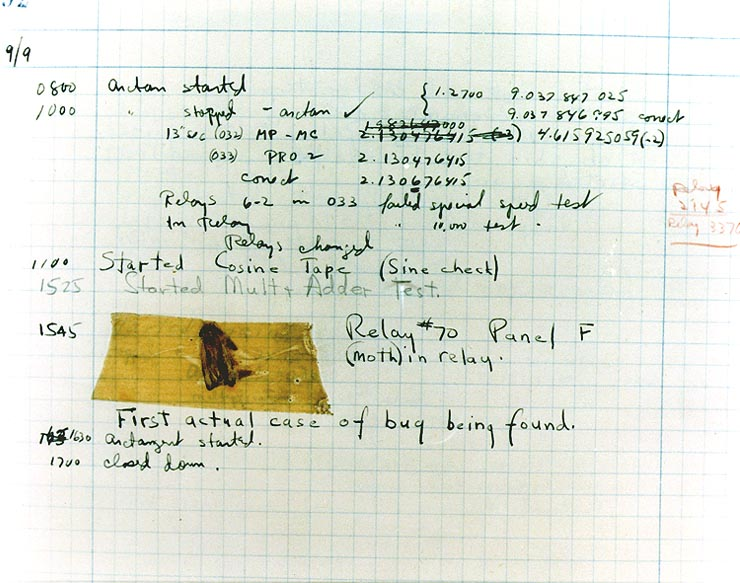
\includegraphics[width=0.85\textwidth]{../img/bug}

\caption{Den första dokumenterade buggen hittades 9 september 1947 i en Mark II Aiken Relay Calculator av Grace Hopper.\protect\footnotemark}

\end{figure}\footnotetext{\href{https://commons.wikimedia.org/w/index.php?curid=165211}{commons.wikimedia.org/w/index.php?curid=165211} Courtesy of the Naval Surface Warfare Center, Dahlgren, VA., 1988. - U.S. Naval Historical Center Online Library Photograph NH 96566-KN, Public Domain.   }


\section{Vad är en bugg?}

En bugg, även kallad lus \Eng{bug}, är en felaktighet som kan göra så att ett program inte beter sig som det är tänkt, och kan innebära oönskad utdata, att programmet kraschar, eller till och med ond bråd död.\footnote{\href{https://www.theguardian.com/technology/2016/jul/01/tesla-driver-killed-autopilot-self-driving-car-harry-potter}{www.theguardian.com/technology/2016/jul/01/tesla-driver-killed-autopilot-self-driving-car-harry-potter}}

Ursprunget till ordets användning i programmeringssammanhang är något oklar, men kan härledas till engelskans \emph{bug} som betyder insekt eller småkryp. 
Man brukar berätta att vid en felsökning av ett program som körde i en tidig dator byggd med  elektromekaniska reläer, uppdagades en död nattfjäril ihjälklämd mellan drivankaret och spolen i ett relä, som orsakade att programmet inte kunde exekveras korrekt. 



\subsection{Olika sorters fel}

När man ska lära sig mer om fel i programvarubaserade system, och hur de kan åtgärdas, är det viktigt att noga skilja på \textbf{misstag} \Eng{mistake}, \textbf{felorsak} \Eng{fault} och \textbf{felyttring} \Eng{failure}. 
Med ''misstag'' menar vi här ett fel som begås av människor (utvecklare, systemadministratörer, operatörer, användare, etc.) medan de skapar och använder ett programvarusystem. 

Det kan bli fel i olika delar av processen: 
\begin{itemize}
\item \textbf{Kravfel} uppstår medan man tänker ut vad systemet ska göra och då misstar sig angående  användarnas behov och önskemål.
\item \textbf{Designfel} uppkommer när man utformar systemets struktur på ett dåligt sätt.
\item \textbf{Implementeringsfel} begås när man programmerar och skriver felaktiga kodrader. 
\item \textbf{Testfel} förekommer vid provkörning av systemet då testkoden är felaktig och därför ger falskt alarm om ''fel'', trots att beteendet egentligen är korrekt.  
\item \textbf{Operatörsfel} sker när systemet lämnas över till de, som ska installera och köra systemet i skarp produktion, och där systemdriften \Eng{operations, ''ops''} sköts på ett sätt som får problematiska konsekvenser.
\item \textbf{Användarfel} händer då användarna ger felaktig indata, eventuellt i strid med riktlinjerna för hur systemet ska användas, som systemet inte klarar att hantera korrekt, varpå mer eller mindre allvarliga felbeteenden hos systemet följer.
\end{itemize} 
I olika delar av utvecklingsprocessen kan alltså misstag begås som, antingen omedelbart, eller någon gång i framtiden, kan orsaka fel. Men det är inte säkert att ett fel någonsin kommer att märkas. Kanske kommer de felaktiga kodraderna, som \emph{skulle} kunna orsaka ett fel, aldrig att exekveras. Eller så kommer ingen användare att någonsin vilja använda systemet så som stipuleras av (onödiga) krav. Det är alltså först när fel \emph{yttrar} sig vid exekvering som misstag märks.

Fel kan också kategoriseras utifrån \emph{hur} de upptäcks i utvecklingsprocessen. Man brukar skilja på fel upptäckta vid granskning, kompileringsfel och exekveringsfel, som diskuteras nedan:
\begin{itemize}
\item Fel upptäckta vid \textbf{granskning}. Ett effektivt sätt att upptäcka fel är att människor noga läser igenom sin egen, och andras kod och försöker leta efter möjliga problem och brister. Man blir ofta ''hemmablind'' när det gäller ens egen kod. Därför kan någon annans, oberoende granskning med ''nya, friska'' ögon vara mycket fruktbar.  I samband med kodgranskning kan man med fördel försöka bedöma  huruvida koden är lätt att läsa, lätt att ändra i eller om koden har andra viktiga kvaliteter som har betydelse för den framtida utvecklingen av koden. Ofta hittar man vid granskning även enkla programmeringsmisstag, så som felaktiga villkor och loop-räknare som inte räknas upp på rätt sätt etc.
  
\item \textbf{Kompileringsfel} uppkommer under kompilering och upptäcks tack vare kontroller som sker av  kompilatorn. 

Vid kompileringsfel får man också ofta av kompilatorn reda på \emph{var} i koden det är fel och \emph{varför} det är fel, så att sökandet efter felorsaken och åtgärdandet av misstaget underlättas. Men ibland är felmeddelandet från kompilatorn missvisande och pekar på helt fel ställe i koden, så det gäller att inte alltid lita blint på det kompilatorn skriver. Dessutom är felmeddelanden från kompilatorn ofta uttryckta i termer av språkets syntaktiska och semantiska regler och det tar tid att lära sig tolka kompilatorers felmeddelanden. Att skapa kompilatorer som ger bra felmeddelande är ett svårt problem som studeras inom den datavetenskapliga disciplinen \textit{kompilatorteknik}, vilken du kan lära mer om i kurser på avancerad nivå.

Olika programmeringsspråk erbjuder olika stora möjligheter att göra kontroller vid kompileringstid. En kompilator för ett språk med ett avancerat typsystem, som till exempel Scala, ger förhållandevis stora möjligheter att identifiera fel redan under kompileringen, medan man med ett språk med ett svagare typsystem, till exempel Javascript, får förlita sig på prestandahämmande kontroller som kompilatorn genererar i maskinkoden eller som du själv väljer att lägga in i källkoden för säkerhets skull. 
  
\item \textbf{Exekveringsfel}, även kallat körtidsfel \Eng{runtime error}, sker medan programmet körs. Det kan krävas viss, specifik indata under specifika exekveringsomständigheter (en viss processor, en viss minnesstorlek, en viss nätverkskapacitet etc.) för att ett exekveringsfel ska yttra sig. När ett exekveringsfel väl yttrar sig, kan olika saker hända:

\begin{itemize}

\item \textbf{Exekveringen ger oönskat resultat.} Det är inte säkert att ett exekveringsfel avbryter exekveringen; det är vanligt att felet ''bara'' resulterar i inkorrekt utdata eller på annat sätt ger dålig kvalitet. För att upptäcka detta innan systemet sätts i drift, är det allmän praxis att man skriver noga uttänkta \textbf{testfall} och analyserar \textbf{testresultat} från exekveringen av  testfallen i detalj genom att undersöka utdata i jämförelse med önskat resultat eller med vad som anses vara en tillräckligt hög kvalitetsnivå.

\item \textbf{Exekveringen hänger sig} \Eng{hang}. Ibland yttrar sig fel genom att inget alls ser ut att hända under exekveringen, vilket kan beror på t.ex.:  
\begin{itemize}[nolistsep]
\item en \textbf{oändlig loop}, som aldrig blir färdig, 
\item att det går \textbf{väldigt långsamt} eftersom bearbetningen av indata tar orimligt lång tid,
\item att programmet \textbf{väntar på indata} som aldrig kommer,
\item att olika jämlöpande delar av programmet väntar på varandra så att ett \textbf{dödläge} \Eng{deadlock} uppstår. 
\end{itemize}

När exekveringen hänger sig och man inte orkar vänta längre på att något ska hända, är det bara att brutalt avbryta exekveringen genom något lämpligt kommando som erbjuds i din körmiljö.\footnote{\texttt{kill -9} $<$pid$>$, Ctrl+C, Ctrl+Shift+C, Ctrl+Z eller något annat beroende på körmiljö.} I värsta fall får man stänga av strömmen.

\item \textbf{Exekveringen kraschar} \Eng{crash}. Ibland blir det ett plötsligt tvärstopp och exekveringen avbryts med ett körtidsfelmeddelande. Detta kan bero på t.ex.:
\begin{itemize}[nolistsep]
\item att \textbf{minnet är slut}, antingen är det parameterminnet för funktionsanrop \Eng{stack memory} som tagit slut eller så är minnet för allokering av objekt som skapas under programmets gång \Eng{heap memory} fullt,
 
\item misstaget att försöka referera en \textbf{null-referens} som inte refererar till något objekt, utan har värdet \code{null}, vilket resulterar i  \textit{null pointer exceeption},

\item att ett s.k. \textbf{undantag} har ''kastats'' \Eng{throw exception} genom att den som skrivit programmet medvetet kodat så att ett oönskat feltillstånd \emph{ska} orsaka en krasch, om inte undantaget ''fångas'' \Eng{catch} och hanteras av omgivande kod. 
\end{itemize}

När systemet kraschar får man en lista med den aktuella kedjan av funktionsanrop i en \textbf{stackspårning} \Eng{stack trace}. Man kan också begära en utskrift av hela innehållet i minnet vid kraschen \Eng{memory dump}, men en sådan kan vara svår att tolka.

\end{itemize}

\end{itemize}

När systemet ger oönskade resultat, hänger sig eller kraschar, får man försöka återskapa exekveringsfelet i en omkörning och, med hjälp av instrumentering eller en debugger, försöka lista ut vad som händer precis \emph{innan} exekveringsfelet uppstår, se  avsnitt \ref{section:debugging}.

I kursen \textit{Programvarutestning} \Eng{Software Testing} lär du dig mer om systematiska metoder för att testa system så att fel kan förebyggas, identifieras och åtgärdas.

\subsubsection{Bugg eller feature?} 

När ett (eventuellt) fel upptäcks, kan det vara på sin plats att först ställa sig några grundläggande  frågor:

\begin{itemize}
\item Är detta verkligen ett ''fel'' eller är det egentligen ett avsett beteende? Det är inte alltid självklart om det är en bugg eller en medvetet skapad systemegenskap/funktion \Eng{feature}.

\item Är det kanske testfallet som har felaktig testkod, medan koden som testas egentligen fungerar alldeles utmärkt? Sådan problem kan vara speciellt svåra att lösa, då man ofta letar på fel ställe efter orsaken.

\item Om buggen rör någon kvalitetsegenskap hos systemet kan man fråga sig: Var går egentligen gränsen för ''fel''? Är detta bra nog givet vad det kostar att förbättra kvaliteten? Kvalitetskrav berör egenskaper hos ett program som kan uttryckas på en glidande skala, där något kan vara mer eller mindre \emph{bra} eller \emph{dåligt} ur olika synvinklar. Sådana krav leder ofta till viktiga men svåra avvägningsbeslut under design och implementation. Dessutom kan testresultat bli svårbedömda och det kan finnas olika åsikter om huruvida ett eventuellt fel är en bugg eller inte.

Här är några exempel på kvalitetskrav:
\begin{itemize}
\item \textbf{Prestandakrav} \Eng{performance requirements} avser hur snabbt och effektivt programmet ska arbeta under olika omständigheter.
 
\item \textbf{Kapacitetskrav} \Eng{capacity requirements} avser hur mycket data systemet ska klara av under olika omständigheter.

\item \textbf{Användbarhetskrav}\footnote{\href{https://sv.wikipedia.org/wiki/Anv\%C3\%A4ndbarhet}{sv.wikipedia.org/wiki/Användbarhet}} \Eng{usability requirements} avser krav på hur lättanvänt systemet ska vara för en given användarkategori. 
\end{itemize} 

\end{itemize}

I kursen \textit{Kravhantering} \Eng{Sofware Requirements Engineering} lär du dig mer om att identifiera, specificera och följa upp kvalitetskrav.

\subsubsection{Felärendehanteringsverktyg} 

Det är allmän praxis i industriell systemutveckling att använda sig av ett felärendehanteringsverktyg \Eng{issue tracker} så att samarbetande utvecklare får stöd i att hålla reda på alla uppkomna fel och problem \Eng{issue}. Många av de populära kodlagringsplatserna som finns på nätet, så som GitLab, GitHub och BitBucket (se avsnitt \ref{section:code-hosting}), erbjuder felärendehanteringsfunktioner. Dessa kan till exempel vara:
\begin{itemize}
\item hantering och sammanställning av alla olika ärendetillstånd, så att man kan se vilka issues som är i tillstånden \textit{Open} eller \textit{Closed},
\item tillording av ärende till specifika personer som ska åtgärda problemet,
\item gradering av ärende i olika allvarlighetsgrader,
\item meddelandegenerering till inblandade personer när ett ärende kommenteras eller ändrar tillstånd.
\end{itemize}


\section{Att förebygga fel}

Även om det nästan är oundvikligt att inte låta buggar slinka in i koden allteftersom den blir mer och mer komplex, är det ändå viktigt att lägga stor möda vid att försöka undvika att så sker. Det är ofta mycket bättre investerad tid att jobba med buggförebyggande åtgärder medan du skapar koden, än att jaga buggar som skulle kunna ha undvikts med allmän noggrannhet och stramare disciplin i kodningen. Nedan sammanfattas några åtgärder som kan hjälpa till att minska mängden fel.

\begin{itemize}
\item \textbf{Skapa begriplig kod}. Grunden för att undvika buggar är anstränga sig att skriva begriplig kod som är lätt att läsa. Detta är en ständig kamp; kodens komplexitet växer för varje tillägg och med jämna mellanrum behövs omstruktureringar \Eng{refactoring} för att bibehålla en god struktur som underlättar begripligheten och gör utvidgningar lättare. 
%En integrerad utvecklingsmijlö erbjuder stöd för att omstrukturera kod  med bibehållen korrekthet. 

\item \textbf{Tänk ut bra namn}. En viktig pusselbit för att skapa begriplig kod är att tänka ut bra namn. Detta kan vara förvånansvärt svårt och kan kräva mycket diskussioner och tankemöda. 
%I själva namnet ligger ofta en stor del av möjligheten för en abstraktion du skapat att nå ut till dina medutvecklare med rätt associationer, som genom sitt namn antingen kan skapa härligt läsbar programtext, eller oerhört svårigenomtränglig gröt där namnen snarast upplevs som desinformation. 
Om du inser att ett namn är illa valt är det förmodligen värt jobbet att omstrukturera koden och införa ett bättre namn, speciellt om andra ännu inte vant sig alltför mycket vid begreppet. 
%Ibland när ett namn ''kliar'' beror det på att själva abstraktionen är feltänkt och behöver tänkas om. 
%En integrerad utvecklingsmiljö erbjuder stöd för att byta namn på precis rätt ställe, med hänsyn till synlighet och blockstruktur. 

\item \textbf{Kontrollera parametrar och variabler}. Ofta vet känner man till vilka villkor som måste gälla för olika variablers värden. Till exempel vet man ofta att en viss funktionsparameter av heltalstyp inte får vara negativ. Då kan man säkerställa detta genom att lägga in kontroller av att villkoret är uppfyllt. Vid villkor som gäller parametrar, brukar man i Scala anropa \code{require}, till exempel: \code{require(x >= 0, "x must be positive")}. Det finns också en metod \code{assert} som fungerar på samma vis\footnote{\href{http://stackoverflow.com/questions/26140757/what-to-choose-between-require-and-assert-in-scala}{stackoverflow.com/questions/26140757/what-to-choose-between-require-and-assert-in-scala}}; medan \code{require} används för att kontrollerar parametrar, brukar \code{assert} användas för att kontrollera generella villkor som ska gälla, till exempel \code{assert(x + y > n, "overflow")}.  Fördelen med att lägga in kontroller av villkor är att villkorsbrott upptäcks direkt och felsökningen blir lättare. 

\item \textbf{Kontrollera typer}. Med \textit{typannoteringar} får du hjälp av kompilatorn att kontrollera dina hypoteser om vilka typer olika värden har. I Scala kan du nästan var du vill i ett uttryck lägga till ett kolon och en typ för att begära att kompilatorn kontrollerar typen. Till exempel kan du skriva \code{(xs + f(42)) : Set[Int]} för att säkerställa att uttrycket \code{xs + f(42)} verkligen ger en mängd med heltal. Även om du sällan i Scala behöver ange typer explicit, tack vare kompilatorns typinferens, bidrar det till läsbarheten och skapar säkrare kod om du på lämpliga ställen ändå anger de typer som du förväntar dig, speciellt vid i komplicerade uttryck eller långa kedjor av metodanrop, och när metoders returtyper inte är uppenbara. Dessutom kan kompilatorn ibland undvika att gå vilse i speciellt svåra typhärledningar, om du hjälper den på traven med explicita typannoteringar.

\item \textbf{Hantera saknade värden}. Det är mycket vanligt att man måste hantera situationer där ett värde saknas, inte kan beräknas, eller inte finns tillgängligt av andra orsaker. Man kan hålla reda på att ett värde saknas genom att representera detta med speciella värden, t.ex. \code{-1} eller \code{null}. Men den strategin leder mycket lätt till buggar, då man lätt glömmer att på andra ställen i koden kontrollera dessa speciella värden. Med sådana speciella värden får man heller ingen hjälp av kompilatorn att upptäcka att man missat att ta hand om dem. Om man istället hanterar eventuellt saknade värden med \code{Option} (se kapitel \ref{chapter:W08}), så får man hjälp vid kompileringstid och slipper exekveringsfel och besvärlig felsökning. Det blir dessutom väldigt tydligt för alla som läser din kod, inklusive du själv, att ett värde kan saknas.
 
\item \textbf{Hantera undantag}. När undantag uppstår, t.ex. att en fil inte kan läsas eller det blir division med noll, avbryts exekveringen och programmets användare kan inte använda programmet längre, vilket i värsta fall kan få ödesdigra konsekvenser. Därför vill man hantera undantagssituationer på ett sådant sätt att programmet blir robust och inte kraschar. Detta kan man med fördel göra genom att kapsla in undantaget i ett värde av typen \code{Try}, se kapitel \ref{chapter:W08}. I likhet med \code{Option} för saknade värden, blir det tydligt i koden att ett värde av typen \code{Try} kan innebära ett lyckat resultat (\code{Success}), eller så fallerar beräkningen (\code{Failure}) med en inkapslad, förhindrad krasch. 

\item \textbf{Granska kod}. Det är allmän praxis i industriell programvaruutveckling att göra kodgranskningar, vid vilka en grupp människor noga studerar någon annans kod och ger kommentarer och identifierar potentiella problem. Ofta har man en checklista att utgå ifrån medan man läser koden, som innehåller punkter man vill kontrollera speciellt, t.ex. begriplighet, namngivning, kontroller av parametrar, hantering av saknade värden och undantag, etc. Många organisationer har en överenskommen kodningsstandard med riktlinjer för kodens utseende och stil som alla ska följa om inte speciella skäl finns. Att sådana stilriktlinjer följs kan kontrolleras genom granskningar. Det finns också verktygsstöd för att göra sådana kontroller. Ett exempel på kodningsriktlinjer för Scala finns på den officiella dokumentationssajten\footnote{\url{http://docs.scala-lang.org/style/scaladoc.html}}. 

\item \textbf{Testa kod}. Det är allmän praxis i industriell programvaruutveckling att genomföra tester på flera olika nivåer. Man kombinerar ofta \textbf{enhetstest} \Eng{unit test} av enskilda delar av koden, med \textbf{funktionstest} \Eng{feature test} för att se så att indata i en tänkt användningssituation ger önskat resultat, och \textbf{systemtest} \Eng{system test} för att se att alla delar fungerar tillsammans under realistiska omständigheter. 

\item \textbf{Lär av användarnas upplevelser}. När koden sätts i produktion finns möjlighet att lära sig genom återkoppling från användare. Hur systemet används och hur användarna upplever det att använda systemet är mycket viktig information när man ska besluta om hu koden bäst ska utveckla vidare. Från användarna kan man få reda på både okända buggar och få briljanta idéer till nya värdefulla funktioner. En mjukvaruutvecklande organisations innovationsförmåga beror i stor utsträckning på dess förmåga att kontinuerligt leverera kod som får allt fler funktioner som användarna gillar, utan att för många irriterande eller ödesdigra buggar.

\end{itemize}



\section{Vad är debugging?}

När en felyttring identifierats, t.ex. genom testning eller slutanvändare rapporterar om problem, vidtar sökandet efter den bakomliggande felorsaken, så att vi förstår \emph{varför} det blev fel och sedan kan \emph{åtgärda} misstaget. Denna process kallas \textbf{avlusning} \Eng{debugging}.




\subsection{Hur hitta felorsaken?}

Första steget i avlusningsprocessen är att hitta den bakomliggande felorsaken. Detta kan vara mycket svårt, speciellt om systemet är stort och komplicerat.

När du stirrar dig blind på koden utan att hitta felorsaken, kan det bero på att du har en felaktig hypotes om vad koden egentligen gör. Du är övertygad om att en viss sak händer, men \emph{egentligen} är det \emph{inte} det du \emph{tror} händer som \emph{verkligen} händer. Exempelvis kanske du antar att en räknare räknas upp i en loop, men i själva verket saknas uppräkningen. Om du oreflekterat accepterar ditt felaktiga antagande, är det stor risk att du letar på fel ställe i koden.

Följande åtgärder är ofta lämpliga när man jagar buggar:


\begin{itemize}

\item \textbf{Återskapa buggen med ett minimalt testfall}. 
När du upptäckt en felyttring är det viktigt att kunna återskapa felet, så att koden som körs precis \emph{innan} buggen uppstår kan felsökas. Allra bäst är det om du kan skapa ett \textbf{minimalt testfall} där precis den minimala indata och de enskilda förutsättningar nedtecknas, som ska gälla för att buggen ska uppstå. Beskrivningen av det minimala testfallet är första pusselbiten i det detektivarbete som vidtar under felsökningen.

\item \textbf{Formulera och verifiera hypoteser om buggen}. En grundläggande princip vid felsökning är att uttryckligen formulera hypoteser som du har om vad som sker i systemet medan buggen uppstår och sedan \emph{verifiera} att de verkligen stämmer, genom olika undersökningar av det exekverande systemet. Du ska alltså tydligt beskriva hur du tror att koden fungerar och sedan med olika former av instrumentering, t.ex. genom utskrifter i terminalen av variablers värden, kontrollera att så verkligen är fallet. Detta kan göras med instrumentering enligt nedan.

\item \textbf{Instrumentering med utskrifter, ''print-debugging''}.

För att verifiera din hypotes om vad som leder fram till buggen, behöver du kontrollera vad som händer. Det kan du göra genom att på väl valda ställen ligga in \code{println}-utskrifter i koden där värden på intressanta variabler skrivs ut. Det kan behövas lite klurighet för att hitta precis rätt utskrifter; om man skriver ut allt som händer i alla loopar drunknar man i all information, men skriver man ut för lite förbiser man kanske den falsifierade hypotesen och får ingen hjälp att knäcka bugg-gåtan.  

Du kan även använda en avlusare \Eng{debugger}, som normalt ingår i en integrerad utvecklingsmiljö, för att instrumentera din kod. Se vidare i avsnitt \ref{section:debugging} om hur du använder avlusarna i Eclipse och IntelliJ IDEA.

\end{itemize}



\section{Åtgärda fel}

Ofta är det det svåraste att \emph{hitta} buggen, medan själva buggrättningen visar sig trivial. Har du, till exempel, väl hittat den saknade uppräkningen av din loop-variabel är det uppenbart vad du ska göra.

Men ibland är det riktigt knepigt att åtgärda felet. Nedan sammanfattas några av de situationer som kan uppkomma, som gör att felrättningen blir extra svår. 

\begin{itemize}
\item Kanske är själva algoritmen i grunden feltänkt och en helt ny algoritm behöver konstrueras. Att skapa nya algoritmer från grunden kan visa sig mycket svårt i en del fall. I fortsättningskurser får du lära dig mer om algoritmkonstruktionens ädla konst.

\item Kanske algoritmen fungerar för olika normalfall, medan ovanliga undantagsfall inte hanteras korrekt. Att på ett bra sätt hantera alla upptänkliga fall kan visa sig väldigt knepigt. Tyvärr är det ofta undantagsfall i kombination med buggar som öppnar för säkerhetsluckor redo att utnyttjas av elaka hackare för att krascha systemet eller smitta ner det med virus.

\item Kanske är problemet i sig väldigt svårt att lösa på ett korrekt sätt. Algoritmen kan vara riktigt knepig med många villkor, loopar och nästlade datastrukturer. Blir det fel i en sådan algoritm kan det ta lång tid att få ändringar att fungera och alla villkor, loopar och nästlade datastrukturer att passa ihop igen efter felrättningen. 

\item Medan man rättar en bug kan man råka att, av misstag, skapa nya buggar. Risken för detta är speciellt stor om koden är komplex. Ibland låter man till och med bli att åtgärda ett fel om systemet ändå fungerar hjälpligt i andra avseenden och risken är för stor att nya buggar skapas. Då behöver systemet strukturerats om så att det blir lättare att ändra i.

\item Kanske växer exekveringstiden exponentiellt med datamängden. Det kan då i praktiken vara omöjligt att skriva ett program som i alla lägen blir färdigt inom rimlig tid. Då får man försöka tänka ut kluriga genvägar till suboptimala lösningar som ändå duger, vilket ibland kräver mycket avancerad programmeringsteknik.
 
\end{itemize}

Det finns ingen allenarådande snabbfix att ta till när man stöter på svåra fel. Att bli en produktiv  systemutvecklare, som framgångsrikt reder ut allehanda buggar, handlar i stor utsträckning om att kombinera en bred allmänbildning inom datavetenskap med ett livslångt lärande, där varje bugg du hittar och åtgärdar ger dig nya kunskaper och erfarenheter inför framtiden.
Även om din bugg är irriterande, försök se den som en ny chans till ökad lärdom!



\section{Använda en debugger}\label{section:debugging}

Med en professionell integrerad utvecklingsmiljö kommer ofta en avancerad debugger, som kan hjälpa dig att följa exekveringen och se vad som händer medan koden kör. Normalt ingår dessa funktioner i en debugger: 

\begin{itemize}
\item \textbf{Sätta brytpunkter}. Med hjälp av debuggern kan du sätta så kallade \textit{brytpunkter} på speciella ställen i koden. Detta görs ofta genom att du markerar en kodrad i marginalen varpå en brytpunktssymbol placeras där. När exekveringen når brytpunkten avbryts exekveringen och du kan stega dig vidare eller inspektera variablers värden vid brytpunkten.  
\item \textbf{Stegad exekvering}. När du nått en brytpunkt kan du med hjälp av debuggern stega dig fram genom koden rad för rad och se vad som händer. Om du kommer till ett funktionsanrop kan du välja att stega in i koden som implementerar funktionen eller bara köra funktionen i ett svep och stega till nästa rad som kommer efter funktionsanropet. Det kan kräva många omkörningar från en viss brytpunkt, innan man hittar vilka funktioner som inte verkar relevanta alls för buggen och bara kan stegas över, eller vilka funktioner som utgör gåtans lösning och som du vill stega in i och undersöka närmare. Stegar man djupt ner i funktionsanropskedjan, går man lätt vilse och får börja om. (Det går inte att stega bakåt...)
 
\item \textbf{Inspektera variabler}. Medan du stegar dig fram i koden kan du inspektera variablers värden. I ett område på skärmen presenterar debuggern både enkla värden så som heltal och strängar, men även datastrukturer, så som vektorer och listor, kan inspekteras genom att debuggern låter dig bläddra bland arrayer och objektreferenser. Ett program kan ha väldigt många variabler och djupa strukturer av objekt som refererar till nya objekt. Det är ofta ett knepigt detektivarbete att försöka lista ut hur olika variabelvärden relaterar till orsaken bakom buggen som du letar efter. Du behöver ofta växla mellan att läsa koden, stega dig fram, sätta nya brytpunkter och inspektera variabler för att förstå vad som händer. 

\end{itemize}

\noindent I Kojo (se appendix \ref{appendix:kojo}) finns enkla debug-funktioner. Man kan till exempel följa stegen i exekveringen med hjälp av den brandgula play-knappen ''Kör och spåra programmet'' (kortkommando: Alt+Enter). Då öppnas ett nytt fönster som visar exekveringsstegen. Man kan klicka på ett steg och få  information om parametrar vid funktionsanrop etc.

Du kan läsa mer om hur man använder en avancerad debugger i en professionell integrerad utvecklingsmiljö i appendix \ref{appendix:ide}.


%!TEX root = ../compendium.tex

\chapter{Dokumentation}

\section{Vad gör ett dokumentationsverktyg?}

\section{scaladoc}

\section{javadoc}
%!TEX encoding = UTF-8 Unicode
%!TEX root = ../compendium2.tex

\newcommand{\sbt}{\texttt{sbt}}

\chapter{Byggverktyg}\label{appendix:build}

\section{Vad gör ett byggverktyg?}

Ett \textbf{byggverktyg} \Eng{build tool} används för att
\begin{itemize}
\item ladda ner,
\item kompilera,
\item testköra,
\item paketera och
\item distribuera
\end{itemize}
programvara. Ett stort utvecklingsprojekt kan innehålla många hundra kodfiler och under utvecklingens gång vill man kontinuerligt testköra systemet för att kontrollera att allt fortfarande fungerar; även den kod som inte ändrats, men som kanske ändå påverkas av ändringen. Ett byggverktyg används för att \textit{automatisera} denna process.

Ett viktigt begrepp i byggsammanhang är \textbf{beroende} \Eng{dependency}. Om koden X behöver annan kod Y för att fungera, sägs kod X ha ett beroende till kod Y.

I konfigurationsfiler, som är skrivna i ett format som byggverktyget kan läsa, specificeras de beroenden som finns mellan olika koddelar. Byggverktyget analyserar dessa beroenden och, baserat på ändringstidsmarkeringar för kodfilerna, avgör byggverktyget vilken delmängd av kodfilerna som behöver \textbf{omkompileras} efter en ändring. Detta snabbar upp kompileringen avsevärt jämfört med en total omkompilering från grunden, som för ett stort projekt kan ta många minuter eller till och med timmar. Efter omkompilering av det som ändrats, kan byggverktyget instrueras att köra igenom testprogram och rapportera om testernas utfall, men även ladda upp körbara programpaket till t.ex. en webbserver.


En vanlig typ av beroende är färdiga programbibliotek som utnyttjas av systemet under utveckling, vilket i praktiken ofta innebär att en sökväg till den kompilerade koden för programbiblioteket behöver göras tillgänglig. I JVM-sammanhang innebär detta att sökvägen till alla nödvändiga jar-filer behöver finnas på sökvägslistan kallad \textbf{classpath}.

Många byggverktyg kan utföra så kallad \textbf{beroendeupplösning} \Eng{dependency resolution}, vilket innebär att nätverket av beroenden analyseras och rätt uppsättning programpaket görs tillgänglig under bygget. Detta kan även innebära att programpaket som är tillgängliga via nätet automatiskt laddas ned inför bygget, t.ex. via lagringsplatser för öppen källkod.

Även om man bara har ett litet kodprojekt med några få kodfiler, är det ändå smidigt att använda ett byggverktyg. Man kan nämligen göra så att byggverktyget är aktivt i bakgrunden och, så fort man sparar en ändring av koden, gör omkompilering och rapporterar eventuella kompileringsfel.

Det är klokt att kompilera om ofta, helst vid varje liten ändring, och rätta eventuella fel \textit{innan} nya ändringar görs, eftersom det är mycket lättare att klura ut ett enskilt problem efter en mindre ändring, än att åtgärda en massa svåra följdfel, som beror på en sekvens av omfattande ändringar, där misstaget begicks någon gång långt tidigare.

En integrerad utvecklingsmiljö, så som VS Code eller IntelliJ IDEA, bygger om koden kontinuerligt och kan ofta konfigureras att kommunicera med flera olika byggverktyg. Exempelvis kan du med VS Code välja om du vill att Scala CLI eller \sbt~ ska användas för att bygga ditt projekt.

Det finns många olika byggverktyg. Några allmänt kända byggverktyg listas nedan så att du ska känna igen vilket byggverktyg som används i öppen-källkods-projekt som du stöter på, t.ex. på GitHub.

\begin{itemize}

\item \texttt{Scala CLI}. Verktyget Scala CLI (Command Line Interface) är öppen källkod utvecklad av VirtusLab\footnote{\url{https://scala-cli.virtuslab.org/}} för att kompilera och köra Scala- och Java-program och innehåller också grundläggande byggverktygsfunktioner, så som att köra testfall, paketera jar-filer och skapa dokumentation. Kommandot \code{scala-cli} övertog år 2023 rollen som det officiella \code{scala}-kommandot. Detta är det enklaste och rekommenderade sättet att bygga system med Scala-kod. Grundläggande användning av Scala CLI beskrivs i Appendix \ref{appendix:compile:scala-cli}, medan en mer utförlig beskrivning återfinns nedan i avsnitt \ref{appendix:build:scala-cli}.

\item \sbt. Även kallad \textit{Scala Build Tool}. Används för att bygga Java- och Scala-program i samexistens, men även för att automatisera en mängd andra saker. \sbt~är utvecklat i Scala och konfigurationsfilerna, som heter \texttt{build.sbt}, innehåller Scala-kod som styr byggprocessen. \sbt~är avancerat och klarar bygga system som består av många projekt \Eng{multi-project build}. \sbt~är det i särklass vanligaste byggverktyget för Scala och många öppen-källkodsprojekt använder \sbt. Läs mer om \sbt~i avsnitt \ref{appendix:build:sbt} nedan.

Efter kritik om att \sbt~är komplicerat så har flera alternativa byggverktyg för Scala utvecklats, däribland \code{bleep}\footnote{\url{https://bleep.build/docs/}} och \code{mill}\footnote{\url{https://mill-build.com/mill/Intro_to_Mill.html}}. 


\item Apache Maven, \texttt{mvn} är också skriven i Java och är en efterföljare till \texttt{ant}. Maven används av många Java-utvecklare. Konfigurationsfilerna heter \texttt{pom.xml} och innehåller en s.k. projektobjektmodell specificerad i XML enligt  speciella regler.

\item \texttt{gradle} bygger vidare på idéerna från \texttt{ant} och \texttt{maven} och är skrivet i Java och Groovy.  Konfigurationsfilerna skrivs i Groovy och heter \texttt{build.gradle}.

\item Apache \texttt{ant}. Detta byggverktyg är utvecklat i Java som ett alternativ till \texttt{make} och används fortfarande i många Java-projekt, även om Maven och Gradle är vanligare numera. Konfigurationsfilerna heter \texttt{build.xml} och skrivs i det standardiserade språket XML enligt  speciella regler.

\item \texttt{make}. Detta anrika byggverktyg har varit med ända sedan 1970-talet och används fortfarande för att bygga många system under Linux, och är populärt vid utveckling med programspråken C och C++. En konfigurationsfil för \texttt{make} heter \texttt{Makefile} och har en egen, speciell syntax.
\end{itemize}

\section{Scala Command Line Interface \texttt{scala-cli}}\label{appendix:build:scala-cli}

Utvecklingen av \href{https://scala-cli.virtuslab.org/}{Scala CLI} påbörjades 2022 av \href{https://virtuslab.com/}{Virtuslab}. Scala CLI blev 2023 det officiella byggverktyget för enkla Scala-projekt och medföljer \href{https://www.scala-lang.org/download/}{installationen av Scala}. Scala CLI kan även installeras separat och köras med kommandot \code{scala-cli}, men blir under 2023 liktydigt med kommandot \code{scala} i terminalen.\footnote{I skrivande stund har gamla \code{scala}-kommandot ännu inte uppgraderats, men det förväntas ske innan höstterminen startar. När så väl sker kan alla förekomster av \code{scala-cli} i detta stycke ersättas med det kortare kommandot \code{scala}.}

Efter nyinstallation av Scala CLI kan du ange följande kommando för att, en gång för alla, få tillgång till kompletteringar av optioner med Tab-tangenten i terminalen:
\begin{REPLsmall}
scala-cli install-completions 
\end{REPLsmall}

Innan du börjar skriva källkod i en ny katalog i VS Code kan du konfigurera VS Code att vara redo för att använda Scala CLI som byggverktyg i aktuell katalog med följande kommando (vänta med att öppna VS Code till efter att du kört kommandot): 
\begin{REPLsmall}
mkdir minNyaKatalog
cd minNyaKatalog
scala-cli setup-ide . 
code .
\end{REPLsmall}
	

\subsection{Grundläggande byggfunktioner i Scala CLI}

De grundläggande funktionerna sammanfattas nedan (se även Appendix \ref{appendix:compile:scala-cli}):

\begin{table}[H]
\begin{tabular}{l p{6.5cm}}
\texttt{scala-cli repl} & Starta Scala REPL.  Det går även bra med enbart \texttt{scala-cli}\\
\texttt{scala-cli repl hello.scala} & Starta Scala REPL med kompilerade koden i \texttt{hello.scala} på classpath.  \\
\texttt{scala-cli repl .} & Starta repl med kodfiler i aktuell katalog tillgängliga på classpath. \\
\texttt{scala-cli compile hello.scala} & Kompilera koden i filen \texttt{hello.scala}  \\
\texttt{scala-cli compile .} & Kompilera alla kodfiler i aktuell katalog. \\
\texttt{scala-cli run hello.scala} & Kompilera koden i filen \texttt{hello.scala} och kör igång eventuellt huvudprogram om kompileringen gick bra. \\
\texttt{scala-cli run .} & Kompilera och kör alla kodfiler i aktuell katalog. \\
\texttt{scala-cli run . -{}-list-main-class} & Lista alla huvudprogram. \\
\texttt{scala-cli run . -M mypkg.myMain} & Kör ett specifikt huvudprogram. Förk. \texttt{-M} kan även skrivas \texttt{-{}-main-class}\\
\texttt{scala-cli package .} & Paketera all kompilerade kodfiler i en körbar fil. \\
\\
\end{tabular}
\end{table}

\subsection{Använda optioner för att styra Scala CLI}

\noindent Det finns en mängd olika optioner som du kan lägga till för att styra vad Scala CLI ska göra. Se exempel nedan och förklaringar i efterföljande tabell:
\begin{REPLsmall}
scala-cli run . -S 3.3 -O -unchecked --dep se.lth.cs::introprog::1.3.1 -w
\end{REPLsmall}

\noindent Här förklaras några vanliga optioner som kan användas vid både kompilering och exekvering: 
\begin{table}[H]
\begin{tabular}{l p{6.5cm}}
\texttt{-{}-scala 3.3} & Använd version 3.3 av Scala. Optionen \texttt{-{}-scala} kan förkortas med \texttt{-S} \\
\texttt{-{}-watch} & Upprepa kommando vid sparad ändring. Optionen \texttt{-{}-watch} förkortas med \texttt{-w} \\
\texttt{-{}-jar introprog.jar} & Lägg till en jar-fil på classpath. \\
\texttt{-{}-dep se.lth.cs::introprog::1.3.1} & Lägg till ett beroende på classpath. \\
\texttt{-{}-scalac-option -unchecked} & Lägg till en kompilator-option som ger extra varningar vid osäker kod.  Optionen \texttt{-{}-scalac-option} kan förkortas med \texttt{-O}\\
\end{tabular}
\end{table}

\noindent Fördelen med att explicit ange en viss Scala-version är att byggprocessen blir \emph{upprepningsbar} även på en annan dator som kanske råkar har en annan Scala-version installerad. Det går att ''spika fast'' Scala-versionen till en ännu mer precis version, t.ex. \code{3.2.2}. Om inte den versionen av kompilatorn finns installerad på datorn så kommer Scala CLI att automatiskt ladda ner och använda den explicit efterfrågade versionen under byggandet.

Det går också att be om den absolut mest rykande färska kompilatorversionen om man vill använda det allra senaste i Scala-språkets utveckling med \code{3.nigthly}. Speciellt kräver s.k. experimentella funktioner att du använder \code{nightly}-versionen\footnote{\url{https://stackoverflow.com/questions/40622878/how-do-i-use-a-nightly-build-of-scala}}. 

\subsection{Generera dokumentation med Scala CLI}

Scala CLI kan också skapa dokumentation baserat på dokumentationskommentarer (se vidare Appendix \ref{appendix:doc}), enligt nedan. Med optionen \code{--ouput} kan du ange destinationskatalog och med \code{--force} så skrivs ev. gammal dokumentation över.
\begin{REPLsmall}
scala-cli doc . --output apidoc --force
\end{REPLsmall}

\subsection{Paketering av exekverbar fil med Scala CLI}

\noindent Scala CLI kan paketera din kod i en exekverbar fil så här:
\begin{REPLsmall}
scala-cli package . --force --standalone --output myapp
\end{REPLsmall}

\noindent Här förklaras några vanliga optioner som kan användas vid paketering: 
\begin{table}[H]
\begin{tabular}{l p{8.5cm}}
\texttt{-{}-output} & Ange namn på utfilen med paketerad kod. Optionen \texttt{-{}-output} kan förkortas med \texttt{-o}\\
\texttt{-{}-force} & Skriv över utfilen om den redan finns. Optionen \texttt{-{}-force} kan förkortas med \texttt{-f} \\
\texttt{-{}-standalone} & Skapa en självständig, exekverbar jar-fil med din kod och dess beroenden.\\
\texttt{-{}-library} & Skapa en jar-fil med din kod för användning av andra program.\\
\texttt{-{}-assembly} & Skapa en fet jar-fil med din kod och alla dess beroenden för användning av andra program.\\
\end{tabular}
\end{table}

\subsection{Optioner som användningsdirektiv i ''magiska'' kommentarer}

\noindent I stället för att använda optioner i terminalen så kan du ge dessa som s.k. användningsdirektiv \Eng{using directives} i ''magiska'' kommentarer som börjar med \code{//> using} i början av valfri kod-fil. 

Om du har flera kodfiler i samma katalog brukar man skapa en speciell fil som vanligtvis kallas \code{project.scala} och i den samla alla användningsdirektiv som styr byggandet. Här visas ett exempel hur det kan se ut:
\begin{Code}
//> using scala 3.3
//> using option -unchecked -deprecation 
//> using option -Wunused:all -Wvalue-discard -Ysafe-init
//> using dep se.lth.cs::introprog::1.3.1
\end{Code}

\noindent De kompilatoroptioner som föreslås för att få extra varningar ovan har följande betydelser:
\begin{table}[H]
\begin{tabular}{l p{8.5cm}}
\texttt{-unchecked} & Extra varningar vid flera fall av osäker kod. \\
\texttt{-deprecation} & Förklaring vid användning av utgående funktioner. \\
\texttt{-Wunused:all} & Varning om deklarationer ej används. \\
\texttt{-Wvalue-discard} & Varning vid förlorat värde. \\
\texttt{-Ysafe-init} & Varna vid risk för ej initialiserade värden. \\
\end{tabular}
\end{table}

\noindent Du hittar mer information om Scala CLI här: \url{https://scala-cli.virtuslab.org/}



\section{Scala Build Tool \texttt{sbt}}\label{appendix:build:sbt}

Byggverktyget \sbt\ är skrivet i Scala och är det mest använda byggverktyget bland Scala-utvecklare. Med \sbt\ kan du skriva byggkonfigurationsfiler i Scala och även styra byggprocessen via ett interaktivt kommandoskal i terminalfönstret. Med inkrementell (stegvis) kompilering och parallellkörning av byggprocessens olika delar, kan den snabbas upp avsevärt.


\subsection{Installera sbt}

\sbt\ finns förinstallerat på LTH:s datorer och körs igång med kommandot \sbt\ i terminalen.

Om du vill installera \sbt\ på din egen dator,
säkerställ först att du har \code{java} på din dator med terminalkommandot \code{java -version}. Om \code{java} saknas, följ instruktionerna i avsnitt \ref{appendix:compile:install-jdk} på sidan \pageref{appendix:compile:install-jdk}.
Följ sedan instruktionerna här för att installera \sbt: \url{http://www.scala-sbt.org/download.html}

\begin{itemize}

\item \textbf{Linux}. Om du surfar till ovan sida från en Linux-dator syns några terminalkommando som du använder för att installera \sbt\ i terminalen.

\item \textbf{Windows}. Om du surfar till ovan sida från en Windows-dator visas en länk till en \code{.msi}-fil. Ladda ner och dubbelklicka på den. Innan du kör igång med sbt i en Windowsterminal är det bra att skriva \code{chcp 65001} för att särskilda tecken (t.ex. ÅÄÖ) ska fungera som de ska.

\item \textbf{macOS}. Följ instruktionerna under rubriken \textit{Manual Installation}.

\end{itemize}

\noindent När du kör sbt första gången kommer ytterligare filer att laddas ner och installeras och delar av denna process kan ta lång tid. Ha tålamod och avbryt inte körningen, även om inget speciellt ser ut att hända på ett bra tag.

%% Below is problematic for some libs noty compiled for 2.11.x as it causes dependency problems...
%\subsection{Anpassa sbt}
%För att följa de versioner av \sbt\ och Scala som vi använder i kursen, skapa med hjälp av editor en textfil med namnet \code{global.sbt} i katalogen \code{.sbt} som ligger i din hemkatalog efter att du installerat klart \sbt. Fråga vid behov någon om hjälp om hur man hittar dolda filer i ditt operativsystem, då filer som börjar med punkt ibland inte syns i filbläddraren. Filen ska ha följande innehåll:
%\begin{Code}
%scalaVersion := "2.11.8"
%
%sbtVersion := "0.13.12"
%\end{Code}
%
%\noindent När du kör igång \sbt\ igen kommer ovan inställningar eventuellt medföra vissa nedladdningar, men när det är gjort har du rätt versioner tillgängliga och \sbt\ kommer att starta snabbt nästa gång.


\subsection{Använda sbt}
\sbt\ är konstruerat för att klara mycket stora projekt, men det är enkelt att använda \sbt\ även om du bara har ett litet projekt med någon enstaka kodfil. Med \sbt\ installerat, är det bara att köra igång \sbt och skriva \texttt{run} enligt nedan
\begin{REPLnonum}
> sbt
sbt> run
\end{REPLnonum}
i terminalen i den katalog där dina kodfiler ligger. \sbt\ letar då upp och kompilerar alla de \code{.scala}-filer som ligger i katalogen och, om det bara finns ett objekt med main-metod, kör \sbt\ igång denna main-metod direkt, förutsatt att kompileringen kan avlutas utan fel. Även \code{.java}-filer kompileras automatiskt om de ligger i samma katalog.

Om du enbart skriver \sbt\ körs det interaktiva kommandoskalet igång, där du kan köra kommando så som \code{compile} och \code{run}. Om du skriver ett \code{~} före kommandot \code{run}, enligt nedan kommer \sbt\ vara aktivt i bakgrunden medan du editerar och så fort du sparar en ändring kommer omkompilering av ändrade kodfiler ske, varefter main-metoden exekveras om kompileringen lyckades.

\begin{REPLnonum}
> sbt
[info] Set current project to hello (in build file:/home/bjornr/hello/)
> ~run
[info] Running hello
Hello, World!
[success] Total time: 0 s, completed Aug 9, 2016 9:50:16 PM
1. Waiting for source changes... (press enter to interrupt)
[info] Compiling 1 Scala source to /home/bjornr/hello/target/scala-2.10/classes...
[info] Running hello
Hello again, World!
[success] Total time: 1 s, completed Aug 9, 2016 9:50:45 PM
2. Waiting for source changes... (press enter to interrupt)
\end{REPLnonum}

\noindent I ovan körning gör \sbt\ en omkompilering, efter att en ändring av utskriftssträngen sparats.
\begin{figure}[H]
\begin{Code}
// in file hello.scala

@main def run = println("Hello again, World!") // add 'again'; Ctrl+S
\end{Code}
\end{figure}

\subsubsection{Katalogstruktur}

Om man har kod i underkataloger förutsätter \sbt\ att du följer en viss, specifik katalogstruktur. Denna katalogstruktur används även av andra byggverktyg, så som Maven, och fungerar även i många utvecklingsmiljöer så som Eclipse och IntelliJ.

Det blir också mindre rörigt och lättare för alla att hitta i projektets kataloger om dina kodfiler placeras i en given struktur som är allmänt accepterad.
Placera därför gärna dina kodfiler i underkataloger enligt strukturen som visas i figur \ref{fig:sbt:dir-structure}.

\begin{figure}[H]
\centering

\begin{lstlisting}[frame=none, backgroundcolor=]
					src/
					  main/
					    resources/
					       <files to include in main jar here>
					    scala/
					       <main Scala sources>
					    java/
					       <main Java sources>
					  test/
					    resources
					       <files to include in test jar here>
					    scala/
					       <test Scala sources>
					    java/
					       <test Java sources>
\end{lstlisting}

\caption{Katalogstrukturen i ett \sbt-projekt. Bara de kataloger som har något innehåll behöver finnas.}
\label{fig:sbt:dir-structure}
\end{figure}

\noindent Lägg enligt denna struktur dina \code{.scala}-filer i underkatalogen \code{src/main/scala/} och dina \code{.java}-filer i underkatalogen \code{src/main/java/}. Om du lägger kod i någon av katalogerna \code{src/test/scala/} respektive \code{src/test/java/} kommer denna kod köras när du skriver \sbt-kommandot \code{test}. Om du lägger filer i underkatalogen \code{src/main/resources/} kommer dessa att paketeras med i jar-filen som skapas när du kör \sbt-kommandot \texttt{package}.

Om du använder t.ex. \code{package x.y.z;} i din Java-kod, måste även strukturer på underkataloger matcha och kodfilen alltså ligga i  \code{src/main/java/x/y/z/}.

I Scala är det egentligen inte nödvändigt att koden ligger i samma katalog som de kompilerade \texttt{.class}-filerna, men det kan vara bra att följa paketstrukturen även för Scala-källkoden; speciellt om du senare vill kunna köra din kod med Eclipse, som kräver denna överensstämmelse mellan paket och källkodskataloger, inte bara för Java, utan även för Scala.

\subsubsection{Konfigurera dina byggen i filen \code{build.sbt}}

Om du vill göra inställningar och även hjälpa andra att kunna återskapa dina byggen, så skapa en konfigurationsfil med namnet \code{build.sbt} och placera den i projektets baskatalog. Figur \ref{fig:sbt:build-file} visar en byggkonfigurationsfil som specificerar vilken version av Scala-kompilatorn du använder, så att andra ska kunna bygga din kod under samma förutsättningar som du.

\begin{figure}[H]
\centering
\begin{Code}
scalaVersion := "3.2.2"
\end{Code}
\caption{Exempel på konfigurationsfil för \sbt. Filen ska ha namnet \code{build.sbt} och vara placerad i projektets baskatalog.}
\label{fig:sbt:build-file}
\end{figure}

\noindent Här är ett exempel på en mer omfattande \code{build.sbt}:
\begin{CodeSmall}
scalaVersion   := "3.2.2"
scalacOptions  := Seq("-unchecked", "-deprecation") //mer info vid kompilering

fork           := true   // kör i en egen JVM, bra om ljud och grafik används 
connectInput   := true   // koppla indata till rätt JVM vid fork
outputStrategy := Some(StdoutOutput)  // koppla utdata till rätt JVM vid fork

ThisBuild / useSuperShell := false // stänger av rör(l)ig progressinformation
\end{CodeSmall}

\noindent Du kan läsa mer om alla möjligheter med \sbt\ och hur man skapar mer avancerade byggkonfigurationsfiler här: \url{http://www.scala-sbt.org}

% Du hittar ett exempel på en avancerad byggdefinition i kursens repo, som har många aggregerade underprojekt, bl.a. för att bygga detta kompedium med \code{pdflatex}. I byggdefinitionen instrueras även \sbt\ att bygga kursens workspace, samt att generera de speciella projektfiler som Eclipse+ScalaIDE kräver med en \sbt-plugin. Filen finns här: \\
% \url{https://github.com/lunduniversity/introprog/blob/master/build.sbt}

\subsubsection{Fixera versionen för sbt i \code{project/build.properties}}
Om du skapar en katalog \code{project} (om den inte redan finns) kan du i en fil med namnet \code{build.properties} fixera versionen av sbt genom att låta filen ha detta innehåll (notera punkten och avsaknaden av citationstecken):
\begin{Code}
sbt.version=1.8.2
\end{Code}
På så sätt riskerar du inga inkonsekvenser mellan en gammal \code{build.sbt} vid framtida uppdatering av sbt, ovan inställning garanterar att ditt bygge alltid kommer att byggas med denna version av sbt, och andra kan bygga din kod under samma förutsättningar som du.

\subsubsection{Lägga till kursbiblioteket \texttt{introprog} som ett beroende}

Med följande text i \code{build.sbt} får du automatisk nedladdning och tillgång till kursens Scala-bibliotek \texttt{introprog} med bl.a. klassen \code{PixelWindow} för grafiska fönster:

\begin{Code}
scalaVersion := "3.2.2"
libraryDependencies += "se.lth.cs" %% "introprog" % "1.3.1"
\end{Code}
Ändra ev. versionsnummer till senaste versionen. Notera de dubbla procent-tecknen före biblioteksnamnet, som används för Scala-bibliotek som kors-publicerats för olika versioner av Scala, t.ex. 3, 2.12 och 2.13, vilket gör att rätt biblioteksversion för rätt kompilatorversion laddas ned.

Du kan läsa mer om \code{introprog} här: 
\begin{itemize}
  \item Kod: \url{https://github.com/lunduniversity/introprog-scalalib}
	\item Dokumentation: \url{http://cs.lth.se/pgk/api}
\end{itemize}


\subsubsection{Lägga till andra beroenden}

I filen \texttt{build.sbt} kan man lägga till många beroenden till flera olika kodbibliotek. Det finns på nätplatsen \textit{Maven Central} en mycket omfattande koddatabas, som är sökbar här \url{http://search.maven.org}, med en massa användbara öppenkällkodsprojekt. Du kan be \sbt\ att ladda ner den färdigkompilerade koden till vilket som helst av projekten på \textit{Maven Central} och automatiskt lägga till jar-filen till \code{classpath} så att koden blir tillgänglig direkt i ditt program.

Till exempel kan du lägga till Java-biblioteket \code{jline} som gör det möjligt att göra terminalinläsning från tangentbordet med många bra finesser, t.ex. kommandohistorik med pil-upp, bara genom att lägga till denna rad i din \code{build.sbt} och den specifika version du önskar (notera enkla procent-tecken för Java-bibliotek):

\begin{Code}
libraryDependencies += "org.jline" % "jline" % "3.20.0"
\end{Code}
Du kan läsa mer om \code{jline} här: \url{https://jline.github.io/}


%!TEX encoding = UTF-8 Unicode
%!TEX root = ../compendium.tex


\chapter{Versionshantering och kodlagring}

\section{Vad är versionshantering?}

\textbf{Versionshantering}\footnote{\href{https://en.wikipedia.org/wiki/Version_control}{en.wikipedia.org/wiki/Version\_control}} \Eng{version control \textup{eller} revision control} av mjukvara innebär att hålla koll på olika versioner av koden i ett utvecklingsprojekt allteftersom koden ändras. Versionshantering är en deldisciplin inom \textbf{konfigurationshantering} \Eng{software configuration management} som inbegriper allt i processen för att identifiera, besluta, genomföra och följa upp ändringar.

En viktig del av versionshantering är att \textit{lagra} olika versioner av koden allt eftersom den utvecklas, så att tidigare versioner kan \textit{återskapas} vid behov. Ett bra verktygsstöd och en väldefinierad arbetsprocess för versionshanteringen, som alla i utvecklingsprojektet följer, möjliggör att flera utvecklare kan \textit{arbeta parallellt} med att sammanfoga \Eng{merge} varandras tillägg och ändringar i den gemensamma kodbasen utan att det blir kaos och förvirring.

God versionshantering är helt avgörande för utvecklarnas produktivitet, speciellt för stora projekt med många utvecklare som jobbar parallellt mot en omfattande kodbas med många olika interna och externa komponenter. 
Men även ett litet projekt med en enda utvecklare kan ha god nytta av ett versionshanteringsverktyg och ett disciplinerat förfarande för att namnge versioner, t.ex. för att kunna återskapa tidigare versioner av projektets olika kodfiler när en ändring visar sig mindre lyckad.   

Det finns flera olika modeller för hur kodlagringen sker:
\begin{itemize}
\item \textbf{lokal}; alla utvecklare jobbar i samma, lokala filsystem där alla olika versioner lagras.
\item \textbf{centraliserad}; ett repositorium (förk. repo), alltså en databas med koden, finns centralt på en server som alla jobbar mot med hjälp av en versionshanteringsklient.
\item \textbf{distribuerad}; alla utvecklare har sitt eget lokala repo och varje utvecklare initierar enskilt delning av ändringar mellan olika repo. 
\end{itemize}


\section{Versionshanteringsverktyget Git}

Det finns många olika versionshanteringsverktyg\footnote{\href{https://en.wikipedia.org/wiki/List_of_version_control_software}{https://en.wikipedia.org/wiki/List\_of\_version\_control\_software}}
 som använder olika modeller för kodlagring; lokal, centraliserad, distribuerad eller kombinationer därav. 
På senare tid har verktyget \textbf{Git}\footnote{\href{https://en.wikipedia.org/wiki/Git_(software)}{https://en.wikipedia.org/wiki/Git\_(software)}} fått en stark ställning, speciellt i öppenkällkodsvärlden. Git utvecklades ursprungligen av Linus Torvalds för att versionshantera Linuxkärnan, men har växt till ett omfattande öppenkällkodsprojekt med stor spridning och många användare och bidragsgivare. 

Git är skapad för \textbf{distribuerad} versionshantering där var och en kan jobba snabbt och smidigt i sitt eget lokala repo, utan att behöva vänta på att en klient ska synkronisera koden med ett centralt repo på en server över nätverket. Ändringar delas mellan repo på begäran av enskilda utvecklare. 

Varje ny version av koden lagras som en avgränsad mängd ändringar sedan förra versionen, en s.k. \textbf{commit}%
\footnote{På svenska kan t.ex. ''inlämning'' användas, men låneordet commit är redan etablerat.}%
, och hanteras internt av Git i en lokal databas i katalogen \code{.git} som ligger överst i din projektkatalog. Genom olika kommandon i terminalen, eller via en klient med ett grafiskt användargränssnitt, kan din kod överföras till och från den lokala koddatabasen, alternativt delas med andra repon via nätet. 

Det finns en välskriven bok kallad \textit{''Pro Git''} som förklarar Git på djupet och är tillgänglig fritt här: 
\url{https://git-scm.com/book/en/v2}.
Läs kapitel 1 och 2 så får du en bra grund att stå på. 

Dessa termer är bra att kunna utantill innan du kör igång med Git:
\newcommand{\TermItem}[3]{\item \textbf{#1} (\textit{substantiv}: #2, \textit{verb}: #3).}
\begin{itemize}

\item \textbf{repo} (\textit{substantiv}: ett repositorium, \textit{eng. a repository}) En koddatabas med ändringshistorik. 

\TermItem{commit}{en inlämning}{att lämna in} 
  En avgränsad mängd nya ändringar lämnas in i det lokala repot. Repots ändringshistorik utgörs av sekvensen av alla inlämningar.

\TermItem{push}{en leverans}{att leverera, att trycka upp} En eller flera inlämningar trycks upp till ett annat repo.

\TermItem{pull}{en hämtning}{att hämta, att dra ner} En eller flera inlämningar dras ner från ett annat repo.

\TermItem{merge}{en ihopslagning}{att sammanfoga} En eller flera inlämningar slås samman till en ny inlämning. 

\item \textbf{merge conflict} (\textit{substantiv}: en sammanfogningskonflikt, \textit{eng. a merge conflict}) Problem vid sammanfogning; ändringar kan inte enkelt sammanfogas på ett entydigt sätt.

\item \textbf{pull request} (förk. PR, \textit{substantiv}: en hämtningsbegäran, \textit{verb}: att begära en hämtning). Utvecklare A ber en annan utvecklare B att hämta en eller flera inlämningar från A:s repo och sammanfoga med B:s repo.

\end{itemize}

\subsection{Installera git}\label{subsection:install-git}

Git finns förinstallerat på LTH:s Linuxdatorer. Du kan kolla om Git redan finns på din maskin genom att skriva \code{git help} i terminalen. 

Det finns bra instruktioner om hur du installerar Git på din egen maskin här: \url{https://git-scm.com/book/en/v2/Getting-Started-Installing-Git}

Om du vill ha en Git-klient med grafiskt användargränssnitt finns det många att välja på, se här:  \url{https://git-scm.com/downloads/guis} 

Om du inte vet vilken du ska välja, prova GitKraken som är gratis (men stängd) och finns för alla plattformar: \url{https://www.gitkraken.com/}.


\subsection{Anpassa Git}

Innan du börjar använda git, konfigurera ditt användarnamn och din email med nedan terminalkommando, där du anger ditt användarnamn i stället för \code{fornamnefternamn} och din mejladress i stället för \code{mejladr@plats.se}:
\begin{REPLnonum}
$ git config --global user.name fornamnefternamn
$ git config --global user.email mejladr@plats.se
\end{REPLnonum}
Det är bra att välja \textit{ett} användarnamn, för \textit{alla} repo, även kodlagringsplatser på nätet; förslagsvis \code{fornamnefternamn} utan svenska tecken,  så att du blir lätt att känna igen, speciellt om du jobbar med öppen källkod där ditt namn kommer associeras med alla de kodbidrag du gör under ditt yrkesliv.

Läs mer om hur du gör andra inställningar här, t.ex. hur du anger vilken editor som git startar när du ska skriva commit-beskrivningar: \\ \url{https://git-scm.com/book/en/v2/Getting-Started-First-Time-Git-Setup}
  
  
\subsection{Använda git}

Nedan listas några vanliga terminalkommandon i Git.

\begin{itemize}[leftmargin=*]

\item Skapa ett repo i en katalog:
\begin{REPLnonum}
$ cd myproject
$ git init
\end{REPLnonum} 

\item Se vilka filer som ändrats och ännu ej lämnats in:
\begin{REPLnonum}
$ git status
$ git status -s
\end{REPLnonum} 

\item Se vilka ändringar som gjorts i filer som ännu ej lämnats in:
\begin{REPLnonum}
$ git diff 
\end{REPLnonum} 

\item Se vilka inlämningar som finns i ändringshistoriken:
\begin{REPLnonum}
$ git log 
$ git log --oneline -5
\end{REPLnonum} 

\item Lägg till filer som ska ingå i nästa inlämning och gör sedan inlämningen; ge inlämningen en bra beskrivning som förklarar vad inlämningen omfattar:
\begin{REPLnonum}
$ git add *.scala
$ git commit -m 'initial project version'
\end{REPLnonum} 

\item Ångra alla tillägg inför inlämning (ändringarna finns kvar och kan läggas till igen om du vill):
\begin{REPLnonum}
$ git reset 
\end{REPLnonum} 

\item Du kan skippa de senaste, ännu ej commitade, ändringar i filen \code{filename}, och göra ''\textit{undo}'', med kommandot \code{git checkout} på filen enligt nedan. Gör bara detta om du är helt säker på att du vill ångra dina senaste ändringar.
\\ \mbox{\colorbox{red!30}{VARNING!} Dina senaste ändringar i filen förloras för alltid; kan ej ångras!}   
\begin{REPLnonum}
$ git checkout filename 
\end{REPLnonum} 

\item Man vill förhindra versionshantering av vissa filer, t.ex. binärkodsfiler så som \code{.class}-filer och andra genererade filer. Detta gör du genom att skapa en fil med namnet \code{.gitignore} och lägga in filändelser enligt nedan syntax, där \code{**/} avser alla kataloger och underkataloger och \code{*} kan vara vilken början på ett filnamn som helst. Symbolen \code{#} föregår en kommentarsrad.
\begin{Code}[language=]
# this is my .gitignore

# Java / Scala
**/*.class

# Sbt
**/target

\end{Code} 


\end{itemize}
 

\clearpage 
  
\section{Kodlagringsplatser på nätet}\label{section:code-hosting}

Många utvecklare använder kodlagringsplatser på nätet (''i molnet'') \Eng{code hosting} för att underlätta samarbete kring kod och för att dela med sig av öppen källkod. Det finns många olika kodlagringsplatser som kan användas gratis under vissa förutsättningar eller mot betalning med tillhörande extratjänster. 

Nedan beskrivs några vanliga nätplatser för öppen och sluten kodlagring, som alla är Git-baserade:

\begin{itemize}
\item  \textbf{GitHub}, \url{https://github.com}, är en av de mest populära kodlagringsplatserna för öppen källkod, men har även blivit en populär plats för jobbsökande utvecklare att visa upp sina  kodarbetsprover för framtida arbetsgivare. GitHub är gratis att använda för dig som privatperson om du låter ditt repo vara öppet att läsa för alla. Det kostar pengar om du vill ha ett slutet repo. Många företag betalar GitHub för att lagra sin stängda kod med tilläggstjänster för att testa, bygga och driftsätta kod etc. Koden som styr själva kodlagringsplatsen GitHub är stängd, till skillnad från GitLab.

\item \textbf{BitBucket}, \url{https://bitbucket.org}, är en populär kodlagringsplats både för öppen och stängd källkod och drivs av det australiensiska företaget Atlassian. Det är gratis för privatpersoner och små team att ha både öppna och slutna repon, men bara om det är få bidragsgivare. Kostnader tillkommer om antalet bidragsgivare kommer över en viss nivå. Universitetsanställda och studenter kan få mer gynnsamma villkor efter ansökan. Atlassian erbjuder en hel verktygssvit för att hantera buggar och samarbeta över nätet. BitBucket stödjer, förutom Git, även andra versionshanteringsverktyg.

\item \textbf{GitLab}, \url{https://gitlab.com}, erbjuder gratis kodlagring för öppen källkod, men det är även gratis för privatpersoner och gemenskapsprojekt att ha stängda repo. Företag kan betala för stängd kodlagring med extratjänster för att testa, bygga och driftsätta kod etc. GitLab är i sig ett öppenkällkodsprojekt och koden som styr kodlagringsplatsen är öppen och fri. Detta innebär att du själv kan ladda ner koden och starta en kodlagringsplats. LTH har en GitLab-baserad kodlagringsplats här: \url{https://git.cs.lth.se}

\end{itemize}

\subsubsection{Använda kodlagringsplatser}

Det är bra att registrera ditt användarnamn, förslagsvis \code{fornamnefternamn} som ett ord utan svenska tecken, på någon eller alla av ovan sajter, dels för att paxa ditt namn och dels för börja samarbeta med utvecklarvänner världen över. Om du inte vet vilken du ska välja, börja med \url{https://github.com}. Om du vill ha både öppna och slutna repon gratis, testa \url{https://gitlab.com}. 

Med en Git-baserad kodlagringsplats för du möjlighet att synka ditt lokala repo mot en server på nätet med hjälp av \code{git}-kommandon i terminalen eller via en Git-klient med grafiskt användargränssnitt, se avsnitt \ref{subsection:install-git}. 

Innan du börjar använda en kodlagringsplats är det bra att sätta sig in i begreppen nedan.

\begin{itemize}
\TermItem{clone}{en klon är kopia av ett (nätlagrat) repo}{att klona, att skapa en kopia} Genom att klona ett repo som ligger på en nätlagringsplats kan du bygga, undersöka och vidareutveckla koden lokalt på din dator. Om du har rättigheter att lämna in kod till det centrala originalet kan du pusha dina commits direkt via terminalkommando eller Git-klient.

\TermItem{fork}{en förgrening av ett helt repo}{att förgrena ett repo, att ''forka''} Genom att förgrena ett repo skapar du en kopia, normalt även den nätlagrad på en kodlagringsplats, som du kan utveckla separat från originalet. Det blir då möjligt för dig att lämna in ändringar och trycka upp dem, även om du inte har rättigheter att leverera (''pusha'') till originalet. Gör en ändringsbegäran (Pull Request, PR) om du vill bidra med dina ändringar, så kan ägaren av originalet sedan välja att sammanfoga (''merga'') dina ändringar med originalet. Många nätlagringsplatser, så som GitHub, har en speciell knapp som du trycker på för att enkelt skapa en fork av ett repo under din användare. 

\item \textbf{upstream} (\textit{preposition}: uppströms, \textit{substantiv}: uppströmsrepo) Ett uppströmsrepo utgör original till ett förgrenat repo (en ''fork''). 
\begin{itemize}[noitemsep,nolistsep]

\item Här beskrivs hur du länkar en förgrening uppströms: \\ 
{\small\url{https://help.github.com/articles/configuring-a-remote-for-a-fork/}}

\item Här beskrivs hur du synkar en förgrening uppströms:\\
{\small\url{https://help.github.com/articles/syncing-a-fork/}}

\end{itemize}

\end{itemize}

Om du vill bidra till ett öppenkällkodsprojekt, börja med att forka repot på kodlagringsplatsen och sedan klona repot till din lokala dator. Därefter kan du commita ändringar och pusha till din fork och slutligen göra en pull request från din fork till upstream. Läs om hur ett bidrag kan gå till i avsnitt \ref{section:OSS-contribution-example}.

Här följer några användbara kommandon:

\begin{itemize}
\item Skapa en lokal kopia av ett fjärran \Eng{remote} repo; här visas hur du klonar kursens repo från GitHub:
\begin{REPLnonum}
$ git clone --depth 1 https://github.com/lunduniversity/introprog
\end{REPLnonum} 

\item Dra ner nya inlämningar från ett fjärran repo:
\begin{REPLnonum}
$ git pull 
\end{REPLnonum} 

\item Trycka upp nya lokala inlämning till ett fjärran repo:
\begin{REPLnonum}
$ git push 
\end{REPLnonum} 

\end{itemize}



%!TEX encoding = UTF-8 Unicode
%!TEX root = ../compendium.tex

\chapter{Integrerad utvecklingsmiljö}\label{appendix:ide}

\section{Vad är en integrerad utvecklingsmiljö?}

En integrerad utvecklingsmiljö \Eng{integrated development environment, IDE} samlar ett flertal verktyg, inklusive en avancerad \textbf{editor} (se appendix \ref{appendix:edit}), för att skapa, köra och testa program. Det finns flera utvecklingsmiljöer att välja mellan, som kan användas för både Scala och Java.

En IDE ger stöd för \textbf{kodkomplettering} \Eng{code completion} där tillgängliga metoder visas i en lista och resten av ett namn kan fyllas efter att du skrivit de första bokstäverna i namnet. En IDE kan hjälpa dig med formattering och även skapa skelettkod utifrån \textbf{kodmallar} \Eng{code templates}. Med \textbf{felindikering} \Eng{error highlighting} får du understrykning av vissa fel direkt i koden och ibland kan du även få hjälp med förslag på åtgärder för att rätta till enkla fel. Funktioner för \textbf{avlusning} \Eng{debugging} hjälper dig att felsöka medan du kör din kod. Med funktioner för \textbf{omstrukturering} \Eng{refactoring} av kod får du hjälp av editorn i samarbete med kompilatorn att göra omfattande strukturförändringar i många kodfiler samtidigt, t.ex. namnbyten med hänsyn taget till språkets synlighetsregler.  

Alla dessa avancerade funktioner kan öka produktiviteten avsevärt, men samtidigt tar de tid att lära sig och en IDE kan kräva mycket datorkraft och viss väntetid jämfört med en vanlig, fristående editor. I början kan all funktionalitet upplevas som överväldigande och det kan vara svårt att hitta i alla menyer och inställningar. Ska man bara skriva ett litet, enkelt program, eller göra några mindre ändringar, är det många som föredrar en fristående, snabbstartad kodeditor före en fullfjädrad, tungrodd IDE. Å andra sidan kan en IDE med kodkomplettering vara till stor hjälp när man ska lära sig ett nytt api och experimentera med en okänd kodmassa.

I kursen använder vi flera utvecklingsmiljöer. På första labben använder vi Kojo (avsnitt \ref{appendix:ide:kojo}) som är en IDE speciellt anpassad på nybörjare. I laborationerna senare i kursen kan du välja att använda någon av de professionella utvecklingsmiljöerna Eclipse (avsnitt \ref{appendix:ide:eclipse}) eller IntelliJ (avsnitt \ref{appendix:ide:intellij}). Om du inte vet vilken du ska välja, börja med att prova Eclipse.


\newpage

\section{Kojo}\label{appendix:ide:kojo}

Kojo%
\footnote{\href{https://en.wikipedia.org/wiki/Kojo_(programming_language)}{en.wikipedia.org/wiki/Kojo\_(programming\_language)}}
 är en integrerad utvecklingsmiljö för Scala som är speciellt anpassad för nybörjare i programmering. Kojo används i LTH:s Science Center Vattenhallen för utbildning av grundskolelärare i programmering och vid skolbesök och annan besöksverksamhet, i vilken lärare och studenter vid LTH arbetar som handledare. Kojo är fri öppenkällkod och utvecklingen leds av Lalit Pant.

Kursens första laboration genomförs med hjälp av Kojo, men Kojo kan med fördel användas som komplement till Scala REPL och annan IDE under hela kursens gång. Medan Scala REPL lämpar sig för korta kodsnuttar, och en fullfjädrad, professionell IDE har funktioner för att hantera riktigt stora programmeringsprojekt, passar Kojo bra för mellanstora program. I Kojo finns även lätttillgängliga bibliotek som gör tröskeln lägre att programmera rörlig grafik och enkla spel.   


\begin{figure}[H]
\centering
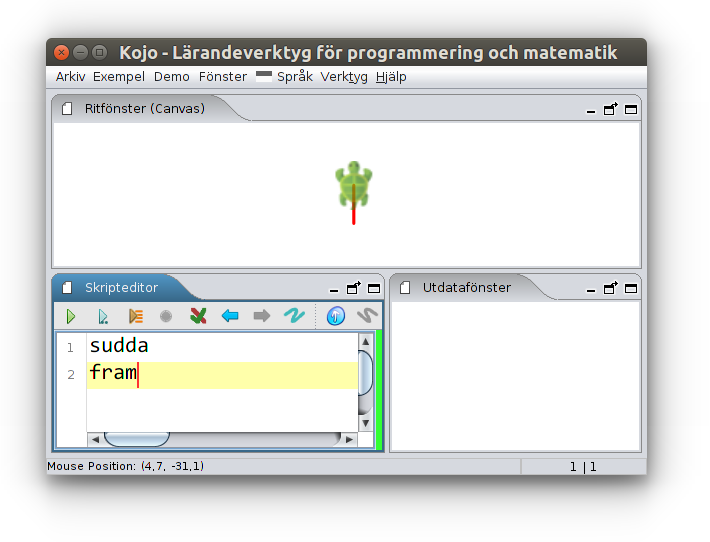
\includegraphics[width=0.8\textwidth]{../img/kojo/kojo.png}
\caption{Den nybörjarvänliga utvecklingsmiljön Kojo för Scala på svenska.}
\label{fig:appendix:ide:kojo}
\end{figure} 

\subsection{Installera Kojo}

Kojo är förinstallerat på LTH:s datorer och körs igång med kommandot \texttt{kojo}. För instruktioner om hur du installerar Kojo på din egen dator se här:\\
\href{http://www.lth.se/programmera/installera/}{lth.se/programmera/installera}

Kojo kräver att \texttt{java} finns på din dator. Eftersom du behöver tillgång till JDK i kursen, är det lika bra att installera hela JDK direkt (och inte bara JRE, så som beskrivs å länken ovan); se vidare hur du gör detta i avsnitt \ref{appendix:compile:install-jdk}. 
%\href{http://www.kogics.net/kojo-download}{www.kogics.net/kojo-download}


\subsection{Använda Kojo}

När du startar Kojo första gången, välj ''Svenska'' i språkmenyn och starta om Kojo. Därefter fungerar grafikfunktionerna på svenska enligt tabell \ref{table:kojo:functions}. När du startat om Kojo inställt på Svenska ser programmet ut ungeför som i figur \ref{fig:appendix:ide:kojo} på sidan \pageref{fig:appendix:ide:kojo}.


Det finns ett antal användbara kortkommando som du hittar i menyerna i Kojo. Undersök speciellt Ctrl+Alt+Mellanslag som ger autokomplettering baserat på det du börjat skriva.


{\small\renewcommand{\arraystretch}{1.45}
\begin{longtable}{@{}p{0.42\textwidth} p{0.55\textwidth}}

\caption{Några av sköldpaddans funktioner. Se även \href{http://lth.se/programmera}{lth.se/programmera}}\label{table:kojo:functions}\\

\emph{Svenska/Engelska} & \emph{Vad händer?}  \\ \hline
%!TEX encoding = UTF-8 Unicode
%!TEX root = ../compendium2.tex

\chapter{Kojo}\label{appendix:kojo}

\section{Vad är Kojo?}

Kojo%
\footnote{\href{https://en.wikipedia.org/wiki/Kojo_(programming_language)}{en.wikipedia.org/wiki/Kojo\_(programming\_language)}}
 är en integrerad utvecklingsmiljö för Scala som är speciellt anpassad för programmeringsundervisning i grundskolan. Kojo används i LTH:s Science Center Vattenhallen för utbildning av grundskolelärare i programmering och vid skolbesök och annan besöksverksamhet, i vilken lärare och studenter vid LTH arbetar som handledare. 
 
 Kojo är öppen källkod och utvecklingsgemenskapen leds av Lalit Pant från Indien. I Kojo finns även lättillgängliga bibliotek som gör tröskeln lägre att programmera rörlig grafik och enkla spel.

Under kursens första laboration använder vi grafikbiblioteket i Kojo för att illustrera grundläggande begrepp, så som sekvens, alternativ, repetition och abstraktion.  


\begin{figure}[H]
\centering
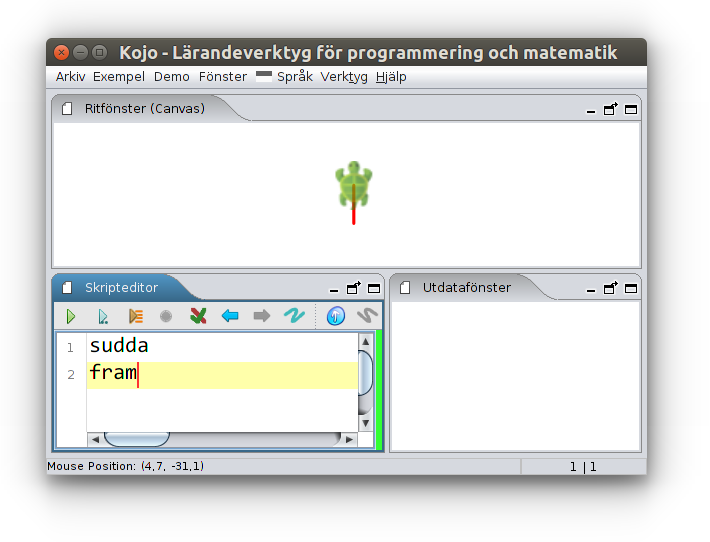
\includegraphics[width=0.8\textwidth]{../img/kojo/kojo.png}
\caption{Den nybörjarvänliga utvecklingsmiljön Kojo för Scala på svenska.}
\label{fig:appendix:ide:kojo}
\end{figure}

\section{Använda grafikbiblioteket i Kojo}\label{appendix:ide:kojo:install}

Kojo bygger på den beprövade pedagogiska idén med sköldpaddsgrafik \Eng{turtle graphics}\footnote{\url{https://en.wikipedia.org/wiki/Turtle_graphics}}, där du skriver program som styr en sköldpadda med en penna under magen. När sköldpaddan rör sig bildas ett streck av valfri färg på skärmen. Beroende på hur du bestämmer att sköldpaddan ska röra sig och vilken färg du bestämmer att pennan ska ha, kan du skapa olika intressanta bilder och samtidigt lära dig om programmeringens grunder.

Under kursens första laboration ska du använda grafikbiblioteket i Kojo tillsammans med editorn VS \code{code} och \code{scala-cli} i terminalen (se appendix \ref{appendix:terminal} och \ref{appendix:compile}). Ladda ner filen \texttt{kojo.scala} från \url{https://cs.lth.se/pgk/kojolib} och spara i en ny katalog med hjälp av din webbläsare, eller via dessa kommandon:

\begin{REPLnonum}
> mkdir w01-kojo
> cd w01-kojo
> curl -o kojolib.scala -sL https://cs.lth.se/pgk/kojolib
\end{REPLnonum}

Nu kan du starta Scala REPL och rita med Kojo så här:

\begin{REPLnonum}
> scala-cli repl .
Welcome to Scala 3.1.2 (17.0.2, Java OpenJDK 64-Bit Server VM).
Type in expressions for evaluation. Or try :help.
                                                                                                                               
scala> fram; höger; fram; vänster

\end{REPLnonum}

Du kan starta VS \code{code} i aktuellt bibliotek så här:
\begin{REPLnonum}
> code .
\end{REPLnonum}

Skriv nedan progam i VS \code{code} och spara det i samma katalog som den tidigare nedladdade filen, under ett nytt valfritt filnamn, t.ex. \code{rita.scala}:

\begin{Code}
@main def rita =
  fram; höger
  fram; vänster
\end{Code}

Kör ditt fristående program med:
\begin{REPLnonum}
> scala-cli run .
\end{REPLnonum}

Du ska nu få upp ett fönster som heter Kojo Canvas med en sköldpadda som ritat två streck. När du stänger fönstret så avslutas programmet. Prova fler sköldpaddsfunktioner enligt tabell \ref{table:kojo:functions}.

I stället för att ladda ned filen \code{kojolib.scala} så kan du placera dess innehåll på lämpligt ställe i ditt program enligt nedan. Observera att raden som börjar med \code{//> using lib} ska vara en enda lång rad utan radbrytningar. Raden med \code{export} gör Kojos kommandon tillgängliga utan prefix:
\begin{CodeSmall}[breaklines=true]
//> using scala "3"
//> using lib "net.kogics:kojo-lib:0.1.1,url=https://github.com/lunduniversity/introprog/releases/download/kojo-lib-0.1.1/kojo-lib-0.1.1.jar"

export net.kogics.kojo.Swedish.*, padda.*, CanvasAPI.*, TurtleAPI.*
\end{CodeSmall}


\noindent Scala-koden för den svenska paddans api finns här: \\
%\href{https://github.com/litan/kojo/blob/master/src/main/scala/net/kogics/kojo/lite/i18n/svInit.scala}{github.com/litan/kojo/blob/master/src/main/scala/net/kogics/kojo/lite/i18n/svInit.scala} \\
\href{https://github.com/litan/kojo-lib/blob/main/src/main/scala/net/kogics/kojo/i18n/Swedish.scala}{github.com/litan/kojo-lib/blob/main/src/main/scala/net/kogics/kojo/i18n/Swedish.scala}


%Kojo kräver (numera) \emph{inte} att \texttt{java} finns på din dator utan kommer med en egen JVM. 
%Eftersom du behöver tillgång till JDK i kursen, är det lika bra att installera hela JDK direkt (och inte bara JRE, så som beskrivs å länken ovan); se vidare hur du gör detta i avsnitt \ref{appendix:compile:install-jdk}.
%\href{http://www.kogics.net/kojo-download}{www.kogics.net/kojo-download}


{\small\renewcommand{\arraystretch}{1.4}
\begin{longtable}{@{}p{0.42\textwidth} p{0.55\textwidth}}

\caption{Ett urval av funktioner i Kojo. Se även \href{http://lth.se/programmera}{lth.se/programmera}}\label{table:kojo:functions}\\

\emph{Svenska/Engelska} & \emph{Vad händer?}  \\ \hline
\code|sudda| \newline \code|clear| & Ritfönstret suddas \\
\code|fram| \newline \code|forward()| & Paddan går framåt 25 steg. \\
\code|fram(100)| \newline \code|forward(100)| & Paddan går framåt 100 steg. \\
\code|höger| \newline \code|right(90)| & Paddan vrider sig 90 grader åt höger. \\
\code|höger(45)| \newline \code|right(45)| & Paddan vrider sig 45 grader åt höger. \\
\code|vänster| \newline \code|left(90)| & Paddan vrider sig 90 grader åt vänster. \\
\code|vänster(45)| \newline \code|left(45)| & Paddan vrider sig 45 grader åt vänster. \\
\code|hoppa| \newline \code|hop| & Paddan hoppar 25 steg utan att rita. \\
\code|hoppa(100)| \newline \code|hop(100)| & Paddan hoppar 100 steg utan att rita. \\
\code|hoppaTill(100, 200)| \newline \code|jumpTo(100, 200)| & Paddan hoppar till läget (100, 200) utan att rita. \\
\code|gåTill(100, 200)| \newline \code|moveTo(100, 200)| & Paddan vrider sig och går till läget (100, 200). \\
\code|hem| \newline \code|home| & Paddan går tillbaka till utgångsläget (0, 0). \\
\code|öster| \newline \code|setHeading(0)| & Paddan vrider sig så att nosen pekar åt höger. \\
\code|väster| \newline \code|setHeading(180)| & Paddan vrider sig så att nosen pekar åt vänster. \\
\code|norr| \newline \code|setHeading(90)| & Paddan vrider sig så att nosen pekar uppåt. \\
\code|söder| \newline \code|setHeading(-90)  | & Paddan vrider sig så att nosen pekar neråt. \\
\code|mot(100,200)| \newline \code|towards(100, 200)| & Paddan vrider sig så att nosen pekar mot läget (100, 200) \\
\code|sättVinkel(90)| \newline \code|setHeading(90)| & Paddan vrider nosen till vinkeln 90 grader. \\
\code|vinkel| \newline \code|heading| & Ger vinkelvärdet dit paddans nos pekar. \\
\code|sakta(5000)| \newline \code|setAnimationDelay(5000) | & Gör så att paddan ritar jättesakta. \\
\code|suddaUtdata| \newline \code|clearOutput| & Utdatafönstret suddas. \\
\code|utdata("hej")| \newline \code|println("hej")| & Skriver texten \texttt{hej} i utdatafönstret. \\
\code|val t = indata("Skriv")| \newline \code|val t = readln("Skriv:")| & Väntar på inmatning efter ledtexten \texttt{Skriv} och sparar den inmatade texten i t.  \\
\code|textstorlek(100)| \newline \code|setPenFontSize(100)| & Paddan skriver med jättestor text nästa gång du gör skriv. \\
\code|båge(100, 90)| \newline \code|arc(100, 90)| & Paddan ritar en båge med radie 100 och vinkel 90. \\
\code|cirkel(100)| \newline \code|circle(radie)| & Paddan ritar en cirkel med radie 100. \\
\code|synlig| \newline \code|visible| & Paddan blir synlig. \\
\code|osynlig| \newline \code|invisible| & Paddan blir osynlig. \\
\code|läge.x| \newline \code|position.x| & Ger paddans x-läge \\
\code|läge.y| \newline \code|position.y| & Ger paddans y-läge \\
\code|pennaNer| \newline \code|penDown| & Sätter ner paddans penna så att den ritar när den går. \\
\code|pennaUpp| \newline \code|penUp| & Lyfter upp paddans penna så att den INTE ritar när den går. \\
\code|pennanÄrNere| \newline \code|penIsDown| & Kollar om pennan är nere eller inte. \\
\code|färg(rosa)| \newline \code|setPenColor(pink)| & Sätter pennans färg till rosa. \\
\code|fyll(lila)| \newline \code|setFillColor(purple)| & Sätter ifyllnadsfärgen till lila. \\
\code|fyll(genomskinlig)| \newline \code|setFillColor(noColor)| & Gör så att paddan inte fyller i något när den ritar. \\
\code|bredd(20)| \newline \code|setPenThickness(20)| & Gör så att pennan får bredden 20. \\
\code|sparaStil| \newline \code|saveStyle| & Sparar pennans färg, bredd och fyllfärg. \\
\code|laddaStil| \newline \code|restoreStyle| & Laddar tidigare sparad färg, bredd och fyllfärg. \\
\code|sparaLägeRiktning| \newline \code|savePosHe| & Sparar pennans läge och riktning \\
\code|laddaLägeRiktning| \newline \code|restorePosHe| & Laddar tidigare sparad riktning och läge \\
\code|siktePå| \newline \code|beamsOn| & Sätter på siktet. \\
\code|sikteAv| \newline \code|beamsOff| & Stänger av siktet. \\
\code|bakgrund(svart)| \newline \code|setBackground(black)| & Bakgrundsfärgen blir svart. \\
\code|bakgrund2(grön,gul)| \newline \code|setBackgroundV(green, yellow)| & Bakgrund med övergång från grönt till gult. \\
\code|upprepa(4){fram; höger}| \newline \code|repeat(4){forward; right}| & Paddan går fram och svänger höger 4 gånger. \\
\code|avrunda(3.99)| & Avrundar 3.99 till 4.0 \\
\code|slumptal(100)| & Ger ett slumptal mellan 0 och 99. \\
\code|slumptalMedDecimaler(100)| & Ger ett slumptal mellan 0 och 99.99999999 \\
\code|systemtid| & Ger nuvarande systemklocka i sekunder. \\
\code|räknaTill(5000)| & Kollar hur lång tid det tar för din dator att räkna till 5000. \\


\end{longtable}
}%end small


\section{Kojo Desktop}

Kojo finns som fristående skrivbordsapplikation, kallad Kojo Desktop. Kojo Desktop innehåller en egen editor med syntaxfärgning för Scala, men fungerar ännu så länge bara för Scala 2. En av de synligaste skillnaderna mellan Scala 2 och Scala 3 är att klammerparenteser vid flerradiga funktioner är nödvändiga i Scala 2, medan Scala 3 har valfria klammerparenteser. Så om du använder Kojo Desktop behöver du komma ihåg att omgärda sekvenser av rader som hör ihop med \code|{| och \code|}|. 

Kojo Desktop är förinstallerat på LTH:s datorer och körs igång med terminalkommandot \texttt{kojo} eller via applikationsmenyn.  För instruktioner om hur du installerar Kojo Desktop på din egen dator se här: \href{http://www.lth.se/programmera/installera/}{lth.se/programmera/installera}

När du startar Kojo första gången, välj ''Svenska'' i språkmenyn och starta om Kojo. Därefter fungerar grafikfunktionerna på svenska enligt tabell \ref{table:kojo:functions}. När du startat om Kojo inställt på svenska ser programmet ut ungefär som i figur \ref{fig:appendix:ide:kojo} på sidan \pageref{fig:appendix:ide:kojo}.

Det finns ett antal användbara kortkommando som du hittar i menyerna i Kojo Desktop. Undersök speciellt Ctrl+Alt+Mellanslag som ger autokomplettering baserat på det du börjat skriva.

\section{Kojo i Webbläsaren}

En begränsad variant av Kojo finns tillgänglig för programmering direkt i din webbläsare här: \url{http://kojo.lu.se/}

När du trycker på play-knappen så kompileras din kod på en server till Javascript via ScalaJS och därefter körs Javascript-koden i din webbläsare. 
Kojo på webben är också ännu så länge begränsad till Scala 2 och kräver att du omgärdar sekvenser av rader som hör ihop med \code|{| och \code|}|.


\section{Mer om Kojo}

I detta dokument finns en enkel introduktion till Kojo: \\ ''Introduction to Kojo'' \url{http://www.kogics.net/kojo-ebooks#intro}


\hline
\end{longtable}
}%end small

\noindent Scala-koden för den svenska paddans api finns här: \\
\href{https://bitbucket.org/lalit_pant/kojo/src/tip/src/main/scala/net/kogics/kojo/lite/i18n/svInit.scala}{bitbucket.org/lalit\_pant/kojo/src/tip/src/main/scala/net/kogics/\\kojo/lite/i18n/svInit.scala}




\newpage

\section{Eclipse och ScalaIDE}\label{appendix:ide:eclipse}

Eclipse%
\footnote{\href{https://en.wikipedia.org/wiki/Eclipse_(software)}{en.wikipedia.org/wiki/Eclipse\_(software)}}
är en professionell IDE som stödjer många olika programmeringsspråk. Eclipse är skriven i Java och bygger vidare på ett utvecklingsprojekt som initierades av IBM. Eclipse är ett fritt och öppet projekt som numera kontrolleras av en oberoende stiftelse.

Till Eclipse finns en insticksmodul \Eng{plug-in} som kallas ScalaIDE och erbjuder stöd för Scala med tillhörande standardbibliotek.

Eclipse är en omfattande och avancerad programmeringsmiljö med många funktioner och inställningar. Det finns även en omfattande uppsättning insticksmoduler och tilläggsprogram som underlättar utveckling av t.ex. webbprogram, databaser och mycket annat. 

I detta avsnitt ges länkar till installation samt tips om hur du kommer igång med att använda Eclipse och ScalaIDE. Det går ganska snabbt att lära sig grunderna, men det kräven en viss ansträngning att lära sig de mer avancerade funktionerna. Det finns omfattande resurser på nätet som hjälper dig vidare. 


\subsection{Installera Eclipse Mars och ScalaIDE}\label{appendix:ide:eclipse:install}

Eclipse med ScalaIDE är förinstallerat på LTH:s datorer och startas med kommandot \texttt{scalaide} i ett terminalfönster.

ScalaIDE fungerar med Eclipse-versionerna \textit{Luna} och \textit{Mars} (men i skrivande stund fungerar ScalaIDE ännu \textit{inte} med den allra senaste versionen kallad \textit{Neon}). 

För att installera ScalaIDE på din egen dator, följ nedan instruktioner: 

\begin{enumerate}
\item Kontrollera enligt avsnitt \ref{appendix:compile:check-jdk} att du har \texttt{java} installerat och installera vid behov JDK enligt avsnitt \ref{appendix:compile:install-jdk}.

\item Installera Eclipse version \textbf{Mars}, varianten för \textbf{Java Developers} som återfinns på denna sida: \\ \url{https://www.eclipse.org/downloads/packages/release/Mars/2} \\ som är den \textit{andra} varianten i listan (alltså inte Java EE). Följ dessa steg:
\begin{enumerate}
\item Klicka på den \textbf{64-bit}-variant som passar ditt operativsystem.
\item Filen som laddas ner heter något som liknar (beroende på OS): \\ \texttt{eclipse-java-mars-2-win32-x86\_64.zip} 
\\ Det kan ta lång tid att ladda ner filen som är på ca 170MB. Om du klickar på \textit{''select a mirror''} kan du välja en svensk sajt för att ladda ner snabbare. 

\item Dubbelklicka på filen för att packa upp den, vilket kan ta många minuter. Du får, när upppackningen är klar, ett bibliotek med en fungerande Eclipse-installation som du kan placera var du vill. Kör du Windows, lägg den förslagsvis här:\\ 
\code|C:\eclipse\eclipse-java-mars-2-win32-x86_64|

\item för Ubuntu Linux finns kompletterande installationsanvisningar här, som ger dig en ikon i app-menyn m.m.: 
\\ \url{http://askubuntu.com/questions/26632/how-to-install-eclipse}
\end{enumerate}

\item Installera Scala IDE inifrån%
\footnote{Det finns på ScalaIDE-hemsidan möjlighet att ladda ner en Eclipse-variant med färdiginstallerad ScalaIDE-plugin, men då får du i skrivande stund den gamla versionen Eclipse \textit{Luna}, varför du rekommenderas att, enligt instruktionerna här, själv installera ScalaIDE inifrån Eclipse \textit{Mars}, som är den senaste Eclipse-versionen för vilken ScalaIDE fungerar.}
 Eclipse enligt nedan steg:
\begin{enumerate}
\item Starta Eclipse, t.ex. genom att köra igång den exekverbara filen som ligger i underbiblioteket \texttt{eclipse}, i Windows heter den \texttt{eclipse.exe} medan den exekverbara filen i Linux heter \texttt{eclipse} utan filändelse.

\item Välj i frågerutan som dyker upp, någon plats för \textit{workspace} (kvittar vilken just nu, kan ändras senare).

\item Klicka på menyn \textit{Help} $\rightarrow$ \textit{Install new software}.

\item Klicka på \textit{Add}-knappen till höger och skriv: \\ \textit{''ScalaIDE for Scala 2.11''} i \textit{Name}-fältet och ange denna adress i \textit{Location}-fältet: \\
  {\small\mbox{\url{http://download.scala-ide.org/sdk/lithium/e44/scala211/stable/site}}} \\
  och klicka \textit{OK}.
  
\item Du får nu upp en lista med alternativ. Kryssa för alternativet
\\ {\frame{\checkmark}}~~\textit{Scala IDE for Eclipse} \\ och klicka \textit{Next} och sedan \textit{Next} igen och acceptera licensvillkoren och klicka \textit{Finish}.

\item Låt installationen ta sin tid och starta sedan om Eclipse när installationen är färdig. 

\item När Eclipse är igång igen visas en dialog som föreslår att du ska köra \textit{Setup Diagnostics}. Gör detta och välj \textit{Use recommended default settings}. Ändra även i filen \textbf{eclipse.ini} för höja den övre minnesgränsen. Det gör du genom att ändra på den rad i filen som börjar med \texttt{-Xmx}. Hur mycket du ska tillåta som max beror på hur mycket minne du har, men ge minst 1 gigabyte för smidig körning, genom att skriva så här på relevant rad i filen \textbf{eclipse.ini}: \\
\texttt{-Xmx1G } \\


\item Kompletterande information finns här, inklusive en video som visar installationsproceduren och hur man kommer igång med ett ''hello world''-program: \\ \url{http://scala-ide.org/download/current.html}


\end{enumerate}


\end{enumerate}

\noindent I nästa avsnitt beskrivs några rekommenderade anpassningar som du kan göra bland de omfattande inställningsmöjligheterna för Eclipse.

\newpage

\subsection{Anpassa Eclipse och ScalaIDE}\label{subsection:appendix:ide:eclipse:tweaks}

\newcommand\Menu[1]{\textit{#1}}
\newcommand\MenuArrow[1]{\Menu{#1}~$\rightarrow$~}
\newcommand\FramedCheckmark[1]{~\frame{\checkmark}~~\textbf{#1}}
\newcommand\FramedUnchecked[1]{$\Box$~\textbf{#1}}
\newcommand\Button[1]{\fbox{\textbf{#1}}}
\newcommand\EclipsePrefs{\MenuArrow{Window}\MenuArrow{Preferences}}
\newcommand\EclipsePrefsGeneral{\EclipsePrefs\MenuArrow{General}}


Förutom maxminneshöjningen i filen \texttt{eclipse.ini}, som finns i installationskatalogen för Eclipse, till minst \texttt{-Xmx1G } (se föregående avsnitt), är det bra att göra några ytterligare anpassningar av Eclipse och ScalaIDE för att få en snabbare och smidigare utvecklingsmiljö. Du hittar inställningarna i menyn \EclipsePrefs ... uppe till höger i Eclipse-fönstret.



\begin{enumerate}
\item \EclipsePrefsGeneral 
\\ Markera \FramedCheckmark{Show Heap Status} så får du se minnesanvändningen i en liten ruta i nederdelen av fönstret, vilket hjälper dig att upptäcka om minnesbegränsningen i filen \texttt{eclipse.ini} är en flaskhals vid stora projekt och många öppna fönster. Klicka sedan \Button{Apply} längst ner.

\item \label{item:scala-perspective} \EclipsePrefsGeneral\MenuArrow{Editors}\MenuArrow{Perspective}  
\\ Markera \textit{Scala} i listan med perspektiv och klicka på knappen 
 \\ \Button{Make default} till höger och sedan på knappen \Button{Apply} längst ner.

\item \EclipsePrefsGeneral\MenuArrow{Editors}\MenuArrow{TextEditors}
\\ Markera \FramedCheckmark{Insert spaces for tabs} så att du slipper specialtecken som kan tolkas olika av olika editorer. Klicka sedan \Button{Apply} längst ner.

\item \EclipsePrefsGeneral\MenuArrow{Editors}\MenuArrow{TextEditors}
\\ \MenuArrow{Spelling} Avmarkera \FramedUnchecked{Enable spell checking} för att slippa att svenska namn och svenska kommentarer markeras som felstavade. Om du senare jobbar med ett projekt helt på engelska, kan du med fördel markera denna kryssruta igen. Klicka sedan \Button{Apply} längst ner.

\item \EclipsePrefsGeneral\MenuArrow{Editors}\MenuArrow{Webbrowser}
\\ Markera \FramedCheckmark{Use external web browser} för att köra din vanliga webbläsare när du klickar på länkar. Klicka sedan \Button{Apply} längst ner.
  
\item  \EclipsePrefs\MenuArrow{Scala}\MenuArrow{Compile}
\\ I fliken \textbf{Standard} markera dessa kryssrutor för att få extra varningar: \\
\begin{tabular}{l @{}l @{}l}
\textit{deprecation} & \FramedCheckmark{} & varnar vid användning av föråldrad kod som snart utgår \\
\textit{feature}     & \FramedCheckmark{} & påminner om import vid användning av avancerad kod  \\
\textit{unchecked}   & \FramedCheckmark{} & ger tips vid speciella problem med generiska typer \\
\end{tabular}\\
och klicka sedan på knappen \Button{Apply} längst ner.

\item \EclipsePrefs\MenuArrow{Java}\MenuArrow{Compiler}\MenuArrow{Errors/Warnings}
\\ Veckla ut listan \textbf{Potential programming problems} och sätt \textbf{Resource leak} till alternativet \textbf{Ignore}, så slipper du varningar vid användning \jcode{Scanner} i Java. Klicka sedan \Button{Apply} längst ner.

\end{enumerate}

\noindent Ovan anpassningar är rekommenderade men inte nödvändiga och du kan gärna välja att göra andra anpassningar som passar just dig. Skriv då gärna ner vilken inställning du ändrat, så att du hittar tillbaka om du ångrar dig. 

Du hittar tips om fler inställningar för att anpassa ScalaIDE här: \\
\url{http://scala-ide.org/docs/current-user-doc/advancedsetup}



\subsection{Använda Eclipse och ScalaIDE}\label{appendix:ide:eclipse:use}

Ett grundläggande koncept i Eclipse är \textbf{workspace}. Ett workspace utgör ett arbetsområde kopplat till en katalog i ditt filsystem där du kan arbeta med ett eller flera \textbf{projekt}. Ett projekt innehåller i sin tur dina källkodsfiler och klassfiler etc. i en specifik katalogstruktur som Eclipse skapar när du editerar, kompilerar och kör dina projekt. 

\subsubsection{Starta och välja workspace}\label{subsubsection:start:eclipse}

När du startar Eclipse måste du välja vilket workspace du vill använda innan du kommer vidare. När du kör igång Eclipse första gången, klicka OK enligt det förslag som ges. Du kan senare växla workspace genom menyn \MenuArrow{File}\Menu{Switch Workspace}. Om katalogen du anger inte redan finns, kommer den att skapas och initieras med de filer Eclipse behöver.

I figur \ref{fig:appendix:eclipse:welcome} visas välkomstfliken i Eclipse med sina länkar till funktionsöversikt och olika handledningar. Stäng välkomstfliken genom att klicka på flikens kryss eller på ikonen \textit{Workbench}. Då kommer du vidare till den normala arbetsytan i Eclipse. Du kan få tillbaka välkomstfliken igen via menyn \MenuArrow{Help}\Menu{Welcome}. 

\begin{figure}[H]
\centering
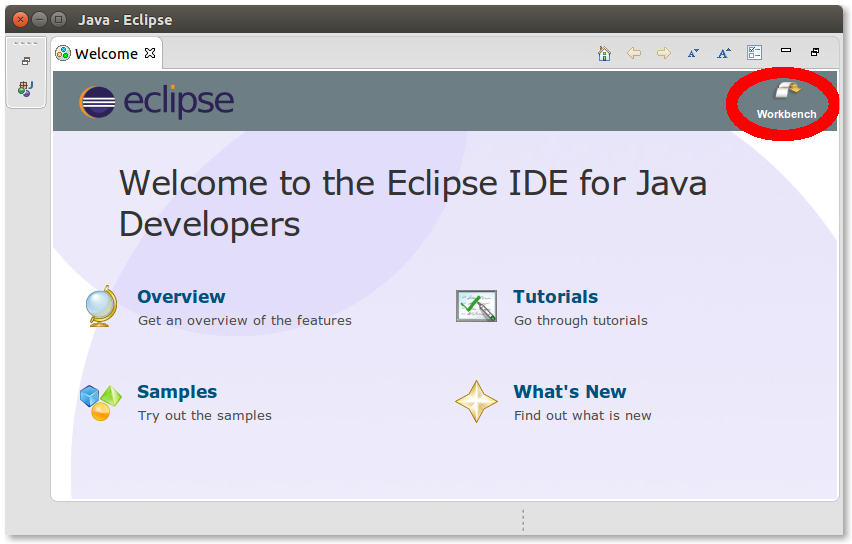
\includegraphics[width=1.0\textwidth]{../img/eclipse/eclipse-welcome.png}
\caption{Välkomstfliken för Eclipse, som nås via menyn \MenuArrow{Help}\Menu{Welcome}. Gå vidare genom att klicka på \textit{Workbench}.}
\label{fig:appendix:eclipse:welcome}
\end{figure}

\subsubsection{Välja perspektiv och visa olika vyer}

Eclipse-fönstret kan innehålla många underfönster i olika flikar, så kallade \textbf{views} eller vyer, som kan arrangeras på olika vis efter hur du vill ha dem. Vilka vyer som syns och hur de placeras beror på vilket s.k. \textbf{perspective} som är aktivt.  Figur \ref{fig:appendix:eclipse:open-perspective} visar arbetsytan med olika vyer i Java-perspektivet. 

Du kan byta till Scala-perspektivet genom att trycka på 
\includegraphics[scale=0.75]{../img/eclipse/eclipse-perspective-button.png} eller genom menyn \MenuArrow{Window}\MenuArrow{Perspective}\MenuArrow{Open Perspective}\MenuArrow{Other...}\Menu{Scala}.
Du kan anpassa inställningarna så att Scala blir \textit{default perspective}, se steg \ref{item:scala-perspective} i avsnitt \ref{subsection:appendix:ide:eclipse:tweaks} på sidan \pageref{subsection:appendix:ide:eclipse:tweaks}.

Stäng vyerna \textit{Task List} och \textit{Outline} om du vill ha mer plats till de övriga vyerna för paketnavigering, editering och utdata. Du kan öppna stängda vyer igen genom menyn \MenuArrow{Window}\Menu{Show View}. 

\begin{figure}
\centering
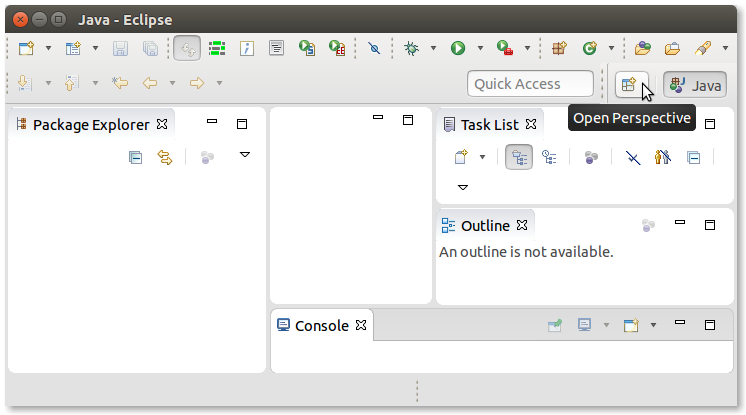
\includegraphics[width=1.0\textwidth]{../img/eclipse/eclipse-open-perspective.png}
\caption{Arbetsytan i Eclipse. Du kan växla mellan Scala- och Java-perspektivet genom att klicka på perspektivvalsknappen.}
\label{fig:appendix:eclipse:open-perspective}
\end{figure}

\subsubsection{Hello World}\label{subsubsection:eclipse:hello-world}

Efter att du öppnat Eclipse med ScalaIDE i ett tomt workspace och valt Scala-perspektivet enligt föregående avsnitt, kan du skapa ditt första projekt med ett \textit{''Hello World''}-program enligt stegen nedan.

\begin{enumerate}
\item Högerklicka i \Menu{Package Explorer} och välj \MenuArrow{New}\Menu{Scala Project}, varefter en dialogruta visas. 

\item Fyll i namnet \texttt{hello} i fältet \Menu{Project Name} och klicka \Button{Finish}.

\item Högerklicka igen i \Menu{Package Explorer} och välj \MenuArrow{New}\Menu{Scala Object}, varefter en ny dialogruta visas. 

\item Fyll i namnet \texttt{hi} i fältet \Menu{Project Name} och klicka \Button{Finish}.

\item Du får nu i editorvyn ett kodskellet med \code{object hi}.

\item Börja skriv \code{main} som visas i figur \ref{fig:appendix:eclipse:complete-main} och tryck Ctrl+Mellanslag för att aktivera kodkomplettering \Eng{code completion}. Då får du upp en lista med alternativ. Välj det översta alternativet \texttt{main} varefter ett kodskellet med en main-metod klistras in automatiskt i din kod.

\begin{figure}
\centering
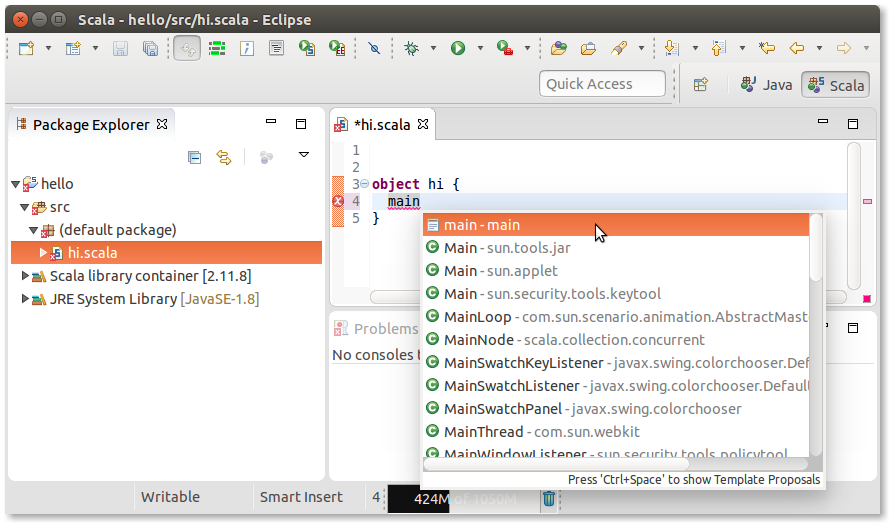
\includegraphics[width=1.0\textwidth]{../img/eclipse/eclipse-complete-main.png}
\caption{Aktivera kodkomplettering med Ctrl+Mellanslag efter ordet \code{main}.}
\label{fig:appendix:eclipse:complete-main}
\end{figure}

\item Fyll i lämplig utskriftstext i ett \code{println}-anrop så att din \code{main}-metod blir så som visas i editorfliken i figur \ref{fig:appendix:eclipse:hello-world}.

\begin{figure}[H]
\centering
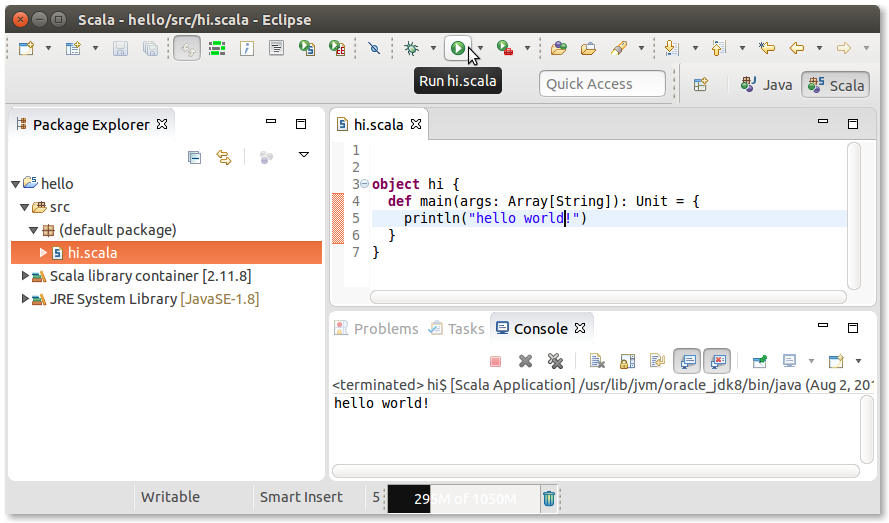
\includegraphics[width=1.0\textwidth]{../img/eclipse/eclipse-hello-world.png}
\caption{Skriv klart \code{main}-metoden och kör ditt program med play-knappen.}
\label{fig:appendix:eclipse:hello-world}
\end{figure}

\item Kör ditt program genom att trycka på den gröna play-knappen, som muspekaren i figur \ref{fig:appendix:eclipse:hello-world} pekar på. Du kan också trycka F11 för att köra igång din app, efter att du vid första körningen i dialogen \textit{Select Preferred Launcher} markerat  \FramedCheckmark{Use configuration specific settings} och valt alternativet \textit{Scala Application (new debugger) Launcher}. 

\end{enumerate}




\subsubsection{Ladda ner kursens workspace och importera projekt till labbarna}

Det finns en zip-fil med ett workspace med projekt för flera av kursens laborationer som du kan ladda ner och importera i Eclipse. Följ stegen nedan.

\begin{enumerate}
\item Ladda ner kursens workspace här: \url{http://cs.lth.se/pgk/ws}

\item Packa upp filen på lämpligt ställe.

\item Starta Eclipse med ScalaIDE-plugin (se startinstruktioner på sidan \pageref{subsubsection:start:eclipse}). 

\item Växla workspace till biblioteket du nyss packade upp, ungefär som i figur \ref{fig:eclipse:ide:open} och klicka \Button{OK}.
\begin{figure}[H]
\centering
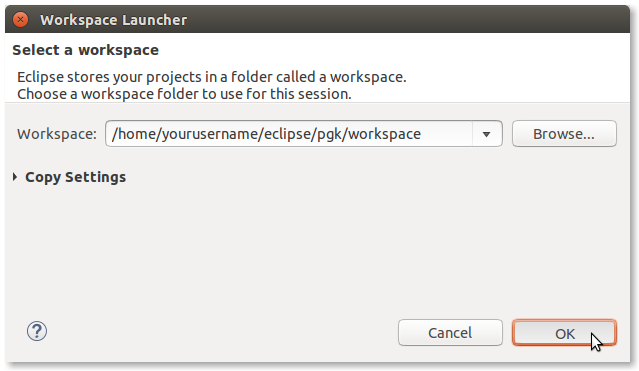
\includegraphics[width=1.0\textwidth]{../img/eclipse/eclipse-select-workspace.png}
\caption {Öppna kursens workspace genom att bläddra till biblioteket där du packade upp filen som du laddat ned från: \url{http://cs.lth.se/pgk/ws} }
\label{fig:eclipse:ide:open}
\end{figure}

\item Stäng välkomstfliken för att komma vidare till workbench (se figur \ref{fig:appendix:eclipse:welcome} på sidan \pageref{fig:appendix:eclipse:welcome}). Det ser då ut ungefär som i figur~\ref{fig:appendix:eclipse:open-perspective} på sidan \pageref{fig:appendix:eclipse:open-perspective}. Det syns ännu inget i \textit{Package Explorer} då vi ännu inte importerat något projekt. 

\item Innan du går vidare, säkerställ att du har Scala-perspektivet aktiverast. Du kan växla till Scala-perspektivet genom att trycka på \includegraphics[scale=0.75]{../img/eclipse/eclipse-perspective-button.png} eller genom menyn \MenuArrow{Window}\MenuArrow{Perspective}\MenuArrow{Open Perspective}\MenuArrow{Other...}\Menu{Scala}.
Du kan anpassa inställningarna så att Scala blir \textit{default perspective}, se steg \ref{item:scala-perspective} i avsnitt \ref{subsection:appendix:ide:eclipse:tweaks} på sidan \pageref{subsection:appendix:ide:eclipse:tweaks}.


\item Högerklicka i \textit{Package Explorer} och välj \Menu{Import...}, se Fig.~\ref{fig:eclipse:import}, eller välj menyn \MenuArrow{File}\Menu{Import...}. 

\begin{figure}[H]
\centering
\includegraphics[width=1.0\textwidth]{../img/eclipse/eclipse-import.png} 

\caption {Välj \Menu{Import}-menyn för att importera existerande projekt.}
\label{fig:eclipse:import}
\end{figure}

\item Nu öppnas \Menu{Import}-dialogen som visas i figur \ref{fig:eclipse:import-existing}. Öppna mappen \Menu{General}, markera \textbf{Existing Projects into Workspace} och klicka \Button{Next}.



\begin{figure}[H]
\centering
\includegraphics[width=0.75\textwidth]{../img/eclipse/eclipse-import-existing.png} 

\caption {Välj att importera existerande projekt under \Menu{General}.}
\label{fig:eclipse:import-existing}
\end{figure}


\begin{figure}[H]
\centering
\includegraphics[width=1.0\textwidth]{../img/eclipse/eclipse-import-projects.png} 

\caption {Välj \FramedCheckmark{Select Root Directory} och klicka \Button{Browse}.}
\label{fig:eclipse:import-projects}
\end{figure}


\item Nu kommer ytterligare ett dialogfönster som visas i figure \ref{fig:eclipse:import-projects}. Med \FramedCheckmark{Select Root Directory} markerad kan du klicka \Button{Browse} för att ange workspace-mappen i ännu en dialog där du bara ska trycka \Button{Ok} utan att välja underbibliotek till workspace. När det är klart ska det se ut som i figur \ref{fig:eclipse:import-projects} där alla Eclipse-projekt \FramedCheckmark{cslib}, \FramedCheckmark{w04\_pirates}, etc. är markerade. Klicka sedan \Button{Finish}.

\item Följ ''Hello World''-instruktionerna på sidan \pageref{subsubsection:eclipse:hello-world} och skapa programmet som visas i figure \ref{fig:eclipse:pirates-hi}, genom att veckla ut projektet \textbf{w04\_pirates}, markera och högerklicka på paketet \textbf{priates}, och välja \MenuArrow{New}\Menu{Scala Object}.

\begin{figure}[H]
\centering
\includegraphics[width=1.0\textwidth]{../img/eclipse/eclipse-pirates-hi.png} 

\caption {Skapa ett \MenuArrow{New}\Menu{Scala Object} med kod enligt bilden.}
\label{fig:eclipse:pirates-hi}
\end{figure}


\end{enumerate}



\newpage

\section{IntelliJ IDEA}\label{appendix:ide:intellij}

IntelliJ IDEA%
\footnote{\href{https://en.wikipedia.org/wiki/IntelliJ_IDEA}{en.wikipedia.org/wiki/IntelliJ\_IDEA}}
 är en professionell IDE som stödjer många olika programmeringsspråk. IntelliJ är skriven i Java och utvecklas av det tjeckiska företaget JetBrains. 

IntelliJ IDEA finns i två varianter: en gratis gemenskapsvariant med öppenkällkodslicens \Eng{Community edition}, samt en betalvariant med stängd källkod och support-tjänster.


Till IntelliJ IDEA finns en insticksmodul \Eng{plug-in} som erbjuder stöd för Scala med tillhörande standardbibliotek..

IntelliJ IDEA är en omfattande och avancerad programmeringsmiljö med många funktioner och inställningar. Det finns även en omfattande uppsättning insticksmoduler och tilläggsprogram som underlättar utveckling av t.ex. webbprogram, databaser och mycket annat. 

I detta avsnitt ges länkar till installation samt tips om hur du kommer igång med att använda IntelliJ IDEA med Scala. Det går ganska snabbt att lära sig grunderna, men det kräven en viss ansträngning att lära sig de mer avancerade funktionerna. Det finns omfattande resurser på nätet som hjälper dig vidare. 

Google tillkännagav 2013 att företaget övergår från Eclipse till IntelliJ som den officiellt understödda utvecklingsmiljön för Android och 2014 lanserades utvecklingsmiljön AndroidStudio%
\footnote {\href{https://en.wikipedia.org/wiki/Android_Studio}{en.wikipedia.org/wiki/Android\_Studio}}
 som bygger vidare på IntelliJ. 

\subsection{Installera IntelliJ med Scala}\label{appendix:ide:intellij:install}

IntelliJ med Scala-plug-in är förinstallerat på LTH:s datorer och startas med kommandot \texttt{intellij} i ett terminalfönster.

\TODO Beskriv hur man installerar IntelliJ med Scala

\subsection{Använda IntelliJ}\label{appendix:ide:intellij:use}

\TODO 

%%!TEX encoding = UTF-8 Unicode
%!TEX root = ../compendium2.tex

\chapter{Skapa webb-appar med ScalaJS}\label{appendix:scalajs}

\begin{itemize}
\item Lär mer här: \url{http://scala-js.org/}
\item Exempel: \url{https://github.com/bjornregnell/kapten-alloc-web}
\item Exempel på konfiguration av bygge:
\begin{itemize}
\item Lägg in plugin för ScalaJS i \texttt{project/plugins.sbt}: \\\url{https://github.com/bjornregnell/kapten-alloc-web/blob/master/project/plugins.sbt}
\item Lägg till ScalaJS-biblioteket i \texttt{build.sbt}: \\\url{https://github.com/bjornregnell/kapten-alloc-web/blob/master/build.sbt} 
\item Lägg till \texttt{<script>}-tag i \code{index.html}: \\\url{https://github.com/bjornregnell/kapten-alloc-web/blob/master/index.html} 
\item Skapa webbappen med \code{sbt fastLinkJS} vid utveckling och när klar så skapa optimerad app med \code{sbt fullLinkJS}
\end{itemize}
\end{itemize} %TODO!!
%%!TEX encoding = UTF-8 Unicode
%!TEX root = ../compendium2.tex

\chapter{Skapa Android-appar i Scala}\label{appendix:scala-android}

\TODO

\noindent Läs först appendix \ref{appendix:build}

\begin{itemize}
\item \url{http://scala-android.org/}
\end{itemize} %TODO!!
%%!TEX encoding = UTF-8 Unicode
%!TEX root = ../compendium.tex

\chapter{Virtuell maskin}\label{appendix:vbox}

\section{Vad är en virtuell maskin?}

Du kan köra alla kursens verktyg i en så kallad virtuell maskin (vm). Det är ett enkelt och säkert sätt att installera ett nytt operativsystem i en ''sandlåda'' som inte påverkar din dators ursprungliga operativsystem. 

\section{Installera kursens vm}
Det finns en virtuell maskin förberedd med alla verktyg som du behöver förinstallerade. Gör så här:
\begin{enumerate}
\item     Installera VirtualBox v5 här: \\ \url{https://www.virtualbox.org/wiki/Downloads}
\item     Ladda ner filen vbox.zip här: \\ \url{http://fileadmin.cs.lth.se/pgk/vbox.zip} \\ OBS! Då filen är på nästan 4GB kan nedladdningen ta mycket lång tid.
\item     Packa upp filen vbox.zip i biblioteket "VirtualBox VMs" som du fick i din hemkatalog när du installerade VirtualBox. Du får då 3 filer som heter något med "introprog-ubuntu-64bit".
\item     Kolla med hjälp av denna sida: \\ \url{https://md5file.com/calculator} \\ så att filen "introprog-ubuntu-64bit.vdi" har denna sha256-cheksumma: \\ --- ska-stå-checksumma-här-sen ---
\item     Öppna VirtualBox och lägg till maskinen introprog-ubuntu-64bit genom menyn ''add''.
\item     Starta maskinen.
\item     Öppna ett terminalfönster och skriv scala och du är igång och kan göra första övningen!
\end{enumerate}

\section{Vad innehåller kursens vm?}

Den virtuella maskinen kör Xubuntu 14.04 med fönstermiljön XFCE, vilket är samma miljö som E-husets linuxdatorer kör. 

I den virtuella maskinen finns detta förinstallerat:

\begin{itemize}
\item Java JDK 8
\item Scala 2.11.8
\item Kojo 2.4.08
\item Eclipse Mars.2 med ScalaIDE 4.3
\item gedit med syntaxfärgning för Scala och Java
\item git
\item sbt
\item Ammonite REPL
\end{itemize}  %TODO!!

\part{Lösningar}

\setcounter{chapter}{11} %next is L in \Alph
\chapter{Lösningar till övningarna}\label{chapter:solutions}
\setcounter{section}{7}

\PreSolutionfalse

\let\QUESTBEGIN\ifPreSolution  % to mark formatting and numbering of exercises
\let\SOLUTION\else  % to mark solutions in the same file as questions
\let\QUESTEND\fi    % to mark end of exercise


%!TEX encoding = UTF-8 Unicode
%!TEX root = ../exercises.tex

\ifPreSolution

\Exercise{\ExeWeekEIGHT}\label{exe:W08}

\begin{Goals}
\item Kunna skapa och använda matriser med nästlade strukturer av \code{Vector}.
\item Kunna iterera över elementen i en matris med nästlade \code{for}-satser och \code{for}-\code{yield}-uttryck, samt nästlad applicering av \code{map} respektive \code{foreach}.
\item Kunna skapa och använda funktioner som tar matriser som parametrar.
\item Kunna skapa en enkel generisk klass och enkla generiska funktioner med hjälp av en typparameter.
\item Kunna beskriva skillnader och likheter mellan Scala och Java vad gäller indexering och iterering i matriser implementerade med nästlade arrayer.
%\item Kunna skapa och använda matriser med hjälp inbyggda arrayer i Java.
%\item Kunna använda nästlade \code{for}-satser i Java för att iterera över elementen i en matris.
\end{Goals}

\begin{Preparations}
\item \StudyTheory{08}
\end{Preparations}

\BasicTasks

\else

\ExerciseSolution{\ExeWeekEIGHT}

\BasicTasks

\fi



\WHAT{Para ihop begrepp med beskrivning.}

\QUESTBEGIN

\Task \what

\vspace{1em}\noindent Koppla varje begrepp med den (förenklade) beskrivning som passar bäst:

\begin{ConceptConnections}
  matris & 1 & & A & konkret typ, binds till typparameter vid kompilering \\ 
  generisk & 2 & & B & indexerbar datastruktur i två dimensioner \\ 
  typargument & 3 & & C & har abstrakt typparameter, typen är generell \\ 
  typhärledning & 4 & & D & kompilatorn beräknar typ ur sammanhanget \\ 
\end{ConceptConnections}

\SOLUTION

\TaskSolved \what

\begin{ConceptConnections}
  matris & 1 & ~~\Large$\leadsto$~~ &  A & indexerbar datastruktur i två dimensioner \\ 
  radvektor & 2 & ~~\Large$\leadsto$~~ &  F & matris av dimension $1\times{}m$ med $m$ horisontella värden \\ 
  kolumnvektor & 3 & ~~\Large$\leadsto$~~ &  G & matris av dimension $m\times{}1$ med $m$ vertikala värden \\ 
  kolonn & 4 & ~~\Large$\leadsto$~~ &  C & annat ord för kolumn \\ 
  generisk & 5 & ~~\Large$\leadsto$~~ &  B & har abstrakt typparameter, typen är generell \\ 
  typargument & 6 & ~~\Large$\leadsto$~~ &  D & konkret typ, binds till typparameter vid kompilering \\ 
  typhärledning & 7 & ~~\Large$\leadsto$~~ &  E & kompilatorn beräknar typ ur sammanhanget \\ 
\end{ConceptConnections}

\QUESTEND




\WHAT{Skapa matriser med hjälp av nästlade samlingar.}

\QUESTBEGIN

\Task  \what~  Man kan i ett datorprogram, med hjälp av samlingar som innehåller samlingar, skapa nästlade strukturer som kan indexeras i två dimensioner och på så sätt representera en  \textbf{matris}.\footnote{\href{https://sv.wikipedia.org/wiki/Matris}{sv.wikipedia.org/wiki/Matris}}

\Subtask Rita minnessituationen efter tilldelningen på rad 1 nedan. Vad har \code{m} för typ och värde? Vad har \code{m} för dimensioner? Hur sker indexeringen i ett datorprogram jämfört med i matematiken?

\begin{REPL}
scala> val m = Vector((1 to 5).toVector, (3 to 7).toVector)
scala> m.apply(0).apply(1)
scala> m(1)
scala> m(1)(4)
\end{REPL}

\Subtask Vad ger uttrycken på raderna 2, 3 och 4 ovan för värden och typ?

\Subtask Man kan i ett datorprogram mycket väl skapa tvådimensionella, nästlade strukturer där raderna \emph{inte} innehåller samma antal element. Det blir då ingen äkta matris i strikt matematisk mening, men man kallar ofta ändå en sådan struktur för en ''matris''. Vilken typ har variablerna \code{m2}, \code{m3}, \code{m4} och \code{m5} nedan?

\begin{REPL}
scala> val m2 = Vector(Vector(1,2,3),Vector(4,5),Vector(42))
scala> val m3 = Vector(Vector(1,2), Vector(1.0, 2.0, 3.0))
scala> val m4 = m3(1) +: Vector("a") +: m3
scala> val m5 = Vector.fill(42){ m2(1).map(e => (e * math.random()).toInt) }
\end{REPL}

\Subtask Vilken av variablerna \code{m2}, \code{m3}, \code{m4} och \code{m5} ovan representerar en äkta matris i matematisk mening? Vilken är dess dimensioner?

\SOLUTION

\TaskSolved \what

\SubtaskSolved   \includegraphics{../img/w09-solutions/1a} \\
Typ: \code{Vector[Vector[Int]]}\\
Värde: \code{Vector(Vector(1, 2, 3, 4, 5), Vector(3, 4, 5, 6, 7))} \\
Dimensioner: $2 \times 5$\\
Inom matematiken sker indexering enligt konvention med 1 som lägsta index. I scala är lägsta index 0, man använder s.k. 0-indexering. \footnote{Detta är inte fallet i alla programmeringsspråk, vilket du kan läsa mer om på \url{https://en.wikipedia.org/wiki/Array\_data\_type\#Index\_origin}}

\SubtaskSolved
\begin{REPL}
scala> val m = Vector((1 to 5).toVector, (3 to 7).toVector)
m: Vector[Vector[Int]] = Vector(Vector(1, 2, 3, 4, 5), Vector(3, 4, 5, 6, 7))

scala> m.apply(0).apply(1)
res4: Int = 2

scala> m(1)
res5: Vector[Int] = Vector(3, 4, 5, 6, 7)

scala> m(1)(4)
res6: Int = 7
\end{REPL}

\SubtaskSolved  \\
m2: \code{Vector[Vector[Int]]}\\
m3: \code{Vector[Vector[AnyVal]]}\\
m4: \code{Vector[Vector[Any]]}\\
m5: \code{Vector[Vector[Int]]}

\SubtaskSolved  m5, $42 \times 2$

\QUESTEND





\WHAT{Skapa och iterera över matriser.}

\QUESTBEGIN

\Task  \label{matrices:task:yatzy} \what~  Du ska skapa matriser där varje rad representerar 5 kast med en tärning i spelet Yatzy.\footnote{\href{https://sv.wikipedia.org/wiki/Yatzy}{sv.wikipedia.org/wiki/Yatzy}}


\Subtask Definiera i REPL en funktion \code{def throwDie: Int = ???} som returnerar ett slumptal mellan 1 och 6.

\Subtask Skapa nedan heltalsmatris i REPL. Vilken dimension får matrisen?
\begin{REPL}
scala> val ds1 = for (i <- 1 to 1000) yield 
            for (j <- 1 to 5) yield throwDie
          
\end{REPL}

\Subtask Man kan också använda nedan varianter för att skapa en heltalsmatris. Vilken av varianterna \code{ds1} ... \code{ds6} tycker du är lättast att läsa och förstå? Prova respektive variant i REPL och ange vilken typ på \code{ds1} ... \code{ds6} som härleds av kompilatorn.
\begin{REPL}
val ds2 = (1 to 1000).map(i => (1 to 5).map(j => throwDie))
val ds3 = (1 to 1000).map(i => Vector.fill(5)(throwDie))
val ds4 = for (i <- 1 to 1000) yield Vector.fill(5)(throwDie)
val ds5 = Vector.fill(1000)(Vector.fill(5)(throwDie))
val ds6 = Vector.fill(1000, 5)(throwDie)
\end{REPL}


\Subtask Definiera en funktion \\ \code{def roll(n: Int): Vector[Int] = ???}\\ som ger en heltalsvektor med $n$ stycken slumpvisa tärningskast. Kasten ska vara sorterade i växande ordning; använd för detta ändamål samlingsmetoden \code{sorted}.


\Subtask \label{matrices:subtask:isyatzyforall} Definera i REPL en funktion \code{isYatzy(xs: Vector[Int]): Boolean = ???} som testar om alla elementen i en heltalsvektor är samma. Använd samlingsmetoden \code{forall}.


\Subtask Skapa en funktion  \\ \code{def diceMatrix(m: Int, n: Int): Vector[Vector[Int]] = ???} \\ som med hjälp av funktionen \code{roll} skapar en matris med \code{m} st vektorer med vardera \code{n} slumpvisa tärningskast.


\Subtask \label{matrices:subtask:diceMatrixToString} Skapa en funktion som returnerar en utskriftsvänlig sträng \\ \code{def diceMatrixToString(xss: Vector[Vector[Int]]): String = ???} \\med hjälp av \code{map} och \code{mkString}, som fungerar enligt nedan.
\begin{REPL}
scala> val dm2s = diceMatrixToString(diceMatrix(4, 5))
dm2s: String =
2 2 3 3 4
1 2 2 2 5
1 5 5 5 6
1 2 4 5 5
\end{REPL}



\Subtask Implementera funktionen \\ \code{def filterYatzy(xss: Vector[Vector[Int]]): Vector[Vector[Int]]} \\ som filtrerar fram alla yatzy-rader i matrisen \code{xss} enligt nedan. Använd din funktion \code{isYatzy} och samlingsmetoden \code{filter}.
\begin{REPL}
scala> diceMatrixToString(filterYatzy(diceMatrix(10000, 5)))
res18: String =
3 3 3 3 3
2 2 2 2 2
2 2 2 2 2
6 6 6 6 6
3 3 3 3 3
1 1 1 1 1
6 6 6 6 6
\end{REPL}



\Subtask Implementera funktionen \\
\code{def yatzyPips(xss: Vector[Vector[Int]]): Vector[Int] = ???}\\
som ska ge en vektor med de tärningsvärden som gav yatzy, för kasten i matrisen \code{xss} enligt nedan. Använd din funktion \code{filterYatzy}.
\begin{REPL}
scala> val dm = Vector(Vector(1,2,3,4,5),Vector(4,4,4,4,4),Vector(3,3,3,3,3))
scala> yatzyPips(dm)
val res42: Vector[Int] = Vector(4, 3)
\end{REPL}

\SOLUTION

\TaskSolved \what

\SubtaskSolved
\begin{Code}
def throwDie: Int = (math.random() * 6).toInt + 1
\end{Code}
Eller:
\begin{Code}
def throwDie: Int = scala.util.Random.nextInt(6) + 1
\end{Code}

\SubtaskSolved  Matrisdimension i matematisk notation: $1000 \times 5$, vilket motsvarar en matris med 1000 rader och 5 kolumner.

\SubtaskSolved
\begin{Code}
ds1: IndexedSeq[IndexedSeq[Int]]
ds2: IndexedSeq[IndexedSeq[Int]]
ds3: IndexedSeq[Vector[Int]]
ds4: IndexedSeq[Vector[Int]]
ds5: Vector[Vector[Int]]
ds6: Vector[Vector[Int]]
\end{Code}
\code{IndexedSeq} och \code{Vector} ovan finns i paketet \code{scala.collection.immutable}

\SubtaskSolved  \begin{Code}
def roll(n: Int) = Vector.fill(n)(throwDie).sorted
\end{Code}

\SubtaskSolved  \begin{Code}
def isYatzy(xs: Vector[Int]): Boolean = xs.forall(_ == xs(0))
\end{Code}



%2.g)
\SubtaskSolved  \begin{Code}
def diceMatrix(m: Int, n: Int): Vector[Vector[Int]] =
  Vector.fill(m)(roll(n))
\end{Code}

\SubtaskSolved  \begin{Code}
def diceMatrixToString(xss: Vector[Vector[Int]]): String =
  xss.map(_.mkString(" ")).mkString("\n")
\end{Code}


%2.j)
\SubtaskSolved
\begin{Code}
def filterYatzy(xss: Vector[Vector[Int]]): Vector[Vector[Int]] =
  xss.filter(isYatzy)
\end{Code}



%2.m)
\SubtaskSolved  \begin{Code}
def yatzyPips(xss: Vector[Vector[Int]]): Vector[Int] =
  filterYatzy(xss).map(_.head)
\end{Code}

\QUESTEND








\WHAT{En oföränderlig, generisk matris-klass till veckans laboration \hyperref[section:lab:\LabWeekEIGHT]{\texttt{\LabWeekEIGHT}}.}

\QUESTBEGIN

\Task\label{exe:matrices:labprep}  \what~Under veckans laboration ska du simulera en enkel form av ''liv'' som består av celler i ett rutnät. För detta ändamål har vi nytta av en matris-klass som du ska implementera steg för steg i denna övning.
Skapa case-klassen nedan med en editor i filen \code{Matrix.scala}. Testa din lösning med hjälp av valfri \hyperref[appendix:ide]{IDE}, t.ex. \code{scalaide} eller \code{idea}.
\begin{Code}
case class Matrix(data: Vector[Vector[String]]){
  def apply(row: Int, col: Int): String = data(row)(col)
}
object Matrix {
  def fill(dim: (Int, Int))(value: String): Matrix =
    Matrix(Vector.fill(dim._1, dim._2)(value))
}
\end{Code}

\begin{REPLnonum}
scala> val m = Matrix.fill(3,4)("hej")
scala> val e = m(2, 2)
\end{REPLnonum}

\Subtask Vad får \code{m} ovan för typ?

\Subtask Vad får \code{e} ovan för typ?

\Subtask På hur många ställen måste du ändra i \code{Matrix} ovan för att den i stället ska representera en matris av heltal?

\Subtask Du ska nu med hjälp av en \textbf{typparameter} göra \code{Matrix} \textbf{generisk} \Eng{generic}, så att den blir en mer användbar matrisklass som kan innehålla element av vilken typ som helst. Genomför följande ändringar i \code{Matrix.scala}:

\begin{itemize}[noitemsep, nolistsep]
  \item Lägg till en typparameter \code{T} inom klammerparenteser efter namnet \code{Matrix} på alla ställen där det förekommer \emph{utom} efter namnet på kompanjonsobjektet\footnote{Singelobjekt kan inte ha typparametrar, men deras medlemmar kan.}.
  \item Byt ut \code{String} mot \code{T} på alla ställen där \code{String} förekommer.
  \item Lägg till en typparameter \code{T} inom klammerparenteser efter \code{def fill}.
\end{itemize}
Testa din generiska klass i REPL genom att skapa en boolesk matris:
\begin{REPLnonum}
scala> val bm = Matrix.fill(3,4)(false)
scala> val be = bm(0, 0)
\end{REPLnonum}

\Subtask Vad får \code{bm} ovan för typ?

\Subtask Vad får \code{be} ovan för typ?

\Subtask Lägg en kodrad i början av klasskroppen som med hjälp av \code{require} garanterar att alla rader i matrisen är lika långa.

\Subtask Lägg till en medlem \code{val dim: (Int, Int)} i klasskroppen efter \code{require}-satsen som ger ett par (alltså en 2-tupel) med antalet rader resp. kolumner i matrisen.

\Subtask Lägg till en metod \code{def updated(row: Int, col: Int)(value: T): Matrix[T]} som ger en ny matris där element på platsen \code{(row, col)} har uppdaterats till \code{value}.

\Subtask Lägg till en metod \code{def foreachIndex(f: (Int, Int) => Unit): Unit} som för varje index i \code{data} applicerar funktionen \code{f}.

\Subtask Lägg till en metod \code{override def toString} som så att en instans av \code{Matrix} visas enligt följande:
\begin{REPLnonum}
scala> val dm = Matrix.fill(3,4)(42.0)
val dm: Matrix[Double] =
Matrix of dim (3,4):
42.0 42.0 42.0 42.0
42.0 42.0 42.0 42.0
42.0 42.0 42.0 42.0
\end{REPLnonum}


\SOLUTION


\TaskSolved \what

\SubtaskSolved Typen på \code{m} blir \code{Matrix}.

\SubtaskSolved Typen på \code{e} blir \code{String}.

\SubtaskSolved Man behöver ändra på 3 ställen från \code{String} till \code{Int}.

\SubtaskSolved Generisk matris \code{Matrix[T]} för element av godtycklig typ \code{T}:

\begin{CodeSmall}
case class Matrix[T](data: Vector[Vector[T]]):
  def apply(row: Int, col: Int): T = data(row)(col)

object Matrix:
  def fill[T](dim: (Int, Int))(value: T): Matrix[T] =
    Matrix[T](Vector.fill(dim._1, dim._2)(value))
\end{CodeSmall}

\SubtaskSolved Tack vare kompilatorns typinferens så får \code{bm} typen \code{Matrix[Boolean]}.

\SubtaskSolved Typen på \code{be} blir \code{Boolean}.

\noindent \SubtaskSolved \SubtaskSolved \SubtaskSolved \SubtaskSolved \SubtaskSolved är alla implementerade i koden nedan: \vspace{-0.5em}
\begin{CodeSmall}
case class Matrix[T](data: Vector[Vector[T]]):
  require(data.forall(row => row.length == data(0).length))

  val dim: (Int, Int) = (data.length, data(0).length)

  def apply(row: Int, col: Int): T = data(row)(col)

  def updated(row: Int, col: Int)(value: T): Matrix[T] =
    Matrix(data.updated(row, data(row).updated(col, value)))

  def foreachIndex(f: (Int, Int) => Unit): Unit =
    for r <- data.indices; c <- data(r).indices do f(r, c)

  override def toString =
    s"""Matrix of dim $dim:\n${ data.map(_.mkString(" ")).mkString("\n") }"""

object Matrix:
  def fill[T](dim: (Int, Int))(value: T): Matrix[T] =
    Matrix[T](Vector.fill(dim._1, dim._2)(value))

\end{CodeSmall}

\QUESTEND


\clearpage

\ExtraTasks %%%%%%%%%%%%%%%%%%%%%%%%%%%%%%%%%%%%%%%%%%%%%%%%%


\WHAT{Imperativa matrisalgoritmer.}

\QUESTBEGIN

\Task  \what~Imperativa angreppssätt är nödvändiga att kunna när du stöter på samlingar och/eller språk som saknar funktionella metoder och/eller funktionsprogrammeringsmöjligheter. Genom att studera imperativa lösningar till de ofta mer koncisa funktionella lösningarna, får du träning i att skapa algoritmer som använder förändring genom tilldelning vid iterering.

\Subtask Implementera \code{isYatzy} från uppgift \ref{matrices:task:yatzy}\ref{matrices:subtask:isyatzyforall} igen, men nu med ett imperativt angreppssätt som använder en \code{while}-sats i stället för funktionella \code{forall}. Ta hjälp av en variabel \code{i} som håller reda på index och en variabel \code{foundDiff} som håller reda på om ett avvikande värde upptäcks. Funktionen kräver ca 9 rader, så det kan vara lämpligt att öppna en editor att skriva i medan du klurar ut lösningen. Börja med att skriva pseudokod, gärna med penna på papper. Prova genom att klistra in i REPL.

\Subtask En imperativ implementation av \code{diceMatrixToString} från uppgift \ref{matrices:task:yatzy}\ref{matrices:subtask:diceMatrixToString} med hjälp av förändringsbara  \code{StringBuilder}\footnote{\url{https://www.scala-lang.org/api/2.12.9/scala/collection/mutable/StringBuilder.html}} visas nedan. Förklara hur nedan kod fungerar. Vad händer om \code{xss} är tom? Vad händer om \code{xss} bara innehåller tomma vektorer? Nämn en fördel och en nackdel med att använda \code{val sb: StringBuilder} och \code{append}, jämfört med en vanlig, oföränderlig \code{var s: String} och \code{+} för tillägg i slutet.
\begin{Code}
def diceMatrixToString(xss: Vector[Vector[Int]]): String = 
  val sb = new StringBuilder()
  for(m <- xss.indices) do
    for(n <- xss(m).indices) do
      sb.append(xss(m)(n).toString)
      if n < xss(m).size - 1 then sb.append(" ")
      else if m < xss.size - 1 then sb.append("\n")
    end for
  end for
  sb.toString
\end{Code}

\Subtask Gör som träning en imperativ implementation av \code{filterYatzy} med en \code{for}-\code{do}-sats (alltså utan att använda \code{filter}, och utan att använda \code{yield}).


\Subtask Förklara hur nedan funktionella implementation av \code{filterYatzy} med \code{for}-\code{yield}-uttryck fungerar. Tycker du din imperativa lösning är lättare eller svårare att läsa och förstå jämfört nedan funktionella lösning?
\begin{CodeSmall}
def filterYatzy(xss: Vector[Vector[Int]]): Vector[Vector[Int]] = 
  (for i <- xss.indices if isYatzy(xss(i)) yield xss(i)).toVector
\end{CodeSmall}


\SOLUTION

\TaskSolved \what

\SubtaskSolved  \begin{Code}
def isYatzy(xs: Vector[Int]): Boolean = 
  var foundDiff = false
  var i = 0
  while (i < xs.size && !foundDiff) do
    foundDiff = xs(i) != xs(0)
    i += 1
  end while
  !foundDiff
\end{Code}


\SubtaskSolved  Funktionen går igenom varje matrisrad, där den i sin tur går igenom
varje element på raden och lägger till i \code{StringBuilder}-objektet. Om det inte är
det sista elementet på raden läggs även ett blanktecken till, annars läggs ett
nyradstecken till. Undantaget är sista raden, där inget nyradstecken läggs till.
Slutligen konverteras \code{StringBuilder}-objektet till en \code{String} som
returneras.


Är \code{xss} tom blir \code{xss.indices} en tom \code{Range} och den yttre \code{for}-loopen hoppas över och en tom sträng returneras.
Är alla rader tomma hoppas i stället de inre \code{for}-looparna över, med samma resultat.

\emph{Fördel:} \code{StringBuilder} är snabbare vid tillägg på slutet vid stora strängar (men här kommer det inte märkas eftersom strängen är så liten).

\emph{Nackdel:} StringBuilder-koden uppfattas av många som svårare att läsa.

\SubtaskSolved
\begin{Code}
def filterYatzy(xss: Vector[Vector[Int]]): Vector[Vector[Int]] = 
  var result: Vector[Vector[Int]] = Vector()
  for i <- xss.indices if isYatzy(xss(i)) do result = result :+ xss(i)
  result
\end{Code}

\SubtaskSolved  Varje looprunda ger en vektor \code{xss(i)} om filtervillkoret är uppfyllt och resultatet av \code{for}-uttrycket blir en vektor med vektorer som är yatzyslag.

\QUESTEND



\WHAT{Strängtabell med kolumnrubriker.}

\QUESTBEGIN

\Task  \what~  %Denna övning utgör en början på laboration \hyperref[section:lab:survey]{\texttt{survey}} i avsnitt \ref{section:lab:survey} på sidan \pageref{section:lab:survey}.

\Subtask Implementera case-klassen \code{Table} enligt specifikationen nedan. Du kan förutsätta att alla rader har lika många kolumner som antalet element i \code{headings}, samt att alla rubrikerna i \code{headings} är unika. Parametern \code{sep} anger det tecken som används för att separera kolumner. Detta förutsätts också gälla för indatafiler som läses in med \code{fromFile}.

\emph{Tips:}
\begin{itemize}%[nolistsep,noitemsep]
\item Värdet \code{indexOfHeading} kan skapas med hjälp av metoden \code{zipWithIndex} som fungerar på alla sekvenssamlingar, samt metoden \code{toMap} som fungerar på sekvenser av 2-tupler. Undersök först hur metoderna fungerar i REPL och sök upp deras dokumentation.
\item Skapa en indatafil som du kan använda för att testa att \code{Table} fungerar.
\end{itemize}


\begin{CodeSmall}
case class Table(
  data: Vector[Vector[String]],
  headings: Vector[String],
  sep: Char
):
  /** A 2-tuple with (number of rows, number of columns) in data */
  val dim: (Int, Int) = ???

  /** The element in row r and column c of data, counting from 0 */
  def apply(r: Int, c: Int): String = ???

  /** The row-vector r in data, counting from 0 */
  def row(r: Int): Vector[String]= ???

  /** The column-vector c in data, counting from 0 */
  def col(c: Int): Vector[String] = ???

  /** A map from heading to index counting from 0 */
  lazy val indexOfHeading: Map[String, Int] = ???

  /** The column-vector with heading h in data */
  def col(h: String): Vector[String] = ???

  /** A vector with the distinct, sorted values of col with heading h */
  def values(h: String): Vector[String] = ???

  /** Headings and data with columns separated by sep */
  override lazy val toString: String = ???

object Table:
  /** Creates a new Table from fileName with columns split by sep */
  def fromFile(fileName: String, sep: Char = ';'): Table = ???
\end{CodeSmall}

\Subtask Skapa med hjälp av \code{Table} ett program som kan köras från terminalen med \texttt{scala run infile.csv ';'} som ger en utskrift av antalet förekomster av olika värden i respektive kolumn (alltså en variant av registrering).



\SOLUTION

\TaskSolved \what

\SubtaskSolved  \begin{CodeSmall}
case class Table(
  data: Vector[Vector[String]],
  headings: Vector[String],
  sep: Char
):

  val dim: (Int, Int) = (data.size, headings.size)

  def apply(r: Int, c: Int): String = data(r)(c)

  def row(r: Int): Vector[String]= data(r)

  def col(c: Int): Vector[String] = data.map(r => r(c))

  lazy val indexOfHeading: Map[String, Int] = headings.zipWithIndex.toMap

  def col(h: String): Vector[String] = col(indexOfHeading(h))

  def values(h: String): Vector[String] = col(h).distinct.sorted

  override def toString: String =
    val s = sep.toString
    headings.mkString(s) + "\n" +data.map(_.mkString(s)).mkString("\n")

object Table:
  def fromFile(fileName: String, sep: Char = ';'): Table = 
    val lines = scala.io.Source.fromFile(fileName).getLines.toVector
    val matrix= lines.map(_.split(sep).toVector)
    new Table(matrix.tail, matrix.head, sep)
\end{CodeSmall}

\SubtaskSolved  \begin{CodeSmall}
@main 
def run(fileName: String, separator: String): Unit = 
  require(separator.length == 1, "separator ska vara exakt ett tecken")
  val t = Table.fromFile(fileName, separator.head)
  val counts: Vector[Vector[String]] =
    (0 until t.dim._2)
      .map(i => t.values(t.headings(i))
      .map(x => s"$x: ${t.col(i).count(_ == x)}"))
      .toVector
  for (i <- 0 until t.dim._2) do
    println(s"\nColumn: ${i + 1}, ${t.headings(i)}:")
    for (j <- 0 until counts(i).length) do
      println(counts(i)(j))
\end{CodeSmall}

\QUESTEND




\WHAT{Skapa ett yatzy-spel för användning i terminalen.}

\QUESTBEGIN

\Task  \what~%
% \Subtask Skapa en yatzy-matris enligt nedan specifikation. Läs om hur de olika predikaten för att kolla olika giltiga kombinationer i Yatzy ska fungera här: \href{https://en.wikipedia.org/wiki/Yahtzee}{en.wikipedia.org/wiki/Yahtzee}. Bygg ett huvudprogram som testar dina funktioner. Kompilera och testa i terminalen allteftersom du lägger till nya funktioner.
%
% \begin{CodeSmall}
% /** En skiss på en klass som kan användas till ett förenklat yatzy-spel */
% case class YatzyRows(val rows: Vector[Vector[Int]]) {
%   /** A new YatzyRows with a new row of 5 dice rolls appended to rows  */
%   def roll: YatzyRows = ???
%
%   /** A new YatzyRows with some indices of the last row re-rolled  */
%   def reroll(indices: Vector[Int]): YatzyRows = ???
% }
%
% object YatzyRows {
%   def isYatzy(xs: Vector[Int]): Boolean = ???
%   def isThreeOfAKind(xs: Vector[Int]): Boolean = ???
%   def isFourOfAKind(xs: Vector[Int]): Boolean = ???
%   def isFullHouse(xs: Vector[Int]): Boolean = ???
%   def isSmallStraight(xs: Vector[Int]): Boolean = ???
%   def isLargeStraight(xs: Vector[Int]): Boolean = ???
% }
% \end{CodeSmall}
%
%
% \Subtask Använd \code{YatzyRows} för att med hjälp av många tärningskast beräkna sannolikheter för några olika giltiga kombinationer. Använd, om du vill, möjligheten som reglerna ger att slå om tärningar i två ytterliggare kast, där de tärningar som slås om väljs slumpmässigt.
%
%\Subtask
Bygg ett förenklat yatzy-spel i terminalen där användaren kan bestämma vilka tärningar som ska slås om. Börja med något riktigt enkelt och bygg sedan vidare på ditt spel genom att införa fler och fler funktioner.

\SOLUTION


\TaskSolved \what
     %starts with: \emph{Skapa ett yatzy-spel för %%%

 --

% \SubtaskSolved   \begin{CodeSmall}
% /** En skiss på en klass som kan användas till ett förenklat yatzy-spel */
% case class YatzyRows(val rows: Vector[Vector[Int]]) {
%
%   private def throwDie: Int = (math.random() * 6).toInt + 1
%
%   /** A new YatzyRows with a new row of 5 dice rolls appended to rows */
%   def roll: YatzyRows = new YatzyRows(rows :+ Vector.fill(5)(throwDie))
%
%   /** A new YatzyRow with some indices of the last row re-rolled */
%   def reroll(indices: Vector[Int]): YatzyRows =
%     new YatzyRows(rows :+ rows(rows.length - 1).zipWithIndex.map {
%       case (x, i) => if (indices.contains(i)) throwDie else x
%     })
% }
% object YatzyRows {
%
%   def isYatzy(xs: Vector[Int]): Boolean = xs.forall(_ == xs(0))
%
%   def isThreeOfAKind(xs: Vector[Int]): Boolean =
%     xs.exists(x => xs.count(_ == x) >= 3)
%
%   def isFourOfAKind(xs: Vector[Int]): Boolean =
%     xs.exists(x => xs.count(_ == x) >= 4)
%
%   def isFullHouse(xs: Vector[Int]): Boolean =
%     xs.exists(x => xs.count(_ == x) == 3) &&
%     xs.exists(x => xs.count(_ == x) == 2)
%
%   def isSmallStraight(xs: Vector[Int]): Boolean =
%     xs.forall(x => xs.count(_ == x) == 1) && !xs.exists(_ == 6)
%
%   def isLargeStraight(xs: Vector[Int]): Boolean =
%     xs.forall(x => xs.count(_ == x) == 1) && !xs.exists(_ == 1)
% }
%
% \end{CodeSmall}
% Observera att fem stycken 2:or uppfyller kraven för Yatzy, men även för triss och fyrtal.
%
% \SubtaskSolved   Slumpen gör att utfallet inte kommer stämma exakt överens med teorin, men för ett stort antal kast bör resultaten hamna ganska nära. De teoretiska sannolikheterna (utan omkast) finns i \ref{yatzyProb}.
% \begin{table}[h]
% \centering
% \caption{Sannolikhet för olika Yatzy-resultat}
% \label{yatzyProb}
% \begin{tabular}{ll}
% Yatzy&  $0,077\%$  \\
% $\geq3$ av samma& $21\%$\\
% $\geq4$ av samma& $2,0\%$\\
% Kåk& $3,9\%$\\
% Liten stege& $1,5\%$\\
% Stor stege& $1,5\%$
% \end{tabular}
% \end{table}
%
% Kodexempel:
% \begin{CodeSmall}
% import YatzyRows._
%
% object YatzyStats extends App {
%   val n = 1000000.0
%   var yr = YatzyRows(Vector(Vector[Int]()))
%   for (i <- 1 to n.toInt) yr = yr.roll
%   println(s"Yatzy: ${yr.rows.count(isYatzy(_)) / n * 100}%")
%   println(s"Three of a kind: ${yr.rows.count(isThreeOfAKind(_)) / n * 100}%")
%   println(s"Four of a kind: ${yr.rows.count(isFourOfAKind(_)) / n * 100}%")
%   println(s"Full house: ${yr.rows.count(isFullHouse(_)) / n * 100}%")
%   println(s"Small straight: ${yr.rows.count(isSmallStraight(_)) / n * 100}%")
%   println(s"Large straight: ${yr.rows.count(isLargeStraight(_)) / n * 100}%")
% }
% \end{CodeSmall}
%
% \SubtaskSolved  --

\QUESTEND






\clearpage

\AdvancedTasks %%%%%%%%%%%%%%%%%


\WHAT{Generiska funktioner.}

\QUESTBEGIN

\Task  \what~  En generisk funktion har (minst) en typparameter inom klammerparenteser efter namnet, till exempel \code{[T]}. Denna typ förekommer sedan som typ på (någon av) parametrarna i parameterlistan. Kompilatorn härleder en konkret typ vid kompileringstid och ersätter typparametern med denna konkreta typ. På så sätt kan en funktion fungera för många olika typer.

\Subtask Förklara för varje rad nedan vad som händer.

\begin{REPL}
scala> def tnirp[T](x: T): Unit = println(x.toString.reverse)
scala> tnirp(42)
scala> tnirp("hej")
scala> case class Gurka(vikt: Int)
scala> tnirp(Gurka(42))
scala> tnirp[String](42)
scala> tnirp[Double](42)
\end{REPL}

\Subtask Man kan kombinera generiska funktioner med funktioner som tar funktioner som parametrar. Det är så \code{map} och \code{foreach} är implementerade. Förklara för varje rad nedan vad som händer.

\begin{REPL}
scala> def compose[A, B, C](f: A => B, g: B => C)(x: A): C = g(f(x))
scala> def inc(x: Int): Int = x + 1
scala> def half(x: Int): Double = x / 2.0
scala> compose(inc, half)(42)
scala> compose(half, inc)(42)
\end{REPL}

\Subtask Hur lyder felmeddelandet på sista raden ovan? Ändra \code{inc} och/eller \code{half} så att typerna passar.

\SOLUTION

\TaskSolved \what
     %starts with: \emph{Generiska funkioner.} En %%%

%4.a)
\SubtaskSolved   \begin{enumerate}
\item --
\item Strängrepresentationen av \code{42} spegelvänds
\item \code{"hej"} spegelvänds - \code{toString} av en sträng ger en likadan sträng
\item --
\item Gurk-objektets strängrepresentation spegelvänds
\item Funktionens typparameter matchar inte parameterns typ: \code{42} är ingen sträng
\item Implicit typkonvertering till \code{Double} sker för att stämma överens med typparametern, vilket ger en strängrepresentation med decimal
\end{enumerate}

%4.b)
\SubtaskSolved   \begin{enumerate}
\item En funktion definieras så att den tar emot två andra funktioner som argument, sätter ihop dem, och matar in ett tredje argument till den den sammansatta funktionen.
\item En funktion som inkrementerar ett heltal med 1 definieras.
\item En funktion som halverar ett flyttal definieras.
\item \code{42} matas in i \code{inc()} och resultatet (\code{43}) matas vidare till \code{half()}. Inuti \code{half()} sker implicit typkonvertering till \code{Double} då talet divideras med ett flyttal (\code{2.0}) och resultatet blir \code{43.0 / 2.0}, alltså \code{21.5}.
\item Resultatet från \code{half()} är av typ \code{Double}, medan \code{inc()} tar emot ett argument av typ \code{Int}. Då flyttal generellt inte kan konverteras till heltal utan informationsförlust sker ingen implicit konvertering, istället sker ett kompileringsfel.
\end{enumerate}

%4.c)
\SubtaskSolved  \begin{Code}
def inc(x: Double): Double = x + 1.0
\end{Code}
Nu ges kompileringsfel på rad 4 istället, vilket kan lösas med följande ändring:
\begin{Code}
def half(x: Double): Double = x / 2.0
\end{Code}

\QUESTEND




\WHAT{Generiska klasser.}

\QUESTBEGIN

\Task  \what~  Även klasser kan vara generiska. En generisk klass har (minst) en typparameter inom klammerparenteser efter klassens namn.

\Subtask Testa nedan generiska klass \code{Cell[T]} i REPL. Skapa instanser av klassen \code{Cell[T]} där typparametern \code{T} binds till olika konkreta typer och förklara vad som händer.

\begin{REPL}
scala> class Cell[T](var value: T):
         override def toString = "Cell(" + value + ")"
       
scala> new Cell(42)
scala> new Cell("hej")
scala> new Cell(new Cell(math.Pi))
scala> new Cell[String](42)
scala> new Cell[Double](42)
\end{REPL}

\Subtask Lägg till metoden \code{def concat[U](that: Cell[U]):Cell[String]} i klassen \code{Cell} som konkatenerar strängrepresentationerna av de båda cellvärdena.

\begin{REPL}
scala> val a = new Cell("hej")
scala> val b = new Cell(42)
scala> a concat b
\end{REPL}

\Subtask Vilken sorts celler kan du konkatenera om du tar bort typparameternamnet \code{U} i \code{concat} samtidigt som du använder \code{Cell[T]} som typ på värdeparametern \code{that}? Vad ger det för konsekvenser för celler av annan typ än \code{Cell[String]}?

\SOLUTION

\TaskSolved \what

%5.a)
\SubtaskSolved  --

%5.b)
\SubtaskSolved  \begin{Code}
class Cell[T](var value: T):
  override def toString = "Cell(" + value + ")"
  def concat[U](that: Cell[U]): Cell[String] = 
    Cell(s"$value${that.value}")
\end{Code}

%5.c)
\SubtaskSolved   Endast celler med samma typparameter kan nu konkateneras. Eftersom \code{concat()} returnerar ett objekt av typ \code{Cell[String]} kan ett ojämnt antal celler med någon annan typparameter än \code{String} alltså inte längre konkateneras. Är antalet jämnt går det att konkatenera dem parvis och sedan konkatenera de returnerade \code{Cell[String]}-objekten, men det är något omständigt.

\QUESTEND

\WHAT{Implementera fler generiska metoder i \code{Matrix[T]}.}

\QUESTBEGIN

\Task \what~ Bygg vidare på uppgift \ref{exe:matrices:labprep} och implementera nedan specifikation. Skapa egna tester som kontrollerar att alla metoder fungerar som förväntat.

\begin{ScalaSpec}{Matrix[T]}
/** En oföränderlig, generisk Matris-klass. */
case class Matrix[T](data: Vector[Vector[T]]):
  require(???)  // garantera att alla rader har lika många kolumner

  /** Ger ett par med antal rader och kolumner. */
  val dim: (Int, Int) = ???

  /** Ger elementet på plats (row, col). */
  def apply(row: Int, col: Int): T = ???

  /** Ger en ny matris där elementet på plats (row, col) har värdet value. */
  def updated(row: Int, col: Int)(value: T): Matrix[T] =  ???

  /** Applicerar f på alla element. */
  def foreach(f: T => Unit): Unit = ???

  /** Applicerar f på alla index. */
  def foreachIndex(f: (Int, Int) => Unit): Unit = ???

  /** Ger en ny matris med resultaten av elementvis applicering av f. */
  def map[U](f: T => U): Matrix[U] = ???

  /** Ger en ny matris med resultaten av applicering av f på varje index. */
  def mapIndex[U](f: (Int, Int) => U): Matrix[U] = ???

  /** Ger en utskriftsvänlig strängrepresentation av matrisen. */
  override def toString = ???

object Matrix:
  /** Ger en matris med dimension dim där alla element har värdet value. */
  def fill[T](dim: (Int, Int))(value: T): Matrix[T] = ???
\end{ScalaSpec}

\SOLUTION


\TaskSolved \what

\begin{CodeSmall}
case class Matrix[T](data: Vector[Vector[T]]):
  require(data.forall(row => row.size == data(0).size))

  val dim: (Int, Int) = (data.length, data(0).length)

  def apply(row: Int, col: Int): T = data(row)(col)

  def updated(row: Int, col: Int)(value: T): Matrix[T] =
    Matrix(data.updated(row, data(row).updated(col, value)))

  def foreach(f: T => Unit): Unit = data.foreach(_.foreach(f))

  def foreachIndex(f: (Int, Int) => Unit): Unit =
    for r <- data.indices; c <- data(r).indices do f(r, c)

  def map[U](f: T => U): Matrix[U] = Matrix(data.map(_.map(f)))

  def mapIndex[U](f: (Int, Int) => U): Matrix[U] =
    var result = Matrix.fill(dim)(f(0,0))
    for 
      r <- data.indices
      c <- data(r).indices 
    do
      result = result.updated(r, c)(f(r, c))
    end for
    result

  override def toString =
    s"""Matrix of dim $dim:\n${ data.map(_.mkString(" ")).mkString("\n") }"""

object Matrix:
  def fill[T](dim: (Int, Int))(value: T): Matrix[T] =
    Matrix[T](Vector.fill(dim._1, dim._2)(value))
\end{CodeSmall}


\QUESTEND





% \WHAT{Skapa en generisk, oföränderlig matrisklass.}
%
% \QUESTBEGIN
%
% \Task \label{task:generic-matrix} \what~   Med hjälp av en typparameter kan vi skapa en matrisklass som kan innehålla vilka element som helst. Implementera nedan specifikation. Testa din matrisklass i REPL för olika typer av element.
%
% \begin{ScalaSpec}{Matrix[T]}
% case class Matrix[T](data: Vector[Vector[T]]){
%
%   def foreachRowCol(f: (Int, Int, T) => Unit): Unit =
%     for (r <- 0 until data.size) {
%       for (c <- 0 until data(r).size) {
%         f(r, c, data(r)(c))
%       }
%     }
%
%   def map[U](f: T => U): Matrix[U] = Matrix(data.map(_.map(f)))
%
%   /** The element at row r and column c */
%   def apply(r: Int, c: Int): T = ???
%
%   /** Gives Some[T](element) at row r and column c
%    *  if r and c are within index bounds, else None */
%   def get(r: Int, c: Int): Option[T] = ???
%
%   /** The row vector of row r */
%   def row(r: Int): Vector[T] = ???
%
%   /** The column vector of column c */
%   def col(c: Int): Vector[T] = ???
%
%   /** A new Matrix with element at row r and col c updated */
%   def updated(r: Int, c: Int, value: T): Matrix[T] = ???
% }
% object Matrix {
%   def fill[T](rowSize: Int, colSize: Int)(init: T): Matrix[T] =
%     new Matrix(Vector.fill(rowSize)(Vector.fill(colSize)(init)))
% }
% \end{ScalaSpec}
%
% \SOLUTION
%
%
% \TaskSolved \what
%      %%%TODO number  8 %%%starts with: \label{task:generic-matrix} \em%%%
%
% \SubtaskSolved  -- %%%TODO in task 8 %%%
%
%
%
% \QUESTEND
%

% \clearpage
%
% \WHAT{Skapa en Sprite-editor.}
%
% \QUESTBEGIN
%
% \Task  \what~ Använd matrisklassen från uppgift \ref{task:generic-matrix} för att göra en SpriteEditor med JColorChoser enligt nedan skiss.
%
% \begin{Code}
% object ColorChooser {
%   import java.awt.Color
%   import javax.swing.JColorChooser
%
%   var title = "Pick Color"
%   private val chooser = new JColorChooser(Color.BLACK)
%   private val dialog = JColorChooser.
%     createDialog(null, title, true, jcs, null, null)
%
%   def getColor(initColor: Color = Color.BLACK): Color = {
%     chooser.setColor(initColor)
%     dialog.setVisible(true)
%     chooser.getColor
%   }
% }
%
% class Sprite(// en bild med många lager av pixlar i olika färger
%   val id: String,
%   val size: (Int, Int),
%   val pixels: Matrix[Int],   // färg i colors, -1 betyder genomskinlig
%   var scale: Int,            // uppskalning av storlek i pixlar
%   var colors: Vector[Color], // tillgängliga färger
%   var pos: (Int, Int, Int)   // (row, col, layer)
% ){
%   def row = pos._1
%   def col = pos._2
%   def layer = pos._3
% }
%
% class SpriteEditor(
%     rows: Int = 64, cols: Int = 64,
%     scale: Int = 16, nColors: Int = 16) {
%   private val w = new SimpleWindow(???)
%   def edit: Unit = ???
% }
%
% \end{Code}
%
%
%
% \SOLUTION
%
%
% \TaskSolved \what
%      %%%TODO number  9 %%%starts with: \TODO \emph{Klasser för täta oc%%%
%
% \SubtaskSolved  -- %%%TODO in task 9 %%%
%
% \SubtaskSolved  -- %%%TODO in task 9 %%%
%
% \SubtaskSolved  -- %%%TODO in task 9 %%%
%
% \SubtaskSolved  -- %%%TODO in task 9 %%%
%
% \SubtaskSolved  -- %%%TODO in task 9 %%%
%
% \SubtaskSolved  -- %%%TODO in task 9 %%%
%
%
%
% \QUESTEND




% \WHAT{Klasser för täta och glesa matematiska matriser med flyttal.}
%
% \QUESTBEGIN
%
% \Task  \what~   Läs om matrisräkning här: \href{https://sv.wikipedia.org/wiki/Matris}{sv.wikipedia.org/wiki/Matris}
%
% \Subtask Skapa en oföränderlig klass \code{DenseMatrix} för matematiska matriser med dubbelprecisionsflyttal. \code{DenseMatrix} ska internt lagra elementen i en privat \emph{endimensionell} array av flyttal av typen \code{Array[Double]}.
%
% Klassen ska inte vara en case-klass. Det ska gå att skapa matriser med uttryck så som  \code{DenseMatrix.ofDim(3,7)(1.0,42,3.2,1.0,2.2,3)} tack vare ett kompanjonsobjekt med lämplig fabriksmetod som anropar den privata konstruktorn.  Om antalet element är för litet i förhållande till den angivna dimensionen så fyll på med nollor.
%
% \Subtask Överskugga metoderna equals och hashcode och ge \code{DenseMatrix} innehållslikhet i stället för referenslikhet.
%
% \Subtask Implementera egna innehålllikhetsmetoder med namnet \code{===} på \code{DenseMatrix} som är typsäker, d.v.s. bara tillåter innehållsjämförelse mellan täta matriser.
%
% \Subtask Läs om glesa matriser här: \href{https://sv.wikipedia.org/wiki/Gles_matris}{https://sv.wikipedia.org/wiki/Gles\_matris} och implementera \code{SparseMatrix} med ett privat attribut av typen \\ \code{mutable.Map[(Int, Int), Double]} som bara lagrar index som inte är noll.
%
% \Subtask Skapa ett \code{trait Matrix} som både \code{DenseMatrix} och \code{SparseMatrix} ärver, med lämpliga abstrakta och konkreta medlemmar. Implementera addition, subtraktion och multiplikation av täta och glesa matriser.
%
% %\Task \emph{Matriser med \jcode{ArrayList} i Java.} Om man i Java inte vet antalet element i matrisen från början kan man använda en lista av typen \jcode{ArrayList}, där varje element i sin tur innehåller en lista av typen\jcode{ArrayList}. Javas \jcode{ArrayList} är en generisk samling som motsvaras av Scalas \code{ArrayBuffer}. Generiska samlingar i Java kan endast innehålla referenstyper; vill man ha en primitiv typ, t.ex. \jcode{int}, behöver man packa in denna i en s.k. wrapper-klass, t.ex.  klassen \jcode{Integer}. Det finns en wrapper-klass för varje primitiv typ i Java. Matristypen för en heltalstyp i Java skrivs \jcode{ArrayList<ArrayList<Integer>>} där alltså \code{<T>} motsvarar Scalas hakparenteser \code{[T]} för typparametern T.
% %
% %
% %\Subtask \TODO Hitta på deluppgifter med \jcode{ArrayList<ArrayList<Integer>>} som illustrerar ovan. Peka framåt till scalajava-veckan.\SOLUTION
%
% \SOLUTION
%
% \TaskSolved \what
%      %%%TODO number  10 %%%starts with: \emph{Matriser med \jcode{Array%%%
%
% \SubtaskSolved  -- %%%TODO in task 10 %%%
% \QUESTEND

%!TEX encoding = UTF-8 Unicode
%!TEX root = ../exercises.tex

\ifPreSolution


\Exercise{\ExeWeekNINE}\label{exe:W09}

\begin{Goals}
%!TEX encoding = UTF-8 Unicode
%!TEX root = ../compendium2.tex

%\item Kunna skapa och använda tupler, som variabelvärden, parametrar och returvärden.

%\item Förstå skillnaden mellan ett objekt och en klass och kunna förklara betydelsen av begreppet instans.

%\item Kunna skapa och använda attribut som medlemmar i objekt och klasser och som som klassparametrar.

%\item Kunna beskriva den praktiska nyttan med att ett attribut är privat.

%\item Kunna byta ut implementationen av metoden \code{toString}.

%\item Kunna skapa och använda en objektfabrik med metoden \code{apply}.

%\item Kunna skapa och använda en enkel case-klass.

%\item Kunna använda operatornotation och förklara relationen till punktnotation.

%\item Förstå konsekvensen av uppdatering av föränderlig data i samband med multipla referenser.

%\item Kunna förklara den principiella skillnaderna mellan olika typer av samlingar.
\item Kunna skapa och använda tupler som parametrar och returvärden.
\item Känna till och kunna använda grundläggande metoder på samlingar.
\item Kunna skapa och använda både oföränderliga och föränderliga mängder.
\item Förstå skillnader och likheter mellan en mängd och en sekvens.
\item Kunna beskriva hur algoritmen linjärsökning fungerar.
\item Kunna skapa och använda både oföränderliga och föränderliga nyckel-värde-tabeller.
\item Kunna använda nyckel-värde-tabeller för att implementera registrering.
\item Förstå likheter och skillnader mellan en nyckel-värde-tabell och en sekvens.
\item Kunna spara och läsa data till/från textfiler på disk.
 
\end{Goals}

\begin{Preparations}
\item \StudyTheory{09}
\end{Preparations}

\else

\ExerciseSolution{\ExeWeekNINE}

\fi



\BasicTasks %%%%%%%%%%%%%%%%




\WHAT{Para ihop begrepp med beskrivning.}

\QUESTBEGIN

\Task \what

\vspace{1em}\noindent Koppla varje begrepp med den (förenklade) beskrivning som passar bäst:

\begin{ConceptConnections}
  bastyp & 1 & & A & körtidstypen avgör vilken metod som körs \\ 
  supertyp & 2 & & B & minneslagring kan optimeras, har supertypen \code|AnyVal| \\ 
  subtyp & 3 & & C & klass utan namn, utvidgad med extra implementation \\ 
  körtidstyp & 4 & & D & är endast synlig i subtyper \\ 
  dynamisk bindning & 5 & & E & kan ej instansieras \\ 
  polymorfism & 6 & & F & abstrakt klass, kan mixas in, kan ej ha parametrar \\ 
  trait & 7 & & G & saknar implementation \\ 
  inmixning & 8 & & H & kan vara mer specifik än den statiska typen \\ 
  överskuggad medlem & 9 & & I & ej värdetyp, har supertypen \code|AnyRef| \\ 
  anonym klass & 10 & & J & kan ha många former, t.ex. en av flera subtyper \\ 
  skyddad medlem & 11 & & K & subtypning utanför denna kodfil är förhindrad \\ 
  abstrakt medlem & 12 & & L & medlem i subtyp ersätter medlem i supertyp \\ 
  abstrakt klass & 13 & & M & en typ som är mer specifik \\ 
  referenstyp & 14 & & N & en typ som är mer generell \\ 
  förseglad typ & 15 & & O & klass får nya egenskaper från trait \\ 
  värdetyp & 16 & & P & den mest generella typen i en arvshierarki \\ 
\end{ConceptConnections}

\SOLUTION

\TaskSolved \what

\begin{ConceptConnections}
  bastyp & 1 & ~~\Large$\leadsto$~~ &  P & den mest generella typen i en arvshierarki \\ 
  sypertyp & 2 & ~~\Large$\leadsto$~~ &  N & en typ som är mer generell \\ 
  subtyp & 3 & ~~\Large$\leadsto$~~ &  M & en typ som är mer specifik \\ 
  körtidstyp & 4 & ~~\Large$\leadsto$~~ &  H & kan vara mer specifik än den statiska typen \\ 
  dynamisk bindning & 5 & ~~\Large$\leadsto$~~ &  A & körtidstypen avgör vilken metod som körs \\ 
  plymorfism & 6 & ~~\Large$\leadsto$~~ &  J & kan ha många former, t.ex. en av flera subtyper \\ 
  trait & 7 & ~~\Large$\leadsto$~~ &  F & abstrakt klass, kan mixas in, kan ej ha parametrar \\ 
  inmixning & 8 & ~~\Large$\leadsto$~~ &  O & klass får nya egenskaper från trait \\ 
  överskuggad medlem & 9 & ~~\Large$\leadsto$~~ &  L & medlem i subtyp ersätter medlem i supertyp \\ 
  anonym klass & 10 & ~~\Large$\leadsto$~~ &  C & den mest generella typen i en arvshierarki \\ 
  skyddad medlem & 11 & ~~\Large$\leadsto$~~ &  D & är endast synlig i subtyper \\ 
  abstrakt medlem & 12 & ~~\Large$\leadsto$~~ &  G & saknar implementation \\ 
  abstrakt klass & 13 & ~~\Large$\leadsto$~~ &  E & kan ej instansieras \\ 
  referenstyp & 14 & ~~\Large$\leadsto$~~ &  I & ej värdetyp, har supertypen \code|AnyRef| \\ 
  förseglad typ & 15 & ~~\Large$\leadsto$~~ &  K & subtypning utanför denna kodfil är förhindrad \\ 
  värdetyp & 16 & ~~\Large$\leadsto$~~ &  B & minneslagring kan optimeras, har supertypen, \code|AnyVal| \\ 
\end{ConceptConnections}

\QUESTEND



\WHAT{Vad är en mängd?}
\QUESTBEGIN

\Task \what~ Förklara vad som händer nedan. Varför hamnar elementen i en ''konstig'' ordning? Varför ''försvinner'' det element?

\begin{REPL}
scala> val xs = Vector(1,2,3,1,2,3,4,5,7).toSet
xs: scala.collection.immutable.Set[Int] = Set(5, 1, 2, 7, 3, 4)
scala> xs.foreach(print)
512734
\end{REPL}

\SOLUTION

\TaskSolved \what~En mängd är en samling som snabbt kan ge svaret på frågan om ett visst element ingår i samlingen eller ej. Elementen i en mängd är unika. Tilläg av redan existerande element ignoreras. En mängd är inte en  sekvens, eftersom traversering med t.ex. \code{map} eller \code{foreach} inte (nödvändigtvis) sker i den ordning som elementen gavs när mängden konstruerades eller uppdaterades.

\QUESTEND


\WHAT{Använda mängder.}

\QUESTBEGIN

\Task \what

\vspace{1em}\noindent Para ihop varje uttryck till vänster med ett uttryck till höger som har samma värde:

\begin{ConceptConnections}
  \code|Set(1, 2) ++ Set(1, 2)          | & 1 & & A & \code|3             | \\ 
  \code|(1 to 3).toSet                  | & 2 & & B & \code|Set(3)        | \\ 
  \code|Vector.fill(3)(1).toSet         | & 3 & & C & \code|6             | \\ 
  \code|Set(1, 2, 3) diff Set(1, 2)     | & 4 & & D & \code|error: ...    | \\ 
  \code|(1 to 7).toSet.apply(8)         | & 5 & & E & \code|true          | \\ 
  \code|Set(1, 2, 3).sorted             | & 6 & & F & \code|Set(1, 2) - 2 | \\ 
  \code|Set(2,4) subsetOf (1 to 7).toSet| & 7 & & G & \code|Set(1) + 2 + 3| \\ 
  \code|Set(1, -1, 2, -2).map(_.abs).sum| & 8 & & H & \code|false         | \\ 
  \code|Set(1, 1, 1, 1, 1, 5).sum       | & 9 & & I & \code|Set(1, 2)     | \\ 
\end{ConceptConnections}

\SOLUTION

\TaskSolved \what

\begin{ConceptConnections}
  \code|Set(1, 2) ++ Set(1, 2)          | & 1 & ~~\Large$\leadsto$~~ &  I & \code|Set(1, 2)     | \\ 
  \code|(1 to 3).toSet                  | & 2 & ~~\Large$\leadsto$~~ &  G & \code|Set(1) + 2 + 3| \\ 
  \code|Vector.fill(3)(1).toSet         | & 3 & ~~\Large$\leadsto$~~ &  F & \code|Set(1, 2) - 2 | \\ 
  \code|Set(1, 2, 3) diff Set(1, 2)     | & 4 & ~~\Large$\leadsto$~~ &  B & \code|Set(3)        | \\ 
  \code|(1 to 7).toSet.apply(8)         | & 5 & ~~\Large$\leadsto$~~ &  H & \code|false         | \\ 
  \code|Set(1, 2, 3).sorted             | & 6 & ~~\Large$\leadsto$~~ &  D & \code|error: ...    | \\ 
  \code|Set(2,4) subsetOf (1 to 7).toSet| & 7 & ~~\Large$\leadsto$~~ &  E & \code|true          | \\ 
  \code|Set(1, -1, 2, -2).map(_.abs).sum| & 8 & ~~\Large$\leadsto$~~ &  A & \code|3             | \\ 
  \code|Set(1, 1, 1, 1, 1, 5).sum       | & 9 & ~~\Large$\leadsto$~~ &  C & \code|6             | \\ 
\end{ConceptConnections}

\QUESTEND


\WHAT{Räkna unika ord med hjälp av en mängd.}

\QUESTBEGIN

\Task \what~På veckans laboration ska vi göra automatisk språkbehandling av långa texter som vi delar upp i ord. Med metoden \code{s.split(' ').toVector} kan du dela upp en sträng \code{s} i en sekvens av ord, där \code{s} blivit uppdelad i många strängar vid varje blanktecken och alla blanktecken är borttagna.

\Subtask Använd metoderna \code{split} och \code{toSet} för skapa ett uttryck som beräknar hur många unika ord det finns i strängen \code{hej} nedan:
\begin{REPLnonum}
scala> val hej = "hej hej hemskt mycket hej"
\end{REPLnonum}

\Subtask Mängder är snabba på att kolla om ett element finns i mängden men du kan inte förvänta dig att elementen finns i någon viss ordning. Det finns en sekvenssamlingsmetod som skapar en sekvens med unika element ur en sekvens och behåller den ursprungliga ordningen. Vad heter metoden? \\\emph{Tips:} Leta i snabbreferensen eller sök på nätet. Metoden fungerar på alla samlingar som är av typen \code{Seq} och har ett namn som börjar med bokstäverna \code{di}.

\SOLUTION

\TaskSolved \what~

\SubtaskSolved
\begin{REPL}
scala> val hej = "hej hej hemskt mycket hej"
scala> val n = hej.split(' ').toSet.size
n: Int = 3
\end{REPL}

\SubtaskSolved Metoden \code{distinct} returnerar en sekvens med unika element och bibehållen ursprunglig ordning.

\QUESTEND




\WHAT{Skapa 2-tupler med metoden \code{->} som kan uttalas ''mappas till''.}

\QUESTBEGIN

\Task \what~Vi har tidigare sett hur två olika värden kan samlas i en 2-tupel, till exempel \code{(0, true)}. Par kan även skapas med hjälp av metoden \code{->} enligt nedan. Testa detta i REPL:
\begin{REPL}
scala> ("Skåne", "Lund")          // ett strängpar med vanlig 2-tupel
scala> "Skåne" -> "Lund"           // operatornotation med ->
scala> "Skåne".->("Lund")         // punktnotation med -> (inte alls vanligt)
\end{REPL}
Metoden \code{->} fungerar med alla typer och är en fabriksmetod för par. Metodnamnet liknar en högerpil och illustrerar en mappning från första till andra värdet.

\Subtask Fungerar det på par skapade med \code{->} att använda metoderna \code{_1} och \code{_2}?


\Subtask Deklarera en variabel \code{val huvudstad: Vector[(String, String)]} som innehåller mappningar mellan geografiska områden och deras huvudstäder enligt tabellen nedan.

\begin{table}[H]
  \renewcommand{\arraystretch}{1.2}
  \begin{tabular}{|l|l|}\hline
  Sverige & Stockholm \\\hline
  Danmark & Köpenhamn \\\hline
  Grönland & Nuuk \\\hline
  Skåne & Lund \\\hline
  \end{tabular}
\end{table}

\Subtask Skriv ett uttryck som plockar fram \code{"Lund"} ur \code{huvudstad}.

\SOLUTION


\TaskSolved \what

\SubtaskSolved Ja, fabriksmetoden returnerar ett helt vanligt par:
\begin{REPLnonum}
scala> val härBorJag = "Skåne" -> "Lund"
val härBorJag: (String, String) = (Skåne,Lund)

scala> härBorJag._1
val res0: String = Skåne

scala> härBorJag._2
val res1: String = Lund
\end{REPLnonum}


\SubtaskSolved

\begin{Code}
val huvudstad = Vector(
  "Sverige"  -> "Stockholm",
  "Danmark"  -> "Köpenhamn",
  "Grönland" -> "Nuuk",
  "Skåne"    -> "Lund"
)
\end{Code}

\SubtaskSolved
\begin{REPL}
scala> huvudstad(3)._2
val res2: String = Lund
\end{REPL}

\QUESTEND



\WHAT{Linjärsöka efter nyckel i sekvens av mappningar.}

\QUESTBEGIN

\Task \what~

\Subtask Implementera funktionen \code{lookupIndex} nedan med hjälp av samlingsmetoden \code{indexWhere} så att linjärsökning sker efter index för ett par i sekvensen där \code{key} finns på första platsen i paret.

\begin{Code}
def lookupIndex(xs: Vector[(String, String)])(key: String): Int = ???
\end{Code}

\Subtask Testa din funktion i REPL genom att slå upp index för Skånes huvudstad i sekvensen \code{huvudstad} från föregående uppgift.

\SOLUTION

\TaskSolved \what~

\SubtaskSolved
\begin{Code}
def lookupIndex(xs: Vector[(String, String)])(key: String): Int =
  xs.indexWhere(_._1 == key)
\end{Code}

\SubtaskSolved
\begin{REPL}
scala> val i = lookupIndex(huvudstad)("Skåne")
val i: Int = 3

scala> huvudstad(i)._2
val res2: String = Lund
\end{REPL}

\noindent Eller med funktioner som återanvändbara dellösningar:
\begin{REPL}
scala> val indexOf = lookupIndex(huvudstad) _

scala> def capital(key: String) = huvudstad(indexOf(key))._2

scala> capital("Skåne")
val res3: String = Lund

scala> capital("Sverige")
val res4: String = Stockholm
\end{REPL}

\QUESTEND



\WHAT{Nyckel-värde-tabell.}

\QUESTBEGIN

\Task \what~En nyckel-värde-tabell är en smart datastruktur som gör att du kan slå upp det värde som en nyckel mappar till \emph{utan} att linjärsökning behöver ske. Värdet plockas fram direkt på en konstant tid, d.v.s. tiden att slå upp ett värde beror \emph{inte} på antalet element i samlingen, utan sker med mycket liten fördröjning.

I Scala heter nyckelvärdetabeller \code{Map} med stort M och är praktiska att använda i många olika sammanhang. \code{Map} finns i både en oföränderlig och en förändringsbar variant. Det går med metoder på formen \code{toXXX} lätt att omvandla mellan en \code{Map} och en sekvens av par av typen \code{XXX[(Nyckeltyp, Värdetyp)]}.

\Subtask Deklarera mappen \code{telnr} nedan i REPL och använd \code{apply} för att ta reda på telefonnumret till Fröken Ur.

\Subtask Vad har \code{telnr} för typ?

\Subtask Vad har \code{telnr.toVector} för typ?

\begin{Code}
val telnr = Map(
  "Anna"     -> 46462229812L,
  "Björn"     -> 46462229009L,
  "Sandra"    -> 46462220368L,
  "Fröken Ur" -> 4690510L,
)
\end{Code}
En uppsättning \code{Map}-instanser, vid behov nästlade, kan med fördel användas för att bygga upp en i-minnet-databas där inbyggda samlingsmetoder, t.ex. \code{map}, \code{filter}, och \code{for}-\code{yield}-uttryck, ger flexibla och effektiva sökmöjligheter. På veckans laboration ska du göra detta.

Samlingen \code{Map} är en generalisering av en sekvens, där man kan ''indexera'', inte bara med ett heltal, utan med vilken typ av värde som helst, t.ex. en sträng. Datastrukturen \code{Map} kallas också \emph{associativ array}\footnote{\href{https://en.wikipedia.org/wiki/Associative_array}{https://en.wikipedia.org/wiki/Associative\_array}} och är implementerad som en s.k. \emph{hashtabell}\footnote{\href{https://en.wikipedia.org/wiki/Hash_table}{https://en.wikipedia.org/wiki/Hash\_table}}, men du får vänta till fördjupningskursen innan vi går igenom hur en sådan datastruktur implementeras.

\SOLUTION

\TaskSolved \what~

\begin{REPL}
scala> telnr("Fröken Ur")
val res0: Long = 464690510

scala> :type telnr
Map[String,Long]

scala> :type telnr.toVector
Vector[(String, Long)]
\end{REPL}

\QUESTEND



\WHAT{Använda nyckel-värdetabell.}

\QUESTBEGIN

\Task \what~

\Subtask Skapa nedan variabler i REPL.
\begin{Code}
val follow = for i <- 2 to 16 by 2 yield (i, i + 1)
val xs = follow.toMap
val ys = xs.toVector
\end{Code}
Hamnar mappningarna i \code{ys} i samma ordning som \code{follow}? Varför?

\Subtask Med \code{xs} och \code{ys} deklarerade i REPL enligt ovan, para ihop yttryck till vänster med rätt resultat till höger. Om du är osäker på de sammansatta uttrycken, prova enklare uttryck i REPL och undersök värde och typ hos delresultat.

\begin{ConceptConnections}
  \code|xs(2) + xs(4)                 | & 1 & & A & \code|1                     | \\ 
  \code|ys(2) + ys(4)                 | & 2 & & B & \code|false                 | \\ 
  \code|ys(0)                         | & 3 & & C & \code|8                     | \\ 
  \code|xs(0)                         | & 4 & & D & \code|(16, 17)              | \\ 
  \code|(xs + (0 -> 1)).apply(0)      | & 5 & & E & \code|NoSuchElementException| \\ 
  \code|xs.keySet.apply(2)            | & 6 & & F & \code|(10, 11)              | \\ 
  \code|xs isDefinedAt 0              | & 7 & & G & \code|7                     | \\ 
  \code|xs.getOrElse(0, 7)            | & 8 & & H & \verb|error: type mismatch  | \\ 
  \code|xs.maxBy(_._2)                | & 9 & & I & \code|-9                    | \\ 
  \code|xs.map(p => p._1 -> -p._2)(8) | & 10 & & J & \code|true                  | \\ 
\end{ConceptConnections}

\SOLUTION

\TaskSolved \what


\SubtaskSolved Nej nyckel-värde-paren lagras i någon speciell ordning som bestäms av en intern, smart lagringsprincip enligt en s.k. hashfunktion\footnote{\url{https://sv.wikipedia.org/wiki/Hashfunktion}}, för att åstadkomma snabba uppslagningar av värden från nycklar och vilket normalt inte sammanfaller med ordningen i den sekvens som de skapades ur.

\SubtaskSolved

\begin{ConceptConnections}
    \code|xs(2) + xs(4)                 | & 1 & ~~\Large$\leadsto$~~ &  A & \code|8                     | \\ 
  \code|ys(0)                         | & 2 & ~~\Large$\leadsto$~~ &  C & \code|(10, 11)              | \\ 
  \code|xs(0)                         | & 3 & ~~\Large$\leadsto$~~ &  I & \code|NoSuchElementException| \\ 
  \code|(xs + (0 -> 1)).apply(0)      | & 4 & ~~\Large$\leadsto$~~ &  D & \code|1                     | \\ 
  \code|xs.keySet.apply(2)            | & 5 & ~~\Large$\leadsto$~~ &  G & \code|true                  | \\ 
  \code|xs isDefinedAt 0              | & 6 & ~~\Large$\leadsto$~~ &  H & \code|false                 | \\ 
  \code|xs.getOrElse(0, 7)            | & 7 & ~~\Large$\leadsto$~~ &  B & \code|7                     | \\ 
  \code|xs.maxBy(_._2)                | & 8 & ~~\Large$\leadsto$~~ &  E & \code|(16, 17)              | \\ 
  \code|xs.map(p => p._1 -> -p._2)(8) | & 9 & ~~\Large$\leadsto$~~ &  F & \code|-9                    | \\ 
\end{ConceptConnections}

%%% BELOW IS SOLVED IN SCALA 3 AND the err msg is better! :)
% \noindent \emph{Fördjupning}:  Felmeddelandet som rad 2 ovan orsakar är lurigt:

% \begin{REPL}
% scala> ys(2)
% val res22: (Int, Int) = (6,7)

% scala> ys(4)
% val res23: (Int, Int) = (12,13)

% scala> ys(2) + ys(4)
% <console>:13: error: type mismatch;
%  found   : (Int, Int)
%  required: String
%        ys(2) + ys(4)

% \end{REPL}
% Det går som förväntat inte att addera två tupler, men varför säger kompilatorn att en sträng krävs?!? Detta beror på att, i enlighet med hur det fungerar i Java, valde Scala-språkets konstruktörer att låta strängsammanfogning fungera med alla möjliga typer vilket gör att kompilatorn inte ger upp när metoden \code{+} inte finns för tupler, utan i stället gör ett misslyckat försök med strängsammanfogning.

% Det mest olyckliga med detta är inte att felmeddelanden ibland blir missvisande, utan att det i vissa situationer inte ens \emph{blir} något felmeddelande, trots att man av rent misstag råkat strängkonkatenera i stället för t.ex. lägga till ett element i en mängd eller en mappning i en tabell. Detta typosäkra beteendet av strängsammanfogning har kritiserats, men det är inte okontroversiellt att ändra detta nu när så många utvecklare skrivit så mycket Scala-kod som bygger på strängars förmåga att kunna lägga till vad som helst på slutet. Situationen i Scala är dock inte hopplös efter introduktionen av stränginterpolering i Scala 2.10, som möjliggör infogande av värden i strängar på ett typsäkert sätt.
\QUESTEND





\WHAT{Registrering i förändringsbar nyckel-värde-tabell.}

\QUESTBEGIN

\Task \what~I denna uppgift ska du implementera en hjälpklass för registrering i en frekvenstabell som du sedan ska använda på veckans laboration. Klassen ska heta  \code{FreqMapBuilder} som efter upprepade anrop av metoden \code{add(s: String): Unit} kan skapa frekvenstabeller av typen \code{Map[String, Int]}, där nyckel-värde-paren i tabellen anger antalet förekomster av en viss sträng. Du ska utgå från koden nedan.

Klassen använder en förändringsbar tabell internt. Efter att man har lagt till många strängar kan man med metoden \code{toMap} få en oföränderlig tabell för  uppslagning av frekvenser för specifika strängar. Läs i snabbreferensen om vilka extra metoder för uppdatering som erbjuds av \code{mutable.Map[K, V]}.

\begin{Code}
class FreqMapBuilder:
  private val register = collection.mutable.Map.empty[String, Int]
  def toMap: Map[String, Int] = register.toMap
  def add(s: String): Unit = ???

object FreqMapBuilder:
  def apply(xs: String*): FreqMapBuilder = ???
\end{Code}

\noindent Implementera och testa \code{FreqMapBuilder}. \emph{Tips:} Du kan t.ex. använda metoderna \code{+=} och \code{getOrElse}.

\SOLUTION

\TaskSolved \what~
\begin{Code}
class FreqMapBuilder:
  private val register = scala.collection.mutable.Map.empty[String,Int]
  def toMap: Map[String, Int] = register.toMap
  def add(s: String): Unit =
    register += (s -> (register.getOrElse(s, 0) + 1))

object FreqMapBuilder:
  def apply(xs: String*): FreqMapBuilder = 
    val result = new FreqMapBuilder
    xs.foreach(result.add)
    result
\end{Code}

\QUESTEND



\WHAT{Metoden \code{sliding}.}

\QUESTBEGIN

\Task  \what~  I veckans laboration kommer du att ha nytta av metoden \code{sliding}, som ger en iterator för speciella delsekvenser av en sekvens, vilka kan liknas vid ''utsikten'' i ett ''glidande fönster''.

\Subtask Kör nedan i REPL och beskriv vad som händer.

\begin{REPL}
scala> val xs = Vector("fem", "gurkor", "är", "fler", "än", "fyra", "tomater")
scala> xs.sliding(2).toVector
scala> xs.sliding(3).toVector
scala> xs.sliding(10).toVector
\end{REPL}

\Subtask Använd \code{xs.sliding(2)} och omvandla varje element i resultatet till ett par. Gör sedan om sekvensen av par till en nyckel-värde-tabell. Vad kan tabellen användas till?

\SOLUTION

\TaskSolved \what

\SubtaskSolved
\begin{REPL}
scala> val xs = Vector("fem", "gurkor", "är", "fler", "än", "fyra", "tomater")
val xs: Vector[String] =
  Vector(fem, gurkor, är, fler, än, fyra, tomater)

scala> xs.sliding(2).toVector
val res9: Vector[Vector[String]] =
  Vector(Vector(fem, gurkor), Vector(gurkor, är), Vector(är, fler), Vector(fler, än), Vector(än, fyra), Vector(fyra, tomater))

scala> xs.sliding(3).toVector
val res10: Vector[Vector[String]] =
  Vector(Vector(fem, gurkor, är), Vector(gurkor, är, fler), Vector(är, fler, än), Vector(fler, än, fyra), Vector(än, fyra, tomater))

scala> xs.sliding(10).toVector
val res11: Vector[Vector[String]] =
  Vector(Vector(fem, gurkor, är, fler, än, fyra, tomater))

\end{REPL}
\code{xs.sliding(n).toVector} skapar en sekvens som innehåller sekvenser av längden \code{n} som bildas genom att ta varje element och dess \code{n - 1} efterföljande element.

\SubtaskSolved
\begin{REPL}
scala> xs.sliding(2).map(ys => ys(0) -> ys(1)).toMap
val res0: Map[String,String] =
  Map(är -> fler,
      än -> fyra,
      fyra -> tomater,
      gurkor -> är,
      fem -> gurkor,
      fler -> än
  )
\end{REPL}
Man kan använda tabellen till att slå upp vilket som är efterföljande ord. Det fungerar eftersom alla ord är unika. Om det funnits flera likadana ord med olika efterföljande ord så hade vi behövt skapa en tabell med nycklar som mappar till en samling som registrerar efterföljande ord. Detta ska vi göra på veckans laboration.

\QUESTEND




\WHAT{Läsa text från fil och webbservrar.}

\QUESTBEGIN

\Task \what~På laborationen ska du bygga upp tabeller från data i textformat. Då har du nytta av att kunna läsa text från filer och från webben. Testa detta i REPL:
\begin{REPL}
scala> val url = "https://fileadmin.cs.lth.se/pgk/europa.txt"
scala> val xs = io.Source.fromURL(url, "UTF-8").getLines.toVector
scala> val data = xs.map(_.split(';').toVector)
scala> data.head
scala> data.foreach(println)
\end{REPL}

\Subtask Skapa dessa tabeller ur sekvensen \code{data}:
\begin{Code}
val populationOf: Map[String, Int]    = ???  // länders invånarantal
val sizeOf:       Map[String, Int]    = ???  // länders yta i km^2
val capitalOf:    Map[String, String] = ???  // länders huvudstäder
\end{Code}
Testa tabellerna i REPL.

\Subtask Spara ner data i en textfil \code{europa.txt}. Läsa in data från filen med metoden\\ \code{Source.fromFile(filnamn, teckenkodning)} på liknande sätt som med  \code{fromURL} ovan. Om du kör i en Linux-terminal kan du enkelt ladda ner en fil så här (notera att det är stora bokstaven \code{O} och inte en nolla i optionen \code{-sLO}):
\begin{REPLnonum}
> curl -sLO https://fileadmin.cs.lth.se/pgk/europa.txt
\end{REPLnonum}
Skriv ut alla raderna i \code{europa.txt} med hjälp av \code{Source.fromFile} i REPL.

\SOLUTION

\TaskSolved \what~

\SubtaskSolved
\begin{CodeSmall}
val populationOf = data.tail.map(v => v(0) -> v(1).toInt).toMap
val sizeOf       = data.tail.map(v => v(0) -> v(2).toInt).toMap
val capitalOf    = data.tail.map(v => v(0) -> v(3)).toMap
\end{CodeSmall}

\begin{REPL}
scala> capitalOf("Sverige")
res2: String = Stockholm

scala> populationOf("Sverige")
res3: Int = 9223766

scala> sizeOf("Sverige")
res4: Int = 449964
\end{REPL}

\begin{REPL}
scala> val filename = "europa.txt"
scala> val xs = io.Source.fromFile(filename, "UTF-8").getLines.toVector
scala> val data = xs.map(_.split(';').toVector)
scala> data.map(_.map(_.take(15).padTo(15,' ')).mkString(" ")).foreach(println)
\end{REPL}
\QUESTEND





\ExtraTasks %%%%%%%%%%%%%%%%%%%%%%%%%%%%%%%%%%%%%%%%%%%%%%%%%%%%%%%%%%%%%%%%%%%%

\WHAT{Skapa ett textspel med hjälp av tabeller.}

\QUESTBEGIN

\Task \what~Gör ett enkelt spel för att träna på olika fakta om Europas länder och huvudstäder genom att läsa data från URL:en:\\ \url{https://fileadmin.cs.lth.se/pgk/europa.txt}
\\Där finns text kodad i UTF-8 med följande innehåll (endast de första raderna visas):
\begin{Code}
Land;Invånarantal;Storlek(km^2);Huvudstad
Albanien;3581655;28748;Tirana
Andorra;71201;468;Andorra la Vella
Belgien;10584534;30528;Bryssel
Bosnien-Hercegovina;4590310;51129;Sarajevo
Bulgarien;7385367;110910;Sofia
Cypern;854000;9250;Nicosia
Danmark;5475791;43094;Köpenhamn
Estland;1324333;45226;Tallinn
Finland;5315280;338145;Helsingfors
Frankrike;61538322;551695;Paris
Färöarna;48344;139574;Torshamn
Grekland;10964021;131940;Aten
// ... etcetera för alla Europas länder.
\end{Code}
Låt till exempel användaren svara på slumpvisa frågor av typen:
\begin{itemize}[noitemsep]
  \item Har Andorra fler invånare än Cypern?
  \item Vad heter huvudstaden i Bulgarien?
  \item Har Danmark större yta än Finland?
\end{itemize}
Använd oföränderliga tabeller med lämpliga nycklar och värden. Du kan använda en mängd med länder/huvudstäder som användaren hittills svarat rätt på för att kunna förhindra att dessa återkommer igen.
\SOLUTION

\TaskSolved --

\QUESTEND



\AdvancedTasks %%%%%%%%%%%%%%%%%%%%%%%%%%%%%%%%%%%%%%%%%%%%%%%%%%%%%%%%%%%%%%%%%


\WHAT{Registrering med \code{groupBy}.}

\QUESTBEGIN

\Task \what~Vi ska nu utnyttja ett riktigt listigt trick för att via en enda kodrad implementera registrering med hjälp av samlingsmetoderna \code{groupBy} och \code{map}.

\Subtask Läs om metoden \code{groupBy} i snabbreferensen. Du hittar den under rubriken \emph{''Methods in trait \code{Iterable[A]}''} eftersom \code{groupBy} fungerar på alla samlingar. Testa \code{groupBy} enligt nedan och beskriv vad som händer.

\begin{REPL}
scala> val xs = Vector(1, 1, 2, 2, 4, 4, 4).groupBy(x => x > 2)
scala> val ys = Vector(1, 1, 2, 2, 4, 4, 4).groupBy(x => x)
\end{REPL}

\Subtask Skapa en funktion \code{freq} med nedan funktionshuvud som returnerar en tabell med antalet förekomster av olika heltal i \code{xs}. Testa \code{freq} på en sekvens av 1000 slumpvisa tärningskast och förklara hur funktionen \code{freq} fungerar. \emph{Tips:} Gör först \code{groupBy(???)} och sedan \code{map(???)}.

\begin{Code}
def freq(xs: Vector[Int]): Map[Int, Int] = ???

def kasta(n: Int): Vector[Int] =
  Vector.fill(n)(scala.util.Random.nextInt(6) + 1)
\end{Code}

\SOLUTION

\TaskSolved \what~

\SubtaskSolved Metoden \code{groupBy} skapar en nyckel-värde-tabell där värdena i tabellen är en sekvens med elementen grupperade på ett speciellt sett.
Mer precist:

Resultatet av \code{xs.groupBy(f: K => V)} för en sekvens \code{xs} av typen \code{Vector[K]} blir en tabell av typen \code{Map[V,Vector[K]]} där varje element \code{e} i \code{xs} är grupperade i samma tabellvärde om de lika är enligt \code{f(e)}. Varje grupp får tabellnyckeln \code{f(e)}.

\emph{Listigt trick:} Om man låter funktionen \code{f} vara enhetsfunktionen som avbildar varje element på sig själv, alltså \code{x => x}, så grupperas värdena i samma sekvens om de är lika.

\begin{REPL}
scala> val xs = Vector(1, 1, 2, 2, 4, 4, 4).groupBy(x => x > 2)
val xs: Map[Boolean,Vector[Int]] =
  Map(false -> Vector(1, 1, 2, 2), true -> Vector(4, 4, 4))

scala> val ys = Vector(1, 1, 2, 2, 4, 4, 4).groupBy(x => x)
val ys: Map[Int,Vector[Int]] =
  Map(2 -> Vector(2, 2), 4 -> Vector(4, 4, 4), 1 -> Vector(1, 1))
\end{REPL}


\SubtaskSolved

\begin{Code}
def freq(xs: Vector[Int]): Map[Int, Int] =
  xs.groupBy(x => x).map(p => p._1 -> p._2.size)
\end{Code}
Förklaring: metoden \code{groupBy} skapar en tabell med par \code{k, v} där \code{v} är en sekvens med så många \code{k} som antalet gånger \code{k} förekommer i \code{xs}. Genom att omvandla alla värden \code{p._2} till storleken \code{p._2.size} får vi en frekvenstabell.

\begin{REPL}
scala> freq(kasta(1000))
val res0: Map[Int,Int] = 
  Map(5 -> 163, 1 -> 174, 6 -> 161, 2 -> 169, 3 -> 167, 4 -> 166)

scala> freq(kasta(1000)).toVector.sortBy(_._1).foreach(println)
(1,183)
(2,167)
(3,169)
(4,179)
(5,154)
(6,148)
\end{REPL}

\QUESTEND





\WHAT{Skriva till fil.}

\QUESTBEGIN

\Task \what~Som hjälp när du skapar egna intressanta applikationer eller bygger vidare på kursens laborationer och övningar med frivilliga extrauppgifter, kan du använda funktionerna i singelobjektet \code{IO} nedan, som finns i kursens scala-bibliotek \href{http://cs.lth.se/pgk/api}{introprog}.\footnote{Källkoden finns här och även på sidan \pageref{disk-access-code}:\\ \href{https://github.com/lunduniversity/introprog/blob/master/compendium/workspace/introprog/src/main/scala/introprog/IO.scala}{https://github.com/lunduniversity/introprog-scalalib/blob/master/src/main/scala/introprog/IO.scala}}

IO-modulen använder \code{scala.io.Source} för att serialisera och de-serialisera strängar till och från vanliga textfiler. IO-modulen använder även paketet \code{java.io} för att erbjuda funktioner som gör det enkelt att serialisera/de-serialisera godtyckliga objekt skapade med hjälp av serialserbara klasser till/från binärfiler. Case-klasser i Scala blir automatiskt serialiserbara.

I implementationen av \code{IO} används \code{try ... finally} för att säkerställa att filer inte lämnas öppnade även om något går fel under den läs/skriv-process som sköts av det underliggande operativsystemet.

\Subtask
Kompilera och resta nedan med \code{introprog} på classpath, t.ex. med hjälp av \code{sbt}.
\begin{Code}
import introprog.IO

case class Player(name: String)

@main def run(): Unit = 
  println("Test of output/input objects to/from disk:")
  val highscores = Map(Player("Sandra") -> 42, Player("Björn") -> 5)
  IO.saveObject(highscores,"highscores.ser")
  val highscores2 = IO.loadObject[Map[Player, Int]]("highscores.ser")
  val isSameContents = highscores2 == highscores
  val testResult = if (isSameContents) "SUCCESS :)" else "FAILURE :("
  println(testResult)
\end{Code}

\Subtask
Använd \code{IO}-modulen för att spara användarens poängresultat i ditt spel om Europas länder och städer, i extrauppgiften ovan. Implementationen av \code{introprog.IO} finns här: \url{https://github.com/lunduniversity/introprog-scalalib/blob/master/src/main/scala/introprog/IO.scala} 

% \begin{figure}
% %  \scalainputlisting[basicstyle=\ttfamily\fontsize{9.2}{11}\selectfont]{examples/IO.scala}
%   \scalainputlisting[basicstyle=\ttfamily\fontsize{9.2}{11}\selectfont]{../workspace/introprog/src/main/scala/introprog/IO.scala}
%   \label{disk-access-code}
% \end{figure}
\SOLUTION

\TaskSolved --

\QUESTEND



%
%
% \subsection{\TODO Värdera nedan gamla uppgifter}
%
%
%
% \WHAT{Objekt med attribut (fält).}
%
% \QUESTBEGIN
%
% \Task  \what~  Ett objekt kan samla data som hör ihop och på så sätt skapa en datastruktur. Data i ett objekt kallas \emph{attribut} eller \emph{fält}, \Eng{field}. Objekt som samlar enbart data kallas även \emph{post} \Eng{record}.
% \begin{REPLnonum}
% scala> object mittKonto { var saldo = 0; val nummer = 12345L }
% \end{REPLnonum}
% \Subtask Skriv en sats som sätter in ett slumpmässigt belopp mellan 0 och en miljon på \code{mittKonto} ovan med hjälp av punktnotation och tilldelning.
%
% \Subtask Vad händer om du försöker ändra attributet \code{nummer}?
%
% \SOLUTION
%
%
% \TaskSolved \what
%
%
% \SubtaskSolved   \code{mittKonto.saldo = (math.random() * 1000000).toInt}
%
% \SubtaskSolved   Går ej eftersom val är oföränderlig, man får alltså ett Error.
%
%
% \QUESTEND
%
%
%
%
% %%<AUTOEXTRACTED by mergesolu>%%      %Uppgift 2
%
%
%
%
% \WHAT{Klass med attribut.}
%
% \QUESTBEGIN
%
% \Task  \what~  Om du vill ha många objekt av samma typ, kan du använda en \textbf{klass}. På så sätt kan man skapa många datastrukturer av samma typ men med olika innehåll. Man skapar nya objekt med nyckelordet \code{new} följt av klassens namn. Klassen utgör en ''mall'' för objektet som skapas. Ett objekt som skapas med \code{new Klassnamn} kallas även en \textbf{instans} av klassen \code{Klassnamn}. Nedan skapas en datastruktur \code{Konto} som samlar data om ett bankonto. Instanser av typen \code{Konto} håller reda på hur mycket pengar det finns på kontot och vilket kontonumret är. Datavärden som sparas i varje objektinstans, så som \code{saldo} och \code{nummer}, kallas \textbf{attribut} \Eng{attribute} eller \textbf{fält} \Eng{field}.
%
% \begin{REPL}
% scala> class Konto {
%          var saldo = 0
%          var nummer = 0L
%        }
% scala> val k1 = new Konto
% scala> val k2 = new Konto
% scala> k1.saldo = 1000
% scala> k1.nummer = 12345L
% scala> k2.saldo = 2000
% scala> k2.nummer = 67890L
% scala> println("Konto: " + k1.nummer + " Saldo:" + k1.saldo)
% scala> println("Konto: " + k2.nummer + " Saldo:" + k2.saldo)
% \end{REPL}
%
% \Subtask\Pen Rita hur minnessituationen ser ut efter att ovan rader har exekverats.
%
% \Subtask\Pen Vad hade det fått för konsekvenser om attributet \code{nummer} vore oföränderligt i klassen ovan? (Jämför med objektet \code{mittKonto}.)
%
%
% \SOLUTION
%
%
% \TaskSolved \what
%
%
% \SubtaskSolved   \includegraphics[scale=0.5]{../img/w04-solutions/uppgift-3a}
%
% \SubtaskSolved
% Tilldelningen på rad 8 \code{k1.nummer = 12345L} ger felmeddelande eftersom variablen är oföränderlig.
%
%
% \QUESTEND
%
%
%
%
% %%<AUTOEXTRACTED by mergesolu>%%      %Uppgift 3
%
%
%
%
% \WHAT{Klass med attribut som parametrar.}
%
% \QUESTBEGIN
%
% \Task  \what~  Om man vill ge attributen initialvärden när objektet skapas med \code{new}, kan man placera attributen i en parameterlista till klassen. Koden som körs när objektet skapas och attributen tilldelas sina initialvärden, kallas \textbf{konstruktor} \Eng{constructor}.
%
% \begin{REPL}
% scala> class Konto(var saldo: Int, val nummer: Long)
% scala> val k = new Konto(0, 12345L)
% scala> println("Konto: " + k.nummer + " Saldo:" + k.saldo)
% scala> println(k)
% scala> k.toString
% \end{REPL}
%
% \Subtask Den två sista raderna ovan skriver ut den identifierare som JVM använder för att hålla reda på objektet i sina interna datastrukturer. Vad skrivs ut?
%
% \Subtask Skapa ännu en instans av klassen Konto  med samma saldo och nummer som \code{k} ovan och spara den i \code{val k2} och undersök dess objektidentifierare. Får objekten \code{k} och \code{k2} olika objektidentifierare?
%
% \Subtask Sätt in olika belopp på respektive konto.
%
% \Subtask Vad händer om du försöker ändra attributet \code{nummer}?
%
% \Subtask\Pen Ibland räcker det fint med en tupel, men ofta vill man ha en klass istället. Beskriv några fördelar med en Konto-klassen ovan jämfört med en tupel av typen \code{(Int, Long)}.
%
% \begin{REPLnonum}
% scala> var k3 = (0, 12345L)
% scala> k3 = (k3._1 + 100, k3._2)
% \end{REPLnonum}
%
% \SOLUTION
%
%
% \TaskSolved \what
%
%
% \SubtaskSolved   \code{String = Konto@cd576}, där \code{Konto@cd576} är ett unikt namn som identifierar instansen.
%
% \SubtaskSolved   Ja.
%
% \SubtaskSolved
% \begin{REPLnonum}
% scala> k.saldo = 42
% scala> k2.saldo = 67
% \end{REPLnonum}
%
% \SubtaskSolved   Eftersom variablen är oföränderlig ges ett felmeddelande.
%
% \SubtaskSolved   En fördel med klass är att man kan specificera att variablen ska kunna vara föränderlig. En till är att man kan inkludera metoder i klassen som man vill kunna använda på värdena.
%
%
% \QUESTEND
%
%
%
%
% %%<AUTOEXTRACTED by mergesolu>%%      %Uppgift 4
%
%
%
%
% \WHAT{Publikt eller privat attribut?}
%
% \QUESTBEGIN
%
% \Task  \what~  Man kan förhindra att ett attribut syns utanför klassen med hjälp av nyckelordet \code{private}.
%
% \begin{REPL}
% scala> class Konto1(val nummer: Long){ var saldo = 0 }
% scala> val k1 = new Konto1(12345678901L)
% scala> k1.nummer
% scala> k1.saldo += 1000
% scala> class Konto2(val nummer: Long){ private var saldo = 0 }
% scala> val k2 = new Konto2(12345678901L)
% scala> k2.nummer
% scala> k2.saldo += 1000
% \end{REPL}
%
% \Subtask Vad händer ovan?
%
% \Subtask Gör en ny version av klassen \code{Konto} enligt nedan:
%
% \begin{Code}
% class Konto(val nummer: Long){
%   private var saldo = 0
%   def in(belopp: Int): Unit = {saldo += belopp}
%   def ut(belopp: Int): Unit = {saldo -= belopp}
%   def show: Unit =
%     println("Konto Nr: " + nummer + " saldo: " + saldo)
% }
%
% object Main {
%   def main(args: Array[String]): Unit = {
%     val k = new Konto(1234L)
%     k.show
%     k.in(1000)
%     println("Uttag: " + k.ut(500))
%     println("Uttag: " + k.ut(1000))
%     k.show
%   }
% }
% \end{Code}
%
% \Subtask Spara koden i en fil, kompilera med \code{scalac} och kör. Testa även vad som händer om du försöker komma åt attributet \code{saldo} i main-metoden med t.ex. \code{println(k.saldo)} eller \code{k.saldo += 1000}.
%
% \Subtask Vi ska nu förhindra överuttag. Ändra i metoden \code{ut} så att den får signaturen \code{ut(belopp: Int): (Int, Int) = ???} och implementera \code{ut} så att den returnerar både beloppet man verkligen kan ta ut och kvarvarande saldo. Om man försöker ta ut mer än det finns på kontot så ska saldot bli 0 och man får bara ut det som finns kvar. Spara, kompilera, kör.
%
% \Subtask Förbättra metoderna \code{in} och \code{ut} så att man inte kan sätta in eller ta ut negativa belopp.
%
% \Subtask Vad är fördelen med att göra föränderliga attribut privata och bara påverka deras värden indirekt via metoder?
%
% \SOLUTION
%
%
% \TaskSolved \what
%
%
% \SubtaskSolved
% Det går bra att ändra på variablen saldo i instansen av Konto1 men inte av Konto2 där man får ett error på raden ''k2.saldo += 1000''
%
% \SubtaskSolved  -
%
% \SubtaskSolved
% ''println(k.saldo)'' och ''k.saldo += 1000'' ger båda error, pga privat attribut.
%
% \SubtaskSolved
% \begin{Code}
% def ut(belopp: Int): (Int, Int) = {
% 	if(saldo >= belopp) {
% 		saldo -= belopp
% 		(belopp, saldo)
% 	} else {
% 		val temp = saldo
% 		saldo = 0
% 		(temp, 0)
% 	}
% }
% \end{Code}
%
% \SubtaskSolved
% Lägg till en if-sats i båda funktionerna som omsluter den gamla koden.
% \begin{Code}
% def ut(belopp: Int): (Int, Int) = {
%   if(belopp >= 0) {
%     if(saldo >= belopp) {
%       saldo -= belopp
%       (belopp, saldo)
%     } else {
%       val temp = saldo
%       saldo = 0
%       (temp, 0)
%     }
%   }
% }
%
% def in(belopp: Int): Unit = {
%   if(belopp >= 0) {
%     saldo += belopp
%   }
% }
% \end{Code}
%
% \SubtaskSolved
% Genom att göra attributet privat och gör egna metoder kan man se till att attriuten endast ändras på säkra sätt. Så inte fel uppstår.
%
%
% \QUESTEND
%
%
%
%
% %%<AUTOEXTRACTED by mergesolu>%%      %Uppgift 5
%
%
%
%
% \WHAT{Vilken typ har ett objekt?}
%
% \QUESTBEGIN
%
% \Task  \what~  Objektets typ bestäms av klassen. Vid tilldelning måste typerna passa ihop.
%
% \Subtask Vilka rader nedan ger felmeddelande? Hur lyder felmeddelandet?
% \begin{REPL}
% scala> class Punkt(val x: Double, val y: Double)
% scala> val pt: Punkt = new Punkt(10.0, 10.0)
% scala> val i: Int = pt.x
% scala> val (x: Double, y: Double) = (pt.x, pt.y)
% scala> val p: Double = new Punkt(5.0, 5.0)
% scala> val p = new Punkt(5.0, 5.0): Double
% scala> val p = new Punkt(5.0, 5.0): Punkt
% scala> pt: Punkt
% \end{REPL}
%
%
% \Subtask Man kan undersöka om ett objekt är av en viss typ med metoden \\ \code{isInstanceOf[Typnamn]}. Vad ger nedan anrop av metoden \code{isInstanceOf} för värde?
% \begin{REPL}
% scala> class Punkt(val x: Double, val y: Double)
% scala> val pt: Punkt = new Punkt(1.0, 2.0)
% scala> pt.isInstanceOf[Punkt]
% scala> pt.isInstanceOf[Double]
% scala> pt.x.isInstanceOf[Punkt]
% scala> pt.x.isInstanceOf[Double]
% scala> pt.x.isInstanceOf[Int]
% \end{REPL}
%
% \SOLUTION
%
%
% \TaskSolved \what
%
%
% \SubtaskSolved
% ''val i: Int = pt.x'' error: type mismatch;
% Eftersom typen Int ej är kompatibel med ett värde av typen Double.
%
% ''val p: Double = new Punkt(5.0, 5.0)'' error: type mismatch;
% Eftersom typen Double ej är kompatibel med ett värde av typen Punkt.
%
% ''val p = new Punkt(5.0, 5.0): Double'' error: type mismatch;
% Eftersom typen Double ej är kompatibel med ett värde av typen Punkt.
%
% \SubtaskSolved
% Rad 3 till 7 i respektive ordning: true, false, false, true och false.
%
%
% \QUESTEND
%
%
%
%
% %%<AUTOEXTRACTED by mergesolu>%%      %Uppgift 6
%
%
%
%
% \WHAT{Topptypen \code{Any}.}
%
% \QUESTBEGIN
%
% \Task  \what~ Alla klasser är också av typen \code{Any}. Alla klasser får därmed med sig några gemensamma metoder som finns i den fördefinierade klassen \code{Any}, däribland metoderna  \code{isInstanceOf} och \code{toString}.  Vad blir resultatet av respektive rad nedan? Vilken rad ger ett felmeddelande?
%
%
% \begin{REPL}
% scala> class Punkt(val x: Double, val y: Double)
% scala> val pt: Punkt = new Punkt(1.0, 2.0)
% scala> pt.isInstanceOf[Punkt]
% scala> pt.isInstanceOf[Any]
% scala> pt.x.toString
% scala> println(pt.x)
% scala> val a: Any = pt
% scala> println(a.x)
% scala> a.toString
% scala> pt.y.toString
% scala> a.y.toString
% \end{REPL}
%
% \SOLUTION
%
%
% \TaskSolved \what
%
% \begin{enumerate}
% \item Definierar klassen Punkt.
% \item En variabel pt: Punkt skapas.
% \item true
% \item true
% \item String = 1.0
% \item skriver ut: 1.0
% \item En variabel med namnet a skapas med typen Any.
% \item error: value x is not a member of Any
% \item a ges nu typen String
% \item String = 2.0
% \item error: value y is not a member of Any
% \end{enumerate}
%
%
% \QUESTEND
%
%
%
%
% %%<AUTOEXTRACTED by mergesolu>%%      %Uppgift 7
%
%
%
%
% \WHAT{Byta ut metoden \code{toString}}.
%
% \QUESTBEGIN
%
% \Task  \what~ I klassen \code{Any} finns metoden \code{toString} som skapar en strängrepresentation av objektet. Du kan byta ut metoden \code{toString} i klassen \code{Any} mot din egen implementation. Man använder nyckelordet \code{override} när man vill byta ut en metodimplementation.
%
% \begin{REPL}
% scala> class Punkt(val x: Double, val y: Double) {
%          override def toString: String = "[x=" + x + ",y=" + y + "]"
%        }
% scala> val pt = new Punkt(1.0, 42.0)
% scala> pt.toString
% scala> println(pt)
% \end{REPL}
%
% \Subtask Vad händer egentligen på sista raden ovan?
%
% \Subtask Omdefiniera toString så att den ger en sträng på formen \code{Punkt(1.0, 42.0)}.
%
% \Subtask Vad händer om du utelämnar nyckelordet \code{override} vid omdefiniering?
%
% \SOLUTION
%
%
% \TaskSolved \what
%
%
% \SubtaskSolved
% ''println(pt)'' kallar på pt.toString, och eftersom metoden är överskriven kallas den nya version.
%
% \SubtaskSolved   \code{override def toString: String = ''Punkt('' + x + '', '' + y + '').''}
%
% \SubtaskSolved
% error: overriding method toString in class Object of type ()String;
%
%
% \QUESTEND
%
%
%
%
% %%<AUTOEXTRACTED by mergesolu>%%      %Uppgift 8
%
%
%
%
% \WHAT{Objektfabrik med \code{apply}-metod.}
%
% \QUESTBEGIN
%
% \Task  \what~  Man kan ordna så att man slipper skriva \code{new} med ett s.k. \emph{fabriksobjekt} \Eng{factory object}.
% \begin{Code}
% class Pt(val x: Double, y: Double) {
%   override def toString: String = "Pt(x=" + x + ",y=" + y + ")"
% }
% object Pt {
%   def apply(x: Double, y: Double): Pt = new Pt(x, y)
% }
% \end{Code}
%
% \Subtask Skriv satser som använder metoden \code{apply} i fabriksobjektet \code{object Pt} för att skapa flera olika punkter.
%
% \Subtask Ge applymetoden default-argument 0.0 för både x och y så att \code{Pt()} skapar en punkt i origo.
%
% \Subtask Skapa en klass \code{Rational} som representerar rationellt tal som en kvot mellan två heltal. Ge klassen två oföränderliga, publika klassparameterattribut med namnen \code{nom} för täljaren och \code{denom} för nämnaren.
%
% \Subtask Skapa ett fabriksobjekt med en \code{apply}-metod som tar två heltalsparametrar och skapar en instans av klassen \code{Rational}.
%
% \Subtask Skapa olika instanser av din klass \code{Rational} ovan med hjälp av fabriksobjektet.
%
%
% \SOLUTION
%
%
% \TaskSolved \what
%
%
% \SubtaskSolved
% \begin{REPL}
% scala> val pt = Pt(1.0, 2.0)
% pt: Pt = Pt(x=1.0,y=2.0)
%
% scala> Pt(4.0, 2.0)
% res0: Pt = Pt(x=4.0,y=2.0)
%
% scala> Pt(6.0, 3.0)
% res1: Pt = Pt(x=6.0,y=3.0)
%
% scala> Pt(666.0, 1337.0)
% res2: Pt = Pt(x=666.0,y=1337.0)
% \end{REPL}
%
% \SubtaskSolved  \code{def apply(): Pt = new Pt(0, 0)}
%
% \SubtaskSolved  \code{class Rational(val nom: Int, val denom: Int)}
%
% \SubtaskSolved
% \begin{REPLnonum}
% object Rational {
% def apply(nom: Int, denom: Int): Rational = new Rational(nom, denom)
% }
% \end{REPLnonum}
%
% \SubtaskSolved
% \begin{REPL}
% scala> Rational(2, 5)
% scala> Rational(2, 7)
% scala> Rational(7, 4)
% scala> Rational(666, 1337)
% \end{REPL}
%
%
% \QUESTEND
%
%
%
%
% %%<AUTOEXTRACTED by mergesolu>%%      %Uppgift 9
%
%
%
%
% \WHAT{Skapa en case-klass.}
%
% \QUESTBEGIN
%
% \Task  \what~  Med en case-klass får man \code{toString} och fabriksobjekt på köpet. Man behöver inte skriva \code{val} framför klassparametrar i case-klasser; klassparametrar blir publika, oföränderliga attribut automatiskt när man deklarerar en case-klass.
%
% \begin{REPL}
% scala> case class Pt(x: Double, y: Double)
% scala> val p = Pt(1.0, 42.0)
% scala> p.toString
% scala> println(p)
% scala> println(Pt(5,6))
% \end{REPL}
%
% \Subtask Implementera din klass \code{Rational} från föregående uppgift, men nu som en case-klass.
%
% \SOLUTION
%
%
% \TaskSolved \what
%
% \SubtaskSolved  \code{case class Rational(nom: Int, denom: Int)}
%
%
% \QUESTEND
%
%
%
%
% %%<AUTOEXTRACTED by mergesolu>%%      %Uppgift 10
%
%
%
%
% \WHAT{Metoder på datastrukturer.}
%
% \QUESTBEGIN
%
% \Task \label{task:point} \what~   En datastruktur blir mer användbar om det finns metoder som kan användas på datastrukturen. Metoder i Scala kan även ha (vissa) specialtecken som namn, t.ex. \code{+} enligt nedan.
% \begin{REPL}
% scala> case class Point(x: Double, y: Double) {
%          def distToOrigin: Double = math.hypot(x, y)
%          def add(p: Point): Point = Point(x + p.x, y + p.y)
%          def +(p: Point): Point = add(p)
%        }
% \end{REPL}
%
% \Subtask Använd metoden \code{distToOrigin} för att ta reda på vad punkten med koordinaterna (3, 4) har för avstånd till origo?
%
% \Subtask Skriv satser som skapar två punkter (3,4) och (5, 6) och låt variablerna p1 och p2 referera till respektive punkt. Låt variabeln p3 bli summan av p1 och p2 med hjälp av metoden \code{add}. Vad får uttrycken \code{p3.x} resp. \code{p3.y} för värden?
%
%
%
% \SOLUTION
%
%
% \TaskSolved \what
%
%
% \SubtaskSolved
% \begin{REPLnonum}
% scala> Point(3, 4).distToOrigin
% res0: Double = 5.0
% \end{REPLnonum}
%
% \SubtaskSolved
% p3.x = 8
% p3.y = 10
%
%
% \QUESTEND
%
%
%
%
% %%<AUTOEXTRACTED by mergesolu>%%      %Uppgift 11
%
%
%
%
% \WHAT{Operatornotation.}
%
% \QUESTBEGIN
%
% \Task  \what~  Vid punktnotation på formen: \\ \code{objekt.metod(argument)} \\ kan man skippa punkten och parenteserna och skriva:\\ \code{objekt metod argument}  \\
% Detta förenklade skrivsätt kallas \textbf{operatornotation}.
%
% \Subtask Använd klassen \code{Point} från uppgift \ref{task:point} och prova nedan satser. Vilka rader använder operatortnotation och vilka rader använder punktnotation? Vilka rader ger felmeddelande?
% \begin{REPL}
% scala> val p1 = Point(3,4)
% scala> val p2 = Point(3,4)
% scala> p1.add(p2)
% scala> p1 add p2
% scala> p1.+(p2)
% scala> p1 + p2
% scala> 42 + 1
% scala> 42.+(1)
% scala> 42.+ 1
% scala> 42 +(1)
% scala> 1.to(42)
% scala> 1 to 42
% scala> 1.to(42)
% \end{REPL}
%
% \Subtask Implementera metoderna \code{sub} och \code{-} i klassen \code{Point} och skriv uttryck som kombinerar add och sub, samt + och - i både punktnotation och operatornotation.
%
% \Subtask Operatornotation fungerar även med flera argument. Man använder då parenteser om listan med argumenten:
% \code{ objekt metod (arg1, arg2)}  \\
% Definiera en metod \\
% \code{def scale(a: Double, b: Double) = Point(x * a, y * b)} \\
% i klassen \code{Point} och skriv satser som använder metoden med punktnotation och operatornotation.
%
%
%
%
%
% \SOLUTION
%
%
% \TaskSolved \what
%
%
% \SubtaskSolved
% \\Operatornotation:	4, 6, 10, 12
% \\Punktnotation:		3, 5, 8, 9, 11, 13
% \\Felmeddelande:		9
%
% \SubtaskSolved
% \begin{Code}
% case class Point(x: Double, y: Double) {
%   def distToOrigin: Double = math.hypot(x, y)
%   def add(p: Point): Point = Point(x + p.x, y + p.y)
%   def +(p: Point): Point = add(p)
%   def sub(p: Point): Point = Point(x - p.x, y - p.y)
%   def -(p: Point): Point = sub(p)
% }
% \end{Code}
% \begin{REPL}
% scala> val p1: Point = Point(1, 9)
% scala> val p2: Point = Point(9, 6)
% scala> p1.sub(p2)
% scala> p1.-(p2)
% scala> p2 sub p1
% scala> p2 - p2
% scala> p1.add(p2.sub(p1))
% scala> p1 + (p2 - p1)
% \end{REPL}
%
% \SubtaskSolved
% \begin{Code}
% case class Point(x: Double, y: Double) {
%   def distToOrigin: Double = math.hypot(x, y)
%   def add(p: Point): Point = Point(x + p.x, y + p.y)
%   def +(p: Point): Point = add(p)
%   def sub(p: Point): Point = Point(x - p.x, y - p.y)
%   def -(p: Point): Point = sub(p)
%   def scale(a: Double, b: Double) = Point(x * a, y * b)
% }
% \end{Code}
% \begin{REPL}
% scala> val p: Point(13,  37)
% scala> p.scale(4, 2)
% scala> p scale (3, 7)
% \end{REPL}
%
%
% \QUESTEND
%
%
%
%
% %%<AUTOEXTRACTED by mergesolu>%%      %Uppgift 12
%
%
%
%
% \WHAT{Föränderlighet och oföränderlighet.}
%
% \QUESTBEGIN
%
% \Task  \what~  Oföränderliga och föränderliga objekt beter sig olika vid tilldelning.
%
% \Subtask\Pen Innan du kör nedan kod: Försök lista ut vad som kommer att skrivas ut. Rita minnessituationen efter varje tilldelning.
%
% \begin{Code}
% println("\n--- Example 1: mutable value assigmnent")
% var x1 = 42
% var y1 = x1
% x1 = x1 + 42
% println(x1)
% println(y1)
% \end{Code}
%
% \Subtask\Pen Innan du kör nedan kod: Försök lista ut vad som kommer att skrivas ut. Rita minnessituationen efter varje tilldelning.
%
% \begin{Code}
% println("\n--- Example 2: mutable object reference assignment")
% class MutableInt(private var i: Int) {
%   def +(a: Int): MutableInt = { i = i + a; this }
%   override def toString: String = i.toString
% }
% var x2 = new MutableInt(42)
% var y2 = x2
% x2 = x2 + 42
% println(x2)
% println(y2)
% \end{Code}
%
% \Subtask\Pen Innan du kör nedan kod: Försök lista ut vad som kommer att skrivas ut. Rita minnessituationen efter varje tilldelning.
%
% \begin{Code}
% println("\n--- Example 3: immutable object reference assignment")
% class ImmutableInt(val i: Int) {
%   def +(a: Int): ImmutableInt = new ImmutableInt(i + a)
%   override def toString: String = i.toString
% }
% var x3 = new ImmutableInt(42)
% var y3 = x3
% x3 = x3 + 42
% println(x3)
% println(y3)
% \end{Code}
%
% \Subtask\Pen Vad finns det för fördelar med oföränderliga datastrukturer?
%
%
% \SOLUTION
%
%
% \TaskSolved \what
%
%
% \SubtaskSolved   \includegraphics[scale=0.5]{../img/w04-solutions/uppgift-13a}
%
% \SubtaskSolved
% \begin{enumerate}
% \item \includegraphics[scale=0.5]{../img/w04-solutions/uppgift-13b-1}
% \item \includegraphics[scale=0.5]{../img/w04-solutions/uppgift-13b-2}
% \item \includegraphics[scale=0.5]{../img/w04-solutions/uppgift-13b-3}
% \end{enumerate}
%
% \SubtaskSolved
% \begin{enumerate}
% \item \includegraphics[scale=0.5]{../img/w04-solutions/uppgift-13c-1}
% \item \includegraphics[scale=0.5]{../img/w04-solutions/uppgift-13c-2}
% \item \includegraphics[scale=0.5]{../img/w04-solutions/uppgift-13c-3}
% \end{enumerate}
%
% \SubtaskSolved   En stor fördel är att vi till exempel kan skicka med en immutable som argument till en metod och vara säkra på att metoden inte ändrar på värdet.
%
%
% \QUESTEND
%
%
%
%
% %%<AUTOEXTRACTED by mergesolu>%%      %Uppgift 13
%
%
%
%
% \WHAT{Några användbara samlingar.}
%
% \QUESTBEGIN
%
% \Task  \what~  En \textbf{samling} \Eng{collection} är en datastruktur som samlar många objekt av samma typ. I \code{scala.collection} och \code{java.util} finns många olika samlingar med en uppsjö användbara metoder. De olika samlingarna i \code{scala.collection} är ordnade i en gemensam hierarki med många gemensamma metoder; därför har man nytta av det man lär sig om metoderna i en Scala-samling när man använder en annan samling. Vi har redan tidigare sett samlingen \code{Vector}:
%
% \begin{REPL}
% scala> val tärningskast = Vector.fill(10000)((math.random() * 6 + 1).toInt)
% scala> tä   // tryck TAB
% scala> tärningskast.  // tryck TAB
% \end{REPL}
%
% \Subtask Ungefär hur många metoder finns det som man kan göra på objekt av typen \code{Vector}? Det är svårt att lära sig alla dessa på en gång, så vi väljer ut några få i kommande uppgifter.
%
% \Subtask Jämför överlappet mellan metoderna i \code{Vector} och \code{List} och uppskatta hur stor andel av metoderna som är gemensamma:
% \begin{REPL}
% scala> val myntkast =
%          List.fill(10000)(if (math.random() < 0.5) "krona" else "klave")
% scala> my   // tryck TAB
% scala> myntkast.  // tryck TAB
% \end{REPL}
%
% \SOLUTION
%
%
% \TaskSolved \what
%
%
% \SubtaskSolved   Ungefär 150 metoder.
%
% \SubtaskSolved   Ungefär lika många.
%
%
% \QUESTEND
%
%
%
%
% %%<AUTOEXTRACTED by mergesolu>%%      %Uppgift 14
%
%
%
%
% \WHAT{Typparameter.}
%
% \QUESTBEGIN
%
% \Task  \what~  Vissa funktioner är generella för många typer och tar en så kallad \textbf{typparameter} inom hakparenteser. Ofta slipper man skriva typparametrar, då kompilatorn kan härleda typen utifrån argumenten. Om man anger typparametrar explicit så hjälper kompilatorn dig med att kolla att det verkligen är rätt typ i samlingen.
%
% \Subtask Vad händer nedan?
% \begin{REPL}
% scala> var xs = Vector.empty[Int]
% scala> xs = xs :+ "42"
% scala> xs = xs :+ 43 :+ 64 :+ 46
% scala> xs
% scala> xs :+= "42".toInt
% scala> var ys = Vector[Int]("ett", "två", "tre")
% scala> var ingenting = Vector.empty
% scala> ingenting = Vector(1,2,3)
% \end{REPL}
%
% \Subtask Samlingar är mer användbara om de är \emph{generiska}, vilket innebär att elementens typ avgörs av en typparameter och därför kan vara av vilken typ som helst. Man kan definiera egna funktioner som tar generiska samlingar som parametrar. Förklara vad som händer här:
% \begin{REPL}
% scala> val vego = Vector("gurka", "tomat", "apelsin", "banan")
% scala> val prim = Vector(2, 3, 5, 7, 11, 13)
% scala> def först[T](xs: Vector[T]): T = xs.head
% scala> def sist[T](xs: Vector[T]) = xs.last
% scala> def förstOchSist[T](xs: Vector[T]): (T, T) = (xs.head, xs.last)
% scala> först(vego)
% scala> sist(prim)
% scala> förstOchSist(vego)
% scala> förstOchSist(prim)
% scala> def wrap[T](pair: (T, T))(xs: Vector[T]) = pair._1 +: xs :+ pair._2
% scala> wrap("Odla", "och ät!")(vego)
% scala> wrap("Odla", "och ät!")(vego).mkString(" ")
% \end{REPL}
%
%
%
%
%
% \SOLUTION
%
%
% \TaskSolved \what
%
%
% \SubtaskSolved
% \\1. Instansierar en tom vektor med element av typen int och tilldelar värdet till en variabel xs.
% \\2. Error eftersom \code{xs :+ ''42''} ger en Vector[Any] när Vector[Int] krävs.
% \\3. xs tilldelas ett nytt värde av Vector(43, 64, 46)
% \\4. xs skrivs ut.
% \\5. Lägger till talet 42 i xs.
% \\6. Error: type mismatch
% \\7. Skapar en tom Vector i variablen ingenting
% \\8. error: type mismatch; found: Int(3), required: Nothing
%
% \SubtaskSolved
% Tre metoder skapas: den första för att få första elementet i en lista, och eftersom den definieras med specialtypen T går den att använda med alla vektorer oavsett typen av variabeln i vektorn. Den andra får fram sista elementet och den sista hämtar båda två.
%
% En till function definieras längre ner med  namnet ''wrap'', som tar en lista och lägger till ett element längst fram och ett längst bak.
%
%
% \QUESTEND
%
%
%
%
% %%<AUTOEXTRACTED by mergesolu>%%      %Uppgift 15
%
%
%
%
% \WHAT{Några viktiga samlingsmetoder.}
%
% \QUESTBEGIN
%
% \Task  \what~  Deklarera följande vektorer i REPL.
% \begin{REPL}
% scala> val xs = (1 to 10).toVector
% scala> val a = Vector("abra", "ka", "dabra")
% scala> val b = Vector( "sim", "sala", "bim", "sala", "bim")
% scala> val stor = Vector.fill(100000)(math.random())
% \end{REPL}
% Undersök i REPL vad som händer nedan. Alla dessa metoder fungerar på alla samlingar som är indexerbara sekvenser. Givet deklarationerna ovan: vad har uttrycken nedan för värde och typ? Förklara vad som händer hälp av denna  översikt: \href{http://docs.scala-lang.org/overviews/collections/seqs}{docs.scala-lang.org/overviews/collections/seqs}
%
% \Subtask \code{a(1) + xs(1)}
%
% \Subtask \code{a apply 0}
%
% \Subtask \code{a.isDefinedAt(3)}
%
% \Subtask \code{a.isDefinedAt(100)}
%
% \Subtask \code{stor.length}
%
% \Subtask \code{stor.size}
%
% \Subtask \code{stor.min}
%
% \Subtask \code{stor.max}
%
% \Subtask \code{a indexOf "ka"}
%
% \Subtask \code{b.lastIndexOf("sala")}
%
% \Subtask \code{"först" +: b   //minnesregel: colon on the collection side}
%
% \Subtask \code{a :+ "sist"    //minnesregel: colon on the collection side}
%
% \Subtask \code{xs.updated(2,42)}
%
% \Subtask \code{a.padTo(10, "!")}
%
% \Subtask \code{b.sorted}
%
% \Subtask \code{b.reverse}
%
% \Subtask \code{a.startsWith(Vector("abra", "ka"))}
%
% \Subtask \code{"hejsan".endsWith("san")}
%
% \Subtask \code{b.distinct}
%
%
%
% \SOLUTION
%
%
% \TaskSolved \what
%
%
% \SubtaskSolved   String = ''ka2''
%
% \SubtaskSolved   String = ''abra''
%
% \SubtaskSolved   false
%
% \SubtaskSolved   false
%
% \SubtaskSolved   100000
%
% \SubtaskSolved   100000
%
% \SubtaskSolved   minsta talet i listan
%
% \SubtaskSolved   största talet i listan
%
% \SubtaskSolved   1
%
% \SubtaskSolved   3
%
% \SubtaskSolved   Vektor b fast med ''först'' som första element
%
% \SubtaskSolved   Vektor a fast med ''sist'' som sista element.
%
% \SubtaskSolved   plats 3 i vektorn xs får värdet 42
%
% \SubtaskSolved   En ny vektor fylld med ''!'' från och med plats 4 till 10. Men de andra värdena samma som i a.
%
% \SubtaskSolved   b sorterad i bokstavsordning
%
% \SubtaskSolved   b baklänges
%
% \SubtaskSolved   true
%
% \SubtaskSolved   true
%
% \SubtaskSolved   en vektor med alla unika element i b.
%
%
% \QUESTEND
%
%
%
%
% %%<AUTOEXTRACTED by mergesolu>%%      %Uppgift 16
%
%
%
%
% \WHAT{Några generella samlingsmetoder.}
%
% \QUESTBEGIN
%
% \Task  \what~  Det finns metoder som går att köra på \emph{alla} samlingar även om de inte är indexerbara. Givet deklarationerna i föregående uppgift: vad har uttrycken nedan för värde och typ? Förklara vad som händer med hjälp av dessa översikter: \\ \href{http://docs.scala-lang.org/overviews/collections/trait-traversable}{docs.scala-lang.org/overviews/collections/trait-traversable} \\ \href{http://docs.scala-lang.org/overviews/collections/trait-iterable}{docs.scala-lang.org/overviews/collections/trait-iterable}
%
% \Subtask \code{a ++ b}
%
% \Subtask \code{a ++ stor}
%
% \Subtask \code{val ys = xs.map(_ * 5)}
%
% \Subtask \code{b.toSet     // En mängd har inga dubletter}
%
% \Subtask \code{a.head + b.last}
%
% \Subtask \code{a.tail}
%
% \Subtask \code{a.head +: a.tail == a}
%
% \Subtask \code{Vector(a.head) ++ Vector(b.last)}
%
% \Subtask \code{a.take(1) ++ b.takeRight(1)}
%
% \Subtask \code{a.drop(2) ++ b.drop(1).dropRight(2)}
%
% \Subtask \code{a.drop(100)}
%
% \Subtask \code{val e = Vector.empty[String]; e.take(100)}
%
% \Subtask \code{Vector(e.isEmpty, e.nonEmpty)}
%
% \Subtask \code{a.contains("ka")}
%
% \Subtask \code{"ka" contains "a"}
%
% \Subtask \code{a.filter(s => s.contains("k")) }
%
% \Subtask \code{a.filter(_.contains("k")) }
%
% \Subtask \code{a.map(_.toUpperCase).filterNot(_.contains("K")) }
%
% \Subtask \code{xs.filter(x => x % 2 == 0)}
%
% \Subtask \code{xs.filter(_ % 2 == 0)}
%
%
% \SOLUTION
%
%
% \TaskSolved \what
%
%
% \SubtaskSolved
% Metoden ger tillbaka en ny Vector[String] som nu består av alla element i a plus alla element i b. I samma ordning med elementen i a först.
%
% \SubtaskSolved
% Samma som i uppgift a fast vektorn som returnas är av typen Vector[Any]. Det är eftersom Any är den närmsta typen som String och Double delar. Elementen från vektor a är fortfarande först och uppföljt av elementen i stor.
%
% \SubtaskSolved
% Variablen ys får värdet av en Vector[Int] som innehåller alla talen från xs fast multiplicerade med 5. Alltså ys = 5, 10, 15..., osv.
%
% \SubtaskSolved
% Functionen tar alla värden från en Vektor och sätter in i ett Set (mängd). Eftersom en mängd ej har dubletter så försvinner ett ''sala'' och ett ''bim'', Vector[String] som returneras blir därför (''sim'', ''sala'', ''bim'').
%
% \SubtaskSolved
% Metoden head ger första elementet i en samling, och last sista. Därför blir kombinationen av a.head och b.last en ny Vector[String] som består av a:s första element, och b:s första element.
%
% \SubtaskSolved
% Ger en Vector[String] som innehåller alla element efter det första. Alltså i detta fallet ''ka'' och ''dabra''.
%
% \SubtaskSolved
% True, eftersom head ger första elementet och tail ger resten, sedan sätter metoden +: ihop dem till en vektor med samma värden som a.
%
% \SubtaskSolved
% Eftersom ++ sätter ihop alla värden från två vektorer måste vi först omvandla från en sträng till vektor. Resultatet blir en ny vektor av samma typ som innan med a:s första element och b:S sista.
%
% \SubtaskSolved
% Samma resultat som i h, metoden take börjar från vänster och tar så många element som man skickar med som parameter och gör till en ny lista. Med 1 som parameter motsvarar det att göra Vector(a.head). Metoden takeRight gör samma sak fast från höger.
%
% \SubtaskSolved
% Metoden drop är motsvarigheten till take fast exkluderar de specifierade elementen istället för att inkludera dem i vektorn.
%
% \SubtaskSolved
% Eftersom a endast innehåller 3 element returnerar drop(100) en tom vektor.
%
% \SubtaskSolved
% Returnerar en tom vektor med element typen String
%
% \SubtaskSolved
% returnerar Vector(true, false)
%
% \SubtaskSolved
% True, metoden contains kollar om en samling innehåller ett specifikt element.
%
% \SubtaskSolved
% True. Eftersom en sträng även kan ses som Vector[Char].
%
% \SubtaskSolved
% Filtrerar vektorn a till att endast innehålla strängar som innehåller k.
%
% \SubtaskSolved
% Exakt samma som i p
%
% \SubtaskSolved
% map(\_.toUpperCase) omvandlar alla strängar i a till stora bokstäver
% filterNot(\_.contains(''K'')) tar resultatet vi precis fick och tar bort alla strängar som innehåller stora K.
%
% \SubtaskSolved
% filtrerar så att endast jämna tal finns kvar.
%
% \SubtaskSolved
% Exakt samma som i s
%
%
%
%
% \QUESTEND
%
%
%
%
% %%<AUTOEXTRACTED by mergesolu>%%      %Uppgift 17
%
%
%
%
% \WHAT{NEEDS A TOPIC DESCRIPTION}
%
% \QUESTBEGIN
%
% \Task  \what~ De olika samlingarna i \code{scala.collection} används flitigt i andra paket, exempelvis \code{scala.util} och \code{scala.io}.
%
% \Subtask Vad händer här? (Metoden \code{shuffle} skapar en ny samling med elementen i slumpvis ordning.)
% \begin{REPL}
% val xs = Vector(1,2,3)
% def blandat = scala.util.Random.shuffle(xs)
% def test = if (xs == blandat) "lika" else "olika"
% (for(i <- 1 to 100) yield test).count(_ == "lika")
% \end{REPL}
%
%
% \Subtask Skapa en textfil med namnet \code{fil.txt} som innehåller lite text och läs in den med: \\\code{scala.io.Source.fromFile("fil.txt", "UTF-8").getLines.toVector}
% \begin{REPL}
% > cat > fil.txt
% hejsan
% svejsan
% > scala
% scala> val xs = scala.io.Source.fromFile("fil.txt", "UTF-8").getLines.toVector
% scala> xs.foreach(println)
% \end{REPL}
%
%
% \Subtask Vad händer här? (Metoden \code{trim} på värden av typen \code{String} ger en ny sträng med blanktecken i början och slutet borttagna.)
% \begin{REPL}
% scala> val pgk =
%   scala.io.Source.fromURL("http://cs.lth.se/pgk/","UTF-8").getLines.toVector
% scala> pgk.foreach(println)
% scala> pgk.map(_.trim).
%          filterNot(_.startsWith("<")).
%          filterNot(_.isEmpty).
%          foreach(println)
% \end{REPL}
%
%
%
% \SOLUTION
%
%
% \TaskSolved \what
%
%
% \SubtaskSolved
% Vi instansierar en vektor xs med talen 1, 2 och 3.
% sedan definierar vi en metod blandat som ger oss en randomiserad version av xs.
% sedan definierar vi en till metod som testar om xs är lika med resultatet från blandat. Om det är så returnerar den strängen ''lika'' annars ''olika''.
% Sist kör vi en for-loop där vi 100 gånger kör testet, samtidigt räknas hur många gånger ''lika'' returneras.
%
% Vårt resultat är en siffra på hur många gånger xs var samma som en blandad version av sig själv, eftersom det finns 6 permutationer med 3 variabler så borde det vara ungefär 1/6 chans.
%
% \SubtaskSolved  -
%
% \SubtaskSolved
% \\ \code{map(\_.trim)} tar bort alla onödiga mellanrum i början och slutet på varje rad
% \\ \code{filterNot(\_.startsWith(''<''))} filtrerar bort alla rader som börjar med strängen ''<''
% \\ \code{filterNot(\_.isEmpty)} filtrerar bort alla tomma rader.
% \\ \code{foreach(println)} skriver ut alla rader.
%
%
% \QUESTEND
%
%
%
%
% %%<AUTOEXTRACTED by mergesolu>%%      %Uppgift 18
%
%
%
%
% \WHAT{Jämföra List och Vector.}
%
% \QUESTBEGIN
%
% \Task  \what~  En indexerbar sekvens av värden kallas vektor eller lista. I Scala finns flera klasser som kan kan indexeras, däribland klasserna \code{Vector} och \code{List}.
%
% \Subtask \emph{Likheter mellan \code{Vector} och \code{List}.} Kör nedan rader i REPL. Prova indexera i båda och studera hur stor andel av metoderna som är gemensamma.
% \begin{REPL}
% scala> val sv = Vector("en", "två", "tre", "fyra")
% scala> val en = List("one", "two", "three", "four")
% scala> sv(0) + sv(3)
% scala> en(0) + en(3)
% scala> sv. //tryck TAB
% scala> en. //tryck TAB
% \end{REPL}
%
% \Subtask \emph{Skillnader mellan \code{Vector} och \code{List}.} Klassen \code{Vector} i Scala har ''under huven'' en avancerad datastruktur i form av ett s.k. självbalanserande träd, vilket gör att \code{Vector} är snabbare än \code{List} på nästan allt, \emph{utom} att bearbeta elementen i \emph{början} av sekvensen; vill man lägga till och ta bort i början av en \code{List} så kan det ibland gå ungefär dubbelt så fort jämfört med \code{Vector}, medan alla andra operationer är lika snabba eller snabbare med \code{Vector}. Det finns ett fåtal speciella metoder, som bara finns i \code{List}, för att skapa en lista och lägga till i början av en lista. Vad händer nedan?
%
% \begin{REPL}
% scala> var xs = "one" :: "two" :: "three" :: "four" :: Nil
% scala> xs = "zero" :: xs
% scala> val ys = xs.reverse ::: xs
% \end{REPL}
%
%
% \SOLUTION
%
%
% \TaskSolved \what
%
%
% \SubtaskSolved
% I princip alla metoder delas, en lista har några fler t. ex. ''::'', '':::'', ''mapConserve'' osv.
%
% \SubtaskSolved
% Först skapas en lista med 4 sträng värden och instansierar variablen xs med det värdet.
% sedan skapar vi en ny lista, som består av ''zero'' + den gamla listan och ger värdet till xs.
% Sist instansierar vi en ny variabel ys, som får värdet av xs omvänd plus xs.
%
%
% \QUESTEND
%
%
%
%
% %%<AUTOEXTRACTED by mergesolu>%%      %Uppgift 19
%
%
%
%
% \WHAT{Mängd.}
%
% \QUESTBEGIN
%
% \Task  \what~  En mängd är en samling som garanterar att det inte finns några dubbletter. Det går dessutom väldigt snabbt, även i stora mängder, att kolla om ett element finns eller inte i mängden. Elementen i samlingen \code{Set} hamnar ibland, av effektivitetsskäl, i en förvånande ordning.
% \begin{REPL}
% scala> val s = Set("Malmö", "Stockholm", "Göteborg", "Köpenhamn", "Oslo")
% s: scala.collection.immutable.Set[String] =
%      Set(Oslo, Malmö, Köpenhamn, Stockholm, Göteborg)
%
% scala> val t = Set("Sverige", "Sverige", "Sverige", "Danmark", "Norge")
% t: scala.collection.immutable.Set[String] = Set(Sverige, Danmark, Norge)
% \end{REPL}
% Givet ovan deklarationer: vad blir värde och typ av nedan uttryck?
%
% \Subtask \code{s + "Malmö" == s}
%
% \Subtask \code{s ++ t}
%
% \Subtask \code{Set("Malmö", "Oslo").subsetOf(s)}
%
% \Subtask \code{s subsetOf Set("Malmö", "Oslo")}
%
% \Subtask \code{s contains "Lund"}
%
% \Subtask \code{s apply "Lund"}
%
% \Subtask \code{s("Malmö")}
%
% \Subtask \code{s - "Stockholm"}
%
% \Subtask \code{t - ("Norge", "Danmark", "Tyskland")}
%
% \Subtask \code{s -- t}
%
% \Subtask \code{s -- Set("Malmö", "Oslo")}
%
% \Subtask \code{Set(1,2,3) intersect Set(2,3,4)}
%
% \Subtask \code{Set(1,2,3) & Set(2,3,4)}
%
% \Subtask \code{Set(1,2,3) union Set(2,3,4)}
%
% \Subtask \code{Set(1,2,3) | Set(2,3,4)}
%
%
% \SOLUTION
%
%
% \TaskSolved \what
%
%
% \SubtaskSolved
% true, Boolean
%
% \SubtaskSolved
% En samling av alla värden i s och t, Set[String]
%
% \SubtaskSolved
% true, Boolean
%
% \SubtaskSolved
% false, Boolean
%
% \SubtaskSolved
% false, Boolean
%
% \SubtaskSolved
% false, Boolean
%
% \SubtaskSolved
% true, Boolean
%
% \SubtaskSolved
% Samlingen s utan elementet ''Stockholm'', Set[String]
%
% \SubtaskSolved
% Samlingen t utan elementen ''Norge'' och ''Danmark'', Set[String]
%
% \SubtaskSolved
% returnerar s, Set[String]
%
% \SubtaskSolved
% Samlingen s utan ''Malmö'' och ''Oslo'', Set[String]
%
% \SubtaskSolved
% Set(2, 3), Set[Int]
%
% \SubtaskSolved
% se deluppgift l
%
% \SubtaskSolved
% Set(1, 2, 3 ,4), Set[Int]
%
% \SubtaskSolved
% se deluppgift n
%
%
% \QUESTEND
%
%
%
%
% %%<AUTOEXTRACTED by mergesolu>%%      %Uppgift 20
%
%
%
%
% \WHAT{Slå upp värden från nycklar med \code{Map}.}
%
% \QUESTBEGIN
%
% \Task  \what~  Samlingen \code{Map} är mycket användbar. Med den kan man snabbt leta upp ett värde om man har en nyckel. Samlingen \code{Map} är en generalisering av en vektor, där man kan ''indexera'', inte bara med ett heltal, utan med vilken typ av värde som helst, t.ex. en sträng. Datastrukturen \code{Map} är en s.k. \emph{associativ array}\footnote{\href{https://en.wikipedia.org/wiki/Associative_array}{https://en.wikipedia.org/wiki/Associative\_array}}, implementerad som en s.k. \emph{hashtabell}\footnote{\href{https://en.wikipedia.org/wiki/Hash_table}{https://en.wikipedia.org/wiki/Hash\_table}}.
% \begin{REPL}
% scala> var huvudstad =
%   Map("Sverige" -> "Stockholm", "Norge" -> "Oslo", "Skåne" -> "Malmö")
% \end{REPL}
% Givet ovan variabel \code{huvudstad}, förklara vad som händer nedan?
%
% \Subtask \code{huvudstad apply "Skåne"}
%
% \Subtask \code{huvudstad("Sverige")}
%
% \Subtask \code{huvudstad.contains("Skåne")}
%
% \Subtask \code{huvudstad.contains("Malmö")}
%
% \Subtask \code{huvudstad += "Danmark" -> "Köpenhamn"}
%
% \Subtask \code{huvudstad.foreach(println)}
%
% \Subtask \code{huvudstad getOrElse ("Norge", "???") }
%
% \Subtask \code{huvudstad getOrElse ("Finland", "???") }
%
% \Subtask \code{huvudstad.keys.toVector.sorted}
%
% \Subtask \code{huvudstad.values.toVector.sorted}
%
% \Subtask \code{huvudstad - "Skåne"}
%
% \Subtask \code{huvudstad - "Jylland"}
%
% \Subtask \code{huvudstad = huvudstad.updated("Skåne","Lund") }
%
%
%
% \SOLUTION
%
%
% \TaskSolved \what
%
%
% \SubtaskSolved
% Returnerar strängen ''Malmö'' eftersom det värdet är indexerat på platsen ''Skåne''.
%
% \SubtaskSolved
% Returnerar strängen ''Stockholm'' eftersom det värdet är indexerat på platsen ''Sverige''.
%
% \SubtaskSolved
% true, eftersom huvudstad innehåller indexet ''Skåne''
%
% \SubtaskSolved
% false, eftersom huvudstad ej innehåller indexet ''Malmö''. Notera att det är index och inte värden vi
% kollar om det finns.
%
% \SubtaskSolved
% Lägger till indexet ''Danmark'' med värdet ''Köpenhamn'' i samlingen.
%
% \SubtaskSolved
% Skriver ut alla 2-tupler.
%
% \SubtaskSolved
% Returnerar ''Oslo'', Note: Om indexet ''Norge'' inte hade funnits hade ''???'' returnerats istället.
%
% \SubtaskSolved
% Returnerar ''???''
%
% \SubtaskSolved
% Returnerar en sorterar vektor med alla index.
%
% \SubtaskSolved
% Returnerar en sorterar vektor med alla värden.
%
% \SubtaskSolved
% Returnerar en ny mängd men med ''Skåne'' -> ''Malmö'' borttaget.
%
% \SubtaskSolved
% Returnerar huvudstad mängden eftersom det inte finns ett ''Jylland'' index att ta bort.
%
% \SubtaskSolved
% Uppdaterar indexet ''Skåne'' till att istället leda till värdet ''Lund''
%
%
% \QUESTEND
%
%
%
%
% %%<AUTOEXTRACTED by mergesolu>%%      %Uppgift 21
%
%
%
%
% \WHAT{Skapa Map från en samling.}
%
% \QUESTBEGIN
%
% \Task  \what~
%
% \Subtask Definiera denna vektor och undersök dess typ:
% \begin{Code}
% val pairs = Vector(
%   ("Björn", 46462229009L),
%   ("Maj", 46462221667L),
%   ("Gustav", 46462224906L))
% \end{Code}
%
% \Subtask Vad har variablen \code{telnr} nedan för typ: \\ \code{var telnr = pairs.toMap}
%
% \Subtask Använd \code{telnr} för att slå upp telefonnummer för Maj och Kim med hjälp av metoderna \code{apply} och \code{get}.
%
% \Subtask Använd metoden \code{getOrElse} vid upplagningar av \code{telnr} och ge \code{-1L} som telefonnummer i händelse av att ett nummer inte finns.
%
% \Subtask Lägg till \code{("Fröken Ur", 464690510L)} i \code{telnr}-mappen.
%
% \Subtask Skapa en \code{Vector[(String, String)]} enligt nedan, så att telefonnumret blir en sträng utan inledande landsnummer men med en nolla i riktnumret. Byt ut \code{???} mot lämpligt uttryck.
% \begin{REPL}
% scala> telnr.toVector.map(p => ???)
% res85: Vector[(String, String)] = Vector(("Björn", "0462229009"), ("Maj",
% "0462221667"), ("Gustav", "0462224906"), ("Fröken Ur", 04690510"))
%
% \end{REPL}
%
% \Subtask Använd vektorn i resultatet ovan för att skapa en ny \code{Map[String, String]} med nationella telefonnumer. Slå upp numret till Fröken Ur.
%
% \SOLUTION
%
%
% \TaskSolved \what
%
%
% \SubtaskSolved
% \begin{REPLnonum}
% pairs: scala.collection.immutable.Vector[(String, Long)] =
% 					Vector((Björn,444), (Maj,441), (Lucy,666))
% \end{REPLnonum}
%
% \SubtaskSolved
% Map[String, Long]
%
% \SubtaskSolved
% \begin{REPLnonum}
% scala> telnr(''Maj'')
% res0: Long = 441
%
% scala> telnr.get(''Maj'')
% res1: Option[Long] = Some(441)
%
% scala> telnr(''Kim'')
% java.util.NoSuchElementException: key not found: 'Kim
%   at scala.collection.MapLike$class.default(MapLike.scala:228)
%   at scala.collection.AbstractMap.default(Map.scala:59)
%   at scala.collection.MapLike$class.apply(MapLike.scala:141)
%   at scala.collection.AbstractMap.apply(Map.scala:59)
%   ... 32 elided
%
% scala> telnr.get(''Kim'')
% res2: Option[Long] = None
% \end{REPLnonum}
%
% \SubtaskSolved
% \begin{REPLnonum}
% scala> telnr.getOrElse(''Maj'', -1L)
% res0: Long = 441
%
% scala> telnr.getOrElse(''Kim'', -1L)
% res1: Long = -1
% \end{REPLnonum}
%
% \SubtaskSolved
% telnr += ''Fröken Ur'' -> 464690510L
%
% \SubtaskSolved
% telnr.toVector.map(p => p.\_1 -> (''0'' + p.\_2.toString.substring(2)))
%
% \SubtaskSolved
% Använd metoden toMap och apply.
%
%
%
%
% \QUESTEND
%
%
%
%
% %%<AUTOEXTRACTED by mergesolu>%%      %Uppgift 22
%
%
%
%
% \WHAT{Samlingsmetoden \code{maxBy}.}
%
% \QUESTBEGIN
%
% \Task  \what~  Med samlingsmetoden \code{maxBy} kan man själv definiera vad som ska maximeras. (Denna metod kommer du att behöva i veckans laboration.)
%
% \Subtask Förklara vad som händer nedan.
% \begin{REPL}
% scala> val xs = Vector((2,3), (1,5), (-1, 1), (7, 2))
% scala> xs.maxBy(x => x._1)
% scala> xs.maxBy(x => x._2)
% \end{REPL}
%
% \Subtask Om man bara använder en parameter i en anonym funktion, till exempel parametern \code{x} i lambdauttrycket \code{x => x + 1} \emph{en enda} gång, och kompilatorn kan gissa alla typer, kan man använda understreck som ''platshållare'' för att förkorta lambdauttrycket så här: \code{ _ + 1}
%
% Skriv uttrycken på raderna 2 och 3 i föregående deluppgift på ett kortare sätt med hjälp platshållarsyntax \Eng{place holder syntax}.
%
% \Subtask På motsvarande sätt kan man använda \code{minBy} för att välja vilken funktion som definierar minimum. Prova \code{minBy} på motsvarande sätt som i föregående deluppgifter.
%
% \SOLUTION
%
%
% \TaskSolved \what
%
%
% \SubtaskSolved   Metoden maxBy hämtar det element som är ''störst'', på rad två gör \code{x => x._1} att första värdet i tuplerna används för att bestämma vilken som är störst. Likt gör \code{x => x._2} på rad tre att istället det andra värdet används.
%
% \SubtaskSolved
% \begin{REPLnonum}
% scala> xs.maxBy(_._1)
% scala> xs.maxBy(_._2)
% \end{REPLnonum}
%
% \SubtaskSolved
% \begin{REPLnonum}
% scala> xs.minBy(_._1)
% scala> xs.minBy(_._2)
% \end{REPLnonum}
%
%
%
% \QUESTEND
%
%
%
%
%
%
%
%
% \WHAT{NEEDS A TOPIC DESCRIPTION}
%
% \QUESTBEGIN
%
% \Task  \what~ Skriv nedan program med en editor och kompilera från terminalen. Lägg till kod i huvudprogrammet som testar klassen \code{Account} och kompilera och kör. Utvidga sedan klassen \code{Account} med fler attribut och funktioner som du väljer själv.
%
% \begin{Code}
% class Account(val number: Long, val maxCredit: Int){
%   private var balance = 0
%
%   def deposit(amount: Int): Int = {
%     if (amount > 0) {balance += amount}
%     balance
%   }
%
%   def withdraw(amount: Int): (Int, Int) = if (amount > 0) {
%     val allowedWithdrawal =
%       if (amount < balance + maxCredit) amount
%       else balance + maxCredit
%     balance = balance - allowedWithdrawal
%     (allowedWithdrawal, balance)
%   } else (0, balance)
%
%   def show: Unit =
%     println("Account Nbr: " + number + " balance: " + balance)
% }
%
% object Main {
%   def main(args: Array[String]): Unit = {
%     ???
%   }
% }
% \end{Code}
%
%
%
% \SOLUTION
%
%
% \QUESTEND
%
%
%
%
%
%
% \WHAT{NEEDS A TOPIC DESCRIPTION}
%
% \QUESTBEGIN
%
% \Task \label{task:keno-set} \what~  Läs om reglerna för spelet Keno här: \\ \url{https://sv.wikipedia.org/wiki/Keno} och gör deluppgifterna nedan.
%
% \Subtask Skapa en klass \code{Keno} som kan användas för att genomföra en Kenodragning. Låt klassen ha ett privat attribut \code{balls} som är en föränderlig mängd med heltal och som från början är tom. Implementera lämpliga metoder i klassen för att användaren av klassen ska kunna dra nya slumpmässiga bollar som inte redan är dragna.
%
% \Subtask Skapa en \code{case class KenoBet(bet: Set[Int])} för att hålla reda vilka 11 bollar en viss person satsar på. Definiera en metod \\ \code{def numberOfHits(keno: Keno): Int = ???}\\ i case-klassen \code{KenoBet} som givet en kenodragning räknar ut hur många bollar som satsats rätt.
%
% \Subtask Skriv ett huvudprogram som simulerar en enkel Kenodragning. Låt två personer satsa på 11 slumpmässiga bollar, genomför en dragning av 20 bollar ur 70 möjliga och kontrollera sedan hur många bollar som personerna har prickat rätt.
%
%
%
%
%
% \SOLUTION
%
%
% \QUESTEND
%
%
%
%
%
%
% \WHAT{Dokumentationen för \code{Any}.}
%
% \QUESTBEGIN
%
% \Task  \what~  Undersök vilka metoder som finns i klassen Any här: \href{http://www.scala-lang.org/api/current/scala/Any.html}{http://www.scala-lang.org/api/current/scala/Any.html}. Prova några av metoderna i REPL.
%
% \SOLUTION
%
%
% \QUESTEND
%
%
%
%
%
%
% \WHAT{Dokumentationen för samlingar.}
%
% \QUESTBEGIN
%
% \Task  \what~  Leta upp metoden \code{tabulate} i dokumentationen för objektet \code{Vector} nästan längst ner i listan här: \\ \href{http://www.scala-lang.org/api/current/scala/collection/immutable/Vector.html}{http://www.scala-lang.org/api/current/scala/collection/immutable/Vector.html} \\Leta upp den variant av \code{tabulate} som har signaturen:\\ \code{def tabulate[A](n: Int)(f: (Int) => A): Vector[A] }\\ Klicka på den gråfyllda trekanten till vänster om signaturen som fäller ut beskrivningen
%
% \Subtask Förklara vad som händer här:
% \begin{REPLnonum}
% scala> Vector.tabulate(10)(i => i % 3)
% \end{REPLnonum}
%
% \Subtask Klicka på det blåa stora o-et överst på sidan, för att växla till klass-vyn och studera listan med alla metoder  i klassen \code{Vector}.
%
%
% \SOLUTION
%
%
% \QUESTEND
%
%
%
%
%
%
% \WHAT{Fler metoder på indexerbara sekvenser.}
%
% \QUESTBEGIN
%
% \Task  \what~  Deklarera följande vektorer i REPL.
% \begin{REPL}
% scala> val xs = (1 to 10).toVector
% scala> val a = Vector("abra", "ka", "dabra")
% scala> val b = Vector( "sim", "sala", "bim", "sala", "bim")
% \end{REPL}
% Undersök i REPL vad som händer nedan. Alla dessa metoder fungerar på alla samlingar som är indexerbara sekvenser. Vad har uttrycken för värde och typ? Förklara vad metoden gör. Studera även denna  översikt: \href{http://docs.scala-lang.org/overviews/collections/seqs}{docs.scala-lang.org/overviews/collections/seqs}
%
% \Subtask \code{b.indexWhere(s => s.startsWith("b"))}  % advanced
%
% \Subtask \code{a.indices}  % advanced
%
% \Subtask \code{xs.patch(1, Vector(42,43,44), 7)} % advanced
%
% \Subtask \code{xs.segmentLength(_ < 8, 2)} % advanced
%
% \Subtask \code{b.sortBy(_.reverse)}  % advanced
%
% \Subtask \code{b.sortWith((s1, s2) => s1.size < s2.size)} % advanced
%
% \Subtask \code{a.reverseMap(_.size)}	% advanced
%
% \Subtask \code{a intersect Vector("ka", "boom", "pow")} % advanced
%
% \Subtask \code{a diff Vector("ka")} % advanced
%
% \Subtask \code{a union Vector("ka", "boom", "pow")} % advanced
%
%
%
% \SOLUTION
%
%
% \QUESTEND
%
%
%
%
% \WHAT{NEEDS A TOPIC DESCRIPTION}
%
% \QUESTBEGIN
%
% \Task  \what~ För samlingen \code{List} finns en alternativ metod till \code{+:} som heter \code{::} och kallas ''cons'' och som i kombination med objektet \code{Nil} kan användas för att med alternativ syntax bygga listor. Läs om detta här: \\ \href{http://alvinalexander.com/scala/how-create-scala-list-range-fill-tabulate-constructors}{alvinalexander.com/scala/how-create-scala-list-range-fill-tabulate-constructors} \\ och hitta på några egna övningar för att undersöka hur cons och Nil fungerar. Metoder som slutar med kolon är högerassociativa. Läs mer om detta här: \href{http://www.artima.com/pins1ed/basic-types-and-operations.html#5.8}{http://www.artima.com/pins1ed/basic-types-and-operations.html\#5.8}\SOLUTION
%
%
% \QUESTEND


%!TEX encoding = UTF-8 Unicode
%!TEX root = ../exercises.tex

\ifPreSolution

\Exercise{\ExeWeekTEN}\label{exe:W10}

\begin{Goals}
%!TEX encoding = UTF-8 Unicode

%!TEX root = ../compendium2.tex

\item Kunna deklarera och använda en arvshierarki i flera nivåer med nyckelordet \code{extends}.

\item Känna till synlighetsregler vid arv och nyttan med privata och skyddade medlemmar och nyckelorden \code{private} och \code{protected}.

%\item Kunna deklarera och använda skyddade medlemmar.

\item Kunna deklarera och använda överskuggade medlemmar och nyckelordet \code{override}.

\item Kunna deklarera och använda en hierarki av klasser där konstruktorparametrar överförs till superklasser.

\item Kunna deklarera och använda uppräknade värden med case-objekt och gemensam bastyp.

\item Känna till reglerna som gäller vid överskuggning av olika sorters medlemmar.

\item Känna till nyttan med finala klasser och finala attribut och nyckelordet \code{final}.

\item Kännedom om dessa begrepp:
bastyp,
sypertyp,
subtyp,
körtidstyp,
dynamisk bindning,
polymorfism,
trait,
inmixning,
överskuggad medlem,
anonym klass,
skyddad medlem,
abstrakt medlem,
abstrakt klass,
referenstyp,
värdetyp.



%TODO KOLLA PÅ NEDAN MÅL OCH BESTÄM HUR DE SKA IN I ÖVNINGARNA

%\item Känna till hur typtester och typkonvertering under körtid kan göras med metoderna \code{isInstanceOf} och \code{asInstanceOf} och känna till att detta görs bättre med \code{match}.

%\item Kunna deklarera och använda inmixning med flera traits och nyckelordet \code{with}.

%\item Kunna referera till medlem i superklassen med referensen \code{super} och känna till när detta nyckel ord behövs.

%\item Känna till begreppet anonym klass.

\end{Goals}

\begin{Preparations}
\item \StudyTheory{10}
\end{Preparations}

\BasicTasks

\else

\ExerciseSolution{\ExeWeekTEN}

\BasicTasks

\fi



\WHAT{Para ihop begrepp med beskrivning.}

\QUESTBEGIN

\Task \what

\vspace{1em}\noindent Koppla varje begrepp med den (förenklade) beskrivning som passar bäst:

\begin{ConceptConnections}
  bastyp & 1 & & A & har supertypen \code|AnyRef|, allokeras i heapen via referens \\ 
  supertyp & 2 & & B & kan ha många former, t.ex. en av flera subtyper \\ 
  subtyp & 3 & & C & klass utan namn, utvidgad med extra implementation \\ 
  körtidstyp & 4 & & D & en typ som är mer specifik \\ 
  dynamisk bindning & 5 & & E & kan ha parametrar, kan ej instansieras, kan ej mixas in \\ 
  polymorfism & 6 & & F & saknar implementation \\ 
  trait & 7 & & G & har supertypen \code|AnyVal|, lagras direkt på stacken \\ 
  inmixning & 8 & & H & tillföra egenskaper med \code|with| och en trait \\ 
  överskuggad medlem & 9 & & I & är abstrakt, kan mixas in, kan ej ha parametrar \\ 
  anonym klass & 10 & & J & kan vara mer specifik än den statiska typen \\ 
  skyddad medlem & 11 & & K & är endast synlig i subtyper \\ 
  abstrakt medlem & 12 & & L & körtidstypen avgör vilken metod som körs \\ 
  abstrakt klass & 13 & & M & medlem i subtyp ersätter medlem i supertyp \\ 
  förseglad typ & 14 & & N & den mest generella typen i en arvshierarki \\ 
  referenstyp & 15 & & O & en typ som är mer generell \\ 
  värdetyp & 16 & & P & subtypning utanför denna kodfil är förhindrad \\ 
\end{ConceptConnections}

\SOLUTION

\TaskSolved \what

\begin{ConceptConnections}
  bastyp & 1 & ~~\Large$\leadsto$~~ &  N & den mest generella typen i en arvshierarki \\ 
  supertyp & 2 & ~~\Large$\leadsto$~~ &  O & en typ som är mer generell \\ 
  subtyp & 3 & ~~\Large$\leadsto$~~ &  D & en typ som är mer specifik \\ 
  körtidstyp & 4 & ~~\Large$\leadsto$~~ &  J & kan vara mer specifik än den statiska typen \\ 
  dynamisk bindning & 5 & ~~\Large$\leadsto$~~ &  L & körtidstypen avgör vilken metod som körs \\ 
  polymorfism & 6 & ~~\Large$\leadsto$~~ &  B & kan ha många former, t.ex. en av flera subtyper \\ 
  trait & 7 & ~~\Large$\leadsto$~~ &  I & är abstrakt, kan mixas in, kan ha parametrar \\ 
  inmixning & 8 & ~~\Large$\leadsto$~~ &  H & tillföra egenskaper med \code|with| och en trait \\ 
  överskuggad medlem & 9 & ~~\Large$\leadsto$~~ &  M & medlem i subtyp ersätter medlem i supertyp \\ 
  anonym klass & 10 & ~~\Large$\leadsto$~~ &  C & klass utan namn, utvidgad med extra implementation \\ 
  skyddad medlem & 11 & ~~\Large$\leadsto$~~ &  K & är endast synlig i subtyper \\ 
  abstrakt medlem & 12 & ~~\Large$\leadsto$~~ &  F & saknar implementation \\ 
  abstrakt klass & 13 & ~~\Large$\leadsto$~~ &  E & kan ha parametrar, kan ej instansieras, kan ej mixas in \\ 
  förseglad typ & 14 & ~~\Large$\leadsto$~~ &  P & subtypning utanför denna kodfil är förhindrad \\ 
  referenstyp & 15 & ~~\Large$\leadsto$~~ &  A & har supertypen \code|AnyRef|, allokeras i heapen via referens \\ 
  värdetyp & 16 & ~~\Large$\leadsto$~~ &  G & har supertypen \code|AnyVal|, lagras direkt på stacken \\ 
\end{ConceptConnections}

\QUESTEND





\WHAT{Gemensam bastyp.}

\QUESTBEGIN

\Task  \what~  Man vill ofta lägga in objekt av olika typ i samma samling.
\begin{REPL}
scala> class Gurka(val vikt: Int)
scala> class Tomat(val vikt: Int)
scala> val gurkor = Vector(Gurka(100), Gurka(200))
scala> val grönsaker = Vector(Gurka(300), Tomat(42))
\end{REPL}

\Subtask Om en samling innehåller objekt av flera olika typer försöker kompilatorn härleda den mest specifika typen som objekten har gemensamt. Vad blir det för typ på värdet \code{grönsaker} ovan?

\Subtask Försök ta reda på summan av vikterna enligt nedan. Vad ger andra raden för felmeddelande? Varför?

\begin{REPL}
scala> gurkor.map(_.vikt).sum     // fungerar
scala> grönsaker.map(_.vikt).sum  // fungerar inte
\end{REPL}

\Subtask Du ska nu göra så att du kan komma åt vikten på alla grönsaker genom att ge gurkor och tomater en gemensam bastyp som de olika konkreta grönsakstyperna utvidgar med nyckelordet \code{extends}. Det heter att subtyperna \code{Gurka} och \code{Tomat} \textbf{ärver} egenskaperna hos supertypen \code{Grönsak}.

Skapa en bastyp \code{Grönsak} med ett abstrakt attribut \code{vikt}. Låt sedan de konkreta grönsakerna ärva bastypen:

\begin{REPL}
scala> trait Grönsak { val vikt: Int }
scala> class Gurka(val vikt: Int) extends Grönsak
scala> class Tomat(val vikt: Int) extends Grönsak
scala> val gurkor = Vector(Gurka(100), Gurka(200))
scala> val grönsaker = Vector(Gurka(300), Tomat(42))
\end{REPL}
När sker initialisering av attributet \code{vikt}?

\Subtask Vad blir det nu för typ på variabeln \code{grönsaker} ovan?

\Subtask Går det nu att summera av vikterna i \code{grönsaker} med uttrycket nedan? Varför?\\ \code{grönsaker.map(_.vikt).sum}


\Subtask En trait liknar en klass, men man kan inte instansiera den direkt. Vad blir det för felmeddelande om du försöker skapa en instans av en trait enligt nedan?
\begin{REPL}
scala> trait Grönsak { val vikt: Int }
scala> new Grönsak
\end{REPL}


\Subtask Traiten \code{Grönsak} har en abstrakt medlem \code{vikt}. Den sägs vara abstrakt eftersom den saknar definition -- medlemmen har bara ett namn och en typ men inget värde. Du kan instansiera den abstrakta traiten \code{Grönsak} om du fyller i det som ''fattas'', nämligen ett värde på \code{vikt}. Man kan fylla på det som fattas i genom att ''hänga på'' ett block efter typens namn vid instansiering. Man får då vad som kallas en \textbf{anonym klass}, i detta fall en ganska konstig grönsak som inte är någon speciell sorts grönsak med som ändå har en vikt.

Vad får \code{anonymGrönsak} nedan för typ och strängrepresenation?
\begin{REPL}
scala> val anonymGrönsak = new Grönsak { val vikt = 42 }
\end{REPL}

\Subtask Vad blir felmeddelandet om du skapar en anonym klass \code{Grönsak} med en kropp som saknar definition av vikt?

\SOLUTION


\TaskSolved \what


\SubtaskSolved  \code{Vector[Object]}. Typen \code{Object} i JVM är motsvarar typen \code{AnyRef} som är bastyp för alla referenstyper.

\SubtaskSolved  Felmeddelande:
\begin{REPLnonum}
scala> grönsaker.map(_.vikt).sum  
-- Error:                                                                                 
1 |grönsaker.map(_.vikt).sum
  |              ^^^^^^
  |             value vikt is not a member of Object - did you mean wait?
-- Error:
1 |grönsaker.map(_.vikt).sum
  |                         ^
  |ambiguous implicit arguments: both object DoubleIsFractional in object Numeric and object ShortIsIntegral in object Numeric match type Numeric[B] of parameter num of method sum in trait IterableOnceOps
\end{REPLnonum}
Det första felmeddelandet beror på att vektorns element är av typen \code{Object} och medlemmen \code{vikt} är inte definierat för denna typ. Det andra felmeddelandet är ett följdfel som beror på att en sekvens med element av typen \code{Object} inte kan summeras eftersom kompilatorn inte kan härleda att elementtypen är numerisk.

\SubtaskSolved  Attributet \code{vikt} initialiseras vid konstruktion av \code{Gurka} resp. \code{Tomat}. Värdet ges av resp. klassparameter.

\SubtaskSolved  \code{Vector[Grönsak]}.

\SubtaskSolved  Ja. Eftersom den statiska typen för elementen i sekvensen är \code{Grönsak} (den dynamiska typen kan vara godtycklig subtyp av \code{Grönsak}) och alla instanser av denna typ garanterat har attributet \code{vikt} som är av typen \code{Int} så kan kompilatorn vid \emph{kompileringstid} dra slutsatsen att summeringen är giltig och därmed kan kompilatorn kompilera koden till körbar maskinkod.

\SubtaskSolved  
\begin{REPLnonum}
scala> new Grönsak
-- Error:
1 |new Grönsak
  |    ^^^^^^^
  |    Grönsak is a trait; it cannot be instantiated
\end{REPLnonum}

\SubtaskSolved  
\begin{REPLnonum}
scala> val anonymGrönsak = new Grönsak { val vikt = 42 }
val anonymGrönsak: Grönsak = anon$1@1edde8b6
scala> anonymGrönsak.toString                                                                                      
val res0: String = anon$1@1edde8b6
\end{REPLnonum}
Typen är \code{Grönsak} och blir här en s.k. \emph{anonym klass}, eftersom vi inte har använt en namngiven klass med \code{extends}, utan bara ''hängt på'' en klasskropp inom klammerparenteser direkt vid konstruktion. När du skapar anonyma klasser måste du använda nyckelordet \code{new}.

Kompilatorn hittar på ett unikt klassnamn, här anon\$1, för att hålla reda på den anonyma klassen under kompilering till maskinkod. Strängrepresentationen innehåller ett hexadecimalt heltal som är unikt för instansen, här \code{1edde8b6}.

\SubtaskSolved  

\begin{REPLsmall}
scala> new Grönsak { }
-- Error:
1 |new Grönsak { }
  |^
  |object creation impossible, since val vikt: Int in trait Grönsak is not defined 

\end{REPLsmall}


\QUESTEND






\WHAT{Polymorfism vid arv, s.k. subtypspolymorfism.}

\QUESTBEGIN

\Task  \what~  Polymorfism betyder ''många skepnader''. I samband med arv  innebär det att flera subtyper, till exempel \code{Ko} och \code{Gris}, kan hanteras gemensamt som om de vore instanser av samma supertyp, så som \code{Djur}. Subklasser kan implementera en metod med samma namn på olika sätt. Vilken metod som exekveras bestäms vid körtid beroende på vilken subtyp som instansieras. På så sätt kan djur komma i många skepnader.

\Subtask Implementera funktionen \code{skapaDjur} nedan så att den returnerar antingen en ny \code{Ko} eller en ny \code{Gris} med lika sannolikhet.

\begin{REPL}
scala> trait Djur { def väsnas: Unit }
scala> class Ko   extends Djur { def väsnas = println("Muuuuuuu") }
scala> class Gris extends Djur { def väsnas = println("Nöffnöff") }
scala> def skapaDjur(): Djur = ???
scala> val bondgård = Vector.fill(42)(skapaDjur())
scala> bondgård.foreach(_.väsnas)
\end{REPL}

\Subtask Lägg till ett djur av typen Häst som väsnas på lämpligt sätt och modifiera \code{skapaDjur} så att det skapas kor, grisar och hästar med lika sannolikhet.


\SOLUTION


\TaskSolved \what


\SubtaskSolved
\begin{Code}
def skapaDjur(): Djur = 
  if math.random() > 0.5 then Ko() else Gris()
\end{Code}

\SubtaskSolved
\begin{Code}
class Häst extends Djur: 
  def väsnas = println("Gnääääägg") 

def skapaDjur(): Djur = 
   math.random() match
    case r if r < 0.33 => Ko() 
    case r if r < 0.67 => Gris() 
    case _             => Häst()
\end{Code}


\QUESTEND





\WHAT{Olika typer av heltalspar till laborationen \hyperref[section:lab:\LabWeekTEN]{\texttt{\LabWeekTEN}}.}


\QUESTBEGIN


\Task\label{exe:inheritance:labprep-pair}  \what~Under veckans laboration ska du använda olika typer av par som representerar riktning och position på en tvådimensionell spelplan, samt spelplanens storlek. I stället för att använda en vanlig 2-tupel till dessa tre olika typer av par ska du skapa egna, specifika  typer som alla ärver bastypen \code{Pair[T]}. Dessa typer ska alla ligga i filen \code{pairs.scala} i \code{package snake}.
\begin{Code}
// detta är en skiss på filen pairs.scala
package snake

trait Pair[T]:
  def x: T
  def y: T
  // uppgift a) lägg till den konkreta metoden tuple

// efterföljande deluppgifterna implementerar dessa subtyper till Pair:
//   case klass Dim beskriver en 2-dimensionell ytas storlek
//   case klass Pos beskriver en position på en yta av Dim storlek
//   enum Dir beskriver förflyttning mot North, South, East, West
\end{Code}
Skillnaden mellan \code{Pair[T]} och en vanlig 2-tupel är att medlemmarna \code{x} och \code{y} garanterat är av \emph{samma} typ, medan en 2-tupel kan innehålla element av olika typ.

I fig. \ref{snake:fig:pairs-uml} visas en bild av klasshierarkin som du steg-för-steg ska utveckla i efterföljande  uppgifter. Fördelen med att ha olika typer av par är att det är mer typsäkert \Eng{type safe}: vi får hjälp av kompilatorn att upptäcka om vi av misstag förväxlar t.ex. en position med en riktning.

\begin{figure}[H]
\begin{center}
\newcommand{\TextBox}[1]{\raisebox{0pt}[1em][0.5em]{#1}}
\tikzstyle{umlclass}=[rectangle, draw=black,  thick, anchor=north, text width=2cm, rectangle split, rectangle split parts = 3]
\begin{tikzpicture}[inner sep=0.5em,scale=1.2, every node/.style={transform shape}]

  \node [umlclass, rectangle split parts = 1, xshift=0cm, yshift=4.5cm] (BaseType1)  {
              \textit{\textbf{\centerline{\TextBox{\code{Pair[T]}}}}}
%              \nodepart[align=left]{second}\code{def x: T} \newline \code{def y: T}
          };


  \node [umlclass, rectangle split parts = 1, xshift=-3cm, yshift=2.5cm] (SubType1)  {
              \textit{\textbf{\centerline{\TextBox{\code{Dim}}}}}
%              \nodepart[align=left]{second}\code{val x: Int} \newline \code{val y: Int}
          };

\node [umlclass, rectangle split parts = 1, xshift=0cm, yshift=2.5cm] (SubType2)  {
            \textit{\textbf{\centerline{\TextBox{\code{Pos}}}}}
%            \nodepart[]{second}\TextBox{\code{val dim: Int}}
        };

\node [umlclass, rectangle split parts = 1, xshift=3cm, yshift=2.5cm] (SubType3)  {
            \textit{\textbf{\centerline{\TextBox{\code{Dir}}}}}
%            \nodepart[]{second}\TextBox{\code{val dim: Int}}
        };


\draw[umlarrow] (SubType1.north) -- ++(0,0.5) -| (BaseType1.south);
\draw[umlarrow] (SubType2.north) -- ++(0,0.5) -| (BaseType1.south);
\draw[umlarrow] (SubType3.north) -- ++(0,0.5) -| (BaseType1.south);

\end{tikzpicture}
\end{center}
\caption{Arvshierarki med \code{Pair[T]} som bastyp.}
\label{snake:fig:pairs-uml}
\end{figure}

\Subtask Öppna en editor och koda \code{trait Pair[T]} i en fil \code{pairs.scala}. Lägg dessutom till en konkret metod \code{tuple} i \code{Pair[T]} som returnerar en 2-tupel med de båda elementen i paret, så att det vid behov går att omvandla \code{Pair}-instanser till 2-tupler. Använd REPL via \code{sbt console} för att testa att detta fungerar:
\begin{REPLnonum}
scala> val p = new Pair[Int] { override val x = 10; override val y = 20 }
p: Pair[Int]{val x: Int; val y: Int} = $anon$1@784223e9

scala> p.tuple
val res0: (Int, Int) = (10,20)
\end{REPLnonum}

\Subtask Skapa en case-klass \code{Dim} som ärver \code{Pair[Int]}. Instanser av denna klass kommer du att använda under veckans laboration för att representera en spelplans storlek genom att låta \code{x} ange antalet horisontella positioner och \code{y} antalet vertikala positioner.

Lägg även till ett kompanjonsobjekt \code{Dim} med en \code{apply}-metod som kan skapa \code{Dim}-instanser givet en 2-tupel.
Testa i REPL enligt nedan.
\begin{REPLnonum}
scala> Dim(50, 60)
val res1: Dim = Dim(50,60)

scala> Dim((60, 50))
val res2: Dim = Dim(60,50)

scala> res2.tuple
val res3: (Int, Int) = (60,50)
\end{REPLnonum}

\Subtask Lägg till en case-klass \code{Pos} som ärver \code{Pair[Int]} som representerar en position med en \code{x}-koordinat och en \code{y}-koordinat, båda klassparametrar. Kordinaterna ska hållas inom en spelplansstorlek som ges av klassparametern \code{dim} av typen \code{Dim}. Kordinatpositionerna är heltal och räknas från \code{0} till (men inte med) \code{dim.x} resp. \code{dim.y}.

Gör primärkonstruktorn i case-klassen \code{Pos} \textbf{privat}, genom att skriva nyckelordet \code{private} efter klassnamnet men före klassparameterlistan, så att det inte går att skapa instanser via primärkonstruktorn utanför klasskroppen och kompanjonsobjektet. 

Implementera metoderna \code{+} och \code{-} i case-klassen \code{Pos}. Båda metoderna ska ta en parameter \code{p} av typen \code{Pair[Int]} och returnera en ny \code{Pos}, där \code{p.x} resp. \code{p.y} är adderat resp. subtraherat från aktuell position. Observera att du inte ska skriva \code{new} när du skapar en ny instans, eftersom dessa alltid ska skapas via kompanjonsobjektets \code{apply}-metod, som är en ''smart'' fabriksmetod som garanterar håller koordinaterna inom spelplanen. 

Lägg till ett kompanjonsobjekt \code{Pos} med en \code{apply}-metod som skapar en ny \code{Pos}-instans som ser till att koordinaterna alltid är inom \code{dim}. Aritmetiken ska ske modulo storleken \code{dim}, d.v.s en position ska aldrig kunna hamna utanför spelplanen; i stället så börjar man om på andra sidan (se exempel i REPL nedan). \\ \emph{Tips:} Använd  \code|java.lang.Math.floorMod| som hanterar negativa argument så att resultatet blir positivt (till skillnad från modulo-operatorn \%).

Lägg även till fabriksmetoden \code{random} som kan skapa nya slumpmässiga positioner inom \code{dim}. \emph{Tips:} Använd \code{scala.util.Random.nextInt}.

Testa att det fungerar enligt nedan:
\begin{REPLnonum}
scala> Pos(-1,20,Dim(10,20))
val res4: Pos = Pos(9,0,Dim(10,20))

scala> new Pos(-1,20,Dim(10,20))  // förbjuds med privat primärkonstruktor
-- Error:
1 |new Pos(-1,20,Dim(10,20))
  |    ^^^
  |constructor Pos cannot be accessed as a member of Pos

scala> Pos(0,0,Dim(5,5)) + Pos(6,12, Dim(5,5))                                                                     
val res5: Pos = Pos(1,2,Dim(5,5))

scala> Pos(0,0,Dim(5,5)) - Pos(1,2, Dim(5,5))                                                                     
val res6: Pos = Pos(4,3,Dim(5,5))

scala> for (_ <- 1 to 3) yield Pos.random(Dim(10,10))
val res7: IndexedSeq[Pos] = 
  Vector(Pos(8,8,Dim(10,10)), Pos(2,6,Dim(10,10)), Pos(3,7,Dim(10,10)))
\end{REPLnonum}

\Subtask Vad händer om du glömmer skriva \code{new} när du anropar den privata konstruktorn i din \code{apply}-metod? Varför finns inte detta problem i \code{apply}-metoden för \code{Dim}?

\Subtask Lägg till en \code{enum Dir} som ärver \code{Pair[Int]} och har två \code{val}-parametrar \code{x} och \code{y}. Lägg också till fyra fall med \code{case} som alla ärver \code{Dir} och som representerar en enstegsförflyttning i de fyra väderstrecken, genom att ge parametrarna \code{x} resp. \code{y} något av värden $1$, $-1$ eller $0$. Norrut ska anges med x-koordinaten $-1$ och y-koordinaten $0$, etc. Verifiera i REPL att enumerationen fungerar.

Lägg till en \code{export} som gör så att det räcker att importera \code{snake.*} för att få alla fyra riktningar synliga direkt (annars behövs även import av \code{Dir.*} på alla ställen där riktning används i och utanför paketet \code{snake})


\SOLUTION


\TaskSolved \what

\SubtaskSolved
\begin{CodeSmall}
trait Pair[T]:
  def x: T
  def y: T
  def tuple: (T, T) = (x, y)

\end{CodeSmall}

\SubtaskSolved
\begin{CodeSmall}
case class Dim(x: Int, y: Int) extends Pair[Int]
object Dim:
  def apply(dim: (Int, Int)): Dim = Dim(dim._1, dim._2)  
\end{CodeSmall}

\SubtaskSolved
\begin{CodeSmall}
case class Pos private (x: Int, y: Int, dim: Dim) extends Pair[Int]:
  def +(p: Pair[Int]): Pos = Pos(x + p.x, y + p.y, dim)
  def -(p: Pair[Int]): Pos = Pos(x - p.x, y - p.y, dim)

object Pos:
  def apply(x: Int, y: Int, dim: Dim): Pos = 
    import java.lang.Math.floorMod as mod
    new Pos(mod(x, dim.x), mod(y, dim.y), dim) //OBS: new nödvändig här!

  def random(dim: Dim): Pos = 
    import scala.util.Random.nextInt as rni
    Pos(rni(dim.x), rni(dim.y), dim)
\end{CodeSmall}

\SubtaskSolved Om du glömmer skriva \code{new} explicit i kompanjonsobjektets \code{apply}-metod så blir det ett rekursivt anrop som resulterar i en oändlig loop vid körtid. Med \code{new} så är det garanterat den privata primärkonstruktorn för \code{Pos} som anropas. 

I \code{Dim.apply} så skiljer sig parametertyperna åt mellan fabriksmetoden och primärkonstruktorn och kompilatorn väljer då primärkonstruktorn eftersom den passar med de givna två separata heltalen och inte med en 2-tupel.

\SubtaskSolved
\begin{CodeSmall}
enum Dir(val x: Int, val y: Int) extends Pair[Int]:
  case North extends Dir( 0, -1)
  case South extends Dir( 0,  1)
  case East  extends Dir( 1,  0)
  case West  extends Dir(-1,  0)
export Dir.*  // gör så att North etc blir synliga i paketet snake
\end{CodeSmall}

\QUESTEND






\WHAT{Supertyp med parameter.}

\QUESTBEGIN

\Task  \what~  Utbildningsdepartementet vill med sitt nya datasystem hålla koll på vissa personer och skapar därför en klasshierarki enligt nedan. Skriv in koden i en editor och testa i REPL med \code{sbt}.
\begin{Code}
class Person(val namn: String)

class Akademiker(
  namn: String,
  val universitet: String) extends Person(namn)

class Student(
  namn: String,
  universitet: String,
  program: String) extends Akademiker(namn, universitet)

class Forskare(
  namn: String,
  universitet: String,
  titel: String) extends Akademiker(namn, universitet)
\end{Code}


\Subtask Deklarera fyra olika \code{val}-variabler med lämpliga namn som refererar till olika instanser av alla olika klasser ovan och ge attributen valfria initialvärden genom olika parametrar till konstruktorerna.

\Subtask Skriv två satser: en som först stoppar in instanserna i en \code{Vector} och en som sedan loopar igenom vektorn och skriv ut alla instansers \code{toString} och \code{namn}.

\Subtask Utbildningsdepartementet vill att det inte ska gå att instansiera objekt av typerna \code{Person} och \code{Akademiker}. Det kan åstadkommas genom att placera nyckelordet \code{abstract} före \code{class}. Uppdatera koden i enlighet med detta. Vilket blir felmeddelande om man försöker instansiera en \code{abstract class}? Går det lika bra med en \code{trait}?

\Subtask Utbildningsdeparetementet vill slippa implementera \code{toString}. Gör därför om typerna \code{Student} och \code{Forskare} till case-klasser. \emph{Tips:} För att undkomma ett kompileringsfel (vilket?) behöver du använda \code{override val} på lämpligt ställe.
Skapa instanser av de nya case-klasserna \code{Student} och \code{Forskare} och skriv ut deras \code{toString}. 

\Subtask 
%Eftersom \code{Person} och \code{Akademiker} nu är abstrakta, vill utbildningsdepartementet att du gör om dessa typer till traits med abstrakta attribut istället för klasser. 
Använd abstrakta attribut i stället för parametrar för typerna som är abstrakta, så att du inte behöver skriva \code{override val} i klassparametrarna till de konkreta case-klasserna.
Du ska också införa en case-klass \code{IckeAkademiker} som ska användas i olika statistiska medborgarundersökningar.
Dessutom förser man alla personer med ett personnummer representerat som en \code{Long}.
Hur ser utbildningsdepartementets kod ut nu, efter alla ändringar? Skriv ett testprogram som skapar några instanser och skriver ut deras attribut.

\SOLUTION


\TaskSolved \what


\SubtaskSolved
\begin{Code}
val person = new Person("Person1")
val akademiker = new Akademiker("Person2", "LTH")
val student = new Student("Person3", "LTH", "D")
val forskare = new Forskare("Person4", "LTH", "Doktorand")
\end{Code}

\SubtaskSolved
\begin{Code}
val vec = Vector(person, akademiker, student, forskare)
for(i <- vec){ print(i.toString + i.namn) }
\end{Code}

\SubtaskSolved  
Felmeddelande vid instansiering av \code{abstract class Akademiker}:\\
\texttt{Akademiker is abstract; it cannot be instantiated}

Det går \emph{inte} lika bra med en \code{trait} i det speciella fallet \code{Akademiker}, eftersom en trait inte får skicka vidare parametrar till en supertyp. Felmeddelande:\\
\texttt{trait Akademiker may not call constructor of trait Person}
\begin{Code}
trait Person(val namn: String)

abstract class Akademiker(
  namn: String,
  val universitet: String) extends Person(namn)

class Student(
  namn: String,
  universitet: String,
  program: String) extends Akademiker(namn, universitet)

class Forskare(
  namn: String,
  universitet: String,
  titel: String) extends Akademiker(namn, universitet)
\end{Code}



\SubtaskSolved  
\begin{REPLnonum}
scala>  
     |trait Person(val namn: String)                                                                              
     | 
     | abstract class Akademiker(
     |   namn: String,
     |   val universitet: String) extends Person(namn)
     | 
     | case class Student(
     |   namn: String,
     |   universitet: String,
     |   program: String) extends Akademiker(namn, universitet)
     | 
     | case class Forskare(
     |   namn: String,
     |   universitet: String,
     |   titel: String) extends Akademiker(namn, universitet)
-- Error:     
8 |  namn: String,
  |  ^
  |  error overriding value namn in trait Person of type String;
  |    value namn of type String needs `override` modifier
-- Error:
9 |  universitet: String,
  |  ^
  |  error overriding value universitet in class Akademiker of type String;
  |    value universitet of type String needs `override` modifier
-- Error:
13 |  namn: String,
   |  ^
   |  error overriding value namn in trait Person of type String;
   |    value namn of type String needs `override` modifier
-- Error:
14 |  universitet: String,
   |  ^
   |  error overriding value universitet in class Akademiker of type String;
   |    value universitet of type String needs `override` modifier
\end{REPLnonum}

\begin{Code}
trait Person(val namn: String)

abstract class Akademiker(
  namn: String,
  val universitet: String) extends Person(namn)

case class Student(
  override val namn: String,
  override val universitet: String,
  program: String) extends Akademiker(namn, universitet)

case class Forskare(
  override val namn: String,
  override val universitet: String,
  titel: String) extends Akademiker(namn, universitet)
\end{Code}

\begin{REPLsmall}
scala> val ps = Vector(Student("Kim", "Lund", "D"), Forskare("Herz", "Lund", "Dr"))
val ps: Vector[Akademiker] = Vector(Student(Kim,Lund,D), Forskare(Herz,Lund,Dr))
scala> ps :+ new Person("Abstrakt") {}
val res0: Vector[Person] = 
  Vector(Student(Kim,Lund,D), Forskare(Herz,Lund,Dr), anon1@1941bbf3)
\end{REPLsmall}

\SubtaskSolved
\begin{Code}
trait Person: 
  val namn: String 
  val nbr: Long

trait Akademiker extends Person:
  val universitet: String

case class Student(
  namn: String,
  nbr: Long,
  universitet: String,
  program: String) extends Akademiker

case class Forskare(
  namn: String,
  nbr: Long,
  universitet: String,
  titel: String) extends Akademiker

case class IckeAkademiker(
    namn: String,
    nbr: Long) extends Person
\end{Code}



\QUESTEND




%\clearpage




\ExtraTasks %%%%%%%%%%%%%%%%%





%\WHAT{Uppräknade värden.}

%\QUESTBEGIN

% \Task  \what~  Ett sätt att hålla reda på uppräknade värden, t.ex. färgen på olika kort i en kortlek, är att använda olika heltal som får representera de olika värdena, till exempel så här:\footnote{Om namnkonventioner för konstanter i Scala: läs under rubriken ''Constants, Values, Variable and Methods'' här \href{http://docs.scala-lang.org/style/naming-conventions.html}{docs.scala-lang.org/style/naming-conventions.html}}
% \begin{Code}
% object Färg {
%   val Spader = 1
%   val Hjärter = 2
%   val Ruter = 3
%   val Klöver = 4
% }
% \end{Code}
% Dessa kan sedan användas som parametrar till denna case-klass vid skapande av kortobjekt:
% \begin{lstlisting}[language=,keywords={case,class}]
% case class Kort(färg: Int, valör: Int)
% \end{lstlisting}
% Man kan hålla reda på färgen med en variabel av typen \code{Int} och tilldela den en viss färg med ovan konstanter. Och när du skapar ett kort kan du använda färgnamnet och du slipper därmed att behöva komma ihåg vilket heltal som representerar färgen.
% \begin{REPL}
% scala> val f = Färg.Spader
% scala> import Färg._
% scala> Kort(Ruter, 7)
% \end{REPL}
% En annan fördelen med detta är att man lätt kan iterera över alla färger:
% \begin{REPL}
% scala> val kortlek = for (f <- 1 to 4; v <- 1 to 13) yield Kort(f, v)
% \end{REPL}
% Men den stora nackdelen med detta är att kompilatorn vid kompileringstid inte kollar om variablerna av misstag råkar ges något värde utanför det giltiga intervallet, eftersom alla heltal är möjliga. Detta får vi själv hålla koll på vid körtid, till exempel med funktionen \code{require} eller \code{if}-satser, etc.

% Istället kan man använda uppräknade värden med hjälp av case-objekt enligt nedan deluppgifter och därmed få hjälp av kompilatorn att hitta eventuella fel vid kompileringstid.  Ett case-objekt är som ett vanligt singelton-objekt men det får bl.a. automatiskt en \code{toString} som är samma som namnet. Case-objekt kan dessutom användas som värden i mönstermatchningar (mer om detta i kapitel \ref{chapter:W10}).

% \Subtask Deklarera följande uppräknade värden som singelton-objekt med gemensam bastyp. Med nyckelordet \code{sealed} så ''förseglas'' klassen och inga andra direkta subtyper tillåts förutom de som finns i samma kod-fil eller block. I detta exempel  med kortfärger vet vi ju att det inte finns fler än dessa fyra färger.
% \begin{Code}
% sealed trait Färg
% case object Spader extends Färg
% case object Hjärter extends Färg
% case object Ruter extends Färg
% case object Klöver extends Färg
% \end{Code}
% Dessa kan sedan användas som parametrar till denna case-klass vid skapande av kortobjekt:
% \begin{lstlisting}[language=,keywords={case,class}]
% case class Kort(färg: Färg, valör: Int)
% \end{lstlisting}
% Skapa därefter några exempelinstanser av klassen \code{Kort}. Vad är fördelen med ovan angreppssätt jämfört med att använda heltalskonstanter?

% \Subtask Om man vill kunna iterera över alla värden är det bra om de finns i en samling med alla värden. Vi kan lägga en sådan i ett kompanjonsobjekt till bastypen enligt nedan. Skriv ut alla färgvärden med en \code{for}-sats.

% \begin{Code}
% sealed trait Färg
% object Färg {
%   val values = Vector(Spader, Hjärter, Ruter, Klöver)
% }
% case object Spader extends Färg
% case object Hjärter extends Färg
% case object Ruter extends Färg
% case object Klöver extends Färg
% \end{Code}
% Skapa en kortlek med 52 olika kort och blanda den sedan med \code{Random.shuffle} enligt nedan. Använd en dubbel \code{for}-sats och \code{yield}.
% \begin{REPL}
% scala> val kortlek: Vector[Kort] = ???
% scala> val blandad = scala.util.Random.shuffle(kortlek)
% \end{REPL}

% \Subtask Skriv en funktion \code{ def blandadKortlek: Vector[Kort] = ???} som ger en ny blandad kortlek varje gång den anropas med metoden i föregående uppgift.

% \Subtask Om man även vill ha en heltalsrepresentation med en medlem \code{toInt} för alla värden, kan man ge bastypen en parameter och i stället för en trait (som inte kan ha några parametrar) använda en abstrakt klass.

% \begin{Code}
% sealed abstract class Färg(final val toInt: Int)
% object Färg {
%   val values = Vector(Spader, Hjärter, Ruter, Klöver)
% }
% case object Spader  extends Färg(0)
% case object Hjärter extends Färg(1)
% case object Ruter   extends Färg(2)
% case object Klöver  extends Färg(3)
% \end{Code}
% Skapa en funktion \code{färgPoäng} som räknar ut summan av heltalsrepresentationen av alla färger hos en vektor med kort, och använd den sedan för att räkna ut \code{färgPoäng} för de första fem korten.
% \begin{REPL}
% scala> def blandadKortlek: Vector[Kort] = ???
% scala> def färgPoäng(xs: Vector[Kort]): Int = ???
% scala> färgPoäng(blandadKortlek.take(5))
% \end{REPL}


% \SOLUTION

% \TaskSolved \what

% \SubtaskSolved  Sättet är säkrare då man inte kan tilldela korten en färg som inte finns. Med heltalskonstanterna kan man till exempel ge ett kort färgen 5, vilken inte korresponderar till någon riktig färg.

% \SubtaskSolved  \code{for (f <- Färg.values; v <- 1 to 13) yield Kort(f,v)}

% \SubtaskSolved
% \begin{Code}
% def blandadKortlek: Vector[Kort] = {
%   val kortlek =
%     for (f <- Färg.values; v <- 1 to 13) yield Kort(f,v)
%   scala.util.Random.shuffle(kortlek)
% }
% \end{Code}

% \SubtaskSolved  \code{def färgPoäng(xs: Vector[Kort]): Int = xs.map(_.färg.toInt).sum}

% \QUESTEND







\WHAT{Bastypen \code{Shape} och subtyperna \code{Rectangle} och \code{Circle}.}

\QUESTBEGIN

\Task  \what~  Du ska i denna uppgift skapa ett litet bibliotek för geometriska former med oföränderliga objekt implementerade med hjälp av case-klasser. De geometriska formerna har en gemensam bastyp kallad \code{Shape}. Utgå från koden nedan.

\begin{CodeSmall}
case class Point(x: Double, y: Double):
  def move(dx: Double, dy: Double): Point = Point(x + dx, y + dy)

trait Shape:
  def pos: Point
  def move(dx: Double, dy: Double): Shape

case class Rectangle(pos: Point, width: Double, height: Double) extends Shape:
  def move(dx: Double, dy: Double): Rectangle = copy(pos = pos.move(dx, dy))

case class Circle(pos: Point, radius: Double) extends Shape:
  def move(dx: Double, dy: Double): Circle = copy(pos = pos.move(dx, dy))

\end{CodeSmall}

\Subtask Instansiera några cirklar och rektanglar och gör några relativa förflyttningar av dina instanser genom att anropa \code{move}.

\Subtask Lägg till en konkret metod \code{moveTo} i \code{Point} som gör en absolut förflyttning till koordinaterna \code{x} och \code{y}. Lägg till en abstrakt metod \code{moveTo} \code{Shape} som implementeras i subklasserna. Testa med REPL på några instanser av \code{Rectangle} och \code{Circle}.

\Subtask Lägg till metoden \code{distanceTo(that: Point): Double } i case-klassen \code{Point} som räknar ut avståndet till en annan punkt med hjälp av \code{math.hypot}. Klistra in i REPL och testa på några instanser av \code{Point}.

\Subtask Lägg till en konkret metod \code{distanceTo(that: Shape): Double } i traiten \code{Shape} som räknar ut avståndet till positionen för en annan Shape. Testa i REPL på några instanser av \code{Rectangle} och \code{Circle}.

\Subtask Gör så att \code{distanceTo} kan anropas med operatornotation.

\SOLUTION


\TaskSolved \what


\SubtaskSolved
\begin{CodeSmall}
val c1 = Circle(Point(1, 1), 42)
val r1 = Rectangle(Point(3, 3), 20, 30)
c1.move(2, 3)
r1.move(3, 2)
\end{CodeSmall}

\SubtaskSolved  
\begin{CodeSmall}
case class Point(x: Double, y: Double):
  def move(dx: Double, dy: Double): Point = Point(x + dx, y + dy)
  def moveTo(x: Double, y: Double): Point = Point(x, y)

trait Shape:
  def pos: Point
  def move(dx: Double, dy: Double): Shape
  def moveTo(x: Double, y: Double): Shape

case class Rectangle(pos: Point, width: Double, height: Double) extends Shape:
  def move(dx: Double, dy: Double): Shape = copy(pos = pos.move(dx, dy))
  def moveTo(x: Double, y: Double): Shape = copy(pos.moveTo(x, y))

case class Circle(pos: Point, radius: Double) extends Shape:
  def move(dx: Double, dy: Double): Shape = copy(pos = pos.move(dx, dy))
  def moveTo(x: Double, y: Double): Shape = copy(pos.moveTo(x, y))
\end{CodeSmall}


\SubtaskSolved \code{def distanceTo(that: Point): Double = math.hypot(that.x - x, that.y - y)}

\SubtaskSolved \code{def distanceTo(that: Shape): Double = pos.distanceTo(that.pos)}.

\SubtaskSolved  
\begin{CodeSmall}
case class Point(x: Double, y: Double):
  def move(dx: Double, dy: Double): Point = Point(x + dx, y + dy)
  def moveTo(x: Double, y: Double): Point = Point(x, y)
  infix def distanceTo(that: Point): Double = math.hypot(that.x - x, that.y - y)

trait Shape:
  def pos: Point
  def move(dx: Double, dy: Double): Shape
  def moveTo(x: Double, y: Double): Shape
  infix def distanceTo(that: Shape): Double = pos.distanceTo(that.pos)

case class Rectangle(pos: Point, width: Double, height: Double) extends Shape:
  def move(dx: Double, dy: Double): Shape = copy(pos = pos.move(dx, dy))
  def moveTo(x: Double, y: Double): Shape = copy(pos.moveTo(x, y))

case class Circle(pos: Point, radius: Double) extends Shape:
  def move(dx: Double, dy: Double): Shape = copy(pos = pos.move(dx, dy))
  def moveTo(x: Double, y: Double): Shape = copy(pos.moveTo(x, y))
\end{CodeSmall}

\QUESTEND






% \WHAT{Regler för \code{override}, \code{private} och \code{final}.}

% \QUESTBEGIN

% \Task  \what~

% \Subtask \label{subtask:overriderules} Undersök överskuggningning av abstrakta, konkreta, privata och finala medlemmar genom att skriva in raderna nedan en i taget i REPL. Vilka rader ger felmeddelande? Varför? Vid felmeddelande: notera hur felmeddelandet lyder och ändra deklarationen av den felande medlemmen så att koden blir kompilerbar (eller om det är enda rimliga lösningen: ta bort den felaktiga medlemmen), innan du provar efterkommande rad.

% \begin{REPL}
% trait Super1 { def a: Int; def b = 42; private def c = "hemlis" }
% class Sub2 extends Super1 { def a = 43; def b = 43; def c = 43 }
% class Sub3 extends Super1 { def a = 43; override def b = 43 }
% class Sub4 extends Super1 { def a = 43; override def c = "43" }
% trait Super5 { final def a: Int; final def b = 42 }
% class Sub6 extends Super5 { override def a = 43; def b = 43 }
% class Sub7 extends Super5 { def a = 43; override def b = 43 }
% class Sub8 extends Super5 { def a = 43; override def c = "43" }
% trait Super9 { val a: Int; val b = 42; lazy val c: String = "lazy" }
% class Sub10 extends Super9 { override def a = 43; override val b = 43 }
% class Sub11 extends Super9 { val a = 43; override lazy val b = 43 }
% class Sub12 extends Super9 { val a = 43; override var b = 43 }
% class Sub13 extends Super9 { val a = 43; override lazy val c = "still lazy" }
% class SubSub extends Sub13 { override val a = 44}
% trait Super14 { var a: Int; var b = 42; var c: String }
% class Sub15 extends Super14 { def a = 43; override var b = 43; val c = "?" }
% \end{REPL}

% \Subtask Skapa instanser av klasserna \code{Sub3}, \code{Sub13} och \code{SubSub} från ovan deluppgift och undersök alla medlemmarnas värden för respektive instans. Förklara varför de har dessa värden.

% %\Subtask Läs igenom reglerna i kapitel  \ref{slideW07:overriderules} om vad som gäller vid arv och överskuggning av medlemmar. Gör några egna undersökningar i REPL som försöker bryta mot någon regel som inte testades i deluppgift \ref{subtask:overriderules}.

% \SOLUTION


% \TaskSolved \what


% \SubtaskSolved  2. Måste ha \code{override} framför \code{b} för att kunna ändra på metoden. \\
% 4. \code{c} är \code{private}, vilket betyder att den är gömd för subklasserna. Därför kan den inte överskuggas. Genom att ta bort \code{override} fungerar klassen. \\
% 5. En \code{final}-medlem måste ha ett bestämt värde. Kan lösas genom att tilldela \code{final a} ett värde eller ta bort \code{final}. \\
% 6. En \code{final}-medlem kan inte överskuggas, varken med eller utan \code{override}. Här får konflikterna tas bort.  \\
% 7. Se 6. \\
% 8. Eftersom \code{c} inte finns i \code{Super5} kan den inte överskuggas. Genom att ta bort \code{override} fungerar klassen. \\
% 10. Överskuggningen av \code{val} måste vara oföränderlig (immutable); detta är inte nödvändigtvis \code{def}. Löses genom att byta ut \code{def a} mot \code{val a} hos \code{Sub10}.  \\
% 11. Samma problem som i 10.; \code{lazy val} kan vara föränderlig. Löses genom att ta bort \code{lazy}. \\
% 12. Samma problem igen! \code{var} är föränderlig, vilket bryter mot typsäkerheten när man försöker överskugga en \code{val}. Löses genom att ändra \code{var} till \code{val}. \\
% 15.\code{def a = 43} och \code{val c = "?"} täcker inte allt som \code{var} kräver. Det behövs en setter för att kunna uppfylla kraven för överskuggning för en \code{var}. Dessutom finns det ingen anledning för en \code{val} att överskuggas; man kan ju ändra på den lite hur man vill!

% \SubtaskSolved  Sub3: a = 43, b = 43 eftersom medlemmen är överskuggad. c hittas inte eftersom den är \code{private}.

% Sub13: a = 43, b = 42, c = "still lazy" eftersom medlemmen överskuggas.

% SubSub: a = 44 eftersom medlemmen överskuggas, b = 42, c = "still lazy".

% \SubtaskSolved  -.


% \QUESTEND





%\clearpage





\AdvancedTasks %%%%%%%%%%%%%%%%%

% \WHAT{Använda \code{trait} eller \code{class}?}

% \QUESTBEGIN

% \Task \what~ I vilka sammanhang är det nödvändigt att använda en \code{trait} respektive en \code{class}? Läs här för fördjupning:\\  \href{http://www.artima.com/pins1ed/traits.html\#12.7}{http://www.artima.com/pins1ed/traits.html\#12.7}.


% \SOLUTION


% \TaskSolved \what~Man måste använda en klass om man behöver klassparametrar. Man måste använda en trait om man vill göra in-mixning med \code{with}. \\

%  \QUESTEND



\WHAT{Inmixning.}

\QUESTBEGIN

\Task \label{task:fyle} \what~   Man kan utvidga en klass med multipla traits med en kommaseparerad lista. På så sätt kan man fördela medlemmar i olika traits och återanvända gemensamma koddelar genom så kallad \textbf{inmixning}, så som nedan exempel visar.

En alternativ fågeltaxonomi, speciellt populär i Skåne, delar in alla fåglar i två specifika kategorier: Kråga respektive Ånka. Krågor kan flyga men inte simma, medan Ånkor kan simma och oftast även flyga. Fågel i generell, kollektiv bemärkelse kallas på gammal skånska för Fyle.%
\footnote{\href{http://www.klangfix.se/ordlista.htm}{www.klangfix.se/ordlista.htm}}

\begin{CodeSmall}
trait Fyle:
  val läte: String
  def väsnas: Unit = print(läte * 2)
  val ärSimkunnig: Boolean
  val ärFlygkunnig: Boolean

trait KanSimma       { val ärSimkunnig = true }
trait KanInteSimma   { val ärSimkunnig = false }
trait KanFlyga       { val ärFlygkunnig = true }
trait KanKanskeFlyga { val ärFlygkunnig = math.random() < 0.8 }

class Kråga extends Fyle, KanFlyga, KanInteSimma:
  val läte = "krax"

class Ånka extends Fyle, KanSimma, KanKanskeFlyga: 
  val läte = "kvack"
  override def väsnas = print(läte * 4)
\end{CodeSmall}

\Subtask En flitig ornitolog hittar 42 fåglar i en perfekt skog där alla fågelsorter är lika sannolika, representerat av vektorn \code{fyle} nedan. Skriv i REPL ett uttryck som undersöker hur många av dessa som är flygkunniga Ånkor, genom att använda metoderna \code{filter}, \code{isInstanceOf}, \code{ärFlygkunnig} och \code{size}.

\begin{REPL}
scala> val fyle =
         Vector.fill(42)(if math.random() > 0.5 then new Kråga else new Ånka)
scala> fyle.foreach(_.väsnas)
scala> val antalFlygånkor: Int = ???
\end{REPL}

\Subtask \label{subtask:fyle:sound} Om alla de fåglar som ornitologen hittade skulle väsnas exakt en gång var, hur många krax och hur många kvack skulle då höras? Använd metoderna \code{filter} och \code{size}, samt predikatet \code{ärSimkunnig} för att beräkna antalet krax respektive kvack.
\begin{REPL}
scala> val antalKrax: Int = ???
scala> val antalKvack: Int = ???
\end{REPL}

\SOLUTION


\TaskSolved \what


\SubtaskSolved
Det finns många olika sätt, några exempellösningar:
\begin{Code}
val antalFlygånkor: Int = 
  fyle.count(f => f.isInstanceOf[Ånka] && f.ärFlygkunnig)
\end{Code}

\begin{Code}
val antalFlygånkor: Int = 
  fyle.filter(f => f.isInstanceOf[Ånka] && f.ärFlygkunnig).size
\end{Code}

\begin{Code}
val antalFlygånkor: Int = 
  fyle.collect{case f: Ånka if f.ärFlygkunnig}.size
\end{Code}

\begin{Code}
val antalFlygånkor: Int = fyle.map(_ match
  case f: Ånka if f.ärFlygkunnig => 1
  case _ => 0
).sum
\end{Code}

\SubtaskSolved
\begin{Code}
val antalKrax: Int = fyle.filter(f => !f.ärSimkunnig).size * 2
val antalKvack: Int = fyle.filter(f => f.ärSimkunnig).size * 4
\end{Code}


\QUESTEND











\WHAT{Finala klasser.}

\QUESTBEGIN

\Task  \what~  Om man vill förhindra att man kan göra \code{extends} på en klass kan man göra den final genom att placera nyckelordet \code{final} före nyckelordet \code{class}.

\Subtask Eftersom klassificeringen av fåglar i uppgiften ovan i antingen Ånkor eller Krågor är fullständig och det inte finns några subtyper till varken Ånkor eller Krågor är det lämpligt att göra dessa finala. Ändra detta i din kod.

\Subtask Testa att ändå försöka göra en subklass \code{Simkråga extends Kråga}. Vad ger kompilatorn för felmeddelande om man försöker utvidga en final klass?


\SOLUTION


\TaskSolved \what


\SubtaskSolved  Sätt \code{final} framför \code{class} i klasserna.

\SubtaskSolved  error: illegal inheritance from final class Kråga.


\QUESTEND






\WHAT{Accessregler vid arv och nyckelordet \code{protected}.}

\QUESTBEGIN

\Task  \what~  Om en medlem i en supertyp är privat så kan man inte komma åt den i en subklass. Ibland vill man att subklassen ska kunna komma åt en medlem även om den ska vara otillgänglig i annan kod.

\begin{Code}
trait Super:
  private val minHemlis = 42
  protected val vårHemlis = 42

class Sub extends Super:
  def avslöja = minHemlis
  def kryptisk = vårHemlis * math.Pi

\end{Code}

\Subtask Vad blir felmeddelandet när klassen \code{Sub} försöker komma åt \code{minHemlis}?

\Subtask Deklarera \code{Sub} på nytt, men nu utan den förbjudna metoden \code{avslöja}. Vad blir felmeddelandet om du försöker komma åt \code{vårHemlis} via en instans av klassen \code{Sub}? Prova till exempel med \code{(new Sub).vårHemlis}

\Subtask Fungerar det att anropa metoden \code{kryptisk} på instanser av klassen \code{Sub}?

\SOLUTION


\TaskSolved \what


\SubtaskSolved  
\begin{REPL}
2 |  def avslöja = minHemlis
  |                ^^^^^^^^^
  |                Not found: minHemlis
\end{REPL}

\SubtaskSolved  
\begin{REPL}
scala> class Sub extends Super:
         def kryptisk = vårHemlis * math.Pi
scala> (new Sub).vårHemlis
-- Error:
1 |(new Sub).vårHemlis
  |^^^^^^^^^^^^^^^^^^^
  |value vårHemlis in trait Super cannot be accessed as a member of Sub.
  | Access to protected value vårHemlis not permitted because enclosing object 
  | is not a subclass of trait Super where target is defined
\end{REPL}

\SubtaskSolved  Ja.


\QUESTEND






\WHAT{Använding av \code{protected}.}

\QUESTBEGIN

\Task  \what~  Den flitige ornitologen från uppgift \ref{task:fyle} ska ringmärka alla 42 fåglar hen hittat i skogen. När hen ändå håller på bestämmer hen att även försöka ta reda på hur mycket oväsen som skapas av respektive fågelsort. För detta ändamål apterar den flitige ornitologen en Linuxdator på allt infångat fyle. Du ska hjälpa ornitologen att skriva programmet.

\Subtask Inför en \code{protected var räknaLäte} i traiten \code{Fyle} och skriv kod på lämpliga ställen för att räkna hur många läten som respektive fågelinstans yttrar.

\Subtask Inför en metod \code{antalLäten} som returnerar antalet krax respektive kvack som en viss fågel yttrat sedan dess skapelse.

\Subtask Varför inte använda \code{private} i stället for \code{protected}?

\Subtask Varför är det bra att göra räknar-variabeln oåtkomlig från ''utsidan''?



\SOLUTION


\TaskSolved \what


\SubtaskSolved  I Fyle:
\begin{Code}
protected var räknaLäte: Int = 0
def väsnas: Unit = { print(läte * 2); räknaLäte += 2 }
\end{Code}

I Ånka: \code| override def väsnas = { print(läte * 4); räknaLäte += 4 }|

\SubtaskSolved  \code{ def antalLäten: Int = räknaLäte }

\SubtaskSolved  Om en klass som representerar en fågel som skulle ge ifrån sig fler/färre läten än en vanlig \code{Fyle}, behöver \code{väsnas} ändras. Denna metod behöver tillgång till \code{räknaLäte}, vilken inte får vara \code{private}.

\SubtaskSolved  Räknar-variabeln ska inte kunna påverkas i någon annan del av programmet.


\QUESTEND





\WHAT{Inmixning av egenskaper.}

\QUESTBEGIN

\Task  \what~ Det visar sig att vår flitige ornitolog från uppgift \ref{task:fyle} på sidan \pageref{task:fyle} sov på en av föreläsningarna i zoologi när hen var nolla på Natfak, och därför helt missat fylekategorin \code{Pjodd}. Hjälp vår stackars ornitolog så att fylehierarkin nu även omfattar Pjoddar. En Pjodd kan flyga som en Kråga men den \code{ÄrLiten} medan en Kråga \code{ÄrStor}. En Pjodd kvittrar dubbelt så många gånger som en Ånka kvackar. En Pjodd \code{KanKanskeSimma} där simkunnighetssannolikheten är $0.2$. Låt ornitologen ånyo finna 42 slumpmässiga fåglar i skogen och filtrera fram lämpliga arter. Undersök sedan hur dessa väsnas, i likhet med deluppgift \ref{task:fyle}\ref{subtask:fyle:sound}.


\SOLUTION

\TaskSolved \what


\begin{Code}
trait Fyle:
  val läte: String
  def väsnas: Unit = { print(läte * 2); räknaLäte += 2 }
  protected var räknaLäte: Int = 0
  val ärSimkunnig: Boolean
  val ärFlygkunnig: Boolean
  val ärStor : Boolean
  def antalLäten: Int = räknaLäte

trait KanSimma { val ärSimkunnig = true }
trait KanInteSimma { val ärSimkunnig = false }
trait KanFlyga { val ärFlygkunnig = true }
trait KanKanskeFlyga { val ärFlygkunnig = math.random() < 0.8 }
trait KanKanskeSimma { val ärSimkunnig = math.random() < 0.2 }
trait ÄrStor { val ärStor = true }
trait ÄrLiten { val ärStor = false }

final class Kråga extends Fyle, KanFlyga, KanInteSimma, ÄrStor:
  val läte = "krax"

final class Ånka extends Fyle, KanSimma, KanKanskeFlyga, ÄrStor:
  val läte = "kvack"
  override def väsnas = { print(läte * 4); räknaLäte += 4 }

final class Pjodd extends Fyle, KanFlyga, KanKanskeSimma, ÄrLiten:
  val läte = "kvitter"
  override def väsnas = { print(läte * 8); räknaLäte += 8 }
\end{Code}

I REPL:
\begin{REPL}
val fyle = Vector.fill(42)(
  if math.random() < 0.33 then Kråga()
  else if math.random() < 0.5 then Ånka()
  else Pjodd()
)
fyle.filter(f => f.isInstanceOf[Kråga]).size * 2
fyle.filter(f => f.isInstanceOf[Ånka]).size * 4
fyle.filter(f => f.isInstanceOf[Pjodd]).size * 8
\end{REPL}

\QUESTEND





% \WHAT{Typtest och typkonvertering.}

% \QUESTBEGIN

% \Task  \what~I Scala kan man testa körtidstyp och samtidigt konvertera till en mer specifik typ på ett typsäkert sätt med hjälp av \emph{mönstermatchning} i \code{match}-uttryck som vi ska se i kommande övning \texttt{\ExeWeekTEN}. För att underlätta interoperabilitet med Java finns  Scala-metoderna \code{isInstanceOf} och \code{asInstanceOf}, som motsvarar hur typtest och typkonvertering görs i Java.\footnote{\code{isInstanceOf} och \code{asInstanceOf} används sällan i Scala eftersom \code{match} är kraftfullare och säkrare.}

% Gör nedan deklarationer.
% \begin{REPL}
% scala> trait A; trait B extends A; class C extends B; class D extends B
% scala> val (c, d) = (new C, new D)
% scala> val a: A = c
% scala> val b: B = d
% \end{REPL}

% \Subtask Rita en bild över vilka typer som ärver vilka.

% \Subtask Vilket resultat ger dessa typtester? Varför?
% \begin{REPL}
% scala> c.isInstanceOf[C]
% scala> c.isInstanceOf[D]
% scala> d.isInstanceOf[B]
% scala> c.isInstanceOf[A]
% scala> b.isInstanceOf[A]
% scala> b.isInstanceOf[D]
% scala> a.isInstanceOf[B]
% scala> c.isInstanceOf[AnyRef]
% scala> c.isInstanceOf[Any]
% scala> c.isInstanceOf[AnyVal]
% scala> c.isInstanceOf[Object]
% scala> 42.isInstanceOf[Object]
% scala> 42.isInstanceOf[Any]
% \end{REPL}

% \Subtask Vilka av dessa typkonverteringar ger felmeddelande? Vilket och varför?
% \begin{REPL}
% scala> c.asInstanceOf[B]
% scala> c.asInstanceOf[A]
% scala> d.asInstanceOf[C]
% scala> a.asInstanceOf[B]
% scala> a.asInstanceOf[C]
% scala> a.asInstanceOf[D]
% scala> a.asInstanceOf[E]
% scala> b.asInstanceOf[A]
% \end{REPL}



% \SOLUTION


% \TaskSolved \what


% \SubtaskSolved  B ärver A. C och D ärver B.

% \SubtaskSolved  1. True eftersom c är av typen C. \\
% 2. False eftersom c inte är av typen D. \\
% 3. True eftersom d är av typen D som är en subtyp av B. \\
% 4. True eftersom c är av typen C som är en subtyp av B, som i sin tur är en subtyp av A. \\
% 5. True eftersom b är av typen D, som är en subtyp av B, som i sin tur är en subtyp av A. \\
% 6. True eftersom b är av typen D. \\
% 7. True eftersom a är av typen C som är en subtyp av B. \\
% 8. True eftersom c är av typen C som är en subtyp av AnyRef. \\
% 9. True eftersom c är av typen C som är en subtyp av Any. \\
% 10. Error eftersom \code{isInstanceOf} inte kan använda sig av \code{AnyVal}.  \\
% 11. True eftersom c är av typen C som är en subtyp av Object (Object är java-representationen av AnyRef). \\
% 12. Error eftersom \code{isInstanceOf} inte kan testa om värdetyper (i detta fallet \code{42}) är referenstyper. \\
% 13. True eftersom \code{42} är av typen \code{Int} som är en subtyp av Any. \\

% \SubtaskSolved  3. Går inte eftersom c inte är av typen D, utan typen C. \\
% 6. Går inte eftersom a inte är av typen D, utan typen C. \\
% 7. Går inte eftersom typen E inte finns. \\


% \QUESTEND













% \WHAT{Saknad referens med \texttt{null} och bottentypen \texttt{Nothing}.}

% \QUESTBEGIN

% \Task  \what~ Hitta på en egen fördjupningsuppgift inspirerat av denna artikel på Stackoverflow: \url{http://stackoverflow.com/questions/16173477/usages-of-null-nothing-unit-in-scala}

% \SOLUTION


% \QUESTEND






\WHAT{Arvshierarki med matematiska tal.}

\QUESTBEGIN

\Task  \what~ Studera den djupa arvshierarkin i paketet \code{numbers} i koden på efterföljande sidor. Paketet  \code{numbers} modellerar olika sorters tal i matematiken, med syftet att erbjuda ett s.k. DSL \footnote{\url{https://en.wikipedia.org/wiki/Domain-specific_language}}, alltså ett specialspråk för en viss applikationsdomän\footnote{\url{https://stackoverflow.com/questions/49216312/what-is-dsl-in-scala}}, här: domänen matematiska tal.

Du kan ladda ner koden för \code{numbers} här: \\
\href{https://github.com/lunduniversity/introprog/blob/master/compendium/examples/numbers.scala}{github.com/lunduniversity/introprog/blob/master/compendium/examples/numbers.scala}
\\ Notera speciellt metoden \code{reduce} som reducerar ett tal till sin enklaste form. Metoden \code{reduce} överskuggas på lämpliga ställen med relevant reduktion.

\Subtask Rita en bild över typhierarkin, t.ex. som ett upp-och-nedvänt träd med bastypen  \code{Number} som rot.

\Subtask Skriv kod som använder de olika konkreta klasserna i \code{package numbers}. 
\begin{REPL}
scala> numbers.  // Tryck Tab
AbstractComplex   AbstractNatural    AbstractReal   Frac    Nat      Polar
AbstractInteger   AbstractRational   Complex        Integ   Number   Real

scala> numbers.Integ(12)
res0: numbers.Integ = Integ(12)

scala> import numbers.Syntax._
import numbers.Syntax._

scala> 42.j
res1: numbers.Complex = Complex(Real(0),Real(42))

scala> 42.42.j
res2: numbers.Complex = Complex(Real(0),Real(42.42))

\end{REPL}

\Subtask Ändra på metoden \code{+} i \code{trait Number} så att den blir abstrakt och implementera den i alla konkreta klasser.

\Subtask Implementera fler räknesätt och bygg vidare på koden så som du finner intressant.

\Subtask Gör så att metoden \code{reduce} i klassen \code{AbstractRational} använder algoritmen Greatest Common Divisor (GCD)\footnote{\url{https://sv.wikipedia.org/wiki/St\%C3\%B6rsta\_gemensamma\_delare}} så som beskrivs här: \\ \href{http://www.artima.com/pins1ed/functional-objects.html#6.8}{www.artima.com/pins1ed/functional-objects.html\#6.8} \\ så att täljare och nämnare blir så små som möjligt.

%\clearpage

\scalainputlisting[numbers=left, basicstyle=\ttfamily\fontsize{9.1}{12.2}\selectfont]{examples/numbers.scala}\SOLUTION


\QUESTEND


%!TEX encoding = UTF-8 Unicode
%!TEX root = ../exercises.tex

\ifPreSolution



\Exercise{\ExeWeekELEVEN}\label{exe:W11}

\begin{Goals}
\item Kunna förklara och beskriva viktiga skillnader mellan Scala och Java.
\item Kunna översätta enkla algoritmer, klasser och singeltonobjekt från Scala till Java och vice versa.
\item Känna till vad en case-klass innehåller i termer av en Javaklass.
%\item Förstå hur autoboxing fungerar.
\item Kunna använda Javatyperna \code{List}, \code{ArrayList}, \code{Set}, \code{HashSet} och översätta till deras Scalamotsvarigheter med \code{CollectionConverters}.
\item Kunna förklara hur autoboxning fungerar i Java, samt beskriva fördelar och fallgropar.
\end{Goals}

\begin{Preparations}
\item \StudyTheory{11}
\end{Preparations}

\BasicTasks %%%%%%%%%%%%%%%%

\else



\ExerciseSolution{\ExeWeekELEVEN}

\BasicTasks %%%%%%%%%%%

\fi





\WHAT{Översätta metoder från Java till Scala.}

\QUESTBEGIN

\Task  \what~  I denna uppgift ska du översätta en Java-klass som används som en modul\footnote{\href{https://en.wikipedia.org/wiki/Modular_programming}{en.wikipedia.org/wiki/Modular\_programming}} och bara innehåller statiska metoder och inget förändringsbart tillstånd som kan ändras utifrån. (I nästa uppgift ska du sedan översätta klasser med förändringsbara  tillstånd.)

Vi börjar med att göra översättningen från Java till Scala rad för rad och du ska behålla så mycket som möjligt av syntax och semantik så att Scala-koden blir så Java-lik som möjligt. I efterföljande deluppgift ska du sedan omforma översättningen så att Scala-koden blir mer idiomatisk\footnote{\href{https://sv.wikipedia.org/wiki/Idiom_\%28programmering\%29}{sv.wikipedia.org/wiki/Idiom\_\%28programmering\%29}}.

\Subtask Studera klassen \code{Hangman} nedan. Du ska översätta den från Java till Scala enlig de riktlinjer och tips som följer efter koden. Läs igenom alla riktlinjer och tips innan du börjar.

\javainputlisting[numbers=left]{examples/scalajava/Hangman.java}

\noindent\emph{Riktlinjer och tips för översättningen:}

\begin{enumerate}[noitemsep]

\item Skriv Scala-koden med en texteditor i en fil som heter \texttt{hangman1.scala} och kompilera med \code{scalac hangman1.scala} i terminalen; använd alltså \emph{inte} en IDE, så som Eclipse eller IntelliJ, utan en ''vanlig'' texteditor, t.ex. VS \code{code}.

\item Översätt i denna första deluppgift rad för rad så likt den ursprungliga Java-kodens utseende (syntax)  som möjligt, med så få ändringar som möjligt. Du ska alltså ha kvar dessa Scalaovanligheter, även om det inte alls blir som man brukar skriva i Scala:
\begin{enumerate}[nolistsep, noitemsep]
\item långa indrag, \item onödiga semikolon, \item onödiga \code{()}, \item onödiga \code|{}|, \item onödiga \code{System.out}, och \item onödiga \code{return}.
\end{enumerate}

\item Försök också i denna deluppgift göra så att betydelsen (semantiken) så långt som möjligt motsvarar den i Java, t.ex. genom att använda \code{var} överallt, även där man i Scala normalt använder \code{val}.

\item En Javaklass med bara statiska medlemmar motsvarar ett singeltonobjekt i Scala, alltså en \code{object}-deklaration innehållande ''vanliga'' medlemmar.

\item För att tydliggöra att du använder Javas \code{Set} och \code{HashSet} i din Scala-kod, använd följande import-satser i \code{hangman1.scala}, som därmed döper om dina importerade namn och gör så att de inte krockar med Scalas inbyggda \code{Set}. Denna form av import går inte att göra i Java.
\begin{Code}
import java.util.{Set => JSet};
import java.util.{HashSet => JHashSet};
\end{Code}

\item Javas \code{i++} fungerar inte i Scala; man får istället skriva \code{i += 1} eller mindre vanliga \code{i = i + 1}.

\item Typparametrar i Java skrivs inom \code{<>} medan Scalas syntax för typparametrar använder \code{[]}.

\item Till skillnad från Java så har Scalas metoddeklarationer ett tilldelningstecken \code{=} efter returtypen, före kroppen.

\item Du kan ladda ner Java-koden till \code{Hangman}-klassen nedan från kursens repo%
\footnote{\href{https://github.com/lunduniversity/introprog/blob/master/compendium/examples/scalajava/Hangman.java}{github.com/lunduniversity/introprog/blob/master/compendium/examples/scalajava/Hangman.java}}. I samma bibliotek ligger även lösningarna till översättningen i Scala, men kolla \emph{inte} på dessa förrän du gjort klart översättningarna och fått dem att kompilera och köra felfritt! Tanken är att du ska träna på att läsa felmeddelande från kompilatorn och åtgärda dem i en upprepad kompilera-testa-rätta-cykel.

\end{enumerate}







\Subtask Skapa en ny fil \code{hangman2.scala} som till att börja med innehåller en kopia av din direkt-översatta Java-kod från föregående deluppgift. Omforma koden så att den blir mer som man brukar skriva i Scala, alltså mer Scala-idiomatisk. Försök förenkla och förkorta så mycket du kan utan att göra avkall på läsbarheten.

\emph{Tips och riktlinjer:}

\begin{enumerate}[nolistsep, noitemsep]

\item Kalla Scala-objektet för \code{hangman}. När man använder ett Scalaobjekt som en modul (alltså en samling funktioner i en gemensam, avgränsad namnrymd) har man gärna liten begynnelsebokstav, i likhet med konventionen för paketnamn. Ett paket är ju också en slags modul och med en namngivningskonvention som är gemensam kan man senare, utan att behöva ändra koden som använder modulen, ändra från ett singelobjekt till ett paket och vice versa om man så önskar.

\item Gör alla metoder publikt tillgängliga och låt även strängvektorn \code{hangman} vara publikt tillgänglig. Deklarera \code{hangman} som en \code{val} och konstruera den med \code{Vector}. Eftersom \code{Vector} är oföränderlig och man inte kan ärva från singelobjekt och \code{hangman} är deklarerad med \code{val} finns inga speciella risker med att göra den konstanta vektorn publik om  vi inte har något emot att annan kod kan läsa (och eventuellt göra sig beroende av) vår hänggubbetext.

\item I metoden \code{renderHangman}, använd \code{take} och \code{mkString}.

\item I metoden \code{hideSecret}, använd \code{map} i stället för en \code{for}-sats.

\item Det går att ersätta metoden \code{foundAll} med det kärnfulla uttrycket \\ \code{(secret forall found)} där \code{secret} är en sträng och \code{found} är en mängd av tecken (undersök gärna i REPL hur detta fungerar). Skippa därför den metoden helt och använd det kortare uttrycket direkt.

\item I metoden \code{makeGuess}, i stället för \code{Scanner}, använd \code{scala.io.StdIn.readLine}.

\item Om du vill träna på att använda rekursion i stället för imperativa loopar: Gör metoden \code{makeGuess} rekursiv i stället för att använda \code{do}-\code{while}.

\item I metoden \code{download}, i stället för \code{java.net.URL} och \code{java.util.ArrayList}, använd \code{scala.io.Source.fromURL(address, coding).getLines.toVector} och gör en lokal import av \code{scala.io.Source.fromURL} överst i det block där den används. Det går inte att ha lokala \code{import}-satser i Java.

\item Låt metoden \code{download} returnera en \code{Option[String]} som i fallet att nedladdningen misslyckas returnerar \code{None}.

\item I metoden \code{download}, i stället för \code{try}-\code{catch} använd \code{scala.util.Try} och dess smidiga metod \code{toOption}.

\item Om du vill träna på att använda rekursion i stället för imperativa loopar: Använd, i stället för \code{while}-satsen i metoden \code{play}, en lokal rekursiv funktion med denna signatur:
\begin{Code}
  def loop(found: Set[Char], bad: Int): (Int, Boolean)
\end{Code}
Funktionen \code{loop} returnerar en 2-tupel med antalet felgissningar och \code{true} om man hittat alla bokstäver eller \code{false} om man blev hängd.

\end{enumerate}





\SOLUTION


\TaskSolved \what
     %%%TODO number  1 %%%starts with: \emph{Översätta algoritmer och %%%

\SubtaskSolved  \scalainputlisting[numbers=left,basicstyle=\ttfamily\fontsize{10.3}{12}\selectfont]{examples/scalajava/hangman1.scala}

\SubtaskSolved  \scalainputlisting[numbers=left,basicstyle=\ttfamily\fontsize{11.2}{13}\selectfont]{examples/scalajava/hangman2.scala}



\QUESTEND






\WHAT{Översätta mellan klasser i Scala och klasser i Java.}

\QUESTBEGIN

\Task  \what~
Klassen \code{Point} nedan är en modell av en punkt som kan sparas på begäran i en lista. Listan är privat för kompanjonsobjektet och kan skrivas ut med en metod \code{showSaved}. I koden används en \code{ArrayBuffer}, men i framtiden vill man, vid behov, kunna ändra från \code{ArrayBuffer} till en annan sekvenssamlingsimplementation, t.ex. \code{ListBuffer}, som uppfyller egenskaperna hos supertypen \code{Buffer}, men har andra prestandaegenskaper för olika operationer. Därför är attributet \code{saved} i kompanjonsobjektet deklarerat med den mer generella typen.

\scalainputlisting[numbers=left]{examples/scalajava/Point.scala}

\Subtask Översätt klassen \code{Point} ovan från Scala till Java. Vi ska i nästa deluppgift kompilera både Scala-programmet ovan och ditt motsvarande Java-program i terminalen och testa i REPL att klasserna har motsvarande funktionalitet.

\emph{Tips och riktlinjer:}
\begin{enumerate}[nolistsep, noitemsep]
\item För att namnen inte ska krocka i våra kommande tester, kalla Javatypen för \code{JPoint}.
\item  I stället för Scalas \code{ArrayBuffer} och \code{Buffer}, använd Javas \code{ArrayList} och \code{List} som båda ligger i paketet \code{java.util}.
\item Undersök dokumentationen för \code{java.util.List} för att hitta en motsvarighet till \code{prepend} för att lägga till i början av listan.
\item I stället för default-argumentet i Scalas primärkonstruktor, använd en extra Java-konstruktor.
\item Det finns inga singelobjekt och inga kompanjonsobjekt i Java; istället kan man använda statiska klassmedlemmar. Placera kompanjonsobjektets medlemmars motsvarigheter \emph{inuti} Java-klassen och gör dem till \jcode{static}-medlemmar.
\item Kod i klasskroppen i Scalaklassen, så som if-satsen på rad 4, placeras i lämplig konstruktor i Javaklassen.
\item Utskrifter med \code{print} och \code{println} behöver i Java föregås av \code{System.out}.
\item Det finns inget nyckelord \code{override} i Java, men en s.k. annotering som ger samma kompilatorhjälp. Den skrivs med ett snabel-a och stor begynnelsebokstav, så här: \jcode{ @Override }  före metoddeklarationen.
\item I Java används konventionen att börja getter-metoder med ordet \code{get}, t.ex. \code{getX()}.
\item Det finns ingen motsvarighet till \code{mkString} för \code{List} så du behöver själv gå igenom listan och hämta elementreferenser för utskrift med en \jcode{for}-loop. Notera att efter sista elementet ska radbrytning göras i utskriften och att inget komma ska skrivas ut efter sista elementet.
\item I Java behövs en ny \jcode{import}-deklaration om man vill importera ännu en typ från samma paket. Man kan även i Java använda asterisk \code{*}, (motsvarande \code{_} i Scala), för att importera allt i ett paket, men då får man med alla möjliga namn och det vill man kanske inte.
\item Metoder i Java slutar med \code{()} om de saknar parametrar.
\item Alla satser i Java slutar med lättglömda semikolon. (Efter att man i skrivit mycket Javakod och växlar till Scalakod är det svårt att vänja sig av med att skriva semikolon...)
\end{enumerate}


\Subtask Starta REPL i samma bibliotek som du kompilerat kodfilerna. Testa så att klasserna \code{Point} och \code{JPoint} beter sig på samma vis enligt nedan. Skriv även testkod i REPL för att avläsa de attributvärden som har getters och undersök att allt funkar som det ska.
\begin{REPLnonum}
$ scalac Point.scala
$ javac JPoint.java
$ scala
scala> val (p, jp) = (new Point, new JPoint)
scala> p.distanceTo(new Point(3, 4))
scala> Point.showSaved
scala> jp.distanceTo(new JPoint(3, 4))
scala> JPoint.showSaved
scala> for (i <- 1 to 10) { new Point(i, i, true) }
scala> Point.showSaved
scala> for (i <- 1 to 10) { new JPoint(i, i, true) }
scala> JPoint.showSaved
\end{REPLnonum}


\Subtask Översätt nedan Javaklass \code{JPerson} till en \code{case class Person} i Scala med  motsvarande funktionalitet.


\javainputlisting[numbers=left]{examples/scalajava/JPerson.java}


\Subtask\Pen Undersök i REPL vilken funktionalitet i Scala-case-klassen \code{Person} som \emph{inte} är implementerad i Java-klassen \code{JPerson} ovan. Skriv upp namnen på några av case-klassens extra metoder samt deras signatur genom att för en \code{Person}-instans, och för kompanjonsobjektet \code{Person}, trycka på TAB-tangenten. Prova några av de extra metoderna i REPL och förklara vad de gör.

\begin{REPL}
scala> val p = Person("Björn", 49)
scala> p.      // tryck TAB en gång
scala> Person. // tryck TAB en gång
scala> p.copy  // tryck TAB en gång
scala> p.copy()
scala> p.copy(age = p.age + 1)
scala> Person.unapply(p)
\end{REPL}


\SOLUTION


\TaskSolved \what
     %%%TODO number  2 %%%starts with: \emph{Översätta mellan klasser %%%

\SubtaskSolved   \javainputlisting[numbers=left]{examples/scalajava/JPoint.java}

\SubtaskSolved   -

\SubtaskSolved   \begin{Code}
case class Person(name: String, age: Int = 0)
\end{Code}

\SubtaskSolved  p.*TAB* - copy, producArity, ProductIterator, productElement, productPrefix

Person.*TAB* - apply, curried, tupled, unapply

\begin{REPLnonum}
scala> p.copy
   def copy(name: String,age: Int): Person

scala> p.copy()
res0: Person = Person(Björn,49)

scala> p.copy(age = p.age + 1)
res1: Person = Person(Björn,50)

scala> Person.unapply(p)
res2: Option[(String, Int)] = Some((Björn,49))
\end{REPLnonum}



\QUESTEND






\WHAT{Auto(un)boxing.}

\QUESTBEGIN

\Task  \what~  I JVM måste typparametern för generiska klasser vara av referenstyp. I Scala löser kompilatorn detta åt oss så att vi ändå kan ha t.ex. \code{Int} som argument till en typparameter i Scala, medan man i Java \emph{inte} direkt kan ha den primitiva typen \jcode{int} som typparameter till t.ex. \code{ArrayList}.

I Java och i den underliggande plattformen JVM används s.k. wrapper-klasser för att lösa detta, t.ex. genom wrapper-klassen \code{Integer} som boxar den primitiva typen \jcode{int}. Java-kompilatorn har stöd för att automatiskt packa in värden av primitiv typ i sådana wrapper-klasser för att skapa referenstyper och kan även automatiskt packa upp dem.

\Subtask Studera hur Scala-kompilatorn låter oss arbeta med en \code{Cell[Int]} även om det underliggande JVM:ens körtidstyp \Eng{runtime type} är en wrapper-klass. Man kan se JVM-körtidstypen med metoderna \code{getClass} och \code{getTypeName} enligt nedan.
\begin{REPL}
scala> class Cell[T](var value: T){
         val typeName: String = value.getClass.getTypeName
         override def toString = "Cell[" + typeName + "](" + value + ")"
       }
scala> val c = new Cell[Int](42)
scala> c.value.getClass.getTypeName
\end{REPL}


\Subtask Vad är körtidstypen för \code{c.value} ovan? Förklara hur det kan komma sig trots att vi deklarerade med typargumentet \code{Int}?

\Subtask Studera dokumentationen för \code{java.lang.Integer}\footnote{\href{https://docs.oracle.com/javase/8/docs/api/java/lang/Integer.html}{docs.oracle.com/javase/8/docs/api/java/lang/Integer.html}} och testa i REPL några av \emph{klassmetoderna} (de som är \jcode{static} och därmed kan anropas med punktnotation direkt på klassens namn utan \code{new}) och några av \emph{instansmetoderna} (de som inte är \jcode{static}).
\begin{REPL}
scala> Integer.  //tryck TAB
scala> Integer.
scala> Integer.toBinaryString(42)
scala> Integer.valueOf(42)
scala> val i = new Integer(42)
scala> i.  // tryck TAB
scala> i.toString
scala> i.compareTo  // tryck TAB 2 gånger
scala> i.compareTo(Integer.valueOf(42))
scala> i.compareTo(42)  // varför fungerar detta?
\end{REPL}

\Subtask\Pen Enligt dokumentationen\footnote{\href{https://docs.oracle.com/javase/8/docs/api/java/lang/Integer.html\#compareTo-java.lang.Integer-}{docs.oracle.com/javase/8/docs/api/java/lang/Integer.html\#compareTo-java.lang.Integer-}} tar instansmetoden \code{compareTo} i klassen \code{Integer} en \code{Integer} som parameter. Hur kan det då komma sig att sista raden ovan fungerar med en \code{Int}?

\Subtask Studera nedan Java-program och beskriv vad som kommer att skrivas ut \emph{innan} du kompilerar och testkör.

\javainputlisting[numbers=left]{examples/scalajava/Autoboxing.java}

\Subtask Ändra i programmet ovan så att autoboxing och autounboxing utnyttjas på alla ställen där så är möjligt. Utnyttja även att \code{toString}-metoden på \code{Integer} ger samma stränrepresentation som \jcode{int} vid utskrift. Fixa också så att du undviker \emph{fallgropen} att i Java jämföra med referenslikhet i stället för att använda \code{equals}. Testa så att allt fungerar som det borde efter dina ändringar.


\Subtask\Pen Antag att du råkar skriva \jcode{xs.add(0, pos)} på rad 14 i ditt program från föregående uppgift. Förklara hur autoboxingen stjälper dig i en \emph{fallgrop} då.

\Subtask\Pen Med ledning av de båda tidigare deluppgifterna: sammanfatta de två nämnda fallgropar med autoboxing i Java i två generella punkter, så att du har nytta av att memorera dem inför din framtida Javakodning.


\SOLUTION


\TaskSolved \what
     %%%TODO number  3 %%%starts with: \emph{Auto(un)boxing.} I JVM må%%%

\SubtaskSolved   -

\SubtaskSolved   Cell har typen java.lang.Integer. När man hämtar ut värdet med \code{c.value} hämtas den primitiva typ \code{int} ut.

\SubtaskSolved   Med hjälp av autoboxing förvandlas 42 till typen \code{Integer} och kan därför jämföras med en annan \code{Integer}.

\SubtaskSolved   i.compareTo(42) fungerar på grund av autoboxing. Då JVM packar in den primitiva typ int i en Integer-objekt automatiskt.

\SubtaskSolved
\begin{REPLnonum}
0 10 20 30 40 50 60 ... 390 400 410

[0]: 0
[42]: 0
NOT EQUAL
\end{REPLnonum}

\SubtaskSolved   \javainputlisting[numbers=left]{examples/scalajava/Autoboxing2.java}

\SubtaskSolved   42 kommer läggas längst fram i listan istället för längst bak, då autounboxing kommer göra Integer(0) till 0 och tvärtom med variablen \code{pos}.

\SubtaskSolved   Om man ska undersöka om två int-variabler är lika ska man använda ==, men om variablerna är av typen Integer måste man använda \code{equals}.

JVM kommer inte varna om man vänder på \code{Integer} och \code{int}, som i \code{xs.add(0, pos)}.



\QUESTEND






\WHAT{JavaConverters.}

\QUESTBEGIN

\Task  \what~  Med \code{import scala.jdk.CollectionConverters._} får man i sina Scalaprogram tillgång till de smidiga metoderna \code{asJava} och \code{asScala} som översätter mellan motsvarande samlingar i resp språks standardbibliotek. Kör nedan i REPL och gör efterföljande deluppgifter.

\begin{REPL}
scala> val sv = Vector(1,2,3)
scala> val ss = Set('a','b','c')
scala> val sm = Map("gurka" -> 42, "tomat" -> 0)
scala> val ja = new java.util.ArrayList[Int]
scala> ja.add(42)
scala> val js = new java.util.HashSet[Char]
scala> js.add('a')
scala> import scala.jdk.CollectionConverters._
\end{REPL}

\Subtask Till vilka typer konverteras Scalasamlingarna
\code{Vector[Int]}, \code{Set[Char]} och \\ \code{Map[String, Int]} om du anropar metoden \code{asJava} på dessa?

\Subtask Till vilka typer konverteras Javasamlingarna \code{ArrayList[Int]} och \code{HashSet[Char]}  om du anropar metoden \code{asScala} på dessa? Blir det föränderliga eller oföränderliga motsvarigheter?

\Subtask Vad får resultatet för typ om du kör \code{toSet} på en samling av typen \code{mutable.Set}?

\Subtask Undersök hur du kan efter att du gjort \code{sm.asJava.asScala} anropa ytterligare en metod för att få tillbaka en oföränderlig \code{immutable.Map}.

\Subtask Läs mer i dokumentationen om JavaConverters\footnote{\href{http://docs.scala-lang.org/overviews/collections/conversions-between-java-and-scala-collections.html}{docs.scala-lang.org/overviews/collections/conversions-between-java-and-scala-collections.html}}
och prova några fler konverteringar.



\SOLUTION


\TaskSolved \what
     %%%TODO number  4 %%%starts with: \emph{JavaConverters.} Med \cod%%%

\SubtaskSolved

Vector[Int] -> java.util.List[Int]

Set[Char] -> java.util.Set[Char]

Map[String, Int] -> java.util.Map[String, Int]

\SubtaskSolved

ArrayList[Int] -> scala.collection.mutable.Buffer[Int]

HashSet[Char] -> scala.collection.mutable.Set[Char]

Båda blir föränderliga motsvarigheter. Det visas genom att de till hör \code{scaka.collection.mutable} och både \code{ArrayList} och \code{HashSet} är förändrliga i Java.

\SubtaskSolved   \code{scala.collection.immutable.Set}

\SubtaskSolved   \code{sm.asJava.asScala} ger typen \code{scala.collection.mutable.Map[String,Int]}

\code{sm.asJava.asScala.toMap} ger typen \code{scala.collection.immutable.Map[String,Int]}

\SubtaskSolved   -

\QUESTEND




\ExtraTasks %%%%%%%%%%%%%%%%%%%


\WHAT{Översätta från Java till Scala.}

\QUESTBEGIN

\Task  \what~ Översätt nedan kod från Java till Scala. Skriv koden i en fil som heter \texttt{showInt.scala} och kalla Scala-objektet med \code{main}-metoden för \code{showInt}. Läs tipsen som följer efter koden innan du börjar.

\javainputlisting[numbers=left]{examples/scalajava/JShowInt.java}

\emph{Tips:}
\begin{itemize}[nolistsep, noitemsep]
\item En Javaklass med bara statiska medlemmar motsvaras av ett singeltonobjekt i Scala, alltså en \code{object}-deklaration. Scala har därför inte nyckelordet \jcode{static}.
\item Typen \jcode{Object} i Java motsvaras av Scalas \code{Any}.
\item Du kan använda Scalas möjlighet med default-argument (som saknas i Java) för att bara definiera en enda \code{show}-metod med en tom sträng som default \code{msg}-argument.
\item I Scala har objekt av typen \code{Char} en metod \code{def *(n: Int): String} som skapar en sträng med tecknet repeterat \code{n} gånger. Men du kan ju välja att ändå implementera metoden \code{repeatChar} med \code{StringBuilder} som nedan om du vill träna på att översätta en \code{for}-loop från Java till Scala.
\item I stället för \code{Scanner.nextLine} kan du använda \code{scala.io.StdIn.readLine} som tar en prompt som parameter, men du kan också använda \code{Scanner} i Scala om du vill träna på det.
\item I Java \emph{måste} man använda nyckelordet \jcode{return} om metoden inte är en \jcode{void}-metod, medan man i Scala faktiskt \emph{får} använda \code{return} även om man brukar undvika det och i stället utnyttja att satser i Scala också är uttryck.
\end{itemize}
Kompilera din Scala-kod och kör i terminalen och testa så att allt funkar. Vill du även kompilera Java-koden så finns den i kursens repo i filen\\ \texttt{compendium/examples/scalajava/JShowInt.java}


\SOLUTION


\TaskSolved \what


\begin{Code}[numbers=left]
object showInt {
  def show(obj: Any, msg: String = ""): Unit = println(msg + obj)

  def repeatChar(ch: Char, n: Int): String = ch.toString * n

  def showInt(i: Int): Unit = {
    val leading = Integer.numberOfLeadingZeros(i)
    val binaryString = repeatChar('0', leading) + i.toBinaryString
    show(i,               "Heltal : ")
    show(i.asInstanceOf[Char],         "Tecken : ")
    show(binaryString,    "Binärt : ")
    show(i.toHexString,   "Hex    : ")
    show(i.toOctalString, "Oktal  : ")
  }


  import scala.io.StdIn.readLine
  import scala.util.{Try,Success,Failure}

  def loop: Unit =
    Try { readLine("Heltal annars pang: ").toInt } match {
      case Failure(e) => show(e); show("PANG!")
      case Success(i) => showInt(i); loop
    }

  def main(args: Array[String]): Unit =
    if(args.length > 0) args.foreach(i => showInt(i.toInt))
    else loop
}
\end{Code}



\QUESTEND






\WHAT{Innehållslikhet och referenslikhet i Java.}

\QUESTBEGIN

\Task  \what~ Studera och prova denna fallgrop med innehållslikhet: \href{https://github.com/bjornregnell/lth-eda016-2015/blob/master/lectures/examples/eclipse-ws/lecture-examples/src/week10/generics/TestPitfall3.java}{TestPitfall3.java}







\SOLUTION


\TaskSolved \what
     %%%TODO number  6 %%%starts with: \TODO Fallgrop med Point som in%%%



\QUESTEND




\AdvancedTasks %%%%%%%%%%%%%%%%%


\WHAT{Implementera innehållslikhet i Java.}

\QUESTBEGIN

\Task  \what~\Pen Studera fallgropar för hur man skriver en \code{equals}-metod i Java här:
\href{http://www.artima.com/lejava/articles/equality.html}{www.artima.com/lejava/articles/equality.html} och jämför med  det fullständiga receptet för hur man skriver en välfungerande \code{equals} och \code{hashcode} i Scala här: \href{http://www.artima.com/pins1ed/object-equality.html}{www.artima.com/pins1ed/object-equality.html}

\Subtask Vilka skillnader och likheter finns vid överskuggning av equals i Java respektive Scala, som ska ge en fungerande innehållstest för en hierarki med bastyper och subtyper?

\Subtask Vilka fallgropar är gemensamma för Java och Scala?\SOLUTION


\TaskSolved \what
     %%%TODO number  7 %%%starts with: \TODO \emph{Gränssnitt i Scala %%%



\QUESTEND


%!TEX encoding = UTF-8 Unicode
%!TEX root = ../exercises.tex

\ifPreSolution

\Exercise{\ExeWeekTWELVE}\label{exe:W12}

\begin{Goals}
\item Förstå hur sorteringsordningen är definierad för strängar.
\item Förstå skillnaderna mellan strängjämförelser i Scala och Java, samt kunna jämföra strängar med jämförelsoperatorer i Scala och med \code{compareTo} i Java.
\item Kunna sortera sekvenssamlingar innehållande objekt av grundtyper med hjälp av inbyggda och egendefinierade sorteringsordningar med metoderna \code{sorted}, \code{sortBy} och \code{sortWith}.
\item Kunna använda inbyggda linjärsöknings- och binärsökningsmetoder.
\item Kunna implementera en egen sökalgoritm med linjärsökning och binärsökning.
\item Förstå när binärsökning är lämplig och möjlig.
\item Kunna implementera en enkel sorteringsalgoritm, t.ex. insättningssortering eller urvalssortering, både till ny samling och på plats.
\item Känna till hur implicita sorteringsordningar används för grundtyperna och egendefinierade typer.
\item Känna till existensen av, funktionen hos, och relationen mellan klasserna \code{Ordering} och \code{Comparator}, samt  \code{Ordered} och \code{Comparable}.
\end{Goals}

% \begin{Preparations}
% \item \StudyTheory{12}
% \end{Preparations}

\BasicTasks %%%%%%%%%%%%%%%%

\else

\ExerciseSolution{\ExeWeekTWELVE}

\BasicTasks

\fi





\WHAT{Jämföra strängar i Scala.}

\QUESTBEGIN

\Task \label{task:string-order-operators} \what~  I Scala kan strängar jämföras med operatorerna \code{==}, \code{!=}, \code{<}, \code{<=}, \code{>}, \code{>=},  där likhet/olikhet avgörs av om alla tecken i strängen är lika eller inte, medan större/mindre avgörs av sorteringsordningen i enlighet med varje teckens Unicode-värde.\footnote{Överkurs: Alla tecken i en \code{java.lang.String} representeras enligt UTF-16-standarden (\href{https://en.wikipedia.org/wiki/UTF-16}{https://en.wikipedia.org/wiki/UTF-16}), vilket innebär att varje Unicode-kodpunkt \Eng{code point} lagras som antingen ett eller två 16-bitars heltal. Strängjämförelse i Scala och Java jämför egentligen inte varje tecken, utan varje 16-bitars heltal. Denna skillnad har ingen betydelse när en sträng bara innehåller tecken som tar upp ett 16-bitars heltal var, och praktiskt nog är nästan alla tecken som används vardagligen av den typen. De flesta tecken som kräver två 16-bitars heltal är sällsynta kinesiska tecken, sällsynta symboler, tecken från utdöda språk och emoji. Vi kommer att bortse från sådana tecken i den här kursen.}

\Subtask Vad ger följande jämförelser för värde?
\begin{REPL}
scala> 'a' < 'b'
scala> "aaa" < "aaaa"
scala> "aaa" < "bbb"
scala> "AAA" < "aaa"
scala> "ÄÄÄ" < "ÖÖÖ"
scala> "ÅÅÅ" < "ÄÄÄ"
\end{REPL}
Tyvärr så följer ordningen av ÄÅÖ inte svenska regler, men det ignorerar vi i fortsättningen för enkelhets skull; om du är intresserad av hur man kan fixa  detta, gör uppgift \ref{task:swedish-letter-ordering}.

\Subtask\Pen Vilken av strängarna $s1$ och $s2$ kommer först (d.v.s. är ''mindre'') om $s1$ utgör början av $s2$ och $s2$ innehåller fler tecken än $s1$?


\SOLUTION


\TaskSolved \what


\SubtaskSolved
\begin{REPL}
true
true
true
true
true
false
\end{REPL}

\SubtaskSolved
\emph{s1} kommer först.


\QUESTEND





\WHAT{Jämföra strängar i Java.}

\QUESTBEGIN

\Task  \what~  I Java kan man \textbf{inte} jämföra strängar med operatorerna \code{<}, \code{<=}, \code{>}, och \code{>=}. Dessutom ger operatorerna \code{==} och \code{!=} inte innehålls(o)likhet utan referens(o)likhet. Istället får man använda metoderna \code{equals} och \code{compareTo}, vilka också fungerar i Scala eftersom strängar i Scala och Java är av samma typ, nämligen \code{java.lang.String}.


\Subtask Vad ger följande uttryck för värde?

\begin{REPL}
scala> "hej".getClass.getTypeName
scala> "hej".equals("hej")
scala> "hej".compareTo("hej")
\end{REPL}


\Subtask Studera dokumentationen för metoden \code{compareTo} i \code{java.lang.String}\footnote{\href{https://docs.oracle.com/javase/8/docs/api/java/lang/String.html\#compareTo-java.lang.String-}{docs.oracle.com/javase/8/docs/api/java/lang/String.html\#compareTo-java.lang.String-}} och skriv minst 3 olika uttryck i Scala REPL som testar hur metoden fungerar i olika fall.

\Subtask Studera dokumentationen \code{compareToIgnoreCase} \footnote{\href{https://docs.oracle.com/javase/8/docs/api/java/lang/String.html\#compareToIgnoreCase-java.lang.String-}{docs.oracle.com/javase/8/docs/api/java/lang/String.html\#compareToIgnoreCase-java.lang.String-}} och skriv minst 3 olika stränguttryck i Scala REPL som testar hur metoden fungerar i olika fall.

\Subtask Vad skriver följande Java-program ut?
\javainputlisting{examples/StringEqTest.java}


\SOLUTION


\TaskSolved \what

\SubtaskSolved
\begin{REPL}
String = java.lang.String
Boolean = true
Int = 0
\end{REPL}

\SubtaskSolved
Exempel på 3 olika uttryck för att testa \code{compareTo}:

\begin{enumerate}
\item
Hej kommer först då \code{H < h}.
\begin{REPLnonum}
	"hej".compareTo("Hej)
	res: Int = 32
\end{REPLnonum}

\item
Dessa är ekvivalenta, så \code{compareTo} returnerar 0.
\begin{REPLnonum}
	"hej".compareTo("hej")
	res: Int = 0
\end{REPLnonum}

\item
\emph{h} kommer före \emph{ö}.
\begin{REPLnonum}
	"hej".compareTo("ö")
	res: Int = -142
\end{REPLnonum}
\end{enumerate}

\SubtaskSolved
Exempel på 3 olika uttryck för att testa \code{compareToIgnoreCase}:

\begin{enumerate}

\item
\begin{REPLnonum}
	"hej".compareToIgnoreCase("HEj")
	res: Int = 0
\end{REPLnonum}

\item
\begin{REPLnonum}
	"hej".compareToIgnoreCase("Ö")
	res: Int = -142
\end{REPLnonum}

\item
Samma som ovan, då Ö omvandlas till ö innan jämförelse.
 \begin{REPLnonum}
	"hej".compareToIgnoreCase("ö") \\ res: Int = -142
\end{REPLnonum}
\end{enumerate}

\SubtaskSolved
\begin{REPL}
false
true
0
\end{REPL}



\QUESTEND





\WHAT{Sortering med inbyggda sorteringsmetoder.}

\QUESTBEGIN

\Task  \what~  För grundtyperna (\code{Int}, \code{Double}, \code{String}, etc.) finns en fördefinierad ordning som gör så att färdiga sorteringsmetoder fungerar på alla samlingar i \code{scala.collection}. Även jämförelseoperatorerna i uppgift \ref{task:string-order-operators} fungerar enligt den fördefinierade ordningsdefinitionen för alla grundtyper. Denna ordningsdefinition är \textit{implicit tillgänglig} vilket betyder att kompilatorn hittar ordningsdefinitionen utan att vi explicit måste ange den. Detta fungerar i Scala även med primitiva \code{Array}.

\Subtask Testa metoden \code{sorted} på några olika samlingar. Förklara vad som händer. Hur lyder felmeddelandet på sista raden? Varför blir det fel?

\begin{REPL}
scala> Vector(1.1, 4.2, 2.4, 42.0, 9.9).sorted
scala> val xs = (100000 to 1 by -1).toArray
scala> xs.sorted
scala> xs.map(_.toString).sorted
scala> xs.map(_.toByte).sorted.distinct
scala> case class Person(firstName: String, familyName: String)
scala> val ps = Vector(Person("Robin", "Finkodare"), Person("Kim","Fulhack"))
scala> ps.sorted
\end{REPL}

\Subtask Om man har en samling med egendefinierade klasser eller man vill ha en annan sorteringsordning får man definiera ordningen själv. Ett helt generellt sätt att göra detta på  illustreras i uppgift \ref{task:custom-ordering}, men de båda hjälpmetoderna \code{sortWith} och \code{sortBy} räcker i de flesta fall. Hur de används illustreras nedan. Metoden \code{sortBy} kan användas om man tar fram ett värde av grundtyp och är nöjd med den inbyggda sorteringsordningen.

Metoden \code{sortWith} används om man vill skicka med ett eget jämförelsepredikat som ordnar två element; funktionen ska returnera \code{true} om det första elementet ska vara först, annars \code{false}.

\begin{REPL}
scala> case class Person(firstName: String, familyName: String)
scala> val ps = Vector(Person("Robin", "Finkodare"), Person("Kim","Fulhack"))
scala> ps.sortBy(_.firstName)
scala> ps.sortBy(_.familyName)
scala> ps.sortBy  // tryck TAB två gånger för att se signaturen
scala> ps.sortWith((p1, p2) => p1.firstName > p2.firstName)
scala> ps.sortWith  // tryck TAB två gånger för att se signaturen
scala> Vector(9,5,2,6,9).sortWith((x1, x2) => x1 % 2 > x2 % 2)
\end{REPL}
Vad har metoderna \code{sortWith} och \code{sortBy} för signaturer?

\Subtask Lägg till attributet \code{age: Int} i case-klassen \code{Person} ovan och lägg till fler personer med olika namn och ålder i en vektor och sortera den med \code{sortBy} och \code{sortWith} för olika attribut. Välj själv några olika sätt att sortera på.



\SOLUTION


\TaskSolved \what


\SubtaskSolved
\begin{enumerate}
\item Returnerar en sorterad \code{Vector} av \code{double}-värden
\item Skapar en variabel xs och sparar en \code{Array} med \code{Int}-värden mellan 100000 till 1.
\item Sorterar \code{xs = 1,2,3...}
\item Konverterar xs till en \code{Array} av \code{String}-värden och sorterar dem lexikografiskt: \code{xs = "1", "10", "100"} etc.
\item Konverterar xs till en \code{Array} av \code{Byte}-värden (max 127, min -128) och sorterar dem, samt tar bort dubletter: \code{xs = -128, -127, -1...}
\item Skapar en ny klass \code{Person} som tar 2 \code{String}-argument i konstruktorn
\item Sparar en Vector med två \code{Person}-objekt i en variabel ps
\item Försöker kalla på \code{sorted}-metoden för klassen \code{Person}. Eftersom vi skrivit denna klass själva och inte berättat för Scala hur \code{Person}-objekt ska sorteras, resulterar detta i ett felmeddelande.
\end{enumerate}

\SubtaskSolved

\begin{enumerate}
\item ---
\item ---
\item Sorterar \code{Person}-objekten i ps med avseende på värdet i \code{firstName}
\item Sorterar \code{Person}-objekten i ps med avseende på värdet i \code{familyName}
\item \code{sortBy} tar en funktion f som argument. f ska ta ett argument av typen \code{Person} och returnera en generisk typ B.
\item Sortera \code{Person}-objekten i ps med avseende på \code{firstName} i sjunkande ordning (omvänt från tidigare alltså)
\item \code{sortWith} tar en funktion lt som argument. lt ska i sin tur ta två argument av typen \code{Person} och returnera ett booleskt värde.
\item Sorterar en vektor så att värdena som är minst delbara med 2 hamnar först, och de mest delbara med 2 hamnar sist. Detta delar alltså upp udda och jämna tal.
\end{enumerate}

\SubtaskSolved
Klassens signatur blir då:
\begin{REPLnonum}
case class Person(firstName: String, lastName: String, age: Int)
\end{REPLnonum}

Lägg in dem i en vektor:
\begin{REPLnonum}
val ps2 = Vector(Person("a", "asson", 34), Person("asson", "assonson", 1234),
Person("anna", "Book", 2))
\end{REPLnonum}

Sortera dem på olika sätt:
\begin{enumerate}
\item
Vektorn blir sorterad med avseende på personernas ålder i stigande ordning
\begin{REPLnonum}
scala> ps2.sortWith((p1, p2) => p1.age < p2.age)
res40: scala.collection.immutable.Vector[Person] = Vector(Person(anna,Book,2),
Person(a,asson,34), Person(asson,assonson,1234))
\end{REPLnonum}

\item
Sorterar vektorn med avseende på namn, men också med avseende på ålder (i sjunkande ordning). För att komma före någon i ordningen måste alltså både namnet komma före, och åldern vara högre.
\begin{REPLnonum}
scala> ps2.sortWith((p1, p2) => (p1.firstName < p2.firstName) &&
(p1.age > p2.age))
res42: scala.collection.immutable.Vector[Person] = Vector(Person(a,asson,34),
Person(asson,assonson,1234), Person(anna,Book,2))
\end{REPLnonum}
\end{enumerate}



\QUESTEND






\WHAT{Tidmätning.}

\QUESTBEGIN

\Task \label{task:timed} \what~  I kommande uppgifter kommer du att ha nytta av funktionen \code{timed} enligt nedan.
\begin{Code}
def timed[T](code: => T): (T, Long) = {
  val now = System.nanoTime
  val result = code
  val elapsed = System.nanoTime - now
  println("\ntime: " + (elapsed / 1e6) + " ms")
  (result, elapsed)
}
\end{Code}
\Subtask Klistra in \code{timed} i REPL och testa så att den fungerar, genom att mäta hur lång tid nedan uttryck tar att exekvera.
\begin{REPL}
scala> val (v, t1) = timed{ (1 to 1000000).toVector.reverse }
scala> val (s, t2) = timed{ v.toSet }
scala> timed{ v.find(_ == 1) }
scala> timed{ s.find(_ == 1) }
scala> timed{ s.contains(1) }
\end{REPL}
\Subtask\Pen Försök förklara skillnaderna i exekveringstid mellan de olika sätten att söka reda på  talet $1$ i samlingen. Ungefär hur många gånger behöver man använda \code{contains} på heltalsmängden \code{s} för att det ska löna sig att skapa \code{s} i stället för att linjärsöka i \code{v} med \code{find} i ovan exempel?


\SOLUTION


\TaskSolved \what


\SubtaskSolved
Exekvera koden och du bör finna att det tar längre tid att hitta värdet 1 i vårt Set s än i vektorn v.

\SubtaskSolved

En vektor har en sekventiell ordning som find kan använda, medan \code{Set} är internt ordnad  på ett annat sätt för att innehållskontroll ska gå extra snabbt. Anledningen att det tar tid för \code{find} på \code{Set} är att det först måste skapas en iterator innan vår mängd kan gås igenom från början till slut. Metoden \code{contains} på \code{Set} däremot är rasande snabb beroende på den interna strukturen hos objekt av typen \code{Set} (som är smart designad med s.k. hash-koder, där det går lika snabbt att hitta ett element oavsett vart det befinner sig).



\QUESTEND




\WHAT{Sökning med inbyggda sökmetoder.}

\QUESTBEGIN

\Task  \what~

\Subtask \emph{Linjärsökning framifrån med \code{indexOfSlice}}. Studera dokumentationen för Scalas samlingsmetod \code{indexOfSlice}\footnote{\href{http://docs.scala-lang.org/overviews/collections/seqs.html}{docs.scala-lang.org/overviews/collections/seqs.html}} och skriv 8 olika uttryck i REPL som, både med en sträng och med en vektor med heltal, provar 4 olika fall: (1) finns i början, (2) finns någonstans i mitten, (3) finns i slutet, samt (4) finns ej.

\Subtask \emph{Linjärsökning bakifrån med \code{lastIndexOfSlice}}. Studera dokumentationen för Scalas samlingsmetod \code{lastIndexOfSlice}\footnote{\href{http://docs.scala-lang.org/overviews/collections/seqs.html}{docs.scala-lang.org/overviews/collections/seqs.html}} och skriv 8 olika uttryck i REPL som, både med en sträng och med en vektor med heltal, provar 4 olika fall: (1) finns i början, (2) finns någonstans i mitten, (3) finns i slutet, samt (4) finns ej.

\Subtask \emph{Sökning med inbyggd binärsökning.} Om en samling är sorterad kan man utnyttja detta för att göra snabbare sökning. Vid \textbf{binärsökning} \Eng{binary search}\footnote{\label{footnote:binarysearch}\href{https://en.wikipedia.org/wiki/Binary_search_algorithm}{en.wikipedia.org/wiki/Binary\_search\_algorithm}} börjar man på mitten och kollar vilken halva att  söka vidare i; sedan delar man upp denna halva på mitten och kollar vilken fjärdedel att söka vidare i, etc.

I objektet \code{scala.collection.Searching}\footnote{\href{http://www.scala-lang.org/api/current/scala/collection/Searching\$.html}{http://www.scala-lang.org/api/current/scala/collection/Searching\$.html}} finns en metod \code{search} som, om den importeras, erbjuder binärsökning för alla sorterade sekvenssamlingar. Om samlingen är sorterad ger den ett objekt av case-klassen \code{Found} som innehåller indexet för platsen där elementet först hittats; alternativt om det som eftersöks ej finns, ges ett objekt av case-klassen \code{InsertionPoint} som innehåller indexet där elementet borde ha varit placerad om det funnits i samlingen. Observera att om samlingen inte är sorterad är resultatet ''odefinierat'', d.v.s. något returneras men det är \emph{inte} att lita på; man måste alltså först sortera samlingen eller vara helt säker på att den är sorterad.

Undersök hur \code{search} fungerar genom att förklara vad som händer nedan. Vilken är snabbast av \code{lin} och \code{bin} nedan? Använd \code{timed} från uppgift \ref{task:timed}.

\begin{REPL}
scala> val udda = (1 to 1000000 by 2).toVector
scala> import scala.collection.Searching._
scala> udda.search(udda.last)
scala> udda.search(udda.last + 1)
scala> udda.reverse.search(udda(0))
scala> def lin(x: Int, xs: Seq[Int]) = xs.indexOf(x)
scala> def bin(x: Int, xs: Seq[Int]) = xs.search(x) match {
         case Found(i) => i
         case InsertionPoint(i) => -i
       }
scala> timed{ lin(udda.last, udda) }
scala> timed{ bin(udda.last, udda) }
\end{REPL}

\Subtask Om en samling innehåller $n$ element, hur många jämförelser behövs då vid binärsökning i värsta fall? \emph{Tips:} Läs om algoritmen på Wikipedia\textsuperscript{\ref{footnote:binarysearch}}.


\SOLUTION


\TaskSolved \what


\SubtaskSolved
Förslag på test av \code{indexOfSlice}:
\begin{REPLnonum}
scala> List(1,2,3,35,1,23).indexOfSlice(List(35,1,23))
res73: Int = 3
scala> List(1,2,3,35,1,23).indexOfSlice(List(35,1,3))
res74: Int = -1
\end{REPLnonum}

\SubtaskSolved
Förslag på test av \code{lastIndexOfSlice}:
\begin{REPLnonum}
Vector(1,2,3,4,1,2).lastIndexOfSlice(Vector(1,2))
res2: Int = 4
Vector("apa", "banan", "majs", "banan").lastIndexOfSlice(Vector("banan"))
res3: Int = 3
Vector("apa", "banan", "majs", "banan").lastIndexOfSlice(Vector("banand"))
res4: Int = -1
\end{REPLnonum}

\SubtaskSolved
Observera att metoden \code{search} antar att samlingen är sorterad i stigande ordning. När vi inverterar ordningen kan \code{search} oftast inte hitta det vi letar efter, eftersom den kommer leta i fel halva av samlingen.

\begin{REPLnonum}
scala> val udda = (1 to 1000000 by 2).toVector
scala> import scala.collection.Searching._
scala> udda.search(udda.last)
res18: collection.Searching.SearchResult = Found(499999)
//Search hittar det sista elementet på plats 499999 i samlingen.

scala> udda.search(udda.last + 1)
res19: collection.Searching.SearchResult = InsertionPoint(500000)
//Search kan inte hitta udda.last + 1 eftersom det inte existerar i samlingen
//och returnerar således ett objekt av typen InsertionPoint med värdet 500000.
//Vårt element udda.last + 1 hade alltså legat på plats 500000 om det funnits.

scala> udda.reverse.search(udda(0))
res20: collection.Searching.SearchResult = InsertionPoint(0)
//Som förklarat innan så förutsätter search att listan är sorterad i stigande
//ordning, så den kan inte hitta elementet udda(0) = 1 när listan är inverterad.

scala> def lin(x: Int, xs: Seq[Int]) = xs.indexOf(x)
scala> def bin(x: Int, xs: Seq[Int]) = xs.search(x) match {
	case Found(i) => i
	case InsertionPoint(i) => -i
}
//Definierar en metod bin som använder sig av metoden search på en sekvens.
//Den ser sedan till med hjälp av "pattern matching" att bara returnera positionen
//i, och inte ett objekt av typen Found eller InsertionPoint.

scala> timed{ lin(udda.last, udda) }
time: 42.294821 ms
res22: (Int, Long) = (499999,42294821)
//För att hitta udda.last = 499999 med linjärsökning tog det ca 42ms.

scala> timed{ bin(udda.last, udda) }
time: 0.147314 ms
res23: (Int, Long) = (499999,147314)
//Binärsökning för att hitta värdet 499999 tog extremt mycket kortare tid.
//Detta för att vid varje steg i binärsökningen halveras mängden tal som
//sökningen måste kolla i. Detta är dock ett extremfall eftersom vi söker
//talet längst bak i listan. Om vi istället gjort en linjärsökning efter
//det första talet 1, hade detta gått minst lika snabbt som binärsökning.
\end{REPLnonum}

\SubtaskSolved
Det behövs $log_2(n)$ jämförelser. Detta eftersom att vi hela tiden halverar antalet element i listan vi behöver söka igenom. Så efter första jämförelsen har vi $\frac{n}{2}$ element kvar. Efter andra jämförelsen har vi $\frac{n}{2*2}$ element kvar etc. När vi bara har ett element kvar har vi hittat det vi söker efter, och har då gjort $b$ antal jämförelser. Ekvationen ser då ut på följande vis:
\begin{equation*}
\frac{n}{2^b} = 1
\end{equation*}
Enligt lagarna för logaritmer kan vi nu komma fram till vad b är:
\begin{equation*}
log_2(n) = b
\end{equation*}

\QUESTEND




\WHAT{Sök bland LTH:s kurser med linjärsökning.}

\QUESTBEGIN

\Task \label{task:linsearch-lth}\what~

\Subtask Via denna URL kan du ladda ner en tab-separerad lista med alla kurser som ges på LTH under innevarande läsår: \url{http://cs.lth.se/pgk/kurser} \\Vilken data finns i filen? Du kan undersöka detta t.ex. med:
\begin{REPLnonum}
scala> import scala.io.Source.fromURL
scala> val url = "http://cs.lth.se/pgk/lthkurser"
scala> val data = fromURL(url,"UTF-8").getLines.mkString("\n")
\end{REPLnonum}

\Subtask \label{subtask:download-lthcourses} Klistra in objektet \code{courses} på sidan \pageref{lth-courses} med kommandot \code{:paste} i REPL.\footnote{Du kan ladda ner koden från: \\ \href{https://raw.githubusercontent.com/lunduniversity/introprog/master/compendium/examples/lth-courses/courses.scala}{github.com/lunduniversity/introprog/tree/master/compendium/examples/lth-courses/courses.scala}} Vad gör koden? Hur många kurser innehåller \code{courses.lth}?

\begin{figure}[h]
  \scalainputlisting[basicstyle=\ttfamily\fontsize{10.9}{14}\selectfont]{examples/lth-courses/courses.scala}
  \caption{Kod för att ladda ner data om alla kurser på LTH.}
  \label{lth-courses}
\end{figure}


\Subtask \emph{Linjärsökning med find.} Teknologen Oddput Clementina vill gå första bästa datavetenskapskurs som är på G2-nivå. Hjälp Oddput med att söka upp första förekommande kurs genom linjärsökning med samlingsmetoden \code{find}. Kurskoder vid datavetenskap börjar på EDA eller ETS\footnote{Detta är en förenklad bild av LTH:s kurskodnamnsystem. Några kurser från EIT-institutionen  kommer att slinka med, men det bortser vi ifrån i denna uppgift.}. \emph{Tips:} Du har nytta av att definiera predikatet \code{def isCS(s: String): Boolean} som i sin tur lämpligen nyttjar strängmetoden \code{startsWith}.

\Subtask \emph{Implementera linjärsökning.} Som träning ska du nu implementera en egen linjärsökningsfunktion med signaturen: \\ \code{def linearSearch[T](xs: Seq[T])(p: T => Boolean): Int = ???}
\\ Funktionen ska ta en sekvenssamling \code{xs} och ett predikat \code{p} som är en funktion som tar ett element och returnerar ett booleskt värde. Typen \code{Seq} är supertyp till alla sekvenssamlingar, så om vi använder den som parametertyp för parametern \code{xs} så fungerar funktionen för \code{Vector}, \code{Array}, \code{List}, etc. Genom typparametern \code{T} blir funktionen generisk och fungerar för godtycklig typ.
Funktionen \code{p} ska ge \code{true} om parametern är ett eftersökt element. Funktionen \code{linearSearch} ska returnera index för första hittade elementet i \code{xs} där \code{p} gäller. Om det inte finns något element som uppfyller predikatet ska -1 returneras. Skriv först pseudokod för funktionen med penna och papper. Du ska använda \code{while}.



\Subtask \label{subtask:linsearch-rndCode} Implementera en funktion \code{def rndCode: String} som genererar slumpmässiga kurskoder som består av 4 bokstäver mellan A och Z följt av 2 siffror mellan 0 och 9. \emph{Tips:} Använd REPL i kombination med en editor för att stegvis skapa och testa hjälpfunktioner som löser lämpliga delproblem.


\Subtask Använd \code{rndCode} från föregående deluppgift för att fylla en vektor kallad \code{xs} med en halv miljon slumpmässiga kurskoder. För varje slumpkod i \code{xs} sök med din funktion \code{linearSearch} efter index i vektorn \code{courses.lth2017} från deluppgift \ref{subtask:download-lthcourses}. Mät totala tiden för de $500000$ linjärsökningarna med hjälp av funktionen \code{timed} från uppgift \ref{task:timed}. Hur många av de slumpmässiga kurskoderna hittades bland de verkliga kurskoderna på LTH?



\Subtask Hur kan du implementera \code{linearSearch} med den inbyggda samlingsmetoden \code{indexWhere}?



\SOLUTION


\TaskSolved \what


\SubtaskSolved
Första raden innehåller kolumnnamnen \code{Kurskod KursSve KursEng Hskpoang Niva}. Därefter kommer en rad för varje kurs med kursdata enligt kolumnnamnen.

\SubtaskSolved
Koden laddar ner data och skapar en vektor med instanser av case-klassen \code{Course} med hjälp av metoden \code{fromLine}. Eftersom variabeln \code{lth} är deklarerad som \code{lazy} kommer inte \code{download()} bli anropad förrän första gången som variablen \code{lth} refereras. Antalet kurser ges av:
\begin{REPLnonum}
scala> val n = courses.lth.length
n: Int = 1104
\end{REPLnonum}

\SubtaskSolved
\begin{REPL}
scala> def isCS(s: String) = s.startsWith("EDA") || s.startsWith("ETS")
scala> val x = courses.lth.find(c => isCS(c.code) && c.level == "G2")
x: Option[courses.Course] = Some(Course(EDAF05,Algoritmer, datastrukturer och
   komplexitet,Algorithms, Data Structures and Complexity,5.0,G2))
\end{REPL}

\SubtaskSolved
\begin{Code}
def linearSearch[T](xs: Seq[T])(p: T => Boolean): Int = {
   var i = 0
   while(i < xs.length && !p(xs(i))) i += 1
   if (i < xs.length) i else -1
}
\end{Code}

\SubtaskSolved

\begin{Code}
def rndCode: String = {
   //randomizes from 0 to n (inclusive)
   def rnd(n: Int) = (math.random() * (n + 1)).toInt

   def letter = (rnd('Z' - 'A') + 'A').toChar
   def dig = ('0' + rnd(9)).toChar
   Seq(letter, letter, letter, letter, dig, dig).mkString
}
\end{Code}

\SubtaskSolved

\begin{Code}
val xs = Vector.fill(500000)(rndCode)
val(ixs, elapsedLin) =
  timed { xs.map(x => linearSearch(courses.lth)(_.code == x)) }
val found = ixs.filterNot(_== -1).size
\end{Code}

\SubtaskSolved

\begin{Code}
def linearSearch[T](xs: Seq[T])(p: T => Boolean): Int = xs.indexWhere(p)
\end{Code}



\QUESTEND

%%%%%% GAMLA VARIANTEN AV OVAN UPPGIFT
%%%%%% -- Funkar ej längre URL-api till LTH:S databas
% \WHAT{Sök bland LTH:s kurser med linjärsökning.}
%
% \QUESTBEGIN
%
% \Task \label{task:linsearch-lth} \what~ OBS! Använd \code{https} och \emph{inte} \code{http} i webbadresserna i denna och nästa uppgift, för att det ska fungera.
%
% \Subtask Surfa till denna URL:\\{%\nolinebreak[4]
% \footnotesize\url{https://kurser.lth.se/lot/?lasar=17_18&soek_text=&sort=kod&val=kurs&soek=t}}
% \\
% och inspektera HTML-koden i din webbläsare genom att trycka \emph{Ctrl+U} (fungerar i Firefox och Chrome). Rulla ner till rad 171 och framåt. Var finns antalet poäng för respektive kurs i HTML-koden?
%
% \Subtask \label{subtask:download-lthcourses} Klistra in objektet \code{courses} på sidan \pageref{lth-courses} med kommandot \code{:paste} i REPL.\footnote{Du kan ladda ner koden från: \\ \href{https://raw.githubusercontent.com/lunduniversity/introprog/master/compendium/examples/lth-courses/courses.scala}{github.com/lunduniversity/introprog/tree/master/compendium/examples/lth-courses/courses.scala}} Vad gör koden? Hur många kurser innehåller \code{lth2017}?
%
% \begin{figure}
%   \scalainputlisting[basicstyle=\ttfamily\fontsize{10.9}{14}\selectfont]{examples/lth-courses/courses.scala}
%   \caption{Kod för att söka bland kurser från LTH:s webbsida.}
%   \label{lth-courses}
% \end{figure}
%
%
% \Subtask \emph{Linjärsökning med find.} Teknologen Oddput Clementina vill gå första bästa datavetenskapskurs som är på G2-nivå. Hjälp Oddput med att söka upp första bästa kurs genom linjärsökning med samlingsmetoden \code{find}. Kurskoder vid datavetenskap börjar på EDA eller ETS\footnote{Detta är en förenklad bild av LTH:s kurskodnamnsystem. Några kurser från EIT-institutionen  kommer att slinka med, men det bortser vi ifrån i denna uppgift.}. \emph{Tips:} Du har nytta av att definiera predikatet \code{def isCS(s: String): Boolean} som i sin tur lämpligen nyttjar strängmetoden \code{startsWith}.
%
% \Subtask \emph{Implementera linjärsökning.} Som träning ska du nu implementera en egen linjärsökningsfunktion med signaturen: \\ \code{def linearSearch[T](xs: Seq[T])(p: T => Boolean): Int = ???}
% \\ Funktionen ska ta en sekvenssamling \code{xs} och ett predikat \code{p} som är en funktion som tar ett element och returnerar ett booleskt värde. Funktionen \code{p} ska ge \code{true} om parametern är ett eftersökt element. Funktionen \code{linearSearch} ska returnera index för första hittade elementet i \code{xs} där \code{p} gäller. Om det inte finns något element som uppfyller predikatet ska -1 returneras. Skriv först pseudokod för funktionen med penna och papper. Använd \code{while}.
%
% Typen \code{Seq} är supertyp till alla sekvenssamlingar, så om vi använder den som parametertyp för parametern \code{xs} så fungerar funktionen för \code{Vector}, \code{Array}, \code{List}, etc. Genom typparametern \code{T} blir funktionen generisk och fungerar för godtycklig typ.
%
%
%
% \Subtask \label{subtask:linsearch-rndCode} Implementera en funktion \code{def rndCode: String} som genererar slumpmässiga kurskoder som består av 4 bokstäver mellan A och Z följt av 2 siffror mellan 0 och 9. \emph{Tips:} Använd REPL  för att stegvis bygga upp hjälpfunktioner som du, när de fungerar som de ska, klistrar in i ett editorfönster som lokala funktioner där du utvecklar den slutliga koden för en lättläst, koncis och fungerande \code{rndCode}.
%
%
% \Subtask Använd \code{rndCode} från föregående deluppgift för att fylla en vektor kallad \code{xs} med en halv miljon slumpmässiga kurskoder. För varje slumpkod i \code{xs} sök med din funktion \code{linearSearch} efter index i vektorn \code{courses.lth2017} från deluppgift \ref{subtask:download-lthcourses}. Mät totala tiden för de $500000$ linjärsökningarna med hjälp av funktionen \code{timed} från uppgift \ref{task:timed}. Hur många av de slumpmässiga kurskoderna hittades bland de verkliga kurskoderna på LTH?
%
%
%
% \Subtask\Pen Hur kan du implementera \code{linearSearch} med den inbyggda samlingsmetoden \code{indexWhere}?
%
%
%
% \SOLUTION
%
%
% \TaskSolved \what
%
%
% \SubtaskSolved
% Den finns som värde för en \emph{td} tagg, på följande vis: \code{<td class="mitt">2</td>}.
%
% \SubtaskSolved
% Koden laddar ner html-koden för sidan \\ \mbox{\small\url{https://kurser.lth.se/lot/?lasar=17_18&soek_text=&sort=kod&val=kurs&soek=t}} och sparar den i en vektor. Sedan filtreras ut endast de rader som innehåller strängen ”kurskod” så att all onödig HTML-kod försvinner. Sedan konverteras detta, för varje rad, till \code{Course}-objekt med hjälp av metoden \code{fromHtml}. Eftersom variabeln \code{lth2017} är deklarerad som \code{lazy} kommer inte \code{download()} bli anropad förrän vi vill komma åt variabeln. Vi startar alltså processen genom att referera variabeln \code{lth2017} i objektet \code{courses}:
%
% \begin{REPLnonum}
% courses.lth2017
% \end{REPLnonum}
% Detta generarar en lång lista med \code{Course}-objekt. Antalet kurser är således lika med storleken på vektorn \code{lth2017}.
%
% \begin{REPLnonum}
% courses.lth2017.size
% res38: Int = 1101
% \end{REPLnonum}
%
% \SubtaskSolved
% \begin{REPL}
% scala> def isCS(s: String) = s.startsWith("EDA") || s.startsWith("ETS")
% scala> val x = courses.lth2017.find(c => isCS(c.code) && c.level == "G2").get
% x: courses.Course = Course(EDAF05,Algoritmer, datastrukturer och komplexitet,Algorithms, Data Structures and Complexity,5.0,G2)
% \end{REPL}
% Obs: metoden \code{find} returnerar ett objekt av typen \code{Option}. För att få värdet som är lagrat i detta objekt krävs det att man kallar på \code{get}.
%
% \SubtaskSolved
% \begin{Code}
% def linearSearch[T](xs: Seq[T])(p: T => Boolean): Int = {
%    var i = 0
%    while(i < xs.size && !p(xs(i))) i += 1
%    if (i < xs.size) i else -1
% }
% \end{Code}
%
% \SubtaskSolved
%
% \begin{Code}[language=Scala]
% def rndCode: String = {
%    //randomizes from 0 to n (inclusive)
%    def rnd(n: Int) = (math.random() * (n + 1)).toInt
%
%    def letter = (rnd('Z' - 'A') + 'A').toChar
%    def dig = ('0' + rnd(9)).toChar
%    Seq(letter, letter, letter, letter, dig, dig).mkString
% }
% \end{Code}
%
% \SubtaskSolved
%
% \begin{Code}
% val lthCourses = courses.lth2017 //avoid including download time
% val xs = Vector.fill(500000)(rndCode)
% val(ixs, elapsedLin) = timed{
% xs.map(x => linearSearch(lthCourses)(_.code == x))}
% val found = ixs.filterNot(_== -1).size
% \end{Code}
%
% \SubtaskSolved
%
% \begin{Code}
% def linearSearch[T](xs: Seq[T])(p: T => Boolean): Int =
%   xs.indexWhere(p)
% \end{Code}
%
%
%
% \QUESTEND






\WHAT{Sök bland LTH:s kurser med binärsökning.}

\QUESTBEGIN

\Task  \what~Sökalgoritmen BINSEARCH kan formuleras med nedan pseudokod:

\begin{algorithm}[H]
 \SetKwInOut{Input}{Indata}\SetKwInOut{Output}{Resultat}

 \Input{En växande sorterad sekvens $xs$ med $n$ heltal och \\ ett eftersökt heltal $key$}
 \Output{Ett heltal $i \geq 0$ som anger platsen där $x$ finns, eller ett negativt tal $i$ där $-i$ motsvarar platsen där $x$ ska sättas in i sorterad ordning om $x$ ej finns i samlingen.}
 sätt intervallet ($low$, $high$) till ($0$, $n - 1$) \\
 $found \leftarrow \bf{false}$ \\
 $mid \leftarrow -1$\\
 \While{$low \leq high$~$\bf{and}~\bf{not}$ $found$}{
   $mid \leftarrow $ platsen mitt emellan $low$ och $high$\\
   \eIf{$xs(mid)$ == $key$}{$found \leftarrow \bf{true}$}{
     \eIf{$xs(mid) < key$}{$low \leftarrow mid + 1$}{$high \leftarrow mid - 1$}
    }
 }
 \eIf{$found$}{\Return $mid$}{\Return $-(low + 1)$}
\end{algorithm}

\Subtask Prova algoritmen ovan med penna och papper på en sorterad sekvens med mindre än 10 heltal. Prova om algoritmen fungerar med ett jämnt antal tal, ett udda antal tal, en sekvens med ett heltal och en tom sekvens. Prova både om talet du letar efter finns och om det inte finns.

\Subtask Implementera binärsökning i en funktion med signaturen\\
\code{def binarySearch(xs: Seq[String], key: String): Int = ??? }\\
och testa i REPL för olika fall. Vad händer om sekvensen inte är sorterad?

\Subtask Använd \code{binarySearch} för att leta efter LTH-kurser enligt nedan. Använd \code{rndCode}, \code{timed} och \code{courses} från tidigare uppgifter.
\begin{Code}
def binarySearch(xs: Seq[String], key: String): Int = ???

val lthCodesSorted = courses.lth.map(_.code).sorted
val xs = Vector.fill(500000)(rndCode)
val (_, elapsedBin) =
  timed{xs.map(x => binarySearch(lthCodesSorted, x))}
val (_, elapsedLin) =
  timed{xs.map(x => linearSearch(lthCodesSorted)(_ == x))}
println(elapsedLin / elapsedBin)
\end{Code}


\Subtask Hur mycket snabbare blev binärsökningen jämfört med linjärsökningen?\footnote{Vid en körning på en i7-4970K med 4.0GHz tog \code{elapsedLin} cirka $3000~ms$ och \code{elapsedBin} cirka $60~ms$. Binärsökning var alltså i detta fall ungefär $50$ gånger snabbare än linjärsökning.}


\SOLUTION


\TaskSolved \what


\SubtaskSolved ---

\SubtaskSolved
\begin{Code}
def binarySearch(xs: Seq[String], key: String): Int = {

  var (low, high) = (0, xs.size - 1)
  var found = false
  var mid = -1

  while (low <= high && !found) {
    mid = (low + high) / 2
    if (xs(mid) == key) found = true
    else if (xs(mid) < key) low = mid + 1
    else high = mid - 1
  }
  if (found)
    mid
  else
    -(low + 1)
}
\end{Code}

\SubtaskSolved
Med en i7-3770K @ 3.50Hz tog sökningarna följande tid:

\begin{itemize}
\item Binärsökning: \code{time: 142.6 ms}
\item Linjärsökning: \code{time: 3316.5 ms}
\end{itemize}

Med en i7-8700T @ 2.40GHz tog sökningarna följande tid:
\begin{itemize}
\item Binärsökning: \code{time: 81.5 ms}
\item Linjärsökning: \code{time: 5138.6 ms}
\end{itemize}




\SubtaskSolved
Binärsökningen var ca 23 gånger snabbare på en i7-3770K @ 3.50Hz och ca 63 gånger snabbare på en i7-8700T CPU @ 2.40GHz.



\QUESTEND






\WHAT{Linjärsökning i Java.}

\QUESTBEGIN

\Task  \what~  Denna uppgift bygger vidare på uppgift \ref{task:arraymatrix-java} i kapitel \ref{chapter:W08}. Du ska göra en variant på linjärsökning som innebär att leta upp första yatzy-raden i en matris där varje rad innehåller utfallet av 5 tärningskast.

\Subtask Du ska lägga till metoderna \code{isYatzy} och \code{findFirstYatzyRow} i klassen \code{ArrayMatrix} i uppgift \ref{task:arraymatrix-java} i kapitel \ref{chapter:W08} enligt nedan skiss. Vi börjar med metoden  \code{isYatzy} i denna deluppgift (nästa deluppgift handlar om \code{findFirstYatzyRow}). OBS! Det finns en bugg i \code{isYatzy} -- rätta buggen och testa så att den fungerar.

\begin{Code}[language=Java]
    public static boolean isYatzy(int[] dice){ /* has one bug! */
        int col = 1;
        boolean allSimilar = true;
        while (col < dice.length && allSimilar) {
          allSimilar = dice[0] == dice[col];
        }
        return allSimilar;
    }

    /** Finds first yatzy row in m; returns -1 if not found */
    public static int findFirstYatzyRow(int[][] m){
        int row = 0;
        int result = -1;
        while (???) {
             /* linear search  */
        }
        return result;
    }
\end{Code}


\Subtask Implementera \code{findFirstYatzyRow}. Skapa först pseudo-kod för linjärsökningsalgoritmen innan du skriver implementationen i Java.
Testa ditt program genom att lägga till följande rader i huvudprogrammet.
Metoden \code{fillRnd} ingår i uppgift \ref{task:arraymatrix-java} i kapitel \ref{chapter:W08}.
\begin{Code}[language=Java]
        int[][] yss = new int[2500][5];
        fillRnd(yss, 6);
        int i = findFirstYatzyRow(yss);
        System.out.println("First Yatzy Index: " + i);
\end{Code}




\SOLUTION


\TaskSolved \what


\SubtaskSolved
\begin{Code}[language=Java]
public static boolean isYatzy(int[] dice){
    int col = 1;
    boolean allSimilar = true;
    while(col < dice.length && allSimilar){
        allSimilar = (dice[0] == dice[col]);
        col++; //denna raden saknades
    }
    return allSimilar;
}
\end{Code}

\SubtaskSolved

\begin{Code}[language=Java]
public static int findFirstYatzyRow(int[][] m){
    int row = 0;
    int result = -1;
    while(row < m.length){
        if(isYatzy(m[row])){
           result = row;
           break;
        }
        row++;
    }
    return result;
}
\end{Code}



\QUESTEND







\WHAT{Insättningssortering.}

\QUESTBEGIN

\Task  \what~ Implementera sortering av en heltalssekvens till en  sekvens med \textbf{insättningssortering} \Eng{insertion sort} i en funktion med följande signatur:
\begin{Code}
def insertionSort(xs: Seq[Int]): Seq[Int] = ???
\end{Code}

\emph{Lösningsidé:} Skapa en ny, tom sekvens som ska bli vårt sorterade resultat. För varje element i den osorterade sekvensen: Sätt in det på rätt plats i den nya sorterade sekvensen.

\Subtask \emph{Pseudokod:} Kör nedan pseudokod med papper och penna t.ex. på sekvensen 5 1 4 3 2 1. Rita minnessituationen efter varje runda i loopen. Här använder vi internt i funktionen föränderliga \code{ArrayBuffer} som är snabb på insättning och avslutar med \code{toVector} så att vi lämnar ifrån oss en oföränderlig sekvens.

\begin{algorithm}[H]
    $result \leftarrow$ en ny, tom ArrayBuffer \\
    \ForEach{element $e$ \bf{in} $xs$}{
      $pos \leftarrow$  leta upp rätt position i $result$ \\
      stoppa in $e$ på plats $pos$ i $result$
    }
    $result$.toVector
\end{algorithm}


\Subtask Implementera \code{insertionSort}. Använd en \code{while}-loop för att implementera rad 3 i pseudokoden. Sök upp dokumentationen för metoden \code{insert} på \code{ArrayBuffer}. Testa  \code{insert} på \code{ArrayBuffer} i REPL och verifiera att den kan användas för att stoppa in på slutet på den ''oanvända'' positionen som är precis efter sista positionen. Vad händer om man gör \code{insert} på positionen \code{size + 2}?

Klistra in din implementation av \code{insertionSort} i REPL och testa så att allt fungerar:
\begin{REPL}
scala> insertionSort(Vector())
res0: Seq[Int] = Vector()

scala> insertionSort(Vector(42))
res1: Seq[Int] = Vector(42)

scala> insertionSort(Vector(1,2,3))
res2: Seq[Int] = Vector(1, 2, 3)

scala> insertionSort(Vector(5,1,4,3,2,1))
res3: Seq[Int] = Vector(1, 1, 2, 3, 4, 5)
\end{REPL}


\SOLUTION

\TaskSolved \what


\SubtaskSolved ---

\SubtaskSolved

\begin{Code}
def insertionSort(xs: Seq[Int]): Seq[Int] = {
  val result = scala.collection.mutable.ArrayBuffer.empty[Int]
  for (e <- xs) {
    var pos = 0
    while (pos < result.size && result(pos) < e) pos += 1
    result.insert(pos,e)
  }
  result.toVector
}
\end{Code}

\QUESTEND





\WHAT{Sortering på plats.}

\QUESTBEGIN

\Task  \what~ Implementera sortering på plats \Eng{in-place} i en \code{Array[String]} med urvalssortering \Eng{selection sort}

\emph{Lösningsidé:} För alla index $i$: sök $minIndex$ för ''minsta'' strängen från plats $i$ till sista plats och byt plats mellan strängarna på plats $i$ och plats $minIndex$. Se även animering här: \href{https://sv.wikipedia.org/wiki/Urvalssortering}{sv.wikipedia.org/wiki/Urvalssortering}

Implementera enligt nedan skiss.  \emph{Tips:} Du har nytta av en modifierad variant av lösningen till uppgift \ref{task:minindex} i kapitel \ref{chapter:W02}.
\begin{Code}
def selectionSortInPlace(xs: Array[String]): Unit = {
  def indexOfMin(startFrom: Int): Int = ???
  def swapIndex(i1: Int, i2: Int): Unit = ???
  for (i <- 0 to xs.size - 1) swapIndex(i, indexOfMin(i))
}
\end{Code}




\SOLUTION


\TaskSolved \what


\begin{Code}
def selectionSortInPlace(xs: Array[String]): Unit = {

  def indexOfMin(startFrom: Int): Int = {
    var minPos = startFrom
    var i = startFrom + 1
    while (i < xs.size) {
      if (xs(i) < xs(minPos)) minPos = i
      i += 1
    }
    minPos
  }

  def swapIndex(i1: Int, i2: Int): Unit = {
    val temp = xs(i1)
    xs(i1) = xs(i2)
    xs(i2) = temp
  }

  for (i <- 0 to xs.size - 1) swapIndex(i, indexOfMin(i))
}
\end{Code}


\QUESTEND


\clearpage

\ExtraTasks %%%%%%%%%%%%%%%%%%%




\WHAT{Undersök om en sekvens är sorterad.}

\QUESTBEGIN

\Task \label{task:isSorted} \what~   Ett enkelt och lättläst sätt att undersöka om en sekvens är sorterad visas nedan.
\begin{REPL}
scala> def isSorted(xs: Vector[Int]): Boolean = xs == xs.sorted
\end{REPL}


\Subtask\Pen  Om \code{xs} har $10^6$ element, hur många jämförelser kommer i värsta fall att ske med \code{isSorted} enligt ovan? Metoden \code{sorted} använder algoritmen Timsort\footnote{\href{http://stackoverflow.com/questions/14146990/what-algorithm-is-used-by-the-scala-library-method-vector-sorted}{stackoverflow.com/questions/14146990/what-algorithm-is-used-by-the-scala-library-method-vector-sorted}}. Sök upp antalet jämförelser i värstafallet på Wikipedia.

Denna lösning är dock relativt långsam för stora samlingar. Man behöver ju inte först sortera  för att avgöra om det är sorterat (om man inte ändå hade tänkt sortera av andra skäl), det räcker att kolla att elementen är i växande ordning.

\Subtask\Pen  Om \code{xs} har $n$ element, ungefär hur många jämförelser kommer i värsta fall att ske med \code{isSorted} ovan om man alltså först ska sortera och sedan jämföra den osorterade och den sorterade samlingen element för element? Metoden \code{sorted} använder algoritmen Timsort. Sök upp värstafallsprestandan för Timsort på Wikipedia.\footnote{\href{https://en.wikipedia.org/wiki/Timsort}{en.wikipedia.org/wiki/Timsort}}

\Subtask\label{subtask:issorted} Implementera en effektivare variant av \code{isSorted} som använder en \code{while}-sats och kollar att elementen är i växande ordning.

\Subtask\Pen Vad blir antalet jämförelser i värstafallet med metoden i deluppgift \ref{subtask:issorted} om du har $n$ element?


\Subtask \label{subtask:isSorted-zip} Man kan kolla om en sekvens är sorterad med det listiga tricket att först zippa sekvensen med sin egen svans och sedan kolla om alla element-par uppfyller sorteringskriteriet, alltså \code{xs.zip(xs.tail).forall(???)} där \code{???} byts ut mot lämpligt predikat. Vilken typ har 2-tupeln \code{xs.zip(xs.tail))} om \code{xs} är av typen \code{Vector[Int]}? Implementera \code{isSorted} med detta listiga trick. (Senare, i fördjupningsuppgift \ref{task:implicit-ordering}, ska vi göra \code{isSorted} generellt användbar för olika typer och olika ordningsdefinitioner.)


\SOLUTION


\TaskSolved \what



\SubtaskSolved

Det tar i värsta fall $O(n*log(n))$ för timsort att sortera listan med $n$ element. Sedan krävs $n$ stycken jämförelser mellan den sorterade och osorterade listan. Det totala antalet jämförelser i värstafallet uppgår därför till $n + n*log(n)$.

\SubtaskSolved

En mer effektiv version av \code{isSorted} som stoppar direkt när den upptäcker att ett element inte är sorterat.

\begin{Code}
def isSorted(xs: Vector[Int]): Boolean = {

  if(xs.length > 1){
    for(i <- 0 until xs.length-1 if xs(i) > xs(i+1)){
      return false
    }
  }
  true
}
\end{Code}

\SubtaskSolved

2-tupeln är av typen \code{(Int, Int)}.

\begin{Code}
def isSorted(xs: Vector[Int]): Boolean =
  xs.zip(xs.tail).forall(x => x._1 <= x._2)
\end{Code}



\QUESTEND






\WHAT{Insättningssortering på plats.}

\QUESTBEGIN

\Task  \what~ Implementera och testa sortering på plats i en array med heltal med \footnote{\href{https://en.wikipedia.org/wiki/Insertion_sort}{en.wikipedia.org/wiki/Insertion\_sort}}.

\Subtask Implementera och testa funktionen nedan i Scala med följande signatur:
\begin{Code}
  def insertionSort(xs: Array[Int]): Unit
\end{Code}
Placera metoden i ett objekt med lämpligt namn, samt skapa ett huvudprogram med testkod. Kompilera och kör från terminalen. Börja med att skriva sorteringsalgoritmen i pseudokod.

\Subtask Implementera och testa metoden nedan i Java med följande signatur:
\begin{Code}[language=Java]
  public static void insertionSort(int[] xs)
\end{Code}
Placera metoden i en klass med lämpligt namn, samt skapa ett huvudprogram med testkod. Börja med att skriva sorteringsalgoritmen i pseudokod.

\SOLUTION


\TaskSolved \what


\SubtaskSolved

\begin{Code}
def insertionSort(xs: Array[Int]): Unit = {

  for(elem <- 1 until xs.length if xs.length > 0){
    var pos = elem
    while(pos > 0 && xs(pos) < xs(pos - 1)){
      val temp = xs(pos -1)
      xs(pos -1) = xs(pos)
      xs(pos) = temp
      pos -= 1
    }
  }
}
\end{Code}

\SubtaskSolved

\begin{Code}[language=Java]
public static void insertionSort(int[] xs) {

    if (xs.length < 1)
        return;

    for (int i = 1; i < xs.length; i++) {
        int pos = i;

        for (; pos > 0 && xs[pos] < xs[pos - 1]; pos--) {
            int temp = xs[pos - 1];
            xs[pos - 1] = xs[pos];
            xs[pos] = temp;
        }
    }
}
\end{Code}



\QUESTEND



\clearpage

\AdvancedTasks


\WHAT{Sortering till ny sekvens med urvalssortering.}

\QUESTBEGIN

\Task  \what~ Implementera och testa sortering till ny sekvens med urvalssortering\footnote{\href{https://en.wikipedia.org/wiki/Selection_sort}{en.wikipedia.org/wiki/Selection\_sort}} i Scala, enligt nedan skiss.  Du har nytta av lösningen till uppgift \ref{task:minindex} i kapitel \ref{chapter:W02}.
\begin{Code}
def selectionSort(xs: Seq[String]): Seq[String] = {
  def indexOfMin(xs: Seq[String]): Int = ???
  val unsorted = xs.toBuffer
  val result = scala.collection.mutable.ArrayBuffer.empty[String]
  /*
  så länge unsorted inte är tom {
    minPos = indexOfMin(unsorted)
    elem   = unsorted.remove(minPos)
    result.append(elem)
  }
  */
  result.toVector
}
\end{Code}



\SOLUTION


\TaskSolved \what


\begin{Code}
def selectionSort(xs: Seq[String]): Seq[String] = {
  def indexOfMin(xs: Seq[String]): Int = xs.indexOf(xs.min)
  val unsorted = xs.toBuffer
  val result = scala.collection.mutable.ArrayBuffer.empty[String]

  while (!unsorted.isEmpty) {
    val minPos = indexOfMin(unsorted)
    val elem = unsorted.remove(minPos)
    result.append(elem)
  }

  result.toVector
}
\end{Code}


\QUESTEND






\WHAT{Typklasser och implicita parametrar.}

\QUESTBEGIN

\Task  \what~  I Scala finns möjligheter till avancerad funktionsprogrammering med s.k. \textbf{typklasser}, som definierar generella beteenden som fungerar för befintliga typer utan att implementationen av dessa befintliga typer behöver ändras. Vi nosar i denna uppgift på hur implicita argument kan användas för att skapa typklasser, illustrerat med hjälp av implicita ordningarna, som är en typisk och användbar tillämpning av konceptet typklasser.

\Subtask \emph{Implicit parameter och implicit värde.} Med nyckelordet \code{implicit} framför en parameter öppnar man för möjligheten att låta kompilatorn ge argumentet ''automatiskt'' om den kan hitta ett värde med passande typ som också är deklarerat med \code{implicit}, så som visas nedan.
\begin{REPL}
scala> def add(x: Int)(implicit y: Int) = x + y
scala> add(1)(2)
scala> add(1)
scala> implicit val ngtNamn = 42
scala> add(1)
\end{REPL}
Vad blir felmeddelandet på rad 3 ovan? Varför fungerar det på rad 5 utan fel?

\Subtask \emph{Typklasser.} Genom att kombinera koncepten implicita värden, generiska klasser och implicita parametrar får man möjligheten att göra typklasser, så som \code{CanCompare} nedan, som vi kan få att fungera för befintliga typer utan att de behöver ändras.

Vad händer nedan? Vilka rader ger felmeddelande? Varför?

\begin{REPL}
scala> trait CanCompare[T] { def compare(a: T, b: T): Int }
scala> def sort2[T](a: T, b: T)(implicit cc: CanCompare[T]): (T, T) =
         if (cc.compare(a, b) > 0) (b, a) else (a, b)
scala> sort2(42, 41)
scala> implicit object intComparator extends CanCompare[Int]{
         override def compare(a: Int, b: Int): Int = a - b
       }
scala> sort2(42, 41)
scala> sort2(42.0, 41.0)
\end{REPL}

\Subtask Definiera ett implicit objekt som gör så att \code{sort2} fungerar för värden av typen \code{Double}.

\Subtask Definiera ett implicit objekt som gör så att \code{sort2} fungerar för värden av typen \code{String}.


\SOLUTION


\TaskSolved \what

\SubtaskSolved ---


\SubtaskSolved ---


\SubtaskSolved
Tänk på att det fortfarande måste returneras en Int.


\SubtaskSolved
Undersök i Javas API hur metoden \code{compareTo} är implementerad för strängar.

\QUESTEND





\WHAT{Användning av implicit ordning.}

\QUESTBEGIN

\Task \label{task:implicit-ordering} \what~  Vi ska nu göra \code{isSorted} från uppgift \ref{task:isSorted} mer generellt användbar genom att möjliggöra att implicita ordningsfunktioner finns tillgängliga för olika typer.

\Subtask  Med signaturen  \code{isSorted(xs: Vector[Int]): Boolean} så
fungerar sorteringstestet bara för samlingar av typen \code{Vector[Int]}.

Om vi i stället använder
\code{isSorted(xs: Seq[Int]): Boolean} fungerar den för alla samlingar med heltal, även \code{Array} och \code{List}. Testa nedan funktion i REPL med heltalssekvenser av olika typ.
\begin{Code}
def isSorted(xs: Seq[Int]): Boolean = xs == xs.sorted
\end{Code}

\Subtask Det blir problem med nedan försök att göra \code{isSorted} generisk. Hur lyder felmeddelandet? Vad saknas enligt felmeddelandet?
\begin{REPLnonum}
scala> def isSorted[T](xs: Seq[T]): Boolean = xs == xs.sorted
\end{REPLnonum}

\Subtask Vi vill gärna att \code{isSorted} ska fungera för godtyckliga typer T som har en ordningsdefinition. Detta kan göras med nedan funktion där typparametern \code{[T:Ordering]} betyder att \code{isSorted} är definierad för alla samlingar där typen \code{T} har en implicit ordning \code{Ordering[T]}. Speciellt gäller detta för alla grundtyperna \code{Int}, \code{Double}, \code{String}, etc., som alla har implicit tillgänglig \code{Ordering[Int]} etc.
\begin{Code}
def isSorted[T:Ordering](xs: Seq[T]): Boolean = xs == xs.sorted
\end{Code}
Testa metoden ovan i REPL enligt nedan.
\begin{REPL}
scala> isSorted(Vector(1,2,3))
scala> isSorted(Array(1,2,3,1))
scala> isSorted(Vector("A","B","C"))
scala> isSorted(List("A","B","C","A"))
scala> case class Person(firstName: String, familyName: String)
scala> val persons = Vector(Person("Kim", "Finkodare"), Person("Robin","Fulhack"))
scala> isSorted(persons)
\end{REPL}
Vad ger sista raden för felmeddelande? Varför?


\Subtask \emph{Implicita ordningar.} En typparameter på formen \code{[T:Ordering]} kallas kontextgräns \Eng{context bound} och föranleder kompilatorn att expandera funktionshuvudet för \code{isSorted} med en extra parameterlista som har en implicit parameter. I stället för att använda \code{[T:Ordering]} kan vi själva lägga till den implicita parametern som motsvarar kontextgränsen. Då får vi också tillgång till ett namn på den implicita ordningen och kan använda det namnet i funktionskroppen och anropa metoder som är medlemmar av typen \code{Ordering}.

\begin{CodeSmall}
def isSorted[T](xs: Seq[T])(implicit ord: Ordering[T]): Boolean =
  xs.zip(xs.tail).forall(x => ord.lteq(x._1, x._2))
\end{CodeSmall}

Objekt av typen \code{Ordering} har jämförelsemetoder som t.ex. \code{lteq} (förk. \emph{less than or equal}) och \code{gt} (förk. \emph{greater than}).

Det finns fördefinierade implicita objekt \code{Ordering[T]} för alla grundtyper, alltså t.ex. \code{Ordering[Int]}, \code{Ordering[String]}, etc.
Testa så att kompilatorn hittar ordningen för samlingar med värden av några grundtyper. Kontrollera även enligt nedan att det fortfarande blir problem för egendefinierade klasser, t.ex. \code{Person}  (detta ska vi råda bot på i uppgift \ref{task:custom-ordering}).
\begin{REPL}
scala> isSorted(Vector(1,2,3))
scala> isSorted(Array(1,2,3,1))
scala> isSorted(Vector("A","B","C"))
scala> isSorted(List("A","B","C","A"))
scala> class Person(firstName: String, familyName: String)
scala> val persons = Vector(Person("Kim", "Finkodare"), Person("Robin","Fulhack"))
scala> isSorted(persons)
\end{REPL}

\Subtask \emph{Importera implicita ordningsoperatorer från en \code{Ordering}.} Om man gör import på ett \code{Ordering}-objekt får man tillgång till implicita konverteringar som gör att jämförelseoperatorerna fungerar. Testa nedan variant av \code{isSorted} på olika sekvenstyper och verifiera att \code{<=}, \code{>}, etc., nu fungerar enligt nedan.
\begin{CodeSmall}
def isSorted[T](xs: Seq[T])(implicit ord: Ordering[T]): Boolean = {
  import ord._
  xs.zip(xs.tail).forall(x => x._1 <= x._2)
}
\end{CodeSmall}


\SOLUTION


\TaskSolved \what ---

\QUESTEND






\WHAT{Skapa egen implicit ordning med \code{Ordering}.}

\QUESTBEGIN

\Task \label{task:custom-ordering} \what~

\Subtask Ett sätt att skapa en egen, specialanpassad ordning är att mappa dina objekt till typer som redan har en implicit ordning. Med hjälp av metoden \code{by} i objektet \code{scala.math.Ordering} kan man skapa ordningar genom bifoga en funktion \code{T => S} där \code{T} är typen för de objekt du vill ordna och \code{S} är någon annan typ, t.ex. \code{String} eller \code{Int}, där det redan finns en implicit ordning.
\begin{REPL}
scala> case class Team(name: String, rank: Int)
scala> val xs =
         Vector(Team("fnatic", 1499), Team("nip", 1473), Team("lumi", 1601))
scala> xs.sorted  // Hur lyder felmeddelandet? Varför blir det fel?
scala> val teamNameOrdering = Ordering.by((t: Team) => t.name)
scala> xs.sorted(teamNameOrdering)   //explicit ordning
scala> implicit val teamRankOrdering = Ordering.by((t: Team) => t.rank)
scala> xs.sorted   // Varför funkar det nu?
\end{REPL}

\Subtask Vill man sortera i omvänd ordning kan man använda
\code{Ordering.fromLessThan} som tar en funktion \code{(T, T) => Boolean} vilken ska ge \code{true} om första parametern ska komma före, annars \code{false}. Om vi vill sortera efter \code{rank} i omvänd ordning kan vi göra så här:
\begin{REPL}
scala> val highestRankFirst =
         Ordering.fromLessThan[Team]((t1, t2) => t1.rank > t2.rank)
scala> xs.sorted(highestRankFirst)
\end{REPL}

\Subtask Om du har en case-klass med flera fält och vill ha en fördefinierad implicit sorteringsordning samt även erbjuda en alternativ sorteringsordning kan du placera olika ordningsdefinitioner i ett kompanjonsobjekt; detta är nämligen ett av de ställen där kompilatorn söker efter eventuella implicita värden innan den ger upp att leta.
\begin{Code}
case class Team(name: String, rank: Int)
object Team {
  implicit val highestRankFirst = Ordering.fromLessThan[Team]{
    (t1, t2) => t1.rank > t2.rank
  }
  val nameOrdering = Ordering.by((t: Team) => t.name)
}
\end{Code}
\begin{REPL}
scala> :pa
// Exiting paste mode, now interpreting.
case class Team(name: String, rank: Int)
object Team {
  implicit val highestRankFirst =
    Ordering.fromLessThan[Team]{(t1, t2) => t1.rank > t2.rank}
  val nameOrdering = Ordering.by((t: Team) => t.name)
}
scala> val xs =
         Vector(Team("fnatic", 1499), Team("nip", 1473), Team("lumi", 1601))
scala> xs.sorted
scala> xs.sorted(Team.nameOrdering)
\end{REPL}



\Subtask Det går också med kompanjonsobjektet ovan att få jämförelseoperatorer att fungera med din case-klass, genom att importera medlemmarna i lämpligt ordningsobjekt. Verifiera att så är fallet enligt nedan:
\begin{REPL}
scala> Team("fnatic",1499) < Team("gurka", 2)  // Vilket fel? Varför?
scala> import Team.highestRankFirst._
scala> Team("fnatic",1499) < Team("gurka", 2)  // Inget fel? Varför?
\end{REPL}


\SOLUTION


\TaskSolved \what ---

\QUESTEND






\WHAT{Specialanpassad ordning genom att ärva från \code{Ordered}.}

\QUESTBEGIN

\Task  \what~  Om det finns \emph{en} väldefinierad, specifik ordning som man vill ska gälla för sina case-klass-instanser kan man göra den ordnad genom att låta case-klassen mixa in traiten \code{Ordered} och implementera den abstrakta metoden \code{compare}.

\begin{Background}
En trait som används på detta sätt kallas \textbf{gränssnitt} \Eng{interface}, och om man \emph{implementerar} ett gränssnitt så uppfyller man ett ''kontrakt'', som i detta fall innebär att man implementerar det som krävs av ordnade objekt, nämligen att de har en konkret \code{compare}-metod. Du lär dig mer om gränssnitt i kommande kurser.
\end{Background}

\Subtask Implementera case-klassen \code{Team} så att den är en subtyp till \code{Ordered} enligt nedan skiss. Högre rankade lag ska komma före lägre rankade lag. Metoden \code{compare} ska ge ett heltal som är negativt om \code{this} kommer före \code{that}, noll om de ordnas lika, annars positivt.

\begin{Code}
case class Team(name: String, rank: Int) extends Ordered[Team]{
  override def compare(that: Team): Int = ???
}
\end{Code}
\emph{Tips:} Du kan anropa metoden \code{compare} på alla grundtyper, t.ex. \code{Int}, eftersom de är implicit ordnade. Genom att negera uttrycket blir ordningen den omvända.
\begin{REPL}
scala> -(2.compare(1))
\end{REPL}

\Subtask Testa att  din case-klass nu uppfyller det som krävs för att vara ordnad.
\begin{REPL}
scala> Team("fnatic",1499) < Team("gurka", 2)
\end{REPL}


\SOLUTION


\TaskSolved \what


Tänk på att för att sortering i omvänd ordning (alltså högst rank först) ska fungera så måste jämförelsen returnera \code{false}.

\begin{CodeSmall}
case class  Team(name: String, rank: Int) extends Ordered[Team]{
  override def compare(that: Team): Int = -rank.compare(that.rank)
}
\end{CodeSmall}



\QUESTEND





\WHAT{Jämförelsestöd i Java.}

\QUESTBEGIN

\Task  \what~
Java har motsvarigheter till \code{Ordering} och \code{Ordered}, som heter \code{java.util.Comparator} och \code{java.lang.Comparable}. I själva verket så är Scalas \code{Ordering} en subtyp till Javas \code{Comparator}, medan Scalas \code{Ordered} är en subtyp till Javas \code{Comparable}.
\begin{itemize}[nolistsep, noitemsep]
\item Javas \code{Comparator} och Scalas \code{Ordering} används för att skapa fristående ordningar som kan jämföra \emph{två olika} objekt. I Scala kan dessa göras implicit tillgängliga. I Javas samlingsbibliotek skickas instanser av \code{Comparator} med som explicita argument.
\item Javas \code{Comparable} och Scalas \code{Ordered} används som supertyp för klasser som vill kunna jämföra ''sig själv'' med andra objekt och har \emph{en} naturlig ordningsdefinition.
\end{itemize}

\Subtask\Pen Sök upp dokumentationen för \code{java.util.Comparator}. Vilken abstrakt metod måste implementeras och vad gör den?

\Subtask  I paketet \code{java.util.Arrays} finns en metod \code{sort} som tar en \code{Array[T]} och en \code{Comparable[T]}. Testa att använda dessa i REPL enligt nedan skiss. Starta om REPL så att ev. tidigare implicita ordningar för \code{Team} inte finns kvar.
\begin{REPL}
scala> import java.util.Comparator
scala> val teamComparator = new Comparator[Team]{
         def compare(o1: Team, o2: Team) = ???
       }
scala> val xs =
         Array(Team("fnatic", 1499), Team("nip", 1473), Team("lumi", 1601))
scala> java.util.Arrays.sort(xs.toArray, teamComparator)
scala> xs
\end{REPL}
%\begin{Code}
%// kod till facit
%val teamComparator = new Comparator[Team]{
%  def compare(o1: Team, o2: Team) = o2.rank - o1.rank
%}
%\end{Code}

\Subtask I Scala finns en behändig metod \code{Ordering.comparatorToOrdering} som skapar en implicit tillgänglig ordning om man har en \code{java.util.Comparator}. Testa detta enligt nedan i REPL, med deklarationerna från föregående deluppgift.
\begin{REPL}
scala> implicit val teamOrd = Ordering.comparatorToOrdering(teamComparator)
scala> xs.sorted
\end{REPL}



\Subtask\Pen Sök upp dokumentationen för \code{java.lang.Comparable}. Vilken abstrakt metod måste implementeras och vad gör den?

\Subtask Gör så att klassen \code{Point} är \code{Comparable} och att punkter närmare origo sorteras före punkter som är längre ifrån origo enligt nedan skiss. I Scala är typer som är \code{Comparable} implicit även \code{Ordered}, varför sorteringen nedan funkar. Verfiera detta i REPL när du klurat ut hur implementera \code{compareTo}.

\begin{Code}
case class Point(x: Int, y: Int) extends Comparable[Point] {
  def distanceFromOrigin: Double = ???
  def compareTo(that: Point): Int = ???
}
\end{Code}
\begin{REPL}
scala> val xs = Seq(Point(10,10), Point(2,1), Point(5,3), Point(0,0))
scala> xs.sorted
\end{REPL}
%\begin{Code}
%// kod till facit
%case class Point(x: Int, y: Int) extends Comparable[Point] {
%  def distanceFromOrigin: Double = math.hypot(x, y)
%  def compareTo(that: Point): Int =
%    (distanceFromOrigin - that.distanceFromOrigin).round.toInt
%}
%\end{Code}


\SOLUTION


\TaskSolved \what


\SubtaskSolved

\SubtaskSolved  %% b
\begin{Code}
val teamComparator = new Comparator[Team]{
  def compare(o1: Team, o2: Team) = o2.rank - o1.rank
}
\end{Code}


\SubtaskSolved

\SubtaskSolved

\SubtaskSolved

\begin{Code}
case class Point(x: Int, y: Int) extends Comparable[Point] {
  def distanceFromOrigin: Double = math.hypot(x, y)
  def compareTo(that: Point): Int =
    (distanceFromOrigin - that.distanceFromOrigin).round.toInt
}
\end{Code}


\QUESTEND






\WHAT{Fixa svensk sorteringsordning av ÄÅÖ.}

\QUESTBEGIN

\Task \label{task:swedish-letter-ordering} \what~   Svenska bokstäver kommer i, för svenskar, konstig ordning om man inte vidtar speciella åtgärder. Med hjälp av klassen \code{java.text.Collator} kan man få en \code{Comparator} för strängar som följer lokala regler för en massa språk på planeten jorden.

\Subtask Verifiera att sorteringsordningen blir rätt i REPL enligt nedan.

\begin{REPL}
scala> val fel = Vector("ö","å","ä","z").sorted
scala> val svColl = java.text.Collator.getInstance(new java.util.Locale("sv"))
scala> val svOrd = Ordering.comparatorToOrdering(svColl)
scala> val rätt = Vector("ö","å","ä","z").sorted(svOrd)
\end{REPL}
\Subtask Använd metoden ovan för att skriva ett program som skriver ut raderna i en textfil i korrekt svensk sorteringsordning. Programmet ska kunna köras med kommandot:\\\texttt{scala sorted -sv textfil.txt}

\Subtask Läs mer här: \\
\noindent{\href{http://stackoverflow.com/questions/24860138/sort-list-of-string-with-localization-in-scala}{\small stackoverflow.com/questions/24860138/sort-list-of-string-with-localization-in-scala}}



\SOLUTION


\TaskSolved \what



\QUESTEND






\WHAT{\texttt{java.util.Arrays.binarySearch}}

\QUESTBEGIN

\Task  \what~ I klassen \code{java.util.Arrays}\footnote{\href{https://docs.oracle.com/javase/8/docs/api/java/util/Arrays.html}{docs.oracle.com/javase/8/docs/api/java/util/Arrays.html}} finns en statisk metod \code{binarySearch} som kan användas enligt nedan.
\begin{REPL}
scala> val xs = Array(5,1,3,42,-1)
scala> java.util.Arrays.sort(xs)
scala> xs
scala> java.util.Arrays.binarySearch(xs, 42)
scala> java.util.Arrays.binarySearch(xs, 43)
\end{REPL}
Skriv ett valfritt Javaprogram som testar \code{java.util.Arrays.binarySearch}. Använd en array av typen \code{int[]} med några heltal som först sorteras med \code{java.util.Arrays.sort}.  Skriv ut det som returneras från  \code{java.util.Arrays.binarySearch}  i olika fall genom att asöka efter tal som finns först, mitt i, sist och tal som saknas.
\emph{Tips:} Man kan deklarera en array, allokera den och fylla den med värden så här i Java: \\
\jcode|int[] xs = new int[]{5, 1, 3, 42, -1};|


\SOLUTION

\TaskSolved \what

\QUESTEND



%
%
% \WHAT{NEEDS A TOPIC DESCRIPTION}
%
% \QUESTBEGIN
%
% \Task  \what~ Fördjupa dig inom webbteknologi.
%
% \Subtask Lär dig om HTML här: \url{http://www.w3schools.com/html/}
%
% \Subtask Lär dig om Javascript här: \url{http://www.w3schools.com/js/}
%
% \Subtask Lär dig om CSS här: \url{http://www.w3schools.com/css/}
%
% \Subtask Lär dig om Scala.JS här: \url{http://www.scala-js.org/}\SOLUTION
%
%
% \TaskSolved \what
%
% \QUESTEND

%!TEX encoding = UTF-8 Unicode
%!TEX root = ../exercises.tex

\ifPreSolution

\Exercise{\ExeWeekTHIRTEEN}\label{exe:W13}
\begin{Goals}
\item Kunna skriva tentamenslika program med papper, penna och snabbreferens som enda hjälpmedel.
\item Förbereda projektredovisningen.
\item Kunna skapa dokumentation med \code{scaladoc} och \code{javadoc}.
\item Kunna skapa jar-filer.
\end{Goals}

% \begin{Preparations}
% \item \StudyTheory{13}
% \end{Preparations}

\else

\ExerciseSolution{\ExeWeekTHIRTEEN}

\fi


\subsection{Förberedelse inför examination}




\WHAT{Gör en extenta.} %%%%%%%%%%%%%%%%%%%%%%%%%%%%%%%%%%%%%%%%%%%%%%%%%%%%%%%%

\QUESTBEGIN

\Task \what~\TODO

\SOLUTION

\TaskSolved \what~\TODO

\QUESTEND




\WHAT{Förbered din projektredovisning.} %%%%%%%%%%%%%%%%%%%%%%%%%%%%%%%%%%%%%%%

\QUESTBEGIN

\Task \what~\TODO

\SOLUTION

\TaskSolved \what~\TODO

\QUESTEND



\WHAT{Skapa dokumentation.} %%%%%%%%%%%%%%%%%%%%%%%%%%%%%%%%%%%%%%%%%%%%%%%%%%%

\QUESTBEGIN

\Task  \what~

\Subtask \TODO kör nedan kommando i terminalen:

\begin{REPL}
> scaladoc paket.scala
> ls
> firefox index.html   # eller öppna index.html i valfri webbläsare
\end{REPL}

Vad händer?

\Subtask Lägg till några fler metoder i något av objekten i filen \code{paket.scala} och lägg även till några dokumentationskommentarer. Kompilera om och kör. Generera om dokumentationen.

\begin{verbatim}
//... ändra i filen paket.scala

/** min paketdokumentationskommentar p2 */
package p2 {
  /** min paketdokumentationskommentar p21 */
  package p21 {
    /** ett hälsningsobjekt */
    object hello {
      /** en hälsningsmetod i p2.p21 */
      def hello = println("Hej paket p2.p21!")

      /** en metod som skriver ut tiden */
      def date = println(new java.util.Date)
    }
  }
}

\end{verbatim}

\begin{REPL}
> gedit paket.scala
> scalac paket.scala
> jar cvf mittpaket.jar gurka
> scala -cp mittpaket.jar
scala> gurka.tomat.banan.p2.p21.hello.date
scala> :q
> scaladoc paket.scala
> firefox index.html
\end{REPL}

\SOLUTION


\TaskSolved \what

\SubtaskSolved  -

\SubtaskSolved  -

\QUESTEND



\WHAT{Repetera övningar och laborationer.} %%%%%%%%%%%%%%%%%%%%%%%%%%%%%%%%%%%%

\QUESTBEGIN

\Task \what~\TODO

\SOLUTION

\TaskSolved \what~\TODO

\QUESTEND

%!TEX encoding = UTF-8 Unicode
%!TEX root = ../exercises.tex

\ifPreSolution

\Exercise{\ExeWeekFOURTEEN}\label{exe:W14}

\begin{Goals}
\item Känna till vad en tråd är och kunna förklara begreppet jämlöpande exekvering.
\item Känna till vad metoderna \code{run} och \code{start} gör i klassen \code{Thread}.
\item Kunna skapa och starta en tråd med överskuggad \code{run}-metod.
\item Kunna skapa ett enkelt program som från två trådar tävlar om att uppdatera en variabel och förklara varför beteendet kan bli oförutsägbart.
\item Kunna använda en \code{Future} för att köra igång flera parallella beräkningar.
\item Kunna registrera en callback på en \code{Future} med metoden \code{onComplete}.
%\item Känna till att webbsidor beskrivs av HTML-kod och kunna skapa en minimal webbsida.
%\item Kunna ladda ner en webbsida med \code{scala.io.Source.fromURL}.
\end{Goals}

% \begin{Preparations}
% \item \StudyTheory{14}
% \end{Preparations}

\else

\ExerciseSolution{\ExeWeekFOURTEEN}

\fi


\subsection{Frivilliga extrauppgifter}



\WHAT{Trådar.}

\QUESTBEGIN

\Task  \what~   Klassen \code{java.lang.Thread} används för att skapa  \textbf{trådar} med jämlöpande exekvering \Eng{concurrent execution}. På så sätt kan man få olika koddelar att köra samtidigt.

Klassen \code{Thread} definierar en tom \code{run}-metod. Vill man att tråden ska göra något vettigt får man överskugga \code{run} med det man vill ska göras.

En tråd körs igång med metoden \code{start} och då anropas automatiskt \code{run}-metoden och tråden exekverar koden i \code{run} jämlöpande med övriga trådar. Om man anropar \code{run} direkt blir det \emph{inte} jämlöpande exekvering.

\Subtask Skapa en tråd som gör något som tar lite tid och kör med \code{run} resp. \code{start}.
\begin{REPL}
def zzz = { print("zzzzzz"); Thread.sleep(5000); println(" VAKEN!")}
zzz
val t2 = new Thread{ override def run = zzz }
t2.run
t2.run; println("Gomorron!")
t2.start; println("Gomorron!")
t2.start
\end{REPL}

\Subtask Vad händer om man anropar \code{start} mer än en gång på samma tråd?

\Subtask Skapa två trådar med överskuggade \code{run}-metoder och kör igång dem samtidigt enligt nedan. Vilken ordning skrivs hälsningarna ut efter rad 3 resp. rad 4 nedan? Förklara vad som händer.
\begin{REPL}
val g = new Thread{ override def run = for (i <- 1 to 100) print("Gurka ") }
val t = new Thread{ override def run = for (i <- 1 to 100) print("Tomat ") }
g.run; t.run
g.start; t.start
\end{REPL}

\Subtask Använd \code{Thread.sleep} enligt nedan. Är beteendet helt förutsägbart (deterministiskt)? Förklara vad som händer. Du kan (om du kör Linux) avbryta REPL med Ctrl+C%
\footnote{\href{http://stackoverflow.com/questions/6248884/can-i-stop-the-execution-of-an-infinite-loop-in-scala-repl}{stackoverflow.com/questions/6248884/can-i-stop-the-execution-of-an-infinite-loop-in-scala-repl}}.
\begin{REPL}
def ibland(block: => Unit) = new Thread {
  override def run = while(true) { block; Thread.sleep(600) }
}.start
ibland(print("zzz ")); ibland(print("snark ")); ibland(println("hej!"))
\end{REPL}


\SOLUTION


\TaskSolved \what
     %%%TODO number  1 %%%starts with: \emph{Trådar.}  %%%

\SubtaskSolved   -

\SubtaskSolved  \code {java.lang.IllegalThreadStateException}. Det går inte att starta en tråd mer än en gång. Tråden kan därför inte startas om när den redan har exekverats.

\SubtaskSolved   När \code {start} anropas exekveras koden i \code{run} parallellt. Därför skrivs \code{Gurka} och \code{Tomat} ut omlöpande. Om istället \code{run} anropas direkt blir det inte jämnlöpande exekvering och \code{Gurka} skrivs ut 100 gånger, sedan skrivs \code{Tomat} ut 100 gånger.

\SubtaskSolved   \code{Thread.sleep} pausar inte tråden i exakt den tiden som angets. Alltså kommer det skrivas ut \code{zzz snark hej!} i de flesta fall, men det är inte garanterat.



\QUESTEND






\WHAT{Jämlöpande variabeluppdatering.}

\QUESTBEGIN

\Task \label{task:racecondition} \what~   Skriv klasserna \code{Bank} och \code{Kund} i en editor och klistra sedan in koden i REPL.

\begin{Code}
class Bank {
  private var saldo = 0;
  def visaSaldo: Unit = println("saldo: " + saldo)
  def sättIn: Unit = { saldo += 1 }
  def taUt: Unit   = { saldo -= 1 }
}

class Kund(bank: Bank) {
  def slösaSpara = {bank.taUt; Thread.sleep(1); bank.sättIn}
}
\end{Code}

\Subtask Använd funktionen \code{ibland} från föregående uppgift och kör nedan rader i REPL. Resultatet av jämlöpande variabeluppdatering blir här heltokigt och leder till mycket upprörda bankkunder och -ägare. Förklara vad som händer.

\begin{REPL}
val bank = new Bank
bank.visaSaldo
bank.sättIn
bank.visaSaldo
bank.taUt
bank.visaSaldo

val bamse = new Kund(bank)
val skutt = new Kund(bank)

bamse.slösaSpara
skutt.slösaSpara
bank.visaSaldo

def ofta(block: => Unit) = new Thread {
  override def run = while(true) { block; Thread.sleep(1) }
}.start

ofta(bamse.slösaSpara); ofta(skutt.slösaSpara)

ibland(bank.visaSaldo)
\end{REPL}


\SOLUTION


\TaskSolved \what
     %%%TODO number  2 %%%starts with: \emph{Jämlöpande variabeluppdat%%%

\SubtaskSolved  I \code{slösaSpara} hämtas saldot, ändras och placeras tillbaka i minnet -  fördröjs -  upprepas. Om \code{bamse} blir klar med att ladda, ändra och lagra innan skutt gör detsamma med den muterbara variablen hade det inte varit perfekt. Problemet ligger i  när en tråd laddar och innan den kan lagra det förändrade värdet laddar den andra tråden samma värde. Bara en av dessa trådar vinner racet och får lagra sitt ändrade tal. \code{skutt} och \code{bamse} blir alltså upprörda för att inte alla dess uttag och insättningar registreras.


\QUESTEND






\WHAT{Trådsäkra \code{AtomicInteger}.}

\QUESTBEGIN

\Task  \what~  Det finns stöd i JVM för att åstadkomma uppdateringar som inte kan avbrytas av andra trådar under pågånde minnesskrivning. En operation som inte kan avbrytas kallas \textbf{atomär} \Eng{atomic}. Studera dokumentationen för \code{AtomicInteger}\footnote{\href{https://docs.oracle.com/javase/8/docs/api/java/util/concurrent/atomic/AtomicInteger.html}{docs.oracle.com/javase/8/docs/api/java/util/concurrent/atomic/AtomicInteger.html}} och prova nedan kod. Förklara vad som händer.

Använd funktionerna \code{ofta} och \code{ibland} från tidigare uppgifter.
\begin{Code}
class SäkerBank {
  import java.util.concurrent.atomic.AtomicInteger
  private var saldo = new AtomicInteger
  def visaSaldo: Unit = println(s"saldo: ${saldo.get}")
  def sättIn: Unit = { saldo.incrementAndGet }
  def taUt: Unit   = { saldo.decrementAndGet }
}

class SäkerKund(bank: SäkerBank) {
  def slösaSpara = {bank.taUt; Thread.sleep(1); bank.sättIn}
}
\end{Code}
\begin{REPL}
val säkerBank = new SäkerBank
val farmor = new SäkerKund(säkerBank)
val vargen = new SäkerKund(säkerBank)

ofta(farmor.slösaSpara); ofta(vargen.slösaSpara)

ibland(säkerBank.visaSaldo)
\end{REPL}





\SOLUTION


\TaskSolved \what
     %%%TODO number  3 %%%starts with: \emph{Jämlöpande exekvering med%%%

Nu är \code{farmor} garanterad att kunna ladda saldot, ta ut pengar/ändra och lagra innan \code{vargen} kan överskriva resultatet. I \code{slösaSpara} pausas tråden i en millisekund så \code{vargen} kan fortfarande ta ut pengar innan \code{farmor} hinner sätta in pengar igen. Dock kommer alla uttag och insättningar registreras eftersom operationerna är atomära.


\QUESTEND






\WHAT{Jämlöpande exekvering med \code{scala.concurrent.Future}.}

\QUESTBEGIN

\Task \label{task:future} \what~   Att skapa och hålla reda på trådar kan bli ganska omständligt och knepigt att få rätt på.
Med hjälp av \code{scala.concurrent.Future} kan man på ett enklare sätta skapa jämlöpande exekvering.

\begin{Background}
Med en \code{Future} skapas jämlöpande exekvering som ''under huven'' använder ett ramverk som heter Akka\footnote{\url{http://akka.io/}}, skrivet i Scala och Java. Akka erbjuder automatisk  multitrådning med s.k. trådpooler och möjliggör avancerad parallellprogrammering på en hög  abstraktionsnivå, där man själv slipper skapa instanser av klassen \code{Thread}. I stället kan man helt enkelt placera sin kod inramad med \code|Future{ "körs parallellt" }| efter att man importerat det som behövs.
\end{Background}

\Subtask För att skapa jämlöpande exekvering med \code{Future} behöver man först göra import enligt nedan; då skapas ett exekveringssammanhang med trådpooler redo för användning. Starta om REPL och studera felmeddelandet efter rad 1 nedan. Importera därefter enligt nedan. Vad har \code{f} för typ?
\begin{REPL}
scala> concurrent.Future { Thread.sleep(1000); println("En sekund senare!") }
scala> import scala.concurrent._
scala> import ExecutionContext.Implicits.global
scala> val f = Future { Thread.sleep(1000); println("En sekund senare!") }
\end{REPL}

\Subtask Skapa en procedur \code{printLater} enligt nedan som skriver ut argumentet efter slumpmässig tid. Förklara vad som händer nedan.
\begin{REPL}
scala> def printLater(a: Any): Unit =
         Future { Thread.sleep((math.random * 10000).toInt); print(a + " ") }
scala> (1 to 42).foreach(i => printLater(i)); println("alla är igång!")
\end{REPL}

\Subtask Skapa enligt nedan en \code{Future} som räknar ut hur många siffror det är i ett väldigt stort tal. Med \code{onComplete} kan man ange vad som ska göras när den tunga beräkningen är färdig; detta kallas att ''registrera en callback''. Vilken returtyp har \code{big}? Hur många siffror har det stora talet? Vad har \code{r} för typ? Justera argumentet till \code{big} om du inte orkar vänta på resultatet...

\begin{REPL}
scala> BigInt(10).pow(100)
scala> BigInt(10).pow(100).toString.size
scala> def big(n: Int) = Future { BigInt(n).pow(n).toString.size }
scala> big(1234567).onComplete{r => println(r + " siffror") }
\end{REPL}

\Subtask Den stora vinsten med \code{Future} är att man kan köra vidare under tiden, varför anropet av \code{Future} kallas \textbf{icke-blockerande} \Eng{non-blocking}. Det händer ibland att man ändå vill blockera exekveringen i väntan på ett resultat. Man kan då använda objektet \code{scala.concurrent.Await} och dess metod \code{result} enligt nedan. Använd \code{big} från föregående uppgift och gör en blockerande väntan på resultatet enligt nedan. Vad händer? Vad händer om du väntar för kort tid?

\begin{REPL}
scala> import scala.concurrent.duration._
scala> Await.result(big(1234567), 20.seconds)
\end{REPL}



\SOLUTION


\TaskSolved \what
     %%%TODO number  4 %%%starts with: TODO  %%%%%%%%%%%%%%%%%%%\Advan%%%

\SubtaskSolved  error: Cannot find an implicit ExecutionContext. Future behöver en ExecutionContext för att kunna köras. \code{f} är av typen Future[Unit].

\SubtaskSolved  Funktionen \code{printLater} har en Future, vilket innebär att när både \code{printLater} och \code{println} anropas i foreach-loopen exekveras dom jämnlöpande. Eftersom det tar längre tid att starta upp en Future för datorn är \code{println} snabbare och skriver ut att alla är igång först. Sedan skrivs siffrorna från 1 - 42 ut med oregelbundna mellanrum eftersom tråden pausas olika länge.

\SubtaskSolved  \code{big} är en Future[Int]. Det stora talet har 7 520 383 siffror. \code{r} är av typen Try[Int] (se dokumentationen för Future om du är osäker)

\SubtaskSolved  Eftersom exekveringen blockas tills den har fått ett resultat går det inte att fortsätta skriva i REPL medan uträkningen pågår. Väntar man för kort tid får man ett TimeOutException och uträkningen avbryts.


\QUESTEND






\WHAT{Använda \code{Future} för att göra flera saker samtidigt.}

\QUESTBEGIN

\Task  \what~
I denna uppgift ska du ladda ner webbsidor parallellt med hjälp av \code{Future}, så att en nedladdning kan avslutas under tiden en annan dröjer.

\Subtask Koden för en minimal webbsida ser ut som nedan. Du kan beskåda sidan här: \url{http://fileadmin.cs.lth.se/pgk/mini.html} eller skriva in nedan kod i en fil som heter något som slutar på \texttt{.html} och öppna filen i din webbläsare.

\begin{verbatim}
<!DOCTYPE html>
<html>
<body>
HELLO WORLD!
</body>
</html>
\end{verbatim}

\Subtask För att simulera slöa webbservrar kan man ladda ner en sida via sajten \texttt{http://deelay.me/}. Ladda ner ovan sida med 2 sekunders fördröjning:\\
\url{http://deelay.me/2000/http://fileadmin.cs.lth.se/pgk/mini.html}

\Subtask Man kan ladda ner webbsidor med \code{scala.io.Source}. Vad händer nedan? Försök, med ledning av hur \code{delay} beräknas, uppskatta hur lång tid du måste vänta i medeltal, i bästa fall, respektive värsta fall, innan du kan se första webbsidan i vektorn \code{laddningar} nedan?

\begin{REPL}
scala> def ladda(url: String) = scala.io.Source.fromURL(url).getLines.toVector
scala> def slöladda(url: String) = {
         val delay = (math.random * 1000 + 2000).toInt
         val delaySite = s"http://deelay.me/$delay/"
         ladda(delaySite+url)
      }
scala> ladda("http://fileadmin.cs.lth.se/pgk/mini.html")
scala> def seg = slöladda("http://fileadmin.cs.lth.se/pgk/mini.html")
scala> val laddningar = Vector.fill(10)(seg)
scala> laddningar(0)
\end{REPL}

\Subtask Innan vi kan köra igång en \code{Future} så måste vi, som visats i uppgift \ref{task:future} importera den underliggande exekveringsmiljön som är redo att parallelisera ditt program i trådar utan att du själv måste skapa dem. Vad händer nedan?
\begin{REPL}
scala> import scala.concurrent._
scala> import ExecutionContext.Implicits.global
scala> val f = Future{ seg }
scala> f   // kolla om den är klar annars prova igen senare
scala> f
\end{REPL}

\Subtask Ladda indata utan att blockera \Eng{non-blocking input}. Förklara vad som händer nedan.
\begin{REPL}
scala> val nonblock = Future{ Vector.fill(10)(seg) }
scala> nonblock   // kolla igen senare om ej klar
scala> nonblock
\end{REPL}

\Subtask Ladda indata separat i olika parallella trådar. Förklara vad som händer nedan. Kör uttrycket på rad 3 nedan upprepade gånger i snabb följd efter varandra med pil-upp+Enter i REPL.
\begin{REPL}
scala> val para = Vector.fill(10)(Future{ seg })
scala> para
scala> para.map(_.isCompleted)
scala> para.map(_.isCompleted) // studera hur de blir färdiga en efter en
scala> para(0)
\end{REPL}

\Subtask Registrera en callback med metoden \code{onComplete}. Förklara vad som händer nedan.

\begin{REPL}
scala> val action = Vector.fill(10)(Future{ seg })
scala> action(0).onComplete(xs => println(s"ready:$xs"))
scala> // vänta tills laddning på plats 0 är klar
\end{REPL}

\Subtask Registrera en callback för felhantering i händelse av undantag med metoden \code{onFailure}. Förklara vad som händer nedan.
\begin{REPL}
scala> def lycka  = { Thread.sleep(3000); println(":)") }
scala> def olycka = { Thread.sleep(3000); 42 / 0; lycka }
scala> Future{ lycka  }.onFailure{ case e => println(s":( $e") }
scala> Future{ olycka }.onFailure{ case e => println(s":( $e") }
\end{REPL}



\SOLUTION


\TaskSolved \what
     %%%TODO number  5 %%%starts with: Sök upp och studera dokumentati%%%

\SubtaskSolved  -

\SubtaskSolved  -

\SubtaskSolved  Varje sida fördröjs med mellan 2 upp till 3 sekunder (2000-3000 millisekunder). Så i medeltal tar det 2.5 sekunder för varje sida att laddas. Vektorn måste fyllas innan exekveringen kan fortsätta. Därför laddas alla 10 stycken sidor in innan man kan se första websidan. Det tar därför i medeltal 2.5 x 10 = 25 sekunder.

\SubtaskSolved  \code{f} ger en Vektor fylld med strängar där varje element ges av en rad på hemsidan. Då \code{f} körs i bakgrunden kan programmet fortlöpa medan innehållet räknas ut. Du kan därför skriva \code{f} i REPL:n men det är inte säkert att proccessen är klar och det slutgilltiga resultatet visas.

\SubtaskSolved  Samma som ovan, förutom att det blir en vektor där varje element är i sig en vektor med strängar.

\SubtaskSolved  Laddar in datan parallelt så nedladdingen sker samtidigt, men det går olika snabbt pga metoden seg.

\SubtaskSolved  Eftersom datan laddas i parallella trådar utan blockering blir dom inte klara i ordning, utan i den ordningen tråden körs klart. Till slut blir alla klara och resultatet visar en vektor med \code{true} värden.

\SubtaskSolved  Metoden \code{lycka} är väldefinerad och kastar därför inga undantag. Den skriver alltid ut \code{:)}. Metoden \code{olycka} är inte väldefinerad då division med 0 ger \code{java.lang.ArithmeticException}. Detta fångas upp vid callbacken och det skrivs ut \code{:(} samt det specifierade undantaget.

\ExtraTasks %%%%%%%%%%%%


\QUESTEND






\WHAT{}

\QUESTBEGIN

\Task  \what~ Räkna ut stora primtal parallellt genom att använda nedan funktioner. Implementera \code{isPrime} enligt pseudokod från den engelska wikipediasidan om primtalstest\footnote{\href{https://en.wikipedia.org/wiki/Primality_test}{en.wikipedia.org/wiki/Primality\_test}} med den s.k. ''naiva algoritmen''.  Räkna ut 10 st slumpvisa primtal med 16 siffror vardera. Gör beräkningarna parallellt med hjälp av \code{Future}.

\begin{Code}
def isPrime(n: BigInt): Boolean = ???

def nextPrime(start: BigInt): BigInt = {
  var i = start
  while (!isPrime(i)) { i += 1 }
  i
}

def randomBigInt(nDigits: Int): BigInt = {
   def rndChar = ('0' + (math.random * 10).toInt).toChar
   val str = Array.fill(nDigits)(rndChar).mkString
   BigInt(str)
}
\end{Code}

\SOLUTION


\TaskSolved \what
  %%%TODO number  6 %%%

\begin{Code}
def isPrime(n: BigInt): Boolean = n match {
  case _ if (n <= 1) => false
  case _ if (n <= 3) => true
  case _ if n % 2 == 0 || n % 3 == 0 => false
  case _ =>
    var i = BigInt(5)
    while (i * i < n) {
      if (n % i == 0 || n % (i + 2) == 0) false
      i += 6
    }
    true
}

import scala.concurrent._
import ExecutionContext.Implicits.global

val primes = Vector.fill(10)(Future{nextPrime(randomBigInt(16))})
primes.foreach(_.onSuccess{case i => println(i)})
\end{Code}


\QUESTEND






\WHAT{Svara på teorifrågor.}

\QUESTBEGIN

\Task  \what~\Pen

\Subtask Vad är en tråd?

\Subtask Hur skapar man en tråd med klassen \code{Thread}?

\Subtask Hur startar man en tråd?

\Subtask Vilka problem kan man råka ut för om man uppdaterar samma resurs i flera olika trådar?

\Subtask Vad innbär det att kod är \emph{trådsäker}?

\Subtask Nämn några fördelar med att använda Future jämfört med att använda trådar direkt.


\SOLUTION


\TaskSolved \what
 %%%TODO number  7 %%%

\SubtaskSolved  Stackoverflow ger följande förklaring:

A thread is an independent set of values for the processor registers (for a single core). Since this includes the Instruction Pointer (aka Program Counter), it controls what executes in what order. It also includes the Stack Pointer, which had better point to a unique area of memory for each thread or else they will interfere with each other.

\SubtaskSolved

\begin{Code}
val thread = new Thread(new Runnable{
	def run(){println(''Det här är en tråd'')}
})
\end{Code}

\SubtaskSolved  \code{thread.start}

\SubtaskSolved  Det kan bli kapplöpning(race conditions) om vilken tråds resurser blir sparade. Vilket leder till att de andra trådarnas ändringar blir ignorerade.

\SubtaskSolved  Trådsäkerhet innebär att flera trådar kan köras parallellt utan felaktigheter i resultatet. Exempelvis får man vara väldigt försiktig om man vill ha en muterbar variabel som alla trådar ska ändra samtidigt.

\SubtaskSolved  Till exempel slipper man skapa instanser av klassen Thread eftersom man kan placera koden i en Future istället. Den löser även mycket under huven för kodaren.


\QUESTEND






\WHAT{Klasser med atomär uppdatering.}

\QUESTBEGIN

\Task  \what~ Läs om och testa klasserna AtomicBoolean, AtomicDouble och AtomicReference för atomär uppdatering i paketet \code{java.util.concurrent.atomic}. Använd några av dessa tillsammans med \code{scala.concurrent.Future}.


\SOLUTION

\TaskSolved --

\QUESTEND





\WHAT{Skapa din egen multitrådade webbserver.}

\QUESTBEGIN

\Task  \what~

\Subtask Skriv in\footnote{Eller ladda ner här: \href{https://github.com/lunduniversity/introprog/blob/master/compendium/examples/simple-web-server/webserver.scala}{github.com/lunduniversity/introprog/blob/master/compendium/examples/simple-web-server/webserver.scala}} nedan kod i en editor och spara i en fil med namn \texttt{webserver.scala} och kompilera och kör med \texttt{scala webserver.start} och beskriv vad som händer när du med din webbläsare surfar till adressen: \\ \url{http://localhost:8089/abbasillen}

\scalainputlisting[numbers=left,basicstyle=\ttfamily\fontsize{11}{12}\selectfont]{examples/simple-web-server/webserver.scala}

\Subtask Du ska nu skapa en webbserver som gör något lite mer intressant. Den ska svara med det 13:e Fibonacci-talet\footnote{\href{https://sv.wikipedia.org/wiki/Fibonaccital}{https://sv.wikipedia.org/wiki/Fibonaccital}} om du surfar till \url{http://localhost:8089/fib/13}.
Spara din webbserver från föregående deluppgift under det nya namnet \texttt{fibserver.scala} och använd koden nedan och lägg till och ändra så att din server kan svara med Fibonaccital. Vi börjar med att räkna ut Fibonaccital i funktionen \code{compute.fib} nedan på ett onödigt processorkrävande sätt med exponentiell tidskomplexitet så att webbservern verkligen får jobba, för att i senare deluppgifter implementera \code{compute.fib} med linjär tidskomplexitet och därmed undvika onödig planetuppvärmning.
\begin{CodeSmall}
  object compute {
    def fib(n: BigInt): BigInt = {
      if (n < 0) 0 else
      if (n == 1 || n == 2) 1
      else fib(n - 1) + fib(n -2)
    }
  }

  def fibResponse(num: String) = Try { num.toInt } match {
    case Success(n) => html.page(s"fib($n) == " + compute.fib(n))
    case Failure(e) => html.page(s"FEL $e: skriv heltal, inte $num")
  }

  def errorResponse(uri:String) = html.page("FATTAR NOLL: " + uri)

  def handleRequest(cmd: String, uri: String, socket: Socket): Unit = {
    val os = socket.getOutputStream
    val parts = uri.split('/').drop(1) // skip initial slash
    val response: String = (parts.head, parts.tail) match {
      case (head, Array(num)) => fibResponse(num)
      case _                  => errorResponse(uri)
    }
    os.write(html.header(response.size).getBytes("UTF-8"))
    os.write(response.getBytes("UTF-8"))
    os.close
    socket.close
  }
\end{CodeSmall}
Kör i terminalen med \texttt{scala fibserver.start} och beskriv vad som händer i din webbläsare när du surfar till servern.


%%%\textbf{KOD TILL FACIT:}
%%%\scalainputlisting[numbers=left,basicstyle=\ttfamily\fontsize{11}{12}\selectfont]{examples/simple-web-server/fibserver.scala}


\Subtask Surfa efter flera stora Fibonacci-tal samtidigt i olika flikar i din browser. Hur märks det att servern bara kör i en enda tråd?

\Subtask Gör din server multitrådad med hjälp av den nya server-loopen nedan.

\begin{CodeSmall}
import scala.concurrent._
import ExecutionContext.Implicits.global

  def serverLoop(server: ServerSocket): Unit = {
    println(s"http://localhost:${server.getLocalPort}/hej")
		while (true) {
  		Try {
  		  var socket = server.accept  // blocks thread until connect
	  	  val scan = new Scanner(socket.getInputStream, "UTF-8")
		    val (cmd, uri) = (scan.next, scan.next)
			  println(s"Request: $cmd $uri")
		    Future { handleRequest(cmd, uri, socket) }.onFailure {
		      case e => println(s"Reqest failed: $e")
		    }
		  }.recover{ case e: Throwable => s"Connection failed: $e" }
		}
  }
\end{CodeSmall}

\Subtask Surfa efter flera stora Fibonacci-tal samtidigt i olika flikar i din browser. Hur märks det att servern är multitrådad?


\Subtask Det är onödigt att räkna ut samma Fibonacci-tal flera gånger. Med hjälp av en cache i form av en föränderlig \code{Map} kan du spara undan redan uträknade värden. Det funkar dock inte med en vanlig \code{scala.collection.mutable.Map} i vår multitrådade webbserver, eftersom den inte är \textbf{trådsäker} \Eng{thread-safe}. Med trådosäkra föränderliga datastrukturer blir det samma besvärliga beteende som i uppgift \ref{task:racecondition}.

Du ska i stället använda \code{java.util.concurrent.ConcurrentHashMap}. Sök upp  dokumentationen för \code{ConcurrentHashMap} och försök förstå koden nedan. Hur fungerar metoderna \code{containsKey}, \code{put} och \code{get}?
\begin{Code}
object compute {
  import java.util.concurrent.ConcurrentHashMap
  val memcache = new ConcurrentHashMap[BigInt, BigInt]

  def fib(n: BigInt): BigInt =
    if (memcache.containsKey(n)) {
      println("CACHE HIT!!! no need to compute: " + n)
      memcache.get(n)
    } else {
      println("cache miss :( must compute fib:  " + n)
      val f = fastFib(n)
      memcache.put(n, f)
      f
    }

  private def fastFib(n: BigInt): BigInt = {
    if (n < 0) 0 else
    if (n == 1 || n == 2) 1
    else fib(n - 1) + fib(n -2)
  }
}
\end{Code}

\Subtask Använd ovan \code{fib}-objekt i en ny version av din webserver. Spara den i en ny kodfil med namnet \texttt{fibserver-memcached.scala}. Undersök hur snabbt det går med stora Fibonaccital med den nya varianten. Hur stora tal kan du räkna ut? Kan servern fortsätta efter överflödad stack? Förklara varför.

\Subtask Nu när vi kan få väldigt stora Fibonacci-tal kan det vara användbart att stoppa in radbrytningar på webbsidan. Html-taggen \texttt{</br>} ger en radbrytning.
\begin{Code}
  def insertBreak(s: String, n: Int = 80): String = {
    if (s.size < n) s
    else s.take(n) + "</br>" + insertBreak(s.drop(n),n)
  }
\end{Code}
Använd den rekursiva funktionen ovan för att pilla in radbrytningstaggar på var $n$:te position i långa strängar. Testa hur det ser ut på webbsidan med ovan funktion när din server svarar med väldigt stora tal.

\Subtask Vi ska nu använda det större heap-minnet i stället för stack-minnet och därmed inte begränsas av stackens max-storlek. Skriv om \code{fastFib} så att den använder en \code{while}-sats i stället för ett rekursivt anrop. Denna uppgift är ganska klurig, men om du kör fast kan du snegla i lösningarna i Appendix för inspiration.

Hur stora tal klarar din server nu? Vad händer med servern när minnet tar slut? Hur kan du skydda servern så att den inte kan hänga sig?

\SOLUTION


\TaskSolved \what
 %%%TODO number  9 %%%

\SubtaskSolved  \code{abbasillen} skrivs ut baklänges till \code{nellisabba}.

\SubtaskSolved

\SubtaskSolved

\SubtaskSolved

\SubtaskSolved

\SubtaskSolved

\SubtaskSolved

\SubtaskSolved

\SubtaskSolved

Lösningsförslag:
\scalainputlisting[numbers=left,basicstyle=\ttfamily\fontsize{11}{12}\selectfont]{examples/simple-web-server/fibserver-threaded-memcached-while.scala}


\QUESTEND






\WHAT{}

\QUESTBEGIN

\Task  \what~ Utöka din server med fler beräkningsintensiva funktioner. Exempelvis primtalsberäkningar eller beräkningar av valfritt antal decimaler av $\pi$ eller $e$. Utnyttja gärna det du lärt dig i  matematiken om summor och serieutvecklingar.

\SOLUTION


\TaskSolved \what
 %%%TODO number  10 %%%

---


\QUESTEND






\WHAT{}

\QUESTBEGIN

\Task  \what~ Läs mer om \code{Future} och jämlöpande exekvering i Scala här:\\
\href{http://alvinalexander.com/scala/future-example-scala-cookbook-oncomplete-callback}{alvinalexander.com/scala/future-example-scala-cookbook-oncomplete-callback}

\SOLUTION


\TaskSolved \what
 %%%TODO number  11 %%%

---


\QUESTEND






\WHAT{}

\QUESTBEGIN

\Task  \what~ Läs mer om jämlöpande exekvering och multitrådade program i Java här: \href{http://www.tutorialspoint.com/java/java_multithreading.htm}{www.tutorialspoint.com/java/java\_multithreading.htm}  \\
\noindent När man skriver program med jämlöpande exekvering finns det många fallgropar; det kan bli kapplöpning \Eng{race conditions} om gemensamma resurser och dödläge \Eng{deadlock} där inget händer för att trådar väntar på varandra. Mer om detta i senare kurser.


\SOLUTION


\TaskSolved \what
 %%%TODO number  12 %%%

---


\QUESTEND






\WHAT{Studera dokumentationen i \code{scala.concurrent}.}

\QUESTBEGIN

\Task  \what~\Pen

\Subtask Studera dokumentationen för \code{scala.concurrent.Future}\footnote{\href{http://www.scala-lang.org/files/archive/api/current/\#scala.concurrent.Future}{http://www.scala-lang.org/files/archive/api/current/\#scala.concurrent.Future}}. Hur samverkar \code{Future} med \code{Try} och \code{Option}? Vilka vanliga samlingsmetoder känner du igen?

\Subtask Studera dokumentationen för \code{scala.concurrent.duration.Duration}\footnote{\href{http://www.scala-lang.org/api/current/\#scala.concurrent.duration.Duration}{www.scala-lang.org/api/current/\#scala.concurrent.duration.Duration}}. Vilka tidsenheter kan användas?

\Subtask Vid import av \code{scala.concurrent.duration._ } dekoreras de numeriska klasserna med metoder för att skapa instanser av klassen \code{Duration}. Detta möjligörs med hjälp av klassen \code{scala.concurrent.duration.DurationConversions}. Studera dess dokumentation och testa att i REPL skapa några tidsperioder med metoderna på \code{Int}.



\SOLUTION


\TaskSolved \what
 %%%TODO number  13 %%%

\SubtaskSolved

\SubtaskSolved

\SubtaskSolved


\QUESTEND






\WHAT{}

\QUESTBEGIN

\Task  \what~ Fördjupa dig inom webbteknologi.

\Subtask Lär dig om HTML, CSS och JavaScript här: \url{https://developer.mozilla.org/en-US/docs/Learn}

\Subtask Lär dig om Scala.JS här: \url{http://www.scala-js.org/}\SOLUTION


\TaskSolved \what
 %%%TODO number  14 %%%

\SubtaskSolved  ---

\SubtaskSolved  ---

\SubtaskSolved  ---

\SubtaskSolved  ---
\QUESTEND



%\chapter{Snabbreferens}\label{chapter:quickref}
%
%Detta appendix innehåller en snabbreferens för Scala och Java. Snabbreferensen är enda tillåtna hjälpmedel under kursens skriftliga tentamen.
%
%Lär dig vad som finns i snabbreferensen så att du snabbt hittar det du behöver och träna på hur du  effektivt kan dra nytta av den när du skriver program med papper och penna utan datorhjälpmedel.
%
%\clearpage
%~
%\clearpage
%
%\includepdf[pages={1-12}, scale=0.77, frame]{../quickref/quickref.pdf}


\end{document}
